%**************************************%
%* Generated from MathBook XML source *%
%*    on 2017-06-02T20:51:33-06:00    *%
%*                                    *%
%*   http://mathbook.pugetsound.edu   *%
%*                                    *%
%**************************************%
\documentclass[10pt,]{book}
%% Custom Preamble Entries, early (use latex.preamble.early)
%% Inline math delimiters, \(, \), need to be robust
%% 2016-01-31:  latexrelease.sty  supersedes  fixltx2e.sty
%% If  latexrelease.sty  exists, bugfix is in kernel
%% If not, bugfix is in  fixltx2e.sty
%% See:  https://tug.org/TUGboat/tb36-3/tb114ltnews22.pdf
%% and read "Fewer fragile commands" in distribution's  latexchanges.pdf
\IfFileExists{latexrelease.sty}{}{\usepackage{fixltx2e}}
%% Text height identically 9 inches, text width varies on point size
%% See Bringhurst 2.1.1 on measure for recommendations
%% 75 characters per line (count spaces, punctuation) is target
%% which is the upper limit of Bringhurst's recommendations
%% Load geometry package to allow page margin adjustments
\usepackage{geometry}
\geometry{letterpaper,total={340pt,9.0in}}
%% Custom Page Layout Adjustments (use latex.geometry)
\geometry{papersize={6in,9in}, hmargin={0.85in, 0.5in}, height=7.75in, top=0.75in, twoside, ignoreheadfoot}
%% This LaTeX file may be compiled with pdflatex, xelatex, or lualatex
%% The following provides engine-specific capabilities
%% Generally, xelatex and lualatex will do better languages other than US English
%% You can pick from the conditional if you will only ever use one engine
\usepackage{ifthen}
\usepackage{ifxetex,ifluatex}
\ifthenelse{\boolean{xetex} \or \boolean{luatex}}{%
%% begin: xelatex and lualatex-specific configuration
%% fontspec package will make Latin Modern (lmodern) the default font
\ifxetex\usepackage{xltxtra}\fi
\usepackage{fontspec}
%% realscripts is the only part of xltxtra relevant to lualatex 
\ifluatex\usepackage{realscripts}\fi
%% 
%% Extensive support for other languages
\usepackage{polyglossia}
%% Main document language is US English
\setdefaultlanguage{english}
%% Spanish
\setotherlanguage{spanish}
%% Vietnamese
\setotherlanguage{vietnamese}
%% end: xelatex and lualatex-specific configuration
}{%
%% begin: pdflatex-specific configuration
%% translate common Unicode to their LaTeX equivalents
%% Also, fontenc with T1 makes CM-Super the default font
%% (\input{ix-utf8enc.dfu} from the "inputenx" package is possible addition (broken?)
\usepackage[T1]{fontenc}
\usepackage[utf8]{inputenc}
%% end: pdflatex-specific configuration
}
%% Symbols, align environment, bracket-matrix
\usepackage{amsmath}
\usepackage{amssymb}
%% allow page breaks within display mathematics anywhere
%% level 4 is maximally permissive
%% this is exactly the opposite of AMSmath package philosophy
%% there are per-display, and per-equation options to control this
%% split, aligned, gathered, and alignedat are not affected
\allowdisplaybreaks[4]
%% allow more columns to a matrix
%% can make this even bigger by overriding with  latex.preamble.late  processing option
\setcounter{MaxMatrixCols}{30}
%%
%% Color support, xcolor package
%% Always loaded.  Used for:
%% mdframed boxes, add/delete text, author tools
\PassOptionsToPackage{usenames,dvipsnames,svgnames,table}{xcolor}
\usepackage{xcolor}
%%
%% Semantic Macros
%% To preserve meaning in a LaTeX file
%% Only defined here if required in this document
%% Used for inline definitions of terms
\newcommand{\terminology}[1]{\textbf{#1}}
%% Subdivision Numbering, Chapters, Sections, Subsections, etc
%% Subdivision numbers may be turned off at some level ("depth")
%% A section *always* has depth 1, contrary to us counting from the document root
%% The latex default is 3.  If a larger number is present here, then
%% removing this command may make some cross-references ambiguous
%% The precursor variable $numbering-maxlevel is checked for consistency in the common XSL file
\setcounter{secnumdepth}{1}
%% Environments with amsthm package
%% Theorem-like environments in "plain" style, with or without proof
\usepackage{amsthm}
\theoremstyle{plain}
%% Numbering for Theorems, Conjectures, Examples, Figures, etc
%% Controlled by  numbering.theorems.level  processing parameter
%% Always need a theorem environment to set base numbering scheme
%% even if document has no theorems (but has other environments)
\newtheorem{theorem}{Theorem}[section]
%% Only variants actually used in document appear here
%% Style is like a theorem, and for statements without proofs
%% Numbering: all theorem-like numbered consecutively
%% i.e. Corollary 4.3 follows Theorem 4.2
\newtheorem{corollary}[theorem]{Corollary}
%% Numbering for Projects (independent of others)
%% Controlled by  numbering.projects.level  processing parameter
%% Always need a project environment to set base numbering scheme
%% even if document has no projectss (but has other blocks)
\newtheorem{project}{Project}%% Project-like environments, normal text
\theoremstyle{definition}
\newtheorem{activity}[project]{Activity}
\newtheorem{task}[project]{Task}
%% Localize LaTeX supplied names (possibly none)
\renewcommand*{\appendixname}{Appendix}
\renewcommand*{\chaptername}{Chapter}
%% Equation Numbering
%% Controlled by  numbering.equations.level  processing parameter
\numberwithin{equation}{chapter}
%% For improved tables
\usepackage{array}
%% Some extra height on each row is desirable, especially with horizontal rules
%% Increment determined experimentally
\setlength{\extrarowheight}{0.2ex}
%% Define variable thickness horizontal rules, full and partial
%% Thicknesses are 0.03, 0.05, 0.08 in the  booktabs  package
\makeatletter
\newcommand{\hrulethin}  {\noalign{\hrule height 0.04em}}
\newcommand{\hrulemedium}{\noalign{\hrule height 0.07em}}
\newcommand{\hrulethick} {\noalign{\hrule height 0.11em}}
%% We preserve a copy of the \setlength package before other
%% packages (extpfeil) get a chance to load packages that redefine it
\let\oldsetlength\setlength
\newlength{\Oldarrayrulewidth}
\newcommand{\crulethin}[1]%
{\noalign{\global\oldsetlength{\Oldarrayrulewidth}{\arrayrulewidth}}%
\noalign{\global\oldsetlength{\arrayrulewidth}{0.04em}}\cline{#1}%
\noalign{\global\oldsetlength{\arrayrulewidth}{\Oldarrayrulewidth}}}%
\newcommand{\crulemedium}[1]%
{\noalign{\global\oldsetlength{\Oldarrayrulewidth}{\arrayrulewidth}}%
\noalign{\global\oldsetlength{\arrayrulewidth}{0.07em}}\cline{#1}%
\noalign{\global\oldsetlength{\arrayrulewidth}{\Oldarrayrulewidth}}}
\newcommand{\crulethick}[1]%
{\noalign{\global\oldsetlength{\Oldarrayrulewidth}{\arrayrulewidth}}%
\noalign{\global\oldsetlength{\arrayrulewidth}{0.11em}}\cline{#1}%
\noalign{\global\oldsetlength{\arrayrulewidth}{\Oldarrayrulewidth}}}
%% Single letter column specifiers defined via array package
\newcolumntype{A}{!{\vrule width 0.04em}}
\newcolumntype{B}{!{\vrule width 0.07em}}
\newcolumntype{C}{!{\vrule width 0.11em}}
\makeatother
%% Figures, Tables, Listings, Floats
%% The [H]ere option of the float package fixes floats in-place,
%% in deference to web usage, where floats are totally irrelevant
%% We re/define the figure, table and listing environments, if used
%%   1) New mbxfigure and/or mbxtable environments are defined with float package
%%   2) Standard LaTeX environments redefined to use new environments
%%   3) Standard LaTeX environments redefined to step theorem counter
%%   4) Counter for new environments is set to the theorem counter before caption
%% You can remove all this figure/table setup, to restore standard LaTeX behavior
%% HOWEVER, numbering of figures/tables AND theorems/examples/remarks, etc
%% WILL ALL de-synchronize with the numbering in the HTML version
%% You can remove the [H] argument of the \newfloat command, to allow flotation and 
%% preserve numbering, BUT the numbering may then appear "out-of-order"
\usepackage{float}
\usepackage[bf]{caption} % http://tex.stackexchange.com/questions/95631/defining-a-new-type-of-floating-environment 
\usepackage{newfloat}
% Figure environment setup so that it no longer floats
\SetupFloatingEnvironment{figure}{fileext=lof,placement={H},within=section,name=Figure}
% figures have the same number as theorems: http://tex.stackexchange.com/questions/16195/how-to-make-equations-figures-and-theorems-use-the-same-numbering-scheme 
\makeatletter
\let\c@figure\c@theorem
\makeatother
% Table environment setup so that it no longer floats
\SetupFloatingEnvironment{table}{fileext=lot,placement={H},within=section,name=Table}
% tables have the same number as theorems: http://tex.stackexchange.com/questions/16195/how-to-make-equations-figures-and-theorems-use-the-same-numbering-scheme 
\makeatletter
\let\c@table\c@theorem
\makeatother
%% Footnote Numbering
%% We reset the footnote counter, as given by numbering.footnotes.level
\makeatletter\@addtoreset{footnote}{chapter}\makeatother
%% Raster graphics inclusion, wrapped figures in paragraphs
%% \resizebox sometimes used for images in side-by-side layout
\usepackage{graphicx}
%%
%% More flexible list management, esp. for references and exercises
%% But also for specifying labels (i.e. custom order) on nested lists
\usepackage{enumitem}
%% Lists of references in their own section, maximum depth 1
\newlist{referencelist}{description}{4}
\setlist[referencelist]{leftmargin=!,labelwidth=!,labelsep=0ex,itemsep=1.0ex,topsep=1.0ex,partopsep=0pt,parsep=0pt}
%% Support for index creation
%% imakeidx package does not require extra pass (as with makeidx)
%% Title of the "Index" section set via a keyword
%% Language support for the "see" and "see also" phrases
\usepackage{imakeidx}
\makeindex[title=Index, intoc=true]
\renewcommand{\seename}{see}
\renewcommand{\alsoname}{see also}
%% hyperref driver does not need to be specified, it will be detected
\usepackage{hyperref}
%% Hyperlinking active in PDFs, all links solid and blue
\hypersetup{colorlinks=true,linkcolor=blue,citecolor=blue,filecolor=blue,urlcolor=blue}
\hypersetup{pdftitle={Combinatorics Through Guided Discovery}}
%% If you manually remove hyperref, leave in this next command
\providecommand\phantomsection{}
%% Graphics Preamble Entries
\usepackage{tikz}
\usepackage{tkz-graph}
\usepackage{tkz-euclide}
\usetikzlibrary{patterns}
\usetikzlibrary{positioning}
\usetikzlibrary{matrix,arrows}
\usetikzlibrary{calc}
\usetikzlibrary{shapes}
\usetikzlibrary{through,intersections,decorations,shadows,fadings}

\usepackage{pgfplots}
%% If tikz has been loaded, replace ampersand with \amp macro
%% extpfeil package for certain extensible arrows,
%% as also provided by MathJax extension of the same name
%% NB: this package loads mtools, which loads calc, which redefines
%%     \setlength, so it can be removed if it seems to be in the 
%%     way and your math does not use:
%%     
%%     \xtwoheadrightarrow, \xtwoheadleftarrow, \xmapsto, \xlongequal, \xtofrom
%%     
%%     we have had to be extra careful with variable thickness
%%     lines in tables, and so also load this package late
\usepackage{extpfeil}
%% Custom Preamble Entries, late (use latex.preamble.late)
% Set up the emoji for the three fruit we use
\newfontfamily{\emojifont}{Symbola}
\usepackage{newunicodechar}
\newunicodechar{🍎}{\emojifont{🍎}} % Red apple 
\newunicodechar{🍐}{{\emojifont{🍐}}} % Pear 
\newunicodechar{🍌}{{\emojifont{🍌}}} % Banana 

%% Begin: Author-provided packages
%% (From  docinfo/latex-preamble/package  elements)
%% End: Author-provided packages
%% Begin: Author-provided macros
%% (From  docinfo/macros  element)
%% Plus three from MBX for XML characters
\newcommand{\cycle}[1]{\arraycolsep 5 pt
\left(\begin{array}#1\end{array}\right)}
\newcommand{\iteme}{
\item[\ $\bullet$\ \theenumi.]}
\newcommand{\items}{
\item[\ \tiny$+$\ \theenumi.]}
\newcommand{\itemh}{
\item[\ {$*$}\ \theenumi.]}
\newcommand{\itemes}{
\item[\ \Large$\cdot$\ \theenumi.]}
\newcommand{\itemesi}{
 \item[\ \importantarrow\ \Large
$\cdot$\ \theenumi.]}
\newcommand{\itemm}{
\item[\ $\circ$\ \theenumi.]}
\newcommand{\importantarrow}{$\Rightarrow$}
\newcommand{\itemi}{
\item[\ \importantarrow\ \theenumi.]}
\newcommand{\itemitemi}{
\item[\ \importantarrow\ (\theenumii)]}
\newcommand{\itemei}{
\item[\ \importantarrow\ $\bullet$\ \theenumi.]}
\newcommand{\itemih}{
\item[\ \importantarrow\ $*$\ \theenumi.]}
\newcommand{\itemitemih}{
\item[\ \importantarrow\ $*$\ (\theenumii)]}
\newcommand{\itemitemh}{
\item[\ $*$\ (\theenumii)]}
\newcommand{\qchoose}[2]{\left[{#1\atop#2}\right]_q}
\def\neg1choose#1#2{\left[{#1\atop#2}\right]_{-1}}
\newcommand{\bp}{
\begin{enumerate}{\setcounter{enumi}{\value{problemnumber}}}}
\newcommand{\ep}{\setcounter{problemnumber}{\value{enumi}}
\end{enumerate}}
\newcommand{\ignore}[1]{}
\renewcommand{\bottomfraction}{.8}
\renewcommand{\topfraction}{.8}
\newcommand{\apple}{\text{🍎}}
\newcommand{\ap}{\apple}
\newcommand{\banana}{\text{🍌}}
\newcommand{\ba}{\banana}
\newcommand{\pear}{\text{🍐}}
\newcommand{\pe}{\pear}
\newcommand{\lt}{<}
\newcommand{\gt}{>}
\newcommand{\amp}{&}
%% End: Author-provided macros
%% Title page information for book
\title{Combinatorics Through Guided Discovery}
\author{Kenneth P. Bogart
}
\date{}
\begin{document}
\frontmatter
%% no half-title
%% No adcard
%% begin: title page
%% Inspired by Peter Wilson's "titleDB" in "titlepages" CTAN package
\thispagestyle{empty}
{\centering
\vspace*{0.14\textheight}
%% Target for xref to top-level element is ToC
\addtocontents{toc}{\protect\hypertarget{index}{}}
{\Huge Combinatorics Through Guided Discovery}\\[3\baselineskip]
{\Large Kenneth P. Bogart}\\}
\clearpage
%% end:   title page
%% begin: copyright-page
\thispagestyle{empty}
\vspace*{\stretch{2}}
\vspace*{\stretch{1}}
\null\clearpage
%% end:   copyright-page
%% begin: preface
\chapter*{Preface}\label{preface-1}
\addcontentsline{toc}{chapter}{Preface}
This book is an introduction to combinatorial mathematics, also known as combinatorics. The book focuses especially but not exclusively on the part of combinatorics that mathematicians refer to as ``counting.'' The book consist almost entirely of problems.  Some of the problems are designed to lead you to think about a concept, others are designed to help you figure out a concept and state a theorem about it, while still others ask you to prove the theorem. Other problems give you a chance to use a theorem you have proved. From time to time there is a discussion that pulls together some of the things you have learned or introduces a new idea for you to work with. Many of the problems are designed to build up your intuition for how combinatorial mathematics works. There are problems that some people will solve quickly, and there are problems that will take days of thought for everyone. Probably the best way to use this book is to work on a problem until you feel you are not making progress and then go on to the next one. Think about the problem you couldn't get as you do other things. The next chance you get, discuss the problem you are stymied on with other members of the class. Often you will all feel you've hit dead ends, but when you begin comparing notes and listening \emph{carefully} to each other, you will see more than one approach to the problem and be able to make some progress. In fact, after comparing notes you may realize that there is more than one way to interpret the problem. In this case your first step should be to think together about what the problem is actually asking you to do. You may have learned in school that for every problem you are given, there is a method that has already been taught to you, and you are supposed to figure out which method applies and apply it. That is not the case here.  Based on some simplified examples, you will discover the method for yourself. Later on, you may recognize a pattern that suggests you should try to use this method again.%
\par
The point of learning from this book is that you are learning how to discover ideas and methods for yourself, not that you are learning to apply methods that someone else has told you about. The problems in this book are designed to lead you to discover for yourself and prove for yourself the main ideas of combinatorial mathematics.  There is considerable evidence that this leads to deeper learning and more understanding.%
\par
You will see that some of the problems are marked with bullets. Those are the problems that I feel are essential to having an understanding of what comes later, whether or not it is marked by a bullet. The problems with bullets are the problems in which the main ideas of the book are developed. Your instructor may leave out some of these problems because he or she plans not to cover future problems that rely on them. Many problems, in fact entire sections, are not marked in this way, because they use an important idea rather than developing one. Some other special symbols are described in what follows; a summary appears in \hyperref[tab_prob-symbs-pref]{Table~\ref{tab_prob-symbs-pref}}.%
\begin{table}
\centering
\begin{tabular}{ll}
&\tabularnewline\hrulethin
\(\bullet\)&essential\tabularnewline[0pt]
\(\circ\)&motivational material\tabularnewline[0pt]
\(+\)&summary\tabularnewline[0pt]
\importantarrow&especially interesting\tabularnewline[0pt]
\(*\)&difficult\tabularnewline[0pt]
\(\cdot\)&essential for this section or the next\tabularnewline[0pt]
&\tabularnewline\hrulethin
\end{tabular}
\caption{The meaning of the symbols to the left of problem numbers.\label{tab_prob-symbs-pref}}
\end{table}
Some problems are marked with open circles. This indicates that they are designed to provide motivation for, or an introduction to, the important concepts, motivation with which some students may already be familiar. You will also see that some problems are marked with arrows. These point to problems that I think are particularly interesting. Some of them are also difficult, but not all are. A few problems that summarize ideas that have come before but aren't really essential are marked with a plus, and problems that are essential if you want to cover the section they are in or, perhaps, the next section, are marked with a dot (a small bullet). If a problem is relevant to a much later section in an essential way, I've marked it with a dot and a parenthetical note that explains where it will be essential. Finally, problems that seem unusually hard to me are marked with an asterisk. Some I've marked as hard only because I think they are difficult in light of what has come before, not because they are intrinsically difficult. In particular, some of the problems marked as hard will not seem so hard if you come back to them after you have finished more of the problems.%
\par
If you are taking a course, your instructor will choose problems for you to work on based on the prerequisites for and goals of the course. If you are reading the book on your own, I recommend that you try all the problems in a section you want to cover. Try to do the problems with bullets, but by all means don't restrict yourself to them. Often a bulleted problem makes more sense if you have done some of the easier motivational problems that come before it. If, after you’ve tried it, you want to skip over a problem without a bullet or circle, you should not miss out on much by not doing that problem. Also, if you don't find the problems in a section with no bullets interesting, you can skip them, understanding that you may be skipping an entire branch of combinatorial mathematics! And no matter what, read the textual material that comes before, between, and immediately after problems you are working on!%
\par
One of the downsides of how we learn math in high school is that many of us come to believe that if we can't solve a problem in ten or twenty minutes, then we can't solve it at all.  There will be problems in this book that take hours of hard thought.  Many of these problems were first conceived and solved by professional mathematicians, and \emph{they} spent days or weeks on them. How can you be expected to solve them at all then? You have a context in which to work, and even though some of the problems are so open ended that you go into them without any idea of the answer, the context and the leading examples that preceded them give you a structure to work with. That doesn't mean you'll get them right away, but you will find a real sense of satisfaction when you see what you can figure out with concentrated thought. Besides, you can get hints!%
\par
Some of the questions will appear to be trick questions, especially when you get the answer. They are not intended as trick questions at all. Instead they are designed so that they don't tell you the answer in advance. For example the answer to a question that begins ``How many...'' might be ``none.'' Or there might be just one example (or even no examples) for a problem that asks you to find all examples of something. So when you read a question, unless it directly tells you what the answer is and asks you to show it is true, don't expect the wording of the problem to suggest the answer. The book isn't designed this way to be cruel. Rather, there is evidence that the more open-ended a question is, the more deeply you learn from working on it. If you do go on to do mathematics later in life, the problems that come to you from the real world or from exploring a mathematical topic are going to be open-ended problems because nobody will have done them before. Thus working on open-ended problems now should help to prepare you to do mathematics later on.%
\par
You should try to write up answers to all the problems that you work on. If you claim something is true, you should explain why it is true; that is you should prove it. In some cases an idea is introduced before you have the tools to prove it, or the proof of something will add nothing to your understanding. In such problems there is a remark telling you not to bother with a proof. When you write up a problem, remember that the instructor has to be able to ``get'' your ideas and understand exactly what you are saying. Your instructor is going to choose some of your solutions to read carefully and give you detailed feedback on. When you get this feedback, you should think it over carefully and then write the solution again! You may be asked not to have someone else read your solutions to some of these problems until your instructor has. This is so that the instructor can offer help which is aimed at your needs. On other problems it is a good idea to seek feedback from other students. One of the best ways of learning to write clearly is to have someone point out to you where it is hard to figure out what you mean. The crucial thing is to make it clear to your reader that you really want to know where you may have left something out, made an unclear statement, or failed to support a statement with a proof. It is often very helpful to choose people who have not yet become an expert with the problems, as long as they realize it will help you most for them to tell you about places in your solutions they do not understand, even if they think it is their problem and not yours!%
\par
As you work on a problem, think about why you are doing what you are doing. Is it helping you? If your current approach doesn't feel right, try to see why. Is this a problem you can decompose into simpler problems? Can you see a way to make up a simple example, even a silly one, of what the problem is asking you to do? If a problem is asking you to do something for every value of an integer \(n\), then what happens with simple values of \(n\) like 0, 1, and 2? Don't worry about making mistakes; it is often finding mistakes that leads mathematicians to their best insights. Above all, don't worry if you can't do a problem. Some problems are given as soon as there is one technique you've learned that might help do that problem. Later on there may be other techniques that you can bring back to that problem to try again. The notes have been designed this way on purpose. If you happen to get a hard problem with the bare minimum of tools, you will have accomplished much. As you go along, you will see your ideas appearing again later in other problems. On the other hand, if you don't get the problem the first time through, it will be nagging at you as you work on other things, and when you see the idea for an old problem in new work, you will know you are learning.%
\par
There are quite a few concepts that are developed in this book. Since most of the intellectual content is in the problems, it is natural that definitions of concepts will often be within problems. When you come across an unfamiliar term in a problem, it is likely it was defined earlier. Look it up in the index, and with luck (hopefully no luck will really be needed!) you will be able to find the definition.%
\par
Above all, this book is dedicated to the principle that doing mathematics is fun. As long as you know that some of the problems are going to require more than one attempt before you hit on the main idea, you can relax and enjoy your successes, knowing that as you work more and more problems and share more and more ideas, problems that seemed intractable at first become a source of satisfaction later on.%
\par
The development of this book is supported by the National Science Foundation. An essential part of this support is an advisory board of faculty members from a wide variety of institutions who have made valuable contributions. They are Karen Collins, Wesleyan University, Marc Lipman, Indiana University/Purdue University, Fort Wayne, Elizabeth MacMahon, Lafayette College, Fred McMorris, Illinois Institute of Technology, Mark Miller, Marietta College, Rosa Orellana, Dartmouth College, Vic Reiner, University of Minnesota, and Lou Shapiro, Howard University. The overall design and most of the problems in the appendix on exponential generating functions are due to Professors Reiner and Shapiro. Any errors or confusing writing in that appendix are due to me! I believe the board has managed both to make the book more accessible and more interesting.%
%% end:   preface
%% begin: table of contents
%% Adjust Table of Contents
\setcounter{tocdepth}{2}
\renewcommand*\contentsname{Contents}
\tableofcontents
%% end:   table of contents
\mainmatter
\typeout{************************************************}
\typeout{Chapter 0 What is Combinatorics?}
\typeout{************************************************}
\chapter[{What is Combinatorics?}]{What is Combinatorics?}\label{what-is}
\typeout{************************************************}
\typeout{Introduction  }
\typeout{************************************************}
Combinatorial mathematics arises from studying how we can \emph{combine} objects into arrangements. For example, we might be combining sports teams into a tournament, samples of tires into plans to mount them on cars for testing, students into classes to compare approaches to teaching a subject, or members of a tennis club into pairs to play tennis. There are many questions one can ask about such arrangements of objects. Here we will focus on questions about \emph{how many ways} we may combine the objects into arrangements of the desired type. These are called \emph{counting problems}. Sometimes, though, combinatorial mathematicians ask if an arrangement is possible (if we have ten baseball teams, and each team has to play each other team once, can we schedule all the games if we only have the fields available at enough times for forty games?).  Sometimes they ask if all the arrangements we might be able to make have a certain desirable property (Do all ways of testing 5 brands of tires on 5 different cars [with certain additional properties] compare each brand with each other brand on at least one common car?). Problems of these sorts come up throughout physics, biology, computer science, statistics, and many other subjects. However, to demonstrate all these relationships, we would have to take detours into all these subjects. While we will give some important applications, we will usually phrase our discussions around everyday experience and mathematical experience so that the student does not have to learn a new context before learning mathematics in context!%
\typeout{************************************************}
\typeout{Section 0.1 About These Notes}
\typeout{************************************************}
\section[{About These Notes}]{About These Notes}\label{section-1}
These notes are based on the philosophy that you learn the most about a subject when you are figuring it out directly for yourself, and learn the least when you are trying to figure out what someone else is saying about it. On the other hand, there is a subject called combinatorial mathematics, and that is what we are going to be studying, so we will have to tell you some basic facts. What we are going to try to do is to give you a chance to discover many of the interesting examples that usually appear as textbook examples and discover the principles that appear as textbook theorems. Your main activity will be solving problems designed to lead you to discover the basic principles of combinatorial mathematics. Some of the problems lead you through a new idea, some give you a chance to describe what you have learned in a sequence of problems, and some are quite challenging. When you find a problem challenging, don't give up on it, but don't let it stop you from going on with other problems. Frequently you will find an idea in a later problem that you can take back to the one you skipped over or only partly finished in order to finish it off. With that in mind, let's get started. In the problems that follow, you will see some problems marked on the left with various symbols. The preface gives a full explanation of these symbols and discusses in greater detail why the book is organized as it is! \hyperref[tab_prob-symbs]{Table~\ref{tab_prob-symbs}}, which is repeated from the preface, summarizes the meaning of the symbols.%
\begin{table}
\centering
\begin{tabular}{ll}
&\tabularnewline\hrulethin
\(\bullet\)&essential\tabularnewline[0pt]
\(\circ\)&motivational material\tabularnewline[0pt]
\(+\)&summary\tabularnewline[0pt]
\importantarrow&especially interesting\tabularnewline[0pt]
\(*\)&difficult\tabularnewline[0pt]
\(\cdot\)&essential for this section or the next\tabularnewline[0pt]
&\tabularnewline\hrulethin
\end{tabular}
\caption{The meaning of the symbols to the left of problem numbers.\label{tab_prob-symbs}}
\end{table}
\typeout{************************************************}
\typeout{Section 0.2 Basic Counting Principles}
\typeout{************************************************}
\section[{Basic Counting Principles}]{Basic Counting Principles}\label{section-2}
\typeout{************************************************}
\typeout{Introduction  }
\typeout{************************************************}
\begin{activity}[]\label{fiveteamtournament}
Five schools are going to send their baseball teams to a tournament, in which each team must play each other team exactly once. How many games are required?%
\par\medskip\noindent%
\textbf{Hint.}\quad Answer the questions in Problem 2 for the case of five schools.%
\par\medskip\noindent%
\textbf{Solution.}\quad Think of numbering the five teams. The first team must play all four others, the second team will be in one of these games but must play in three more games, with the third, fourth and fifth team. The third team is in two of the games we've already mentioned, and must still play the fourth and fifth team for two more games, and the fourth team must play the fifth team in addition to playing in three of the games already mentioned. Thus there are \(4+3+2+1 = 10\) games. Alternatively, there are five teams, each of which must play in four games, giving us 20 pairings of two teams each. However each game involves two of these pairings, so there are \(20/2 =10\) games.%
\end{activity}
\begin{activity}[]\label{baseball2}
Now some number \(n\) of schools are going to send their baseball teams to a tournament, and each team must play each other team exactly once. Let us think of the teams as numbered 1 through \(n\).%
~\par
\begin{enumerate}[label=(\alph*)]
 \item How many games does  team 1 have to play in?%
\par\medskip\noindent%
\textbf{Solution.}\quad \(n-1\)%

~\par
\item How many games, other than the one with team 1, does team two have to play in?%
\par\medskip\noindent%
\textbf{Solution.}\quad \(n-2\)%

~\par
\item How many games, other than those with the first \(i-1\) teams, does team \(i\) have to play in?%
\par\medskip\noindent%
\textbf{Solution.}\quad \(n-i\)%

~\par
\item In terms of your answers to the previous parts of this problem, what is the total number of games that must be played?%
\par\medskip\noindent%
\textbf{Solution.}\quad \(1+2 +\cdots+ n-1\). Although this need not be part of the answer, a formula that we usually use in both algebra and calculus courses tells us this sum is \(n(n-1)/2\).%

\end{enumerate}
\end{activity}
\begin{activity}[]\label{basicsandwiches}
One of the schools sending its team to the tournament has to send its players from some distance, and so it is making sandwiches for team members to eat along the way. There are three choices for the kind of bread and five choices for the kind of filling. How many different kinds of sandwiches are available?%
\par\medskip\noindent%
\textbf{Hint.}\quad For each kind of bread, how many sandwiches are possible?%
\par\medskip\noindent%
\textbf{Solution.}\quad \(3\cdot5=15\), or \(5+5+5=15\).%
\end{activity}
\begin{activity}[]\label{orderedpair}
An \index{ordered pair}\index{pair,ordered}\emph{ordered pair} \((a,b)\) consists of two things we call \(a\) and \(b\). We say \(a\) is the first member of the pair and \(b\) is the second member of the pair. If \(M\) is an \(m\) element set and \(N\) is an \(n\)-element set, how many ordered pairs are there whose first member is in \(M\) and whose second member is in \(N\)? Does this problem have anything to do with any of the previous problems?%
\par\medskip\noindent%
\textbf{Solution.}\quad \(m\cdot n\). This is because if \(M = \{x_1,x_2,\ldots, x_m\}\), then we have \(n\) ordered pairs starting with \(x_1\), \(n\) ordered pairs starting with \(x_2\), and so on, so the total number of ordered pairs is a sum of \(m\) terms, all equal to \(n\). In \hyperref[basicsandwiches]{problem~\ref{basicsandwiches}} we were looking at ordered pairs of bread and filling. Less directly, and so not required for the answer, In \hyperref[fiveteamtournament]{Problem~\ref{fiveteamtournament}} we have 20 ordered pairs, and each baseball game involved two of the ordered pairs so we had 10 baseball games. The same argument applies to \hyperref[baseball2]{Problem~\ref{baseball2}}; namely we have \(n\) teams each of which is in an ordered pair with \(n-1\) other teams, so we have \(n(n-1)\) ordered pairs, and each game corresponds to two ordered pairs so we have \(n(n-1)/2\) games. This gives us one proof of the formula we mentioned in the solution to that problem.%
\end{activity}
\begin{activity}[]\label{completelunch}
Since a sandwich by itself is pretty boring, students from the school in \hyperref[basicsandwiches]{Problem~\ref{basicsandwiches}} are offered a choice of a drink (from among five different kinds), a sandwich, and a fruit (from among four different kinds). In how many ways may a student make a choice of the three items now?%
\par\medskip\noindent%
\textbf{Solution.}\quad \(5\cdot15\cdot4 = 300\). Why do we multiply? Multiplying five by 15 is equivalent to adding 15, the number of sandwiches, once for each drink, giving us 75 combinations of drink and sandwich. For each such pair we have 4 choices of fruit, and we can either think of adding 75 fours or adding four 75s to get three hundred. Thus we multiply because multiplication is repeated addition.%
\end{activity}
\begin{activity}[]\label{tripledeckercone}
The coach of the team in \hyperref[basicsandwiches]{Problem~\ref{basicsandwiches}} knows of an ice cream parlor along the way where she plans to stop to buy each team member a triple decker cone. There are 12 different flavors of ice cream, and triple decker cones are made in homemade waffle cones. Having chocolate ice cream as the bottom scoop is different from having chocolate ice cream as the top scoop. How many possible ice cream cones are going to be available to the team members? How many cones with three different kinds of ice cream will be available?%
\par\medskip\noindent%
\textbf{Hint.}\quad Try to solve the problem first with a two-scoop cone. (Look for an earlier problem that is analogous.) Then, for each two scoop cone, in how many ways can you put on a top scoop?%
\par\medskip\noindent%
\textbf{Solution.}\quad \(12\cdot12\cdot12 =1728\) possible cones. If the flavors must be different, we have \(12\cdot11\cdot 10 = 1320\) possible cones. In both cases, the reason we are multiplying is as a shortcut for repeated addition.%
\end{activity}
\begin{activity}[]\label{countingfunctions}
The idea of a function is ubiquitous in mathematics. A function\index{function} \(f\) from a set \(S\) to a set \(T\) is a relationship between the two sets that associates exactly one member \(f(x)\) of \(T\) with each element \(x\) in \(S\). We will come back to the ideas of functions and relationships in more detail and from different points of view from time to time. However, the quick review above should probably let you answer these questions. If you have difficulty with them, it would be a good idea to go now to \hyperref[Relations]{Appendix~\ref{Relations}} and work through {$\langle\langle$Unresolved xref, reference "relationsandfunctions"; check spelling or use "provisional" attribute$\rangle\rangle$} which covers this definition in more detail. You might also want to study \hyperref[digraphsoffunctions]{Section~} to learn to visualize the properties of functions. We will take up the topic of this section later in this chapter as well, but in less detail than is in the appendix.%
~\par
\begin{enumerate}[label=(\alph*)]
 \item Using \(f\), \(g\), \dots{}, to stand for the various functions, write down all the different functions you can from the set \(\{1,2\}\) to the set \(\{a,b\}\).  For example, you might start with \(f(1)=a\), \(f(2)=b\).  How many functions are there from the set \(\{1,2\}\) to the set \(\{a,b\}\)?%
\par\medskip\noindent%
\textbf{Hint.}\quad Ask yourself “how many choices do we have for \(f(1)\)?” Then ask how many choices we have for \(f(2)\).%
\par\medskip\noindent%
\textbf{Solution.}\quad \(f(1) =a\), \(f(2) = b\). Or, \(h(1) =a\), \(h(2) =a\). Or, \(g(1)=b\), \(g(2) = a\). Or \(j(1) =b\), \(j(2) =b\). We have exhausted all the possibilities for functions that associate a with 1 and all possibilities for functions that associate \(b\) with 1, so we have exhausted all possibilities. There are four such functions.%

~\par
\item How many functions are there from the three element set \(\{1,2,3\}\) to the two element set \(\{a,b\}\)?%
\par\medskip\noindent%
\textbf{Hint.}\quad It may not be practical to write down rules for all the functions for this problem. But you could ask yourself how many choices we have for \(f(1)\), how many we have for \(f(2)\) and how many we have for \(f(3)\).%
\par\medskip\noindent%
\textbf{Solution.}\quad \(2\cdot2\cdot2 = 8\)%

~\par
\item How many functions are there from the two element set \(\{a,b\}\) to the three element set \(\{1,2,3\}\)?%
\par\medskip\noindent%
\textbf{Hint.}\quad If you are choosing a function \(f\), how many choices do you have for \(f(a)\)? Then how many choices do you have for \(f(b)\)?%
\par\medskip\noindent%
\textbf{Solution.}\quad \(3\cdot3=9\)%

~\par
\item How many functions are there from a three element set to a 12 element set?%
\par\medskip\noindent%
\textbf{Solution.}\quad \(12\cdot 12\cdot 12 = 1728\)%

~\par
\item The function \(f\) is called \index{one-to-one}\index{function!one-to-one}\terminology{one-to-one} or an \index{injection}\index{function!injection}\terminology{injection} if whenever \(x\) is different from \(y\), \(f(x)\) is different from \(f(y)\).  How many one-to-one functions are there from a three element set to a  12 element set?%
\par\medskip\noindent%
\textbf{Solution.}\quad \(12\cdot 11 \cdot 10= 1320\)%

~\par
\item Explain the relationship between this problem and \hyperref[tripledeckercone]{Problem~\ref{tripledeckercone}}.%
\par\medskip\noindent%
\textbf{Solution.}\quad When we counted the number of possible ice cream cones we were counting functions from the three places in the cone where ice cream would sit to the 12 flavors. When we counted the number of possible ice cream cones with different flavors, we were counting the number of one-to-one functions from the three places in the cone where ice cream would sit to the 12 flavors.%

\end{enumerate}
\end{activity}
\begin{activity}[]\label{icecreaminpints}
A group of hungry team members in \hyperref[tripledeckercone]{Problem~\ref{tripledeckercone}} notices it would be cheaper to buy three pints of ice cream for them to split than to buy a triple decker cone for each of them, and that way they would get more ice cream. They ask their coach if they can buy three pints of ice cream.%
~\par
\begin{enumerate}[label=(\alph*)]
 \item In how many ways can they choose three pints of different flavors out of the 12 flavors?%
\par\medskip\noindent%
\textbf{Hint.}\quad You know how to figure out in how many ways they could make a list of three flavors out of the twelve. But each set of three flavors can be listed in a number of different ways. Try to figure out in how many ways a set of three flavors can be listed, and then try to see how this helps you.%
\par\medskip\noindent%
\textbf{Solution.}\quad There are \(12\cdot11\cdot 10 = 1320\) ways to make a list of three flavors. But a choice of three flavors accounts for \(3\cdot2\cdot1 = 6\) of those lists. Therefore there are \(1320/6=220\) ways to choose the pints if the flavors are different.%

~\par
\item In how many ways may they choose three pints if the flavors don't have to be different?%
\par\medskip\noindent%
\textbf{Hint.}\quad Try to break the problem up into cases you can solve by previous methods; then figure out how to get the answer to the problem by using these answers for the cases.%
\par\medskip\noindent%
\textbf{Solution.}\quad If the flavors need not be different, we must add in the number of ways to choose two pints of one flavor and one of a second and also the number fo ways to choose three pints of one flavor. the first of these is \(12\cdot11
=132\) and the third is 12, so we have \(220+132+12=364\) ways to choose three pints. We can do a more elegant solution after we learn about multisets in \hyperref[multiset]{Problem~\ref{multiset}}.%

\end{enumerate}
\end{activity}
\begin{activity}[]\label{sum}
Two sets are said to be \index{disjoint}\index{sets!disjoint}\terminology{disjoint} if they have no elements in common. For example, \(\{1,3,12\}\) and \(\{6, 4, 8, 2\}\) are disjoint, but \(\{1,3,12\}\) and \(\{3,5,7\}\) are not. Three or more sets are said to be \index{sets!mutually disjoint}\terminology{mutually disjoint} if no two of them have any elements in common. What can you say about the size of the union of a finite number of finite (mutually) disjoint sets? Does this have anything to do with any of the previous problems?%
\par\medskip\noindent%
\textbf{Solution.}\quad The size of a union of disjoint sets is the sum of their sizes. We used this principle in Problems 1 and 2 directly, and indirectly in every other problem when we multiplied the number of ways of doing one thing times the number of ways of doing another. Note that we used this principle informally in the explanation in the solution of \hyperref[orderedpair]{Problem~\ref{orderedpair}}.%
\end{activity}
\begin{activity}[]\label{product}
Disjoint subsets are defined in \hyperref[sum]{Problem~\ref{sum}}. What can you say about the size of the union of \(m\) (mutually) disjoint sets, each of size \(n\)? Does this have anything to do with any of the previous problems?%
\par\medskip\noindent%
\textbf{Solution.}\quad The size of the union is \(m\cdot n\). This is because the size of a union of disjoint sets is the sum of their sizes, and a sum of \(m\) terms each equal to \(n\) is \(m\cdot n\).%
\end{activity}
\typeout{************************************************}
\typeout{Subsection  The sum and product principles}
\typeout{************************************************}
\subsection[{The sum and product principles}]{The sum and product principles}\label{subsection-1}
These problems contain among them the kernels of many of the fundamental ideas of combinatorics. For example, with luck, you just \index{sum principle}\index{principle!sum}\index{principle!product} \index{product principle}stated the sum principle (illustrated in \hyperref[sumprinc]{Figure~\ref{sumprinc}}), and product principle (illustrated in \hyperref[prodprinc]{Figure~\ref{prodprinc}}) in \hyperref[sum]{Problems~\ref{sum}} and \hyperref[product]{Activity~\ref{product}}. These two counting principles are the basis on which we will develop many other counting principles.%
\begin{figure}
\centering
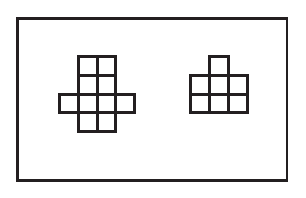
\includegraphics[width=0.73\linewidth]{images/SumPrinc}
\caption{The union of these two disjoint sets has size 17.\label{sumprinc}}
\end{figure}
\begin{figure}
\centering
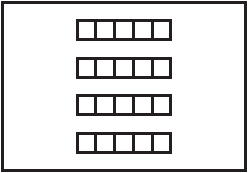
\includegraphics[width=0.73\linewidth]{images/ProdPrinc}
\caption{The union of four disjoint sets of size five.\label{prodprinc}}
\end{figure}
You may have noticed some standard mathematical words and phrases such as \emph{set}, \emph{ordered pair}, \emph{function} and so on creeping into the problems. One of our goals in these notes is to show how most counting problems can be recognized as counting all or some of the elements of a set of standard mathematical objects. For example \hyperref[orderedpair]{Problem~\ref{orderedpair}} is meant to suggest that the question we asked in \hyperref[basicsandwiches]{Problem~\ref{basicsandwiches}} was really a problem of counting all the ordered pairs consisting of a bread choice and a filling choice. We use \(A\times B\) to stand for the set of all ordered pairs whose first element is in \(A\) and whose second element is in \(B\) and we call \(A\times B\) the \index{Cartesian product}\index{product!Cartesian}\terminology{Cartesian product} of \(A\) and \(B\), so you can think of \hyperref[orderedpair]{Problem~\ref{orderedpair}} as asking you for the size of the Cartesian product of \(M\) and \(N\), that is, asking you to count the number of elements of this Cartesian product.%
\par
When a set \(S\) is a union of disjoint sets \(B_1, B_2, \ldots, B_m\) we say that the sets \(B_1, B_2, \ldots, B_m\) are a \terminology{partition}\index{partition!of a set} of the set \(S\). Thus a partition of \(S\) is a (special kind of) set of sets. So that we don't find ourselves getting confused between the set \(S\) and the sets \(B_i\) into which we have divided it, we often call the sets \(B_1, B_2,
\ldots, B_m\) the \emph{blocks}\index{partition!blocks of}\index{block of a partition} of the partition. In this language, the \index{principle!sum}\index{sum principle}\terminology{sum principle}says that%
\begin{quote}if we have a partition of a set \(S\), then the size of \(S\) is the sum of the sizes of the blocks of the partition.%
\end{quote}
The \index{principle!product}\index{product principle}\terminology{product principle} says that%
\begin{quote}if we have a partition of a set \(S\) into \(m\) blocks, each of size \(n\), then \(S\) has size \(mn\).%
\end{quote}
You'll notice that in our formal statement of the sum and product pinciple we talked about a partition of a finite set. We could modify our language a bit to cover infinite sizes, but whenever we talk about sizes of sets in what follows, we will be working with finite sets. So as to avoid possible complications in the future, let us agree that when we refer to the size of a set, we are implicitly assuming the set is finite. There is another version of the product principle that applies directly in problems like \hyperref[completelunch]{Problem~\ref{completelunch}} and \hyperref[tripledeckercone]{Problem~\ref{tripledeckercone}}, where we were not just taking a union of \(m\) disjoint sets of size \(n\), but rather \(m\) disjoint sets of size \(n\), each of which was a union of \(m'\) disjoint sets of size \(n'\). This is an inconvenient way to have to think about a counting problem, so we may rephrase the product principle in terms of a sequence of decisions:%
\begin{activity}[]\label{generalproductprincipleintro}
If we make a sequence of \(m\) choices for which \leavevmode%
\begin{itemize}[label=\textbullet]
\item{}there are \(k_1\) possible first choices, and%
\item{}for each way of making the first \(i-1\) choices, there are \(k_i\) ways to make the \(i\)th choice,%
\end{itemize}
 then in how many ways may we make our sequence of choices? (You need not prove your answer correct at this time.)%
\end{activity}
The counting principle you gave in \hyperref[generalproductprincipleintro]{Problem~\ref{generalproductprincipleintro}} is called the \emph{general product principle}.\index{general product principle}\index{product principle!general}\index{principle!product!general} We will outline a proof of the general product pinciple from the original product principle in \hyperref[generalproductprincipleproof]{Problem~\ref{generalproductprincipleproof}}. Until then, let us simply accept it as another counting principle. For now, notice how much easier it makes it to explain why we multiplied the things we did in \hyperref[completelunch]{Problem~\ref{completelunch}} and \hyperref[tripledeckercone]{Problem~\ref{tripledeckercone}}.%
\begin{activity}[]\label{tennispairings1}
A tennis club has \(2n\) members. We want to pair up the members by twos for singles matches.%
~\par
\begin{enumerate}[label=(\alph*)]
 \item In how many ways may we pair up all the members of the club? (Hint: consider the cases of 2, 4, and 6 members.)%
\par\medskip\noindent%
\textbf{Hint.}\quad Suppose you have a list in alphabetical order of names of the members of the club. In how many ways can you pair up the first person on the list? In how many ways can you pair up the next person who isn’t already paired up?%
\par\medskip\noindent%
\textbf{Solution.}\quad Suppose we list the people in the club in some way, and keep that list for the remainder of the problem. Take the first person from the list and pair that person with any of the \(2n-1\) remaining people. Now take the next \emph{unpaired} person from the list and pair that person with any of the remaining \(2n-3\) unpaired people. Continuing in this way, once \(k\) pairs have been selected, take the next unpaired person from the list and pair that person with any of the remaining \(2n-2k-1\) unpaired people. Every pairing can arise in this way, and no pairing can arise twice in this process. Thus the number of outcomes is \(\prod_{i=0}^{n-1} 2n-2i-1\).%

~\par
\item Suppose that in addition to specifying who plays whom, for each pairing we say who serves first.  Now in how many ways may we specify our pairs?%

\end{enumerate}
\end{activity}
\begin{activity}[]\label{countingfunctions2}
Let us now return to \hyperref[countingfunctions]{Problem~\ref{countingfunctions}} and justify\textemdash{}or perhaps finish\textemdash{}our answer to the question about the number of functions from a three-element set to a 12-element set.%
~\par
\begin{enumerate}[label=(\alph*)]
 \item How can you justify your answer in \hyperref[countingfunctions]{Problem~\ref{countingfunctions}} to the question ``How many functions are there from a three element set (say \([3]=\{1,2,3\}\)) to a twelve element set (say [12])?''%
\par\medskip\noindent%
\textbf{Solution.}\quad The number of functions from \([3]\) to \([12]\) with \(f(3) =1\) is the number of functions from \([2]\) to \([12]\), namely 144. The same is true for the number of functions with \(f(3)=2\) and \(f(3)=3\), and the size of the set \(S_i\). The union of the sets \(S_i\) is the set of all functions from \([3]\) to \([12]\), and since there are twelve sets \(S_i\), this union has size \(12\cdot144= 1728\).%

~\par
\item Based on the examples you've seen so far, make a conjecture about how many functions there are from the set%
\begin{equation*}
[m] = \{1,2,3,\dots,m\}
\end{equation*}
to \([n]=\{1,2,3,\dots,n\}\) and prove it.%
\par\medskip\noindent%
\textbf{Solution.}\quad \(n^m\).%

~\par
\item A common notation for the set of all functions from a set \(M\) to a set \(N\) is \(N^M\).  Why is this a good notation?%
\par\medskip\noindent%
\textbf{Solution.}\quad Because there are \(n^m\) such functions, at least according to our conjecture.%

\end{enumerate}
\end{activity}
\begin{activity}[]\label{generalproductprinciple}
Now suppose we are thinking about a set \(S\) of functions \(f\) from \([m]\) to some set \(X\). (For example, in \hyperref[tripledeckercone]{Problem~\ref{tripledeckercone}} we were thinking of the set of functions from the three possible places for scoops in an ice-cream cone to \(12\) flavors of ice cream.) Suppose there are \(k_1\) choices for \(f(1)\). (In \hyperref[tripledeckercone]{Problem~\ref{tripledeckercone}}, \(k_1\) was \(12\), because there were \(12\) ways to choose the first scoop.) Suppose that for each choice of \(f(1)\) there are \(k_2\) choices for \(f(2)\). (For example, in \hyperref[tripledeckercone]{Problem~\ref{tripledeckercone}} \(k_2\) was \(12\) if the second flavor could be the same as the first, but \(k_2\) was \(11\) if the flavors had to be different.) In general, suppose that for each choice of \(f(1)\), \(f(2)\), \dots{} \(f(i-1)\), there are \(k_i\) choices for \(f(i)\). (For example, in \hyperref[tripledeckercone]{Problem~\ref{tripledeckercone}}, if the flavors have to be different, then for each coice of \(f(1)\) and \(f(2)\), there are \(10\) choices for \(f(3)\).)%
\par
What we have assumed so far about the functions in \(S\) may be summarized as \leavevmode%
\begin{itemize}[label=\textbullet]
\item{}There are \(k_1\) choices for \(f(1)\).%
\item{}For each choice of \(f(1)\), \(f(2)\), \dots{}, \(f(i-1)\), there are \(k_i\) choices for~\(f(i)\).%
\end{itemize}
%
\par
How many functions are in the set \(S\)? Is there any practical difference between the result of this problem and the general product principle?%
\par\medskip\noindent%
\textbf{Solution.}\quad \(\prod_{i=1}^m k_i\).%
\end{activity}
The point of \hyperref[generalproductprinciple]{Problem~\ref{generalproductprinciple}} is that the general product principle can be stated informally, as we did originally, or as a statement about counting sets of standard concrete mathematical objects, namely functions.%
\begin{activity}[]\label{activity-15}
A roller coaster car has \(n\) rows of seats, each of which has room for two people. If \(n\) men and \(n\) women get into the car with a man and a woman in each row, in how many ways may they choose their seats?%
\par\medskip\noindent%
\textbf{Hint.}\quad In how many ways may you assign the men to their rows? The women? Once a woman and a man have a row to share, in how many ways may they choose their seats?%
\par\medskip\noindent%
\textbf{Solution.}\quad \((n!)^22^n\)%
\end{activity}
\begin{activity}[]\label{activity-16}
How does the general product principle apply to \hyperref[tripledeckercone]{Problem~\ref{tripledeckercone}}?%
\par\medskip\noindent%
\textbf{Solution.}\quad By the general product principle, there are \(12\cdot 11\cdot 10\) triple decker cones.%
\end{activity}
\begin{activity}[]\label{activity-17}
In how many ways can we pass out \(k\) distinct pieces of fruit to \(n\) children (with no restriction on how many pieces of fruit a child may get)?%
\par\medskip\noindent%
\textbf{Solution.}\quad Either by the formula for the number of functions from an \(m\)-element set to an \(n\)-element set or the general product principle, there are \(k^n\) ways. (Each distribution is a function from the set of fruit to the set of children, because each piece of fruit goes to one and only one child.)%
\end{activity}
\begin{activity}[]\label{SubsetsFirstTime}
How many subsets does a set \(S\) with \(n\) elements have?%
\par\medskip\noindent%
\textbf{Hint.}\quad Try applying the product principle in the case n = 2 and n = 3. How might you apply it in general?%
\par\medskip\noindent%
\textbf{Solution.}\quad For each of the \(n\) elements of \(S\), we have two options: either we put the element into the subset or we do not. Thus, the general product principle tells us that there are \(2^n\) subsets of \(S\).%
\end{activity}
\begin{activity}[]\label{activity-19}
Assuming \(k\le n\), in how many ways can we pass out \(k\) distinct pieces of fruit to \(n\) children if each child may get at most one? What is the number if \(k>n\)? Assume for both questions that we pass out all the fruit.%
\par\medskip\noindent%
\textbf{Hint.}\quad Ask yourself if either the sum principle or product principle applies.%
\par\medskip\noindent%
\textbf{Hint.}\quad Remember that zero is a number.%
\par\medskip\noindent%
\textbf{Solution.}\quad We are asking for the number of \(k\)-element permutations of \(n\) children, which is \(\prod_{i=1}^k n-i+1\), and is zero if \(k>n\).%
\end{activity}
\begin{activity}[]\label{kelementpermutation}
Another name for a list, in a specific order, of \(k\) distinct things chosen from a set \(S\) is a \terminology{\(k\)-element permutation} of \(S\).\index{permutation!\(k\)-element} We can also think of a \(k\)-element permutation of \(S\) as a one-to-one function (or, in other words, injection) from \([k]=\{1,2,\ldots, k\}\) to \(S\). How many \(k\)-element permutations does an \(n\)-element set have? (For this problem it is natural to assume \(k\le n\). However the question makes sense even if \(k>n\). What is the number of \(k\)-element permutations of an \(n\)-element set if \(k>n\)?%
\par\medskip\noindent%
\textbf{Hint.}\quad Do you see an analogy between this problem and any of the previous problems?%
\par\medskip\noindent%
\textbf{Solution.}\quad By the general product principle, the number is%
\begin{equation*}
\prod_{i=1}^k(n-i+1).
\end{equation*}
In the case that \(k>n\), there are no such lists with distinct entries, and that is what the formula gives us, because \(n-(n+1)+1=0\).%
\end{activity}
There are a number of different notations for the number of \(k\)-element permutations of an \(n\)-element set. The one we shall use was introduced by Don Knuth; namely \(n^{\underline{k}}\), read ``\(n\) to the \(k\) falling'' or ``\(n\) to the \(k\) down''. In \hyperref[kelementpermutation]{Problem~\ref{kelementpermutation}} you may have shown that%
\begin{equation}
n^{\underline{k}} =n(n-1)\cdots (n-k+1)= \prod_{i=1}^k(
n-i+1).\label{productnotation}
\end{equation}
%
\par
It is standard to call \(n^{\underline{k}}\)\index{\(n^{\underline{k}}\)} the \terminology{\(k\)-th falling factorial power of \(n\)}\index{falling factorial power}\index{factorial power!falling}, which explains why we use exponential notation. Of course we call it a \emph{factorial} power since \(n^{\underline{n}} = n(n-1)\cdots 1\) which we call \emph{\(n\)-factorial} and denote by \(n!\).\index{factorial}\index{\(n"!\)} If you are unfamiliar with the \(\Pi\) notation, or \terminology{product notation}\index{product notation}\index{\(Pi\) notation} we introduced for products in \hyperref[productnotation]{Equation~(\ref{productnotation})}, it works just like the \(\Sigma\) notation works for summations.%
\begin{activity}[]\label{activity-21}
Express \(n^{\underline{k}}\) as a quotient of factorials.%
\par\medskip\noindent%
\textbf{Solution.}\quad \(n^{\underline{k}}=n!/(n-k)!\)%
\end{activity}
\begin{activity}[]\label{activity-22}
How should we define \(n^{\underline{0}}\)?%
\par\medskip\noindent%
\textbf{Solution.}\quad We define \(n^{\underline{0}}\) to be \(1\).%
\end{activity}
\typeout{************************************************}
\typeout{Subsection  Functions and directed graphs}
\typeout{************************************************}
\subsection[{Functions and directed graphs}]{Functions and directed graphs}\label{subsection-2}
As another example how standard mathematical language relates to counting problems, \hyperref[countingfunctions]{Problem~\ref{countingfunctions}} explicitly asked you to relate the idea of counting functions to the question of \hyperref[tripledeckercone]{Problem~\ref{tripledeckercone}}. You have probably learned in algebra or calculus how to draw graphs in the Cartesian plane of functions from a set of numbers to a set of numbers. You may recall how we can determine whether a graph is a graph of a function by examining whether each vertical straight line crosses the graph at most one time. You might also recall how we can determine whether such a function is one-to-one by examining whether each horizontal straight line crosses the graph at most one time. The functions we deal with will often involve objects which are not numbers, and will often be functions from one finite set to another. Thus graphs in the cartesian plane will often not be available to us for visualizing functions.%
\par
However, there is another kind of graph called a \emph{directed graph}\index{graph!directed}\index{directed graph} or \emph{digraph}\index{digraph}\index{function!digraph of} that is especially useful when dealing with functions between finite sets. We take up this topic in more detail in \hyperref[Relations]{Appendix~\ref{Relations}}, particularly \hyperref[relationdigraph]{Section~} and \hyperref[digraphsoffunctions]{Section~}. In \hyperref[functiondigraphs]{Figure~\ref{functiondigraphs}} we show several examples of digraphs of functions.%
\begin{figure}
\centering
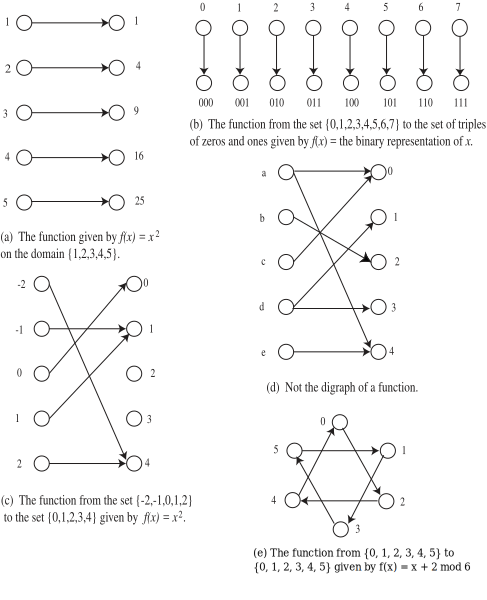
\includegraphics[width=0.73\linewidth]{images/functiondigraph}
\caption{What is a digraph of a function?\label{functiondigraphs}}
\end{figure}
If we have a function \(f\) from a set \(S\) to a set \(T\), we draw a line of dots or circles, called \emph{vertices} to represent the elements of \(S\) and another (usually parallel) line of circles or dots to represent the elements of \(T\). We then draw an arrow from the circle for \(x\) to the circle for \(y\) if \(f(x) = y\). Sometimes, as in part (e) of the figure, if we have a function from a set \(S\) to itself, we draw only one set of vertices representing the elements of \(S\), in which case we can have arrows both entering and leaving a given vertex. As you see, the digraph can be more enlightening in this case if we experiment with the function to find a nice placement of the vertices rather than putting them in a row.%
\par
\emph{The figure needs to have part (e) added to it.}%
\par
Notice that there is a simple test for whether a digraph whose vertices represent the elements of the sets \(S\) and \(T\) is the digraph of a function from \(S\) to \(T\). There must be one and only one arrow leaving each vertex of the digraph representing an element of \(S\). The fact that there is one arrow means that \(f(x)\) is defined for each \(x\) in \(S\). The fact that there is only one arrow means that each \(x\) in \(S\) is related to exactly one element of \(T\). (Note that these remarks hold as well if we have a function from \(S\) to \(S\) and draw only one set of vertices representing the elements of \(S\).) For further discussion of functions and digraphs see \hyperref[functionrelation]{Sections~} and \hyperref[relationdigraph]{Subsection~} of {\hyperref[Relations]{Appendix~\ref{Relations}}}.%
\begin{activity}[]\label{activity-23}
Draw the digraph of the function from the set \(\{\)Alice, Bob, Dawn, Bill\(\}\) to the set \(\{\)A, B, C, D, E\(\}\) given by%
\begin{equation*}
f(X) = \mbox{the first
letter of the name \(X\)} .
\end{equation*}
%
\end{activity}
\begin{activity}[]\label{activity-24}
A function \(f:S\rightarrow T\) is called an \index{onto function}\index{function!onto}\emph{onto function} or \index{surjection}\index{function!surjection}\emph{surjection} if each element of \(T\) is \(f(x)\) for some \(x\in S\). Choose a set \(S\) and a set \(T\) so that you can draw the digraph of a function from \(S\) to \(T\) that is one-to-one but not onto, and draw the digraph of such a function.%
\par\medskip\noindent%
\textbf{Solution.}\quad The digraph of one such function follows%
\par
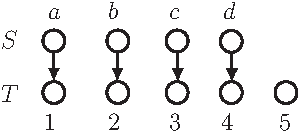
\includegraphics[width=0.73\linewidth]{images/OnetoOneNotOnto}
%
\end{activity}
\begin{activity}[]\label{activity-25}
Choose a set \(S\) and a set \(T\) so that you can draw the digraph of a function from \(S\) to \(T\) that is onto but not one-to-one, and draw the digraph of such a function.%
\par\medskip\noindent%
\textbf{Solution.}\quad The digraph of one such function follows%
\par
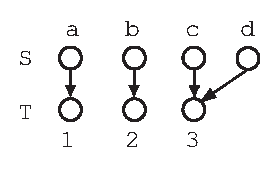
\includegraphics[width=0.73\linewidth]{images/OntoNotOnetoOne}
%
\end{activity}
\begin{activity}[]\label{activity-26}
Digraphs of functions help us visualize the ideas of one-to-one functions and onto functions.%
~\par
\begin{enumerate}[label=(\alph*)]
 \item What does the digraph of a one-to-one function (injection) from a finite set \(X\) to a finite set \(Y\) look like? (Look for a test somewhat similar to the one we described for when a digraph is the digraph of a function.)%

~\par
\item What does the digraph of an onto function look like?%

~\par
\item What does the digraph of a one-to-one and onto function from a finite set \(S\) to a set \(T\) look like?%

\end{enumerate}
\par\medskip\noindent%
\textbf{Hint.}\quad For each part of this problem, think about how many arrows are allowed to enter a vertex representing a member of \(Y\).%
\par\medskip\noindent%
\textbf{Solution.}\quad One-to-one: One arrow comes out of each vertex representing a member of \(X\) and at most one arrow goes into each vertex representing a member of \(Y\). Onto: : One arrow comes out of each vertex representing a member of \(X\) and at least one arrow goes into each vertex representing a member of \(Y\). One-to-one and onto: One arrow comes out of each vertex representing a member of \(X\) and at exactly one arrow goes into each vertex representing a member of \(Y\). (The first half of each sentence is optional.)%
\end{activity}
\begin{activity}[]\label{permutationasbijection}
The word \emph{permutation} is actually used in two different ways in mathematics. A \terminology{permutation}\index{permutation!as a bijection} of a set \(S\) is one-to-one from \(S\) onto \(S\). How many permutations does an \(n\)-element set have?%
\par\medskip\noindent%
\textbf{Solution.}\quad \(n!\).%
\end{activity}
Notice that there is a great deal of consistency between the use of the word permutation in \hyperref[permutationasbijection]{Problem~\ref{permutationasbijection}} and the use in \hyperref[kelementpermutation]{Problem~\ref{kelementpermutation}}. If we have some way \(a_1,a_2,\ldots,a_n\) of listing our set, then any other list \(b_1,b_2,\ldots,b_n\) gives us the permutation of \(S\) whose rule is \(f(a_i) =b_i\), and any permutation of \(S\), say the one given by \(g(a_i)=c_i\) gives us a list \(c_1,c_2,\ldots,c_n\) of \(S\). Thus there is really very little difference between the idea of a permutation of \(S\) and an \(n\)-element permutation of \(S\) when \(n\) is the size of \(S\).%
\typeout{************************************************}
\typeout{Subsection  The bijection principle}
\typeout{************************************************}
\subsection[{The bijection principle}]{The bijection principle}\label{subsection-3}
Another name for a one-to-one and onto function is \index{bijection}\index{function!bijection}\terminology{bijection}. The digraphs marked (a), (b), and (e) in \hyperref[functiondigraphs]{Figure~\ref{functiondigraphs}} are digraphs of bijections. The description in \hyperref[bijectiondigraph]{Problem~} of the digraph of a bijection from \(X\) to \(Y\) illustrates one of the fundamental principles of combinatorial mathematics, the \index{principle!bijection}\index{bijection principle}\terminology{bijection principle}:%
\begin{quote}Two sets have the same size if and only if there is a bijection between them.%
\end{quote}
It is surprising how this innocent sounding principle guides us into finding insight into some otherwise very complicated proofs.%
\typeout{************************************************}
\typeout{Subsection  Counting subsets of a set}
\typeout{************************************************}
\subsection[{Counting subsets of a set}]{Counting subsets of a set}\label{subsection-4}
\begin{activity}[]\label{SubsetsBinaryRepresentation}
The \terminology{binary representation} of a number \(m\) is a list, or string, \(a_1a_2\ldots a_k\) of zeros and ones such that \(m=a_12^{k-1} + a_2 2^{k-2}
+\cdots+ a_k 2^0.\) Describe a bijection between the binary representations of the integers between 0 and \(2^n-1\) and the subsets of an \(n\)-element set. What does this tell you about the number of subsets of an \(n\)-element set?%
\par\medskip\noindent%
\textbf{Hint.}\quad The problem is asking you to describe a one-to-one function from the set of binary representations of numbers between \(0\) and \(2^n-1\) onto the set of subsets of the set \([n]\). Write down these two sets for \(n = 2\). They should both have four elements. The set of binary representations should contain the string \(00\). You could think of this as the instruction ``take no ones and take no twos.'' In that context, what could you think of the string \(11\) as standing for? This should help you describe a function. Of course now you have to figure out how to show it is one-to-one and onto.%
\par\medskip\noindent%
\textbf{Solution.}\quad The sequence \(a_1a_2\ldots
a_k\) corresponds to the set of \(i\) such that \(a_i = 1\). This is a bijection because each sequence gives a set, and each set can be the set of places where a sequence is 1. Since there are \(2^n\) integers which are between 0 and \(2^n-1\), and they correspond to sequences of length \(n\) (notice, we have another bijection, the one between a number and its binary representation), there are \(2^n\) subsets of the \(n\)-element set \([n]\).%
\end{activity}
Notice that the first question in \hyperref[icecreaminpints]{Problem~\ref{icecreaminpints}} asked you for the number of ways to choose a three element subset from a 12 element subset. You may have seen a notation like \(\binom{n}{k}\), \(C(n,k)\), or \(_nC_k\) which stands for the number of ways to choose a \(k\)-element subset from an \(n\)-element set. The number \(\binom{n}{k}\) is read as ``\(n\) choose \(k\)'' and is called a \index{binomial coefficient}\terminology{binomial coefficient} for reasons we will see later on. Another frequently used way to read the binomial coefficient notation is ``the number of combinations \index{combinations} of \(n\) things taken \(k\) at a time." You are going to be asked to construct two bijections that relate to these numbers and figure out what famous formula they prove. We are going to think about subsets of the \(n\)-element set \([n] =
\{1,2,3,\ldots, n\}\). As an example, the set of two-element subsets of \([4]\) is%
\begin{equation*}
\{\{1,2\}, \{1,3\}, \{1,4\}, \{2,3\}, \{2,4\}, \{3,4\}\}.
\end{equation*}
%
\par
This example tells us that \(\binom{4}{2} = 6\).%
\begin{activity}[]\label{Pascal}
Let \(C\) be the set of \(k\)-element subsets of \([n]\) that contain the number \(n\), and let \(D\) be the set of \(k\)-element subsets of \([n]\) that don't contain \(n\).%
~\par
\begin{enumerate}[label=(\alph*)]
 \item Let \(C'\) be the set of \((k-1)\)-element subsets of \([n-1]\).  Describe a bijection from \(C\) to \(C'\).  (A verbal description is fine.)%
\par\medskip\noindent%
\textbf{Solution.}\quad Let \(f(X) = X-\{n\}\), the set \(X\) with \(n\) removed. This is a bijection because two different sets containing \(n\) must yield different sets when \(n\) is removed (one-to-one), and each \((k-1)\)-element subset \(X\) of \([n-1]\) may be obtained from the \(k\)-element subset \(X\cup \{n\}\) of \([n]\) by removing \(n\) (onto).%

~\par
\item Let \(D'\) be the set of \(k\)-element subsets of \([n-1]=\{1,2,\ldots n-1\}\).  Describe a bijection from \(D\) to \(D'\). (A verbal description is fine.)%
\par\medskip\noindent%
\textbf{Solution.}\quad Simply let \(f(X) =X\). This is one-to-one by definition, and onto because the subsets of \([n-1]\) are identical with the subsets of \([n]\) not containing \(n\).%

~\par
\item Based on the two previous parts, express the sizes of \(C\) and \(D\) in terms of binomial coefficients involving \(n-1\) instead of \(n\).%
\par\medskip\noindent%
\textbf{Solution.}\quad \(|C|= \binom{n-1}{k-1}\); \(|D| = \binom{n-1}{k}\)%

~\par
\item Apply the sum principle to \(C\) and \(D\) and obtain a formula that expresses \(\binom{n}{k}\) in terms of two binomial coefficients involving \(n-1\).  You have just derived the Pascal Equation that is the basis for the famous Pascal's Triangle.%
\par\medskip\noindent%
\textbf{Solution.}\quad \(\binom{n}{k} = \binom{n-1}{k-1} +\binom{n-1}{k}\).%

\end{enumerate}
\end{activity}
\typeout{************************************************}
\typeout{Subsection  Pascal's Triangle}
\typeout{************************************************}
\subsection[{Pascal's Triangle}]{Pascal's Triangle}\label{subsection-5}
The Pascal Equation that you derived in \hyperref[Pascal]{Problem~\ref{Pascal}} gives us the triangle in \hyperref[Pascaltriangle]{Figure~\ref{Pascaltriangle}}. This figure has the number of \(k\)-element subsets of an \(n\)-element set as the \(k\)th number over in the \(n\)th row (we call the top row the zeroth row and the beginning entry of a row the zeroth number over). You'll see that your formula doesn't say anything about \(\binom{n}{k}\) if \(k=0\) or \(k=n\), but otherwise it says that each entry is the sum of the two that are above it and just to the left or right.%
\begin{figure}
\centering
\index{Pascal's Triangle}%
\begin{equation*}
\begin{matrix}\amp \amp \amp \amp \amp \amp \amp 1\amp \amp \amp \amp \amp \amp \amp \\
\amp \amp \amp \amp \amp \amp 1\amp \amp 1\amp \amp \amp \amp \amp \amp \\
\amp \amp \amp \amp \amp 1\amp \amp 2\amp \amp 1\amp \amp \amp \amp \amp \\
\amp \amp \amp \amp 1\amp \amp 3\amp \amp 3\amp \amp 1\amp \amp \amp \amp \\
\amp \amp \amp 1\amp \amp 4\amp \amp 6\amp \amp 4\amp \amp 1\amp \amp \\
\amp \amp 1\amp \amp 5\amp \amp 10\amp \amp 10\amp \amp 5\amp \amp 1\amp \\
\amp 1\amp \amp 6\amp \amp 15\amp \amp 20\amp \amp 15\amp \amp 6\amp \amp 1\\
1\amp \amp 7\amp \amp 21\amp \amp 35\amp \amp 35\amp \amp 21\amp \amp 7\amp \amp 1
\end{matrix}
\end{equation*}
%
\caption{Pascal's Triangle\label{Pascaltriangle}}
\end{figure}
\begin{activity}[]\label{activity-30}
Just for practice, what is the next row of Pascal's triangle?%
\par\medskip\noindent%
\textbf{Solution.}\quad %
\begin{equation*}
1 \quad 8 \quad 28 \quad 56 \quad 70 \quad 56 \quad 28 \quad 8 \quad 1
\end{equation*}
%
\end{activity}
\begin{activity}[]\label{activity-31}
Without writing out the rows completely, write out enough of Pascal's triangle to get a numerical answer for the first question in \hyperref[icecreaminpints]{Problem~\ref{icecreaminpints}}.%
\par\medskip\noindent%
\textbf{Hint.}\quad Starting with the row 1 8 28 56 70 56 28 8 1, put dots below it where the elements of row 9 should be. Then put dots below that where the elements of row 10 should be. Do the same for rows 11 and 12. Mark the dot where row 12 should appear. Now mark the dots you need in row 11 to compute the entry in column 3 of row 12. Now mark the dots you need in row 10 to compute the marked entries in row 11. Do the same for rows 9 and 8. Now you should be able to see what you need to do.%
\par\medskip\noindent%
\textbf{Solution.}\quad Starting with row 9, we get%
\begin{equation*}
\begin{matrix}\amp \amp \amp 1\amp \amp 9\amp \amp 36\amp \amp 84 \cr\amp \amp 1\amp \amp 10\amp \amp 45\amp \amp 120\cr\amp 1\amp \amp 11\amp \amp 55\amp \amp 165\cr
1\amp \amp 12\amp \amp 66\amp \amp 220
\end{matrix}
\end{equation*}
so the answer is 220.%
\end{activity}
It is less common to see Pascal's triangle as a right triangle, but it actually makes your formula easier to interpret. In Pascal's Right Triangle, the element in row \(n\) and column \(k\) (with the convention that the first row is row zero and the first column is column zero) is \(\binom{n}{k}\). In this case your formula says each entry in a row is the sum of the one above and the one above and to the left, except for the leftmost and rightmost entries of a row, for which that doesn't make sense. Since the leftmost entry is \(\binom{n}{0}\) and the rightmost entry is \(\binom{n}{n}\), these entries are both one (to see why, ask yourself how many \(0\)-element subsets and how many \(n\)-element subsets an \(n\)-element set has), and your formula then tells how to fill in the rest of the table.%
\begin{table}
\centering
\begin{tabular}{lllllllll}
&\(k=0\)&1&2&3&4&5&6&7\tabularnewline[0pt]
&&&&&&&&\tabularnewline\hrulethin
\(n=0\)&1&&&&&&\tabularnewline[0pt]
1&1&1&&&&&\tabularnewline[0pt]
2&1&2&1&&&&&\tabularnewline[0pt]
3&1&3&3&1&&&&\tabularnewline[0pt]
4&1&4&6&4&1&&&\tabularnewline[0pt]
5&1&5&10&10&5&1&&\tabularnewline[0pt]
6&1&6&15&20&15&6&1&\tabularnewline[0pt]
7&1&7&21&35&35&21&7&1
\end{tabular}
\caption{Pascal's Right Triangle\label{Pascalrighttriangle}}
\end{table}
Seeing this right triangle leads us to ask whether there is some natural way to extend the right triangle to a rectangle. If we did have a rectangular table of binomial coefficients, counting the first row as row zero (i.e., \(n=0\)) and the first column as column zero (i.e., \(k=0\)), the entries we don't yet have are values of \(\binom{n}{k}\) for \(k>n\). But how many \(k\)-element subsets does an \(n\)-element set have if \(k>n\)? The answer, of course, is zero, so all the other entries we would fill in would be zero, giving us the rectangular array in \hyperref[Pascal_sRectangle]{Figure~\ref{Pascal_sRectangle}}. It is straightforward to check that Pascal's equation now works for all the entries in the rectangle that have an entry above them and an entry above and to the left.%
\begin{table}
\centering
\begin{tabular}{lllllllll}
&\(k=0\)&1&2&3&4&5&6&7\tabularnewline[0pt]
&&&&&&&&\tabularnewline\hrulethin
\(n=0\)&1&0&0&0&0&0&0&0\tabularnewline[0pt]
1&1&1&0&0&0&0&0&0\tabularnewline[0pt]
2&1&2&1&0&0&0&0&0\tabularnewline[0pt]
3&1&3&3&1&0&0&0&0\tabularnewline[0pt]
4&1&4&6&4&1&0&0&0\tabularnewline[0pt]
5&1&5&10&10&5&1&0&0\tabularnewline[0pt]
6&1&6&15&20&15&6&1&0\tabularnewline[0pt]
7&1&7&21&35&35&21&7&1
\end{tabular}
\caption{Pascal's Rectangle\label{Pascal_sRectangle}}
\end{table}
\begin{activity}[]\label{activity-32}
Because our definition told us that \(\binom{n}{k}\) is 0 when \(k>n\), we got a rectangular table of numbers that satisfies the Pascal Equation.%
~\par
\begin{enumerate}[label=(\alph*)]
 \item Is there any other way to define \(\binom{n}{k}\) when \(k>n\) in order to get a rectangular table that agrees with Pascal's Right Triangle for \(k\le n\) and satisfies the Pascal Equation?%
\par\medskip\noindent%
\textbf{Hint.}\quad Begin by trying to figure out what the entries just above the diagonal of the rectangle are. After that, what other entries can you figure out?%
\par\medskip\noindent%
\textbf{Solution.}\quad No, because there must be a zero above each one not in column zero. Then above each zero not in column zero or one, there must be yet another zero and so on.%

~\par
\item Suppose we want to extend Pascal's Rectangle to the left and define \(\binom{n}{-k}\) for \(n\ge 0\) and \(k>0\) so that \(-k\lt 0\). What should we put into row \(n\) and column \(-k\) of Pascal's Rectangle in order for the Pascal Equation to hold true?%
\par\medskip\noindent%
\textbf{Hint.}\quad See if you can figure out what the entries in column \(-1\) have to be.%
\par\medskip\noindent%
\textbf{Solution.}\quad To the left of all the ones in column zero, we must have zeros for the Pascal Equation to hold. To the left of those zeros, we must again have zeros, and so on.%

~\par
\item What should we put into row \(-n\) and column \(k\) or column \(-k\) in order for the Pascal Equation to continue to hold?  Do we have any freedom of choice?%
\par\medskip\noindent%
\textbf{Hint.}\quad What does the sum of two consecutive values in row \(-1\) have to be? Could this sum depend on which two consecutive values we take? Is there some value of row \(-1\) that we could choose arbitrarily? Now what about row \(-2\)?  Can we make arbitrary choices there? If so, how many can we make, and is their position arbitrary?%
\par\medskip\noindent%
\textbf{Solution.}\quad Above row zero, we have some freedom. The \(-1,-1\) and the \(-1,0 \)entry must add to one, so they can be \(-x\) and \(x+1\) for any number \(x\). To the right of the \(-1,0\) entry they must alternate between \((-x-1)\) and \(x+1\) while to the left of the \(-1,1\) entry they must alternate between \(-x\) and \(x\), ending with the \(-x\) in position \(-1,1\). Now if we know the entry in row \(-2\) and column 0, we can use the Pascal equation (in the form \(\binom{n-1}{k-1} = \binom{n}{k} - \binom{n-1}{k}\)) to compute all the entries to the left of it, and (in a different form) to compute all the entries to the right of it. Thus we may be arbitrary about the entries in column 0 (or, in fact, one entry in each row) and then the Pascal Equation tells us how to fill in the rest of each row. We shall see later on that there is one very natural choice for how to fill in all the rows above row zero.%

\end{enumerate}
\end{activity}
\begin{activity}[]\label{charfunction}
There is yet another bijection that lets us prove that a set of size \(n\) has \(2^n\) subsets. Namely, for each subset \(S\) of \([n]=\{1,2,\ldots, n\}\), define a function (traditionally denoted by \(\chi_S\)) as follows.\footnote{The symbol \(\chi\) is the Greek letter chi that is pronounced Ki, with the \(i\) sounding like ``eye.''\label{fn-1}}%
\begin{equation*}
\chi_S(i) = \begin{cases}1 \amp \mbox{ if }  i\in S \\ 0 \amp \mbox{ if }  i\not\in
S
\end{cases}
\end{equation*}
%
\par
The function \(\chi_S\) is called the \index{characteristic function}\index{function!characteristic}\terminology{characteristic function} of \(S\). Notice that the characteristic function is a function from \([n]\) to \(\{0,1\}\).%
~\par
\begin{enumerate}[label=(\alph*)]
 \item For practice, consider the function \(\chi_{\{1,3\}}\) for the subset \(\{1,3\}\) of the set \(\{1,2,3,4\}\).  What are \leavevmode%
\begin{enumerate}[label=(\roman*)]
\item\hypertarget{li-5}{}\(\chi_{\{1,3\}}(1)\)?%
\item\hypertarget{li-6}{}\(\chi_{\{1,3\}}(2)\)?%
\item\hypertarget{li-7}{}\(\chi_{\{1,3\}}(3)\)?%
\item\hypertarget{li-8}{}\(\chi_{\{1,3\}}(4)\)?%
\end{enumerate}
%

~\par
\item We define a function \(f\) from the set of subsets of \([n]=\{1,2,\ldots, n\}\) to the set of functions from \([n]\) to \(\{0,1\}\) by \(f(S)=\chi_S\).  Explain why \(f\) is a bijection.%
\par\medskip\noindent%
\textbf{Solution.}\quad If \(i\in S\) but \(i\not\in T\), then \(\chi_S(i)=1\) but \(\chi_T(i)=0\). Thus if \(S\not= T\), the \(\chi_S\not=\chi_T\). Therefore \(f\) is one-to-one. Given a function \(g\) from \([n]\) to \(\{0,1\}\), let \(S=\{i|g(i)=1\}\). Then by definition, \(g=\chi_S=f(S)\). Therefore \(f\) is onto, so it is a bijection.%

~\par
\item Why does the fact that \(f\) is a bijection prove that \([n]\) has \(2^n\) subsets?%
\par\medskip\noindent%
\textbf{Solution.}\quad We have seen that there are \(2^n\) functions from \([n]\) to a two-element set, and we have a bijection between the set of all such functions and the subsets of \([n]\).%

\end{enumerate}
\end{activity}
In \hyperref[SubsetsFirstTime]{Problems~\ref{SubsetsFirstTime}}, \hyperref[SubsetsBinaryRepresentation]{Activity~\ref{SubsetsBinaryRepresentation}}, and \hyperref[charfunction]{Activity~\ref{charfunction}} you gave three proofs of the following theorem.%
\begin{theorem}[{}]\label{theorem-1}
The number of subsets of an \(n\)-element set is \(2^n\).%
\end{theorem}
The proofs in \hyperref[SubsetsBinaryRepresentation]{Problem~\ref{SubsetsBinaryRepresentation}} and \hyperref[charfunction]{Activity~\ref{charfunction}} use essentially the same bijection, but they interpret sequences of zeros and ones differently, and so end up being different proofs. We will give yet another proof, using bijections similar to those we used in proving the Pascal Equation, at the beginning of \hyperref[InductionRecursion]{Chapter~\ref{InductionRecursion}}.%
\typeout{************************************************}
\typeout{Subsection  The quotient principle}
\typeout{************************************************}
\subsection[{The quotient principle}]{The quotient principle}\label{subsection-6}
\begin{activity}[]\label{twelvechoosethree}
As we noted in \hyperref[Pascal]{Problem~\ref{Pascal}}, the first question in \hyperref[icecreaminpints]{Problem~\ref{icecreaminpints}} asked us for the number of three-element subsets of a twelve-element set. We were able to use the Pascal Equation to get a numerical answer to that question. Had we had twenty or thirty flavors of ice cream to choose from, using the Pascal Equation to get our answer would have entailed a good bit more work. We have seen how the general product principle gives us an answer to \hyperref[tripledeckercone]{Problem~\ref{tripledeckercone}}. Thus we might think that the number of ways to choose a three element set from 12 elements is the number of ways to choose the first element times the number of ways to choose the second element times the number of ways to choose the third element, which is \(12\cdot11\cdot10=1320\). However, our result in \hyperref[Pascal]{Problem~\ref{Pascal}} shows that this is wrong.%
~\par
\begin{enumerate}[label=(\alph*)]
 \item What is it that is different between the number of ways to stack ice cream in a triple decker cone with three different flavors of ice cream and the number of ways to simply choose three different flavors of ice cream?%

~\par
\item In particular, how many different triple decker cones use the same three flavors?  (Of course any three distinct flavors could substitute for vanilla, chocolate and strawberry without changing the answer.)%

~\par
\item Using your answer from \hyperref[twelvechoosethreethree]{part~}, compute the number of ways to choose three different flavors of ice cream (out of twelve flavors) from the number of ways to choose a triple decker cone with three different flavors (out of twelve flavors).%

\end{enumerate}
\par\medskip\noindent%
\textbf{Solution.}\quad What is different is that the order in which we put the scoops into the cone matters, but for simply choosing three flavors, the order of the choices doesn't matter. Six different triple decker cones have the same three flavors. Thus we have \(1320/6=220\) different ways to choose three flavors of ice cream from 12 flavors.%
\end{activity}
\begin{activity}[]\label{nchoosek}
Based on what you observed in \hyperref[twelvechoosethreefinal]{Problem~}, how many \(k\)-element subsets does an \(n\)-element set have?%
\par\medskip\noindent%
\textbf{Solution.}\quad Following the reasoning of \hyperref[twelvechoosethree]{Problem~\ref{twelvechoosethree}}, there are \(n^{\underline{k}}\) \(k\)-element permutations of an \(n\)-element set, and \(k!\) of these permutations list the same set of \(k\) elements, so the number of \(k\)-element sets is \({n^{\underline{k}}\over k!}= {n!\over k!(n-k)!}\).%
\end{activity}
\begin{activity}[]\label{activity-36}
The formula you proved in \hyperref[nchoosek]{Problem~\ref{nchoosek}} is symmetric in \(k\) and \(n-k\); that is, it gives the same number for \(\binom{n}{k}\) as it gives for \(\binom{n}{n-k}\). Whenever two quantities are counted by the same formula it is good for our insight to find a bijection that demonstrates the two sets being counted have the same size. In fact this is a guiding principle of research in combinatorial mathematics. Find a bijection that proves that \(\binom{n}{k}\) equals \(\binom{n}{n-k}\).%
\par\medskip\noindent%
\textbf{Hint.}\quad The first thing you need to decide is ``What are the two sets whose elements we are counting?'' Then it will be easier to think of a bijection between these two sets. It turns out that these two sets are sets of sets!%
\par\medskip\noindent%
\textbf{Solution.}\quad For each \(k\)-element subset \(K\) of the \(n\)-element set \(N\), define \(f(K)\) to be the set of all elements of \(N\) \emph{not} in \(K\). Then \(f\) is the desired bijection.%
\end{activity}
\begin{activity}[]\label{ping-pong}
In how many ways can we pass out \(k\) (identical) ping-pong balls to \(n\) children if each child may get at most one?%
\par\medskip\noindent%
\textbf{Hint.}\quad Ask yourself ``What is a problem like this doing in the middle of a bunch of problems about counting subsets of a set? Is it related, or is it supposed to gives us a break from sets?''%
\par\medskip\noindent%
\textbf{Solution.}\quad \(\binom{n}{k}\), because we choose the \(k\) children to whom we give ping-pong balls.%
\end{activity}
\begin{activity}[]\label{roundtable}
In how many ways may \(n\) people sit around a round table? (Assume that when people are sitting around a round table, all that really matters is who is to each person's right. For example, if we can get one arrangement of people around the table from another by having everyone get up and move to the right one place and sit back down, we get an equivalent arrangement of people. Notice that you can get a list from a seating arrangement by marking a place at the table, and then listing the people at the table, starting at that place and moving around to the right.) There are at least two different ways of doing this problem. Try to find them both.%
\par\medskip\noindent%
\textbf{Hint.}\quad The problem suggests that you think about how to get a list from a seating arrangement. Could every list of n distinct people come from a seating chart? How many lists of n distinct people are there? How many lists could we get from a given seating chart by taking different starting places?%
\par\medskip\noindent%
\textbf{Hint.}\quad For a different way of doing the problem, suppose that you have chosen one person, say the first one in a list of the people in alphabetical order by name. Now seat that person. Does it matter where they sit? In ways can you seat the remaining people? Does it matter where the second person in alphabetical order sits?%
\par\medskip\noindent%
\textbf{Solution.}\quad The total number of ways to list how the \(n\) people sit around the table is \(n!\). However, two lists are the same if we get one from the other by shifting everyone right the same number of places. This divides the set of lists up into sets of \(n\) mutually equivalent lists. The number \(m\) of such sets is the number of seating arrangements. However by the product principle, \(mn=n!\), because we have partitioned up the set of \(n!\) lists into \(m\) sets of size \(n\). Therefore \(m=(n-1)!\) A second solution may be obtained by choosing one of the \(n\) people and letting this person sit anywhere. Since all that matters is who is to the right of each person, it doesn't matter where this person sits. Once this person is seated, let everybody else sit down. If they sit down first in one order clockwise around the table and then in some other order, the person to the right of somebody has changed. Thus there are \((n-1)!\) ways (the number of ways to seat everybody else) to seat the people around the table.%
\end{activity}
We are now going to analyze the result of \hyperref[nchoosek]{Problem~\ref{nchoosek}} in more detail in order to tease out another counting principle that we can use in a wide variety of situations.%
\begin{table}
\centering
\begin{tabular}{llllll}
\(abc\)&\(acb\)&\(bac\)&\(bca\)&\(cab\)&\(cab\)\tabularnewline[0pt]
\(abd\)&\(adb\)&\(bad\)&\(bda\)&\(dab\)&\(dba\)\tabularnewline[0pt]
\(abe\)&\(aeb\)&\(bae\)&\(bea\)&\(eab\)&\(eba\)\tabularnewline[0pt]
\(acd\)&\(adc\)&\(cad\)&\(cda\)&\(dac\)&\(dca\)\tabularnewline[0pt]
\(ace\)&\(aec\)&\(cae\)&\(cea\)&\(eac\)&\(eca\)\tabularnewline[0pt]
\(ade\)&\(aed\)&\(dae\)&\(dea\)&\(ead\)&\(eda\)\tabularnewline[0pt]
\(bcd\)&\(bdc\)&\(cbd\)&\(cdb\)&\(dbc\)&\(dcb\)\tabularnewline[0pt]
\(bce\)&\(bec\)&\(cbe\)&\(ceb\)&\(ebc\)&\(ecb\)\tabularnewline[0pt]
\(bde\)&\(bed\)&\(dbe\)&\(deb\)&\(ebd\)&\(edb\)\tabularnewline[0pt]
\(cde\)&\(ced\)&\(dce\)&\(dec\)&\(ecd\)&\(edc\)
\end{tabular}
\caption{The \(3\)-element permutations of \(\{a,b,c,d,e\}\) organized by which \(3\)-element set they permute.\label{tab_permsof3}}
\end{table}
In Table~ref{tab:permsof3} we list all three-element permutations of the \(5\)-element set \(\{a,b,c,d,e\}\). Each row consists of all \(3\)-element permutations of some subset of \(\{a,b,c,d,e\}\). Because a given \(k\)-element subset can be listed as a \(k\)-element permutation in \(k!\) ways, there are \(3!=6\) permutations in each row. Because each \(3\)-element permutation appears exactly once in the table, each row is a block of a partition of the set of \(3\)-element permutations of \(\{a,b,c,d,e\}\). Each block has size six. Each block consists of all \(3\)-element permutations of some three-element subset of \(\{a,b,c,d,e\}\). Since there are ten rows, we see that there are ten \(3\)-element subsets of \(\{a,b,c,d,e\}\). An alternate way to see this is to observe that we partitioned the set of all \(60\) three-element permutations of \(\{a,b,c,d,e\}\) into some number \(q\) of blocks, each of size six. Thus by the product principle, \(q\cdot 6=60\), so \(q=10\).%
\begin{activity}[]\label{formulanchoosek}
Rather than restricting ourselves to \(n=5\) and \(k=3\), we can partition the set of all \(k\)-element permutations of \(S\) up into blocks. We do so by letting \(B_K\) be the set (block) of all \(k\)-element permutations of \(K\) for each \(k\)-element subset \(K\) of \(S\). Thus as in our preceding example, each block consists of all permutations of some subset \(K\) of our \(n\)-element set. For example, the permutations of \(\{a,b,c\}\) are listed in the first row of \hyperref[tab_permsof3]{Table~\ref{tab_permsof3}}. In fact each row of that table is a block. The questions that follow are about the corresponding partition of the set of \(k\)-element permutations of \(S\), where \(S\) and \(k\) are arbitrary.%
~\par
\begin{enumerate}[label=(\alph*)]
 \item How many permutations are there in a block?%
\par\medskip\noindent%
\textbf{Hint.}\quad A block consists of all permutations of some subset \(\{a_1 , a_2, \ldots, a_k \}\) of \(S\). How many permutations are there of the set \(\{a_1 , a_2, \ldots, a_k \}\)?%

~\par
\item Since \(S\) has \(n\) elements, what does \hyperref[kelementpermutation]{problem~\ref{kelementpermutation}} tell you about the total number of \(k\)-element permutations of \(S\)?%

~\par
\item Describe a bijection between the set of blocks of the partition and the set of \(k\)-element subsets of \(S\).%
\par\medskip\noindent%
\textbf{Hint.}\quad What sets are listed, and how many times is each one listed if you take one list from each row of XREF NEEDED? How does this choice of lists give you the bijection in this special case?%

~\par
\item What formula does this give you for the number \(\binom{n}{k}\) of \(k\)-element subsets of an \(n\)-element set?%
\par\medskip\noindent%
\textbf{Hint.}\quad You can make good use of the product principle here.%

\end{enumerate}
\par\medskip\noindent%
\textbf{Solution.}\quad The number of permutations in a block is \(k!\). \hyperref[kelementpermutation]{Problem~\ref{kelementpermutation}} tells us that the total number of \(k\)-element permutations is \(n^{\underline{k}}={n!\over (n-k)!}\). Each \(k\)-element set corresponds to the block of all permutations of that set. It is immediate that this is a bijection. Assuming there are \(s\) subsets, we have \(k!s\) permutations in total, so \(k!s={n!\over (n-k)!}\) or \(s= {n!\over k!(n-k)!}\).%
\end{activity}
\begin{activity}[]\label{activity-40}
A basketball team has 12 players. However, only five players play at any given time during a game.%
~\par
\begin{enumerate}[label=(\alph*)]
 \item In how may ways may the coach choose the five players?%

~\par
\item To be more realistic, the five players playing a game normally consist of two guards, two forwards, and one center.  If there are five guards, four forwards, and three centers on the team, in how many ways can the coach choose two guards, two forwards, and one center?%
\par\medskip\noindent%
\textbf{Hint.}\quad The coach is making a sequence of decisions. Can you figure out how many choices the coach has for each decision in the sequence?%

~\par
\item What if one of the centers is equally skilled at playing forward?%

\end{enumerate}
\par\medskip\noindent%
\textbf{Hint.}\quad As with any counting problem whose context does not suggest an approach, it is useful to ask yourself if you could decompose the problem into simpler parts by using either the sum or product principle.%
\par\medskip\noindent%
\textbf{Solution.}\quad \(\binom{12}{5}\). In the more realistic version, \(\binom{5}{2}\binom{4}{2}\binom{3}{1}=180\). Finally, either the versatile player is playing center or not, and in the second case is available to play forward. This gives us \(\binom{5}{2}\binom{4}{2}\binom{1}{1}+\binom{5}{2}\binom{5}{2}\binom{2}{1}=260\) ways to choose the players.%
\end{activity}
\begin{activity}[]\label{roundtablepartition}
In \hyperref[roundtable]{Problem~\ref{roundtable}}, describe a way to partition the \(n\)-element permutations of the \(n\) people into blocks so that there is a bijection between the set of blocks of the partition and the set of arrangements of the \(n\) people around a round table. What method of solution for \hyperref[roundtable]{Problem~\ref{roundtable}} does this correspond to?%
\par\medskip\noindent%
\textbf{Solution.}\quad Put two permutations in the same block if we can get one from the other by moving everyone (circularly) some number \(r\) places to the right. This corresponds to the method that gives \(n!/n\) as the answer. Many students should be able to answer this question by saying ``See the answer to \hyperref[roundtable]{Problem~\ref{roundtable}}."%
\end{activity}
\begin{activity}[]\label{quotientprinciple}
In \hyperref[formulanchoosekfinal]{Problems~} and \hyperref[roundtablepartition]{Activity~\ref{roundtablepartition}}, you have been using the product principle in a new way. One of the ways in which we previously stated the product principle was ``If we partition a set into \(m\) blocks each of size \(n\), then the set has size \(m\cdot n\).'' In \hyperref[formulanchoosekfinal]{problems~} and \hyperref[roundtablepartition]{Activity~\ref{roundtablepartition}} we knew the size \(p\) of a set \(P\) of permutations of a set, and we knew we had partitioned \(P\) into some unknown number of blocks, each of a certain known size \(r\). If we let \(q\) stand for the number of blocks, what does the product principle tell us about \(p\), \(q\), and \(r\)? What do we get when we solve for \(q\)?%
\par\medskip\noindent%
\textbf{Solution.}\quad \(p=qr\), so that \(q=p/r\).%
\end{activity}
The formula you found in the \hyperref[quotientprinciple]{Problem~\ref{quotientprinciple}} is so useful that we are going to single it out as another principle. The \emph{quotient principle}\index{quotient principle} says:%
\begin{quote}If we partition a set \(P\) into \(q\) blocks, each of size \(r\), then \(q=p/r.\)%
\end{quote}
The quotient principle is really just a restatement of the product principle, but thinking about it as a principle in its own right often leads us to find solutions to problems. Notice that it does not always give us a formula for the number of blocks of a partition; it only works when all the blocks have the same size. In \hyperref[groupsonsets]{Chapter~\ref{groupsonsets}}, we develop a way to solve problems with different block sizes in cases where there is a good deal of symmetry in the problem. (The roundness of the table was a symmetry in the problem of people at a table; the fact that we can order the sets in any order is the symmetry in the problem of counting \(k\)-element subsets.)%
\par
In \hyperref[equivalencerelations]{Section~} of \hyperref[Relations]{Appendix~\ref{Relations}} we introduce the idea of an equivalence relation, see what equivalence relations have to do with partitions, and discuss the quotient principle from that point of view. While that appendix is not required for what we are doing here, if you want a more thorough discussion of the quotient principle, this would be a good time to work through that appendix.%
\begin{activity}[]\label{necklace}
In how many ways may we string \(n\) distinct beads on a necklace without a clasp? (Perhaps we make the necklace by stringing the beads on a strong, and then carefully gluing the two ends of the string together so that the joint can't be seen. Assume someone can pick up the necklace, move it around in space and put it back down, giving an apparently different way of stringing the beads that is equivalent to the first.)%
\par\medskip\noindent%
\textbf{Hint.}\quad How could we get a list of beads from a necklace?%
\par\medskip\noindent%
\textbf{Hint.}\quad When we cut the necklace and string it out on a table, there are 2n lists of beads we could get. Why is it \(2n\) rather than \(n\)?%
\par\medskip\noindent%
\textbf{Solution.}\quad We can obtain a permutation of the beads by cutting the necklace and stretching it out in a straight line. We can partition the permutations according to which necklace they come from in this process. Two permutations are in the same block if we get one either by circularly permuting the other or by reversing the other (this corresponds to flipping the necklace over in space). Thus each necklace corresponds to \(2n\) permutations so by the quotient principle we have \(n!/2n=(n-1)!/2\) ways to string \(n\) distinct beads on a necklace.%
\end{activity}
\begin{activity}[]\label{tennispairings2}
We first gave this problem as \hyperref[tennispairings1a]{Problem~}. Now we have several ways to approach the problem. A tennis club has \(2n\) members. We want to pair up the members by twos for singles matches.%
~\par
\begin{enumerate}[label=(\alph*)]
 \item In how many ways may we pair up all the members of the club? Give at least two solutions different from the one you gave in \hyperref[tennispairings1a]{Problem~}. (You may not have done \hyperref[tennispairings1a]{Problem~}. In that case, see if you can find three solutions.)%

\par\medskip\noindent%
\textbf{Hint.}\quad You might first choose the pairs of people. You might also choose to make a list of all the people and then take them by twos from the list.%
~\par
\item Suppose that in addition to specifying who plays whom, for each pairing we say who serves first.  Now in how many ways may we specify our pairs? Try to find as many solutions as you can.%
\par\medskip\noindent%
\textbf{Hint.}\quad You might first choose ordered pairs of people, and have the first person in each pair serve first. You might also choose to make a list of all the people and then take them by twos from the list in order.%
\par\medskip\noindent%
\textbf{Solution.}\quad Suppose we list the people in the club in some way, and keep that list for the remainder of the problem. Take the first person from the list and pair that person with any of the \(2n-1\) remaining people. Now take the next \emph{unpaired} person from the list and pair that person with any of the remaining \(2n-3\) unpaired people. Continuing in this way, once \(k\) pairs have been selected, take the next unpaired person from the list and pair that person with any of the remaining \(2n-2k-1\) unpaired people. Every pairing can arise in this way, and no pairing can arise twice in this process. Thus the number of outcomes is \(\prod_{i=0}^{n-1} (2n-2i-1)\).%
\par\medskip\noindent%
\textbf{Solution.}\quad For another solution, choose people in pairs. There are \(\binom{2n}{2}\) ways to choose one pair, \(\binom{2n-2}{2}\) ways to choose a second pair, and once \(k\) pairs have been chosen, there are \(\binom{2n-2k}{2}\) ways to choose the next pair. The number of \emph{lists} of pairs we get in this way is \(\prod_{i=0}^{n-1}
\binom{2n-2i}{2}= {(2n)!\over 2^i}\). However each way of pairing people gets listed \(n!\) times since we see all possible length \(n\) lists of pairs. Therefore the number of actual pairings is \({(2n)!\over 2^n n!}= ={2n!\over
2n\cdot2n-2\cdot2n-4\cdot \cdots\cdot 2} =  \prod_{i=0}^{n-1} 2n-2i-1\).%
\par\medskip\noindent%
\textbf{Solution.}\quad For yet another solution, we can list the \(2n\) members in \((2n)!\) ways. Then we can take the first two as a tennis pair, the next two, and so on. There are \(n!\) ways that a given set of tennis pairings could be arranged, and each of the \(n\) pairs could appear in 2 ways, so the tennis pairings partition the set of all permutations of the \(2n\) members into blocks of size \(n!2^n\). Thus we have \((2n)!\over n!2^n\) tennis pairings once again.%

\end{enumerate}
\end{activity}
\begin{activity}[]\label{twocolorsofbeads}
(This becomes especially relevant in \hyperref[groupsonsets]{Chapter~\ref{groupsonsets}}, though it makes an important point here.) In how many ways may we attach two identical red beads and two identical blue beads to the corners of a square (with one bead per corner) free to move around in (three-dimensional) space?%
\par\medskip\noindent%
\textbf{Hint.}\quad It might be helpful to just draw some pictures of the possible configurations. There aren’t that many.%
\par\medskip\noindent%
\textbf{Solution.}\quad Two ways; either the red beads are side-by-side or diagonally opposite. If we think about partitioning lists of 2 \(R\)s and 2 \(B\)s so that two are in the same block if we get one from the other by moving the square, we get two blocks, \(\{RRBB, BRRB, BBRR, RBBR\}\) and \(\{RBRB, BRBR\}\).%
\end{activity}
\begin{activity}[]\label{Stirling_sapproximation}
While the formula you proved in \hyperref[nchoosek]{Problems~\ref{nchoosek}} and \hyperref[formulanchoosekfinal]{Task~} is very useful, it doesn't give us a sense of how big the binomial coefficients are. We can get a very rough idea, for example, of the size of \(\binom{2n}{n}\) by recognizing that we can write \((2n)^{\underline{n}}/n!\) as \({2n\over n}\cdot
{2n-1\over n-1}\cdots {n+1\over 1}\), and each quotient is at least \(2\), so the product is at least \(2^n\). If this were an accurate estimate, it would mean the fraction of \(n\)-element subsets of a \(2n\)-element set would be about \(2^n/2^{2n}=1/2^n\), which becomes very small as \(n\) becomes large. However it is pretty clear the approximation will not be a very good one, because some of the terms in that product are much larger than 2. In fact, if \(\binom{2n}{k}\) were the same for every \(k\), then each would be the fraction \(1\over 2n+1\) of \(2^{2n}\). This is much larger than the fraction \(\frac{1}{2^n}\). But our intuition suggets that \(\binom{2n}{n}\) is much larger than \(\binom{2n}{1}\) and is likely larger than \(\binom{2n}{n-1}\) so we can be sure our approximation is a bad one. For estimates like this, James Stirling developed a formula to approximate \(n!\) when \(n\) is large, namely \(n!\) is about \(\left(\sqrt{2\pi
n}\right){n^n/ e^n}\).\index{Stirling's formula for \(n"!\)}\index{\(n"!\)!Stirling's formula for} In fact the ratio of \(n!\) to this expression approaches 1 as \(n\) becomes infinite.\footnote{Proving this takes more of a detour than is advisable here; however there is an elementary proof which you can work through in the problems of the end of Section 1 of Chapter 1 of \emph{Introductory Combinatorics} by Kenneth P. Bogart, Harcourt Academic Press, (2000).\label{fn-2}} We write this as%
\begin{equation*}
n!\sim \sqrt{2\pi
n}{n^n\over e^n}.
\end{equation*}
%
\par
We read this notation as \(n!\) is asymptotic to \(\sqrt{2\pi n}\frac{n^n}{e^n}\). Use Stirling's formula to show that the fraction of subsets of size \(n\) in an \(2n\)-element set is approximately \(1/\sqrt{\pi n}\). This is a much bigger fraction than \(1\over 2^n\)!%
\end{activity}
\typeout{************************************************}
\typeout{Section 0.3 Some Applications of the Basic Principles}
\typeout{************************************************}
\section[{Some Applications of the Basic Principles}]{Some Applications of the Basic Principles}\label{section-3}
\typeout{************************************************}
\typeout{Subsection  Lattice paths and Catalan Numbers}
\typeout{************************************************}
\subsection[{Lattice paths and Catalan Numbers}]{Lattice paths and Catalan Numbers}\label{subsection-7}
\begin{activity}[]\label{blockwalking}
In a part of a city, all streets run either north-south or east-west, and there are no dead ends. Suppose we are standing on a street corner. In how many ways may we walk to a corner that is four blocks north and six blocks east, using as few blocks as possible?%
\par\medskip\noindent%
\textbf{Hint.}\quad Note that we must walk at least ten blocks, so ten is the smallest number of blocks possible. In how many of those ten blocks must we walk north?%
\par\medskip\noindent%
\textbf{Solution.}\quad The shortest possible walk is going to be ten blocks. To plan a walk, we must choose which four of those ten blocks go north; the other six blocks we will have to go east. There are \(\binom{10}{4}\) ways to make this selection.%
\end{activity}
\begin{activity}[]\label{latticepaths}
\hyperref[blockwalking]{Problem~\ref{blockwalking}} has a geometric interpretation in a coordinate plane. A \emph{lattice path}\index{lattice path}\index{path!lattice} in the plane is a ``curve'' made up of line segments that either go from a point \((i,j)\) to the point \((i+1,j)\) or from a point \((i,j)\) to the point \((i,j+1)\), where \(i\) and \(j\) are integers. (Thus lattice paths always move either up or to the right.) The length of the path is the number of such line segments. What is the length of a lattice path from \((0,0)\) to \((m,n)\)? How many such lattice paths of that length are there? How many lattice paths are there from \((i,j)\) to \((m,n)\), assuming \(i\), \(j\), \(m\), and \(n\) are integers?%
\par\medskip\noindent%
\textbf{Solution.}\quad The length of a lattice path from \((0,0)\) to \((m,n)\) is \(m+n\). The number of such paths is \(\binom{m+n}{n}\). Since lattice paths move up and to the right, there are no paths from \((i,j)\) to \((m,n)\) unless \(i\le m\) and \(j\le n\). In that case, the number of paths is \(\binom{m+n-i-j}{n-j}\) which is the same as \(\binom{m+n-i-j}{m-i}\).%
\end{activity}
\begin{activity}[]\label{diagonallattice}
Another kind of geometric path in the plane is a \emph{diagonal lattice path}\index{lattice path!diagonal}\index{path!lattice!diagonal}. Such a path is a path made up of line segments that go from a point \((i,j)\) to \((i+1,j+1)\) (this is often called an \emph{upstep}) or \((i+1,j-1)\) (this is often called a \emph{downstep}), again where \(i\) and \(j\) are integers. (Thus diagonal lattice paths always move towards the right but may move up or down.) Describe which points are connected to \((0,0)\) by diagonal lattice paths. What is the length of a diagonal lattice path from \((0,0)\) to \((m,n)\)? Assuming that \((m,n)\) is such a point, how many diagonal lattice paths are there from \((0,0)\) to \((m,n)\)?%
\par\medskip\noindent%
\textbf{Solution.}\quad The points \((m,n)\) connected to \((0,0)\) by diagonal lattice paths will have \(m+n\) is even, because each upstep adds two to the sum of \(i\) and \(j\) while each downstep does not change the sum.  Further, since we go one step to the right each time we go up or down, we cannot get above the line \(y=x\) or below the line \(y=-x\). However for any point \((m,n)\) with \(m\) and \(n\) nonnegative integers such that \(m+n\) even and \(-m\le n\le m\), we can get to \(m,n\) by making \(m-n\over 2\) downsteps and \(m+n\over2\) upsteps. In this way we will make a total of \(m\) steps, and our total motion parallel to the \(y\) axis will be \({m+n\over2}-{m-n\over2} = n\).  The length of such a path is \(m\sqrt{2}\); we might informally just call it \(m\) steps. The number of possible paths is the number of ways we can choose which of the \(m\)steps are upsteps (or equivalently downsteps) this number is \(\binom{m}{{m+n\over2}}\).%
\end{activity}
\begin{activity}[]\label{activity-50}
A school play requires a ten dollar donation per person; the donation goes into the student activity fund. Assume that each person who comes to the play pays with a ten dollar bill or a twenty dollar bill. The teacher who is collecting the money forgot to get change before the event. If there are always at least as many people who have paid with a ten as a twenty as they arrive the teacher won't have to give anyone an IOU for change. Suppose \(2n\) people come to the play, and exactly half of them pay with ten dollar bills.%
~\par
\begin{enumerate}[label=(\alph*)]
 \item Describe a bijection between the set of sequences of tens and twenties people give the teacher and the set of lattice paths from \((0,0)\) to \((n,n)\).%
\par\medskip\noindent%
\textbf{Solution.}\quad For each ten dollar bill take a rightstep and for each twenty dollar bill take an upstep (where rightstep and upstep have the hopefully natural meaning). The assumption that there are an equal number of ten and twenty dollar bills means that the path will end up at \((n,n)\). Each sequence of tens and twenties gives a lattice path and each lattice path corresponds to such a sequence, so we have a bijection.%

~\par
\item Describe a bijection between the set of sequences of tens and twenties that people give the teacher and the set of diagonal lattice paths from \((0,0)\) and \((0,2n)\).%
\par\medskip\noindent%
\textbf{Solution.}\quad For each ten dollar bill take an upstep and for each twenty dollar bill take a downstep. Each sequence of tens and twenties will give us a diagonal lattice path from \((0,0)\), and each diagonal lattice path from\((0,0)\) to \((0,2n)\) will give us a sequence of tens and twenties with an equal number of tens and twenties, so we have a bijection.%

~\par
\item In each case, what is the geometric interpretation of a sequence that does not require the teacher to give any IOUs?%
\par\medskip\noindent%
\textbf{Solution.}\quad In the first case a sequence that does not require the teacher to give any IOUs will correspond to a lattice path that stays on or below the line \(y=x\), and in the second case such a sequence will correspond to a diagonal lattice path that stays on or above the \(x\)-axis.%

\end{enumerate}
\end{activity}
\begin{activity}[]\label{activity-51}
Notice that a lattice path from \((0,0)\) to \((n,n)\) stays inside (or on the edges of) the square whose sides are the \(x\)-axis, the \(y\)-axis, the line \(x=n\) and the line \(y=n\). In this problem we will compute the number of lattice paths from (0,0) to \((n,n)\) that stay inside (or on the edges of) the triangle whose sides are the \(x\)-axis, the line \(x=n\) and the line \(y=x\). For example, in \hyperref[CatalanPaths]{Figure~\ref{CatalanPaths}} we show the grid of points with integer coordinates for the triangle whose sides are the \(x\)-axis, the line \(x=4\) and the line \(y=x\).%
\begin{figure}
\centering
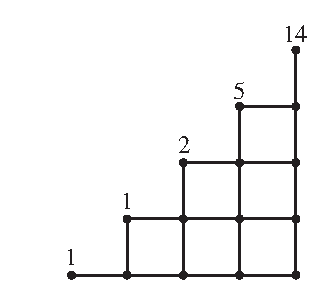
\includegraphics[width=0.33\linewidth]{images/CatalanPaths}
\caption{The lattice paths from \((0,0)\) to \((i,i)\) for \(i=0,1,2,3,4\).  The number of paths to the point \((i,i)\) is shown just above that point.\label{CatalanPaths}}
\end{figure}
~\par
\begin{enumerate}[label=(\alph*)]
 \item Explain why the number of lattice paths from \((0,0)\) to \((n,n)\) that go outside the triangle is the number of lattice paths from \((0,0)\) to \((n,n)\) that either touch or cross the line \(y=x+1\).%
\par\medskip\noindent%
\textbf{Solution.}\quad If a lattice path between \((0,0)\) and \((n,n)\) goes outside the triangle, it can only do so on an upstep. (A step from \((i,j)\) to \((i,j+1)\).) And an upstep must originate at a point with integer coordinates. If \(j\lt i\) an upstep from \((i,j))\) cannot leave the triangle. Thus to leave the triangle, the upstep must leave from a point of the form \((i,i)\), and go to \((i,i+1)\), which is on the line \(y=x+1\).%

~\par
\item Find a bijection between lattice paths from \((0,0)\) to \((n,n)\) that touch (or cross) the line \(y=x+1\) and lattice paths from \((-1,1)\) to \((n,n)\).%
\par\medskip\noindent%
\textbf{Solution.}\quad Suppose we have a lattice path form \((0,0)\) to \((n,n)\) which touches or crosses the line \(y=x+1\). Let \((k,k+1)\) be the first point on the line \(y=x+1\) that the lattice path touches. From that point, work backwards, replacing every upstep with a step one unit to the left and every rightstep with a step one unit down. The segment of the path you just changed will have moved left \(k+1\) times, so its leftmost \(x\) coordinate will be \(-1\), and it will have moved down \(k\) times, so its lowest \(y\) coordinate will be 1.  Thus we now have a lattice path from \((-1,1)\) to \((n,n)\). Further, given a lattice path from \((-1,1)\) to \((n,n)\), it must cross the line \(y=x+1\) at least once, because it starts above the line and ends below it. At the first point where such a path touches the line \(y=x+1\), say \((k',k'+1)\), work backwards replacing every upstep with a step to the left and every rightstep with a step downwards. The leftmost point on this path will have \(x\) coordinate 0, and the lowest point will have \(y\) coordinate 0, so the new path will be a lattice path from \((0,0)\) to \((n,n)\) that touches the line \(y=x+1\). Clearly these two processes reverse each other, and so they give us a bijection between paths form \((0,0)\) to \((n,n)\) that touch the line \(y=x+1\) and lattice lattice paths from \((-1,1)\) to \((n,n)\). Notice that geometrically what we are doing to get the bijection is to take the portion of a lattice path that goes from the initial point till the first touch of the line \(y=x+1\) and reflecting it around that line. This idea of reflection was introduced by Feller, and is called Feller's reflection principle.%

~\par
\item Find a formula for the number of lattice paths from \((0,0)\) to \((n,n)\) that do not cross the line \(y=x\).  The number of such paths is called a \emph{Catalan Number}\index{Catalan Number} and is usually denoted by \(C_n\).%
\par\medskip\noindent%
\textbf{Solution.}\quad \(C_n=\binom{2n}{n} - \binom{2n }{n+1}={1\over n+1}\binom{2n}{n}.\)%

\end{enumerate}
\end{activity}
\begin{activity}[]\label{activity-52}
Your formula for the Catalan Number can be expressed as a binomial coefficient divided by an integer. Whenever we have a formula that calls for division by an integer, an ideal combinatorial explanation of the formula is one that uses the quotient principle. The purpose of this problem is to find such an explanation using diagonal lattice paths.\footnote{The result we will derive is called the Chung-Feller Theorem\index{Chung-Feller Theorem}; this approach is based of a paper of Wen-jin Woan ``Uniform Partitions of Lattice Paths and Chung-Feller Generalizations," \textsl{American Mathematics Monthly 58} June/July 2001, p556.\label{fn-3}} A diagonal lattice path that never goes below the \(y\)-coordinate of its first point is called a \terminology{Dyck Path}\index{Dyck path}. We will call a Dyck Path from \((0,0)\) to \((2n,0)\) a \terminology{Catalan Path}\index{Catalan Path} of length \(2n\). Thus the number of Catalan Paths of length \(2n\) is the Catalan Number \(C_n\).%
~\par
\begin{enumerate}[label=(\alph*)]
 \item If a Dyck Path has \(n\) steps (each an upstep or downstep), why do the first \(k\) steps form a Dyck Path for each nonnegative \(k\le n\)?%
\par\medskip\noindent%
\textbf{Solution.}\quad If no points on the path are lower than the first point, then no points among the first \(k\) steps are lower than the first point.%

~\par
\item Thought of as a curve in the plane, a diagonal lattice path can have many local maxima and minima, and can have several absolute maxima and minima, that is, several highest points and several lowest points. What is the \(y\)-coordinate of an absolute minimum point of a Dyck Path starting at \((0,0)\)?  Explain why a Dyck Path whose rightmost absolute minimum point is its last point is a Catalan Path.%
\par\medskip\noindent%
\textbf{Solution.}\quad Since the path starts at \((0,0)\) and can't go below it, the \(y\) coordinate of an absolute minimum must be zero. If the last point is an absolute minimum, then (because it ends with the same \(y\) coordinate with which it starts) the path has an even number \(2k\) of steps and ends at \((2k,0)\).%

~\par
\item Let \(D\) be the set of all diagonal lattice paths from \((0,0)\) to \((2n,0)\).  (Thus these paths can go below the \(x\)-axis.) Suppose we partition \(D\) by letting \(B_i\) be the set of lattice paths in \(D\) that have \(i\) upsteps (perhaps mixed with some downsteps) following the last absolute minimum.  How many blocks does this partition have?  Give a succinct description of the block \(B_0\).%
\par\medskip\noindent%
\textbf{Solution.}\quad The path must have \(n\) upsteps total, and so can have any number between 0 and \(n\) upsteps after the rightmost absolute minimum. Thus the partition has \(n+1\) blocks. Block \(B_0\) consists of the Catalan Paths.%

~\par
\item How many upsteps are in a Catalan Path?%
\par\medskip\noindent%
\textbf{Solution.}\quad \(n\).%

~\par
\item We are going to give a bijection between the set of Catalan Paths and the block \(B_i\) for each \(i\) between \(1\) and \(n\).  For now, suppose the value of \(i\), while unknown, is fixed.  We take a Catalan path and break it into three pieces.  The piece \(F\) (for ``front'') consists of all steps before the \(i\)th upstep in the Catalan path.  The piece \(U\) (for ``up'') consists of the \(i\)th upstep.  The piece \(B\) (for ``back'') is the portion of the path that follows the \(i\)th upstep.  Thus we can think of the path as \(FUB\).  Show that the function that takes \(FUB\) to \(BUF\) is a bijection from the set of Catalan Paths onto the block \(B_i\) of the partition.  (Notice that \(BUF\) can go below the \(x\) axis.)%
\par\medskip\noindent%
\textbf{Solution.}\quad Since we are starting with a Catalan path, the point on the path at the beginning of the \(i\)th upstep must have \(y\) coordinate greater or equal to than zero. Thus wherever we start the sequence \(F\) of upsteps and downsteps, a path constructed by this sequence never goes lower than its starting point. Thus in \(BUF\) the last absolute minimum is either right before the \(U\) or earlier. But \(B\) is the final segment of a Catalan Path, so its final point is at least as low as its starting point. Thus the point at the beginning of the \(U\) in \(BUF\) is an absolute minimum, and there are \(i\) upsteps after that local minimum. If we take two different sequences and rearrange them in the same way, we get two different sequences, so the function we just described is a one-to-one function. If we take an arbitrary diagonal lattice path from \((0,0)\) to \((2n,0)\), let \(U'\) be the first upstep after the last absolute minimum, \(F'\) be the portion of the path that follows \(U'\), and \(B'\) be the portion that precedes \(U'\), then \(F'U'B'\) is a Catalan Path, and \(U'\) is its \(i\)th upstep if and only if in \(B'U'F'\) there are \(i\) upsteps after the last absolute minimum. Thus the mapping from \(FUB\) to \(BUF\) is a bijection.%

~\par
\item Explain how you have just given another proof of the formula for the Catalan Numbers.%
\par\medskip\noindent%
\textbf{Solution.}\quad We have taken the set of all \(\binom{2n}{n}\) diagonal lattice paths of length \(2n\) from \((0,0)\) to \((2n,0)\) and partitioned it into \(n+1\) blocks all of size \(C_n\). Thus by the quotient principle, \(C_n={1\over
n+1}\binom{2n
}{n}\).%

\end{enumerate}
\end{activity}
\typeout{************************************************}
\typeout{Subsection  The Binomial Theorem}
\typeout{************************************************}
\subsection[{The Binomial Theorem}]{The Binomial Theorem}\label{subsection-8}
\begin{activity}[]\label{Conjecturebinomthm}
We know that \((x+y)^2 = x^2+2xy+y^2\). Multiply both sides by \((x+y)\) to get a formula for \((x+y)^3\) and repeat to get a formula for \((x+y)^4\). Do you see a pattern? If so, what is it? If not, repeat the process to get a formula for \((x+y)^5\) and look back at \hyperref[Pascaltriangle]{Figure~\ref{Pascaltriangle}} to see the pattern. Conjecture a formula for \((x+y)^n\).%
\par\medskip\noindent%
\textbf{Solution.}\quad \((x+y)^3=x^3+2x^2y +xy^2+x^2y+ +2xy^2 +y^3=x^3+3x^2y++3xy^2+y^3\).%
\par
Similarly, \((x+4)^4=x^4+4x^3y+6x^2y^2+4xy^3+y^4\),%
\par
and \((x+y)^5=x^5+5x^4y+10x^3y^2+10x^2y^3+5xy^4+y^5.\) The pattern is that the coefficient of \(x^iy^j\) is \(\binom{i+j}{i}\) which is the same as \(\binom{i+j}{j}\). Said differently, the coefficient of \(x^{n-i}y^i\) is \(\binom{n}{i}\) or the coefficient of \(x^iy^{n-i}\) is \(\binom{n}{i}\). We conjecture that%
\begin{equation*}
(x+y)^n=\sum_{i=0}^n \binom{n}{i}x^{n-i}y^i.
\end{equation*}
%
\par
(The reason for putting \(x^{n-i}y^i\) into the sum is so that as \(i\) goes from 0 to \(n\), the powers of \(x\) decrease from \(n\) to 0.)%
\end{activity}
\begin{activity}[]\label{activity-54}
When we apply the distributive law \(n\) times to \((x+y)^n\), we get a sum of terms of the form \(x^iy^{n-i}\) for various values of the integer \(i\).%
~\par
\begin{enumerate}[label=(\alph*)]
 \item If it is clear to you that each term of the form \(x^iy^{n-i}\) that we get comes from choosing an \(x\) from \(i\) of the \((x+y)\) factors and a \(y\) from the remaining \(n-i\) of the factors and multiplying these choices together, then answer this part of the problem and skip the next part.  Otherwise, do the next part instead of this one.  In how many ways can we choose an \(x\) from \(i\) terms and a \(y\) from \(n-i\) terms?%
\par\medskip\noindent%
\textbf{Solution.}\quad The number of ways to choose an \(x\) from \(i\) of the factors and a \(y\) from the remaining ones is the way to choose the \(i\) factors from the \(n\) factors; that is, \(\binom{n}{i}\).%

~\par
\item Expand the product \((x_1 +y_1)(x_2 +y_2)(x_3+y_3)\).%
\par\medskip\noindent%
\textbf{Solution.}\quad %
\begin{align*}
(x_1+y_1)(x_2+y_2)(x_3+y_3)=x_1x_2x_3 \!\!\amp +\amp \!\!x_1x_2y_3+x_1y_2x_3+\\
y_1x_2x_3+x_1y_2y_3+y_1x_2y_3 \!\!\amp +\amp \!\! y_1y_2x_3+y_1y_2y_3.
\end{align*}
%

~\par
\item What do you get when you substitute \(x\) for each \(x_i\) and \(y\) for each \(y_i\)?%
\par\medskip\noindent%
\textbf{Solution.}\quad When you substitute \(x\) for each \(x_i\) and \(y\) for each \(y_i\), you get \((x+y)^3=x^3+3x^2y+3xy^2+y^3\).%

~\par
\item Now imagine expanding%
\begin{equation*}
(x_1+y_1)(x_2+y_2)\cdots (x_n+y_n).
\end{equation*}
Once you apply the commutative law to the individual terms you get, you will have a sum of terms of the form%
\begin{equation*}
x_{k_1}x_{k_2}\cdots x_{k_i}\cdot y_{j_1}y_{j_2}\cdots
y_{j_{n-i}}.
\end{equation*}
What is the set \(\{k_1,k_2,\ldots, k_i\}\cup \{j_1,j_2,\ldots, j_{n-i}\}\)?%
\par\medskip\noindent%
\textbf{Solution.}\quad \(\{k_1,k_2,\ldots, k_i\}\cup
\{j_1,j_2,\ldots, j_{n-i}\}=\{1,2,\ldots, n\}\).%

~\par
\item In how many ways can you choose the set \(\{k_1,k_2,\ldots, k_i\}\)?%
\par\medskip\noindent%
\textbf{Solution.}\quad You can choose the set \(\{k_1,k_2,\ldots k_i\}\) in \(\binom{n}{i}\) ways.%

~\par
\item Once you have chosen this set, how many choices do you have for \(\{j_1,j_2,\ldots, j_{n-i}\}\)?%
\par\medskip\noindent%
\textbf{Solution.}\quad Once you have chosen the set of \(k\)s, there is just one way to choose the set of \(j\)s.%

~\par
\item If you substitute \(x\) for each \(x_i\) and \(y\) for each \(y_i\), how many terms of the form \(x^iy^{n-i}\) will you have in the expanded product%
\begin{equation*}
(x_1+y_1)(x_2+y_2)\cdots (x_n+y_n)=(x+y)^n?
\end{equation*}
%
\par\medskip\noindent%
\textbf{Solution.}\quad If you substitute \(x\) for \(x_i\) and substitute \(y\) for \(y_i\), you will get \(\binom{n}{i}\) terms of the form \(x^iy^{n-i}\).%

~\par
\item How many terms of the form \(x^{n-i}y^i\) will you have?%
\par\medskip\noindent%
\textbf{Solution.}\quad You will also get \(\binom{n}{i}\) terms of the form \(x^{n-i}y^i\).%

~\par
\item Explain how you have just proved your conjecture from \hyperref[Conjecturebinomthm]{Problem~\ref{Conjecturebinomthm}}.  The theorem you have proved is called the \emph{Binomial Theorem}.\index{Binomial Theorem}%
\par\medskip\noindent%
\textbf{Solution.}\quad We have proved that the coefficient of \(x^iy^{n-i}\) in \((x+y)^n\) is \(\binom{n}{i}\), or equivalently that the coefficient of \(x^{n-i}y^i\) in \((x+y)^n\) is \(\binom{n}{i}\).%

\end{enumerate}
\end{activity}
\begin{activity}[]\label{activity-55}
What is \(\sum_{i=1}^n \binom{10}{i}3^i\)?%
\par\medskip\noindent%
\textbf{Solution.}\quad \(\sum_{i=1}^n \binom{10}{i}3^i=\sum_{i=0}^n
\binom{10}{i}3^i-\binom{10}{0}3^0 =(1+3)^{10}-1=4^{10}-1\)%
\end{activity}
\begin{activity}[]\label{activity-56}
What is \(\binom{n}{0}-\binom{n}{1}+\binom{n}{2}-\cdots \pm
\binom{n}{n}\) if \(n\) is an integer bigger than 0?%
\par\medskip\noindent%
\textbf{Solution.}\quad The sum is \(0\) because it is \((-1+1)^n\).%
\end{activity}
\begin{activity}[]\label{activity-57}
Explain why%
\begin{equation*}
\sum_{i=0}^m\binom{m}{i}\binom{n}{k-i} = \binom{m+n}{k}.
\end{equation*}
Find two different explanations.%
\par\medskip\noindent%
\textbf{Solution.}\quad When we expand both sides of \((x+y)^m(x+y)^n=(x+y)^{m+n}\) by the binomial theorem we get \(\sum_{i=0}^m\binom{m}{i}\binom{n}{k-i}\) as the coefficient of \(x^{m+n-k}y^k\) on the left hand side and \(\binom{m+n}{k}\) on the right hand side.%
\par
For a second explanation, to choose \(k\) elements out of the union of an \(m\)-element set and a disjoint \(n\)-element set, chose some number \(i\le m\) of them from the \(m\)-element set and the remaining \(k-i\) of them from the \(n\)-element set. The sum on the left hand side of the equation simply sums the number of such choices over all possible \(i\), and the binomial coefficient on the right hand side of the equation says we will end up choosing \(k\) elements from among our \(m+n\) elements.%
\end{activity}
\begin{activity}[]\label{activity-58}
From the symmetry of the binomial coefficients, it is not too hard to see that when \(n\) is an odd number, the number of subsets of \(\{1,2,\ldots,n\}\) of odd size equals the number of subsets of \(\{1,2,\ldots,n\}\) of even size. Is it true that when \(n\) is even the number of subsets of \(\{1,2,\ldots,n\}\) of even size equals the number of subsets of odd size? Why or why not?%
\par\medskip\noindent%
\textbf{Solution.}\quad It is true, because if \(n>0\), when you expand \((1-1)^n\) by the binomial theorem, you get an alternating sum of binomial coefficients equal to 0, and so the sum of the binomial coefficients \(\binom{n}{i}\) with \(i\) even must equal the sum of the binomial coefficients \(\binom{n}{i}\) with \(i\) odd.%
\end{activity}
\begin{activity}[]\label{activity-59}
What is \(\sum_{i=0}^n i\binom{n}{i}\)? (Hint: think about how you might use calculus.)%
\par\medskip\noindent%
\textbf{Solution.}\quad \(\sum_{i=0}^n(\binom{n}{i}x^i = (1+x)^n\). Taking derivatives of both sides gives us \(\sum_{i=0}^ni\binom{n}{i}x^{i-1} = n(1+x)^{n-1}.\). Now substitute 1 for \(x\) and you get \(\sum_{i=0}^n i\binom{n}{i} = n2^{n-1}\).%
\end{activity}
Notice how the proof you gave of the binomial theorem was a counting argument. It is interesting that an apparently algebraic theorem that tells us how to expand a power of a binomial is proved by an argument that amounts to counting the individual terms of the expansion. Part of the reason that combinatorial mathematics turns out to be so useful is that counting arguments often underlie important results of algebra. As the algebra becomes more sophisticated, so do the families of objects we have to count, but nonetheless we can develop a great deal of algebra on the basis of counting.%
\typeout{************************************************}
\typeout{Subsection  The pigeonhole principle}
\typeout{************************************************}
\subsection[{The pigeonhole principle}]{The pigeonhole principle}\label{subsection-9}
\begin{activity}[]\label{elevencoins}
American coins are all marked with the year in which they were made. How many coins do you need to have in your hand to guarantee that on two (at least) of them, the date has the same last digit? (When we say ``to guarantee that on two (at least) of them,\dots{}'' we mean that you can find two with the same last digit. You might be able to find three with that last digit, or you might be able to find one pair with the last digit 1 and one pair with the last digit 9, or any combination of equal last digits, as long as there is at least one pair with the same last digit.)%
\par\medskip\noindent%
\textbf{Solution.}\quad Since there are ten possible last digits, you need at least 11 coins, and with 11 coins, at least two last digits must be the same.%
\end{activity}
There are many ways in which you might explain your answer to \hyperref[elevencoins]{Activity~\ref{elevencoins}}. For example, you can partition the coins according to the last digit of their date; that is, you put all the coins with a given last digit in a block together, and put no other coins in that block; repeating until all coins are in some block. Then you have a partition of your set of coins. If no two coins have the same last digit, then each block has exactly one coin. Since there are only ten digits, there are at most ten blocks and so by the sum principle there are at most ten coins. In fact with ten coins it is possible to have no two with the same last digit, but with 11 coins some block must have at least two coins in order for the sum of the sizes of at most ten blocks to be 11. This is one explanation of why we need 11 coins in \hyperref[elevencoins]{Activity~\ref{elevencoins}}. This kind of situation arises often in combinatorial situations, and so rather than always using the sum principle to explain our reasoning , we enunciate another principle which we can think of as yet another variant of the sum principle. The \terminology{pigeonhole principle}\index{pigeonhole principle} states that%
\begin{quote}If we partition a set with more than \(n\) elements into \(n\) parts, then at least one part has more than one element.%
\end{quote}
The pigeonhole principle gets its name from the idea of a grid of little boxes that might be used, for example, to sort mail, or as mailboxes for a group of people in an office. The boxes in such grids are sometimes called pigeonholes in analogy with stacks of boxes used to house homing pigeons when homing pigeons were used to carry messages. People will sometimes state the principle in a more colorful way as ``if we put more than \(n\) pigeons into \(n\) pigeonholes, then some pigeonhole has more than one pigeon.''%
\begin{activity}[]\label{activity-61}
Show that if we have a function from a set of size \(n\) to a set of size less than \(n\), then \(f\) is not one-to-one.%
\par\medskip\noindent%
\textbf{Solution.}\quad Let \(T\) be the set of size less than \(n\), and \(S\) be the set of size \(n\). Let \(B_j=\{i|f(i)=j\}\) for each \(j\) in \(T\). Then the nonempty sets among the \(B_j\)s form a partition of \(S\) and the number of blocks is less than the size of \(S\). Therefore by the pigeonhole principle, there is at least one block with at least two elements, so there are two elements \(i_1\) and \(i_2\) such that \(f(i_1)=f(i_2)\).%
\end{activity}
\begin{activity}[]\label{activity-62}
Show that if \(S\) and \(T\) are finite sets of the same size, then a function \(f\) from \(S\) to \(T\) is one-to-one if and only if it is onto.%
\par\medskip\noindent%
\textbf{Solution.}\quad First suppose that \(f\) is a one-to-one function from \(S\) to \(T\), sets which have the same size. Let \(B_j=\{i|f(i)=j\}\) for each \(j\) in \(T\)..  If \(f\) is not onto, then the number of nonempty sets \(B_j\) is smaller than the number of elements of \(T\) and thus is smaller than the size of \(S\). The nonempty sets \(B_j\) are a partition of \(S\). But then by the pigeonhole principle, some nonempty \(B_j\) has two or more elements, contradicting the assumption that \(f\) is one-to-one. Therefore if \(f\) is one-to-one, then it is onto. Now suppose that \(f\) is an onto function from \(S\) to \(T\), sets of the same size. Again let \(B_j =\{i|f(i)=j\}\) for each \(j\) in \(T\). The size of the union of the sets \(B_j\) is, by the sum principle, the sum of their sizes. Since \(f\) is onto, each \(B_j\) has at least one element. Since the number of sets \(B_j\) is the number of elements of \(S\), if one of those sets has more than one element, the the size of their union is more than the size of \(S\), which is a contradiction since they are subsets of \(S\). Therefore each set \(B_j\) has exactly one element and therefore \(f\) is one-to-one.%
\end{activity}
\begin{activity}[]\label{activity-63}
There is a \terminology{generalized pigeonhole principle}\index{pigeonhole principle!generalized} which says that if we partition a set with more than \(kn\) elements into \(n\) blocks, then at least one block has at least \(k+1\) elements. Prove the generalized pigeonhole principle.%
\par\medskip\noindent%
\textbf{Solution.}\quad Suppose we partition a set \(S\) of more than \(kn\) elements into \(n\) blocks. If each block has at most \(k\) elements, the by the sum principle the size of \(S\) is at most \(kn\). But this is a contradiction, so some block has at least \(k+1\) elements.%
\end{activity}
\begin{activity}[]\label{activity-64}
All the powers of five end in a five, and all the powers of two are even. Show that for for some integer \(n\), if you take the first \(n\) powers of a prime other than two or five, one must have ``01'' as the last two digits.%
\par\medskip\noindent%
\textbf{Solution.}\quad If we take 40 powers of such a prime, either one will end in ``01'' or some two, say \(p^i\) and \(p^j\) with \(i>j\) must have the same last two digits by the pigeon hole principle. Then \(p^i-p^j=100k\) for some integer \(k\). Thus \(p^j(p^{i-j} -1)\) must be a multiple of 100, and since neither 2 nor 5 divide \(p\), \(p^{i-j} -1 = 100k'\) for some integer \(k'\) then \(p^{i-j} = 100k'+1\), so the last two digits of \(p^{i-j}\) must be ``01.''%
\end{activity}
\begin{activity}[]\label{R_3_3_}
Show that in a set of six people, there is a set of at least three people who all know each other, or a set of at least three people none of whom know each other. (We assume that if person 1 knows person 2, then person 2 knows person 1.)%
\par\medskip\noindent%
\textbf{Solution.}\quad By the generalized pigeonhole principle, person 1 either knows at least three people or doesn't know at least three people. Suppose person 1 knows three people. Then either two of these people know each other, giving us, with person 1, three mutual acquaintances, or no two of these people know each other, giving us three mutual strangers. On the other hand if there are three people person 1 does not know, then either two of these people don't know each other, giving us, with person 1, three mutual strangers, or all three of these people know each other, giving us three mutual acquaintances.%
\end{activity}
\begin{activity}[]\label{notR_3_3_}
Draw five circles labeled Al, Sue, Don, Pam, and Jo. Find a way to draw red and green lines between people so that every pair of people is joined by a line and there is neither a triangle consisting entirely of red lines or a triangle consisting of green lines. What does \hyperref[R_3_3_]{Problem~\ref{R_3_3_}} tell you about the possibility of doing this with six people's names? What does this problem say about the conclusion of \hyperref[R_3_3_]{Problem~\ref{R_3_3_}} holding when there are five people in our set rather than six?%
\par\medskip\noindent%
\textbf{Solution.}\quad In the figure that follows, we use solid lines for red and dashed lines for green. Clearly there is no solid triangle and no dashed triangle.%
\begin{figure}
\centering
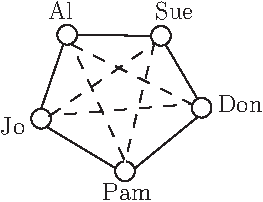
\includegraphics[width=0.33\linewidth]{images/NonRamsey5}
\end{figure}
\hyperref[R_3_3_]{Activity~\ref{R_3_3_}} says you can't do this with six people's names. This problem says that the conclusion of \hyperref[R_3_3_]{Activity~\ref{R_3_3_}} does not hold when you have five people.%
\end{activity}
\typeout{************************************************}
\typeout{Subsection  Ramsey Numbers}
\typeout{************************************************}
\subsection[{Ramsey Numbers}]{Ramsey Numbers}\label{Ramseysection}
Activity~\hyperref[R_3_3_]{\ref{R_3_3_}}--\hyperref[notR_3_3_]{\ref{notR_3_3_}} together show that six is the smallest number \(R\) with the property that if we have \(R\) people in a room, then there is either a set of (at least) three mutual acquaintances or a set of (at least) three mutual strangers. Another way to say the same thing is to say that six is the smallest number so that no matter how we connect 6 points in the plane (no three on a line) with red and green lines, we can find either a red triangle or a green triangle. There is a name for this property. The \terminology{Ramsey Number} \(R(m,n)\) is the smallest number \(R\) so that if we have \(R\) people in a room, then there is a set of at least \(m\) mutual acquaintances or at least \(n\) mutual strangers. There is also a geometric description of Ramsey Numbers; it uses the idea of a \emph{complete graph} on \(R\) vertices. A \emph{complete graph}\index{graph!complete} on \(R\) vertices consists of \(R\) points in the plane together with line segments (or curves) connecting each two of the \(R\) vertices.\footnote{As you may have guessed, a complete graph is a special case of something called a graph.  The word graph will be defined in \hyperref[graphsection]{Subsection~}.\label{fn-4}} The points are called \terminology{vertices}\index{vertex!of a complete graph}\index{vertex} and the line segments are called \terminology{edges}\index{edge!of a complete graph}\index{edge}. In \hyperref[completegraph]{Figure~\ref{completegraph}} we show three different ways to draw a complete graph on four vertices. We use \(K_n\) to stand for a complete graph on \(n\) vertices.%
\begin{figure}
\centering
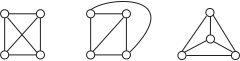
\includegraphics[width=0.33\linewidth]{images/threeK4s}
\caption{Three ways to draw a complete graph on four vertices\label{completegraph}}
\end{figure}
Our geometric description of \(R(3,3)\) may be translated into the language of graph theory (which is the subject that includes complete graphs) by saying \(R(3,3)\) is the smallest number \(R\) so that if we color the edges of a \(K_R\) with two colors, then we can find in our picture a \(K_3\) all of whose edges have the same color.  The graph theory description of \(R(m,n)\) is that \(R(m,n)\) is the smallest number \(R\) so that if we color the edges of a \(K_R\) with red and green, then we can find in our picture either a \(K_m\) all of whose edges are red or a \(K_n\) all of whose edges are green. Because we could have said our colors in the opposite order, we may conclude that \(R(m,n) = R(n,m)\). In particular \(R(n,n)\) is the smallest number \(R\) such that if we color the edges of a \(K_R\) with two colors, then our picture contains a \(K_n\) all of whose edges have the same color.%
\begin{activity}[]\label{activity-67}
Since \(R(3,3)=6\), an uneducated guess might be that \(R(4,4)=8\). Show that this is not the case.%
\par\medskip\noindent%
\textbf{Solution.}\quad In the graph of \hyperref[NonRamsey8]{Figure~\ref{NonRamsey8}}, each vertex has three dashed lines emanating from it, and there are no dashed lines connecting any of the three vertices adjacent to it by dashed lines. Each vertex has four solid lines emanating from it, and no three of the four vertices adjacent to it by solid lines are all adjacent by solid lines. Thus there is no solid line \(K_4\) and there is no dashed line \(K_4\).%
\begin{figure}
\centering
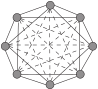
\includegraphics[width=0.33\linewidth]{images/NonRamsey8}
\caption{A graph showing \(R(4,4) \gt 8\)\label{NonRamsey8}}
\end{figure}
\end{activity}
\begin{activity}[]\label{activity-68}
Show that among ten people, there are either four mutual acquaintances or three mutual strangers. What does this say about \(R(4,3)\)?%
\par\medskip\noindent%
\textbf{Solution.}\quad Take a person, say person 1. If person has six acquaintances, then by \hyperref[R_3_3_]{Activity~\ref{R_3_3_}} among them there are either three mutual strangers, in which case we are done, or three mutual acquaintances. These three acquaintances together with person 1 form a set of 4 mutual acquaintances in which case we are again done. Thus we may assume Person 1 has at most 5 acquaintances, and so has four non-acquaintances. Now either all four of these people are acquainted, in which case we are done, or else two of them are not acquainted. Then these two people, together with person 1 make three mutual nonacquaintances. Therefore in every possible case, we have either four mutual acquaintances or three mutual strangers. This means that \(R(4,3) \le 10\).%
\end{activity}
\begin{activity}[]\label{OddNoPeople}
Show that among an odd number of people there is at least one person who is an acquaintance of an even number of people and therefore also a stranger to an even number of people.%
\par\medskip\noindent%
\textbf{Solution.}\quad Suppose we add, for each person, the number of people with whom he or she is acquainted. Then we get twice the number of acquaintance edges in the graph of acquaintance and non-acquaintance relationships. Thus the sum must be even. But if each person among an odd number of people were acquainted with an odd number of people, then the sum would be odd. Since this is a contradiction, among an odd number of people, there must be at least one who is acquainted with an even number of people. Since the number of people different from this person is even, the number of people with whom this person is not acquainted is also even.%
\end{activity}
\begin{activity}[]\label{R_4_3_not8}
Find a way to color the edges of a \(K_8\) with red and green so that there is no red \(K_4\) and no green \(K_3\).%
\par\medskip\noindent%
\textbf{Solution.}\quad In the graph shown in \hyperref[NonRamsey8]{Figure~\ref{NonRamsey8}}, there is no \(K_3\) whose edges are dashed, and no \(K_4\) whose edges are solid. By symmetry, to verify this you need only look at vertex 1 and vertices connected to it by either dashed lines or by solid lines.%
\end{activity}
\begin{activity}[]\label{activity-71}
Find \(R(4,3)\).%
\par\medskip\noindent%
\textbf{Solution.}\quad \(R(4,3)=9\). In \hyperref[R_4_3_not8]{Activity~\ref{R_4_3_not8}} we showed that \(R(4,3)\) is more than 8. So we must show that if we have nine people, we either have 4 mutual acquaintances or three mutual strangers. By \hyperref[OddNoPeople]{Activity~\ref{OddNoPeople}} there is at least one person (say person A) who is acquainted with an even number of people. If person A is acquainted with six or more people, then among these six people, there are either three mutual acquaintances or three mutual strangers. If there are three mutual strangers, we are done; if there are three mutual acquaintances, they, together with Person A are four mutual acquaintances. Thus we may assume Person A is acquainted with at most four people. Thus person A is a stranger to at least four people. If two of these people are strangers, then they, together with person A form three mutual strangers and we are done. Otherwise all of these people know each other and we have at least four mutual acquaintances, and so in every possible situation, we have either four mutual acquaintances or three mutual strangers.%
\end{activity}
As of this writing, relatively few Ramsey Numbers are known. \(R(3,n)\) is known for \(n\lt 10\), \(R(4,4) = 18\), and \(R(5,4)=R(4,5)=25\).%
\typeout{************************************************}
\typeout{Section 0.4 Supplementary Chapter Problems}
\typeout{************************************************}
\section[{Supplementary Chapter Problems}]{Supplementary Chapter Problems}\label{section-4}
\leavevmode%
\begin{enumerate}
\item\hypertarget{compositiondefinition}{}(interesting) Remember that we can write \(n\) as a sum of \(n\) ones.  How many plus signs do we use?  In how many ways may we write \(n\) as a sum of a list of \(k\) positive numbers?  Such a list is called a \emph{composition}\index{composition} of \(n\) into \(k\) parts.\index{composition!\(k\) parts}\index{composition!\(k\) parts!number of} We use \(n-1\) plus signs. Write down such a sum and choose \(k-1\) of the plus signs. Then each string of ones and plusses between two chosen plus signs, before the first chosen plus sign or after the last chosen one corresponds to a part of a composition of \(n\). Thus the number of compositions of \(n\) with \(k\) parts is the number of ways to choose the \(k-1\) places, which is \(\binom{n-1}{k-1}\).%
%
\item\hypertarget{composition_numberof}{}In \hyperlink{compositiondefinition}{Problem~1} we defined a composition of \(n\) into \(k\) parts.  What is the total number of compositions of \(n\) (into any number of parts). \index{compositions!number of} The total number of compositions is the number of ways to choose a subset of the plus signs which is \(2^{n-1}\).%
%
\item\hypertarget{GreyCode}{}(essential for this or the next section) Write down a list of all 16 0-1 sequences of length four starting with 0000 in such a way that each entry differs from the precious one by changing just one digit.  This is called a Grey Code.\index{Grey Code}  That is, a \emph{Grey Code} for 0-1 sequences of length \(n\) is a list of the sequences so that each entry differs from the previous one in exactly one place.  Can you describe how to get a Grey Code for 0-1 sequences of length five from the one you found for sequences of length 4?  Can you describe how to prove that there is a Grey code for sequences of length \(n\)? (One of many) 0000, 0001, 0011, 0010, 0110, 0111, 0101, 0100, 1100, 1101, 1111, 1110, 1010, 1011, 1001, 1000. To get a code for sequences of length 5, put a zero at the end of each of the sequences we have. Follow that revised sequence by 10001, and write the remainder of the sequence in reverse order with a 1 at the end of each term. (Don't reverse the individual length four sequences, just the sequence of sequences!) We just, in essence, described the inductive step of an inductive proof that Grey Codes exist for sequences of any length.%
%
\item\hypertarget{li-12}{}(interesting) Use the idea of a Grey Code from \hyperlink{GreyCode}{Problem~3} to prove bijectively that the number of even-sized subsets of an \(n\)-element set equals the number of odd-sized subsets of an \(n\)-element set. Each sequence in the Grey Code is the characteristic function of a set, and the number of elements of the set is the number of ones in the sequence. Since each sequence differs in just one place from the preceding one, the sequences alternate between having an even number of ones and an odd number of ones. Since the first sequence is all zeros and there are \(2^n\) sequences, the last one has an odd number of zeros. Thus the map that takes each sequence except the last to the next one, and takes the last to the first is a bijection between the characteristic functions of sets with an even number of elements and sets with an odd number of elements.%
%
\item\hypertarget{li-13}{}(interesting) A list of parentheses is said to be balanced if there are the same number of left parentheses as right, and as we count from left to right we always find at least as many left parentheses as right parentheses.  For example, (((()()))()) is balanced and ((()) and (()()))(() are not.  How many balanced lists of \(n\) left and \(n\)  right parentheses are there? The number is the Catalan number: we get a bijection between balanced lists of parentheses and Catalan paths by sending each left paren to an upstep and each right paren to a downstep. The condition that there are always as many left parentheses as right ensures we never go below the \(x\) axis.%
%
\item\hypertarget{li-14}{}(difficult) Suppose we plan to put six distinct computers in a network as shown in \hyperref[hexagonalnetwork]{Figure~\ref{hexagonalnetwork}}.  The lines show which computers can communicate directly with which others.  Consider two ways of assigning computers to the nodes of the network different if there are two computers that communicate directly in one assignment and that don't communicate directly in the other.  In how many different ways can we assign computers to the network? \begin{figure}
\centering
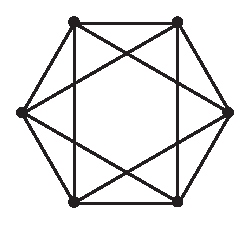
\includegraphics[width=0.33\linewidth]{images/HexagonalNetwork}
\caption{A computer network.\label{hexagonalnetwork}}
\end{figure}
 We consider two assignments of computers to be equivalent if in both assignments, each computer communicates directly with exactly the same computers. This partitions the set of all \(6!\) computer assignments into blocks of \(48\) computers each. Thus we have \(720/48=15\) ways to assign the computers to the network.%
%
\item\hypertarget{li-15}{}(interesting) In a circular ice cream dish we are going to put four distinct scoops of ice cream chosen from among twelve flavors.  Assuming we place four scoops of the same size as if they were at the corners of a square, and recognizing that moving the dish doesn't change the way in which we have put the ice cream into the dish, in how many ways may we choose the ice cream and put it into the dish? Each ice cream arrangement is equivalent to three others, the ones we get by rotating the dish. This divides the arrangements of four flavors of ice cream into blocks of size 4. Thus we may arrange the ice cream we have chosen in the dish in \(4!/4=6\) ways. We may choose the ice cream in \(\binom{12}{4}=495\) ways, and so we may choose it and put it into the dish in 2970 ways.%
%
\item\hypertarget{li-16}{}(interesting) In as many ways as you can, show that \(\binom{n}{k}\binom{n-k}{m} =
\binom{n}{m}\binom{n-m}{k}\). You can prove this by plugging in the formula for \(\binom{n}{k}\) on both sides and cancelling stuff until you get the same thing on both sides. However a much more interesting proof is that the right hand side counts the number of ways to choose a \(k\)-element set form an \(n\)-element set and then choose an \(m\)-element set from what remains. The left hand side counts the number of ways to first chose a \(k\)-element subset from the \(n\)-element set and then choose an \(m\)-element subset from what remains. Thus in both cases you are counting the number of ways to choose an ordered pair consisting of an \(m\)-element subset and a disjoint \(k\)-element subset from an \(n\)-element set. You can also base a proof on the observation that \((x+y+x)^n=
\sum_{k=0}^n\binom{n}{k}(x+y)^kz^{n-k}\) and \((x+y+z)^n=\sum_{m=0}^n\binom{n}{m}x^m(y+z)^{n-m}\) and asking for the coefficient of \(x^my^{n-m-k}z^k\). You do have to use the binomial theorem with an eye to the result you are looking for, however.%
%
\item\hypertarget{li-17}{}(interesting) A tennis club has \(4n\) members.  To specify a doubles match, we choose two teams of two people.  In how many ways may we arrange the members into doubles matches so that each player is in one doubles match?  In how many ways may we do it if we specify in addition who serves first on each team? We now have many methods for solving this problem. Perhaps the easiest is to list all \((4n)\) people and take them in groups of four for doubles matches, with the first two in a group of four as one team and the second two as another team. We note that interchanging the \(n\) blocks of 4 does not change the matches, nor does interchanging the two people on a team nor interchanging the two teams. Thus we have \((4n)!/n!2^{3n}\) ways to arrange the matches. If we are to say who serves first on each team, we might as well say it is the first of the two listed, so now we have \((4n)!/n!2^n\) ways to arrange the matches.%
%
\item\hypertarget{li-18}{}A town has \(n\) streetlights running along the north side of main street.  The poles on which they are mounted need to be painted so that they do not rust.  In how many ways may they be painted with red, white, blue, and green if an even number of them are to be painted green? We can think of first choosing the set of even size of poles to be painted green, and the painting the remaining poles red, white, and blue. We may do this in \(\sum_{k=0}^{\lfloor n/2\rfloor}\binom{n}{2k}3^{n-2k}\) ways.%
%
\item\hypertarget{pingpongpaint}{}We have \(n\) identical ping-pong balls.  In how many ways may we paint them red, white, blue, and green? We can line up the identical ping-pong balls and break them into four groups, those of each color, by inserting dividers. If we want to paint at least one in each color, we can choose three of the spaces between the balls in which to insert dividers, so we can paint them in \(\binom{n-1}{k}\). But the problem didn't require us to use each color, so we can put two dividers adjacent to each other. Thus there are \(n+1\) places where we can put the first divider (putting it before all the balls means we use no red, and putting it after all of them means we use no green. Now there are \(n+2\) places where we can put the second divider, including before or after the first, and \(n+3\) places where we can put the third divider. However if we interchange two dividers we still paint the balls before the first divider red, those between then next two white, and so on. Thus \(3!=6\) of these arrangements of balls and dividers correspond to the same paint job, so the number of ways to paint the balls is \({(n+1)(n+2)(n+3)\over6} =\binom{n+3}{3}\). This suggests that another way to think of the problem is to consider \(n+3\) slots in a row, and fill \(n\) of them with balls and \(3\) of them with dividers; since the balls are identical and the dividers might as well be identical, the number of ways to do this is the number of ways to choose the slots that get dividers.%
%
\item\hypertarget{li-20}{}We have \(n\) identical ping-pong balls.  In how many ways may we paint them red, white, blue, and green if we use green paint on an even number of them? We first decide how many balls to paint green, then paint the remainder with the other three colors as in \hyperlink{pingpongpaint}{Problem~11} This gives us%
\begin{equation*}
\sum_{k=0}^{\lfloor n/2\rfloor}\binom{n-2k+2}{2}
\end{equation*}
ways to paint the balls.%
%
\end{enumerate}
\typeout{************************************************}
\typeout{Chapter 1 Applications of Induction and Recursion in Combinatorics and Graph Theory}
\typeout{************************************************}
\chapter[{Applications of Induction and Recursion in Combinatorics and Graph Theory}]{Applications of Induction and Recursion in Combinatorics and Graph Theory}\label{InductionRecursion}
\typeout{************************************************}
\typeout{Section 1.1 Some Examples of Mathematical Induction}
\typeout{************************************************}
\section[{Some Examples of Mathematical Induction}]{Some Examples of Mathematical Induction}\label{sec_induction-examples}
\typeout{************************************************}
\typeout{Introduction  }
\typeout{************************************************}
In Chapter 1 ({$\langle\langle$Unresolved xref, reference "SubsetsByInduction"; check spelling or use "provisional" attribute$\rangle\rangle$}), we used the principle of mathematical induction to prove that a set of size \(n\) has \(2^n\) subsets. If you were unable to do that problem and you haven't yet read \hyperref[Induction]{Appendix~\ref{Induction}} (a portion of which is repeated here), you should do so now.%
\typeout{************************************************}
\typeout{Subsection  Mathematical induction}
\typeout{************************************************}
\subsection[{Mathematical induction}]{Mathematical induction}\label{subsection-11}
\typeout{************************************************}
\typeout{Introduction  }
\typeout{************************************************}
The \emph{principle of mathematical induction}\index{mathematical induction!principle of}\index{principle of mathematical induction}\index{induction!mathematical, the principle of} states that%
\begin{quote}In order to prove a statement about an integer \(n\), if we can \leavevmode%
\begin{enumerate}
\item\hypertarget{li-21}{}Prove the statement when \(n=b\), for some fixed integer \(b\)%
\item\hypertarget{li-22}{}Show that the truth of the statement for \(n=k-1\) implies the truth of the statement for \(n=k\) whenever \(k>b\),%
\end{enumerate}
 then we can conclude the statement is true for all integers \(n\ge
b\).\end{quote}
As an example, let us return to {$\langle\langle$Unresolved xref, reference "SubsetsByInduction"; check spelling or use "provisional" attribute$\rangle\rangle$}. The statement we wish to prove is the statement that ``A set of size \(n\) has \(2^n\) subsets.''%
\begin{quote}Our statement is true when \(n=0\), because a set of size 0 is the empty set and the empty set has \(1=2^0\) subsets. (This step of our proof is called a \emph{base step}.) Now suppose that \(k>0\) and every set with \(k-1\) elements has \(2^{k-1}\) subsets.  Suppose \(S=\{a_1,a_2,\ldots a_k\}\) is a set with \(k\) elements. We partition the subsets of \(S\) into two blocks.  Block \(B_1\) consists of the subsets that do not contain \(a_n\) and block \(B_2\) consists of the subsets that do contain \(a_n\).  Each set in \(B_1\) is a subset of \(\{a_1,a_2,\ldots a_{k-1}\}\), and each subset of \(\{a_1,a_2, \ldots
a_{k-1}\}\) is in \(B_1\).  Thus \(B_1\) is the set of all subsets of \(\{a_1,a_2,\ldots a_{k-1}\}\).  Therefore by our assumption in the first sentence of this paragraph, the size of \(B_1\) is \(2^{k-1}\).  Consider the function from \(B_2\) to \(B_1\) which takes a subset of \(S\) including \(a_k\) and removes \(a_k\) from it.  This function is defined on \(B_2\), because every set in \(B_2\) contains \(a_k\).  This function is onto, because if \(T\) is a set in \(B_1\), then \(T\cup \{a_k\}\) is a set in \(B_2\) which the function sends to \(T\).  This function is one-to-one because if \(V\) and \(W\) are two different sets in \(B_2\), then removing \(a_k\) from them gives two different sets in \(B_1\).  Thus we have a bijection between \(B_1\) and \(B_2\), so \(B_1\) and \(B_2\) have the same size.  Therefore by the sum principle the size of \(B_1\cup B_2\) is \(2^{k-1} +2^{k-1}=2^k\).  Therefore \(S\) has \(2^k\) subsets.  This shows that if a set of size \(k-1\) has \(2^{k-1}\) subsets, then a set of size \(k\) has \(2^k\) subsets.  Therefore by the principle of mathematical induction, a set of size \(n\) has \(2^n\) subsets for every nonnegative integer \(n\).\end{quote}
The first sentence of the last paragraph is called the \emph{inductive hypothesis}. In an inductive proof we always make an inductive hypothesis as part of proving that the truth of our statement when \(n=k-1\) implies the truth of our statement when \(n=k\). The last paragraph itself is called the \emph{inductive step} of our proof. In an inductive step we derive the statement for \(n=k\) from the statement for \(n=k-1\), thus proving that the truth of our statement when \(n=k-1\) implies the truth of our statement when \(n=k\). The last sentence in the last paragraph is called the \emph{inductive conclusion}. All inductive proofs should have a base step, an inductive hypothesis, an inductive step, and an inductive conclusion.%
\par
There are a couple details worth noticing. First, in this problem, our base step was the case \(n=0\), or in other words, we had \(b=0\). However, in other proofs, \(b\) could be any integer, positive, negative, or 0. Second, our proof that the truth of our statement for \(n=k-1\) implies the truth of our statement for \(n=k\) required that \(k\) be at least 1, so that there would be an element \(a_k\) we could take away in order to describe our bijection. However, condition (2) of the principle of mathematical induction only requires that we be able to prove the implication for \(k>0\), so we were allowed to assume \(k>0\).%
\typeout{************************************************}
\typeout{Subsubsection  Strong Mathematical Induction}
\typeout{************************************************}
\subsubsection[{Strong Mathematical Induction}]{Strong Mathematical Induction}\label{subsubsection-1}
One way of looking at the principle of mathematical induction is that it tells us that if we know the ``first'' case of a theorem and we can derive each other case of the theorem from a smaller case, then the theorem is true in all cases. However the particular way in which we stated the theorem is rather restrictive in that it requires us to derive each case from the immediately preceding case. This restriction is not necessary, and removing it leads us to a more general statement of the principal of mathematical induction which people often call the \emph{strong principle of mathematical induction}. It states:%
\begin{quote}In order to prove a statement about an integer \(n\) if we can \leavevmode%
\begin{enumerate}
\item\hypertarget{li-23}{}prove our statement when \(n=b\) and%
\item\hypertarget{li-24}{}prove that the statements we get with \(n=b\), \(n=b+1\), \dots{} \(n=k-1\) imply the statement with \(n=k\),%
\end{enumerate}
 then our statement is true for all integers \(n\ge b\).\end{quote}
You will find some explicit examples of the use of the strong principle of mathematical induction in \hyperref[Induction]{Appendix~\ref{Induction}} and will find some uses for it in this chapter.%
\typeout{************************************************}
\typeout{Subsection  Binomial Coefficients and the Binomial Theorem}
\typeout{************************************************}
\subsection[{Binomial Coefficients and the Binomial Theorem}]{Binomial Coefficients and the Binomial Theorem}\label{subsection-12}
\begin{activity}[]\label{activity-72}
When we studied the Pascal Equation and subsets in Chapter 1, it may have appeared that there is no connection between the Pascal relation \(\binom{n}{k} = \binom{n-1}{k-1} +\binom{n-1}{k}\) and the formula \(\binom{n}{k}={n!\over k!(n-k)!}\). Of course you probably realize you can prove the Pascal relation by substituting the values the formula gives you into the right-hand side of the equation and simplifying to give you the left hand side. In fact, from the Pascal Relation and the facts that \(\binom{n}{0}=1\) and \(\binom{n}{n}=1\), you can actually prove the formula for \(\binom{n}{k}\) by induction on \(n\). Do so.%
\par\medskip\noindent%
\textbf{Solution.}\quad We wish to prove that \(\binom{n}{i} ={n!\over i!(n-i)!}\). We note that since \(\binom{n}{0}=1\) and \(\binom{n}{n} =1\) are in agreement with this formula, we only have to consider the cases in which \(0\lt i\lt n\), which by the way, requires that \(n\ge 2\). We will prove that our formula holds by induction on \(n\) for \(n\ge 2\). If \(n=2\), the only \(i\) we need to consider is \(i=1\), and we know that \(\binom{2}{1}=2\), the number of one-element subsets of a two-element set. But \(2!\over1!(2-1)!\) is 2 also, so our formula holds when \(n=2\). Now suppose our formula holds when \(n=k-1\), so that for every \(i\) with \(0\lt i\lt n-1\), \(\binom{k-1}{i} =
{(k-1)!\over i!(k-1-i)!}\). Then by the Pascal Equation%
\begin{align*}
\binom{k}{i}\amp =\amp \binom{k-1}{i-1}+\binom{k-1}{i}\\
\amp =\amp
{(k-1)!\over (i-1)!(k-1-i+1)!} + {(k-1)!\over
i!(k-1-i)!}\\
\amp =\amp {(k-1)!i+(k-1)!(k-i)\over i!(k-i)!} \ =\  {k!\over
i!(k-i)!}.
\end{align*}
%
\par
Thus the truth of our formula for \(n=k-1\) implies its truth for \(n=k\). Therefore by the principle of mathematical induction, our formula is true for all integers \(n\ge 2\). We have already seen is is true when \(i=0\) or \(i=1\), so it is true for all nonnegative \(n\) and all numbers \(i\) with \(0\le i\le n\).%
\end{activity}
\begin{activity}[]\label{activity-73}
~\par
\begin{enumerate}[label=(\alph*)]
 \item Use the fact that \((x+y)^n = (x+y)(x+y)^{n-1}\) to give an inductive proof of the binomial theorem.%
\par\medskip\noindent%
\textbf{Solution.}\quad We prove the binomial theorem by induction on \(n\). When \(n=0\), \((x+y)^n=(x+y)^0=1=\sum_{i=0}^0 \binom{n}{i}x^{0-i}y^i\) since that last summation consists of the one term \(\binom{0}{0}x^0y^0\).%
\par
Now suppose that when \(n=k-1\), \((x+y)^n=\sum_{i=0}^n \binom{n}{i}x^{n-i}y^i.\) This gives us%
\begin{align*}
(x+y)^k\amp =\amp (x+y)(x+y)^{k-1}=(x+y)\sum_{i=0}^{k-1}\binom{k-1}{i}x^{k-1-i}y^i\\
\amp =\amp \sum_{i=0}^{k-1}\binom{k-1}{i}x^{k-i}y^i+\sum_{i=0}^{k-1} \binom{k-1}{i}x^{k-1-i}y^{i+1}\\
\amp =\amp \sum_{i=0}^{k-1}\binom{k-1}{i}x^{k-i}y^i+\sum_{i=1}^{k} \binom{k-1}{i-1}x^{k-i}y^{i}\\
\amp =\amp  x^k+\left(\sum_{i=1}^{k-1}\binom{k-1}{i}x^{k-i}y^i+\binom{k-1}{i-1}x^{k-i}y^i\right) +y^k\\
\amp =\amp  x^k+\left(\sum_{i=1}^{k-1} \binom{k}{i}x^{k-i}y^i\right) +y^k\ =\
\sum_{i=0}^k \binom{k}{i}x^{k-i}y^i.
\end{align*}
%
\par
Thus the truth of the binomial theorem for \(n=k-1\) implies its truth for \(n=k\). Then by the principle of mathematical induction, the binomial theorem must be true for all integers \(n\ge 0\).%

~\par
\item Suppose that \(f\) is a function defined on the nonnegative integers such that \(f(0)=3\) and \(f(n)=2f(n-1)\). Find a formula for \(f(n)\) and prove your formula is correct.%
\par\medskip\noindent%
\textbf{Solution.}\quad \(f(n)=3\cdot2^n\). We prove our formula is correct by induction. When \(n=0\) our formula gives \(f(0)=3\), which is what we were given. Now suppose that when \(n=k-1\), \(f(n) =3\cdot2^n\). Then \(f(k)=2\cdot  f(k-1) =2\cdot 3\cdot2^{k-1}=3\cdot2^k\). Therefore the truth of our formula when \(n=k-1\) implies its truth when \(n=k\) and so by the principle of mathematical induction, \(f(n)=3\cdot 2^n\) for all nonnegative integers \(n\).%

\end{enumerate}
\end{activity}
\typeout{************************************************}
\typeout{Subsection  Inductive definition}
\typeout{************************************************}
\subsection[{Inductive definition}]{Inductive definition}\label{subsection-13}
You may have seen \(n!\)\index{factorial} described by the two equations \(0!=1\) and \(n!=n(n-1)!\) for \(n>0\). By the principle of mathematical induction we know that this pair of equations defines \(n!\) for all nonnegative numbers \(n\). For this reason we call such a definition an \emph{inductive definition}\index{inductive definition}\index{definition!inductive}. An inductive definition is sometimes called a \emph{recursive definition}\index{recursive definition}\index{definition!recursive}. Often we can get very easy proofs of useful facts by using inductive definitions.%
\begin{activity}[]\label{activity-74}
An inductive definition of \(a^n\) for nonnegative \(n\) is given by \(a^0=1\) and \(a^n=aa^{n-1}\). (Notice the similarity to the inductive definition of \(n!\).) We remarked above that inductive definitions often give us easy proofs of useful facts. Here we apply this inductive definition to prove two useful facts about exponents that you have been using almost since you learned the meaning of exponents.%
~\par
\begin{enumerate}[label=(\alph*)]
 \item Use this definition to prove the rule of exponents \(a^{m+n}=a^ma^n\) for nonnegative \(m\) and \(n\).%
\par\medskip\noindent%
\textbf{Solution.}\quad We use induction on \(n\) to prove this. When \(n=0\), the formula gives us \(a^{m+0} =a^ma^0=a^m\cdot 1=a^m\), so the rule of exponents holds when \(n=0\). Now assume it holds when \(n=k-1\) so that \(a^{m+k-1}=a^ma^{k-1}\). Then, starting and ending with our inductive definition, we may write%
\begin{equation*}
a^{m+n}=aa^{m+n-1}=aa^ma^{k-1}=a^m\cdot a\cdot a^{k-1}=a^ma^k.
\end{equation*}
%
\par
Thus the truth of our law for \(n=k-1\) implies its truth for \(n=k\). Therefore, by the principle of mathematical induction, \(a^{m+n}=a^ma^n\) for all nonnegative integers \(n\).%

~\par
\item Use this definition to prove the rule of exponents \(a^{mn} =
(a^m)^n\).%
\par\medskip\noindent%
\textbf{Solution.}\quad We will use induction on \(n\) and part (a) of this problem to prove that \(a^{mn}=(a^m)^n\). First, when \(n=0\) the left and right hand sides of the equation are both 1, so \(a^{mn}=(a^m)^n\) holds when \(n=0\). Now assume that \(a^{m(k-1)} =(a^m)^{k-1}\). This may be rewritten as \(a^{mk-m}=(a^m)^{k-1}\) Multiply both sides by \(a^m\) and apply part (a) of the problem and then the inductive definition (with \(a^m\) replacing \(a\)) to get%
\begin{align*}
a^{mk-m}a^m\amp =\amp (a^m)^{k-1}a^m\\
a^{mk}\amp =\amp (a^m)^{k-1}a^m\\
a^{mk}\amp =\amp (a^m)^k.
\end{align*}
%
\par
Thus the truth of our formula when \(n=k-1\) implies its truth when \(n=k\). Therefore by the principle of mathematical induction, the formula is true for all nonnegative integers \(n\).%

\end{enumerate}
\end{activity}
\begin{activity}[]\label{activity-75}
Suppose that \(f\) is a function on the nonnegative integers such that \(f(0)=0\) and \(f(n) = n+f(n-1)\). Prove that \(f(n) = n(n+1)/2\). Notice that this gives a third proof that \(1+2+\cdots+n=n(n+1)/2\), because this sum satisfies the two conditions for \(f\). (The sum has no terms and is thus 0 when \(n=0\).)%
\par\medskip\noindent%
\textbf{Solution.}\quad We prove the formula for \(f\) by induction on \(n\). If \(n=0\), then \(n(n+1)/2=0\) which is what we were given. Now assume that \(f(k-1)=
(k-1)k/2\). Then \(f(k)= k+f(k-1)= k+(k-1)k/2=(k^2+2k-k)/2=k(k+1)/2\). Therefore the truth of the formula for \(n=k-1\) implies its truth for \(n=k\), and thus by the principle of mathematical induction, the formula for \(f\) holds for all nonnegative integers \(n\).%
\end{activity}
\begin{activity}[]\label{activity-76}
Give an inductive definition of the summation notation \(\sum_{i=1}^n a_i\). Use it and the distributive law \(b(a+c) = ba+bc\) to prove the distributive law%
\begin{equation*}
b\sum_{i=1}^n a_i = \sum_{i=1}^n ba_i.
\end{equation*}
%
\par\medskip\noindent%
\textbf{Solution.}\quad We define \(\sum_{i=1}^1a_i = a_1\) and for \(n>1\), \(\sum_{i=1}^n
a_i =  \left(\sum_{i=1}^{n-1}a_i\right) +a_n\). When \(n=1\), \(b\sum_{i=1}^1a_i =ba_1\) by the base step of our inductive definition. Assume that \(k>1\) and \(b\sum_{i=1}^{k-1}a_i=\sum_{i=1}^{k-1}ba_i\). Now we can write%
\begin{equation*}
b\sum_{i=1}^k a_i\!=\! b\left[\left(\sum_{i=1}^{k-1}a_i\right)+a_k\right]
\!=\!
\left(b\sum_{i=1}^{k-1}a_i\right) +ba_k \!=\! \left(\sum_{i=1}^{k-1}ba_i\right)
+ ba_k \!=\! \sum_{i=1}^k ba_i,
\end{equation*}
where the last step is justified by the inductive step of our inductive definition with \(a_i\) replaced by \(ba_i\). Thus the truth of our statement for \(k-1\) implies its truth for \(i=k\), and therefore by the principle of mathematical induction, for all positive integers \(n\), \(b\sum_{i=1}^na_i= \sum_{i=1}^nba_i\).%
\end{activity}
\typeout{************************************************}
\typeout{Subsection  Proving the general product principle (Optional)}
\typeout{************************************************}
\subsection[{Proving the general product principle (Optional)}]{Proving the general product principle (Optional)}\label{subsection-14}
We stated the sum principle as%
\begin{quote}If we have a partition of a set \(S\), then the size of \(S\) is the sum of the sizes of the blocks of the partition.\end{quote}
In fact, the simplest form of the sum principle says that the size of the sum of two disjoint (finite) sets is the sum of their sizes.%
\begin{activity}[]\label{activity-77}
Prove the sum principle we stated for partitions of a set from the simplest form of the sum principle.%
\par\medskip\noindent%
\textbf{Solution.}\quad We prove by induction on \(n\) that the size of the union of \(n\) disjoint sets is the sum of their sizes. We assume that the size of the union of two disjoint sets is the sum of their sizes. Now assume \(k>2\) and the size of the union of \(k-1\) disjoint sets is the sum of their sizes. Then we may write%
\begin{equation*}
|\cup_{i=1}^k S_i|=|\left(\cup_{i=1}^{k-1}S_i\right)\cup
S_k|=\left(\sum_{i=1}^{k-1}|S_i|\right) +|S_k|=\sum_{i=1}^k|S_i|.
\end{equation*}
%
\par
Thus whenever the size of the union of \(k-1\) disjoint sets is the sum of their sizes, then the size of a union of \(k\) disjoint sets is the sum of their sizes. Thus by the principle of mathematical induction, the size of the union of \(n\) disjoint sets is the sum of their sizes for all \(n>1\). The statement holds trivially when \(n=1\) as well.%
\end{activity}
We stated the simplest form of the product principle as%
\begin{quote}If we have a partition of a set \(S\) into \(m\) blocks, each of size \(n\), then \(S\) has size \(mn\).\end{quote}
In \hyperref[generalproductprinciple]{Problem~\ref{generalproductprinciple}} we gave a more general form of the product principle which can be stated as \index{product principle!general}\index{general product principle}%
\begin{quote}Let \(S\) be a set of functions \(f\) from \([n]\) to some set \(X\).  Suppose that \leavevmode%
\begin{itemize}[label=\textbullet]
\item{}there are \(k_1\) choices for \(f(1)\), and%
\item{}suppose that for each choice of \(f(1)\), \(f(2)\), \dots{} \(f(i-1)\), there are \(k_i\) choices for \(f(i)\).%
\end{itemize}
 Then the number of functions in the set \(S\) is \(k_1k_2\cdots k_n\).\end{quote}
\begin{activity}[]\label{generalproductprincipleproof}
Prove the general form of the product principle from the simplest form of the product principle.%
\par\medskip\noindent%
\textbf{Solution.}\quad We prove by induction that if \(S\) is a set of functions defined on \([m]\) such that%
\par
-+ There are \(k_1\) choices for \(f(1)\) and%
\par
-+ when \(2\le i\le m\), for each choice of \(f(1)\), \(f(2)\), \dots{} \(f(i-1)\), there are \(k_i\) choices for \(f(i)\),%
\par
then there are \(\prod_{i=1}^m k_i\) functions in \(S\). When \(m=1\), the product is \(k_1\) and there are \(k_1\) functions in \(S\). Now assume inductively that when \(S'\) is a set of functions defined on \([m-1]\) such that%
\par
-+ There are \(k_1\) choices for \(f(1)\) and%
\par
-+ when \(2\le i\le m-1\), for each choice of \(f(1)\), \(f(2)\), \dots{} \(f(i-1)\), there are \(k_i\) choices for \(f(i)\),%
\par
then there are \(\prod_{i=1}^{m-1} k_i\) functions in \(S'\). Now partition \(S\) into \(k_1\) sets \(S_j\), where \(S_j\) is the set of functions \(f\) in \(S\) with \(f(n) = y_j\) for each of the \(k_n\) values \(y_j\) that are possible for \(f(1)\). Thus \(S\) is a union of \(k_n\) sets \(S_j\) each of size \(\prod_{i=1}^{m-1} k_i\) (by the inductive hypothesis), and so by the product principle for unions of sets, \(S\) has size \(\prod_{i=1}^{m} k_i\). Therefore, by the principle of mathematical induction, we have proved the general product principle.%
\end{activity}
\typeout{************************************************}
\typeout{Subsection  Double Induction and Ramsey Numbers}
\typeout{************************************************}
\subsection[{Double Induction and Ramsey Numbers}]{Double Induction and Ramsey Numbers}\label{subsection-15}
In \hyperref[Ramseysection]{Section~} we gave two different descriptions of the Ramsey number \(R(m,n)\). However if you look carefully, you will see that we never showed that Ramsey numbers actually exist; we merely described what they were and showed that \(R(3,3)\) and \(R(3,4)\) exist by computing them directly. As long as we can show that there is some number \(R\) such that when there are \(R\) people together, there are either \(m\) mutual acquaintances or \(n\) mutual strangers, this shows that the Ramsey Number \(R(m,n)\) exists, because it is the smallest such \(R\). Mathematical induction allows us to show that one such \(R\) is \(\binom{m+n-2}{m-1}\). The question is, what should we induct on, \(m\) or \(n\)? In other words, do we use the fact that with \(\binom{m+n-3}{m-2}\) people in a room there are at least \(m-1\) mutual acquaintances or \(n\) mutual strangers, or do we use the fact that with at least \(\binom{m+n-3}{n-2}\) people in a room there are at least \(m\) mutual acquaintances or at least \(n-1\) mutual strangers? It turns out that we use both. Thus we want to be able to simultaneously induct on \(m\) and \(n\). One way to do that is to use yet another variation on the principle of mathematical induction, the \emph{Principle of Double Mathematical Induction}\index{double induction}\index{induction!double}\index{mathematical induction!double}. This principle (which can be derived from one of our earlier ones) states that%
\begin{quote}In order to prove a statement about  integers \(m\) and \(n\), if we can \leavevmode%
\begin{enumerate}
\item\hypertarget{li-27}{}Prove the statement when \(m=a\) and \(n=b\), for  fixed integers \(a\) and \(b\)%
\item\hypertarget{li-28}{}Prove the statement when \(m=a\) and \(n>b\) and when \(m>a\)  and \(n=b\) (for the same fixed integers \(a\) and \(b\)),%
\item\hypertarget{li-29}{}Show that the truth of the statement for \(m=j\) and \(n=k-1\) (with \(j\ge a\) and \(k>j\)) and the truth of the statement for \(m=j-1\) and \(n=k\) (with \(j>a\) and \(k\ge b\)) imply the truth of the statement for \(m=j\) and \(n=k\),%
\end{enumerate}
 then we can conclude the statement is true for all pairs of integers \(m\ge
a\) and \(n\ge b\).\end{quote}
\begin{activity}[]\label{Ramseybound}
Prove that \(R(m,n)\) exists by proving that if there are \(\binom{m+n-2}{m-1}\) people in a room, then there are either at least \(m\) mutual acquaintances or at least \(n\) mutual strangers.%
\par\medskip\noindent%
\textbf{Solution.}\quad We use double induction on \(m\) and \(n\) to prove this for \(m,n\ge 2\). Note first that \(R(m,2)=m=\binom{m+2-2}{m-1}\) and \(R(2,n)
=n=\binom{2+n-2}{1}\). (In words, if there are \(m\) people in a room, then either all \(m\) people know each other or there are two mutual nonacquaintances, and if there are \(n\) people in a room, then either there are two people who know each other or they are all mutual strangers.)\footnote{Note that we have covered both steps 1 and 2 of a double induction proof now.\label{fn-5}} Now assume that whenever there are \(\binom{m+n-3}{m-1}\) people in a room there are either at least \(m\) mutual acquaintances or \(n-1\) mutual strangers, and that whenever there are at least \(\binom{m+n-3}{m-2}\) people in a room there are either at least \(m-1\) mutual acquaintances or \(n\) mutual strangers. Suppose that we have \(\binom{m+n-2}{m-1}\) people in a room. Choose a person, say \(P\). Then since \(\binom{m+n-2}{m-1} = \binom{m-n-3}{m-1} +\binom{m+n-3}{m-2}\), person \(P\) is, by the generalized pigeonhole principle, either acquainted with \(\binom{m+n-3}{m-2}\) people or unacquainted with \(\binom{m+n-3}{m-1}\) people. In the first case, among the people with whom \(P\) is acquainted, either \(m-1\) are mutual acquaintances or \(n\) are mutual strangers. If \(m\) are mutual strangers, we are done, while if \(m-1\) are mutual acquaintances, these \(m-1\) people, together with person \(P\), are \(m\) mutual acquaintances, in which case we are done as well. In the second case, among the \(\binom{m+n-3}{m-1}\) people with whom person \(P\) is unacquainted, there are either \(m\) mutual acquaintances, in which case we are done, or there are \(n-1\) mutual strangers. In this event, these \(n-1\) mutual strangers, along with person \(P\) make up \(n\) mutual strangers. Thus in every case, if we know that with \(\binom{m+n-3}{m-2}\) people in a room there are either \(m-1\) mutual acquaintances or \(n\) mutual strangers, and we know that with \(\binom{m+n-3}{m-1}\) people in a room there are either \(m\) mutual acquaintances or \(n-1\) mutual strangers, we can conclude that with \(\binom{m+n-2}{m-1}\) people in a room there are either \(m\) mutual acquaintances or \(n\) mutual strangers. Therefore by the principle of double mathematical induction we know that for all \(m\) and \(n\) greater than or equal to 2, if there are \(\binom{m+n-2}{m-1}\) people in a room, then there are either \(m\) mutual acquaintances of \(n\) mutual strangers. This shows that \(R(m,n)\) exists and is no more than \(\binom{m+n-2}{m-1}\).%
\end{activity}
\begin{activity}[]\label{Ramseyrecurrence}
Prove that \(R(m,n)\le R(m-1,n) + R(m,n-1)\).%
\par\medskip\noindent%
\textbf{Solution.}\quad If there are \(R(m-1,n) +R(m,n-1)\) people in a room, choose one person, say person \(P\). By the generalized pigeonhole principle, there are either \(R(m-1,n)\) people with whom \(P\) is acquainted or \(R(m,n-1)\) people with whom person \(P\) is unacquainted. In the first case, among the people with whom person \(P\) is acquainted, there are either \(n\) mutual strangers, in which case we are done, or there are \(m-1\) people with whom person \(P\) is acquainted. These \(m-1\) people and person \(P\) form \(m\) people who are mutually acquainted, and so we have \(m\) mutual acquaintances. On the other hand, if \(P\) is unacquainted with \(R(m,n-1)\) people, then among these people, there are either \(m\) mutually acquainted people, in which case we are done, or among these people there are \(m-1\) mutually unacquainted people, and these \(m-1\) people together with \(P\) make \(m\) mutual strangers. Thus in every case, if there are \(R(m-1,n)+R(m,n-1)\) people in a room, there are either at least \(m\) mutual acquaintances or at least \(n\) mutual strangers. Therefore \(R(m,n)\le
R(m-1,n)+R(m,n-1)\).%
\end{activity}
\begin{activity}[]\label{Ramseybound2}
~\par
\begin{enumerate}[label=(\alph*)]
 \item What does the equation in \hyperref[Ramseyrecurrence]{Problem~\ref{Ramseyrecurrence}} tell us about \(R(4,4)\)?%
\par\medskip\noindent%
\textbf{Solution.}\quad \(R(4,4)\le R(3,4) + R(4,3) =9+9 = 18\).%

~\par
\item Consider 17 people arranged in a circle such that each person is acquainted with the first, second, fourth, and eighth person to the right and the first, second, fourth, and eighth person to the left.  can you find a set of four mutual acquaintances?  Can you find a set of four mutual strangers?%
\par\medskip\noindent%
\textbf{Solution.}\quad You cannot find either. If there were a set of four mutual acquaintances, you could assume by symmetry that it includes person 1, and two people from among those one, two, four, and eight places to the right. Thus you can assume your set of four acquaintances contains person 1 and two from among persons 2, 3, 5, and 9. However persons 2 and 5, 2 and 9 and 3 and 9 are not acquainted. Thus three of the mutually acquainted people are either persons 1, 2, and 3, persons 1, 5 and 9 or persons 1, 3, and 5. However person 5 is not acquainted with the person one, two, or eight places to the left of person 1, so if person 5 is in the set of mutual acquaintances, then person 14 must be as well. However person 3 and person 9 are not acquainted with person 14. Thus our set must contain persons 1, 2, and 3. However person 3 is not acquainted with the person one, two, four, or eight persons to the left of person 1, so there is no set of four mutual acquaintances. A similar argument holds for nonacquaintances.%

~\par
\item What is \(R(4,4)\)?%
\par\medskip\noindent%
\textbf{Solution.}\quad 
~\par
\item (Optional) Prove the inequality of \hyperref[Ramseybound]{Problem~\ref{Ramseybound}} by induction on \(m+n\).%
\par\medskip\noindent%
\textbf{Solution.}\quad We want to prove that if \(m\ge 2\) and \(n\ge 2\), then when there are \(\binom{m+n-2}{m-1}\) people in a room, there are either \(m\) mutual acquaintances or \(n\) mutual strangers. If \(m+n=4\), then \(m=2\) and \(n=2\), and if there are \(\binom{2+2-2}{1}=2\) people in a room, there are either two who know each other or two who don't.%
\par
Now assume that when \(m+n=k-1\), it is the case that if there are \(\binom{m+n-2}{m-1}\) people in a room, then there are either \(m\) mutual acquaintances or \(n\) mutual strangers. Suppose that \(m'+n'=k\) and there are \(\binom{m'+n'-2}{m'-1}\) people in a room. If \(n'=2\), then we know that with \(\binom{m'+2-2}{m'-1}=m'\) people in a room, there are either \(m'\) mutual acquaintances or two mutual strangers, and similarly if \(m'=2\) there are either two mutual acquaintances or \(n\) mutual strangers among \(\binom{m'+n'-2}{m-1}\) people. Thus we may assume that both \(m'\) and \(n'\) are greater than two. Since \(\binom{m'+n'-2}{m-1}=
\binom{(m'-1)+n-2}{m'-2} +\binom{m+(n-1) -2}{m-1}\), if there are \(\binom{m'+n'-2}{m'-1}\) people in a room, then a given person, say person \(P\), is either acquainted with \(\binom{(m'-1)+n'-2}{m'-1}\) of them (call this case 1) or is a stranger with \(\binom{m'+(n-1)-2}{m-1}\) of them (call this case 2). Notice that \(m'-1+n'=k-1\) and \(m'+n'-1=k-1\). Thus in case 1, our inductive hypothesis tells us that either \(m'-1\) of person \(P\)'s acquaintances are mutually acquainted, in which case they and person \(P\) form \(m'\) mutual acquaintances, or \(n'\) of \(P\)'s acquaintances are mutual strangers, in which case we have \(n'\) mutual strangers. Similarly in case 2 we have either \(m'\) mutual acquaintances or \(n'\) mutual strangers. Thus by the principle of mathematical induction, for all values of \(m+n\) greater than or equal to 4, if we have \(\binom{m+n-2}{m-1}\) people in a room, then we have either \(m\) mutual acquaintances or \(n\) mutual strangers, so that \(R(m,n)\) exists and is no more than \(\binom{m+n-2}{m-1}\).%

~\par
\item Use Stirling's approximation (\hyperref[Stirling_sapproximation]{Problem~\ref{Stirling_sapproximation}}) to convert the upper bound for \(R(n,n)\) that you get from \hyperref[Ramseybound]{Problem~\ref{Ramseybound}} to a multiple of a power of an integer.%
\par\medskip\noindent%
\textbf{Solution.}\quad \(R(n,n)\le \binom{n+n-2}{m-1}={(2n-2)!\over (n-1)!^2}\). For \(n\) sufficiently large, this is approximately%
\begin{align*}
\amp \amp \sqrt{2\pi (2n-2)}(2n-2)^{2n-2}/e^{2n-2}\over
\sqrt{2 \pi (n-1)}(n-1)^{n-1}\sqrt{2 \pi
(n-1)}(n-1)^{n-1}/e^{n-1}e^{n-1}\\
\amp =\amp {2^{2n-2}(n-1)^{2n-2}\over\sqrt{\pi
(n-1)}(n-1)^{2n-2}}\\
\amp =\amp {1\over \sqrt{\pi
(n-1)}}2^{2n-2}
\end{align*}
%

\end{enumerate}
\end{activity}
\typeout{************************************************}
\typeout{Subsection  A bit of asymptotic combinatorics}
\typeout{************************************************}
\subsection[{A bit of asymptotic combinatorics}]{A bit of asymptotic combinatorics}\label{subsection-16}
\hyperref[Ramseybound2]{Problem~\ref{Ramseybound2}} gives us an upper bound on \(R(n,n)\). A very clever technique due to Paul Erdös, called the ``probabilistic method,'' will give a lower bound. Since both bounds are exponential in \(n\), they show that \(R(n,n)\) grows exponentially as \(n\) gets large. An analysis of what happens to a function of \(n\) as \(n\) gets large is usually called an \emph{asymptotic analysis}.\index{asymptotic combinatorics} The \emph{probabilistic method}\index{probabilistic method}\index{method!probabilistic}, at least in its simpler forms, can be expressed in terms of averages, so one does not need to know the language of probability in order to understand it. We will apply it to Ramsey numbers in the next problem. Combined with the result of \hyperref[Ramseybound2]{Problem~\ref{Ramseybound2}}, this problem will give us that \(\sqrt{2}^{\rangle n}\lt R(n,n)\lt 2^{2n-2}\), so that we know that the Ramsey number \(R(n,n)\) grows exponentially with~\(n\).%
\begin{activity}[]\label{activity-82}
Suppose we have two numbers \(n\) and \(m\). We consider all possible ways to color the edges of the complete graph \(K_m\) with two colors, say red and blue. For each coloring, we look at each \(n\)-element subset \(N\) of the vertex set \(M\) of \(K_m\). Then \(N\) together with the edges of of \(K_m\) connecting vertices in \(N\) forms a complete graph on \(n\) vertices. This graph, which we denote by \(K_N\), has its edges colored by the original coloring of the edges of \(K_m\).%
~\par
\begin{enumerate}[label=(\alph*)]
 \item Why is it that if there is no subset \(N\subseteq M\) so that all the edges of \(K_N\) are colored the same color, then \(R(n,n)>m\)?%
\par\medskip\noindent%
\textbf{Solution.}\quad Another way to say there is no such subset is to say that it is not possible to find a \(K_n\) all of whose edges are red or a \(K_n\) all of whose edges are blue. This means that \(R(n,n)>n\).%

~\par
\item To apply the probabilistic method, we are going to compute the average, over all colorings of \(K_m\), of the number of sets \(N\subseteq M\) with \(|N|=n\) such that \(K_N\) \emph{does} have all its edges the same color. Explain why it is that if the average is less than 1, then for some coloring there is no set \(N\) such that \(K_N\) has all its edges colored the same color.  Why does this mean that \(R(n,n)>m\)?%
\par\medskip\noindent%
\textbf{Solution.}\quad If the average of \(n\) nonnegative integers is less than one, they cannot all be one or more, so one has to be zero. Thus in this context there must be some coloring that has no set \(N\) so that \(K_N\) has all its edges colored the same color.%

~\par
\item We call a \(K_N\) \emph{monochromatic}\index{monochromatic subgraph} for a coloring \(c\) of \(K_m\) if the color \(c(e)\) assigned to edge \(e\) is the same for every edge \(e\) of \(K_N\).  Let us define \({ mono}(c,N)\) to be 1 if \(N\) is monochromatic for \(c\) and to be 0 otherwise.  Find a formula for the average number of monochromatic \(K_N\)s over all colorings of \(K_m\) that involves a double sum first over all edge colorings \(c\) of \(K_m\) and then over all \(n\)-element subsets \(N\subseteq M\) of \({
mono}(c,N)\).%
\par\medskip\noindent%
\textbf{Solution.}\quad %
\begin{equation*}
{1\over 2^{^\binom{m}{2}}}\sum_{c:c\mbox{~is a coloring
of~} K_m}\sum_{N:N\subseteq M,~|N|=n}{ mono}(c,N).
\end{equation*}

~\par
\item Show that your formula for the average reduces to \(2\binom{m}{n}\cdot2^{-\binom{n}{2}}\)%
\par\medskip\noindent%
\textbf{Solution.}\quad %
\begin{align*}
\amp \amp {1\over 2^{^\binom{m}{2}}}\sum_{c:c\mbox{~is a coloring
of~} K_m}\sum_{N:N\subseteq M,~|N|=n}{ mono}(c,N)\\
\amp =\amp {1\over 2^{^\binom{m}{2}}} \sum_{N:N\subseteq
M,~|N|=n}\sum_{c:c\mbox{~is a coloring of~} K_m}{ mono}(c,N)\\
\amp =\amp
2^{-\binom{m}{2}}\sum_{N:N\subseteq
M,~|N|=n}2\cdot2^{\binom{m}{2}-\binom{n}{2}}\\
\amp =\amp  2\binom{m}{n}2^{-\binom{n}{2}}
\end{align*}

~\par
\item Explain why \(R(n,n)>m\) if \(\binom{m}{n}\le 2^{\binom{n}{2} -1}\).%
\par\medskip\noindent%
\textbf{Solution.}\quad \(R(n,n)>m\) if the average above is less than 1. Thus \(R(n,n)>m\) if \(2\binom{m}{2}2^{-\binom{n}{2}}\lt 1\), which is equivalent to \(\binom{m}{n}\lt 2^{\binom{n}{2}-1}\).%

~\par
\item Explain why \(R(n,n)>\root n \of {n!2^{\binom{n}{2}-1}}\).%
\par\medskip\noindent%
\textbf{Solution.}\quad \(\binom{m}{n} \lt 2^{\binom{n}{2}-1}\) is the same as \({m^{\underline{n}}\over n!}\lt 2^{\binom{n}{2}-1}\). And since \(m^{\underline{n}}\lt m^n\), the inequality \({m^{\underline{n}}\over
n!}\lt  2^{\binom{n}{2}-1}\) holds if the inequality \({m^n\over
n!}\le2^{\binom{n}{2}-1}\) holds. And this last inequality holds if \(m\le\root n
\of {n!2^{\binom{n}{2}-1}}\) holds. Thus \(R(n,n)>m\) for any \(m\) such that \(m\le\root n
\of {n!2^{\binom{n}{2}-1}}\), which implies that \(R(n,n)> \root n
\of {n!2^{\binom{n}{2}-1}}\).%

~\par
\item By using Stirling's formula, show that if \(n\) is large enough, then \(R(n,n) > \sqrt{2^n} = \sqrt{2}^{\rangle n}\)%
\par\medskip\noindent%
\textbf{Solution.}\quad Using Stirling's approximation to \(n!\) we get%
\begin{equation*}
R(n,n)>\root n \of
{{n^n\over e^n}\sqrt{2\pi n}2^{^{n^2-n-2\over 2}}}={n\over
e}2^{^{n^2-n-2\over 2n}}\root 2n \of{2\pi
n}>2^n/2=\sqrt{2}^{\rangle n}.
\end{equation*}
%

\end{enumerate}
\end{activity}
\typeout{************************************************}
\typeout{Section 1.2 Recurrence Relations}
\typeout{************************************************}
\section[{Recurrence Relations}]{Recurrence Relations}\label{sec_induction-recurrence}
\typeout{************************************************}
\typeout{Introduction  }
\typeout{************************************************}
We have seen in {$\langle\langle$Unresolved xref, reference "SubsetsByInduction"; check spelling or use "provisional" attribute$\rangle\rangle$} (or \hyperref[subsetsbysmallestcounterexample]{Problem~\ref{subsetsbysmallestcounterexample}} in the Appendix on Induction) that the number of subsets of an \(n\)-element set is twice the number of subsets of an \((n-1)\)-element set.%
\begin{activity}[]\label{activity-83}
Explain why it is that the number of bijections from an \(n\)-element set to an \(n\)-element set is equal to \(n\) times the number of bijections from an \((n-1)\)-element subset to an \((n-1)\)-element set. What does this have to do with \hyperref[permutationasbijection]{Problem~\ref{permutationasbijection}}?%
\par\medskip\noindent%
\textbf{Solution.}\quad To specify a bijection \(f\) from an \(n\)-element set \(\{a_1,a_2,
\ldots a_n\}\) to an \(n\)-element set, we have \(n\) choices for \(f(a_1)\), and then \(b_{n-1}\) choices for how to define \(f\) from the elements \(\{a_2,a_3, \ldots,a_n\}\) to the remaining \(n-1\) elements of our range. By the product principle this gives us \(b_n=nb_{n-1}\) for the number \(b_n\) of bijections from an \(n\)-element set to an \(n\)-element set.%
\end{activity}
We can summarize these observations as follows. If \(s_n\) stands for the number of subsets of an \(n\)-element set, then%
\begin{equation}
s_n =2s_{n-1},\label{subsetequation}
\end{equation}
and if \(b_n\) stands for the number of bijections from an \(n\)-element set to an \(n\)-element set, then%
\begin{equation}
b_n =
nb_{n-1}.\label{bijectionequation}
\end{equation}
%
\par
\hyperref[subsetequation]{Equations~(\ref{subsetequation})} and \hyperref[bijectionequation]{Equation~(\ref{bijectionequation})} are examples of \emph{recurrence equations} or \emph{recurrence relations}. A \emph{recurrence relation}\index{relation!recurrence}\index{recurrence relation} or simply a \emph{recurrence}\index{recurrence} is an equation that expresses the \(n\)th term of a sequence \(a_n\) in terms of values of \(a_i\) for \(i\lt n\). Thus \hyperref[subsetequation]{Equations~(\ref{subsetequation})} and \hyperref[bijectionequation]{Equation~(\ref{bijectionequation})} are examples of recurrences.%
\typeout{************************************************}
\typeout{Subsection  Examples of recurrence relations}
\typeout{************************************************}
\subsection[{Examples of recurrence relations}]{Examples of recurrence relations}\label{subsection-17}
Other examples of recurrences are%
\begin{equation}
a_n = a_{n-1} +
7,\label{arithmeticexample}
\end{equation}
%
\begin{equation}
a_n =3a_{n-1} + 2^n,\label{geometricdriven}
\end{equation}
%
\begin{equation}
a_n = a_{n-1} + 3a_{n-2},\mbox{
and}\label{secondorderlinear}
\end{equation}
%
\begin{equation}
a_n= a_1a_{n-1} + a_2a_{n-2}+\cdots +
a_{n-1}a_1.\label{Catalanrecurrence}
\end{equation}
%
\par
A \emph{solution}\index{recurrence!solution to} to a recurrence relation is a sequence that satisfies the recurrence relation. Thus a solution to \hyperref[subsetequation]{Recurrence~(\ref{subsetequation})} is \(s_n =2^n\). Note that \(s_n=17\cdot2^n\) and \(s_n=-13\cdot2^n\) are also solutions to \hyperref[subsetequation]{Recurrence~(\ref{subsetequation})}. What this shows is that a recurrence can have infinitely many solutions. In a given problem, there is generally one solution that is of interest to us. For example, if we are interested in the number of subsets of a set, then the solution to \hyperref[subsetequation]{Recurrence~(\ref{subsetequation})} that we care about is \(s_n=2^n\). Notice this is the only solution we have mentioned that satisfies \(s_0=1\).%
\begin{activity}[]\label{activity-84}
Show that there is only one solution to \hyperref[subsetequation]{Recurrence~(\ref{subsetequation})} that satisfies \(s_0=1\).%
\par\medskip\noindent%
\textbf{Solution.}\quad We prove by induction on \(n\) that there is one and only one value \(s_n\) that satisfies both \(s_n=2s_{n-1}\) for \(n>0\) and \(s_0=1\). First, there is clearly one and only one value \(s_0\) that satisfies \(s_0=1\). Now assume that \(k>0\) and there is one and only one value \(s_{k-1}\) that satisfies the two equations. Then \(s_k=2s_{k-1}\) is the one and only one value that satisfies the two equations. Therefore by the principle of mathematical induction, for all nonnegative integers \(n\) there is one and only one value \(s_n\) that satisfies the equations \(s_0=1\) and \(s_k=2s_{k-1}\) for all \(k>0\). (Note that since we were making a statement about \(s_n\) for all nonnegative integers \(n\) it was not appropriate to use \(n\) as the dummy variable in the recursive equation \(s_k=2s_{k-1}\).)%
\end{activity}
\begin{activity}[]\label{activity-85}
A first-order recurrence relation is one which expresses \(a_n\) in terms of \(a_{n-1}\) and other functions of \(n\), but which does not include any of the terms \(a_i\) for \(i\lt n-1\) in the equation.%
~\par
\begin{enumerate}[label=(\alph*)]
 \item Which of the \hyperref[subsetequation]{recurrences~(\ref{subsetequation})} through \hyperref[Catalanrecurrence]{Equation~(\ref{Catalanrecurrence})} are first order recurrences?%
\par\medskip\noindent%
\textbf{Solution.}\quad The \hyperref[subsetequation]{recurrences~(\ref{subsetequation})}, \hyperref[bijectionequation]{Equation~(\ref{bijectionequation})}, \hyperref[arithmeticexample]{Equation~(\ref{arithmeticexample})}, and \hyperref[geometricdriven]{Equation~(\ref{geometricdriven})} are all examples of first order recurrences. The \hyperref[secondorderlinear]{recurrences~(\ref{secondorderlinear})} and \hyperref[Catalanrecurrence]{Equation~(\ref{Catalanrecurrence})} are not.%

~\par
\item Show that there is one and only one sequence \(a_n\) that is defined for every nonnegative integer \(n\), satisfies a given first order recurrence, and satisfies \(a_0=a\) for some fixed constant \(a\).%
\par\medskip\noindent%
\textbf{Solution.}\quad A first order recurrence will give \(a_n\) in terms of \(a_{n-1}\), that is, there will be a function \(f\) such that \(a_n=f(a_{n-1})\) for all \(n>0\). We prove by induction that there is one and only one solution to a first order recurrence that satisfies \(a_0=a\) for some fixed constant \(a\). First, there is one and only one value for \(a_0\). Now suppose that when \(n=k-1\), there is one and only one value possible for \(a_{n-1}\). Then \(a_k\) is uniquely determined by \(a_k=f(a_{k-1}\). Thus the truth of the statement that \(a_{k-1}\) is uniquely determined by the equations \(a_0=a\) and \(a_n=f(a_{n-1})\) implies the truth of the statement that \(a_k\) is determined uniquely by the equations \(a_0=a\) and \(a_n=f(a_{n-1})\). Therefore by the principle of mathematical induction, \(a_k\) is uniquely determined by the equations \(a_0=a\) and \(a_n=f(a_{n-1})\) for all nonnegative integers \(k\).%

\end{enumerate}
\end{activity}
\begin{figure}
\centering
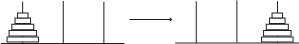
\includegraphics[width=0.85\linewidth]{images/Hanoi}
\caption{The Towers of Hanoi Puzzle\label{Hanoi}}
\end{figure}
\begin{activity}[]\label{HanoiProblem}
The ``Towers of Hanoi'' puzzle has three rods rising from a rectangular base with \(n\) rings of different sizes stacked in decreasing order of size on one rod. A legal move consists of moving a ring from one rod to another so that it does not land on top of a smaller ring. If \(m_n\) is the number of moves required to move all the rings from the initial rod to another rod that you choose, give a recurrence for \(m_n\). (Hint: suppose you already knew the number of moves needed to solve the puzzle with \(n-1\) rings.)%
\par\medskip\noindent%
\textbf{Solution.}\quad We can solve the puzzle in one step if there is one ring, so \(m_1=1\). If \(n>0\) and we want to move all the rings from the initial rod to rod 3, then first we solve the problem of moving all but the bottom ring to rod 2; this takes \(m_{n-1}\) steps, then we move the bottom ring to rod 3, then we solve the problem of moving all the remaining rings from rod 2 to rod 3. Thus we have \(m_n=2m_{n-1}+1\).%
\end{activity}
\begin{activity}[]\label{circlesinplane}
We draw \(n\) mutually intersecting circles in the plane so that each one crosses each other one exactly twice and no three intersect in the same point. (As examples, think of Venn diagrams with two or three mutually intersecting sets.) Find a recurrence for the number \(r_n\) of regions into which the plane is divided by \(n\) circles. (One circle divides the plane into two regions, the inside and the outside.) Find the number of regions with \(n\) circles. For what values of \(n\) can you draw a Venn diagram showing all the possible intersections of \(n\) sets using circles to represent each of the sets?%
\par\medskip\noindent%
\textbf{Solution.}\quad One circle defines two regions, the inside and outside. When we draw a second circle that intersects the first, we can start at one of the intersection points and go inside the first circle, cutting its region into two pieces, and then when we leave it we cut the outside region into two pieces. This suggests the general pattern. If we have drawn \(n-1\) circles and start a new one, each time we enter a circle, we start dividing a region into two pieces. Each time we leave a circle, we also start dividing a region into two pieces. Thus if we have \(r_n\) regions with \(n\) circles, to get the number of regions, we note that in going from \(n-1\) circles to \(n\) circles, we start with \(r_{n-1}\) regions, and divide \(2(n-1)\) of them in half, so we get \(2n-2\) new regions. This gives us \(r_n=r_{n-1}+2(n-1)\). Notice that by substitution of the formula \(r_{n-1}=r_{n-2} +2(n-2)\), we get \(r_n=r_{n-2}+ 2(n-2)
+2(n-1)\), and would guess that \(r_n=r_{n-3}+2(n-3)+2(n-2) +2(n-1)\). This leads to the conjecture%
\begin{equation*}
r_n=r_1  +2\cdot1+2\cdot2+\cdots+2\cdot(n-1)=r_1+2\sum_{i=1}^{n-1}
i=2+n(n-1).
\end{equation*}
%
\par
We can prove this formula by induction. When \(n=1\) we have \(2+1\cdot0\) regions. Assuming that \(n-1\) circles give us \(2+(n-1)(n-2)\) regions, for \(n\) circles we have \(2+(n-1)(n-2) +2(n-1)=2+n(n-1)\) regions. Thus the correctness of our formula for \(n-1\) circles implies its correctness when we have \(n\) circles, so for all positive integers \(n\), we get \(2+n(n-1)\) regions determined by \(n\) mutually intersecting circles. Two circles cannot touch more than twice, and if we let some of our \(n\) circles touch just once, or not at all, that would reduce the number of regions we would get. Similarly, allowing a circle to go through the intersection point of two other circles could only reduce the number of regions. So with \(n\) circles we could never have more than \(2+n(n-1)\) regions. In particular with 4 circles we get just 14 regions, rather than the 16 that would be required in a Venn diagram for four sets. We could prove, again by induction, that \(2+n(n-1)\lt 2^n\) for all \(n>3\), so it is not possible to draw a Venn diagram using circles to illustrate the intersections of four or more sets.%
\end{activity}
\typeout{************************************************}
\typeout{Subsection  Arithmetic Series (optional)}
\typeout{************************************************}
\subsection[{Arithmetic Series (optional)}]{Arithmetic Series (optional)}\label{subsection-18}
\begin{activity}[]\label{childsaving}
~\par
\begin{enumerate}[label=(\alph*)]
 \item A child puts away two dollars from her allowance each week. If she starts with twenty dollars, give a recurrence for the amount \(a_n\) of money she has after \(n\) weeks and find out how much money she has at the end of \(n\) weeks.%
\par\medskip\noindent%
\textbf{Solution.}\quad \(a_n=a_{n-1} +2\). Then by substitution \(a_n=a_{n-2}+2+2\), and so we conjecture that \(a_n = 20 +2n\). Since she adds two dollars to her savings each week for \(n\) weeks, she has adds 2n dollars to her original 20, which proves the formula. We could have used induction to prove it as well.%

~\par
\item A sequence that satisfies a recurrence of the form \(a_n=a_{n-1} +c\) is called an \emph{arithmetic progression}\index{arithmetic progression}\index{progression!arithmetic}. Find a formula in terms of the initial value \(a_0\) and the common difference \(c\) for the term \(a_n\) in an arithmetic progression and prove you are right.%
\par\medskip\noindent%
\textbf{Solution.}\quad \(a_n =a_o+cn\). The formula is valid with \(n=0\), and if \(a_{n-1}=a_0
+c(n-1)\), then \(a_n = a_0 +c(n-1) +c =a_0+cn\). Therefore the fact that \(a_{n-1}=a_0+ca_{n-1}\) implies the fact that \(a_n=a_0+cn\). Therefore by the principle of mathematical induction, \(a_n=a_0+cn\) for all nonnegative integers \(n\).%

~\par
\item A person who is earning \textdollar{}50,000 per year gets a raise of \textdollar{}3000 a year for \(n\) years in a row. Find a recurrence for the amount \(a_n\) of money the person earns over \(n+1\) years. What is the total amount of money that the person earns over a period of \(n+1\) years? (In \(n+1\) years, there are \(n\) raises.)%
\par\medskip\noindent%
\textbf{Solution.}\quad By {$\langle\langle$Unresolved xref, reference "arithmeticprogression"; check spelling or use "provisional" attribute$\rangle\rangle$} we saw that if \(b_n\) is the salary in year \(n\), then \(b_n=50,000 + 3000n\). If \(a_n\) is the total amount earned over the period of from year 0 through the end of year \(n\), a period of \(n+1\) years, then \(a_n=a_{n-1}+b_n=a_{n-1}+ 50,000+3000n\). Further, \(a_n=\sum_{i=0}^n b_i=\sum_{i=0}^n50,000 +3000i = 50,000(n+1)+3000\sum_{i=0}^n
i= 50,000(n+1) + 1500(n(n+1)\).%

~\par
\item An \emph{arithmetic series}\index{series!arithmetic}\index{arithmetic series} is a sequence \(s_n\) equal to the sum of the terms \(a_0\) through \(a_n\) of of an arithmetic progression. Find a recurrence for the sum \(s_n\) of an arithmetic progression with initial value \(a_0\) and common difference \(c\) (using the language of {$\langle\langle$Unresolved xref, reference "arithmeticprogression"; check spelling or use "provisional" attribute$\rangle\rangle$}). Find a formula for general term \(s_n\) of an arithmetic series.%
\par\medskip\noindent%
\textbf{Solution.}\quad \(s_n=\sum_{i=0}^n a_0 +ci =(n+1)a_0+c\sum_{i=0}^n i = (n+1)a_0
+cn(n+1)/2\).%

\end{enumerate}
\end{activity}
\typeout{************************************************}
\typeout{Subsection  First order linear recurrences}
\typeout{************************************************}
\subsection[{First order linear recurrences}]{First order linear recurrences}\label{subsection-19}
Recurrences such as those in \hyperref[subsetequation]{Equations~(\ref{subsetequation})} through \hyperref[secondorderlinear]{Equation~(\ref{secondorderlinear})} are called \emph{linear recurrences}, as are the recurrences of \hyperref[HanoiProblem]{Problems~\ref{HanoiProblem}} and \hyperref[circlesinplane]{Activity~\ref{circlesinplane}}. A \emph{linear recurrence}\index{recurrence!linear}\index{linear recurrence} is one in which \(a_n\) is expressed as a sum of functions of \(n\) times values of (some of the terms) \(a_i\) for \(i\lt n\) plus (perhaps) another function (called the \emph{driving function}\index{driving function}\index{function!driving}) of \(n\). A linear equation is called \emph{homogeneous}\index{homogeneous linear recurrence}\index{linear recurrence!homogeneous}\index{recurrence!linear homogeneous} if the driving function is zero (or, in other words, there is no driving function). It is called a \emph{constant coefficient linear recurrence}\index{linear recurrence!constant coefficient}\index{constant coefficient linear recurrence} if the functions that are multiplied by the \(a_i\) terms are all constants (but the driving function need not be constant).%
\begin{activity}[]\label{classifyrecurrences}
Classify the recurrences in \hyperref[subsetequation]{Equations~(\ref{subsetequation})} through \hyperref[secondorderlinear]{Equation~(\ref{secondorderlinear})} and \hyperref[HanoiProblem]{Problems~\ref{HanoiProblem}} and \hyperref[circlesinplane]{Activity~\ref{circlesinplane}} according to whether or not they are constant coefficient, and whether or not they are homogeneous.%
\par\medskip\noindent%
\textbf{Solution.}\quad \hyperref[subsetequation]{Recurrence~(\ref{subsetequation})} is first order, linear, constant coefficient, and homogeneous. \hyperref[bijectionequation]{Recurrence~(\ref{bijectionequation})} is first order, linear, and homogeneous, but not constant coefficient. \hyperref[arithmeticexample]{Recurrence~(\ref{arithmeticexample})} is first order, linear, constant coefficient but not homogeneous. \hyperref[geometricdriven]{Recurrence~(\ref{geometricdriven})} is first order, linear, constant coefficient but not homogeneous. \hyperref[secondorderlinear]{Recurrence~(\ref{secondorderlinear})} is not first order (it is second order), is linear, constant coefficient and homogeneous. The recurrence of \hyperref[HanoiProblem]{Problem~\ref{HanoiProblem}} is first order, linear, and constant coefficient, and that of \hyperref[circlesinplane]{Problem~\ref{circlesinplane}} is first order, linear, and constant coefficient.%
\end{activity}
\begin{activity}[]\label{firstordlinconst}
As you can see from \hyperref[classifyrecurrences]{Problem~\ref{classifyrecurrences}} some interesting sequences satisfy first order linear recurrences, including many that have constant coefficients, have constant driving term, or are homogeneous. Find a formula in terms of \(b\), \(d\), \(a_0\) and \(n\) for the general term \(a_n\) of a sequence that satisfies a constant coefficient first order linear recurrence \(a_n = ba_{n-1} + d\) and prove you are correct. If your formula involves a summation, try to replace the summation by a more compact expression.%
\par\medskip\noindent%
\textbf{Solution.}\quad Note that by the formula, \(a_{n-1}=ba_{n-2} +d\). Substituting this into the original equation for \(a_n\) gives \(a_n=b^2a_{n-2}+bd +d\). Repeating this kind of substitution gives us \(a_n=b^3a_{n-3} +b^2d +bd +d\). This suggests that \(a_n = a_0b^n +\sum_{i=0}^{n-1}db^i\). We would guess the same formula by writing out the first few values of \(a_i\), namely, \(a_0\), \(a_0b+d\), \(a_0b^2+db+d\), \(a_0b^3+b^2d+bd+d\), and so on. We prove our general formula by induction on \(n\). It is clearly true when \(n=0\) as there are no terms in the sum and \(b^0=1\). If we assume the formula is true when \(n=k-1\), we may write%
\begin{align*}
a_k \amp =\amp  ba_{k-1}+d\\
\amp =\amp b(a_0b^{k-1}+ b\left(\sum_{i=0}^{n-2}db^i\right) +d\\
\amp =\amp a_0b^n +\sum_{i=0}^{n-1}db^i
\end{align*}
%
\par
Thus the truth of our formula for \(n=k-1\) implies its truth for \(n=k\) and therefore by the principle of mathematical induction, it is true for all nonnegative integers \(n\).%
\par
We can give a more compact expression for the sum \(\sum_{i=0}^{n-1}db^i=d\sum_{i=0}^{n-1}b^i\). Recall from algebra that \((1+x)(1-x)= 1-x^2\), \((1+x+x^2)(1-x) = 1-x^3\), and in general \((1+x+x^2+\cdots
x^{n-1}))(1-x) = 1-x^n\). If you do not recall this formula, you can prove it by induction, or observe that%
\begin{align*}
\amp \amp (1+x+x^2+\cdots
x^{n-1}))(1-x)\\
\amp =\amp  (1+x+x^2+\cdots
x^{n-1})\cdot 1-(1+x+x^2+\cdots
x^{n-1})\cdot x\\
\amp =\amp  1+x+x^2+\cdots x^{n-1}-(x+x^2+\cdots+x^n)\rangle =\rangle  1-x^n.
\end{align*}
%
\par
Dividing the first and last terms by \(1-x\) gives us%
\begin{equation*}
\sum_{i=1}^{n-1}x^i={1-x^n\over 1-x}.
\end{equation*}
%
\par
Using this in our formula for \(a_n\) gives us \(a_n =a_ob^n+d{1-b^n\over 1-b}.\) This is valid except in the case \(b=1\) (in our computation with \(x\) above, we would be dividing by 0.) If \(b=1\) we get \(a_n =a_0 +nd\) for the sum.%
\end{activity}
\typeout{************************************************}
\typeout{Subsection  Geometric Series}
\typeout{************************************************}
\subsection[{Geometric Series}]{Geometric Series}\label{subsection-20}
A sequence that satisfies a recurrence of the form \(a_n=ba_{n-1}\) is called a \emph{geometric progression}\index{geometric progression}\index{progression!geometric}. Thus the sequence satisfying \hyperref[subsetequation]{Equation~(\ref{subsetequation})}, the recurrence for the number of subsets of an \(n\)-element set, is an example of a geometric progression. From your solution to \hyperref[firstordlinconst]{Problem~\ref{firstordlinconst}}, a geometric progression has the form \(a_n=a_0b^n\). In your solution to \hyperref[firstordlinconst]{Problem~\ref{firstordlinconst}} you may have had to deal with the sum of a geometric progression in just slightly different notation, namely \(\sum_{i=0}^{n-1}db^i\). A sum of this form is called a \emph{(finite) geometric series}.\index{geometric series}\index{series!geometric}%
\begin{activity}[]\label{sumgeometricseries}
Do this problem only if your final answer (so far) to \hyperref[firstordlinconst]{Problem~\ref{firstordlinconst}} contained the sum \(\sum_{i=0}^{n-1}db^i\).%
~\par
\begin{enumerate}[label=(\alph*)]
 \item Expand \((1-x)(1+x)\).  Expand \((1-x)(1+x+x^2)\). Expand \((1-x)(1+x+x^2+x^3)\).%
\par\medskip\noindent%
\textbf{Solution.}\quad \((1-x)(1+x)=1-x^2\). \((1-x)(1+x+x^2)=1-x^3\). \((1-x)(1+x+x^2+x^3)=1-x^4\).%

~\par
\item What do you expect \((1-b)\sum_{i=0}^{n-1} db^i\) to be?  What formula for \(\sum_{i=0}^{n-1}db^i\) does this give you?  Prove that you are correct.%
\par\medskip\noindent%
\textbf{Solution.}\quad We expect \((1-b)\sum_{i=0}^{n-1} db^i\) to be \(d(1-b^n)\). If \(b\not=1\), this gives us \(\sum_{i=0}^{n-1}db^i=d{1-b^n\over 1-b}.\) We can prove this by induction on \(n\). If \(n=0\) we get 0 for \(1-b^n\over 1-b\), and also for the sum \(\sum_{i=0}^{-1}db^i\), since that sum has no terms. Assuming the formula holds when \(n=k-1\), we may write%
\begin{align*}
\amp \amp \sum_{i=0}^{k-1} db^i\\
\amp =\amp \sum_{i=0}^{k-2}db^i+db^{k-1}\\
\amp =\amp d{1-b^{k-1}\over 1-b}+db^{k-1}\\
\amp =\amp { d-db^{k-1}  +db^{k-1}-db^k\over 1-b}\rangle =\rangle  d{1-b^k\over 1-b}.
\end{align*}
%
\par
Since the truth of the formula for \(n=k-1\) implies its truth for \(n=k\), by the principle of mathematical induction the formula is true for all nonnegative integers \(n\). If \(b=1\) we get the formula \(\sum_{i=0}^{n-1}db^i=dn\).%

\end{enumerate}
\end{activity}
In \hyperref[firstordlinconst]{Problem~\ref{firstordlinconst}} and \hyperref[sumgeometricseries]{perhaps~\ref{sumgeometricseries}} you proved an important theorem.%
\begin{theorem}[{}]\label{theorem-2}
If \(b\not=1\) and \(a_n=ba_{n-1} +d\), then \(\displaystyle a_n =
a_0b^n + d{1-b^n\over 1-b}\). If \(b=1\), then, \(\displaystyle a_n =
a_0 +nd\)%
\end{theorem}
\begin{corollary}[{}]\label{corollary-1}
If \(b\not=1\), then \(\displaystyle \sum_{i=0}^{n-1}b^i =
{1-b^n\over 1-b}\). If \(b=1\), \(\displaystyle \sum_{i=0}^{n-1}b^i =n\).%
\end{corollary}
\typeout{************************************************}
\typeout{Section 1.3 Graphs and Trees}
\typeout{************************************************}
\section[{Graphs and Trees}]{Graphs and Trees}\label{sec_induction-graphstrees}
\typeout{************************************************}
\typeout{Subsection  Undirected graphs}
\typeout{************************************************}
\subsection[{Undirected graphs}]{Undirected graphs}\label{graphsection}
In \hyperref[Ramseysection]{Section~} we introduced the idea of a directed graph. Graphs consist of vertices and edges. We describe vertices and edges in much the same way as we describe points and lines in geometry: we don't really say what vertices and edges are, but we say what they do. We just don't have a complicated axiom system the way we do in geometry. A \emph{graph}\index{graph} consists of a set \(V\) called a vertex set and a set \(E\) called an edge set. Each member of \(V\) is called a \emph{vertex}\index{vertex} and each member of \(E\) is called an \emph{edge}.\index{edge} Associated with each edge are two (not necessarily different) vertices called its endpoints. We draw pictures of graphs by drawing points to represent the vertices and line segments (curved if we choose) whose endpoints are at vertices to represent the edges. In \hyperref[Threegraphs]{Figure~\ref{Threegraphs}} we show three pictures of graphs.%
\begin{figure}
\centering
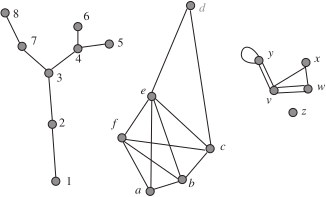
\includegraphics[width=0.95\linewidth]{images/threegraphs}
\caption{Three different graphs\label{Threegraphs}}
\end{figure}
Each grey circle in the figure represents a vertex; each line segment represents an edge. You will note that we labelled the vertices; these labels are names we chose to give the vertices. We can choose names or not as we please. The third graph also shows that it is possible to have an edge that connects a vertex (like the one labelled \(y\)) to itself or it is possible to have two or more edges (like those between vertices \(v\) and \(y\)) between two vertices. The \emph{degree}\index{vertex!degree of}\index{degree of a vertex} of a vertex is the number of times it appears as the endpoint of edges; thus the degree of \(y\) in the third graph in the figure is four.%
\begin{activity}[]\label{activity-92}
In the graph on the left in \hyperref[Threegraphs]{Figure~\ref{Threegraphs}}, what is the degree of each vertex?%
\par\medskip\noindent%
\textbf{Solution.}\quad The degree of vertex 1 is one, of vertex 2 is two, of vertex 3 is three, of vertex 4 is three, of vertex 5 is one, of vertex 6 is one, of vertex 7 is two, of vertex 8 is one.%
\end{activity}
\begin{activity}[]\label{activity-93}
For each graph in \hyperref[Threegraphs]{Figure~\ref{Threegraphs}} is the number of vertices of odd degree even or odd?%
\par\medskip\noindent%
\textbf{Solution.}\quad In all three cases it is even.%
\end{activity}
\begin{activity}[]\label{activity-94}
The sum of the degrees of the vertices of a (finite) graph is related in a natural way to the number of edges.%
~\par
\begin{enumerate}[label=(\alph*)]
 \item What is the relationship?%
\par\medskip\noindent%
\textbf{Solution.}\quad The sum of the degrees of the vertices is twice the number of edges.%

~\par
\item Find a proof that what you say is correct that uses induction on the number of edges.  Hint:  To make your inductive step, think about what happens to a graph if you delete an edge.%
\par\medskip\noindent%
\textbf{Solution.}\quad If a graph has no edges, then the sum of the degrees of the vertices is 0, which is twice the number of edges. Now suppose that whenever a graph has \(n-1\) edges, the sum of the degrees of the vertices is twice the number of edges. Let \(G\) be a graph with \(n\) edges, and delete an edge from \(G\) to get \(G'\). The the sum of the degrees of \(G'\) is \(2(n-1)\), and adding the edge back into \(G'\) to get \(G\) either increases the degrees of exactly two vertices by one each or increases the degree of one vertex by 2. Thus the sum of the degrees of the vertices of \(G\) is \(2n\), which is twice the number of edges. Thus by the principle of mathematical induction, for all nonnegative integers \(n\), if a graph has \(n\) edges, then the sum of the degrees of the vertices is twice the number of edges.%

~\par
\item Find a proof that what you say is correct that uses induction on the number of vertices.%
\par\medskip\noindent%
\textbf{Solution.}\quad If a graph has no vertices, then the sum of the degrees of the vertices is 0, which is twice the number of edges. Now suppose that whenever a graph has \(n-1\) vertices, the sum of the degrees is twice the number of edges. Let \(G\) be a graph with \(n\) vertices. Delete one vertex \(x\) and all edges it is incident with. By our inductive hypothesis the sum of the degrees of the vertices of the resulting graph is twice the number of edges. Now replace the vertex \(x\) and add in the edges connecting it to other vertices in the graph. Each time you add in an edge, you increase the degree of \(x\) by one and of one other vertex by one. Finally add in any edges connecting \(x\) to itself. Each of these increases the degree of \(x\) by two. Thus for each edge we added, the sum of the degrees of the vertices increased by two, so the sum of the degrees of the vertices of \(G\) is still twice the number of edges. Therefore by the principle of mathematical induction, for all nonnegative integers \(n\), if a graph has \(n\) vertices, then the sum of the degrees of its vertices is even.%

~\par
\item Find a proof that what you say is correct that does not use induction.%
\par\medskip\noindent%
\textbf{Solution.}\quad The sum of the degrees of the vertices is the sum over all edges of the number of times that edge touches a vertex, which is twice the number of edges.%

\end{enumerate}
\end{activity}
\begin{activity}[]\label{activity-95}
What can you say about the number of vertices of odd degree in a graph?%
\par\medskip\noindent%
\textbf{Solution.}\quad The number of vertices of odd degree must be even, because otherwise the sum of the degrees of the vertices would be odd.%
\end{activity}
\typeout{************************************************}
\typeout{Subsection  Walks and paths in graphs}
\typeout{************************************************}
\subsection[{Walks and paths in graphs}]{Walks and paths in graphs}\label{subsection-22}
A \terminology{walk}\index{walk} in a graph is an alternating sequence \(v_0e_1v_1\ldots
e_iv_i\) of vertices and edges such that edge \(e_i\) connects vertices \(v_{i-1}\) and \(v_i\). A graph is called connected if, for any pair of vertices, there is a walk starting at one and ending at the other.%
\begin{activity}[]\label{connectedanddisconnected}
Which of the graphs in \hyperref[Threegraphs]{Figure~\ref{Threegraphs}} is connected?%
\par\medskip\noindent%
\textbf{Solution.}\quad They first two connected; the third is not.%
\end{activity}
\begin{activity}[]\label{activity-97}
A \terminology{path}\index{path!in graph} in a graph is a walk with no repeated vertices.  Find the longest path you can in the third graph of \hyperref[Threegraphs]{Figure~\ref{Threegraphs}}.%
\par\medskip\noindent%
\textbf{Solution.}\quad The path from \(y\) to \(v\) to \(x\) to \(w\) is a typical longest path. There are quite a few others. Notice you have two choices for the edge to use to get from \(y\) to \(v\).%
\end{activity}
\begin{activity}[]\label{activity-98}
A \terminology{cycle}\index{cycle!in graph} in a graph is a walk whose first and last vertex are equal but which has no other repeated vertices.  Which graphs in \hyperref[Threegraphs]{Figure~\ref{Threegraphs}} have cycles?  What is the largest number of edges in a cycle in the second graph in \hyperref[Threegraphs]{Figure~\ref{Threegraphs}}?  What is the smallest number of edges in a cycle in the third graph in \hyperref[Threegraphs]{Figure~\ref{Threegraphs}}?%
\par\medskip\noindent%
\textbf{Solution.}\quad The second and third graphs have cycles. The largest number of edges in a cycle in the second graph is six; the smallest number of edges in a cycle in the third graph is one.%
\end{activity}
\begin{activity}[]\label{activity-99}
A connected graph with no cycles is called a \terminology{tree}\index{tree}.  Which graphs, if any, in \hyperref[Threegraphs]{Figure~\ref{Threegraphs}} are trees?%
\par\medskip\noindent%
\textbf{Solution.}\quad The first graph is a tree.%
\end{activity}
\typeout{************************************************}
\typeout{Subsection  Counting vertices, edges, and paths in trees}
\typeout{************************************************}
\subsection[{Counting vertices, edges, and paths in trees}]{Counting vertices, edges, and paths in trees}\label{subsection-23}
\begin{activity}[]\label{Noverticesandedgesoftree}
Draw some trees and on the basis of your examples, make a conjecture about the relationship between the number of vertices and edges in a tree. Prove your conjecture. (Hint: what happens if you choose an edge and delete it, but not its endpoints?)%
\par\medskip\noindent%
\textbf{Solution.}\quad The number of edges of a tree is one less than the number of vertices. We prove this by strong induction on the number of edges. First, if a tree has no edges, it can have only one vertex (otherwise it is not connected). Thus the number of edges is one less than the number of vertices. Now suppose that if a tree has fewer than \(n\) edges, it the number of edges is one less than the number of vertices. Choose an edge \(e\) with endpoints \(x\) and \(y\) in the tree and remove it. The resulting graph is not connected, for if it were, the path remaining between the endpoints of \(e\), together with \(e\), would form a cycle. Every vertex in the tree is connected to \(x\) by a path; those connected by a path not using \(e\) still remain connected to \(x\). Similarly those connected to \(y\) by a path in the tree that does not use the edge \(e\) remain connected to \(y\) after \(e\) is deleted. Every vertex is connected to \(x\) by a path in the tree and every vertex is connected to \(y\) by a path in the tree. If a vertex \(v\) were connected to \(x\) by a path using the edge \(e\) and to \(y\) by a path using the edge \(e\), that would mean that we have a path from \(v\) to \(x\) and then through \(e\) to \(y\) and also a path from \(v\) to \(y\) and then through \(e\) to \(x\). Thus taking \(e\) out of these two paths would give us a path from \(v\) to \(x\) and a path from \(v\) to \(y\), neither of which used \(e\). Thus when we removed the edge \(e\), there would still be a path from \(x\) to \(y\), and adding \(e\) to this path would give a cycle. Therefore each vertex is connected to either \(x\) or \(y\), but not both, by a path that does not use \(e\). Therefore when we remove \(e\), the graph that remains consists of two trees, the tree of all vertices connected to \(x\) and the tree of all vertices connected to \(y\). Each of these trees has fewer edges than the original tree, so if they have \(m_1\) and \(m_2\) vertices respectively, they have, by the inductive hypothesis, \(m_1-1\) and \(m_2-1\) edges respectively. But together they have all the vertices of the original tree, so the original tree has \(m_1+m_2\) vertices, and has \(m_1-1+m_2-1 +1=m)_1+m_2-1\) edges, the edges of each of the two smaller trees as well as the edge \(e\). Therefore the number of edges of the original tree is one less than the number of vertices. Therefore by the strong principle of mathematical induction, the number of edges of a tree is one less than the number of vertices.%
\end{activity}
\begin{activity}[]\label{activity-101}
What is the minimum number of vertices of degree one in a finite tree? What is it if the number of vertices is bigger than one? Prove that you are correct.%
\par\medskip\noindent%
\textbf{Solution.}\quad The minimum is zero, which happens with a tree with one vertex. If the tree has more than one vertex, the minimum number of vertices of degree one is two. To prove this, we prove that every tree with two or more vertices has at least two vertices of degree two. Note that a tree with two vertices has exactly two vertices of degree 2. Now take a tree with more than two vertices. Remove an edge \(e\) without removing its endpoints. As in the solution to \hyperref[Noverticesandedgesoftree]{Problem~\ref{Noverticesandedgesoftree}} this gives two trees. We may assume inductively that each has at least two vertices of degree 1, or else is a single vertex. When we put \(e\) back in, it connects one vertex in one tree to one in the other. If both these vertices have degree 1 in their trees, there will be at least one vertex of degree 1 remaining in each tree, so there will be at least two vertices of degree 1 in the tree we get. If exactly one of these vertices is a tree with one vertex after the removal of \(e\), when we connect it to the other tree, we will remove at most one increase the degree of at most one vertex of degree 1 and will create a new vertex of degree 1, so the tree that results still has at least two vertices of degree 1. Therefore by the strong principle of mathematical induction, every tree with more than two vertices has at least two vertices of degree 1. Since a two-vertex tree has two vertices of degree 1, the minimum number of vertices of degree 1 in a tree with two or more vertices is two. (In fact a path with \(n\) vertices is a tree and it has exactly two vertices of degree one also.)%
\end{activity}
\begin{activity}[]\label{activity-102}
In a tree, given two vertices, how many paths can you find between them? Prove that you are correct.%
\par\medskip\noindent%
\textbf{Solution.}\quad Exactly one. Suppose there were two distinct paths \(P_1\) and \(P_2\) from \(x\) to \(y\). As they leave \(x\), they might leave on the same edge or on different edges. However, since they are different, there must be some first vertex \(x'\) on both paths so that when leave \(x'\) (as we go from \(x\) to \(y\)), they leave on different edges. Then since they must both enter \(y\), there must be some first vertex \(y'\), following \(x'\) on both paths as we go from \(x\) to \(y\), such that the two paths enter \(y'\) on two different edges. Then the portion of path 1 from \(x'\) to \(y'\) followed by the portion of path 2 from \(y'\) to \(x'\) will be a cycle. This is impossible in a tree, so the supposition that there were two distinct paths is impossible.%
\end{activity}
\begin{activity}[]\label{Prufer}
How many trees are there on the vertex set \(\{1,2\}\)? On the vertex set \(\{1,2,3\}\)? When we label the vertices of our tree, we consider the tree which has edges between vertices 1 and 2 and between vertices 2 and 3 different from the tree that has edges between vertices 1 and 3 and between 2 and 3. See \hyperref[differenttrees]{Figure~\ref{differenttrees}}.%
\begin{figure}
\centering
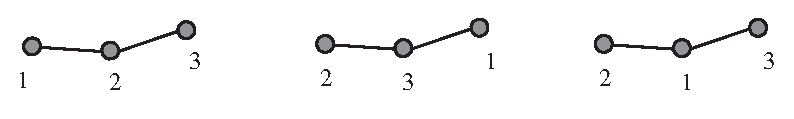
\includegraphics[width=0.8\linewidth]{images/threetrees}
\caption{The three labelled trees on three vertices\label{differenttrees}}
\end{figure}
How many (labelled) trees are there on four vertices? You don't have a lot of data to guess from, but try to guess a formula for the number of labelled trees with vertex set \(\{1,2,\cdots,n\}\). (If you organize carefully, you can figure out how many labelled trees there are with vertex set \(\{1,2,3,4,5\}\) to help you make your conjecture.) Given a tree with two or more vertices, labelled with positive integers, we define a sequence \(b_1,b_2,\ldots\) of integers inductively as follows: If the tree has two vertices, the sequence consists of one entry, namely the label of the vertex with the larger label. Otherwise, let \(a_1\) be the lowest numbered vertex of degree 1 in the tree. Let \(b_1\) be the label of the unique vertex in the tree adjacent to \(a_1\) and write down \(b_1\). Given \(a_{i-1}\) and \(b_{i-1}\), let \(a_i\) be the lowest numbered vertex of degree 1 in the tree you get by deleting \(a_1\) through \(a_{i-1}\) and let \(b_i\) be the unique vertex in this new tree adjacent to \(a_i\). We use \(b\) to stand for the sequence of \(b_i\)s we get in this way. For example in the tree (the first graph) in \hyperref[Threegraphs]{Figure~\ref{Threegraphs}}, \(a_1\) is 1 and the sequence \(b\) is 234478. (If you are unfamiliar with inductive (recursive) definition, you might want to write down some other labelled trees on eight vertices and construct the sequence of \(b_i\)s.) How long will the sequence \(b\) be if it is applied to a tree with \(n\) vertices (labelled with 1 through \(n\))? What can you say about the last member of the sequence of \(b_i\)s? Can you tell from the sequence of \(b_i\)s what \(a_1\) is? Find a bijection between labelled trees and something you can ``count'' that will tell you how many labelled trees there are on \(n\) labelled vertices.%
\par\medskip\noindent%
\textbf{Solution.}\quad There is one labelled tree on two vertices. We know there are three labelled trees on three vertices, and they all are paths. The difference among them is which vertex is the central vertex on the path. On four vertices a tree either has a vertex of degree 3 (there are four such trees) or it is a path, in which case there are six choices for the two vertices of degree 2, and for each choice of these two vertices, there are two different ways to attach the remaining vertices to them as vertices of degree 1. Thus there are \(12+4=16\) trees on four vertices. Assuming this is not enough data for a good guess, note that on five vertices, we either have a vertex of degree 4 (there are five such trees), or we have a vertex of degree three which must be adjacent to a vertex of degree two in order to have five vertices. There are \(5\cdot4=20\) ways to choose these two vertices; then three more choices we can make for the degree one vertex attached to the degree 2 vertex. Thus we have 60 trees with a vertex of degree three. If we have neither a vertex of degree four nor a vertex of degree three, then the tree is a path. We have \(\binom{5}{2}=10\) ways to choose the two vertices of degree one, and then there are \(3!=6\) ways to arrange the remaining vertices along the path, so we have 60 paths. Thus we have \(125\) trees on five vertices. These computations suggest there are \(n^{n-2}\) labelled trees on \(n\) vertices, which is what we shall prove with the sequences of \(a\)\/s and \(b\)\/s.%
\par
On a tree with \(n\) vertices, the sequence \(b\) will have length \(n-1\). The last member of the sequence \(b\) will be \(n\). Vertex \(n\) can not be in the sequence \(a\), because the tree that remains after we delete an \(a_i\) will have at least two vertices of degree 1, so the one of smaller degree will be \(a_{i+1}\). Thus we never delete the vertex \(n\) from the tree. Therefore when we choose the last \(b\), we have vertex \(n\) and one other vertex, so the other vertex is our \(a\)-vertex and \(n\) is the vertex adjacent to it. \(a_1\) will be the smallest number that is not in the sequence of \(b\)'s. This tells us one edge of the tree, namely the edge between \(a_1\) and \(b_1\). The vertex \(a_2\) will be the smallest number different from \(a_1\) not in the sequence \(b_2\) through \(b_{n-1}\). In general, \(a_i\) will be the smallest vertex different from \(a_1\) through \(a_{i-1}\) not in the sequence \(b_i\) through \(b_{n-1}\), which gives us all \(n-1\) edges of the tree (edge \(i\) goes from \(a_i\) to \(b_i\)). Thus there is a bijection between trees and the sequences \(b_1\) through \(b_{n-1}\). But since \(b_{n-1}=n\), there is also a bijection between trees and the sequences \(b_1\) through \(b_{n-2}\). But given a sequence of numbers \(c_1,c_2,\ldots,c_{n-2},c_{n-1}\), all between 1 and \(n\) and with \(c_{n-1}=n\), there is always a smallest number \(a_1\) not in the sequence, and given \(a_1,
a_2, \ldots a_{i-1}\), there is always a smallest number not in the sequence \(c_i\) through \(c_{n-1}\) and different from the \(a_i\)s already chosen, so we can construct the edges from \(a_i\) to \(c_i\). Further, if we start with the edge from \(a_{n-1}\) to \(c_{n-1}\) and work backwards, we will always have a connected graph and will always be adding a vertex of degree 1 to it, so we will have no cycles. Therefore we will get a tree. Thus we have a bijection between labelled trees on \(n\) vertices and sequences of length \(n-2\) consisting of members of \([n]\). There are \(n^{n-2}\) such sequences, and thus \(n^{n-2}\) labelled trees on \(n\) vertices.%
\end{activity}
The sequence \(b_1,b_2,\ldots, b_{n-2}\) in \hyperref[Prufer]{Problem~\ref{Prufer}} is called a \emph{Prüfer coding} or \emph{Prüfer code} for the tree. There is a good bit of interesting information encoded into the Prüfer code for a tree.%
\begin{activity}[]\label{activity-104}
What can you say about the Prüfer code for a tree with exactly two vertices of degree 1? Does this characterize such trees?%
\par\medskip\noindent%
\textbf{Solution.}\quad It consists of \(n-2\) distinct numbers between 1 and \(n\). Any such Prüfer code is the code of a tree with exactly two vertices of degree one.%
\end{activity}
\begin{activity}[]\label{activity-105}
What can you determine about the degree of the vertex labelled \(i\) from the Prufer code of the tree?%
\par\medskip\noindent%
\textbf{Solution.}\quad The degree of a vertex in a tree is one more than the number of times the vertex appears in the Prüfer code of the tree.%
\end{activity}
\begin{activity}[]\label{activity-106}
What is the number of (labelled) trees on \(n\) vertices with three vertices of degree 1? (Assume they are labelled with the integers 1 through \(n\).)%
\par\medskip\noindent%
\textbf{Solution.}\quad There are \(\binom{n}{3}\) ways to choose the three vertices of degree one. Each of the other \(n-3\) vertices must appear in the Prüfer Code, so one must appear twice. We have \(n-3\) ways to choose that one vertex and \(\binom{n-2}{2}\binom{n-4}{1}\binom{n-5}{1}\cdots\binom{1}{1} ={(n-2)!\over 2!}\) ways to choose which of the \(n-2\) places to use for which vertices in the Prüfer code. Thus there are \(\binom{n}{3}(n-3){(n-2)!\over 2}= {n!(n-2)(n-3)\over 12}\) labelled trees with three vertices of degree one.%
\end{activity}
\typeout{************************************************}
\typeout{Subsection  Spanning trees}
\typeout{************************************************}
\subsection[{Spanning trees}]{Spanning trees}\label{subsection-24}
Many of the applications of trees arise from trying to find an efficient way to connect all the vertices of a graph. For example, in a telephone network, at any given time we have a certain number of wires (or microwave channels, or cellular channels) available for use. These wires or channels go from a specific place to a specific place. Thus the wires or channels may be thought of as edges of a graph and the places the wires connect may be thought of as vertices of that graph. A tree whose edges are some of the edges of a graph \(G\) and whose vertices are all of the vertices of the graph \(G\) is called a \emph{spanning tree}\index{spanning tree}\index{tree!spanning} of \(G\). A spanning tree for a telephone network will give us a way to route calls between any two vertices in the network. In \hyperref[spanningtrees]{Figure~\ref{spanningtrees}} we show a graph and all its spanning trees.%
\begin{figure}
\centering
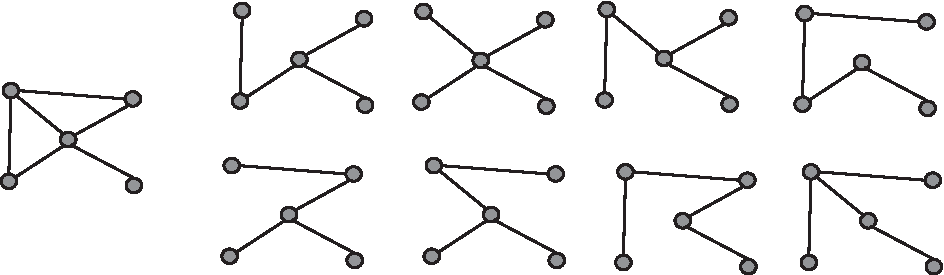
\includegraphics[width=0.95\linewidth]{images/spanningtrees}
\caption{A graph and all its spanning trees.\label{spanningtrees}}
\end{figure}
\begin{activity}[]\label{activity-107}
Show that every connected graph has a spanning tree. It is possible to find a proof that starts with the graph and works ``down'' towards the spanning tree and to find a proof that starts with just the vertices and works ``up'' towards the spanning tree. Can you find both kinds of proof?%
\par\medskip\noindent%
\textbf{Solution.}\quad Here are three proofs:%
\par
Start with a connected graph, and if you can find a cycle, remove one edge of that cycle. Repeat this process until you get a tree. You will get a tree, because removing an edge of a cycle reduces the number of cycles but leaves the graph connected. This tree will be a spanning tree of the original graph.%
\par
Start with the original vertex set and no edges for a graph \(H\). Go through the edges of the original graph \(G\) one at a time, and if you can add an edge of \(G\) to the graph \(H\) without creating a cycle, do so. Otherwise discard the edge and go on to the next one. This will give you a graph \(H\) with no cycles, and if it were not connected, there would be an edge in \(G\) between two vertices not yet connected in \(H\). (If there weren't, the graph you just constructed would be connected.) Thus you get a spanning tree.%
\par
Start with vertex 1 and no edges as a graph \(H\). Take an edge from it to another vertex. Add that edge and vertex to \(H\). Now take an edge from one of the vertices you currently have to yet another vertex of the original graph. Add that vertex and edge to \(H\). Repeat this process until you can find no such edge. You will get a tree because each edge you add connects a vertex of degree 1 to a tree you have already constructed. Since the original graph is connected, there must always be an edge from the current set of vertices you are considering to something not in that set.%
\end{activity}
\typeout{************************************************}
\typeout{Subsection  Minimum cost spanning trees}
\typeout{************************************************}
\subsection[{Minimum cost spanning trees}]{Minimum cost spanning trees}\label{subsection-25}
Our motivation for talking about spanning trees was the idea of finding a minimum number of edges we need to connect all the edges of a communication network together. In many cases edges of a communication network come with costs associated with them. For example, one cell-phone operator charges another one when a customer of the first uses an antenna of the other. Suppose a company has offices in a number of cities and wants to put together a communication network connecting its various locations with high-speed computer communications, but to do so at minimum cost. Then it wants to take a graph whose vertices are the cities in which it has offices and whose edges represent possible communications lines between the cities. Of course there will not necessarily be lines between each pair of cities, and the company will not want to pay for a line connecting city \(i\) and city \(j\) if it can already connect them indirectly by using other lines it has chosen. Thus it will want to choose a spanning tree of minimum cost among all spanning trees of the communications graph. For reasons of this application, if we have a graph with numbers assigned to its edges, the sum of the numbers on the edges of a spanning tree of \(G\) will be called the \emph{cost}\index{spanning tree!cost of}\index{tree!spanning!cost of}\index{cost of a spanning tree} of the spanning tree.%
\begin{activity}[]\label{mincostspantree}
Describe a method (or better, two methods different in at least one aspect) for finding a spanning tree of minimum cost in a graph whose edges are labelled with costs, the cost on an edge being the cost for including that edge in a spanning tree. Prove that your method(s) work.\index{minimum cost spanning tree}\index{spanning tree!minimum cost}\index{tree!spanning!minimum cost}%
\par\medskip\noindent%
\textbf{Solution.}\quad Start with vertex, number it vertex 1, and choose the least costly edge leaving it. Number the new vertex 2. Given your current set of vertices and edges, choose the least costly edge leaving that set, and if your set has \(i-1\) vertices, label the new vertex \(i\). You will always have a tree as you go along since you are adding a vertex of degree 1 to a tree you already have. You will get a spanning tree because the graph you start with is connected. If your tree did not have the lowest cost among all spanning trees, there would be some smallest \(i\) such that there is an edge from vertex \(i\) in a least cost spanning tree that is not in your tree. Since we chose the least \(i\), the edge we just chose from vertex \(i\) goes to a higher-numbered vertex. Thus you could have chosen that edge as you were constructing your tree, so there cannot be a tree of lower total cost than the one you chose.%
\par
Alternatively, start with the vertex set of the graph and no edges. Choose an edge of least cost. Repeat the following until it cannot be repeated. Given the set of edges you have so far, choose an edge of least cost among all edges that do not form a cycle with edges you already have. The graph you get will have no cycles, and it will have to be connected, because otherwise there would be an edge in the original graph that connects two vertices in the graph you just constructed. Thus you will have a tree. Suppose there is another tree with lower total cost. Choose such a tree with as many edges as common with your tree as possible. Then there is some edge \(e\) of this tree of lowest cost among all edges connecting two vertices that are not connected by an edge in your tree. Suppose the cost of this edge is \(c\). Since these vertices are connected by some path in your tree, when you were considering edges of cost \(c\), these two vertices were already connected by a path in your tree. There must be some edge \(f\) on that path not in the least cost tree. The edge \(f\) was already in your tree while you were considering edges of cost \(c\), so its cost is no more than \(c\). Adding \(f\) to the tree of least cost gives a cycle. All edges on that cycle that are not in your tree have cost at least \(c\) by our choice of \(e\). But since \(f\) was from your tree, there must be some edge \(g\) of the cycle that is in the least cost tree that but not in your tree. Removing \(g\) from the least cost tree and adding \(f\) cannot increase the cost of the tree, but it gives a tree that has one more edge in common with your tree. This contradicts the choice of the least cost tree, so there must have been no tree of lower total cost than the one you constructed.%
\end{activity}
The method you used in \hyperref[mincostspantree]{Problem~\ref{mincostspantree}} is called a \emph{greedy method}\index{greedy method}, because each time you made a choice of an edge, you chose the least costly edge available to you.%
\typeout{************************************************}
\typeout{Subsection  The deletion/contraction recurrence for spanning trees}
\typeout{************************************************}
\subsection[{The deletion/contraction recurrence for spanning trees}]{The deletion/contraction recurrence for spanning trees}\label{subsection-26}
There are two operations on graphs that we can apply to get a recurrence (though a more general kind than those we have studied for sequences) which will let us compute the number of spanning trees of a graph. The operations each apply to an edge \(e\) of a graph \(G\). The first is called \emph{deletion};\index{deletion} we \emph{delete} the edge \(e\) from the graph by removing it from the edge set. \hyperref[twodeletions]{Figure~\ref{twodeletions}} shows how we can delete edges from a graph to get a spanning tree.%
\begin{figure}
\centering
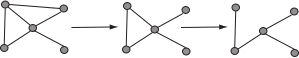
\includegraphics[width=0.6\linewidth]{images/twodeletions}
\caption{Deleting two appropriate edges from this graph gives a spanning tree.\label{twodeletions}}
\end{figure}
The second operation is called \emph{contraction}.%
\begin{figure}
\centering
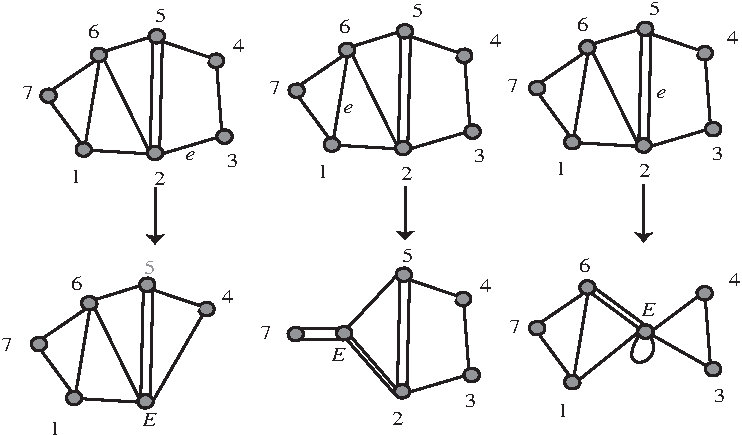
\includegraphics[width=0.65\linewidth]{images/threecontractions}
\caption{The results of contracting three different edges in a graph.\label{threecontractions}}
\end{figure}
Contractions of three different edges in the same graph are shown in \hyperref[threecontractions]{Figure~\ref{threecontractions}}. Intuitively, we contract an edge by shrinking it in length until its endpoints coincide; we let the rest of the graph ``go along for the ride.'' To be more precise, we \emph{contract}\index{contraction} the edge \(e\) with endpoints \(v\) and \(w\) as follows: \leavevmode%
\begin{enumerate}
\item\hypertarget{li-30}{}remove all edges having either \(v\) or \(w\) or both as an endpoint from the edge set,%
\item\hypertarget{li-31}{}remove \(v\) and \(w\) from the vertex set,%
\item\hypertarget{li-32}{}add a new vertex \(E\) to the vertex set,%
\item\hypertarget{li-33}{}add an edge from \(E\) to each remaining vertex that used to be an endpoint of an edge whose other endpoint was \(v\) or \(w\), and add an edge from \(E\) to \(E\) for any edge other than \(e\) whose endpoints were in the set \(\{v,w\}\).%
\end{enumerate}
%
\par
We use \(G-e\) (read as \(G\) minus \(e\)) to stand for the result of deleting \(e\) from \(G\), and we use \(G/e\) (read as \(G\) contract \(e\)) to stand for the result of contracting \(e\) from \(G\).%
\begin{activity}[]\label{activity-109}
How do the number of spanning trees of \(G\) not containing the edge \(e\) and the number of spanning trees of \(G\) containing \(e\) relate to the number of spanning trees of \(G-e\) and \(G/e\)? Use \(\#(G)\) to stand for the number of spanning trees of \(G\) (so that, for example, \(\#(G/e)\) stands for the number of spanning trees of \(G/e\)). Find an expression for \(\#(G)\) in terms of \(\#(G/e)\) and \(\#(G-e)\). This expression is called the \emph{deletion-contraction recurrence}\index{deletion-contraction recurrence}\index{recurrence!deletion-contraction}. Use it to compute the number of spanning trees of the graph in \hyperref[spantreeexercise]{Figure~\ref{spantreeexercise}}.%
\begin{figure}
\centering
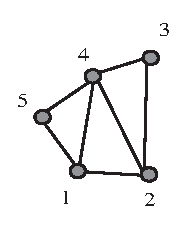
\includegraphics[width=0.2\linewidth]{images/spantreeexercise}
\caption{A graph.\label{spantreeexercise}}
\end{figure}
\par\medskip\noindent%
\textbf{Solution.}\quad The number of spanning trees of \(G\) not containing \(e\) is the number of spanning trees of \(G-e\). The number of spanning trees of \(G\) containing the edge \(e\) is the number of spanning trees of \(G/e\). Therefore \(\#(G) =\#(G-e)
+\#(G/e)\). Applying the formula twice to \(G\) gives%
\begin{align*}
\#(G)
\amp =\amp \#(G-\{1,2\}-\{2,3\}) + \#((G-\{1,2\})/\{2,3\})\\
\amp +\amp
\#((G/\{1,2\})-\{2,3\}) +
\#(G/\{1,2\}/\{2,3\}).
\end{align*}
%
\par
We now show the four graphs on the right hand side of the equation.%
\begin{figure}
\centering
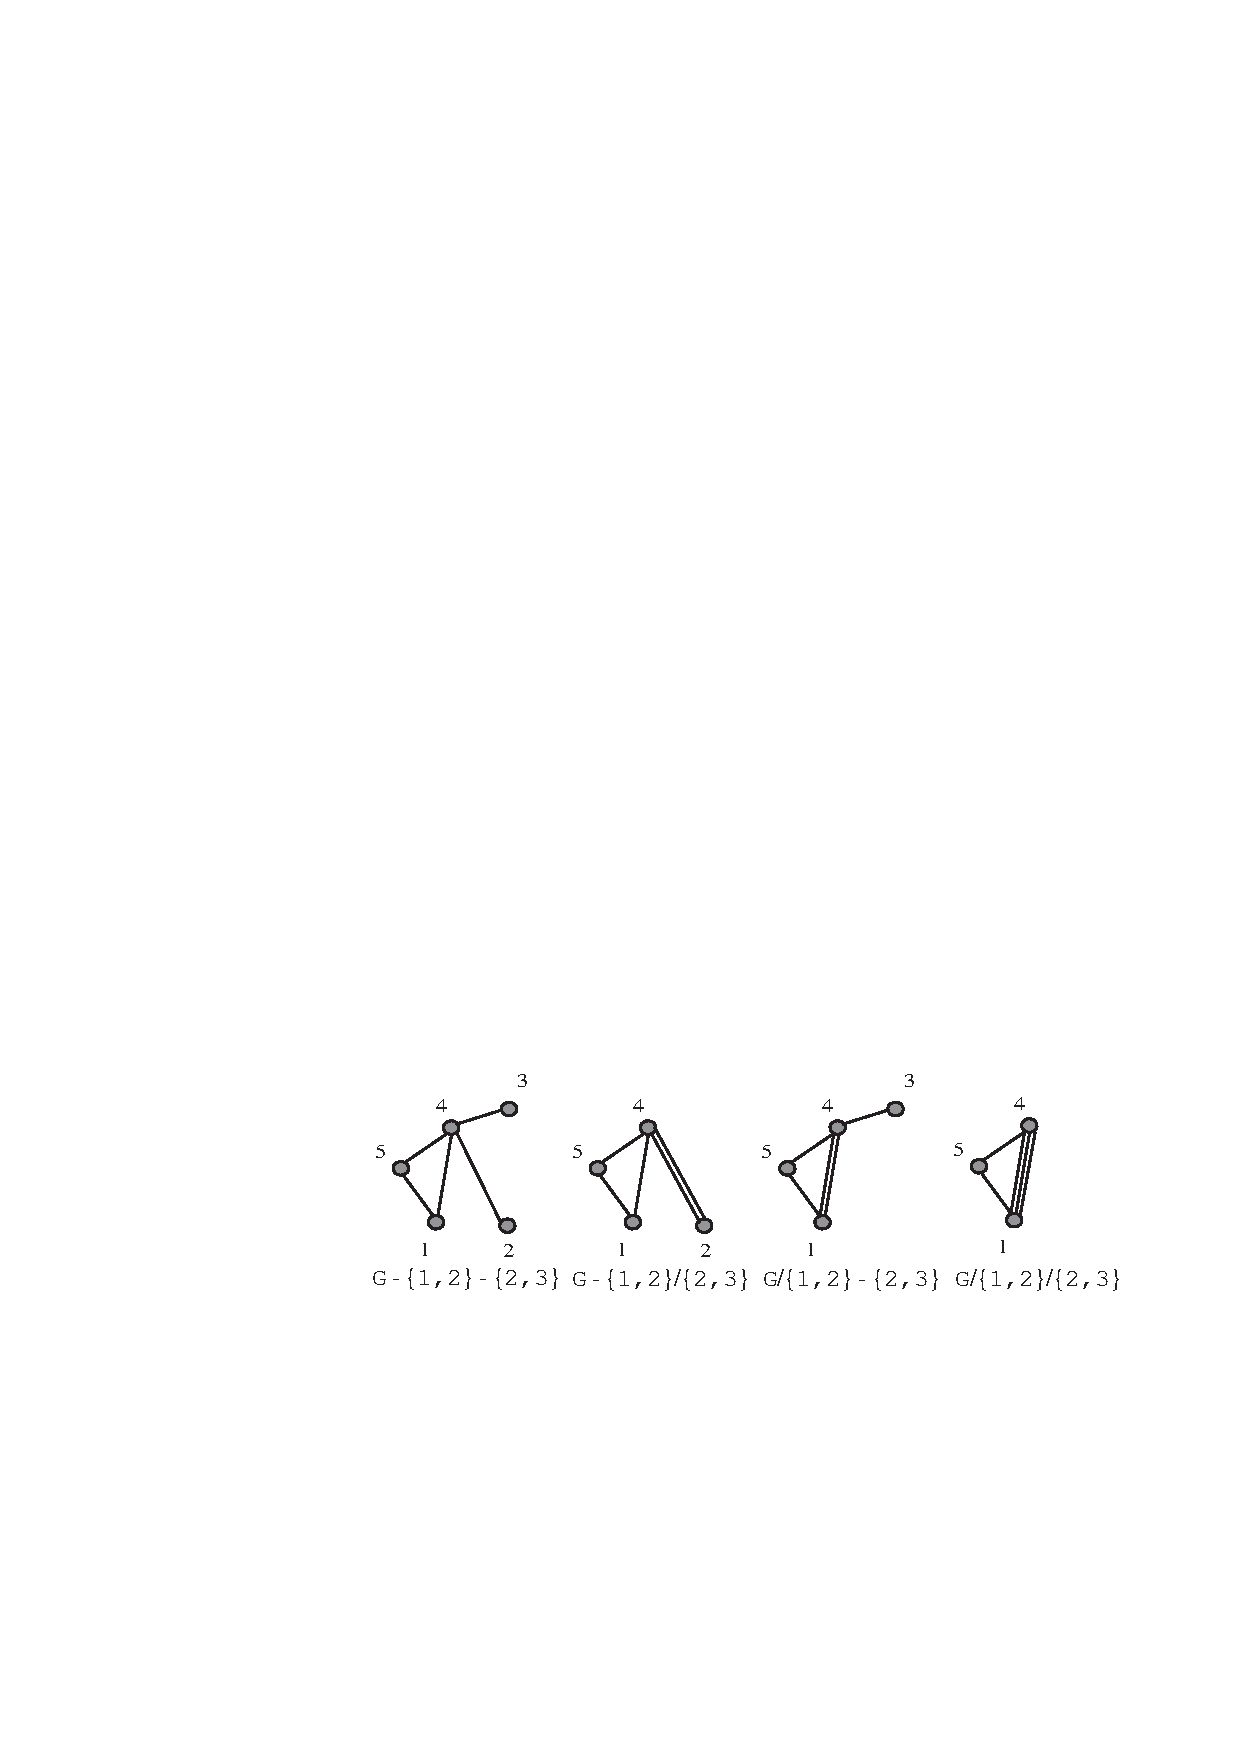
\includegraphics[width=0.95\linewidth]{images/spantreeexerciseresult}
\caption{Various deletions and contractions.\label{spantreeexerciseresult}}
\end{figure}
We could now convert each of these graphs to trees with multiple edges by deleting and contracting one more edge, say edge \(\{1,5\}\), which would make the analysis easier but the picture twice as big. Since we can easily count spanning trees of a triangle, we can also stop here, noting that the first graph has three spanning trees, the second has six, the third has five, and the fourth has seven, so the total number of spanning trees is \(3+6+5+7=21\).%
\end{activity}
\typeout{************************************************}
\typeout{Subsection  Shortest paths in graphs}
\typeout{************************************************}
\subsection[{Shortest paths in graphs}]{Shortest paths in graphs}\label{subsection-27}
Suppose that a company has a main office in one city and regional offices in other cities. Most of the communication in the company is between the main office and the regional offices, so the company wants to find a spanning tree that minimizes not the total cost of all the edges, but rather the cost of communication between the main office and each of the regional offices. It is not clear that such a spanning tree even exists. This problem is a special case of the following. We have a connected graph with nonnegative numbers assigned to its edges. (In this situation these numbers are often called weights.) The \emph{(weighted) length}\index{path!length of}\index{length (of a path)} of a path in the graph is the sum of the weights of its edges. The \emph{distance}\index{distance in a weighted graph}\index{graph!distance in} between two vertices is the least (weighted) length of any path between the two vertices. Given a vertex \(v\), we would like to know the distance between \(v\) and each other vertex, and we would like to know if there is a spanning tree in \(G\) such that the length of the path in the spanning tree from \(v\) to each vertex \(x\) is the distance from \(v\) to \(x\) in \(G\).%
\begin{activity}[]\label{Dijkstra}
Show that the following algorithm (known as Dijkstra's\index{Dijkstra's algorithm}\index{distance in a graph} algorithm) applied to a weighted graph whose vertices are labelled 1 to \(n\) gives, for each \(i\), the distance from vertex 1 to i as \(d(i)\). \leavevmode%
\begin{enumerate}
\item\hypertarget{li-34}{}Let \(d(1) = 0\). Let \(d(i) = \infty\) for all other \(i\).  Let \(v(1)\)=1. Let \(v(j) = 0\) for all other \(j\).  For each \(i\) and \(j\), let \(w(i,j)\) be the minimum weight of an edge between \(i\) and \(j\), or \(\infty\) if there are no such edges.  Let \(k=1\).  Let \(t=1\).%
\item\hypertarget{li-35}{}For each \(i\), if \(d(i)>d(k) + w(k,i)\) let \(d(i)= d(k) +w(k,i)\).%
\item\hypertarget{li-36}{}Among those \(i\) with \(v(i)=0\), choose one with \(d(i)\) a minimum, and let \(k=i\).  Increase \(t\) by 1. Let \(v(i) =1.\)%
\item\hypertarget{li-37}{}Repeat the previous two steps until \(t=n\)%
\end{enumerate}
%
\par\medskip\noindent%
\textbf{Solution.}\quad We prove that the distance from vertex 1 of a vertex \(i\) with \(v(i)=1\) is \(d(i)\). We use induction on the number \(t\) of vertices with \(v(i)=1\). If \(t=1\), then \(d(1)=0\) is the distance from vertex 1 to vertex 1. Now when \(t=s-1\), we have vertices \(i_1\), \(i_2\), \dots{} \(i_{s-1}\) such that \(v(i_p)=1\). Suppose inductively that \(d(i_p)\) is the distance from vertex \(i_p\) to vertex 1 for \(p=1,2,\ldots,s-1\). When \(t=s\), we choose a vertex \(i\) with \(d(i)\) a minimum. Suppose \(u_1,u_2,\ldots, u_r\) is the sequence of vertices of a shortest (least total weight) path from vertex \(u_1=1\) to vertex \(u_r=i\) and that the length (total weight) of this path is less than \(d(i)\). Suppose that some vertex \(u_p\) has \(v(u_p)=0\), and choose the smallest \(p\) such that this is so. Then \(d(u_{p-1})\) is the distance from vertex \(1\) to vertex \(u_{p-1}\), and \(d(u_{p-1}) + w(u_{p-1},u_p)\) is less than \(d(i)\) because the length of the path from \(u_1\) to \(u_r\) is less than \(d(i)\). Then we would not have chosen the vertex \(i\) after all, but rather the vertex \(u_p\), which is a contradiction, so all the vertices \(u_p\) with \(p\lt r\) must have \(v(u_p)=1\), and, by our inductive hypothesis, \(d(u_p)\) must be the distance from vertex 1 to vertex \(u_p\) for \(p\lt r\). Thus when we were computing \(d(i)\), we would have found that \(d(i)\le d(u_{r-1}) +w(u_{r-1},i)\). Thus \(d(i)\) must be the distance from vertex 1 to vertex \(i\) after all. Therefore the fact that Dijkstra's algorithm works when \(t=s-1\) implies that it works when \(t=s\), so that, by the principle of mathematical induction, it works for all nonnegative integers \(t\).%
\end{activity}
\begin{activity}[]\label{activity-111}
Is there a spanning tree such that the distance from vertex \(1\) to vertex \(i\) given by the algorithm in \hyperref[Dijkstra]{Problem~\ref{Dijkstra}} is the distance for vertex 1 to vertex \(i\) in the tree (using the same weights on the edges, of course)?%
\par\medskip\noindent%
\textbf{Solution.}\quad Yes, when we choose the \(i\) with \(d(i)\) a minimum, before we change \(k\) to \(i\), we add an edge from vertex \(k\) to vertex \(i\) to the edge set of a graph on the vertex set \([n]\). We get a tree each time we do this step, because we are adding a vertex of degree 1 to a smaller tree. We essentially proved in the solution to \hyperref[Dijkstra]{Problem~\ref{Dijkstra}} that the path from vertex 1 to vertex \(i\) in this tree has length (total weight) \(d(i)\). Using the same approach we could prove it directly by induction on the number of vertices in our tree.%
\end{activity}
\typeout{************************************************}
\typeout{Section 1.4 Supplementary Problems}
\typeout{************************************************}
\section[{Supplementary Problems}]{Supplementary Problems}\label{sec_induction-suppprobs}
\leavevmode%
\begin{enumerate}
\item\hypertarget{li-38}{}Use the inductive definition of \(a^n\) to prove that \((ab)^n=a^nb^n\) for all nonnegative integers \(n\). If \(n=0\) we get \((ab)^0=1\) and \(a^0b^0=1\). Assume inductively that \((ab)^{n-1}=a^{n-1}b^{n-1}\). Then by the inductive definition, inductive hypothesis, and commutative law,%
\begin{equation*}
(ab)^n= (ab)^{n-1}ab=a^{n-1}b^{n-1}ab=a^{n-1}ab^{n-1}b=a^nb^n.
\end{equation*}
%
\par
Thus the fact that \((ab)^{n-1}=a^{n-1}b^{n-1}\) implies the fact that \((ab)^n=
a^nb^n\). Therefore by the principle of mathematical induction, \((ab)^n=a^nb^n\) for all nonnegative integers \(n\).%
%
\item\hypertarget{li-39}{}Give an inductive definition of \(\displaystyle \bigcup_{i=1}^nS_i\) and use it and the two set distributive law to prove the distributive law \(\displaystyle{A\cap \bigcup_{i=1}^n S_i=\bigcup_{i=1}^n A\cap S_i}\). We define \(\displaystyle\bigcup_{i=1}^1S_i= S_i\) and \(\displaystyle
\bigcup_{i=1}^n S_i =
\bigcup_{i=1}^{n-1}S_i
\cup S_n\). Then%
\begin{equation*}
\displaystyle A\cap\bigcup_{i=1}^1S_i=
A\cap S_1=\bigcup_{i=1}^1 A\cap S_i.
\end{equation*}
%
\par
Assume that \(n>1\) and \(\displaystyle A\cap\bigcup_{i=1}^{n-1}=\bigcup_{i=1}^{n-1}A\cap S_i\). Now%
\begin{align*}
A\cap\bigcup_{i=1}^nS_i \amp =\amp  A\cap\left(\bigcup_{i=1}^{n-1}S_i
\cup S_n\right)=\left(A\cap\bigcup_{i=1}^{n-1}S_i\right) \cup\left( A\cap
S_n\right)\\
\amp =\amp \left(\bigcup_{i=1}^{n-1}A\cap
S_i\right)\cup\left(A\cap S_n\right)=\bigcup_{i=1}^n A\cap S_i.
\end{align*}
%
\par
Thus the truth of the distributive law for distributing an intersection over a union of \(n-1\) sets implies its truth for distributing an intersection over a union of \(n\) sets. Therefore by the principle of mathematical induction, the distributive law \(\displaystyle A\cap\bigcup_{i=1}^nS_i=
\bigcup_{i=1}^nA\cap S_i\) holds for all positive integers \(n\).%
%
\item\hypertarget{li-40}{}(interesting) A hydrocarbon molecule is a molecule whose only atoms are either carbon atoms or hydrogen atoms.  In a simple molecular model of a hydrocarbon, a carbon atom will bond to exactly four other atoms and hydrogen atom will bond to exactly one other atom.  We represent a hydrocarbon compound with a graph whose vertices are labelled with C's and H's so that each C vertex has degree four and each H vertex has degree one.  A hydrocarbon is called an ``alkane'' (common examples are methane (natural gas), propane, hexane (ordinary gasoline), octane (to make gasoline burn more slowly), etc.) if the graph is a tree.  How many vertices are labelled \(H\) in the graph of an alkane with exactly \(n\) vertices labelled \(C\)? We have \(n\) vertices of degree four, and so if we have \(m\) vertices of degree 1, we get \(4n+m=2(m+n-1)\) from the fact that the sum of the degrees of the vertices must be twice the number of edges. Thus we have \(m=2n+2\) hydrogen atoms.%
%
\item\hypertarget{li-41}{}%
\begin{enumerate}
\item\hypertarget{li-42}{}Give a recurrence for the number of ways to divide \(2n\) people into sets of two for tennis games.  (Don't worry about who serves first.) \(t_{2n}=(2n-1)t_{2n-2}\)%
%
\item\hypertarget{li-43}{}(interesting) Give a recurrence for the number of ways to divide \(4n\) people into sets of four for games of bridge.  (Don't worry about how they sit around the bridge table or who is the first dealer.) \(b_{4n}=\binom{4n-1}{3}b_{4n-4}\).%
%
\end{enumerate}
%
\item\hypertarget{li-44}{}Use induction to prove your result in Supplementary \hyperlink{composition_numberof}{Problem~2} at the end of Chapter 1. A composition of \(n\) is an ordered list of positive numbers that adds to \(n\). We wish to show that there are \(2^{n-1}\) compositions of \(n\). There is one composition of the number 1, and \(2^{1-1}=1\). Now assume inductively that there are \(2^{n-2}\) compositions of the number \({n-1}\). From a composition of \(n-1\), we can get a composition of \(n\) either by making a new last part of size 1, or by adding one to the last part. Clearly these two operations give different partitions of \(n\); what is not so clear is that they give all partitions of \(n\), but they do: Either the last part of a partition of \(n\) is 1, in which case it comes from the first kind of operation, or it is larger than one, in which case it comes from the second operation. Thus the number of compositions of \(n\) is twice the number of compositions of \(n-1\), and so is \(2\cdot2^{n-2}=2^{n-1}\). Therefore the statement that there are \(2^{n-2}\) compositions of \(n-1\) implies the statement that there are \(2^{n-1}\) compositions of \(n\). Thus by the principle of mathematical induction, there are \(2^{n-1}\) compositions of \(n\) for every positive integer \(n\).%
%
\item\hypertarget{inductiveprodnotation}{}Give an inductive definition of the product notation \(\displaystyle
\prod_{i=1}^n a_i\). \(\displaystyle\prod_{i=1}^1a_i=a_1\), and \(\displaystyle\prod_{i=1}^n
a_i= \left(\prod_{i=1}^{n-1}a_i\right)\cdot a_n\).%
%
\item\hypertarget{li-46}{}Using the fact that \((ab)^k =a^kb^k\), use your inductive definition of product notation in \hyperlink{inductiveprodnotation}{Problem~6} to prove that \(\displaystyle \left(\prod_{i=1}^n a_i\right)^k=\prod_{i=1}^n a_i^k\). When \(n=1\) we get \(\displaystyle\left(\prod_{i=1}^1 a_i\right)^k=
a_i^k =\prod_{i=1}^1a_i^k\). Now assume inductively that \(\displaystyle\left(\prod_{i=1}^{m-1}a_i\right)^k=\prod_{i=1}^{m-1}a_i^k\). Then we may write%
\begin{equation*}
\left(\prod_{i=1}^ma_i\right)^k=\left(\left(\prod_{i=1}^{m-1}
a_i\right)\cdot a_m\right)^k=\left(\prod_{i=1}^{m-1}
a_i^k\right)\cdot a_m^k=\prod_{i=1}^m a_i^k.
\end{equation*}
%
\par
Thus the correctness of the formula for \(n=m-1\) implies its correctness for \(n=m\). Therefore by the principle of mathematical induction, the formula holds for all positive integers \(n\).%
%
\item\hypertarget{li-47}{}(interesting) How many labelled trees on \(n\) vertices have exactly four vertices of degree 1? The vertices of degree 1 are the vertices that do not appear in the Grey code for the tree. So we first choose four vertices out of \(n\) in \(\binom{n}{4}\) ways to be our vertices of degree 1, and then we use the remaining \(n-4\) vertices to fill in our list of \(n-2\) vertices, using each of the \(n-4\) at least once. Thus we either use one of them 3 times and the rest once, or two of them twice and the rest once. There are \(n-4\) ways to choose the one we use three times and \(\binom{n-2}{3}\binom{n-5}{1}\binom{n-6}{1}\cdots\binom{1}{1}={(n-2)!\over3!}\) ways to label the \(n-2\) places with the chosen vertices. There are \(\binom{n-4}{2}\) ways to choose the vertices we would use twice, and \(\binom{n-2}{2}\binom{n-4}{2}\binom{n-6}{1}\binom{n-7}{1}\cdots \binom{1}{1}={(n-2)!\over 2!2!}\) ways to assign the chosen vertices to the \(n-2\) places in the Prüfer Code. Thus we have%
\begin{align*}
\amp \amp \binom{n}{4}\left((n-4){(n-2)!\over 3!} +{(n-4)(n-3)\over
2}{(n-2)!\over 4}\right)\\
\amp =\amp {n!\over 48}(n-2)^{\underline{3}}\left({1\over3} +{n-3\over 4}\right)
\end{align*}
possible Prüfer codes and therefore the same number of labelled trees.%
%
\item\hypertarget{li-48}{}(interesting and difficult) The degree sequence of a tree is a list of the degrees of the vertices in nonincreasing order.  For example the degree sequence of the first graph in \hyperref[spanningtrees]{Figure~\ref{spanningtrees}} is 43221.  How many labelled trees are there on \(n\) vertices with degree sequence \(d_1,d_2,\ldots d_n\), or, equivalently, with the degree sequence in which the degree \(d\) appears \(i_d\) times? We first solve the simpler problem in which we assume \(d_i\) is the degree of vertex \(i\). The number of times \(i\) appears in the Prüfer code of a tree is one less than the degree of \(i\), so vertex \(i\) appears \(d_i-1\) times. Thus the sum of the \(d_i-1\) should be \(2n-2-n=n-2\). Of the \(n-2\) places in the Prüfer code, we want to label \(d_1-1\) of them with 1, \(d_2-1\) of them with 2 and in general \(d_i-1\) of them with \(i\). There are%
\begin{equation*}
\binom{n-2}{d_1-1}\binom{n-2-(d_1-1)}{d_2-1}\binom{n-2-(d_1-1+d_2-1)}{d_3-1}\cdots\binom{d_n-1}{d_n-1}
\end{equation*}
ways to do this, so the number of trees in which vertex \(i\) has degree \(d_i\) is \({(n-2)!\over
(d_1-1)!(d_2-1)!\cdots(d_n-1)!}\).%
\par
Now we modify the solution by observing that to count all graphs with a given degree sequence, the actual vertices which have the given degrees is irrelevant, so we must multiply the result of the easier problem by the number of ways to assign the degrees to the vertices. To assign the degrees, we can list the vertices in \(n!\) ways, choose the first \(i_1\) of these vertices to have degree 1, then next \(i_2\) to have degree 2, and so on. But the order in which we list the vertices of a given degree is irrelevant. Thus the number of ways to assign the degrees is \(n!\over i_1!i_2!\cdots i_n!\). Once the degrees are assigned, there are \((n-2)!\over
\prod_{d=1}^n (d-1)!^{i_d}\), by translating our easier result. Thus the total number of trees with the degree sequence in which there are \(i_d\) vertices of degree \(d\) is%
\begin{equation*}
n!(n-2)!\over\prod_{j=1}^n i_j!(j-1)!^{i_j}.
\end{equation*}
%
%
\end{enumerate}
\typeout{************************************************}
\typeout{Chapter 2 Distribution Problems}
\typeout{************************************************}
\chapter[{Distribution Problems}]{Distribution Problems}\label{chapter-3}
\typeout{************************************************}
\typeout{Section 2.1 The idea of a distribution}
\typeout{************************************************}
\section[{The idea of a distribution}]{The idea of a distribution}\label{section-9}
\typeout{************************************************}
\typeout{Introduction  }
\typeout{************************************************}
Many of the problems we solved in Chapter 1 may be thought of as problems of distributing objects (such as pieces of fruit or ping-pong balls) to recipients (such as children). Some of the ways of viewing counting problems as distribution problems are somewhat indirect. For example, in \hyperref[ping-pong]{Problem~\ref{ping-pong}} you probably noticed that the number of ways to pass out \(k\) ping-pong balls to \(n\) children so that no child gets more than one is the number of ways that we may choose a \(k\)-element subset of an \(n\)-element set. We think of the children as recipients and objects we are distributing as the identical ping-pong balls, distributed so that each recipient gets at most one ball. Those children who receive an object are in our set. It is helpful to have more than one way to think of solutions to problems. In the case of distribution problems, another popular model for distributions is to think of putting balls in boxes rather than distributing objects to recipients. Passing out identical objects is modeled by putting identical balls into boxes. Passing out distinct objects is modeled by putting distinct balls into boxes.%
\typeout{************************************************}
\typeout{Subsection  The twenty-fold way}
\typeout{************************************************}
\subsection[{The twenty-fold way}]{The twenty-fold way}\label{subsection-28}
When we are passing out objects to recipients, we may think of the objects as being either identical or distinct. We may also think of the recipients as being either identical (as in the case of putting fruit into plastic bags in the grocery store) or distinct (as in the case of passing fruit out to children). We may restrict the distributions to those that give at least one object to each recipient, or those that give exactly one object to each recipient, or those that give at most one object to each recipient, or we may have no such restrictions. If the objects are distinct, it may be that the order in which the objects are received is relevant (think about putting books onto the shelves in a bookcase) or that the order in which the objects are received is irrelevant (think about dropping a handful of candy into a child's trick or treat bag). If we ignore the possibility that the order in which objects are received matters, we have created \(2\cdot2\cdot4=16\) distribution problems. In the cases where a recipient can receive more than one distinct object, we also have four more problems when the order objects are received matters. Thus we have 20 possible distribution problems.%
\begin{table}
\centering
\begin{tabular}{lll}
&&\tabularnewline\hrulethin
The Twentyfold Way: A Table of Distribution Problems\tabularnewline[0pt]
&&\tabularnewline\hrulemedium
\(k\) objects and conditions&\(n\) recipients and mathematical model for distribution\tabularnewline[0pt]
on how they are received&Distinct&Identical\tabularnewline[0pt]
&&\tabularnewline\hrulemedium
1.  Distinct&\(n^k\)&?\tabularnewline[0pt]
no conditions&functions&set partitions (\(\le n\) parts)\tabularnewline[0pt]
&&\tabularnewline\hrulethin
2.  Distinct&\(n^{\underline{k}}\)&1 if \(k\le n\); 0 otherwise\tabularnewline[0pt]
Each gets at most one&\kern -2pt \(k\)-element permutations\kern -2 pt&\tabularnewline[0pt]
&&\tabularnewline\hrulethin
3.  Distinct&?&?\tabularnewline[0pt]
Each gets at least one&onto functions&set partitions (\(n\) parts)\tabularnewline[0pt]
&&\tabularnewline\hrulethin
4. Distinct&\(k!=n!\)&1 if \(k=n\); 0 otherwise\tabularnewline[0pt]
Each gets exactly one&bijections&\tabularnewline[0pt]
&&\tabularnewline\hrulethin
5.  Distinct, order matters&?&?\tabularnewline[0pt]
&?&?\tabularnewline[0pt]
&&\tabularnewline\hrulethin
6.  Distinct, order matters&?&?\tabularnewline[0pt]
Each gets at least one&?&?\tabularnewline[0pt]
&&\tabularnewline\hrulethin
7.  Identical&?&?\tabularnewline[0pt]
no conditions&?&?\tabularnewline[0pt]
&&\tabularnewline\hrulethin
8.  Identical&\(\binom{n}{k}\)&1 if \(k\le n\); 0 otherwise\tabularnewline[0pt]
Each gets at most one&subsets&\tabularnewline[0pt]
&&\tabularnewline\hrulethin
9.  Identical&?&?\tabularnewline[0pt]
Each gets at least one&?&?\tabularnewline[0pt]
&&\tabularnewline\hrulethin
10.  Identical&1 if \(k=n\); 0 otherwise&1 if \(k=n\); 0 otherwise\tabularnewline[0pt]
Each gets exactly one&&\tabularnewline[0pt]
&&\tabularnewline\hrulethin
\end{tabular}
\caption{An incomplete table of the number of ways to distribute \(k\) objects to \(n\) recipients, with restrictions on how the objects are received\label{firstdistributiontable}}
\end{table}
We describe these problems in \hyperref[firstdistributiontable]{Table~\ref{firstdistributiontable}}. Since there are twenty possible distribution problems, we call the table the ``Twentyfold Way,''\index{Twentyfold Way} adapting terminology suggested by Joel Spencer for a more restricted class of distribution problems. In the first column of the table we state whether the objects are distinct (like people) or identical (like ping-pong balls) and then give any conditions on how the objects may be received. The conditions we consider are whether each recipient gets at most one object, whether each recipient gets at least one object, whether each recipient gets exactly one object, and whether the order in which the objects are received matters. In the second column we give the solution to the problem and the name of the mathematical model for this kind of distribution problem when the recipients are distinct, and in the third column we give the same information when the recipients are identical. We use question marks as the answers to problems we have not yet solved and models we have not yet studied. We give explicit answers to problems we solved in {$\langle\langle$Unresolved xref, reference "whatis"; check spelling or use "provisional" attribute$\rangle\rangle$} and problems whose answers are immediate. The goal of this chapter is to develop methods that will allow us to fill in the table with formulas or at least quantities we know how to compute, and we will give a completed table at the end of the chapter. We will now justify the answers that are not question marks and replace some question marks with answers as we cover relevant material.%
\par
If we pass out \(k\) distinct objects (say pieces of fruit) to \(n\) distinct recipients (say children), we are saying for each object which recipient it goes to. Thus we are defining a function from the set of objects to the recipients. We saw the following theorem in \hyperref[numberoffunctionsconjecture]{Problem~}.%
\begin{theorem}[{}]\label{theorem-3}
There are \(n^k\)\index{functions!number of} functions from a \(k\)-element set to an \(n\)-element set.%
\end{theorem}
We proved it in {$\langle\langle$Unresolved xref, reference "provenumberoffunctionsconjecture"; check spelling or use "provisional" attribute$\rangle\rangle$}. If we pass out \(k\) distinct objects (say pieces of fruit) to \(n\) indistinguishable recipients (say identical paper bags) then we are dividing the objects up into disjoint sets; that is we are forming a partition of the objects into some number, certainly no more than the number \(k\) of objects, of parts. Later in this chapter (and again in the next chapter) we shall discuss how to compute the number of partitions of a \(k\)-element set into \(n\) parts. This explains the entries in row one of our table.%
\par
If we pass out \(k\) distinct objects to \(n\) recipients so that each gets at most one, we still determine a function, but the function must be one-to-one. The number of one-to-one functions from a \(k\)-element set to an \(n\) element set is the same as the number of one-to-one functions from the set \([k] =\{1,2,\ldots,k\}\) to an \(n\)-element set. In \hyperref[kelementpermutation]{Problem~\ref{kelementpermutation}} we proved the following theorem.%
\begin{theorem}[{}]\label{numberofinjections}
If \(0\le k\le n\), then the number of \(k\)-element permutations of an \(n\)-element set is%
\begin{equation*}
n^{\underline{k}} = n(n-1)\cdots(n-k+1) =
n!/(n-k)!.
\end{equation*}
%
\par
\index{functions!one-to-one!number of}%
\end{theorem}
If \(k>n\) there are no one-to-one functions from a \(k\) element set to an \(n\) element, so we define \(n^{\underline{k}}\) to be zero in this case. Notice that this is what the indicated product in the middle term of our formula gives us. If we are supposed to distribute \(k\) distinct objects to \(n\) identical recipients so that each gets at most one, we cannot do so if \(k>n\), so there are 0 ways to do so. On the other hand, if \(k\le n\), then it doesn't matter which recipient gets which object, so there is only one way to do so. This explains the entries in row two of our table.%
\par
If we distribute \(k\) distinct objects to \(n\) distinct recipients so that each recipient gets at least one, then we are counting functions again, but this time functions from a \(k\)-element set \emph{onto} an \(n\)-element set. At present we do not know how to compute the number of such functions, but we will discuss how to do so later in this chapter and in the next chapter. If we distribute \(k\) identical objects to \(n\) recipients, we are again simply partitioning the objects, but the condition that each recipient gets at least one means that we are partitioning the objects into exactly \(n\) blocks. Again, we will discuss how compute the number of ways of partitioning a set of \(k\) objects into \(n\) blocks later in this chapter. This explains the entries in row three of our table.%
\par
If we pass out \(k\) distinct objects to \(n\) recipients so that each gets exactly one, then \(k=n\) and the function that our distribution gives us is a bijection. The number of bijections from an \(n\)-element set to an \(n\)-element set is \(n!\) by \hyperref[numberofinjections]{Theorem~\ref{numberofinjections}}. If we pass out \(k\) distinct objects of \(n\) identical recipients so that each gets exactly 1, then in this case it doesn't matter which recipient gets which object, so the number of ways to do so is 1 if \(k=n\). If \(k\not=n\), then the number of such distributions is zero. This explains the entries in row four of our table.%
\par
We now jump to row eight of our table. We saw in \hyperref[ping-pong]{Problem~\ref{ping-pong}} that the number of ways to pass out \(k\) identical ping-pong balls to \(n\) children is simply the number of \(k\)-element subsets of an \(n\)-element set. In \hyperref[formulanchoosek]{Problem~\ref{formulanchoosek}} we proved the following theorem.%
\begin{theorem}[{}]\label{theorem-5}
If \(0\le k \le n\), the number of \(k\)-element subsets of an \(n\)-element set is given by%
\begin{equation*}
\binom{n}{k} = {n^{\underline{k}}\over k!}
= {n!\over k!(n-k)!}.
\end{equation*}
%
\end{theorem}
We define \(\binom{n}{k}\) to be 0 if \(k>n\), because then there are no \(k\)-element subsets of an \(n\)-element set. Notice that this is what the middle term of the formula in the theorem gives us. This explains the entries of row 8 of our table. For now we jump over row 9.%
\par
In row 10 of our table, if we are passing out \(k\) identical objects to \(n\) recipients so that each gets exactly one, it doesn't matter whether the recipients are identical or not; there is only one way to pass out the objects if \(k=n\) and otherwise it is impossible to make the distribution, so there are no ways of distributing the objects. This explains the entries of row 10 of our table. Several other rows of our table can be computed using the methods of Chapter 1.%
\typeout{************************************************}
\typeout{Subsection  Ordered functions}
\typeout{************************************************}
\subsection[{Ordered functions}]{Ordered functions}\label{orderedfunctionsection}
\begin{activity}[]\label{bookcase}
~\par
\begin{enumerate}[label=(\alph*)]
 \item Suppose we wish to place \(k\) distinct books onto the shelves of a bookcase with \(n\) shelves. For simplicity, assume for now that all of the books would fit on any of the shelves. Also, let's imagine pushing the books on a shelf as far to the left as we can, so that we are only thinking about how the books sit relative to each other, not about the exact places where we put the books. Since the books are distinct, we can think of a the first book, the second book and so on. How many places are there where we can place the first book? When we place the second book, if we decide to place it on the shelf that already has a book, does it matter if we place it to the left or right of the book that is already there? How many places are there where we can place the second book? Once we have \(i-1\) books placed, if we want to place book \(i\) on a shelf that already has some books, is sliding it in to the left of all the books already there different from placing it to the right of all the books already or between two books already there? In how many ways may we place the \(i\)th book into the bookcase? In how many ways may we place all the books?%
\par\medskip\noindent%
\textbf{Solution.}\quad There are \(n\) places where we can place the first book. Once we have placed it, there are \(n+1\) places where we can place the second book, because on the shelf that has one book, we could put the second book to the left or to the right of the book already there. Once we have \(i-1\) books on the shelves the \(i\)th book could go on any shelf to the left of all books there, if any, giving us \(n\) places, or it could go to the immediate right of any book already there, giving us another \(i-1\) places. Thus there are \(n+i-1\) places where we could place book \(i\). From this, we can see that the number of ways to place all the books is%
\begin{equation*}
\prod_{i=1}^k (n+i-1).
\end{equation*}
%

~\par
\item Suppose we wish to place the books in \hyperref[bookcase]{Problem~\ref{bookcase}} (satisfying the assumptions we made there) so that each shelf gets at least one book. Now in how many ways may we place the books? (Hint: how can you make sure that each shelf gets at least one book before you start the process described in \hyperref[bookcase]{Problem~\ref{bookcase}}?)%
\par\medskip\noindent%
\textbf{Solution.}\quad Choose \(n\) books from the \(k\) books in \(\binom{k}{n}\) ways, and assign them to the \(n\) places shelves in \(n!\) ways, giving us \(k!/(k-n)!\) ways to put a book on each shelf. Now leaving these books at the far left of each shelf, place the remaining books in%
\begin{equation*}
\prod_{i=1}^{k-n}
(n+i-1)={(n+(k-n)-1)!\over (n-1)!}={(k-1)!\over (n-1)!}
\end{equation*}
ways. Thus we have%
\begin{equation*}
{k!(k-1)!\over(k-n)!(n-1)!}=k!\binom{k-1}{n-1}
\end{equation*}
ways to place the books. Of course the right hand side of that equation cries out for a combinatorial explanation. Here it is. Imagine lining up the \(k\) books in a row. Then there are \(k-1\) places in between them. Choose \(n-1\) of these places, and slide a piece of paper in there as a divider. Now put the books before the first divider on shelf one, and the books after divider \(i\) on shelf \(i+1\). This gives an arrangement of the books on the shelves so that every shelf has a book!%

\end{enumerate}
\end{activity}
The assignment of which books go to which shelves of a bookcase is simply a function from the books to the shelves. But a function doesn't determine which book sits to the left of which others on the shelf, and this information is part of how the books are arranged on the shelves. In other words, the order in which the shelves receive their books matters.  Our function must thus assign an ordered list of books to each shelf. We will call such a function an ordered function. More precisely, an \terminology{ordered function}\index{ordered function}\index{function!ordered} from a set \(S\) to a set \(T\) is a function that assigns an (ordered) list of elements of \(S\) to some, but not necessarily all, elements of \(T\) in such a way that each element of \(S\) appears on one and only one of the lists.\footnote{The phrase ordered function is not a standard one, because there is as yet no standard name for the result of an ordered distribution problem.\label{fn-6}} (Notice that although it is not the usual definition of a function from \(S\) to \(T\), a function\index{function!alternate definition} can be described as an assignment of subsets of \(S\) to some, but not necessarily all, elements of \(T\) so that each element of \(S\) is in one and only one of these subsets.) Thus the number of ways to place the books into the bookcase is the entry in the middle column of row 5 of our table. If in addition we require each shelf to get at least one book, we are discussing the entry in the middle column of row 6 of our table. An \terminology{ordered onto function}\index{function!ordered!onto}\index{ordered onto function}\index{onto function!ordered} is one which assigns a list to each element of \(T\). In \hyperref[bookcase]{Problem~\ref{bookcase}} you showed that the number of ordered functions from a \(k\)-element set to an \(n\)-element set is \(\displaystyle \prod_{i=1}^n (n+i-1)\). This product occurs frequently enough that it has a name; it is called the \(k\)\/th \terminology{rising factorial power}\index{factorial power!rising}\index{rising factorial power} of \(n\) and is denoted by \(n^{\overline{k}}\).\index{\(n^{\overline{k}}\)} It is read as ``\(n\) to the \(k\) rising." (This notation is due to Don Knuth, who also suggested the notation for falling factorial powers.)\index{factorial} We can summarize with a theorem that adds two more formulas for the number of ordered functions.\index{factorial!falling}\index{falling factorial power}%
\begin{theorem}[{}]\label{theorem-6}
The number of ordered functions from a \(k\)-element set to an \(n\)-element set is%
\begin{equation*}
n^{\overline{k}}=\prod_{i=1}^n (n+i-1) = {(n+i-1)!\over (n-1)!} =
(n+k-1)^{\underline{k}}.
\end{equation*}
%
\end{theorem}
\typeout{************************************************}
\typeout{Subsection  Broken permutations and Lah numbers}
\typeout{************************************************}
\subsection[{Broken permutations and Lah numbers}]{Broken permutations and Lah numbers}\label{subsection-30}
\begin{activity}[]\label{brokenpermutation}
In how many ways may we stack \(k\) distinct books into \(n\) identical boxes so that there is a stack in every box? The hints may suggest that you can do this problem in more than one way!%
\par\medskip\noindent%
\textbf{Hint.}\quad Imagine taking a stack of \(k\) books, and breaking it up into stacks to put into the boxes in the same order they were originally stacked. If you are going to use \(n\) boxes, in how many places will you have to break the stack up into smaller stacks, and how many ways can you do this?%
\par\medskip\noindent%
\textbf{Hint.}\quad How many different bookcase arrangements correspond to the same way of stacking \(k\) books into \(n\) boxes so that each box has at least one book?%
\par\medskip\noindent%
\textbf{Solution.}\quad We can make a list of the \(k\) distinct books in \(k!\) ways. Then we have to choose \(n-1\) of the \(k-1\) places between the lists as the places where we will break the list. However the order in which we list the boxes is irrelevant, so we have equivalence classes of \(n!\) arrangements for each way of putting the books into boxes. Thus we can put the books in boxes in \(k!\binom{k-1}{n-1}/n!\) ways.%
\par
Alternately, we can take the number of ways to put \(k\) books onto \(n\) bookshelves so that each shelf gets at least one, and then divide by the number of shelves factorial. That gives us \(k!\binom{k-1}{n-1}/n!\) ways to arrange the books.%
\end{activity}
We can think of stacking books into identical boxes as partitioning the books and then ordering the blocks of the partition. This turns out not to be a useful computational way of visualizing the problem because the number of ways to order the books in the various stacks depends on the sizes of the stacks and not just the number of stacks. However this way of thinking actually led to the first hint in \hyperref[brokenpermutation]{Problem~\ref{brokenpermutation}}. Instead of dividing a set up into nonoverlapping parts, we may think of dividing a \emph{permutation} (thought of as a list) of our \(k\) objects up into \(n\) ordered blocks. We will say that a set of ordered lists of elements of a set \(S\) is a \terminology{broken permutation}\index{broken permutation}\index{permutation!broken} of \(S\) if each element of \(S\) is in one and only one of these lists.\footnote{The phrase broken permutation is not standard, because there is no standard name for the solution to this kind  of distribution problem.\label{fn-7}} The number of broken permutations of a \(k\)-element set with \(n\) blocks is denoted by \(L(k,n)\). The number \(L(k,n)\) is called a \terminology{Lah Number} and, from our solution to \hyperref[brokenpermutation]{Problem~\ref{brokenpermutation}}, is equal to \(k!\binom{k-1}{n-1}/n!\).\index{Lah number}%
\par
The Lah numbers are the solution to the question ``In how many ways may we distribute \(k\) distinct objects to \(n\) identical recipients if order matters and each recipient must get at least one?" Thus they give the entry in row 6 and column 6 of our table. The entry in row 5 and column 6 of our table will be the number of broken permutations with less than or equal to \(n\) parts. Thus it is a sum of Lah numbers.%
\par
We have seen that ordered functions and broken permutations explain the entries in rows 5 and 6 of our table.%
\typeout{************************************************}
\typeout{Subsection  Compositions of integers}
\typeout{************************************************}
\subsection[{Compositions of integers}]{Compositions of integers}\label{subsection-31}
\begin{activity}[]\label{activity-114}
In how many ways may we put \(k\) identical books onto \(n\) shelves if each shelf must get at least one book?%
\par\medskip\noindent%
\textbf{Solution.}\quad In {$\langle\langle$Unresolved xref, reference "bookcaseeveryshelf"; check spelling or use "provisional" attribute$\rangle\rangle$} we showed that with \(k\) distinct books we could place the books in \(k!\binom{k-1}{n-1}\) ways. We can partition these arangements of distinct books into blocks, where each block consists of all arrangements that we get just by permuting the books among themselves. Thus each block has \(k!\) arrangements in it, and each arrangement corresponds to an arrangement of identical books. Thus there are \(\binom{k-1}{n-1}\) ways to arrange identical books.%
\end{activity}
\begin{activity}[]\label{compositionagian}
A \terminology{composition} of the integer \(k\) into \(n\) parts is a list of \(n\) positive integers that add to \(k\).  How many compositions are there of an integer \(k\) into \(n\) parts?%
\par\medskip\noindent%
\textbf{Solution.}\quad There is a bijection between compositions of \(k\) into \(n\) parts and arrangements of \(k\) identical books on \(n\) shelves so that each shelf gets a book. Namely, the number of books on shelf \(i\) is the \(i\)th element of the list. Thus the number of compositions of \(k\) into \(n\) parts is \(\binom{k-1}{n-1}\).%
\end{activity}
\begin{activity}[]\label{activity-116}
Your answer in \hyperref[compositionagian]{Problem~\ref{compositionagian}} can be expressed as a binomial coefficient. This means it should be possible to interpret a composition as a subset of some set. Find a bijection between compositions of \(k\) into \(n\) parts and certain subsets of some set.  Explain explicitly how to get the composition from the subset and the subset from the composition.%
\par\medskip\noindent%
\textbf{Solution.}\quad If we line up \(k\) identical books, there are \(k-1\) places in between two books. If we choose \(n-1\) of these places and slip dividers into those places, then we have a first clump of books, a second clump of books, and so on. The \(i\)th element of our list is the number of books in the \(i\)th clump. Clearly using books is irrelevant; we could line up any \(k\) identical objects and make the same argument. Our bijection is between compositions and \((n-1)\)-element subsets of the set of \(k-1\) spaces between our objects.%
\end{activity}
\begin{activity}[]\label{activity-117}
Explain the connection between compositions of \(k\) into \(n\) parts and the problem of distributing \(k\) identical objects to \(n\) recipients so that each recipient gets at least one.%
\par\medskip\noindent%
\textbf{Solution.}\quad Since the recipients are distinct, we can think of them as a first recipient, a second, and so on. Given a composition of \(k\) into \(n\) parts, let the \(i\)th element of the list be the number of objects given to recipient number \(i\).%
\end{activity}
The sequence of problems you just completed should explain the entry in the middle column of row 9 of our table of distribution problems.%
\typeout{************************************************}
\typeout{Subsection  Multisets}
\typeout{************************************************}
\subsection[{Multisets}]{Multisets}\label{subsection-32}
In the middle column of row 7 of our table, we are asking for the number of ways to distribute \(k\) identical objects (say ping-pong balls) to \(n\) distinct recipients (say children).%
\begin{activity}[]\label{identicalbooks}
In how many ways may we distribute \(k\) identical books on the shelves of a bookcase with \(n\) shelves, assuming that any shelf can hold all the books?%
\par\medskip\noindent%
\textbf{Solution.}\quad We saw that we could arrange \(k\) distinct books on \(n\) shelves in \(\prod_{i=1}^k (n+i-1)\) ways. We partition these arrangements into blocks by putting two arrangements in the same block if we can get one from the other by permuting the books among themselves. Then the number of blocks is the number of ways to place identical books on the shelves. However, there are \(k!\) arrangements per block, so there are%
\begin{equation*}
{\prod_{i=1}^k (n+i-1)\over k!}=(n+k-1)^{\underline{k}}= \binom{n+k-1}{k}
\end{equation*}
ways to arrange identical books.%
\end{activity}
\begin{activity}[]\label{multiset}
A \terminology{multiset}\index{multiset} chosen from a set \(S\) may be thought of as a subset with repeated elements allowed. For example the multiset of letters of the word Mississippi is \(\{i,i,i,i,m,p,p,s,s,s,s\}\). To determine a multiset we must say how many times (including, perhaps, zero) each member of \(S\) appears in the multiset. The number of times an element appears is called its \terminology{multiplicity}.\index{multiplicity in a multiset} The size of a multiset chosen from \(S\) is the total number of times any member of \(S\) appears. For example, the size of the multiset of letters of Mississippi is 11. What is the number of multisets of size \(k\) that can be chosen from an \(n\)-element set?%
\par\medskip\noindent%
\textbf{Solution.}\quad There is a bijection between arrangements of identical books on \(n\) shelves and multisets chosen from an \(n\)-element set: the multiplicity of element \(i\) is the number of books on shelf \(i\). Thus we have \(\binom{n+k-1}{k}\) ways to choose a \(k\)-element multiset from an \(n\)-element set by \hyperref[identicalbooks]{Problem~\ref{identicalbooks}}.%
\end{activity}
\begin{activity}[]\label{activity-120}
~\par
\begin{enumerate}[label=(\alph*)]
 \item Your answer in the previous problem should be expressible as a binomial coefficient. Since a binomial coefficient counts subsets, find a bijection between subsets of something and multisets chosen from a set \(S\).%
\par\medskip\noindent%
\textbf{Solution.}\quad Note that \(\binom{n+k-1}{k} = \binom{n+k-1 }{n-1}\). We will show a bijection between ways of choosing \(n-1\) things our of \(n+k-1\) things and multisets. Namely, take \(n+k-1\) objects and line them up in a row. Choose \(n-1\) of them. Now let the multiplicity of element 1 of our multiset be the number of objects before the first thing we chose.  if \(1\lt i\lt n\), let the multiplicity of element \(i\) of our multiset be the number of things between the \(i-1\)th thing we chose and the \(i\)th thing we choose. Let the multiplicity of the \(n\)th element of our multiset be the number of objects after the last one we chose. Another way to say the essentially same thing is to make a list of \(n+k-1\) blank spaces. We choose \(k\) of them in which we put ones and \(n-1\) of them in which we put plus signs. Then the multiplicity of element 1 is the number of ones before the first plus sign, the multiplicity of element \(n\) is the number of ones after the last plus sign and if \(1\lt i\lt n\), the multiplicity of element \(i\) is the number of ones between the \((i-1)\)th plus sign and the \(i\)th plus sign.%

~\par
\item How many solutions are there in nonnegative integers to the equation \(x_1+x_2+ \cdots +x_m = r\), where \(m\) and \(r\) are constants?%
\par\medskip\noindent%
\textbf{Solution.}\quad We can think of \(x_i\) as the multiplicity of element \(i\) of a multiset chosen from among \(m\) things. The total number of elements of the multiset will be \(r\). Thus we have \(\binom{m+r-1}{r}\) solutions.%

\end{enumerate}
\end{activity}
A more precise definition of a \terminology{multiset}\index{multiset} chosen from a set \(S\) is that it is a function \(m\), called a \terminology{multiplicity function}\index{multiplicity function}, from \(S\) to the nonnegative integers. For each \(x\) in \(S\), \(m(x)\) specifies how many times \(x\) appears in the multiset. In our example of the word Mississippi above, our set \(S\) can be taken to be the set of alphabet letters and the multiplicity function \(m\) is given by \(m({ i})=4\), \(m({ m}) =1\), \(m({ p})=2\), \(m({ s}) =4\), and \(m\) of any other member of \(S\) is 0. When we list the members of a multiset in braces, it will be clear from context that we are thinking of a multiset. However when we use braces in another way, it may not be clear what we mean. For example, when we write%
\begin{equation*}
\{x|x \mbox{~is a letter of Mississippi} \},
\end{equation*}
do we mean the set \(\{i,m,p,s\}\) or the multiset \(\{i,i,i,i,m,p,p,s,s,s,s\}\)? To resolve this, whenever it is not clear from context whether we are talking about a set or multiset we will use the subscript multi on the right brace enclosing the multiset to distinguish a multiset. Thus we write%
\begin{equation*}
\{x|x \mbox{\ is a letter of
Mississippi} \}_{\mbox{\scriptsize multi} }=\{i,i,i,i,m,p,p,s,s,s,s\}.
\end{equation*}
%
\par
In this case it is probably clear from the right-hand side of the equation that we are thinking of the left-hand side as a multiset, but we will always try to err in the direction of clarity rather than brevity.%
\par
The sequence of problems you just completed should explain the entry in the middle column of row 7 of our table of distribution problems. In the next two sections we will give ways of computing the remaining entries.%
\typeout{************************************************}
\typeout{Section 2.2 Partitions and Stirling Numbers}
\typeout{************************************************}
\section[{Partitions and Stirling Numbers}]{Partitions and Stirling Numbers}\label{section-10}
\typeout{************************************************}
\typeout{Introduction  }
\typeout{************************************************}
We have seen how the number of partitions of a set of \(k\) objects into \(n\) blocks corresponds to the distribution of \(k\) distinct objects to \(n\) identical recipients. While there is a formula that we shall eventually learn for this number, it requires more machinery than we now have available. However there is a good method for computing this number that is similar to Pascal's equation. Now that we have studied recurrences in one variable, we will point out that Pascal's equation is in fact a \emph{recurrence in two variables}\index{recurrence!two variable}; that is it lets us compute \(\binom{n}{k}\) in terms of values of \(\binom{m}{i}\) in which either \(m\lt n\) or \(i\lt k\) or both. It was the fact that we had such a recurrence and knew \(\binom{n}{0}\) and \(\binom{n}{n}\) that let us create Pascal's triangle.%
\typeout{************************************************}
\typeout{Subsection  Stirling Numbers of the second kind}
\typeout{************************************************}
\subsection[{Stirling Numbers of the second kind}]{Stirling Numbers of the second kind}\label{subsection-33}
We use the notation \(S(k,n)\) to stand for the number of partitions of a \(k\) element set with \(n\) blocks. For historical reasons, \(S(k,n)\) is called a \emph{Stirling number of the second kind}. \index{partition!of a set}\index{partition!of a set!!Stirling Numbers}\index{Stirling Number!second kind}\index{\(S(k,n)\)}%
\begin{activity}[]\label{secondstirlingrecurrence}
~\par
\begin{enumerate}[label=(\alph*)]
 \item In a partition of the set \([k]\), the number \(k\) is either in a block by itself, or it is not. How does the number of partitions of \([k]\) with \(n\) parts in which \(k\) is in a block with other elements of \([k]\) compare to the number of partitions of \([k-1]\) into \(n\) blocks? Find a two variable recurrence for \(S(n,k)\), valid for \(n\) and \(k\) larger than one.%
\par\medskip\noindent%
\textbf{Solution.}\quad The number of partitions of \([k]\) into \(n\) parts in which \(k\) is in a block with other elements of \([k]\) is equal \(n\) times the number of partitions of \([k-1]\) into \(n\) blocks, because \(k\) could be in any of the \(n\) parts, and since it is in a block with other elements of \([k-1]\), removing it leaves a partition of \([k-1]\) into \(n\) blocks. The number of partitions of \([k]\) into \(n\) blocks in which \(k\) is in a block by itself is the number of partitions of \([k]\) into \(n-1\) blocks, because you can get any such partition in by deleting the block containing \(k\) from a partition of \([k]\) in which \(k\) is in a block by itself. Thus \(S(k,n))=S(k-1,n-1) +nS(k-1,n)\).%

~\par
\item What is \(S(k,1)\)? What is \(S(k,k)\)? Create a table of values of \(S(k,n)\) for \(k\) between 1 and 5 and \(n\) between 1 and \(k\). This table is sometimes called \terminology{Stirling's Triangle (of the second kind)}\index{Stirling's triangle!second kind} How would you define \(S(k,n)\) for the nonnegative values of \(k\) and \(n\) that are not both positive? Now for what values of \(k\) and \(n\) is your two variable recurrence valid?%
\par\medskip\noindent%
\textbf{Solution.}\quad \(S(k,1)=1\) and \(S(k,k)=1\).%
\begin{table}
\centering
\begin{tabular}{llllllll}
\(k\backslash n\)&0&1&2&3&4&5&6\tabularnewline[0pt]
&&&&&&&\tabularnewline\hrulethin
0&1&0&0&0&0&0&0\tabularnewline[0pt]
1&0&1&0&0&0&0&0\tabularnewline[0pt]
2&0&1&1&0&0&0&0\tabularnewline[0pt]
3&0&1&3&1&0&0&0\tabularnewline[0pt]
4&0&1&7&6&1&0&0\tabularnewline[0pt]
5&0&1&15&25&10&1&0
\end{tabular}
\caption{Stirling's Triangle of the second kind\label{stirling-triangle-second}}
\end{table}
As you see in the table, we define \(S(0,0)=1\), and \(S(0,n)\) or \(S(k,0)\) to be 0 otherwise. This makes sense because for \(n>0\) there is no partition of an empty set into \(n\) parts, and for \(k>0\) there is no partition of a \(k\)-element set into no parts, but saying there is one partition of the empty set into no parts allows us to use our recurrence to compute \(S(1,1)\).  This makes our recurrence valid for all nonnegative values of \(k\) and \(n\).%

~\par
\item Extend Stirling's triangle enough to allow you to answer the following question and answer it. (Don't fill in the rows all the way; the work becomes quite tedious if you do. Only fill in what you need to answer this question.) A caterer is preparing three bag lunches for hikers. The caterer has nine different sandwiches. In how many ways can these nine sandwiches be distributed into three identical lunch bags so that each bag gets at least one?%
\par\medskip\noindent%
\textbf{Solution.}\quad We need \(S(9,3)\). Thus we need to extend our table for four more rows, but only out to the column labelled 3. These rows are 6,0,1,31,90, 7,0,1,63,301, 7,0,1,127,966, 8,0,1,255,3025, 9,0,1,511,9330. Thus there are 9330 ways to distribute the sandwiches into the lunch bags.%

~\par
\item The question in {$\langle\langle$Unresolved xref, reference "sandwiches"; check spelling or use "provisional" attribute$\rangle\rangle$} naturally suggests a more realistic question; in how many ways may the caterer distribute the nine sandwich's into three identical bags so that each bag gets exactly three? Answer this question. (Hint, what if the question asked about six sandwiches and two distinct bags? How does having identical bags change the answer?)%
\par\medskip\noindent%
\textbf{Solution.}\quad \(\binom{9}{3}\binom{6}{3}\binom{3}{3}/3!\). First we choose three sandwiches for bag 1, then three for bag 2, and put the remainder in bag 3. However, it doesn't matter which bags the sandwiches are in so we have counted each partition \(3!\) times.%

\end{enumerate}
\end{activity}
\begin{activity}[]\label{partitionsgivenpartsize}
~\par
\begin{enumerate}[label=(\alph*)]
 \item In how many ways can we partition \(k\) items into \(n\) blocks so that we have \(k_i\) blocks of size \(i\) for each \(i\)? (Notice that \(\sum_{i=1}^k k_i = n\) and \(\sum_{i=1}^k ik_i = k\).) The sequence \(k_1,k_2,\ldots,k_n\) is called the \terminology{type vector} of the partition.\index{partition of a set!type vector}\index{type vector of a partition of a set}%
\par\medskip\noindent%
\textbf{Solution.}\quad \(n!\over \prod_{i=1}^n (i!)^{k_i}{k_i!}\). We can make a list in \(n!\) ways, and then break it into first \(k_1\) blocks of size 1, then \(k_2\) blocks of size 2, \(k_3\) blocks of size 3 up to \(k_n\) blocks of size \(n\). But then we realize that we get the same partition if we permute the \(i!\) elements of a block of size \(i\) and we get the same partition if we permute the \(k_i\) blocks of size \(i\) so we apply the quotient principle.%

~\par
\item Describe how to compute \(S(n,k)\) in terms of quantities given by the formula you found in \hyperref[partitionsgivenpartsize]{Problem~\ref{partitionsgivenpartsize}}.%
\par\medskip\noindent%
\textbf{Solution.}\quad We can find \(S(n,k)\) by summing \(n!\over \prod_{i=1}^n (i!)^{k_i}{k_i!}\) over all type vectors \((k_1,k_2,\ldots,k_n)\) such that \(k_1+k_2+\cdots+k_n=k\).%

\end{enumerate}
\end{activity}
\begin{activity}[]\label{activity-123}
Find a recurrence similar to the one in \hyperref[secondstirlingrecurrence]{Problem~\ref{secondstirlingrecurrence}} for the Lah numbers \(L(k,n)\).%
\par\medskip\noindent%
\textbf{Solution.}\quad \(L(k,n)\) is the number of broken permutations of a \(k\)-element set into \(n\) parts. Either \(k\) is in an ordered block by itself or it is not. If it is, it can go after any of the \(k-1\) other elements, or it can go at the beginning of any of the \(n\) blocks. If it is not, deleting it gives a broken permutation of a \(k-1\)-element set into \(n-1\) blocks. Thus \(L(k,n)=L(k-1,n-1) + (n+k-1)L(k,n)\).%
\end{activity}
\begin{activity}[]\label{BellNumberIntro}
(Relevant in \hyperref[expogenfun]{Chapter~\ref{expogenfun}}.) The total number of partitions of a \(k\)-element set is denoted by \(B(k)\) and is called the \(k\)-th \emph{Bell number}\index{Bell Number}\index{partitions of a set!number of}. Thus \(B(1)=1\) and \(B(2) =2\).%
~\par
\begin{enumerate}[label=(\alph*)]
 \item Show, by explicitly exhibiting the partitions, that \(B(3)=5\).%
\par\medskip\noindent%
\textbf{Solution.}\quad The five partitions of \([3]\) are the sets \(\{\{1\},
\{2\},\{3\}\}\), \(\{\{1,2\},\{3\}\}\), \(\{\{1,3\},\{2\}\}\), \(\{\{1\},\{2,3\}\}\), and \(\{\{1,2,3\}\}\).%

~\par
\item Find a recurrence that expresses \(B(k)\) in terms of \(B(n)\) for \(n\lt  k\) and prove your formula correct in as many ways as you can.%
\par\medskip\noindent%
\textbf{Solution.}\quad If we delete the block containing \(k\), we get a partition of a subset of \([k-1]\). Thus \(B(k)\) is the sum over all subsets of \([k-1]\) of the number of partitions of that subset. This gives us \(B(k)= \sum_{n=0}^{k-1}\binom{k-1}{n}B(n)\).%
\par
Alternatively, we can show by the same sort of argument that \(S(k,n)=\sum_{i=0}^{k-1} \binom{k-1}{i}S(i,n-1)\) and then use the fact that \(B(k)=\sum_{n=0}^k S(k,n)\) to get the recurrence for \(B(k)\).%

~\par
\item Find \(B(k)\) for \(k=4,5,6\).%
\par\medskip\noindent%
\textbf{Solution.}\quad %
\begin{equation*}
B(4) =\binom{3}{0}B_0 +\binom{3}{1}B_1 +\binom{3}{2}B_2 +
\binom{3}{3}B_3=1 +3+3\cdot2 +5=15
\end{equation*}
%
\begin{equation*}
B(5) = \sum_{n=0}^4 \binom{4}{n}B_n = 1 +4+6\cdot2 +4\cdot5 + 15=52
\end{equation*}
%
\begin{equation*}
B(6) = \sum_{n=0}^5 \binom{5}{n}B_n =1+5 +10\cdot2 +10\cdot 5
+5\cdot 15 +52=203
\end{equation*}

\end{enumerate}
\end{activity}
\typeout{************************************************}
\typeout{Subsection  Stirling Numbers and onto functions}
\typeout{************************************************}
\subsection[{Stirling Numbers and onto functions}]{Stirling Numbers and onto functions}\label{subsection-34}
\begin{activity}[]\label{activity-125}
Given a function \(f\) from a \(k\)-element set \(K\) to an \(n\)-element set, we can define a partition of \(K\) by putting \(x\) and \(y\) in the same block of the partition if and only if \(f(x)=f(y)\). How many blocks does the partition have if \(f\) is onto? How is the number of functions from a \(k\)-element set onto an \(n\)-element set related to a Stirling number? Be as precise in your answer as you can.\index{function!onto!and Stirling Numbers}\index{onto function!counting}%
\par\medskip\noindent%
\textbf{Solution.}\quad If \(f\) is onto, the number of blocks of the partition is \(n\). The number of onto functions from a \(k\)-element set onto an \(n\)-element set is \(S(k,n)n!\), because we have a one-to-one function from the blocks to the \(n\)-element set.%
\end{activity}
\begin{activity}[]\label{Stirlingfalling}
Each function from a \(k\)-element set \(K\) to an \(n\)-element set \(N\) is a function from \(K\) onto \emph{some} subset of \(N\). If \(J\) is a subset of \(N\) of size \(j\), you know how to compute the number of functions that map onto \(J\) in terms of Stirling numbers. Suppose you add the number of functions mapping onto \(J\) over all possible subsets \(J\) of \(N\). What simple value should this sum equal? Write the equation this gives you.%
\par\medskip\noindent%
\textbf{Solution.}\quad The sum should equal the number of functions, \(n^k\). Thus we get \(\sum_{j=0}^n \binom{n}{j}S(k,j)j! = n^k\). By using the fact that \(\binom{n}{j}= n^{\underline{j}}/j!\), this may be rewritten as \(\sum_{j=0}^n n^{\underline{j}}S(k,j) = n^k.\)%
\end{activity}
\begin{activity}[]\label{activity-127}
In how many ways can the sandwiches of {$\langle\langle$Unresolved xref, reference "sandwiches"; check spelling or use "provisional" attribute$\rangle\rangle$} be placed into three distinct bags so that each bag gets at least one?%
\par\medskip\noindent%
\textbf{Solution.}\quad \(S(9,3)\cdot3!= 55,980\).%
\end{activity}
\begin{activity}[]\label{activity-128}
In how many ways can the sandwiches of {$\langle\langle$Unresolved xref, reference "caterer2"; check spelling or use "provisional" attribute$\rangle\rangle$} be placed into distinct bags so that each bag gets exactly three?%
\par\medskip\noindent%
\textbf{Solution.}\quad Choose three sandwiches for bag one in \(\binom{9}{3}\) ways, three for bag two in \(\binom{6}{3}\) ways and put the remainder in bag 3.  This gives us \(\binom{9}{3}\binom{6}{3}={9!\over3!3!3!}=1680\) ways.%
\par
The \(9!\over3!3!3!\) suggests another solution. We can line up the sandwiches in 9! ways. We take the first three for bag one, the second three for bag two and the last three for bag 3. The order of the sandwiches in the bag does not matter though, so each there are \(3!3!3!\) listings corresponding to each way of putting sandwiches in bags, giving us \(9!\over3!3!3!\) ways to put the sandwiches in bags.%
\end{activity}
\begin{activity}[]\label{activity-129}
~\par
\begin{enumerate}[label=(\alph*)]
 \item How many functions are there from a \(k\)-element set \(K\) to a set \(N=\{y_1,y_2,\ldots y_n\}\) so that \(y_i\) is the image of \(j_i\) elements of \(K\) for each \(i\) from 1 to \(n\)? This number is called a \emph{multinomial coefficient}\index{multinomial coefficient}\index{coefficient!multinomial} and denoted by%
\begin{equation*}
\binom{k}{j_1,j_2,\ldots, j_n}.
\end{equation*}
%
\par\medskip\noindent%
\textbf{Solution.}\quad \(\binom{k}{j_1,j_2,\ldots, j_n} =
{k!\over j_1!j_2!\cdots j_n!}\). We get this either as the product of binomial coefficients%
\begin{equation*}
\binom{k}{j_1}\binom{k-j_1}{j_2}\binom{k-j_1-j_2}{j_3}\cdots\binom{j_n}{j_n},
\end{equation*}
or more elegantly, by lining up the elements of the domain in \(k!\) ways, taking the first \(j_1\) elements to \(y_1\), the next \(j_2\) elements to \(y_2\) and so on.  However the order of the \(j_i\) elements that go to \(y_i\) is irrelevant, so \(j_1!j_2!\cdots j_n!\) lists all correspond to the same function, giving us \(k!\over j_1!j_2!,\cdots j_n!\) functions.%

~\par
\item Explain how to compute the number of functions from a \(k\)-element set \(K\) onto an \(n\)-element set \(N\) by using multinomial coefficients.%
\par\medskip\noindent%
\textbf{Solution.}\quad Add the multinomial coefficients \(\binom{k}{j_1,j_2,\ldots,j_n}\) in which each \(j_i\) is different from zero. To see why, let \(N=\{y_1,y_2,\ldots,y_n\}\) and note that we are counting functions that send at least one element of \(K\) to each element \(y_i\).%

\end{enumerate}
\end{activity}
\begin{activity}[]\label{activity-130}
What do multinomial coefficients have to do with expanding the \(k\)th power of a multinomial \(x_1+x_2+\cdots+x_n\)? This result is called the \emph{multinomial theorem}.%
\par\medskip\noindent%
\textbf{Solution.}\quad When we use the distributive law to multiply out \((x_1+x_2+\cdots +x_n)^k\), we will get a sum of a bunch of terms of the form \(x_1^{i_1}x_2^{i_2}\cdots x_n^{i_n}\) where \(i_1+i_2+\cdots+ i_n=k\).  The terms with a given sequence \(i_1,i_2,\ldots, i_n\) of exponents will arise from choosing, as we apply the distributive law over and over again, \(x_1\) from \(i_1\) of the factors, \(x_2\) from \(i_2\) of the factors, and so on. Thus the number of terms \(x_1^{i_1}x_2^{i_2}\cdots x_n^{i_n}\) will be the number of ways to label \(i_1\) of the factors with a 1, \(i_2\) of the factors with a 2, \dots{}, and \(i_n\) of the factors with an \(n\). The number of ways to do this is a multinomial coefficient, as we now explain. This labeling gives us a function from \([k]\) to \([n]\) as follows. If factor \(i\) is labelled \(j\) we let \(f(i) =j\). Further each function \(f\) from \([k]\) to \([n]\) gives us that maps \(i_j\) elements of \([k]\) to \(j\) will give us such a labelling. Thus the coefficient of \(x_1^{i_1}x_2^{i_2}\cdots x_n^{i_n}\) will be the multinomial coefficient \(\binom{k}{i_1,i_2,\ldots, i_n}\).%
\end{activity}
\typeout{************************************************}
\typeout{Subsection  Stirling Numbers and bases for polynomials}
\typeout{************************************************}
\subsection[{Stirling Numbers and bases for polynomials}]{Stirling Numbers and bases for polynomials}\label{subsection-35}
\begin{activity}[]\label{powersfromfalling}
Find a way to express \(n^k\) in terms of \(k^{\underline{j}}\) for appropriate values \(j\). You may use Stirling numbers if they help you. Notice that \(x^{\underline{j}}\) makes sense for a numerical variable \(x\) (that could range over the rational numbers, the real numbers, or even the complex numbers instead of only the nonnegative integers, as we are implicitly assuming \(n\) does), just as \(x^j\) does. Find a way to express the power \(x^k\) in terms of the polynomials \(x^{\underline{j}}\) for appropriate values of \(j\) and explain why your formula is correct.%
\par\medskip\noindent%
\textbf{Solution.}\quad In \hyperref[Stirlingfalling]{Problem~\ref{Stirlingfalling}}, we saw that \(\sum_{j=0}^n
\binom{n}{j}S(k,j)j! = n^k\). Using the relationship between binomial coefficients and falling factorials, we may rewrite this as \(\sum_{j=0}^n n^{\underline{j}}S(k,j) = n^k\). This expresses \(n^k\) in terms of \(k^{\underline{j}}\). To be precise, we define \(x^{\underline{j}}\) to be \(x(x-1)\cdots (x-j+1)\). At first glance it looks like we could express \(x^{\underline{j}}\) in terms of powers of \(x\) by simply substituting \(x\) for \(n\) in the equation \(\sum_{j=0}^n
n^{\underline{j}}S(k,j) = n^k\). However this gives us \(\sum_{j=0}^x
x^{\underline{j}}S(k,j) = x^k\), and we have never defined what we mean by a sum whose upper limit is a variable \(x\). Thus we need to examine the equation \(\sum_{j=0}^n n^{\underline{j}}S(k,j) = n^k\) to see if we can replace the \(n\) that is the upper limit of the sum with something else. Notice that \(S(k,j)=0\) when \(j>k\). This means that if \(k\le j\), then \(\sum_{j=0}^n
n^{\underline{j}}S(k,j)=\sum_{j=0}^k n^{\underline{j}}S(k,j)\). Notice also that \(n^{\underline{j}}= n(n-1)\cdots(n-j+1)\) is zero when \(j>n\) because one of its factors is zero then. This implies that if \(k>j\), then \(\sum_{j=0}^n
n^{\underline{j}}S(k,j)=\sum_{j=0}^k n^{\underline{j}}S(k,j)\). Therefore, regardless of the relative size of \(k\) and \(n\), we have that \(\sum_{j=0}^n n^{\underline{j}}S(k,j)=\sum_{j=0}^k
n^{\underline{j}}S(k,j)\). Therefore%
\begin{equation}
\sum_{j=0}^k
n^{\underline{j}}S(k,j)=n^k.\label{changeupperlimit}
\end{equation}
%
\par
It makes sense to write the polynomial \(\sum_{j=0}^k
x^{\underline{j}}S(k,j)\); this is simply a polynomial of degree \(k\) in the variable \(x\). The expression \(\sum_{j=0}^k
x^{\underline{j}}S(k,j)-x^k\) is also a polynomial in \(x\), but it might not be of degree \(k\) since we are subtracting a degree \(k\) term from a degree \(k\) polynomial. In fact for every positive integer value \(n\) of \(x\), this polynomial is zero. That is, \(\sum_{j=0}^k
n^{\underline{j}}S(k,j)-n^k=0\), which is just a restatement of \hyperref[changeupperlimit]{Equation~(\ref{changeupperlimit})}. But it is a fact of algebra that the number of solutions of a nontrivial polynomial equation is no more than the degree of the polynomial. Since the polynomial equation \(\sum_{j=0}^k x^{\underline{j}}S(k,j)-x^k\) has infinitely many different solutions, it must be a trivial equation; that is \(\sum_{j=0}^k
x^{\underline{j}}S(k,j)-x^k\) must be zero for every real (and even every complex) number \(x\). Thus \(\sum_{j=0}^k
x^{\underline{j}}S(k,j)=x^k\), and we have expressed \(x^k\) in terms of \(x^{\underline{j}}\) for \(j\le k\).%
\end{activity}
You showed in \hyperref[powersfromfalling]{Problem~\ref{powersfromfalling}} how to get each power of \(x\) in terms of the falling factorial powers \(x^{\underline{j}}\). Therefore every polynomial in \(x\) is expressible in terms of a sum of numerical multiples of falling factorial powers. Using the language of linear algebra, we say that the ordinary powers of \(x\) and the falling factorial powers of \(x\) each form a basis for the ``space'' of polynomials, and that the numbers \(S(k,n)\) are ``change of basis coefficients.'' If you are not familiar with linear algebra, a \terminology{basis}\index{basis (for polynomials)} for the \terminology{space of polynomials}\footnote{The space of polynomials is just another name for the set of all polynomials.\index{space of polynomials}\label{fn-8}} is a set of polynomials such that each polynomial, whether in that set or not, can be expressed in one and only one way as a sum of numerical multiples of polynomials in the set.%
\begin{activity}[]\label{activity-132}
Show that every power of \(x+1\) is expressible as a sum of numerical multiples of powers of \(x\). Now show that every power of \(x\) (and thus every polynomial in \(x\)) is a sum of numerical multiples (some of which could be negative) of powers of \(x+1\). This means that the powers of \(x+1\) are a basis for the space of polynomials as well. Describe the change of basis coefficients that we use to express the binomial powers \((x+1)^n\) in terms of the ordinary \(x^j\) explicitly. Find the change of basis coefficients we use to express the ordinary powers \(x^n\) in terms of the binomial powers \((x+1)^k\).%
\par\medskip\noindent%
\textbf{Solution.}\quad We know that%
\begin{equation}
(x+1)^n=\sum_{i=0}^n \binom{n}{i}x^{i}\label{usingbinomialtheorem}
\end{equation}
from the binomial theorem. (In the way we stated the binomial theorem, instead of \(\binom{n}{i}x^i\) we would have gotten \(\binom{n}{i}x^{n-i}\). There are two ways to fix this. One is to observe that the coefficient of \(x^i\) in that expansion is \(\binom{n}{n-i}\), which equals \(\binom{n}{i}\). The other is to observe that when we expand \((1+x)^n\) according to the binomial theorem we get exactly what we wrote on the right hand side in \hyperref[usingbinomialtheorem]{Equation~(\ref{usingbinomialtheorem})}.) Therefore every power of \(x+1\) is expressible in terms of powers of \(x\).%
\par
How do we express powers of \(x\) in terms of powers of \(x+1\)? Some experimentation would help us guess how to do so; however there is a really nice trick that also isn't hard to see. Namely, we can write%
\begin{align*}
x^n =(x+1-1)^n= [(x+1) -1]^n\amp =\amp  \sum_{i=0}^n \binom{n}{i}(x+1)^{n-i}(-1)^i\\
\amp =\amp 
\sum_{i=0}^n \binom{n}{i}(x+1)^i(-1)^{n-i}
\end{align*}
%
\par
This means that every power of \(x\) is expressible in terms of powers of \(x+1\) and the change of basis coefficients to express powers of \(x\) in terms of powers of \(x+1\) are \((-1)^{n-i}\binom{n}{i}\) while the change of basis coefficients used to express powers of \(x+1\) in terms of powers of \(x\) are \(\binom{n}{i}\).%
\end{activity}
\begin{activity}[]\label{Stirlingfirst}
~\par
\begin{enumerate}[label=(\alph*)]
 \item By multiplication, we can see that every falling factorial polynomial can be expressed as a sum of numerical multiples of powers of \(x\). In symbols, this means that there are numbers \(s(k,n)\) (notice that this \(s\) is lower case, not upper case) such that we may write \(x^{\underline{k}} =
\sum_{n=0}^k s(k,n)x^n\). These numbers \(s(k,n)\)\index{\(s(k,n)\)} are called Stirling Numbers of the first kind.\index{Stirling Number!first kind} By thinking algebraically about what the formula%
\begin{equation}
x^{\underline{k}} =
x^{\underline{k-1}}(x-k+1)\label{stirling1}
\end{equation}
means, we can find a recurrence for Stirling numbers of the first kind that gives us another triangular array of numbers called Stirling's triangle of the first kind.\index{Stirling's triangle!first kind} Explain why \hyperref[stirling1]{Equation~(\ref{stirling1})} is true and use it to derive a recurrence for \(s(k,n)\) in terms of \(s(k-1,n-1)\) and \(s(k-1,n)\).%
\par\medskip\noindent%
\textbf{Solution.}\quad \hyperref[stirling1]{Equation~(\ref{stirling1})} is effectively the inductive step of an inductive definition of \(x^{\underline{k}}\). With this equation we can write%
\begin{align*}
\sum_{n=0}^k s(k,n)x^n\amp =\amp x^{\underline{k}} =
x^{\underline{k-1}}(x-k+1)\\
\amp =\amp \left(\sum_{n=0}^{k-1}s(k-1,n)x^n\right)(x-k+1)\\
\amp =\amp \sum_{n=0}^{k-1}s(k-1,n)x^{n+1} - \sum_{n=0}^{k-1}(k-1)s(k-1,n)x^n\\
\amp =\amp \sum_{n=1}^k s(k-1,n-1)x^n-\sum_{n=0}^{k-1}(k-1)s(k-1,n)x^n.
\end{align*}
%
\par
Equating the coefficients of \(x^n\) in the first and last line of this equation, we get \(s(k,n) = s(k-1,n-1) -(k-1)s(k-1,n)\), for \(n\) between 1 and \(k-1\)..%

~\par
\item Write down the rows of Stirling's triangle of the first kind for \(k=0\) to~6.%
\par\medskip\noindent%
\textbf{Solution.}\quad \begin{tabular}{llllllll}
\(k\backslash n\)&0&1&2&3&4&5&6\tabularnewline[0pt]
&&&&&&&\tabularnewline\hrulethin
0&1&0&0&0&0&0&0\tabularnewline[0pt]
1&0&1&0&0&0&0&0\tabularnewline[0pt]
2&0&-1&1&0&0&0&0\tabularnewline[0pt]
3&0&2&-3&1&0&0&0\tabularnewline[0pt]
4&0&-6&11&-6&1&0&0\tabularnewline[0pt]
5&0&24&-50&35&-10&1&0\tabularnewline[0pt]
6&0&-120&274&-225&85&-15&1
\end{tabular}

\end{enumerate}
\end{activity}
By definition, the Stirling numbers of the first kind are also change of basis coefficients. The Stirling numbers of the first and second kind are change of basis coefficients from the falling factorial powers of \(x\) to the ordinary factorial powers, and vice versa.%
\begin{activity}[]\label{activity-134}
Explain why every rising factorial polynomial \(x^{\overline{k}}\) can be expressed in terms of the falling factorial polynomials \(x^{\underline{n}}\). Let \(b(k,n)\) stand for the change of basis coefficients that allow us to express \(x^{\overline{k}}\) in terms of the falling factorial polynomials \(x^{\underline{n}}\); that is, define \(b(k,n)\) by the equations%
\begin{equation*}
x^{\overline{k}}=\sum_{n=0}^k b(k,n) x^{\underline{n}}.
\end{equation*}
%
~\par
\begin{enumerate}[label=(\alph*)]
 \item Find a recurrence for \(b(k,n)\).%
\par\medskip\noindent%
\textbf{Solution.}\quad %
\begin{align*}
\amp \amp \sum_{n=0}^k b(k,n) x^{\underline{n}} = x^{\overline{k}} =
x^{\overline{k-1}}(x+k-1)\\
\amp =\amp \left(\sum_{n=0}^{k-1} b(k-1,n) x^{\underline{n}}\right)(x+k-1)\\
\amp =\amp \sum_{n=0}^{k-1} b(k-1,n) x^{\underline{n}}(x+k-1)\\
\amp =\amp \sum_{n=0}^{k-1} b(k-1,n) x^{\underline{n}}(x-n+n+k-1)\\
\amp =\amp \sum_{n=0}^{k-1} b(k-1,n) x^{\underline{n+1}} +(n+k-1)b(k-1,n)
x^{\underline{n}}\\
\amp =\amp \sum_{n=1}^k b(k-1,n-1)x^{\underline{n}} +\sum_{n=0}^{k-1}
(n+k-1)b(k-1,n)x^{\underline{n}}
\end{align*}
Thus if \(n\) is not 0 or \(k\), we equate the coefficient of \(x^{\underline{n}}\) in the first line and last line to get%
\begin{equation*}
b(k,n) =
b(k-1,n-1) + (n+k-1)b(k-1,n).
\end{equation*}
%
\par
The trick of subtracting \(n\) and adding \(n\) in the middle of the computation was the result of wanting to mimic the way in which we increased the power on \(x\) in the solution to \hyperref[Stirlingfirst]{Problem~\ref{Stirlingfirst}}.%

~\par
\item Find a formula for \(b(k,n)\) and prove the correctness of what you say in as many ways as you can.%
\par\medskip\noindent%
\textbf{Solution.}\quad We will answer the next part of the problem here! The recurrence for \(b(k,n)\) is exactly the same as the recurrence for \(L(k,n)\). Further, \(b(0,0)=1=L(0,0)\), \(b(0,n) = 0=L(0,n)\) for \(n>0\), and \(b(k,k)=L(k,k) =1\). Thus \(b(k,n)\) and \(L(k,n)\) are identical. This and the formula from \hyperref[brokenpermutation]{Problem~\ref{brokenpermutation}} gives one proof that \(b(k,n)=k!\binom{k-1}{n-1}/n!\).%
\par
A second proof that the change of basis coefficients are Lah numbers goes as follows. \(n^{\overline{k}}\) counts the number of ordered functions from a \(k\)-element set to an \(n\)-element set. One way to determine such an ordered function is to take a broken permutation of the \(k\)-element set into \(n\) or fewer parts, and then take a one-to-one function from the parts to the \(n\)-element set. More informally we assign the parts of the broken permutation to distinct elements of the \(n\)-element set. If the broken permutation has \(i\) parts, the number of ways to do this assignment is the number of \(i\)-element permutations of an \(n\)-element set, \(n^{\underline{i}}\). Thus \(n^{\overline{k}}=\sum_{i=0}^n L(k,i)n^{\underline{i}}\). However we can change the upper limit of the sum to \(k\) because \(L(k,i)\) is zero when \(i>k\) and \(n^{\underline{i}}\) is zero when \(i>n\). Now we change \(n\) to \(x\) because we have a polynomial equality which is valid for infinitely many of the values of the variable. This gives us \(x^{\overline{k}}=\sum_{i=0}^k L(k,i)x^{\underline{i}}\). Thus \(b(k,i) =
L(k,i)\).%

~\par
\item Is \(b(k,n)\) the same as any of the other families of numbers (binomial coefficients, Bell numbers, Stirling numbers, Lah numbers, etc.) we have studied?%
\par\medskip\noindent%
\textbf{Solution.}\quad As we said in our solution to the previous part, \(b(k,n)\) is the Lah number \(L(k,n)\).%

~\par
\item Say as much as you can (but say it precisely) about the change of basis coefficients for expressing \(x^{\underline{k}}\) in terms of \(x^{\overline{n}}\).%
\par\medskip\noindent%
\textbf{Solution.}\quad There are several ways of finding this relationship, but the most concise way is to observe that \((-x)^{\underline{k}}=(-1)^kx^{\overline{k}}\) and \((-x)^{\overline{k}}= (-1)^k x^{\underline{k}}\). This lets us write%
\begin{align*}
(-x)^{\overline{k}}\amp =\amp \sum_{n=0}^k
b(k,n)(-x)^{\underline{n}}\\
(-1)^kx^{\underline{k}}\amp =\amp \sum_{n=0}^k(-1)^nb(k,n)x^{\overline{n}}\\
x^{\underline{k}}\amp =\amp \sum_{n=0}^k (-1)^{n-k}b(k,n)x^{\overline{n}}.
\end{align*}
%
\par
Therefore the change of basis coefficients are \((-1)^{n-k}b(k,n)\).%

\end{enumerate}
\end{activity}
\typeout{************************************************}
\typeout{Section 2.3 Partitions of Integers}
\typeout{************************************************}
\section[{Partitions of Integers}]{Partitions of Integers}\label{section-11}
\typeout{************************************************}
\typeout{Introduction  }
\typeout{************************************************}
We have now completed all our distribution problems except for those in which both the objects and the recipients are identical. For example, we might be putting identical apples into identical paper bags. In this case all that matters is how many bags get one apple (how many recipients get one object), how many get two, how many get three, and so on. Thus for each bag we have a number, and the multiset of numbers of apples in the various bags is what determines our distribution of apples into identical bags. A multiset of positive integers that add to \(n\) is called a \terminology{partition}\index{partition of an integer} of \(n\). Thus the partitions of 3 are 1+1+1, 1+2 (which is the same as 2+1) and 3. The number of partitions of \(k\) is denoted by \(P(k)\); in computing the partitions of 3 we showed that \(P(3) = 3\). It is traditional to use Greek letters like \(\lambda\) (the Greek letter \(\lambda\) is pronounced LAMB duh) to stand for partitons; we might write \(\lambda= 1,1,1\), \(\gamma= 2,1\) and \(\tau = 3\) to stand for the three partitions we just described. We also write \(\lambda = 1^3\) as a shorthand for \(\lambda = 1,1,1\), and we write \(\lambda \dashv 3\) as a shorthand for ``\(\lambda\) is a partition of three."%
\begin{activity}[]\label{activity-135}
Find all partitions of 4 and find all partitions of 5, thereby computing \(P(4)\) and \(P(5)\).%
\par\medskip\noindent%
\textbf{Solution.}\quad \(4=1+1+1+1\), \(4=2+1+1\), \(4=2+1\), \(4=3+1\), \(4=4\), so that \(P(4)=5\). \(5=1+1+1+1+1\), \(5=2+1+1+1\), \(5=2+2+1\), \(5=3+1+1\), \(5=3+2\), \(5=4+1\), \(5=5\), so that \(P(5)=7\).%
\end{activity}
\typeout{************************************************}
\typeout{Subsection  The number of partitions of \(k\) into \(n\) parts}
\typeout{************************************************}
\subsection[{The number of partitions of \(k\) into \(n\) parts}]{The number of partitions of \(k\) into \(n\) parts}\label{subsection-36}
A \terminology{partition of the integer \(k\) into \(n\) parts}\index{partition of an integer!into \(n\) parts} is a multiset of \(n\) positive integers that add to \(k\). We use \(P(k,n)\) to denote the number of partitions of \(k\) into \(n\) parts. Thus \(P(k,n)\) is the number of ways to distribute \(k\) identical objects to \(n\) identical recipients so that each gets at least one.%
\begin{activity}[]\label{activity-136}
Find \(P(6,3)\) by finding all partitions of 6 into 3 parts. What does this say about the number of ways to put six identical apples into three identical bags so that each bag has at least one apple?%
\par\medskip\noindent%
\textbf{Solution.}\quad \(6=4+1+1\), \(6=3+2+1\), \(6=2+2+2\), so \(P(6,3)=3\). This says there are three ways to put six identical apples into three identical bags so that each bag gets at least one apple.%
\end{activity}
\typeout{************************************************}
\typeout{Subsection  Representations of partitions}
\typeout{************************************************}
\subsection[{Representations of partitions}]{Representations of partitions}\label{subsection-37}
\begin{activity}[]\label{activity-137}
~\par
\begin{enumerate}[label=(\alph*)]
 \item How many solutions are there in the positive integers to the equation \(x_1+x_2+x_3 =7\) with \(x_1\ge x_2\ge x_3\)?%
\par\medskip\noindent%
\textbf{Solution.}\quad This problem is asking for \(P(7,3)\) and suggests an organized way to go about finding it: list the partitions starting with the largest part and work down. \(7=5+1+1\), \(7=4+2+1\), \(7=3+3+1\), \(7=3+2+2\), and if we have three numbers that add to seven, one must be larger than two, so there are four such solutions.%

~\par
\item Explain the relationship between partitions of \(k\) into \(n\) parts and lists \(x_1,x_2\),\dots{}, \(x_n\) of positive integers with \(x_1\ge x_2\ge\ldots \ge x_n\). Such a representation of a partition is called a \terminology{decreasing list}\index{partition of an integer!decreasing list} representation of the partition.%
\par\medskip\noindent%
\textbf{Solution.}\quad There is a bijection between partitions of \(k\) into \(n\) parts and lists, in nonincreasing order, of \(n\) positive integers that add to \(k\), because each multiset of numbers that adds to \(k\) can be listed in nonincreasing order in exactly one way.%

\end{enumerate}
\end{activity}
\begin{activity}[]\label{activity-138}
~\par
\begin{enumerate}[label=(\alph*)]
 \item Describe the relationship between partitions of \(k\) and lists or vectors \((x_1,x_2,\ldots,x_n)\) such that \(x_1+2x_2+\ldots kx_k = k\).  Such a representation of a partition is called a \terminology{type vector} representation of a partition, and it is typical to leave the trailing zeros out of such a representation; for example \((2,1)\) stands for the same partition as \((2,1,0,0)\). What is the decreasing list representation for this partition, and what number does it partition?\index{partition of an integer!type vector}\index{type vector for a partition of an integer}%
\par\medskip\noindent%
\textbf{Solution.}\quad The type vector of a partition of \(k\) is a way of representing the multiplicity function of the multiset of integers that adds to \(k\). Thus there is a bijection between type vectors and partitions.%

~\par
\item How does the number of partitions of \(k\) relate to the number of partitions of \(k+1\) whose smallest part is one?%
\par\medskip\noindent%
\textbf{Solution.}\quad They are equal, because if we take two different partitions of \(k-1\) and increase the multiplicity of 1 in each (by one), they are still different; also if we take two different partitions of \(k\) that have parts of size one, and decrease the multiplicity of 1 in each (by one), they are still different.%

\end{enumerate}
\end{activity}
When we write a partition as \(\lambda = \lambda_1,\lambda_2,\ldots,\lambda_n\), it is customary to write the list of \(\lambda_i\)s as a decreasing list. When we have a type vector \((t_1,t_2,\ldots,t_m)\) for a partition, we write either \(\lambda = 1^{t_1}2^{t_2}\cdots m^{t_m}\) or \(\lambda = m^{t_m}(m-1)^{t_{m-1}}\cdots 2^{t_2}1^{t_1}\). Henceforth we will use the second of these. When we write \(\lambda=\lambda_1^{i_1}\lambda_2^{i_2}\cdots\lambda_n^{i_n}\), we will assume that \(\lambda_i>\lambda_i+1\).%
\typeout{************************************************}
\typeout{Subsection  Ferrers and Young Diagrams and the conjugate of a partition}
\typeout{************************************************}
\subsection[{Ferrers and Young Diagrams and the conjugate of a partition}]{Ferrers and Young Diagrams and the conjugate of a partition}\label{subsection-38}
The decreasing list representation of partitions leads us to a handy way to visualize partitions. Given a decreasing list \((\lambda_1,\lambda_2,\ldots \lambda_n)\), we draw a figure made up of rows of dots that has \(\lambda_1\) equally spaced dots in the first row, \(\lambda_2\) equally spaced dots in the second row, starting out right below the beginning of the first row and so on. Equivalently, instead of dots, we may use identical squares, drawn so that a square touches each one to its immediate right or immediately below it along an edge. See \hyperref[FerrersYoung]{Figure~\ref{FerrersYoung}} for examples.\index{Ferrers diagram}\index{Young diagram}\index{partition of an integer!Ferrers diagram}\index{partition of an integer!Young diagram}\index{diagram!of a partition!Ferrers}\index{diagram!of a partition!Young} The figure we draw with dots is called the \terminology{Ferrers diagram} of the partition; sometimes the figure with squares is also called a Ferrers diagram; sometimes it is called a \terminology{Young diagram}. At this stage it is irrelevant which name we choose and which kind of figure we draw; in more advanced work the squares are handy because we can put things like numbers or variables into them.  From now on we will use squares and call the diagrams Young diagrams.%
\begin{figure}
\centering
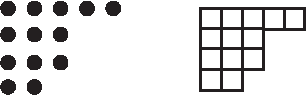
\includegraphics[width=0.33\linewidth]{images/FerrersYoung}
\caption{The Ferrers and Young diagrams of the partition (5,3,3,2)\label{FerrersYoung}}
\end{figure}
\begin{activity}[]\label{activity-139}
Draw the Young diagram of the partition (4,4,3,1,1). Describe the geometric relationship between the Young diagram of (5,3,3,2) and the Young diagram of (4,4,3,1,1).%
\par\medskip\noindent%
\textbf{Solution.}\quad \leavevmode%
\begin{figure}
\centering
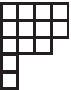
\includegraphics[width=0.33\linewidth]{images/Young44311}
\caption{Forming the conjugate of a Young diagram\label{Young44311}}
\end{figure}
We get the Young diagram of \((5,3,3,2)\) by flipping the Young diagram of \((4,4,3,1,1)\) around a line that includes the diagonal of the upper left box; if we think of the top left corner of the diagram as being at the origin, we flip around the line \(y=-x\).%
\end{activity}
\begin{activity}[]\label{activity-140}
The partition \((\lambda_1,\lambda_2,\ldots, \lambda_n)\) is called the \terminology{conjugate}\index{conjugate of an integer partition}\index{partition of an integer!conjugate of} of the partition \((\gamma_1,\gamma_2,\ldots, \gamma_m)\) if we obtain the Young diagram of one from the Young diagram of the other by flipping one around the line with slope -1 that extends the diagonal of the top left square. See \hyperref[conjugateYoung]{Figure~\ref{conjugateYoung}} for an example.%
\begin{figure}
\centering
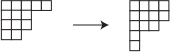
\includegraphics[width=0.5\linewidth]{images/conjugateYoung}
\caption{The Ferrers diagram the partition (5,3,3,2) and its conjugate.\label{conjugateYoung}}
\end{figure}
What is the conjugate of (4,4,3,1,1)? How is the largest part of a partition related to the number of parts of its conjugate? What does this tell you about the number of partitions of a positive integer \(k\) with largest part \(m\)?%
\par\medskip\noindent%
\textbf{Solution.}\quad \((5,3,3,2)\). The largest part of a partition equals the number of parts of its conjugate. The number of partitions of \(k\) with largest part \(m\) equals the number of partitions of \(k\) with \(m\) parts.%
\end{activity}
\begin{activity}[]\label{activity-141}
~\par
\begin{enumerate}[label=(\alph*)]
 \item A partition is called \emph{self-conjugate}\index{self-conjugate partition}\index{partition of an integer!self conjugate} if it is equal to its conjugate. Find a relationship between the number of self-conjugate partitions of \(k\) and the number of partitions of \(k\) into distinct odd parts.%
\par\medskip\noindent%
\textbf{Solution.}\quad The number of self-conjugate partitons of \(k\) equals the number of partitions of \(k\) with distinct odd parts. Here is a geometric description of a bijection from self conjugate partitions of \(k\) to partitions into distinct odd parts.%
\begin{figure}
\centering
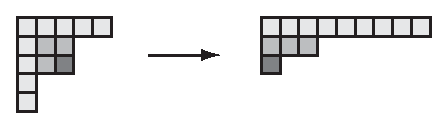
\includegraphics[width=0.33\linewidth]{images/selfconjugate}
\caption{Transforming a self-conjugate partition\label{selfconjugate-to-distinctodd}}
\end{figure}
Take the top row and left column of squares of the Young diagram, and make them into one row in a new diagram. (Only include the square that is in both the row and column once.) Now take the remaining squares in the next row and column and make a new row of the Young diagram of the second partition with them. Continue this process with succeeding rows and columns, not using any squares you have already used. Because the first partition is self conjugate, the diagram has the same number of rows as columns and row \(i\) and column \(i\) have the same length. Because row \(i\) and column \(i\) share one square, and we only use that square once when we create a new row, each row we create has odd length. Thus we get a partition with the same number of squares, so it is a partition of \(k\) and each part is odd. The parts are distinct because when we take off the squares of a row and column, we reduce the number of squares in each row and column that remains. Given a partition of \(k\) into distinct odd parts, we use the fact that each row has a unique middle element, and each is shorter than the one above (by at least two squares) to reverse the process. Thus we have a bijection.%

~\par
\item Explain the relationship between the number of partitions of \(k\) into even parts and the number of partitions of \(k\) into parts of even multiplicity, i.e. parts which are each used an even number of times as in (3,3,3,3,2,2,1,1).%
\par\medskip\noindent%
\textbf{Solution.}\quad The number of partitions of \(k\) into even parts equals the number of partitions of parts of even multiplicity, because if we take the Young diagram of a partition of \(k\) into even parts and conjugate it, the resulting diagram has columns of even length. Thus the difference in heights of two successive columns is an even number, but this difference is the multiplicity of one of the parts of the conjugate. Further the height of the last column of a partition is the multiplicity of the first part. Since the multiplicity of any part of a partition is either the difference in height of two successive columns of the Young diagram or the height of the last column, then each part of the conjugate has even multiplicity. This bijection can be reversed, because if all the differences in height of the columns are even and the height of the last column is even, then when we conjugate this partition, the last row will be an even length, and all differences in length of the rows will be even, so all the parts of the resulting partition will be even.%

\end{enumerate}
\end{activity}
\begin{activity}[]\label{rectanglecomplement}
~\par
\begin{enumerate}[label=(\alph*)]
 \item Show that the number of partitions of \(k\) into \(4\) parts equals the number of partitions of \(3k\) (or \(3k+4\) or \(3k-4\)) into \(4\) parts.%
\par\medskip\noindent%
\textbf{Solution.}\quad Think about putting the Young diagram of the partition into the upper left corner of a rectangle that is \(k\) units wide and four units high. Subdivide the rectangle into \(4k\) squares of unit area. The Young diagram covers \(k\) of these squares. The uncovered squares are in rows of length \(r_1\le r_2\le r_3\le r_4\). Thus if we list these lengths in the opposite order, we have a decreasing list representation of a partition of \(3k\). Even \(r_1\) will have to be positive, because the first part of the original partition will be at most \(k-3\). To get partitions of \(3k+4\), use a rectangle of width \(k+1\), and to get partitions of \(3k-4\), use a rectangle of width \(k-1\). Since the first row of the Young diagram has at most \(k-3\) squares, we will still have four nonzero parts in the partition that results.%

~\par
\item The idea of conjugation of a partition could be defined without the geometric interpretation of a Young diagram, but it would seem far less natural without the geometric interpretation. Another idea that seems much more natural in a geometric context is this. Suppose we have a partition of \(k\) into \(n\) parts with largest part \(m\). Then the Young diagram of the partition can fit into a rectangle that is \(m\) or more units wide (horizontally) and \(n\) or more units deep. Suppose we place the Young diagram of our partition in the top left-hand corner of an \(m'\) unit wide and \(n'\) unit deep rectangle with \(m'\ge m\) and \(n' \ge n\), as in \hyperref[complementpartition]{Figure~\ref{complementpartition}}.%
\begin{figure}
\centering
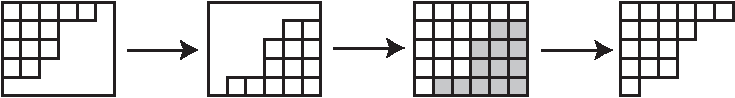
\includegraphics[width=0.33\linewidth]{images/complementpartition}
\caption{To complement the partition \((5,3,3,2)\) in a 6 by 5 rectangle: enclose it in the rectangle, rotate, and cut out the original Young diagram.\label{complementpartition}}
\end{figure}
Why can we interpret the part of the rectangle not occupied by our Young diagram, rotated in the plane, as the Young diagram of another partition? This is called the \terminology{complement}\index{complement of a partition} of our partition in the rectangle. What integer is being partitioned by the complement? What conditions on \(m'\) and \(n'\) guarantee that the complement has the same number of parts as the original one? What conditions on \(m'\) and \(n'\) guarantee that the complement has the same largest part as the original one? Is it possible for the complement to have both the same number of parts and the same largest part as the original one? If we complement a partition in an \(m'\) by \(n'\) box and then complement that partition in an \(m'\) by \(n'\) box again, do we get the same partition that we started with?%
\par\medskip\noindent%
\textbf{Solution.}\quad If we fill the rectangle with unit squares, those not in the Young diagram of the original partition \(\lambda\) will fall into rows.  The lengths of the rows are nonnegative, and are nondecreasing as we move down. Therefore, after we rotate through 180 degrees, these same rows will be listed in the opposite order, lined up along the left sides, and will have nonincreasing length. Thus they will be the Young diagram of a partition. The integer being partitioned will be \(m'n'-k\). If \(m'>m\) and \(n'=n\). the two partitions will have the same number of parts, because we will have a nonzero number of empty squares at the end of each row of the Young diagram of \(\lambda\). If \(m'=m\) and \(n'-n\) is the multiplicity of the largest part of \(\lambda\), they will have the same number of parts. Otherwise, their numbers of parts will differ. If \(n'>n\) and \(m=m'\), then the two partitions will have the same largest part. If \(n'=n\) and \(m'-m\) is the smallest part of \(\lambda\), then they will have the same largest part. Otherwise, their largest parts will differ. Thus for the two partitions to have the same number of parts, either \(m'=m\) or \(n'=n\). If \(m'=m\) and they have the same largest part, then \(n'>n\). But this is consistent with \(n'-n\) being the multiplicity of the largest part of \(\lambda\). Thus they can have the same number of parts and the same largest part if \(m'=m\) and \(n'-n\) is the multiplicity of the largest part of \(\lambda\), or similarly if \(n=n'\) and \(m'-m\) is the smallest part of \(\lambda\).%

\end{enumerate}
\end{activity}
\begin{activity}[]\label{activity-143}
~\par
\begin{enumerate}[label=(\alph*)]
 \item Suppose we take a partition of \(k\) into \(n\) parts with largest part \(m\), complement it in the smallest rectangle it will fit into, complement the result in the smallest rectangle it will fit into, and continue the process until we get the partition 1 of one into one part.  What can you say about the partition with which we started?%
\par\medskip\noindent%
\textbf{Solution.}\quad Let us call the process of enclosing \(\lambda\) in the smallest rectangle possible and then forming the complement in that rectangle \terminology{encomplementation} (This is short for \emph{en}\/closure and \emph{complementation} and is not a standard term\textemdash{}there is no standard term for this operation.) and call the result of it the \terminology{encomplement}\index{encomplement of a partition} of \(\lambda\).  The result of two encomplementations on the Young diagram of a partition is to remove all rows of maximum length and all columns of maximum length from the Young diagram. Thus the description of the result of an even number \(2j\) of encomplementations is straightforward; we remove all the rows of the \(j\) largest distinct lengths and all columns of the \(j\) largest distinct lengths. So if an even number of encomplementations brings us to a partition with one block of size one, we should be able to describe the original partition fairly easily. To deal with the result of an odd number of encomplementations, we ask what happens if we encomplement just once.  If the complement of \(\lambda\) in the smallest rectangle in which if fits has one square, then \(\lambda =\lambda_1^{n_1}\lambda_1-1\). Thus we are asking for the partitions which, after an even number of encomplementations, give us either the partition with one block or a partition of the form \(\lambda_1^{n_1}(\lambda_1-1)\). First we ask what kind of partition results in the second one after two encomplementations. If we get \(\lambda_1^{n_1}(\lambda_1-1)\) from two encomplementations, the partition we started with had the form%
\begin{equation*}
\lambda_0^{n_0}(\lambda_1+\lambda_{2})^{n_1}(\lambda_1+
\lambda_2-1)\lambda_2^{n_2}.
\end{equation*}
%
\par
If we get \(\lambda_1^{n_1}(\lambda_1-1)\) from four encomplementations, then we started with a partition of the form%
\begin{equation*}
\lambda_{-1}^{n_{-1}}(\lambda_0+\lambda_{3})^{n_0}(\lambda_1+
\lambda_2 +
\lambda_{3})^{n_1}(\lambda_1+\lambda_2 +\lambda_3-1)(\lambda_2+
\lambda_{3})^{n_3}
\lambda_3^{n_3}.
\end{equation*}
%
\par
From this pattern we see that a partition that results in \(\lambda_1^{n_1}(\lambda_1-1)\) after \(2j\) encomplementations has the form%
\begin{equation}
\lambda_{1-j}^{n_{1-j}}\lambda_{2-j}^{n_{2-j}}\cdots
\lambda_0^{n_0}
{\lambda'_1}^{n_1}
(\lambda'_1-1)\lambda_2^{n_2}\cdots
\lambda_{j+1}^{n_{j+1}},\label{form1}
\end{equation}
where \(\lambda_i>\lambda_{i+1}\) and \(\lambda_0>\lambda'_1>\lambda_2+1\).%
\par
On the other hand, a partition \(\lambda\) that results in \(1\) after two encomplementations has the form \(\lambda_0^{n_0}(\lambda_1+1)\lambda_1^{n_1}\), and so a partition that results in 1 after \(j\) encomplementations is of the form%
\begin{equation}
\lambda_{1-j}^{n_{1-j}}\lambda_{2-j}^{n_{2-j}}\cdots
\lambda_0^{n_0}(\lambda_1+1)\lambda_1^{n_1}\lambda_2^{n_2}\cdots
\lambda_j^{n_j},\label{form2}
\end{equation}
where \(\lambda_i>\lambda_{i+1}\) and \(\lambda_0>\lambda_1+1\). Thus a partition results in a single part of size 1 after some number of encomplementations if and only if it has the form of \hyperref[form1]{Equation~(\ref{form1})} or \hyperref[form2]{Equation~(\ref{form2})}.%

~\par
\item Show that \(P(k,n)\) is at least \({1\over n!}\binom{k-1}{n-1}\).%
\par\medskip\noindent%
\textbf{Solution.}\quad The number of compositions of \(k\) into \(n\) parts is \(\binom{k-1}{n-1}\). We can divide the compositions into blocks, where two compositions are in the same block if and only if one is a rearrangement of the other. Then the blocks correspond bijectively to partitions of \(k\) into \(n\) parts. However we cannot compute the number of blocks by dividing by the number of compositions per block since the number of compositions per block ranges from \(1\) to \(n!\).  But then if we divide the number of compositions by \(n!\) we will get a number less than the number of blocks because \(n!\) times the number of blocks would be, by the sum principle, greater than the number of partitions.%

\end{enumerate}
\end{activity}
With the binomial coefficients, with Stirling numbers of the second kind, and with the Lah numbers, we were able to find a recurrence by asking what happens to our subset, partition, or broken permutation of a set \(S\) of numbers if we remove the largest element of \(S\). Thus it is natural to look for a recurrence to count the number of partitions of \(k\) into \(n\) parts by doing something similar. Unfortunately, since we are counting distributions in which all the objects are identical, there is no way for us to identify a largest element. However if we think geometrically, we can ask what we could remove from a Young diagram to get a Young diagram. Two natural ways to get a partition of a smaller integer from a partition of \(n\) would be to remove the top row of the Young diagram of the partition and to remove the left column of the Young diagram of the partition. These two operations correspond to removing the largest part from the partition and to subtracting 1 from each part of the partition respectively. Even though they are symmetric with respect to conjugation, they aren't symmetric with respect to the number of parts. Thus one might be much more useful than the other for finding a recurrence for the number of partitions of \(k\) into \(n\) parts.%
\begin{activity}[]\label{numberpartitionrecurrence}
In this problem we will study the two operations and see which one seems more useful for getting a recurrence for \(P(k,n)\).%
~\par
\begin{enumerate}[label=(\alph*)]
 \item How many parts does the remaining partition have when we remove the largest part (more precisely, we reduce its multiplicity by one) from a partition of \(k\) into \(n\) parts?  What can you say about the number of parts of the remaining partition if we remove one from each part?%
\par\medskip\noindent%
\textbf{Solution.}\quad Reducing the multiplicity of the largest part by one reduces the number of parts by one. Removing 1 from each part reduces the number of parts by the multiplicity of the smallest part, so it strictly reduces the number of parts, perhaps even to one.%

~\par
\item If the largest part of a partition is \(j\) and we remove it, what integer is being partitioned by the remaining parts of the partition? If we remove one from each part of a partition of \(k\) into \(n\) parts, what integer is being partitioned by the remaining parts?%
\par\medskip\noindent%
\textbf{Solution.}\quad If we remove the largest part, the integer being partitioned is \(k\) minus the largest part. Thus it is a number less than \(k\) and at least \(n-1\). If we remove one from each part of the partition, the integer being partitioned is \(k-n\).%

~\par
\item The last two questions are designed to get you thinking about how we can get a bijection between the set of partitions of \(k\) into \(n\) parts and some other set of partitions that are partitions of a smaller number.  These questions describe two different strategies for getting that set of partitions of a smaller number or of smaller numbers.  Each strategy leads to a bijection between partitions of \(k\) into \(n\) parts and a set of partitions of a smaller number or numbers.  For each strategy, use the answers to the last two questions to find and describe this set of partitions into a smaller number and a bijection between partitions of \(k\) into \(n\) parts and partitions of the smaller integer or integers into appropriate numbers of parts.%
\par\medskip\noindent%
\textbf{Solution.}\quad Removing the largest part of a partition of \(k\) into \(n\) parts gives us a bijection between partitions of \(k\) into \(n\) parts and and partitions of numbers \(k'\) between \(n-1\) and \(k-1\) into \(n-1\) parts of size at most \(k-k'\). (Removing the largest part gives us such a partition, and adjoining a part of size \(k-k'\) to such a partition gives us a partition of \(k\) with \(n\) parts.)%
\par
Removing one from each part of a partition of \(k\) into \(n\) parts gives us a bijection between partitions of \(k\) into \(n\) parts and and partitions \(k-n\) into \(n\) or fewer parts. (Removing one from each part of a partition of \(k\) into \(n\) parts gives us such a partition, and, given such a partition, we get a partition of \(k\) into \(n\) parts by adding one to each part and then creating enough parts of size 1 to have \(n\) parts.)%

~\par
\item Find a recurrence (which need not have just two terms on the right hand side) that describes how to compute \(P(k,n)\) in terms of the number of partitions of smaller integers into a smaller number of parts.%
\par\medskip\noindent%
\textbf{Hint.}\quad One of the two sets of partitions of smaller numbers from the previous part is more amenable to finding a recurrence than the other.%
\par\medskip\noindent%
\textbf{Solution.}\quad The second bijection is to the set of partitions of \(k-1\) into \(n\) or fewer parts, and this makes the second bijection sound easier to work with. We get \(P(k,n)=\sum_{i=1}^n P(k-n,i)\). The proof is the bijection we already described; in particular a partition of \(k-n\) into \(i\) parts corresponds to the partition of \(k\) we get by adding one to each of the \(i\) parts and then creating \(n-i\) parts of size one.%

~\par
\item What is \(P(k,1)\) for a positive integer \(k\)?%
\par\medskip\noindent%
\textbf{Solution.}\quad \(P(k,1)=1\).%

~\par
\item What is \(P(k,k)\) for a positive integer \(k\)?%
\par\medskip\noindent%
\textbf{Solution.}\quad \(P(k,k)=1\).%

~\par
\item Use your recurrence to compute a table with the values of \(P(k,n)\) for values of \(k\) between 1 and 7.%
\par\medskip\noindent%
\textbf{Solution.}\quad \begin{tabular}{llllllll}
\(k\backslash n\)&1&2&3&4&5&6&7\tabularnewline[0pt]
&&&&&&&\tabularnewline\hrulethin
1&1&0&0&0&0&0&0\tabularnewline[0pt]
2&1&1&0&0&0&0&0\tabularnewline[0pt]
3&1&1&1&0&0&0&0\tabularnewline[0pt]
4&1&2&1&1&0&0&0\tabularnewline[0pt]
5&1&2&2&1&1&0&0\tabularnewline[0pt]
6&1&3&3&2&1&1&0\tabularnewline[0pt]
7&1&3&4&3&2&1&1
\end{tabular}

~\par
\item What would you want to fill into row 0 and column 0 of your table in order to make it consistent with your recurrence.  What does this say \(P(0,0)\) should be?  We usually define a sum with no terms in it to be zero. Is that consistent with the way the recurrence says we should define \(P(0,0)\)?%
\par\medskip\noindent%
\textbf{Solution.}\quad We would want to have \(P(0,0)=1\) and \(P(k,0)=P(0,n)=0\) for positive integer \(k\) or \(n\). Since the sum of the empty multiset of positive integers is zero, this gives us one partition of the number zero, namely the empty multiset of positive integers.%

\end{enumerate}
\end{activity}
It is remarkable that there is no known formula for \(P(k,n)\), nor is there one for \(P(k)\). This section was are devoted to developing methods for computing values of \(P(n,k)\) and finding properties of \(P(n,k)\) that we can prove even without knowing a formula. Some future sections will attempt to develop other methods.%
\par
We have seen that the number of partitions of \(k\) into \(n\) parts is equal to the number of ways to distribute \(k\) identical objects to \(n\) recipients so that each receives at least one. If we relax the condition that each recipient receives at least one, then we see that the number of distributions of \(k\) identical objects to \(n\) recipients is \(\sum_{i=1}^n P(k,i)\) because if some recipients receive nothing, it does not matter which recipients these are. This completes rows 7 and 8 of our table of distribution problems. The completed table is shown in \hyperref[lastdistributiontable]{Table~\ref{lastdistributiontable}}. There are quite a few theorems that you have proved which are summarized by \hyperref[lastdistributiontable]{Table~\ref{lastdistributiontable}}.  It would be worthwhile to try to write them all down!%
\begin{table}
\centering
\begin{tabular}{lll}
&&\tabularnewline\hrulethin
The Twentyfold Way: A Table of Distribution Problems\tabularnewline[0pt]
&&\tabularnewline\hrulemedium
\(k\) objects and conditions&\(n\) recipients and mathematical model for distribution\tabularnewline[0pt]
on how they are received&Distinct&Identical\tabularnewline[0pt]
&&\tabularnewline\hrulemedium
1.  Distinct&\(n^k\)&\(\sum_{i=1}^kS(n,i)\)\tabularnewline[0pt]
no conditions&functions&set partitions (\(\le n\) parts)\tabularnewline[0pt]
&&\tabularnewline\hrulethin
2.  Distinct&\(n^{\underline{k}}\)&1 if \(k\le n\); 0 otherwise\tabularnewline[0pt]
Each gets at most one&\kern -2pt \(k\)-element permutations\kern -2 pt&\tabularnewline[0pt]
&&\tabularnewline\hrulethin
3.  Distinct&\(S(k,n)n!\)&\(S(k,n)\)\tabularnewline[0pt]
Each gets at least one&onto functions&set partitions (\(n\) parts)\tabularnewline[0pt]
&&\tabularnewline\hrulethin
4. Distinct&\(k!=n!\)&1 if \(k=n\); 0 otherwise\tabularnewline[0pt]
Each gets exactly one&permutations&\tabularnewline[0pt]
&&\tabularnewline\hrulethin
5.  Distinct, order matters&\((k+n-1)^{\underline{k}}\)&\(\sum_{i=1}^n L(k,i)\)\tabularnewline[0pt]
&ordered functions&\hglue -3 pt broken permutations (\(\le n\) parts)\kern -3 pt\tabularnewline[0pt]
&&\tabularnewline\hrulethin
6.  Distinct, order matters&\((k)^{\underline{n}}(k-1)^{\underline{k-n}}\)&\(L(k,n)=
\binom{ k}{n}(k-1)^{\underline{k-n}}\)\tabularnewline[0pt]
Each gets at least one&ordered onto functions&broken permutations (\(n\) parts)\tabularnewline[0pt]
&&\tabularnewline\hrulethin
7.  Identical&\(\binom{n+k-1}{k}\)&\(\sum_{i=1}^nP(k,i)\)\tabularnewline[0pt]
no conditions&multisets&number partitions (\(\le n\) parts)\tabularnewline[0pt]
&&\tabularnewline\hrulethin
8.  Identical&\(\binom{n}{k}\)&1 if \(k\le n\); 0 otherwise\tabularnewline[0pt]
Each gets at most one&subsets&\tabularnewline[0pt]
&&\tabularnewline\hrulethin
9.  Identical&\(\binom{k-1}{n-1}\)&\(P(k,n)\)\tabularnewline[0pt]
Each gets at least one&compositions (\(n\) parts)&number partitions (\(n\) parts)\tabularnewline[0pt]
&&\tabularnewline\hrulethin
10.  Identical&1 if \(k=n\); 0 otherwise&1 if \(k=n\); 0 otherwise\tabularnewline[0pt]
Each gets exactly one&&\tabularnewline[0pt]
&&\tabularnewline\hrulethin
\end{tabular}
\caption{The number of ways to distribute \(k\) objects to \(n\) recipients, with restrictions on how the objects are received\label{lastdistributiontable}}
\end{table}
\typeout{************************************************}
\typeout{Subsection  Partitions into distinct parts}
\typeout{************************************************}
\subsection[{Partitions into distinct parts}]{Partitions into distinct parts}\label{subsection-39}
Often \(Q(k,n)\) is used to denote the number of partitions of \(k\) into distinct parts, that is, parts that are different from each other.%
\begin{activity}[]\label{activity-145}
Show that%
\begin{equation*}
Q(k,n) \le {1\over n!}\binom{k-1}{n-1}.
\end{equation*}
%
\par\medskip\noindent%
\textbf{Solution.}\quad The number of compositions of \(k\) into \(n\) parts is \(\binom{k-1}{n-1}\). Thus the number of compositions of \(k\) into \(n\) distinct parts is less than \(\binom{k-1}{n-1}\). Divide the compositions of \(k\) into \(n\) distinct parts into blocks with two compositions in the same block if one is a rearrangement of the other. Because the parts are distinct, each block has \(n!\) members. Further, there is a bijection between the blocks of this partition and the partitions of \(k\) into \(n\) distinct parts. Since the number of compositions of \(k\) into \(n\) distinct parts is less than \(\binom{k-1}{n-1}\), the number of partitions of \(k\) into \(n\) distinct parts is less than \({1\over n!}  \binom{k-1}{n-1}\).%
\end{activity}
\begin{activity}[]\label{activity-146}
Show that the number of partitions of 7 into 3 parts equals the number of partitions of 10 into three distinct parts.%
\par\medskip\noindent%
\textbf{Solution.}\quad Given a partition \(\lambda\) of 7 in decreasing list form \(\lambda_1,\lambda_2,\lambda_3\), if we add 0 to \(\lambda_3\), \(1\) to \(\lambda_2\) and 2 to \(\lambda_1\) the resulting partition of 10 has distinct parts. If we take a partition \(\lambda'\) of 10 with distinct parts, then \(\lambda'_1\ge\lambda'_2+1\), \(\lambda'_1\ge\lambda'_2+2\), and \(\lambda'_2\ge \lambda'_3+1\). Therefore if we subtract 2 from \(\lambda'_1\) to get \(\lambda_1\), subtract 1 from \(\lambda'_2\) to get \(\lambda_2\) and let \(\lambda_3= \lambda'_3\), then \(\lambda_1,\lambda_2,\lambda_3\) is the decreasing list representation of a partition of \(10-3=7\). Thus there is a bijection between partitions of \(7\) into three parts and partitions of \(10\) into three distinct parts.%
\end{activity}
\begin{activity}[]\label{activity-147}
There is a relationship between \(P(k,n)\) and \(Q(m,n)\) for some other number \(m\). Find the number \(m\) that gives you the nicest possible relationship.%
\par\medskip\noindent%
\textbf{Solution.}\quad The number of partitions of \(k\) into \(n\) parts is equal to the number of partitions of \(k+\binom{n}{2}\) into n distinct parts.  The bijection from partitions of \(k\) with \(n\) parts to partitions of \(k+\binom{n}{2}\) with \(n\) distinct parts that proves this is the one that takes a partition \(\lambda_n\lambda_{n-1}\cdots\lambda_1\) of \(k\) with \(\lambda_i>\lambda_{i+1}\) and adds \(i-1\) to \(\lambda_i\) to get \(\lambda'_i\). Then \(\lambda'\) is a partition into distinct parts, and the number it partitions is \(k+1+2+\cdots+n-1=k+\binom{n}{2}\). The proof that it is a bijection is the fact that subtracting \(n-i\) from the \(i\)\/th part of a partition of \(k\) into distinct parts yields a partition of \(k\), because part \(i+j\) is at least \(j\) smaller than part \(i\).%
\end{activity}
\begin{activity}[]\label{activity-148}
Find a recurrence that expresses \(Q(k,n)\) as a sum of \(Q(k-n,m)\) for appropriate values of \(m\).%
\par\medskip\noindent%
\textbf{Solution.}\quad Suppose \(\lambda\) is a partition of \(k\) into \(n\) distinct parts. Either 1 is one of those parts or not. Thus if we subtract 1 from each part, we either get a partition of \(k-n\) into \(n-1\) parts or a partition of \(k-n\) into \(n\) parts. If \(\lambda\) and \(\lambda'\) are different partitions of \(k\) into \(n\) distinct parts, they go to different partitions. Each partition of \(k-n\) into \(n-1\) parts or \(n\) parts can be gotten in this way from a corresponding partition of \(k\) into \(n\) parts. Thus we have a bijective correspondence and \(Q(k,n)=Q(k-n,n-1) +Q(k-n,n)\).%
\end{activity}
\begin{activity}[]\label{activity-149}
Show that the number of partitions of \(k\) into distinct parts equals the number of partitions of \(k\) into odd parts.%
\par\medskip\noindent%
\textbf{Solution.}\quad We start by giving a function from the set of partitions of \(k\) to the set of partitions of \(k\) with (only) odd parts. Clearly such a function cannot be one to one. Then we show that when restricted to the partitions with distinct parts it is one-to-one and onto by constructing an inverse. Given a partition \(\lambda_1^{i_1}\lambda_2^{i_2}\cdots\lambda_n^{i_n}\), write \(\lambda_i=\gamma_i2^{k_i}\), where \(\gamma_i\) is odd. (Thus \(2^{k_i}\) is the highest power of 2 that is a factor of \(\lambda_i\), so it is 1 if \(\lambda_i\) is odd.). It is possible that \(\gamma_i=\gamma_j\), for example if \(\lambda_i=36\) and \(\lambda_j=18\), then \(\gamma_i=\gamma_j=9\). We construct a new partition \(\pi\) whose parts are the numbers \(\gamma_j\) as follows: Given an odd number \(p\), let the multiplicity \(m(p)\) of \(p\) in \(\pi\) be \(\sum_{j: \gamma_j=m} 2^{k_j}\). Thus \(\sum_{p: m(p)\not=0}m(p)p = k\). Therefore, \(\pi\) is a partition of \(k\) whose parts are all odd.%
\par
Now consider a partition \(\pi\) of \(k\) whose parts are all odd. Let \(\pi=\pi_1^{r_1}\pi_2^{r_2}\cdots \pi_t^{r_t}\), with \(\pi_i>\pi_{i+1}\). (In terms of the multiplicity function \(m\), \(m(\pi_i) =r_i\), and \(\sum_{i=1}^t r_i\pi_i = k\).) We are going to write the binary expansion of each \(r_i\) as \(r_i = \sum_{j= 0}^{\lfloor \log_2 r_i\rfloor} 2^{ja_{ij}}\), where \(a_{ij}\) is 1 if \(2^j\) appears in the binary expansion of \(r_i\), and 0 otherwise. All of the numbers \(\pi_i2^{ja_{ij}}\) are distinct, because a power of two times one odd number cannot equal a power of two times another odd number. The numbers \(\pi_i2^{ja_{ij}}\) add to \(k\), so they are the parts of a partition \(\pi'\) of \(k\) into distinct parts. When we apply the function constructed in the first part of the solution to \(\pi'\), we get \(\pi\), so the correspondence between \(\pi\) and \(\pi'\) is a bijection.%
\end{activity}
\begin{activity}[]\label{activity-150}
Euler showed that if \(k\not= {3j^2+j\over 2}\), then the number of partitions of \(k\) into an even number of distinct parts is the same as the number of partitions of \(k\) into an odd number of distinct parts. Prove this, and in the exceptional case find out how the two numbers relate to each other.%
\par\medskip\noindent%
\textbf{Solution.}\quad This solution is taken largely from the book \textsl{Introduction to Combinatorics} by Ioan Tomescu (published in London by Collet's in 1975). Tomescu calls a collection of rows in a Young diagram a ``trapezoid'' if each row contains one less cell than the row above and the number of cells in the rows above and below the trapezoid differ by two or more from the number of cells in rows of the trapezoid. Thus in (8,6,5,4,2,1) we have 3 trapezoids, the first row, the next three rows, and the last two. Since we are dealing with partitions with distinct parts, we don't have to worry about how two equal rows affect the definition of a trapezoid. We will describe a way to transform a partition with an even number of distinct parts into a partition with an odd number of distinct parts and vice versa.%
\par
First we describe a transformation on Young diagrams. Here is the first part of the description. Suppose the smallest part \(m\) of \(\lambda\) is less than or equal to the number \(j\) of rows in the top trapezoid. Suppose further that if we have only one trapezoid, then \(j>m\). Then we construct a partition with one less part by adding 1 to each of the \(m\) largest parts and discarding the part \(m\). We still have a diagram for a partition of the same integer, but now the parity of the number of parts has changed, and we \emph{may} have increased the number of trapezoids by 1. The smallest part will now be larger than the number (now \(m\)) of rows in the top trapezoid. (Notice that the construction would not work if we had only one trapezoid and \(j=m\) because we would first remove one row of the trapezoid and thus have no row to which to attach one of our squares.)%
\par
Here is the second part of the description of the transformation. Suppose now that \(m\) is larger than the number \(j\) of rows of the top trapezoid in the Young diagram. Suppose also that the Young diagram has at least two trapezoids or it has one trapezoid and \(j\ge m-2\). Take one square from each of the \(j\) rows of the top trapezoid (which is the whole diagram if there is only one trapezoid) and also add a row of \(j\) squares at the bottom of the diagram. (Since \(m>j\), this gives us a Young diagram of a partition of the same integer into distinct parts.) The parity of the number of rows has changed, and now the number of rows of the top trapezoid is at least as large as the smallest part of the partition. (Note, two previously distinct trapezoids may have joined together to form one on top.)  (Notice that if we have one trapezoid and \(j= m+1\), then the construction yields a partition with two equal parts, which is why we made the special assumption above.) Now let \(T\) be the transformation described by the two constructions above. Its domain is all Young diagrams except those with one trapezoid and \(m\le j\le m+1\). \(T^2\) is the identity, and so \(T\) is a bijection.  When restricted to partitions with an odd number of parts, \(T\) gives partitions with an even number of parts, so on its domain it gives a bijection between partitions with an even number of parts and partitions with an odd number of parts.%
\par
If \(m=j\) and the diagram has just one trapezoid, then the diagram has \(3j^2-j\over 2\) squares, and if \(m=j+1\) and the diagram has just one trapezoid, then the diagram has \(3j^2+j\over 2\) squares. Thus if \(k\ne {3j^2\pm j\over 2}\), the number of partitions of \(k\) into distinct even parts equals the number of partitions of \(k\) into distinct odd parts.%
\par
If \(k= {3j^2\pm j\over 2}\) and \(j\) is even, then there is one diagram of a partition of \(k\) that is not in the domain of the bijection and has an even number of rows, so in this case there will be one more partition with an even number of parts than with an odd number. If \(k= {3j^2\pm j\over 2}\) and \(j\) is odd, there is one diagram with an odd number of rows not in the domain and so in this case there is one more partition with an odd number of parts than with an even number. This completes the exceptional cases of the problem.%
\end{activity}
\typeout{************************************************}
\typeout{Section 2.4 Supplementary Problems}
\typeout{************************************************}
\section[{Supplementary Problems}]{Supplementary Problems}\label{section-12}
\leavevmode%
\begin{enumerate}
\item\hypertarget{li-49}{}Answer each of the following questions with \(n^k\), \(k^n\), \(n!\), \(k!\), \(\binom{n}{k}\), \(\binom{k}{n}\), \(n^{\underline{k}}\), \(k^{\underline{n}}\), \(n^{\overline{k}}\), \(k^{\overline{n}}\), \(\binom{n+k-1}{k}\), \(\binom{n+k-1}{n}\), \(\binom{n-1}{k-1}\), \(\binom{k-1}{n-1}\), or ``none of the above". %
\begin{enumerate}
\item\hypertarget{li-50}{}In how many ways may we pass out \(k\) identical pieces of candy to \(n\) children? \(\binom{n+k-1}{k}\)%
%
\item\hypertarget{li-51}{}In how many ways may we pass out \(k\) distinct pieces of candy to \(n\) children? \(n^k\)%
%
\item\hypertarget{li-52}{}In how many ways may we pass out \(k\) identical pieces of candy to \(n\) children so that each gets at most one?  (Assume \(k\le n\).) \(\binom{n}{k}\).%
%
\item\hypertarget{li-53}{}In how many ways may we pass out \(k\) distinct pieces of candy to \(n\) children so that each gets at most one?  (Assume \(k\le n\).) \(n^{\underline{k}}\)%
%
\item\hypertarget{li-54}{}In how many ways may we pass out \(k\) distinct pieces of candy to \(n\) children so that each gets at least one?  (Assume \(k\ge n\).) None of the above.%
%
\item\hypertarget{li-55}{}In how many ways may we pass out \(k\) identical pieces of candy to \(n\) children so that each gets at least one?  (Assume \(k\ge n\).) \(\binom{k-1}{n-1}\)%
%
\end{enumerate}
%
\item\hypertarget{li-56}{}The neighborhood betterment committee has been given \(r\) trees to distribute to \(s\) families living along one side of a street. %
\begin{enumerate}
\item\hypertarget{li-57}{}In how many ways can they distribute all of them if the trees are distinct, there are more families than trees, and each family can get at most one? \(s^{\underline{r}}\)%
%
\item\hypertarget{li-58}{}In how many ways can they distribute all of them if the trees are distinct, any family can get any number, and a family may plant its trees where it chooses? \(s^r\)%
%
\item\hypertarget{li-59}{}In how many ways can they distribute all the trees if the trees are identical, there are no more trees than families,   and any family receives at most one? \(\binom{s}{r}\)%
%
\item\hypertarget{li-60}{}In how many ways can they distribute them if the trees are distinct, there are more trees than families, and each family receives at most one (so there could be some leftover trees)? \(\sum_{k=0}^s \binom{s}{k}r^{\underline{k}}\) or\(\sum_{k=0}^s s^{\underline{k}}\binom{r}{k}\)%
%
\item\hypertarget{multisetproblem}{}In how many ways can they distribute all the trees if they are identical and anyone may receive any number of trees? \(\binom{r+s-1}{r}\)%
%
\item\hypertarget{orderedfunctionproblem}{}In how many ways can all the trees be distributed and planted if the trees are distinct, any family can get any number, and a family must plant its trees in an evenly spaced row along the road? \(s^{\overline{r}}=(r+s-1)^{\underline{r}}\)%
%
\item\hypertarget{li-63}{}Answer the question in \hyperlink{orderedfunctionproblem}{Part~2.f} assuming that every family must get a tree. \(r!\binom{r-1}{s-1}\)%
%
\item\hypertarget{li-64}{}Answer the question in \hyperlink{multisetproblem}{Part~2.e} assuming that each family must get at least one tree. \(\binom{r-1}{s-1}\)%
%
\end{enumerate}
%
\item\hypertarget{li-65}{}In how many ways can \(n\) identical chemistry books, \(r\) identical mathematics books, \(s\) identical physics books, and \(t\) identical astronomy books be arranged on three bookshelves? (Assume there is no limit on the number of books per shelf.) \({(n+r+s+t+2)! \over n!r!s!t!2!}\)%
%
\item\hypertarget{li-66}{}(interesting) One formula for the Lah numbers is%
\begin{equation*}
L(k,n) = \binom{k}{n}(k-1)^{\underline{k-n}}
\end{equation*}
Find a proof that explains this product. First choose the \(n\) elements which will be the first member of the part they lie in. (This, in effect, labels the \(n\) parts.) Then assign the remaining \(k-n\) elements to their parts by making an ordered function of \(n-k\) objects to \(n\) recipients in \((n + (k-n) - 1)^{{k-n}} = (k-1)^{{k-n}}\) ways.%
%
\item\hypertarget{li-67}{}What is the number of partitions of \(n\) into two parts? \(n/2\) if \(n\) is even and \((n-1)/2\) if \(n\) is odd, equivalently, \(\lfloor n/2\rfloor\)%
%
\item\hypertarget{li-68}{}Show that the number of partitions of \(k\) into \(n\) parts of size at most \(m\) equals the number of partitions of \(mn-k\) into no more than \(n\) parts of size at most \(m-1\). If we take the complement of the Young diagram of a partition of \(k\) into \(n\) parts of size at most \(m\) in an rectangle with \(n\) rows and \(m\) columns, the number we partition will be \(mn-k\), and we will have no more than \(n\) parts, each of size at most \(m-1\). And if we take the complement of a partition of this second kind in the same rectangle, we will get a partition of the first kind.%
%
\item\hypertarget{li-69}{}Show that the number of partitions of \(k\) into parts of size at most \(m\) is equal to the number of partitions of of \(k+m\) into \(m\) parts. Given the first kind of partition, take the conjugate (giving a partition of \(k\) into at most \(m\) parts), add one to each part, and then add enough parts of size 1 to get a total of \(m\) parts. It is straightforward that this process can be reversed.%
%
\item\hypertarget{li-70}{}You can say something pretty specific about self-conjugate partitions of \(k\) into distinct parts.  Figure out what it is and prove it.  With that, you should be able to find a relationship between these partitions and partitions whose parts are consecutive integers, starting with 1.  What is that relationship? In a self-conjugate partition, the number of parts is the size of the largest part. If these parts are distinct, this means that each number between 1 and the largest part appears once as a part. That is, the parts are a list of consecutive integers, starting with 1.%
%
\item\hypertarget{li-71}{}What is \(s(k,1)\)? Since s\((k,1)\) is the coefficient of \(x^1\) in%
\begin{equation*}
x^{\underline{k}} = x(x-1)
(x-2)\cdot (x-(k-1)),
\end{equation*}
it is \((-1)^{k-1}(k-1)!\).%
%
\item\hypertarget{li-72}{}Show that the Stirling numbers of the second kind satisfy the recurrence%
\begin{equation*}
S(k,n) = \sum_{i=1}^kS(k-i,n-1)\binom{n-1}{i-1}.
\end{equation*}
A partition of \([k]\) into \(n\) blocks has a block containing \(k\). If this block has size \(i\), when you remove it, you get a partition of a set of size \(k-i\) into \(n-1\) blocks. The number of possible sets of size \(i\) containing \(k\) is \(\binom{k-1}{i-1}\), and \(i\) can be any number between 1 and \(k\). Each partition of \(k\) into \(n\) blocks may be constructed exactly once by first choosing the block containing \(k\) and then partitioning the remaining elements into \(n-1\) blocks. This proves the formula.%
%
\item\hypertarget{li-73}{}(interesting) Let \(c(k,n)\) be the number of ways for \(k\) children to hold hands to form \(n\) circles, where one child clasping his or her hands together and holding them out to form a circle is considered a circle.  Find a recurrence for \(c(k,n)\).  Is the family of numbers \(c(k,n)\) related to any of the other families of numbers we have studied? If so, how? The \(k\)th child is either in a circle by him/her self, and there are \(c(k-1,n-1)\) ways for this to happen, or is in a circle with some other children. In the second case child \(i\) can be to the immediate right of any of the other \(k-1\) children, so there are \((k-1)c(k-1,n)\) ways for this to happen. Thus \(c(k,n)=c(k-1,n-1)
+(k-1)c(k-1,n)\). This recurrence is almost the same as the recurrence for \(s(k,n)\), except it has a plus sign where the recurrence for the Stirling numbers of the first kind has a minus sign. Further \(c(k,1)=(k-1)!\) and \(c(k,k)=1\), which agrees, except for sign, with the Stirling numbers of the first kind. If we experiment with applying the recurrence, we see that whenever we use it to compute \(c(k,n)\), we get that \(c(k,n)=|s(k,n)|\). It is now straightforward to prove by induction that \(c(k,n)=|s(k,n)|\).%
%
\end{enumerate}
\typeout{************************************************}
\typeout{Chapter 3 Generating Functions}
\typeout{************************************************}
\chapter[{Generating Functions}]{Generating Functions}\label{ch_genfns}
\typeout{************************************************}
\typeout{Section 3.1 The Idea of Generating Functions}
\typeout{************************************************}
\section[{The Idea of Generating Functions}]{The Idea of Generating Functions}\label{sec_genfns-idea}
\typeout{************************************************}
\typeout{Introduction  }
\typeout{************************************************}
Suppose you are going to choose three pieces of fruit from among apples, pears and bananas for a snack.  We can symbolically represent all your choices as%
\begin{equation*}
\ap\ap\ap+\pe\pe\pe+\ba\ba\ba+\ap\ap\pe+\ap\ap\ba+\ap\pe\pe +\pe\pe\ba
+\ap\ba\ba+\pe\ba\ba+\ap\pe\ba.
\end{equation*}
%
\par
Here we are using a picture of a piece of fruit to stand for taking a piece of that fruit. Thus \(\ap\) stands for taking an apple, \(\ap\pe\) for taking an apple and a pear, and \(\ap\ap\) for taking two apples.  You can think of the plus sign as standing for the ``exclusive or,'' that is, \(\ap+\ba\) would stand for ``I take an apple or a banana but not both.'' To say ``I take both an apple and a banana,'' we would write \(\ap\ba\). We can extend the analogy to mathematical notation by condensing our statement that we take three pieces of fruit to%
\begin{equation*}
\ap^3+\pe^3+\ba^3+\ap^2\pe+\ap^2\ba +\ap\pe^2+\pe^2\ba+
\ap\ba^2+\pe\ba^2 +\ap\pe\ba.
\end{equation*}
%
\par
In this notation \(\ap^3\) stands for taking a multiset of three apples, while \(\ap^2\ba\) stands for taking a multiset of two apples and a banana, and so on. What our notation is really doing is giving us a convenient way to list all three element multisets chosen from the set \(\{\ap,\pe,\ba\}\).\footnote{This approach was inspired by George Pólya's paper ``Picture Writing,'' in the December, 1956 issue of the \emph{American Mathematical Monthly}, page 689. While we are taking a somewhat more formal approach than Pólya, it is still completely in the spirit of his work.\label{fn-9}}%
\par
Suppose now that we plan to choose between one and three apples, between one and two pears, and between one and two bananas. In a somewhat clumsy way we could describe our fruit selections as%
\begin{equation}
\ap\pe\ba+\ap^2\pe\ba+\cdots+\ap^2\pe^2\ba+\cdots +
\ap^2\pe^2\ba^2+\ap^3\pe\ba+
\cdots +\ap^3\pe^2\ba+\cdots +
\ap^3\pe^2\ba^2.\label{uptothreefruits}
\end{equation}
%
\begin{activity}[]\label{twopiecesoffruit}
Using an \(A\) in place of the picture of an apple, a \(P\) in place of the picture of a pear, and a \(B\) in place of the picture of a banana, write out the formula similar to \hyperref[uptothreefruits]{Formula~(\ref{uptothreefruits})} without any dots for left out terms. (You may use pictures instead of letters if you prefer, but it gets tedious quite quickly!) Now expand the product \((A+A^2+A^3)(P+P^2)(B+B^2)\) and compare the result with your formula.%
\par\medskip\noindent%
\textbf{Solution.}\quad \(APB+APB^2 +AP^2B+ AP^2B^2+ A^2PB+A^2PB^2+ A^2P^2B+ A^2P^2B^2+
A^3PB+A^3PB^2 +A^3P^2B+ A^3P^2B^2\)%
\begin{align*}
\amp \amp (A+A^2+A^3)(P+P^2)(B+B^2)\\
\amp =\amp APB+APB^2+AP^2B+AP^2B^2+A^2PB+A^2PB^2+A^2P^2B\\
\amp +\amp A^2P^2B^2+
A^3PB+A^3PB^2+A^3P^2B+A^3P^2B^2.
\end{align*}
%
\par
We get the same expression in both cases.%
\end{activity}
\begin{activity}[]\label{activity-152}
Substitute \(x\) for all of \(A\), \(P\) and \(B\) (or for the corresponding pictures) in the formula you got in \hyperref[twopiecesoffruit]{Problem~\ref{twopiecesoffruit}} and expand the result in powers of \(x\). Give an interpretation of the coefficient of \(x^n\).%
\par\medskip\noindent%
\textbf{Solution.}\quad \(x^3+3x^4+4x^5+3x^6+x^7\). There is one way to choose three pieces of fruit, there are three ways to choose four pieces, four ways to chose 5 pieces, three ways to choose 6 pieces , and there is one way to choose 7 pieces of fruit. The coefficient of \(x^n\) is the number of ways to choose \(n\) pieces of fruit.%
\end{activity}
If we were to expand the formula%
\begin{equation}
(\ap+\ap^2+\ap^3)(\pe+\pe^2)(\ba+\ba^2).\label{threefruitsagain}
\end{equation}
we would get \hyperref[uptothreefruits]{Formula~(\ref{uptothreefruits})}. Thus \hyperref[uptothreefruits]{formula~(\ref{uptothreefruits})} and \hyperref[threefruitsagain]{formula~(\ref{threefruitsagain})} each describe the number of multisets we can choose from the set \(\{\ap,\pe,\ba\}\) in which \(\apple\)~appears between 1 and three times and \(\pear\), and \(\banana\)~each appear once or twice. We interpret \hyperref[uptothreefruits]{Formula~(\ref{uptothreefruits})} as describing each individual multiset we can choose, and we interpret \hyperref[threefruitsagain]{Formula~(\ref{threefruitsagain})} as saying that we first decide how many apples to take, and then decide how many pears to take, and then decide how many bananas to take. At this stage it might seem a bit magical that doing ordinary algebra with the second formula yields the first, but in fact we could define addition and multiplication with these pictures more formally so we could explain in detail why things work out. However since the pictures are for motivation, and are actually difficult to write out on paper, it doesn't make much sense to work out these details. We will see an explanation in another context later on.%
\typeout{************************************************}
\typeout{Subsection  Picture functions}
\typeout{************************************************}
\subsection[{Picture functions}]{Picture functions}\label{picturefunction}
As you've seen, in our descriptions of ways of choosing fruits, we've treated the pictures of the fruit as if they are variables. You've also likely noticed that it is much easier to do algebraic manipulations with letters rather than pictures, simply because it is time consuming to draw the same picture over and over again, while we are used to writing letters quickly. In the theory of generating functions, we associate variables or polynomials or even power series with members of a set. There is no standard language describing how we associate variables with members of a set, so we shall invent some. By a \terminology{picture} of a member of a set we will mean a variable, or perhaps a product of powers of variables (or even a sum of products of powers of variables). A function that assigns a picture \(P(s)\) to each member \(s\) of a set \(S\) will be called a \terminology{picture function} . The \terminology{picture enumerator}\index{picture enumerator} for a picture function \(P\) defined on a set \(S\) will be%
\begin{equation*}
E_P(S) = \sum_{s: s\in S}  P(s).
\end{equation*}
%
\par
We choose this language because the picture enumerator lists, or enumerates, all the elements of \(S\) according to their pictures. Thus \hyperref[uptothreefruits]{Formula~(\ref{uptothreefruits})} is the picture enumerator the set of all multisets of fruit with between one and three apples, one and two pears, and one and two bananas.%
\begin{activity}[]\label{zerotothreeapples}
How would you write down a polynomial in the variable \(A\) that says you should take between zero and three apples?%
\par\medskip\noindent%
\textbf{Solution.}\quad \(A^0+A^1+A^2+A^3\).%
\end{activity}
\begin{activity}[]\label{zerotothreefruits}
How would you write down a picture enumerator that says we take between zero and three apples, between zero and three pears, and between zero and three bananas?%
\par\medskip\noindent%
\textbf{Solution.}\quad \((A^0+A^1+A^2+A^3)(P^0+P^1+P^2+P^3)(B^0+B^1+B^2+B^3).\)%
\end{activity}
\begin{activity}[]\label{activity-155}
(Used in \hyperref[groupsonsets]{Chapter~\ref{groupsonsets}}.) Notice that when we used \(A^2\) to stand for taking two apples, and \(P^3\) to stand for taking three pears, then we used the product \(A^2P^3\) to stand for taking two apples and three pears. Thus we have chosen the picture of the ordered pair (2 apples, 3 pears) to be the product of the pictures of a multiset of two apples and a multiset of three pears. Show that if \(S_1\) and \(S_2\) are sets with picture functions \(P_1\) and \(P_2\) defined on them, and if we define the picture of an ordered pair \((x_1,x_2)\in S_1\times S_2\) to be \(P((x_1,x_2))= P_1(x_1)P_2(x_2)\), then the picture enumerator of \(P\) on the set \(S_1\times S_2\) is \(E_{P_1}(S_1)E_{P_2}(S_2)\). We call this the \emph{product principle for picture enumerators}.\index{product principle!picture enumerators}\index{picture enumerators!product principle for}%
\par\medskip\noindent%
\textbf{Solution.}\quad %
\begin{align*}
E_P(S_1\times S_2)\amp =\amp \sum_{(x_1,x_2)\in S_1\times
S_2} P(x_1)P(x_2)\\
\amp =\amp 
\sum_{x_1:x_1\in S_1}\sum_{x_2:x_2\in S_2} P(x_1)P(x_2)\\
\amp =\amp \sum_{x_1\in S_1}P(x_1)\sum_{x_2\in S_2}P(x_2)\\
\amp =\amp \sum_{x_1\in S_1} P(x_1) E_{P_2}(S_2)\\
\amp =\amp \left(\sum_{x_1\in S_1} P(x_1)\right)E_{P_2}(S_2)\\
\amp =\amp E_{P_1}(S_1)E_{P_2}(S_2)
\end{align*}
%
\end{activity}
\typeout{************************************************}
\typeout{Subsection  Generating functions}
\typeout{************************************************}
\subsection[{Generating functions}]{Generating functions}\label{subsection-41}
\begin{activity}[]\label{activity-156}
Suppose you are going to choose a snack of between zero and three apples, between zero and three pears, and between zero and three bananas. Write down a polynomial in one variable \(x\) such that the coefficient of \(x^n\) is the number of ways to choose a snack with \(n\) pieces of fruit.%
\par\medskip\noindent%
\textbf{Hint.}\quad Substitute something for \(A\), \(P\) and \(B\) in your formula from \hyperref[zerotothreefruits]{Activity~\ref{zerotothreefruits}}.%
\par\medskip\noindent%
\textbf{Solution.}\quad \((1+x+x^2+x^3)^3\)%
\end{activity}
\begin{activity}[]\label{activity-157}
Suppose an apple costs 20 cents, a banana costs 25 cents, and a pear costs 30 cents. What should you substitute for \(A\), \(P\), and \(B\) in \hyperref[zerotothreefruits]{Problem~\ref{zerotothreefruits}} in order to get a polynomial in which the coefficient of \(x^n\) is the number of ways to choose a selection of fruit that costs \(n\) cents?%
\par\medskip\noindent%
\textbf{Solution.}\quad Substitute \(x^{20}\) for \(A\), \(x^{25}\) for \(B\) and \(x^{30}\) for \(P\).%
\end{activity}
\begin{activity}[]\label{activity-158}
Suppose an apple has 40 calories, a pear has 60 calories, and a banana has 80 calories. What should you substitute for \(A\), \(P\), and \(B\) in \hyperref[zerotothreefruits]{Problem~\ref{zerotothreefruits}} in order to get a polynomial in which the coefficient of \(x^n\) is the number of ways to choose a selection of fruit with a total of \(n\) calories?%
\par\medskip\noindent%
\textbf{Solution.}\quad Substitute \(x^{40}\) for \(A\), \(x^{60}\) for \(P\), and \(x^{80}\) for \(B\).%
\end{activity}
\begin{activity}[]\label{reprovingbinomialtheorem}
We are going to choose a subset of the set \([n]=\{1,2,\ldots, n\}\). Suppose we use \(x_1\) to be the picture of choosing 1 to be in our subset. What is the picture enumerator for either choosing 1 or not choosing 1? Suppose that for each \(i\) between 1 and \(n\), we use \(x_i\) to be the picture of choosing \(i\) to be in our subset. What is the picture enumerator for either choosing \(i\) or not choosing \(i\) to be in our subset? What is the picture enumerator for all possible choices of subsets of \([n]\)? What should we substitute for \(x_i\) in order to get a polynomial in \(x\) such that the coefficient of \(x^k\) is the number of ways to choose a \(k\)-element subset of \(n\)? What theorem have we just reproved (a special case of)?%
\par\medskip\noindent%
\textbf{Solution.}\quad The picture enumerator for choosing \(1\) or not choosing 1 is \(x_1+1\). The picture enumerator for choosing or not choosing \(i\) is \(x_i+1\).  The picture enumerator for choosing all possible subsets of \([n]\) is \((x_1+1)(x_2+1)\cdots(x_n+1).\) We should substitute \(x\) for \(x_i\), thus getting \((1+x)^n\). Since the number of ways to choose an \(n\)-element subset is \(\binom{n}{k}\), we have just proved the version of the binomial theorem that says%
\begin{equation*}
(x+1)^n=\sum_{i=0}^n \binom{n}{i}x^i.
\end{equation*}
%
\end{activity}
In \hyperref[reprovingbinomialtheorem]{Problem~\ref{reprovingbinomialtheorem}} we see that we can think of the process of expanding the polynomial \((1+x)^n\) as a way of ``generating'' the binomial coefficients \(\binom{n}{k}\) as the coefficients of \(x^k\) in the expansion of \((1+x)^n\). For this reason, we say that \((1+x)^n\) is the ``generating function'' for the binomial coefficients \(\binom{n}{k}\). More generally, the \terminology{generating function} for a sequence \(a_i\), defined for \(i\) with \(0\le i\le n\) is the expression \(\sum_{i=0}^n a_ix^i\), and the \terminology{generating function}\index{generating function} for the sequence \(a_i\) with \(i\ge 0\) is the expression \(\sum_{i=0}^\infty a_ix^i\). This last expression is an example of a power series. In calculus it is important to think about whether a power series converges in order to determine whether or not it represents a function. In a nice twist of language, even though we use the phrase generating function as the name of a power series in combinatorics, we don't require the power series to actually represent a function in the usual sense, and so we don't have to worry about convergence.\footnote{In the evolution of our current mathematical terminology, the word function evolved through several meanings, starting with very imprecise meanings and ending with our current rather precise meaning.  The terminology ``generating function'' may be thought of as an example of one of the earlier usages of the term function.\label{fn-10}} Instead we think of a power series as a convenient way of representing the terms of a sequence of numbers of interest to us. The only justification for saying that such a representation is convenient is because of the way algebraic properties of power series capture some of the important properties of some sequences that are of combinatorial importance. The remainder of this chapter is devoted to giving examples of how the algebra of power series reflects combinatorial ideas.%
\par
Because we choose to think of power series as strings of symbols that we manipulate by using the ordinary rules of algebra and we choose to ignore issues of convergence, we have to avoid manipulating power series in a way that would require us to add infinitely many real numbers. For example, we cannot make the substitution of \(y+1\) for \(x\) in the power series \(\sum_{i=0}^\infty x^i\), because in order to interpret \(\sum_{i=0}^\infty (y+1)^i\) as a power series we would have to apply the binomial theorem to each of the \((y+1)^i\) terms, and then collect like terms, giving us infinitely many ones added together as the coefficient of \(y^0\), and in fact infinitely many numbers added together for the coefficient of any~\(y^i\). (On the other hand, it would be fine to substitute \(y+y^2\) for \(x\). Can you see why?)%
\typeout{************************************************}
\typeout{Subsection  Power series}
\typeout{************************************************}
\subsection[{Power series}]{Power series}\label{subsection-42}
For now, most of our uses of power series will involve just simple algebra. Since we use power series in a different way in combinatorics than we do in calculus, we should review a bit of the algebra of power series.%
\begin{activity}[]\label{coeffinproduct}
In the polynomial \((a_0 +a_1x+a_2x^2)(b_0+b_1x+b_2x^2+b_3x^3)\), what is the coefficient of \(x^2\)? What is the coefficient of \(x^4\)?%
\par\medskip\noindent%
\textbf{Solution.}\quad \(a_0b^2+a_1b_1+a_2b_0\) is the coefficient of \(x^2\). \(a_1b_3+a_2b_2\) is the coefficient of \(x^4\).%
\end{activity}
\begin{activity}[]\label{coeffinproduct1}
In \hyperref[coeffinproduct]{Problem~\ref{coeffinproduct}} why is there a \(b_0\) and a \(b_1\) in your expression for the coefficient of \(x^2\) but there is not a \(b_0\) or a \(b_1\) in your expression for the coefficient of \(x^4\)? What is the coefficient of \(x^4\) in%
\begin{equation*}
(a_0+a_1x+a_2x^2+a_3x^3+a_4x^4)(b_0+b_1x+b_2x^2
+b_3x^3+b_4x^4)?
\end{equation*}
%
\par
Express this coefficient in the form%
\begin{equation*}
\sum_{i=0}^4 \mbox{ something} ,
\end{equation*}
where the something is an expression you need to figure out. Now suppose that \(a_3=0\), \(a_4=0\) and \(b_4=0\). To what is your expression equal after you substitute these values? In particular, what does this have to do with \hyperref[coeffinproduct]{Problem~\ref{coeffinproduct}}?%
\par\medskip\noindent%
\textbf{Solution.}\quad There is a \(b_0\) because it can be paired with an \(a_2\) to give the term \(a_2b_0x^4\). Similarly there is a \(b_1\) because it can be paired with \(a_1\) for the same purpose. However there is no \(a_i\) that we can pair with \(b_0\) to get a coefficient of \(x^4\) and no \(a_i\) that we can pair with \(b_3\) to get a coefficient of \(x^4\).%
\par
The coefficient of \(x^4\) in%
\begin{equation*}
(a_0+a_1x+a_2x^2+a_3x^3+a_4x^4)(b_0+b_1x+b_2x^2
+b_3x^3+b_4x^4)
\end{equation*}
is \(\sum_{i=0}^4 a_ib_{4-i}\). If we substitute \(a_3=0\), \(a_4=0\), and \(b_4 =0\), we get the coefficient of \(x^4\) in \((a_0
+a_1x+a_2x^2)(b_0+b_1x+b_2x^2+b_3x^3)\). This exemplifies the idea that we can get a uniform formula for the coefficient of \(x^i\) (namely, sum all \(a_jb_{i-j}\) from \(j=0\) to \(i\)) in a product of two polynomials if we are willing to say that the coefficient of a power of \(x\) that does not appear in a polynomial is 0.%
\end{activity}
\begin{activity}[]\label{activity-162}
The point of the \hyperref[coeffinproduct]{Problems~\ref{coeffinproduct}} and \hyperref[coeffinproduct1]{Activity~\ref{coeffinproduct1}} is that so long as we are willing to assume \(a_i=0\) for \(i>n\) and \(b_j =0\) for \(j>m\), then there is a very nice formula for the coefficient of \(x^k\) in the product%
\begin{equation*}
\left(\sum_{i=0}^n a_ix^i\right)\left(\sum_{j=0}^m b_jx^j\right).
\end{equation*}
%
\par
Write down this formula explicitly.%
\par\medskip\noindent%
\textbf{Solution.}\quad \(\sum_{i=0}^k a_ib_{k-i}\).%
\end{activity}
\begin{activity}[]\label{coeffinpowerseries}
Assuming that the rules you use to do arithmetic with polynomials apply to power series, write down a formula for the coefficient of \(x^k\) in the product%
\begin{equation*}
\left(\sum_{i=0}^\infty a_ix^i\right)\left(\sum_{j=0}^\infty
b_jx^j\right).
\end{equation*}
%
\par\medskip\noindent%
\textbf{Solution.}\quad \(\sum_{i=0}^k a_ib_{k-i}\).%
\end{activity}
We use the expression you obtained in \hyperref[coeffinpowerseries]{Problem~\ref{coeffinpowerseries}} to \emph{define} the product of power series. That is, we define the product%
\begin{equation*}
\left(\sum_{i=0}^\infty a_ix^i\right)\left(\sum_{j=0}^\infty
b_jx^j\right)
\end{equation*}
to be the power series \(\sum_{k=0}^\infty c_k x^k\), where \(c_k\) is the expression you found in \hyperref[coeffinpowerseries]{Problem~\ref{coeffinpowerseries}}. Since you derived this expression by using the usual rules of algebra for polynomials, it should not be surprising that the product of power series satisfies these rules.\footnote{Technically we should explicitly state these rules and prove that they are all valid for power series multiplication, but it seems like overkill at this point to do so!\label{fn-11}}%
\typeout{************************************************}
\typeout{Subsection  Product principle for generating functions}
\typeout{************************************************}
\subsection[{Product principle for generating functions}]{Product principle for generating functions}\label{subsection-43}
Each time that we converted a picture function to a generating function by substituting \(x\) or some power of \(x\) for each picture, the coefficient of \(x\) had a meaning that was significant to us. For example, with the picture enumerator for selecting between zero and three each of apples, pears, and bananas, when we substituted \(x\) for each of our pictures, the exponent \(i\) in the power \(x^i\) is the number of pieces of fruit in the fruit selection that led us to \(x^i\). After we simplify our product by collecting together all like powers of \(x\), the coefficient of \(x^i\) is the number of fruit selections that use \(i\) pieces of fruit. In the same way, if we substitute \(x^c\) for a picture, where \(c\) is the number of calories in that particular kind of fruit, then the \(i\) in an \(x^i\) term in our generating function stands for the number of calories in a fruit selection that gave rise to \(x^i\), and the coefficient of \(x^i\) in our generating function is the number of fruit selections with \(i\) calories.  The product principle of picture enumerators translates directly into a product principle for generating functions.%
\begin{activity}[]\label{ProductPrincipleOGF}
Suppose that we have two sets \(S_1\) and \(S_2\). Let \(v_1\) (\(v\) stands for value) be a function from \(S_1\) to the nonnegative integers and let \(v_2\) be a function from \(S_2\) to the nonnegative integers.  Define a new function \(v\) on the set \(S_1 \times S_2\) by \(v(x_1,x_2) = v_1(x_1) +v_2(x_2)\). Suppose further that \(\sum_{i=0}^\infty a_ix^i\) is the generating function for the number of elements \(x_1\) of \(S_1\) of value \(i\), that is with \(v_1(x_1)=i\). Suppose also that \(\sum_{j=0}^\infty b_j x^j\) is the generating function for the number of elements of \(x_2\) of \(S_2\) of value \(j\), that is with \(v_2(x_2) = j\).  Prove that the coefficient of \(x^k\) in%
\begin{equation*}
\left(\sum_{i=0}^\infty a_ix^i\right)\left(\sum_{j=0}^\infty
b_jx^j\right)
\end{equation*}
is the number of ordered pairs \((x_1,x_2)\) in \(S_1\times S_2\) with total value \(k\), that is with \(v_1(x_1) +v_2(x_2) =k\). This is called the \terminology{product principle for generating functions}.\index{product principle for generating functions}\index{generating function!product principle for}%
\par\medskip\noindent%
\textbf{Solution.}\quad The generating function for ordered pairs of total value \(k\) will have the number of ordered pairs of total value \(k\) as the coefficient of \(x^k\). But we get a total value \(k\) by taking something of value \(i\) in \(S_1\) and something of value \(k-i\) in \(j\). And since values cannot be negative, the only \(i\)s available to us are the ones between \(0\) and \(k\). By the product principle for pairs, the number of ordered pairs \((x,y)\) with \(v_1(x)=i\) and \(v_2(y)=k-i\) is \(a_ib_{k-i}\). To get the number of pairs of total value \(k\), we have to sum over all possible pairs \((i,k-i)\) of values, that is, we have to take the sum \(\sum_{i=0}^k a_ib_{k-i}\). And this is the coefficient of \(x^k\) in the product%
\begin{equation*}
\left(\sum_{i=0}^\infty a_ix^i\right)\left(\sum_{j=0}^\infty
b_jx^j\right).
\end{equation*}
%
\par
This proves the product principle for generating functions.%
\end{activity}
\begin{activity}[]\label{activity-165}
Let \(i\) denote an integer between 1 and \(n\).%
~\par
\begin{enumerate}[label=(\alph*)]
 \item What is the generating function for the number of subsets of \(\{i\}\) of each possible size? (Notice that the only subsets of \(\{i\}\) are \(\emptyset\) and \(\{i\}\).)%
\par\medskip\noindent%
\textbf{Solution.}\quad \(1+x\).%

~\par
\item Use the product principle for generating functions to prove the binomial theorem.%
\par\medskip\noindent%
\textbf{Solution.}\quad The generating function for number of \(n\)-tuples of 0s and 1s with \(k\) ones is, by the product principle for generating functions (extended to \(n\) factors) \((1+x)^n\). However the number of \(n\)-tuples of 0s and 1s with \(k\) ones is the number of \(k\)-element subsets of an \(n\)-element set. Therefore \((1+x)^n =\sum_{i=0}^n \binom{n}{i}x^i\). To get the \((x+y)^n\) form of the binomial theorem, note that \(x+y = y(1+{x\over y})\), so that%
\begin{align*}
(x+y)^n \amp =\amp  y^n\left({x\over y}+1\right)^n\\
\amp =\amp y^n\sum_{i=0}^n \binom{n}{i}{x^i\over y^i}\\
\amp =\amp  \sum_{i=0}^n\binom{n}{i}x^iy^{n-i}.
\end{align*}
%

\end{enumerate}
\end{activity}
\typeout{************************************************}
\typeout{Subsection  The extended binomial theorem and multisets}
\typeout{************************************************}
\subsection[{The extended binomial theorem and multisets}]{The extended binomial theorem and multisets}\label{subsection-44}
\begin{activity}[]\label{activity-166}
Suppose once again that \(i\) is an integer between 1 and \(n\).%
~\par
\begin{enumerate}[label=(\alph*)]
 \item What is the generating function in which the coefficient of \(x^k\) is the number of multisets of size \(k\) chosen from \(\{i\}\)?  This series is an example of what is called an \terminology{infinite geometric series}.\index{geometric series}\index{series!geometric}%
\par\medskip\noindent%
\textbf{Solution.}\quad \(1+x+x^2+\cdots+x^i+\cdots=\sum_{i=0}^\infty x^i\).%

~\par
\item Express the generating function in which the coefficient of \(x^k\) is the number of multisets chosen from \([n]\) as a power of a power series.  What does \hyperref[multiset]{Problem~\ref{multiset}} (in which your answer could be expressed as a binomial coefficient) tell you about what this generating function equals?%
\par\medskip\noindent%
\textbf{Solution.}\quad The generating function is \(\left(\sum_{i=0}^\infty x^i\right)^n\).  \hyperref[multiset]{Problem~\ref{multiset}} tells us that this equals \(\sum_{i=0}^\infty\binom{n+i-1}{i}x^i\).%

\end{enumerate}
\end{activity}
\begin{activity}[]\label{activity-167}
What is the product \((1-x)\sum_{k=0}^n x^k\)? What is the product%
\begin{equation*}
(1-x)\sum_{k=0}^\infty x^k?
\end{equation*}
%
\par\medskip\noindent%
\textbf{Solution.}\quad %
\begin{equation*}
(1-x)\sum_{k=0}^n x^k=1-x+x-x^2+\cdots+x^{n-1}-x^n+x^n-x^{n+1} =
1-x^{n+1}.
\end{equation*}
%
\begin{equation*}
(1-x)\sum_{k=0}^\infty x^k=\sum_{i=0}^\infty x^i-\sum_{i=0}^\infty
x^{i+1}=\sum_{i=0}^\infty x^i-\sum_{i=1}^\infty x^i = 1.
\end{equation*}
%
\end{activity}
\begin{activity}[]\label{activity-168}
Express the generating function for the number of multisets of size \(k\) chosen from \([n]\) (where \(n\) is fixed but \(k\) can be any nonnegative integer) as a 1 over something relatively simple.%
\par\medskip\noindent%
\textbf{Solution.}\quad Since \((1-x)\sum_{k=0}^\infty x^k=1\), we have that%
\begin{equation*}
\sum_{k=0}^\infty x^k={1\over 1-x}.
\end{equation*}
%
\par
Therefore \(\left(\sum_{k=0}^\infty
x^k\right)^n= {1\over(1-x)^n}\) is the generating function for multisets of size \(k\) chosen from an \(n\) element set.%
\end{activity}
\begin{activity}[]\label{negnchoosek}
Find a formula for \((1+x)^{-n}\) as a power series whose coefficients involve binomial coefficients. What does this formula tell you about how we should define \(\binom{-n}{k}\) when \(n\) is positive?%
\par\medskip\noindent%
\textbf{Solution.}\quad %
\begin{equation*}
(1+x)^{-n}=(1-(-x))^{-n}=\sum_{i=0}^\infty
\binom{n+i-1}{i}(-x)^i=\sum_{i=0}^\infty (-1)^i\binom{n+i-1}{i}x^i.
\end{equation*}
We want the coefficient of \(x^k\) in \((1+x)^{-n}\) to be \(\binom{-n}{k}\), so we want \(\binom{-n }{k}= (-1)^k\binom{n+k-1}{k}\).%
\end{activity}
\begin{activity}[]\label{activity-170}
If you define \(\binom{-n}{k}\) in the way you described in \hyperref[negnchoosek]{Problem~\ref{negnchoosek}}, you can write down a version of the binomial theorem for \((x+y)^n\) that is valid for both nonnegative and negative values of \(n\). Do so. This is called the \terminology{extended binomial theorem}\index{binomial theorem!extended}\index{extended binomial theorem}.%
\par\medskip\noindent%
\textbf{Solution.}\quad \((x+y)^n=\sum_{i=0}^\infty\binom{n}{i}x^i\). The proof consists of writing \((x+y)=y({x\over y}+1)\) and applying the \hyperref[negnchoosek]{Problem~\ref{negnchoosek}} when \(n\) is negative. When \(n\) is positive, we recall that \(\binom{n}{k}\) is zero when \(k>n\), so replacing the upper limit of \(n\) in the standard version of the binomial theorem by \(\infty\) doesn't change the value of the sum.%
\end{activity}
\begin{activity}[]\label{activity-171}
Write down the generating function for the number of ways to distribute identical pieces of candy to three children so that no child gets more than 4 pieces. Write this generating function as a quotient of polynomials. Using both the extended binomial theorem and the original binomial theorem, find out in how many ways we can pass out exactly ten pieces. Use one of our earlier counting techniques to verify your answer.%
\par\medskip\noindent%
\textbf{Solution.}\quad \((1+x+x^2+x^3+x^4)^3\). We can write%
\begin{align*}
\amp \amp (1+x+x^2+x^3+x^4)^3 \rangle =\rangle \left({1-x^5\over 1-x}\right)^3\\
\amp =\amp (1-x^5)^3(1-x)^{-3}\\
\amp =\amp (1-3x^5+3x^{10}-x^{15})\sum_{i=0}^\infty \binom{3+i-1}{i}x^i\\
\amp =\amp (1-3x^5+3x^{10}-x^{15})\sum_{i=0}^\infty \binom{2+i}{i}x^i
\end{align*}
%
\par
The coefficient of \(x^{10}\) is the number of ways to pass out ten pieces of candy, and is \(\binom{12}{10}-3\binom{7}{5} +3\binom{2}{0}\).  Thus the number of ways to pass out ten pieces of candy is \(66-3\cdot21+3=6\).)%
\par
A second solution technique that is appropriate is inclusion-exclusion counting. We let property \(i\) be that child \(i\) gets more than four pieces of fruit. The number of ways to pass out \(n\) pieces of fruit with a set \(J\) of size \(j\) properties is \(\binom{n-5j+3-1}{n-5j}=\binom{n-5j+2}{2}\). By \hyperref[incexempty]{Equation~(\ref{incexempty})} we have \(N_{\mbox{e} }(\emptyset) = \sum_{j=0}^3 (-1)^j\binom{3}{j}\binom{n-5j+2}{2}\). Using \(n=10\) gives us \(\binom{12}{2}-3\binom{7}{2} +3\binom{2}{2} =6.\) (You can either note that \(\binom{-3}{2}\) is 0 or note that with 10 pieces of candy, there is no way to pass out five pieces to each of three children. In this second case we would revise our statement about the number of ways to pass out \(n\) pieces of fruit to three children with the properties in \(J\) to note that it is zero if \(5j>n\), and otherwise is \(\binom{n-5j+2}{2}\).)%
\end{activity}
\begin{activity}[]\label{activity-172}
What is the generating function for the number of multisets chosen from an \(n\)-element set so that each element appears at least \(j\) times and less than \(m\) times. Write this generating function as a quotient of polynomials, then as a product of a polynomial and a power series.%
\par\medskip\noindent%
\textbf{Solution.}\quad %
\begin{align*}
(x^j+x^{j+1}+\cdots+x^{m-1})\amp =\amp x^j
\left(\sum_{i=0}^{m-j-1}x^i\right)^n\\
\amp =\amp 
\left(x^j{1-x^{m-j}\over 1-x}\right)^n\\
\amp =\amp \left({x^j-x^m\over1-x}\right)^n\\
\amp =\amp  (x^j-x^m)^n\sum_{i=0}^\infty \binom{n+i-1}{i}x^i.
\end{align*}
%
\end{activity}
\typeout{************************************************}
\typeout{Subsection  Generating functions for integer partitions}
\typeout{************************************************}
\subsection[{Generating functions for integer partitions}]{Generating functions for integer partitions}\label{subsection-45}
\begin{activity}[]\label{change-making}
If we have five identical pennies, five identical nickels, five identical dimes, and five identical quarters, give the picture enumerator for the combinations of coins we can form and convert it to a generating function for the number of ways to make \(k\) cents with the coins we have. Do the same thing assuming we have an unlimited supply of pennies, nickels, dimes, and quarters.%
\par\medskip\noindent%
\textbf{Solution.}\quad \((1+P+P^2+P^3+P^4+P^5)(1+N+N^2+N^3+N^4+N^5)(1+D+D^2+D^3+D^4+D^5)
(1+Q+Q^2+Q^3+Q^4+Q^5)\). Substituting \(x\) for \(P\), \(x^5\) for \(N\), \(x^{10}\) for \(D\) and \(x^{25}\) for \(Q\) gives us%
\begin{equation*}
\sum_{i=0}^5x^i\sum_{i=0}^5x^{5i}\sum_{i=0}^5 x^{10i} \sum_{i=0}^5
x^{25i}={1-x^6\over1-x}\cdot{1-x^{30}\over 1-x^5}\cdot{1-x^{60}\over
1-x^{10}}\cdot{1-x^{150}\over 1-x^{25}}.
\end{equation*}
%
\par
Although we could write this as a polynomial times a product of four power series, doing so would not significantly increase our understanding, though it would let us make some painful computations of the number of ways to make a certain number of cents. If we actually wanted such numbers we would be better off asking a computer algebra package to expand the product of the polynomials on the left. With unlimited supplies the generating function becomes%
\begin{equation*}
{1\over1-x}\cdot{1\over 1-x^5}\cdot{1\over 1-x^{10}}\cdot{1\over 1-x^{25}}.
\end{equation*}
%
\par
Again, we could write this as a product of power series, and that would allow us to painfully compute the number of ways to create a certain number of cents. If we actually wanted to know the number of ways to make up 200 cents, say, it would be more sensible to ask a computer algebra package to extract the coefficient of \(x^{200}\) in the product of the four quotients.%
\end{activity}
\begin{activity}[]\label{largestpartatmostm}
Recall that a partition of an integer \(k\) is a multiset of numbers that adds to \(k\). In \hyperref[change-making]{Problem~\ref{change-making}} we found the generating function for the number of partitions of an integer into parts of size 1, 5, 10, and 25. Give the generating function for the number partitions of an integer into parts of size one through ten. Give the generating function for the number of partitions of an integer \(k\) into parts of size at most \(m\). (Where \(m\) is fixed but \(k\) may vary.) Notice this is the generating function for partitions whose Young diagram fits into the space between the line \(x=0\) and the line \(x=m\) in a coordinate plane. (We assume the boxes in the Young diagram are one unit by one unit.) When working with generating functions for partitions, it is becoming standard to use \(q\) rather than \(x\) as the variable in the generating function.  Write your answers in this notation.\footnote{The reason for this change in the notation relates to the subject of finite fields in abstract algebra, where \(q\) is the standard notation for the size of a finite field.  While we will make no use of this connection, it will be easier for you to read more advanced work if you get used to the different notation.\label{fn-12}}%
\par\medskip\noindent%
\textbf{Solution.}\quad \(\prod_{i=1}^{10}{1\over1-q^i}\), \(\prod_{i=1}^m{1\over 1-q^i}\).%
\end{activity}
\begin{activity}[]\label{atmostmparts}
In \hyperref[largestpartatmostm]{Problem~\ref{largestpartatmostm}} you gave the generating function for the number of partitions of an integer into parts of size at most \(m\). Explain why this is also the generating function for partitions of an integer into at most \(m\) parts. Notice that this is the generating function for the number of partitions whose Young diagram fits into the space between the line \(y=0\) and the line \(y=m\).%
\par\medskip\noindent%
\textbf{Solution.}\quad Conjugation is a bijection between partitions with largest part at most \(m\) and partitions with at most \(m\) parts. Thus the coefficient of \(q^i\) (the number of partitions of \(i\) into parts of size at most \(m\)) in the generating function for the number of partitions of integers into parts of size at most \(m\) will be the coefficient of \(q^i\) (the number of partitions of \(i\) with at most \(m\) parts) in the generating function for the number of partitions of integers into parts of size at most \(m\). Thus the two generating functions are the same.%
\end{activity}
\begin{activity}[]\label{genfunpartitions}
Give the generating function for the number of partitions of an integer into parts of any size. Don't forget to use \(q\) rather than \(x\) as your variable.  This generating function involves an infinite product. Describe the kinds of terms you actually multiply and add together to get the last generating function. Rewrite any power series that appear in your product as quotients of polynomials or as integers divided by polynomials.%
\par\medskip\noindent%
\textbf{Solution.}\quad We start with%
\begin{equation*}
(1+q+q^2+\cdots)(1+q^2+q^4+\cdots)\cdots(1+q^i+q^{2i})\cdots,
\end{equation*}
which we can write more precisely as%
\begin{equation*}
\prod_{i=1}^\infty \sum_{j=0}^\infty q^{ij}.
\end{equation*}
%
\par
To get the coefficient of \(q^k\) in this product, we look at all ways of choosing one summand from each of the infinite series and multiplying them together to get \(q^k\), and add all these products up. That is, the coefficient of \(q^k\) is the number of ways of making these choices of one summand from each series so that the product of our choices is \(q^k\). We can rewrite the infinite product as \(\displaystyle\prod_{i=0}^\infty{1\over 1-q^i}\).%
\end{activity}
\begin{activity}[]\label{activity-177}
In \hyperref[genfunpartitions]{Problem~\ref{genfunpartitions}}, we multiplied together infinitely many power series. Here are two notations for infinite products that look rather similar:%
\begin{equation*}
\prod_{i=1}^\infty 1 + x + x^2 +\cdots+ x^i\mbox{and} 
\prod_{i=1}^\infty 1 +x^i +x^{2i} +\cdots + x^{i^2}.
\end{equation*}
%
\par
However, one makes sense and one doesn't. Figure out which one makes sense and explain why it makes sense and the other one doesn't. If we want a product of the form%
\begin{equation*}
\prod_{i=1}^\infty 1 +p_i(x),
\end{equation*}
where each \(p_i(x)\) is a nonzero polynomial in \(x\) to make sense, describe a relatively simple assumption about the polynomials \(p_i(x)\) that will make the product make sense. If we assumed the terms \(p_i(x)\) were nonzero power series, is there a relatively simple assumption we could make about them in order to make the product make sense? (Describe such a condition or explain why you think there couldn't be one.)%
\par\medskip\noindent%
\textbf{Solution.}\quad \(\prod_{i=1}^\infty 1 +x^i +x^{2i} +\cdots + x^{i^2}\) makes sense because when we look for ways of choosing one summand from each factor so that the summands multiply together to give us \(x^k\), we will find only finitely many ways of making those choices, so the coefficient of \(x^k\) can be taken to be the number of such choices. On the other hand, in the expression \(\prod_{i=1}^\infty 1 + x + x^2 +\cdots+ x^i\), there are infinitely many ways to choose \(x\) from one term and \(1\) from all the rest of the terms so that the product of these summands is \(x\). Thus we can't even specify what the coefficient of \(x\) is in the product. On the basis of this analysis, we see that for \(\prod_{i=1}^\infty 1 +p_i(x)\) to make sense, we need to assume that for each possible positive integer \(n\), there are only a finite number of polynomials \(p_i\) whose lowest degree term has degree less than or equal to \(n\). In that way, for each positive integer, there will be only finitely many ways to chose a summand from each factor so that the product of the summands is a multiple of \(x^k\). The same assumption works when the \(p_i\) are power series, for the same reason.%
\end{activity}
\begin{activity}[]\label{activity-178}
What is the generating function (using \(q\) for the variable) for the number of partitions of an integer in which each part is even?%
\par\medskip\noindent%
\textbf{Solution.}\quad \((1+q^2+q^4+\cdots)(1+q^4+q^8+\cdots)(1+q^6+q^{12}+\cdots)\cdots\), which can be written more precisely as \(\displaystyle\prod_{i=1}^\infty
\sum_{j=0}^\infty q^{2ij}\).%
\end{activity}
\begin{activity}[]\label{activity-179}
What is the generating function (using \(q\) as the variable) for the number of partitions of an integer into distinct parts, that is, in which each part is used at most once?%
\par\medskip\noindent%
\textbf{Solution.}\quad \(\displaystyle (1+q)(1+q^2)(1+q^3)\cdots=
\prod_{i=1}^\infty(1+q^i)\).%
\end{activity}
\begin{activity}[]\label{activity-180}
Use generating functions to explain why the number of partitions of an integer in which each part is used an even number of times equals the generating function for the number of partitions of an integer in which each part is even.%
\par\medskip\noindent%
\textbf{Solution.}\quad In the generating function \(\displaystyle\prod_{i=1}^\infty \sum_{j=0}^\infty q^{2ij}\), we may interpret the \(2ij\) in \(q^{2ji}\) the value of using \(2i\) as a part \(j\) times or as the value of using \(i\) as a part \(2j\) times. Therefore this is the generating function both for the number of partitions of integers into parts that are even and the number of partitions into parts that are used an even number of times. Therefore the number of partitions of \(n\) in which each part is even equals the number of partitions of \(n\) in which each part is used an even number of times.%
\end{activity}
\begin{activity}[]\label{activity-181}
~\par
\begin{enumerate}[label=(\alph*)]
 \item Use the fact that%
\begin{equation*}
{1-q^{2i}\over 1-q^i}= 1+q^i
\end{equation*}
and the generating function for the number of partitions of an integer into distinct parts to show how the number of partitions of an integer \(k\) into distinct parts is related to the number of partitions of an integer \(k\) into odd parts.%
\par\medskip\noindent%
\textbf{Solution.}\quad \(\displaystyle\prod_{i=1}^\infty 1+q^i=\prod_{i=1}^n {1-q^{2i} \over
1-q^i}={\prod_{i=1}^\infty1-q^{2i}\over\prod_{j=1}^\infty 1-q^j}
=\prod_{i=j}^\infty {1\over1-q^{2j-1}}\), because all the terms in the numerator cancel with alternate terms in the denominator leaving only terms with odd powers of \(q\). But%
\begin{align*}
\amp \amp \prod_{j=1}^\infty{1\over
1-q^{2j-1}}\rangle =\rangle \prod_{j=1}^\infty
\sum_{i=0}^\infty
(q^{2j-1})^i\\
\amp =\amp (1+q+q^{2\cdot1}+\cdots)(1+q^3+q^{2\cdot3}+\cdots)(1
+q^5+q^{2\cdot5}+\cdots)\cdots,
\end{align*}
which is the generating function for partitions of integers into parts that are odd numbers.%

~\par
\item Write down the generating function for the number of ways to partition an integer into parts of size no more than \(m\), each used an odd number of times. Write down the generating function for the number of partitions of an integer into parts of size no more than \(m\), each used an even number of times. Use these two generating functions to get a relationship between the two sequences for which you wrote down the generating functions.%
\par\medskip\noindent%
\textbf{Solution.}\quad %
\begin{equation*}
\displaystyle\prod_{i=1}^m q^i+q^{3i}+q^{5i}= q^{1+2+\cdots
m}\prod_{i=1}^m 1+q^{2i}+q^{4i}+\cdots=q^\binom{n+1}{2}\prod_{i=1}^m{1\over
1-q^2}
\end{equation*}
is the generating function for the number of ways to partition an integer into parts of size at most \(m\), each used an odd number of times.%
\begin{equation*}
\displaystyle
\prod_{i=1}^m 1 +q^{2i}+q^{4i}+q^{6i}+\cdots=\prod_{i=1}^m {1\over1-q^{2i}}
\end{equation*}
is the generating function for the number of partitions of an integer into parts of size no more than \(m\), each used an even number of times. Therefore the number of partitions of \(k\) into parts of size no more than \(m\), each used an even number of times is the number of partitions of \(k+\binom{m+1}{2}\), into parts of size no more than \(m\), each used an odd number of times.%

\end{enumerate}
\end{activity}
\begin{activity}[]\label{qtorialformula}
In \hyperref[largestpartatmostm]{Problem~\ref{largestpartatmostm}} and \hyperref[atmostmparts]{Problem~\ref{atmostmparts}} you gave the generating functions for, respectively, the number of partitions of \(k\) into parts the largest of which is at most \(m\) and for the number of partitions of \(k\) into at most \(m\) parts. In this problem we will give the generating function for the number of partitions of \(k\) into at most \(n\) parts, the largest of which is at most \(m\). That is we will analyze \(\sum_{i=0}^\infty a_kq^k\) where \(a_k\) is the number of partitions of \(k\) into at most \(n\) parts, the largest of which is at most \(m\). Geometrically, it is the generating function for partitions whose Young diagram fits into an \(m\) by \(n\) rectangle, as in \hyperref[rectanglecomplement]{Problem~\ref{rectanglecomplement}}. This generating function has significant analogs to the binomial coefficient \(\binom{m+n}{n}\), and so it is denoted by \(\qchoose{m+n}{n}\). It is called a \terminology{\(q\)-binomial coefficient}.\index{\(q\)-binomial coefficient}\index{binomial coefficient!\(q\)-binomial}%
~\par
\begin{enumerate}[label=(\alph*)]
 \item Compute \(\qchoose{4}{2}=\qchoose{2+2}{2}\).%
\par\medskip\noindent%
\textbf{Solution.}\quad A partition with up to two parts of size up to two can have no parts, one part of size 1, which makes it a partition of 1, one part of size 2 which makes it a partition of 2, two parts of size 1, which makes it a partition of 2, a part of size 2 and a part of size 1, which makes it a partition of 3, or two parts of size 2, which makes it a partition of 4. Thus \(\qchoose{4}{2}=1+q+2q^2+q^3+q^4\).%

~\par
\item Find explicit formulas for \(\qchoose{n}{1}\) and \(\qchoose{n}{n-1}\).%
\par\medskip\noindent%
\textbf{Solution.}\quad Both are \(1+q+q^2+\cdots+q^{n-1} = {1-q^{n-1}\over 1-q}\), because they are the generating function for the number of partitions whose Young diagram fits into a rectangle \(n-1\) units wide and 1 unit deep or into a rectangle 1 unit wide and \(n-1\) units deep respectively.%

~\par
\item How are \(\qchoose{m+n}{n}\) and \(\qchoose{m+n}{n}\) related? Prove it. (Note this is the same as asking how \(\qchoose{r}{s}\) and \(\qchoose{r}{r-s}\) are related.)%
\par\medskip\noindent%
\textbf{Solution.}\quad By conjugation, \(\qchoose{m+n}{n}=\qchoose{m+n}{m}\).%

~\par
\item So far the analogy to \(\binom{m+n}{n}\) is rather thin! If we had a recurrence like the Pascal recurrence, that would demonstrate a real analogy. Is \(\qchoose{m+n}{n}= \qchoose{m+n-1}{n-1}+\qchoose{m+n-1}{n}\)?%
\par\medskip\noindent%
\textbf{Solution.}\quad No. \(\qchoose{4}{2}=1+q+2q^2+q^3+q^4\), but \(\qchoose{3}{1}=1+q+q^2\) and \(\qchoose{3}{2}=1+q+q^2\).%

~\par
\item Recall the two operations we studied in \hyperref[numberpartitionrecurrence]{Problem~\ref{numberpartitionrecurrence}}. The largest part of a partition counted by \(\qchoose{m+n}{n}\) is either \(m\) or is less than or equal to \(m-1\).  In the second case, the partition fits into a rectangle that is at most \(m-1\) units wide and at most \(n\) units deep.  What is the generating function for partitions of this type?  In the first case, what kind of rectangle does the partition we get by removing the largest part sit in?  What is the generating function for partitions that sit in this kind of rectangle?  What is the generating function for partitions that sit in this kind of rectangle after we remove a largest part of size \(m\)?  What recurrence relation does this give you?%
\par\medskip\noindent%
\textbf{Solution.}\quad The generating function for partitions that arise in the second case is \(\qchoose{m+n-1}{m-1}=\qchoose{m+n-1}{n}\). In the first case, after we delete the largest part, the Young diagram sits in a rectangle of width \(m\) and depth \(n-1\). The generating function for partitions that arise in the first case \emph{after} we have deleted a part of size \(m\) is \(\qchoose{m+n-1}{n-1}\). Thus the generating function for partitions that arise in the first case (\emph{before} we delete the part of size \(m\)) is \(q^m\qchoose{m+n-1}{n-1}\). Thus by the sum principle the generating function for all partitions that fit into a rectangle of width \(m\) and depth \(n\) is given by%
\begin{equation*}
\qchoose{m+n}{n}= q^m\qchoose{m+n-1}{n-1}+\qchoose{m+n-1}{n}.
\end{equation*}
%
\par
If you don't use the symmetry \(\qchoose{m+n-1}{m-1}=\qchoose{m+n-1}{n}\), you get%
\begin{equation*}
\qchoose{m+n}{n}= q^m\qchoose{m+n-1}{n-1}+\qchoose{m+n-1}{m-1}.
\end{equation*}
%
\par
While this doesn't {quite} look like the Pascal recurrence, it is still a correct answer.%

~\par
\item What recurrence do you get from the other operation we studied in \hyperref[numberpartitionrecurrence]{Problem~\ref{numberpartitionrecurrence}}?%
\par\medskip\noindent%
\textbf{Solution.}\quad We either have exactly \(k\) parts or fewer than \(k\) parts. In the first case, removing one from each part gives us a partition whose Young diagram fits into a \(m-1\) by \(n\) box, while in the second case doing nothing gives us a partition that fits into a \(m\) by \(n-1\) box. In the first case the partition we get partitions \(k-n\), and in the second case it still partitions \(k\). Thus we get%
\begin{equation*}
\qchoose{m+n}{n}= q^n\qchoose{m+n-1}{n}+\qchoose{m+n-1}{n-1}.
\end{equation*}
%

~\par
\item It is quite likely that the two recurrences you got are different.  One would expect that they might give different values for \(\qchoose{m+n}{n}\).  Can you resolve this potential conflict?%
\par\medskip\noindent%
\textbf{Solution.}\quad Yes, by conjugation.%

~\par
\item Define \([n]_q\) to be \(1+q+\cdots+q^{n-1}\) for \(n>0\) and \([0]_q =1\).  We read this simply as \(n\)-sub-\(q\). Define \([n]!_q\) to be \([n]_q[n-1]_q\cdots [3]_q[2]_q[1]_q\). We read this as \(n\) cue-torial, and refer to it as a \terminology{\(q\)-ary factorial}.\index{factorial!\(q\)-ary}\index{\(q\)-ary factorial} Show that%
\begin{equation*}
\qchoose{m+n}{n} = {[m+n]!_q \over [m]!_q[n]!_q}.
\end{equation*}
%
\par\medskip\noindent%
\textbf{Solution.}\quad Note that \(\qchoose{n}{0}= \qchoose{n}{n} = 1\), because only the partition with no parts sits in a rectangle of width or depth 0. But \({[m+0]!_q \over [m]!_q[0]!_q} =1\) and \({[0+n]!_q \over [0]!_q[n]!_q} =1\). Thus the formula holds when \(m=0\) or \(n=0\). But%
\begin{align*}
\amp \amp q^m{[m+n-1]!_q\over [n-1]!_q[m]!_q}+{[m+n-1]!_q\over [n]!_q[m-1]!_q}\\
\amp =\amp \relax[m+n-1]!_q\left({q^m\over[n-1]!_q[m]!_q}
+{1\over[n]!_q[m-1]!_q}\right)\\
\amp \amp \relax[m+n-1]!_q\left({[n]_qq^m\over [n]!_q[m]_q}+{[m]_q\over
[n]!_q[m]!_q}\right)\\
\amp =\amp \relax{[m+n-1]!_q\over [n]!_q[m]!_q}\left((1+q+\cdots+q^{n-1})q^m +
1+q+\cdots+q^{m-1}\right)\\
\amp =\amp \relax{[m+n-1]!_q[m+n]_q\over [n]!_q[m]!_q}\\
\amp =\amp \qchoose{m+n}{n}.
\end{align*}
%
\par
Thus \([m+n]!_q \over [m]!_q[n]!_q\) satisfies our recurrence and so by the principle of mathematical induction, \(\qchoose{m+n}{n} = {[m+n]!_q \over
[m]!_q[n]!_q}.\)%

~\par
\item Now think of \(q\) as a variable that we will let approach \(1\). Find an explicit formula for \leavevmode%
\begin{enumerate}
\item\hypertarget{li-74}{}\(\displaystyle\lim_{q\rightarrow 1} [n]_q\).%
\item\hypertarget{li-75}{}\(\displaystyle\lim_{q\rightarrow 1} [n]!_q\).%
\item\hypertarget{q-binomial-lim}{}\(\displaystyle\lim_{q\rightarrow 1} \qchoose{m+n}{n}\).%
\end{enumerate}
 Why is the limit in \hyperlink{q-binomial-lim}{Part~3} equal to the number of partitions (of any number) with at most \(n\) parts all of size most \(m\)? Can you explain bijectively why this quantity equals the formula you got?%
\par\medskip\noindent%
\textbf{Solution.}\quad \leavevmode%
\begin{enumerate}
\item\hypertarget{li-77}{}\(n\)%
\item\hypertarget{li-78}{}\(n!\)%
\item\hypertarget{li-79}{}\(\binom{m+n}{n}\)%
\end{enumerate}
 Since the generating function is a finite sum (we are talking about partitions whose Young diagram into a finite rectangle), the limit is obtained by setting \(q=1\), and this sums the number of partitions of each possible number \(k\) that have at most \(n\) parts all of size at most \(m\). We want a bijection between such partitions and the \(n\) element subsets of an \(m+n\) element set. Recall that there is a bijection between subsets of an \(n\) element set and lattice paths from \((0,0)\) to \(m,n\) in a coordinate plane. If we draw our rectangle of width \(m\) and depth \(n\) with its lower left corner at \((0,0)\), then each Young diagram gives us such a lattice path and each such lattice path gives us a Young diagram.%

~\par
\item What happens to \(\qchoose{m+n}{n}\) if we let \(q\) approach \(-1\)?%
\par\medskip\noindent%
\textbf{Solution.}\quad \(\qchoose{m+n}{n}\) is the generating function for the number of partitions whose Young diagram fits into an \(m\) by \(n\) rectangle. That is,%
\begin{equation*}
\qchoose{m+n}{n}=\sum_{k=0}^\infty a_kq^k,
\end{equation*}
where \(a_k\) is the number of partitions of \(k\) whose Young diagram fits into an \(m\) by \(n\) rectangle. In particular \(a_k=0\) if \(k>mn\), because the Young diagram of a partition of a number larger than \(mn\) certainly cannot fit into an \(m\) by \(n\) rectangle. Thus%
\begin{equation*}
\qchoose{m+n}{n}=\sum_{k=0}^{mn} a_kq^k.
\end{equation*}
%
\par
Furthermore, \(a_k=a_{mn-k}\), because the complement in an \(m\) by \(n\) rectangle of a partition of \(k\) is a partition of \(mn-k\), and complementation in an \(m\) by \(n\) rectangle is a bijection between partitions of \(k\) that fit into the rectangle and partitions of \(mn-k\) that fit into the rectangle. Thus \(\qchoose{m+n}{n}\) is a polynomial of degree \(mn\) in which the coefficient of \(q_k\) equals the coefficient of \(q^{mn-k}\). For this reason we can compute the limit as \(q\) approaches \(-1\) simply by substituting \(-1\) for \(q\) in the polynomial; the only trouble being that the formula we know for \(\qchoose{m+n}{n}\) is quotient of polynomials that has zero in both the numerator and denominator when we substitute in \(q=-1\). Nonetheless, when we substitute \(-1\) for \(q\) we get the alternating sum \(\sum_{i=0}^{mn} (-1)^ia_i\).  Thus if \(a_i\) and \(a_{mn-i}\) have opposite sign, they will cancel out. If \(mn\) is even, \(i\) is even exactly when \(mn-i\) is even, and so \(a_i\) and \(a_{mn-i}\) have the same sign. However when \(mn\) is odd, \(a_i\) and \(a_{mn-i}\) have opposite signs in the sum \(\sum_{i=0}^{mn} (-1)^ia_i\), and so the sum is zero.  Thus the polynomial \(\qchoose{m+n}{n}\) is zero at \(q=-1\) whenever \(mn\) is odd.%
\par
Our experience with binomial coefficients might lead us to hope that the alternating sum of the coefficients \(a_k\) will always be zero. However, we computed that \(\qchoose{4}{2}=1+q+2q^2+q^3+q^4\), so%
\begin{equation*}
\lim_{q\rightarrow -1}\qchoose{4}{2}=1-1+2-1+1=1.
\end{equation*}
%
\par
We could compute some more values of the limit by going back to the definition in this way, but it seems unlikely that we could get enough data to make a good conjecture. However we have the recurrence, and setting \(q=-1\) in the recurrence gives us \hyperref[q-binomial-tab]{Table~}.  From the table, it is clear that we get binomial coefficients interspersed with 0s in the even numbered rows of our table and repeated binomial coefficients in the odd numbered rows of our table. In particular when \(m+n\) and \(n\) are both even, \(\neg1choose{m+n}{n}=\binom{(m+n)/2}{n/2}\), and if \(m+n\) is even and \(n\) is odd, \(\neg1choose{m+n}{n}=0\). In our table, at least, if \(m+n\) is odd, it appears that we get \(\neg1choose{m+n}{n}=\binom{\lfloor(m+n)/2\rfloor}{\lfloor n/2\rfloor}\). In fact, using the recurrence just as we used it to construct the table, we can prove by induction that%
\begin{equation*}
\neg1choose{m+n}{n}=\left\{ 
\begin{array}{ll}0\amp \mbox{if \(mn\) is odd} \\
\binom{\lfloor(m+n)/2\rfloor}{\lfloor n/2\rfloor}\amp \mbox{otherwise.} 
\end{array} \right.
\end{equation*}
%
\begin{table}
\centering
\begin{tabular}{lllllllllll}
\(m+n\backslash n\)&0&1&2&3&4&5&6&7&8&9\tabularnewline[0pt]
&&&&&&&&&&\tabularnewline\hrulethin
0&1&0&0&0&0&0&0&0&0&0\tabularnewline[0pt]
1&1&1&0&0&0&0&0&0&0&0\tabularnewline[0pt]
2&1&0&1&0&0&0&0&0&0&0\tabularnewline[0pt]
3&1&1&1&1&0&0&0&0&0&0\tabularnewline[0pt]
4&1&0&2&0&1&0&0&0&0&0\tabularnewline[0pt]
5&1&1&2&2&1&1&0&0&0&0\tabularnewline[0pt]
6&1&0&3&0&3&0&1&0&0&0\tabularnewline[0pt]
7&1&1&3&3&3&3&1&1&0&0\tabularnewline[0pt]
8&1&0&4&0&6&0&4&0&1&0\tabularnewline[0pt]
9&1&1&4&4&6&6&4&4&1&1
\end{tabular}
\end{table}
(Note that \(mn\) is odd if and only if \(m+n\) is even and \(n\) is odd.) It would be fascinating to know what we are counting here!%

\end{enumerate}
\end{activity}
\typeout{************************************************}
\typeout{Section 3.2 Generating Functions and Recurrence Relations}
\typeout{************************************************}
\section[{Generating Functions and Recurrence Relations}]{Generating Functions and Recurrence Relations}\label{sec_genfns-recurrence}
\typeout{************************************************}
\typeout{Introduction  }
\typeout{************************************************}
Recall that a recurrence relation for a sequence \(a_n\) expresses \(a_n\) in terms of values \(a_i\) for \(i\lt n\). For example, the equation \(a_i=3a_{i-1} +2^i\) is a first order linear constant coefficient recurrence.%
\typeout{************************************************}
\typeout{Subsection  How generating functions are relevant}
\typeout{************************************************}
\subsection[{How generating functions are relevant}]{How generating functions are relevant}\label{subsection-46}
Algebraic manipulations with generating functions can sometimes reveal the solutions to a recurrence relation.%
\begin{activity}[]\label{substituteandsolve}
Suppose that \(a_i=3a_{i-1} + 3^i\).%
~\par
\begin{enumerate}[label=(\alph*)]
 \item Multiply both sides by \(x^i\) and sum both the left hand side and right hand side from \(i=1\) to infinity.  In the left-hand side use the fact that%
\begin{equation*}
\sum_{i=1}^\infty a_ix^i = (\sum_{i=0}^\infty x^i) -a_0
\end{equation*}
and in the right hand side, use the fact that%
\begin{equation*}
\sum_{i=1}^\infty a_{i-1}x^i = x\sum_{i=1}^\infty a_ix^{i-1}
=x\sum_{j=0}^\infty a_jx^j =x\sum_{i=0}^\infty a_ix^i
\end{equation*}
(where we substituted \(j\) for \(i-1\) to see explicitly how to change the limits of summation, a surprisingly useful trick) to rewrite the equation in terms of the power series \(\sum_{i=0}^\infty a_ix^i\).  Solve the resulting equation for the power series \(\sum_{i=0}^\infty a_ix^i\).%
\par\medskip\noindent%
\textbf{Solution.}\quad %
\begin{align*}
\sum_{i=1}^\infty a_ix^i \amp =\amp 3\sum_{i=1}^\infty
a_{i-1}x^i+\sum_{i=1}^i3^ix^i\\
\sum_{i=1}^\infty a_ix^i\amp =\amp 3x\sum_{i=1}^\infty a_{i-1}x^{i-1}+
\sum_{i=0}^\infty 3^ix^i-3^0x^0\\
\sum_{i=0}^\infty a_ix^i -a_0\amp =\amp 3x\sum_{i=0}^\infty a_{i}x^{i}+
{1\over 1-3x}-1\\
(1-3x)\sum_{i=0}^\infty a_ix^i \amp =\amp a_0+{1\over 1-3x} -1\\
\sum_{i=0}^\infty a_ix^i \amp =\amp {a_0-1\over 1-3x}+{1\over (1-3x)^2}
\end{align*}
%

~\par
\item Use the previous part to get a formula for \(a_i\) in terms of \(a_0\).%
\par\medskip\noindent%
\textbf{Solution.}\quad %
\begin{align*}
\sum_{i=0}^\infty a_i x^i \amp =\amp {a_0-1\over 1-3x} + {1\over(1-3x)^2}\\
\amp =\amp (a_0-1)\sum_{i=0}^\infty 3^ix^i +\sum_{i=0}^\infty \binom{i+1}{i}3^ix^i,
\end{align*}
which gives us \(a_n=(a_0-1) 3^i + (i+1)3^i=(a_0+i)3^i\).%

~\par
\item Now suppose that \(a_i=3a_{i-1} + 2^i\).  Repeat the previous two steps for this recurrence relation.  (There is a way to do this part using what you already know.  Later on we shall introduce yet another way to deal with the kind of generating function that arises here.)%
\par\medskip\noindent%
\textbf{Solution.}\quad %
\begin{align*}
\sum_{i=1}^\infty a_ix^i\amp =\amp 3\sum_{i=1}^\infty
a_{i-1}x^i +\sum_{i=1}^\infty 2^ix^i\\
\sum_{i=0}^\infty a_ix^i -a_0 \amp =\amp 3x\sum_{i=1}^\infty a_{i-1}x^{i-1}
+\sum_{i=0}^\infty (2x)^i -1\\
\sum_{i=0}^\infty a_ix^i -a_0 \amp =\amp 3x\sum_{i=0}^\infty a_ix^i +{1\over 1-2x} -1\\
(1-3x)\sum_{i=0}^\infty a_ix^i\amp =\amp a_0 +{1\over 1-2x}-1\\
\sum_{i=0}^\infty a_ix^i\amp =\amp  {a_0-1\over 1-3x}+{1\over(1-2x)(1-3x)}\\
\sum_{i=0}^\infty a_ix^i\amp =\amp (a_0-1)\sum_{i=0}^\infty 3^ix^i +\sum_{i=0}^\infty
2^ix^i\sum_{j=0}^\infty 3^jx^j
\end{align*}
But%
\begin{equation*}
\displaystyle\sum_{i=0}^\infty
2^ix^i\sum_{j=0}^\infty 3^jx^j=
\sum_{k=0}^\infty
\sum_{i=0}^k 2^i3^{k-i}x^k=
\sum_{k=0}^\infty3^kx^k
\sum_{i=0}^k {2^i\over3^i}=\\ \sum_{k=0}^\infty{1-\left({2\over
3}\right)^{k+1}\over 1-{2\over 3}}3^kx^k=\sum_{k=0}^\infty
(3^{k+1}-2^{k+1})x^k\text{.}
\end{equation*}
Substituting this into the equation for \(\sum_{i=0}^\infty a_ix^i\) gives us \(a_i =(a_0+2)3^i -2^{i+1}\).%

\end{enumerate}
\end{activity}
\begin{activity}[]\label{activity-184}
Suppose we deposit \textdollar{}5000 in a savings certificate that pays ten percent interest and also participate in a program to add \textdollar{}1000 to the certificate at the end of each year (from the end of the first year on) that follows (also subject to interest.) Assuming we make the \textdollar{}5000 deposit at the end of year 0, and letting \(a_i\) be the amount of money in the account at the end of year \(i\), write a recurrence for the amount of money the certificate is worth at the end of year \(n\). Solve this recurrence. How much money do we have in the account (after our year-end deposit) at the end of ten years?  At the end of 20 years?%
\par\medskip\noindent%
\textbf{Solution.}\quad \(a_n=1.1a_{n-1}+1000\), and \(a_0=5000\).%
\begin{align*}
\sum_{i=1}^\infty
a_ix^i\amp =\amp 1.1x\sum_{i=1}^\infty a_{i-1}x^{i-1} + 1000\sum_{i=1}^\infty x^i\\
\hspace{-.25 in}\sum_{i=0}^\infty a_ix^i -a_0\amp =\amp 
1.1x\sum_{i=0}^\infty a_ix^i +1000(\sum_{i=0}^\infty x^i-1)\\
\hspace{-.5
in}(1-1.1x)\sum_{i=0}^\infty a_ix^i \amp =\amp  a_0 +1000\sum_{i=10}^\infty x^i-1000\\
\sum_{i=0}^\infty a_i x^i\amp =\amp  a_0\sum_{i=0}^\infty (1.1)^ix^i
+1000\sum_{i=0}^\infty (1.1)^ix^i\sum_{i=0}^\infty x^i -1000\\
\sum_{i=0}^\infty a_i x^i\amp =\amp  a_0\sum_{i=0}^\infty (1.1)^ix^i
+1000\sum_{k=0}^\infty \left(\sum_{i=0}^k(1.1)^i\right)x^k
- 1000\sum_{i=0}^\infty (1.1)^ix^i
\end{align*}
%
\par
This gives us that \(a_n= 4000(1.1)^n +1000{1-(1.1)^{n+1}\over
-.1}\). This simplifies to \(a_n= 4000(1.1)^n+10000(1.1)^{n+1}-10000 =
15,000(1.1)^n-10000\). Courtesy of Maple, after ten years we have \textdollar{}28,906.14 and after 20 years we have \textdollar{}90,912.50.%
\end{activity}
\typeout{************************************************}
\typeout{Subsection  Fibonacci Numbers}
\typeout{************************************************}
\subsection[{Fibonacci Numbers}]{Fibonacci Numbers}\label{subsection-47}
The sequence of problems that follows describes a number of hypotheses we might make about a fictional population of rabbits. We use the example of a rabbit population for historic reasons; our goal is a classical sequence of numbers called Fibonacci numbers. When Fibonacci\footnote{Apparently Leanardo de Pisa was given the name Fibonacci posthumously\label{fn-13}} introduced them, he did so with a fictional population of rabbits.%
\typeout{************************************************}
\typeout{Subsection  Second order linear recurrence relations}
\typeout{************************************************}
\subsection[{Second order linear recurrence relations}]{Second order linear recurrence relations}\label{subsection-48}
\begin{activity}[]\label{secondorderintroduction}
Suppose we start (at the end of month 0) with 10 pairs of baby rabbits, and that after baby rabbits mature for one month they begin to reproduce, with each pair producing two new pairs at the end of each month afterwards. Suppose further that over the time we observe the rabbits, none die. Let \(a_n\) be the number of rabbits we have at the end of month \(n\). Show that \(a_n=a_{n-1} + 2a_{n-2}\). This is an example of a \terminology{second order}\index{recurrence!second order}\index{second order recurrence} \emph{linear}\index{recurrence!linear}\index{linear recurrence!second order} recurrence with constant coefficients.\index{recurrence!constant coefficient} Using a method similar to that of \hyperref[substituteandsolve]{Problem~\ref{substituteandsolve}}, show that%
\begin{equation*}
\sum_{i=0}^\infty a_ix^i = {10\over 1-x-2x^2}.
\end{equation*}
%
\par
This gives us the generating function for the sequence \(a_i\) giving the population in month \(i\); shortly we shall see a method for converting this to a solution to the recurrence.%
\par\medskip\noindent%
\textbf{Solution.}\quad %
\begin{align*}
\sum_{n=2}^\infty a_nx^n\amp =\amp \sum_{n=2}^\infty a_{n-1}x^n +
2\sum_{n=2}^\infty a_{n-2}x^n\\
\sum_{n=0}^\infty a_nx^n -a_0-a_1x \amp =\amp x\sum_{n=2}^\infty a_{n-1}x^{n-1} +
2x^2\sum_{n=2}^\infty a_{n-2}x^{n-2}\\
\sum_{n=0}^\infty a_nx^n -a_0-a_1x\amp =\amp x\sum_{n=1}^\infty a_{n}x^{n} +
2x^2\sum_{n=0}^\infty a_{n}x^n\\
\sum_{n=0}^\infty a_nx^n -a_0-a_1x\amp =\amp x\left(\sum_{n=0}^\infty
a_{n}x^{n}-a_0\right) + 2x^2\sum_{n=0}^\infty a_{n}x^n\\
(1-x-2x^2)\sum_{n=0}^\infty a_nx^n\amp =\amp a_0+a_1x-a_0x\\
\sum_{n=0}^\infty a_nx^n\amp =\amp {a_0+a_1x-a_0x\over (1-x-2x^2)}
\end{align*}
In this problem \(a_0=a_1=10\) because we start with ten pairs of baby rabbits, so they have to mature for a month before they begin reproducing. Thus \(\displaystyle\sum_{n=0}^\infty a_nx^n = {10\over (1-x-2x^2)}\)%
\end{activity}
\begin{activity}[]\label{originalFibonacci}
In Fibonacci's original problem, each pair of mature rabbits produces one new pair at the end of each month, but otherwise the situation is the same as in \hyperref[secondorderintroduction]{Problem~\ref{secondorderintroduction}}.  Assuming that we start with one pair of baby rabbits (at the end of month 0), find the generating function for the number of pairs of rabbits we have at the end on \(n\) months.%
\par\medskip\noindent%
\textbf{Solution.}\quad Our recurrence becomes \(a_n=a_{n-1}+a_{n-2}\), and following the pattern of \hyperref[secondorderintroduction]{Problem~\ref{secondorderintroduction}} we get%
\begin{align*}
\sum_{n=2}^\infty a_nx^n\amp =\amp \sum_{n=2}^\infty a_{n-1}x^n +
\sum_{n=2}^\infty a_{n-2}x^n\\
\sum_{n=0}^\infty a_nx^n-a_0-a_1x \amp =\amp x\left(\sum_{n=0}^\infty
a_{n}x^{n}-a_0\right) + x^2\sum_{n=0}^\infty a_{n}x^n\\
(1-x-x^2)\sum_{n=0}^\infty a_nx^n\amp =\amp a_0+a_1x-a_0x\\
\sum_{n=0}^\infty a_nx^n\amp =\amp {a_0+a_1x-a_0x\over (1-x-x^2)}
\end{align*}
%
\par
Since now \(a_0=a_1=1\), we have \(\displaystyle \sum_{n=0}^\infty a_nx^n=
{1\over 1-x-x^2}\).%
\end{activity}
\begin{activity}[]\label{secondordernonhomo}
Find the generating function for the solutions to the recurrence%
\begin{equation*}
a_i=5a_{i-1}-6a_{i-2} + 2^i.
\end{equation*}
%
\par\medskip\noindent%
\textbf{Solution.}\quad %
\begin{align*}
\sum_{i=2}^\infty a_ix^i \amp =\amp  \sum_{i=2}^\infty
5a_{i-1}x^i-\sum_{i=2}^\infty 6a_{i-2}x^i + \sum_{i=2}^\infty 2^ix^i\\
\hspace{-.3in}\sum_{i=0}^\infty a_ix^i -a_0-a_1x \amp =\amp 
5x\left(\sum_{i=0}^\infty
a_{i}x^i-a_0\right)-6x^2\sum_{i=0}^\infty a_{i}x^i + \sum_{n=0}^\infty
2^ix^i-1-2x\\
\hspace{-.55in}(1-5x+6x^2)\sum_{i=0}^\infty a_ix^i\amp =\amp a_0-1+(a_1-5a_0-2)x +
\sum_{n=0}^\infty 2^ix^i\\
\sum_{i=0}^\infty a_ix^i\amp =\amp  {a_0-1+(a_1-5a_0-2)x\over 1-5x+6x^2}+ {1\over
1-5x+6x^2}\cdot{1\over 1-2x}
\end{align*}
%
\end{activity}
The recurrence relations we have seen in this section are called \terminology{second order}\index{recurrence!second order} because they specify \(a_i\) in terms of \(a_{i-1}\) and \(a_{i-2}\), they are called \terminology{linear}\index{recurrence!linear}\index{linear recurrence} because \(a_{i-1}\) and \(a_{i-2}\) each appear to the first power, and they are called \terminology{constant coefficient recurrences}\index{recurrence!constant coefficient} because the coefficients in front of \(a_{i-1}\) and \(a_{i-2}\) are constants.%
\typeout{************************************************}
\typeout{Subsection  Partial fractions}
\typeout{************************************************}
\subsection[{Partial fractions}]{Partial fractions}\label{subsection-49}
The generating functions you found in the previous section all can be expressed in terms of the reciprocal of a quadratic polynomial. However without a power series representation, the generating function doesn't tell us what the sequence is. It turns out that whenever you can factor a polynomial into linear factors (and over the complex numbers such a factorization always exists) you can use that factorization to express the reciprocal in terms of power series.%
\begin{activity}[]\label{simplifysumoffractions}
Express \({1\over x-3 } + {2\over x-2}\) as a single fraction.%
\par\medskip\noindent%
\textbf{Solution.}\quad \({x-2 +2(x-3)\over(x-3)(x-2)}={3x-8\over x^2-5x+6}\)%
\end{activity}
\begin{activity}[]\label{partialfractionsintro}
In \hyperref[simplifysumoffractions]{Problem~\ref{simplifysumoffractions}} you see that when we added numerical multiples of the reciprocals of first degree polynomials we got a fraction in which the denominator is a quadratic polynomial. This will always happen unless the two denominators are multiples of each other, because their least common multiple will simply be their product, a quadratic polynomial. This leads us to ask whether a fraction whose denominator is a quadratic polynomial can always be expressed as a sum of fractions whose denominators are first degree polynomials. Find numbers \(c\) and \(d\) so that%
\begin{equation*}
{5x+1\over(x-3)(x+5)} = {c\over x-3} + {d\over
x+5}.
\end{equation*}
%
\par\medskip\noindent%
\textbf{Solution.}\quad %
\begin{align*}
{5x+1\over(x-3)(x+5)} \amp =\amp  {c\over x-3} + {d\over
x+5}\\
{5x+1\over(x-3)(x-5)} \amp =\amp cx+5c+dx-3d
\end{align*}
gives us%
\begin{align*}
5x\amp =\amp cx+dx\\
1\amp =\amp 5c-3d\\
5\amp =\amp c+d\\
1\amp =\amp 5c-3d
\end{align*}
%
\par
Which gives us \(16=8c\) so that \(c=2\) and then \(d=3\).%
\end{activity}
\begin{activity}[]\label{partialfractions1}
In \hyperref[partialfractionsintro]{Problem~\ref{partialfractionsintro}} you may have simply guessed at values of \(c\) and \(d\), or you may have solved a system of equations in the two unknowns \(c\) and \(d\). Given constants \(a\), \(b\), \(r_1\), and \(r_2\) (with \(r_1\not= r_2\)), write down a system of equations we can solve for \(c\) and \(d\) to write%
\begin{equation*}
{ax+b\over (x-r_1)(x-r_2)} = {c\over x-r_1} + {d\over
x-r_2}.
\end{equation*}
%
\par\medskip\noindent%
\textbf{Solution.}\quad To have%
\begin{equation*}
{ax+b\over (x-r_1)(x-r_2)} =  {c\over x-r_1} + {d\over
x-r_2}
\end{equation*}
we must have%
\begin{equation*}
cx-r_2c+dx-r_2d = ax+b.
\end{equation*}
%
\par
This gives us the equations \(cx+dx=ax\) and \(-r_2c-r_1d=b\). Since \(x\) can be any value, in particular it can be nonzero, so we can divide by it. This gives us the equations \(c+d=a\) and \(r_2c+r_1d=-b\).%
\end{activity}
Writing down the equations in \hyperref[partialfractions1]{Problem~\ref{partialfractions1}} and solving them is called the \emph{method of partial fractions}.\index{partial fractions!method of} This method will let you find power series expansions for generating functions of the type you found in \hyperref[secondorderintroduction]{Problems~\ref{secondorderintroduction}} to \hyperref[secondordernonhomo]{Activity~\ref{secondordernonhomo}}. However you have to be able to factor the quadratic polynomials that are in the denominators of your generating functions.%
\begin{activity}[]\label{activity-191}
Use the method of partial fractions to convert the generating function of \hyperref[secondorderintroduction]{Problem~\ref{secondorderintroduction}} into the form%
\begin{equation*}
{c\over x-r_1} + {d\over x-r_2}.
\end{equation*}
%
\par
Use this to find a formula for \(a_n\).%
\par\medskip\noindent%
\textbf{Solution.}\quad \({10\over (1-x-2x^2)}={10\over (1-2x)(1+x)} = {c\over1-2x} +{d\over
1+x}\). This gives us the equations \(c+d=10\) and \(c-2d=0\). Thus \(3d=10\), so \(d={10\over3}\), and \(c=2d\) so \(c={20\over3}\). Thus%
\begin{align*}
\sum_{i=0}^\infty a_ix^i \amp =\amp  {10\over 1-x-2x^2}\\
\amp =\amp {20/3\over 1-2x} + {10/3\over 1+x}\\
\amp =\amp {20\over 3}\sum_{i=0}^\infty (2x)^i + {10\over 3}\sum_{i=0}^\infty (-1)^ix^i
\end{align*}
%
\par
Thus \(a_i={20\over3}2^i +{10\over3}(-1)^i\).%
\end{activity}
\begin{activity}[]\label{factorFibonacci}
Use the quadratic formula to find the solutions to \(x^2+x-1=0\), and use that information to factor \(x^2+x-1\).%
\par\medskip\noindent%
\textbf{Solution.}\quad \(r_1={-1+\sqrt{5}\over2}\), \(r_2 = {-1-\sqrt{5}\over 2}\). These roots give us the equation \(x^2+x-1=(x-{-1+\sqrt{5}\over2})(x-{-1-\sqrt{5}\over 2})\).%
\end{activity}
\begin{activity}[]\label{fractionFibonacci}
Use the factors you found in \hyperref[factorFibonacci]{Problem~\ref{factorFibonacci}} to write%
\begin{equation*}
1\over x^2+x-1
\end{equation*}
in the form%
\begin{equation*}
{c\over x-r_1} + {d\over x-r_2}.
\end{equation*}
%
\par\medskip\noindent%
\textbf{Hint.}\quad You can save yourself a tremendous amount of frustrating algebra if you arbitrarily choose one of the solutions and call it \(r_1\) and call the other solution \(r_2\) and solve the problem using these algebraic symbols in place of the actual roots.\footnote{We use the words roots and solutions interchangeably.\label{fn-14}} Not only will you save yourself some work, but you will get a formula you could use in other problems. When you are done, substitute in the actual values of the solutions and simplify.%
\par\medskip\noindent%
\textbf{Solution.}\quad \({1\over x^2+x-1}={c\over x-r_1}+{d\over x-r_2}\) gives us \(cx-cr_2+dx-dr_1=1\). Thus \(c+d=0\), and \(cr_2+dr_1 =-1\). This gives us \(d=-c\) and so \(cr_2-cr_1=-1\), which yields \(c={1\over r_1-r_2}\), and \(d={1\over
r_2-r_1}\). By substitution, \(c=1/\sqrt{5}\) and \(d=-1/\sqrt{5}\). This gives us%
\begin{equation*}
{1\over x^2+x-1} = {1/\sqrt{5}\over x-{-1+\sqrt{5}\over2}}
+{-1/\sqrt{5}\over x- {-1-\sqrt{5}\over2}}.
\end{equation*}
%
\end{activity}
\begin{activity}[]\label{activity-194}
~\par
\begin{enumerate}[label=(\alph*)]
 \item Use the partial fractions decomposition you found in \hyperref[factorFibonacci]{Problem~\ref{factorFibonacci}} to write the generating function you found in \hyperref[originalFibonacci]{Problem~\ref{originalFibonacci}} in the form%
\begin{equation*}
\sum_{n=0}^\infty a_nx^i
\end{equation*}
and use this to give an explicit formula for \(a_n\).%
\par\medskip\noindent%
\textbf{Hint.}\quad Once again it will save a lot of tedious algebra if you use the symbols \(r_1\) and \(r_2\) for the solutions as in \hyperref[fractionFibonacci]{Problem~\ref{fractionFibonacci}} and substitute the actual values of the solutions once you have a formula for \(a_n\) in terms of \(r_1\) and \(r_2\).%
\par\medskip\noindent%
\textbf{Solution.}\quad %
\begin{align*}
\sum_{n=0}^\infty a_nx^n \amp =\amp {1\over 1-x-x^2}\rangle =\rangle -{1\over
x^2+x-1}\\
\amp =\amp {1\over\sqrt{5}}\cdot{1\over r_1-x} -{1\over\sqrt{5}}\cdot{1\over r_2-x}\\
\amp =\amp {1\over r_1\sqrt{5}}\cdot{1\over1-x/r_1} -{1\over r_2\sqrt{5}}\cdot{1\over
1-x/r_2}\\
\amp =\amp {1\over r_1\sqrt{5}}\sum_{n=0}^\infty\left({x\over r_1}\right)^n
-{1\over r_2\sqrt{5}}\sum_{n=0}^\infty  \left({x\over r_2}\right)^n
\end{align*}
This gives us that%
\begin{align*}
a_n\amp =\amp {1\over\sqrt{5}\cdot r_1^{n+1}}
+{1\over\sqrt{5}\cdot r_2^{n+1}}\\
\amp =\amp {2^{n+1}\over\sqrt{5}(-1+\sqrt{5})^{n+1}}
+{2^{n+1}\over\sqrt{5}(-1-\sqrt{5})^{n+1}}\\
\amp =\amp {2^{n+1}(1+\sqrt{5})^{n+1}\over
\sqrt{5}\cdot
4^{n+1}}-{2^{n+1}(1-\sqrt{5})^{n+1}\over\sqrt{5}\cdot4^{n+1}}\\
\amp =\amp {1\over \sqrt{5}}\left({1+\sqrt{5}\over 2}\right)^{n+1}-
{1\over \sqrt{5}}\left({1-\sqrt{5} \over2}\right)^{n+1}.
\end{align*}
%

~\par
\item When we have \(a_0=1\) and \(a_1=1\), i.e. when we start with one pair of baby rabbits, the numbers \(a_n\) are called \emph{Fibonacci Numbers}\index{Fibonacci numbers}.  Use either the recurrence or your final formula to find \(a_2\) through \(a_8\).  Are you amazed that your general formula produces integers, or for that matter produces rational numbers?  Why does the recurrence equation tell you that the Fibonacci numbers are all integers?%
\par\medskip\noindent%
\textbf{Solution.}\quad Using the recurrence, the Fibonacci numbers from \(a_0\) to \(a_8\) are 1, 1, 2, 3, 5, 8, 13, 21, 34. The recurrence says each term is the sum of the two preceding terms, and since the first two terms are integers, all the sums must be integers.%

~\par
\item Find an algebraic explanation (not using the recurrence equation) of what happens to make the square roots of five go away. Explain why there is a real number \(b\) such that, for large values of \(n\), the value of the \(n\)th Fibonacci number is almost exactly (but not quite) some constant times \(b^n\).  (Find \(b\) and the constant.)%
\par\medskip\noindent%
\textbf{Solution.}\quad From the binomial theorem,%
\begin{align*}
\amp \amp {1\over \sqrt{5}}\left({1+\sqrt{5}\over
2}\right)^{n+1}- {1\over \sqrt{5}}\left({1-\sqrt{5}
\over2}\right)^{n+1}\\
\amp =\amp 
{1\over2^{n+1}\sqrt{5}}\left[\sum_{i=0}^{n+1}\binom{n+1}{i}\left(\sqrt{5}\right)^i -\sum_{i=0}^{n+1} \binom{n+1}{i}(-1)^i\left(\sqrt{5}\right)^i\right]\\
\amp =\amp {1\over2^{n+1}\sqrt{5}}\sum_{i:i\in
[n+1],\ i\mbox{\scriptsize~is odd} }\binom{n+1}{i}\left(\left(\sqrt{5}\right)^i
-(-1)^i\left(\sqrt{5}\right)^i\right)\\
\amp =\amp {1\over2^{n+1}\sqrt{5}}\sum_{i:i\in[n+1],\ i\mbox{\scriptsize~is
odd} }  2\binom{n+1}{i}\left(\sqrt{5}\right)^i\\
\amp =\amp {1\over2^{n}}\sum_{i:i\in[n+1],\ i\mbox{\scriptsize~is
odd} }  \binom{n+1}{i}\left(\sqrt{5}\right)^{i-1}\\
\amp =\amp {1\over2^{n}}\sum_{i:i\in[n],\ i\mbox{\scriptsize~is
even} }  \binom{n+1}{i+1}5^{i/2}\\
\amp =\amp {1\over 2^n}\sum_{k=0}^{\lfloor n/2 \rfloor}\binom{n+1}{2k+1}5^k,
\end{align*}
which makes it clear that \(a_n\) is at least a rational number. It is not clear from this new formula why the result is always an integer. Since \(\left|{1-\sqrt{5}\over 2}\right|\lt 1\), \({1\over\sqrt{5}}\left({1-\sqrt{5}\over 2}\right)^{n-1}\) approaches 0 as \(n\) becomes large. Therefore if we take \(b\) to be \(\left({1+\sqrt{5}\over
2}\right)^n\) and we take \(c\) to be \({1+\sqrt{5}\over 2\sqrt{5}}\) then then \(n\)th Fibonacci number is almost exactly \(cb^n\) when \(n\) is large. In particular, it is the nearest integer to \(cb^n\).%

~\par
\item As a challenge (which the author has not yet done), see if you can find a way to show algebraically (not using the recurrence relation, but rather the formula you get by removing the square roots of five) that the formula for the Fibonacci numbers yields integers.%
\par\medskip\noindent%
\textbf{Solution.}\quad None is yet available.%

\end{enumerate}
\end{activity}
\begin{activity}[]\label{activity-195}
\item Solve the recurrence \(a_n= 4a_{n-1} - 4a_{n-2}\).%
\par\medskip\noindent%
\textbf{Solution.}\quad %
\begin{align*}
\sum_{n=2}^\infty a_nx^n \amp =\amp  4\sum_{n=2}^\infty a_{n-1}x^n -
4\sum_{n=2}^\infty a_{n-2}x^n\\
\sum_{n=0}^\infty a_nx^n -a_0-a_1x \amp =\amp  4x(\sum_{n=0}^\infty a_{n}x^n
-a_0) - 4x^2\sum_{n=0}^\infty a_{n}x^n\\
(1-4x+4x^2)\sum_{n=0}^\infty a_nx^n  \amp =\amp  
a_0+a_1x-4a_0x\\
\sum_{n=0}^\infty a_nx^n\amp =\amp {a_0+a_1x-4a_0x\over (1-4x+4x^2)}\\
\sum_{n=0}^\infty a_nx^n\amp =\amp {a_0+a_1x-4a_0x\over (1-2x)^2}\\
\sum_{n=0}^\infty a_nx^n\amp =\amp (a_0+a_1x-4a_0x)\sum_{n=0}^\infty \binom{n+2-1}{n}
2^nx^n\\
\sum_{n=0}^\infty a_nx^n\amp =\amp (a_0+a_1x-4a_0x)\sum_{n=0}^\infty (n+1)
2^nx^n
\end{align*}
Thus \(a_n=a_0(n+1)2^n
+(a_1-4a_0)n2^{n-1}=a_02^n+(a_1-2a_0)n2^{n-1}\).%
\end{activity}
\typeout{************************************************}
\typeout{Subsection  Catalan Numbers}
\typeout{************************************************}
\subsection[{Catalan Numbers}]{Catalan Numbers}\label{subsection-50}
\begin{activity}[]\label{CatalanRecurrence}
Using either lattice paths or diagonal lattice paths, explain why the Catalan Number\index{Catalan Number!recurrence for} \(c_n\) satisfies the recurrence%
\begin{equation*}
C_n = \sum_{i=1}^{n-1} C_{i-1}C_{n-i}.
\end{equation*}
%
\par
Show that if we use \(y\) to stand for the power series \(\sum_{i=0}^\infty c_nx^n\), then we can find \(y\) by solving a quadratic equation. Solve for \(y\). Taylor's theorem from calculus tells us that the extended binomial theorem%
\begin{equation*}
(1+x)^r = \sum_{i=0}^\infty \binom{r}{i}x^i
\end{equation*}
holds for any number real number \(r\), where \(\binom{r}{i}\) is defined to be%
\begin{equation*}
{r^{\underline{i}}\over i!} = {r(r-1)\cdots(r-i+1)\over i!}.
\end{equation*}
%
\par
Use this and your solution for \(y\) (note that of the two possible values for \(y\) that you get from the quadratic formula, only one gives an actual power series) to get a formula for the Catalan numbers.\index{Catalan number!generating function for}%
\par\medskip\noindent%
\textbf{Solution.}\quad Recall that a Dyck Path is a diagonal lattice path that never goes lower than its starting point and a Catalan Path of length \(2n\) is a Dyck path that goes from \((0,0)\) to \((2n,0)\) The Catalan number \(C_n\) is the number of Catalan paths of length \(2n\). We take \(C_0=1\). A Catalan path could touch the \(x\)-axis several times before it reaches \((2n,0)\). Its first touch can be any point \((2i,0)\) between \((2,0)\) and \((2n,0)\). For the path to touch first at \((0,2i)\), the path must start with an upstep and then proceed as a Dyck path from \((1,1)\) to \((2i-1,1)\). From there it must take a downstep. But the number of Dyck paths from \((1,1)\) to \((2i-1,1)\) is the same as the number of Catalan paths from \((0,0)\) to \((2i-2,0)\). The number of Catalan paths is the number whose first touch of the \(x\)-axis is at \(x=2\) plus the number whose first touch is at \(x=4\),\dots{}, through the number whose first touch is at \(2n\). After the first touch at \(x=2i\), the path then behaves as a Catalan path from \((2i,0)\) to \((2n,0)\). The number of such paths is \(C_{n-i}\). By the product principle, the number of Catalan paths whose first touch is at \(x=2i\) is \(C_{i-1}C_{n-i}\). Then by the sum principle, the number of Catalan paths of length 1 or more is%
\begin{equation*}
C_n=\sum_{i=1}^nC_{i-1}C_{n-i}.
\end{equation*}
%
\par
To solve for \(C_n\), write%
\begin{align*}
\sum_{n=0}^\infty C_nx^n \amp =\amp 1+\sum_{n=1}^\infty\sum_{i=1}^nC_{i-1}C_{n-i}x^n\\
\sum_{n=0}^\infty C_nx^n
\amp =\amp 1+x\sum_{n=1}^\infty\sum_{i=1}^nC_{i-1}x^{i-1}C_{n-i}x^{n-i}\\
\sum_{n=0}^\infty C_nx^n
\amp =\amp 1+x\sum_{i=1}^\infty C_{i-1}x^{i-1}\sum_{j=0}^\infty C_{j}x^{j}\\
y\amp =\amp 1 + xy^2
\end{align*}
%
\par
This gives us \(xy^2-y+1=0\), and solving for \(y\) by the quadratic formula gives us \(y={1\pm \sqrt{1-4x}\over 2x}\). By the extended binomial theorem,%
\begin{equation*}
\sqrt{1-4x}=(1-4x)^{1/2} = \sum_{i=0}^\infty \binom{1/2}{i}(-4x)^i=
\sum_{i=0}^\infty {(1/2)^{\underline{i}}\over i!}(-1)^i4^ix^i.
\end{equation*}
%
\par
The first term of this power series is 1, so to get a power series for \(y\), we must take the negative square root so that the \(x\) in the denominator will cancel out. Thus \(y=-{1\over2}\sum_{i=1}^\infty {(1/2)^{\underline{i}}\over i!}(-1)^i4^ix^i\). But \((1/2)^{\underline{i}}=({1\over2})({-1\over2})({-3\over2})({-5\over2})\cdots ({-2i+3\over 2})\), so%
\begin{align*}
y\amp =\amp -{1\over2}\sum_{i=1}^\infty{1\cdot3\cdot5\cdots(2i-3)\over
i!}(-1)^{2i-1}2^ix^{i-1}\\
\amp =\amp  \sum_{i=1}^\infty {(2i-2)!\over
(i-1)!2^{i}i!}2^ix^{i-1}\\
\amp =\amp  \sum_{i=1}^\infty{2i-2!\over i!(i-1)!}x^{i-1}\\
\amp =\amp \sum_{j=0}^\infty{2j!\over (j+1)!j!}x^j
\end{align*}
giving us \(C_j={1\over j+1}\binom{2j}{j}\), which is our earlier formula for the Catalan Number \(C_j\).%
\end{activity}
\typeout{************************************************}
\typeout{Section 3.3 Supplementary Problems}
\typeout{************************************************}
\section[{Supplementary Problems}]{Supplementary Problems}\label{sec_genfns-suppprobs}
\begin{activity}[]\label{candy-genfn}
What is the generating function for the number of ways to pass out \(k\) pieces of candy from an unlimited supply of identical candy to \(n\) children (where \(n\) is fixed) so that each child gets between three and six pieces of candy (inclusive)? Use the fact that%
\begin{equation*}
(1+x+x+x^3)(1-x) = 1-x^4
\end{equation*}
to find a formula for the number of ways to pass out the candy.%
\par\medskip\noindent%
\textbf{Solution.}\quad \((x^3+x^4+x^5+x^6)^n\);%
\begin{align*}
(x^3+x^4+x^5+x^6)^n\amp =\amp x^{3n}(1+x+x^2+x^3)^n\\
\amp =\amp x^{3n}\left({1-x^4\over 1-x}\right)^n\\
\amp =\amp x^{3n}\sum_{j=0}^n (-1)^j\binom{n}{j}x^{4j}\sum_{i=0}^\infty
\binom{n+i-1}{i}x^i
\end{align*}
%
\par
The number of ways to pass out \(k\) pieces of candy is the coefficient of \(x^k\) in this expression. Thus the answer is zero if \(k\lt 3n\) because of the \(x^{3n}\) in front. Otherwise the answer is the coefficient of \(^{k-3n}\) in \(\sum_{j=0}^n (-1)^j\binom{n}{j}x^{4j}\sum_{i=0}^\infty \binom{n+i-1}{i}x^i\), which is%
\begin{equation*}
\sum_{i,j:4j+i=k-3n}(-1)^j\binom{n}{j}\binom{n+i-1}{i}= \sum_{j=0}^{\lfloor (k-3n)/4\rfloor} (-1)^j\binom{n}{j}\binom{k-2n-4j-1}{n-1}.
\end{equation*}
%
\end{activity}
\begin{activity}[]\label{activity-198}
~\par
\begin{enumerate}[label=(\alph*)]
 \item In paying off a mortgage loan with initial amount \(A\), annual interest rate \(p\)\% on a monthly basis with a monthly payment of \(m\), what recurrence describes the amount owed after \(n\) months of payments in terms of the amount owed after \(n-1\) months?  Some technical details: You make the first payment after one month.  The amount of interest included in your monthly payment is \(.01p/12\).  This interest rate is applied to the amount you owed immediately after making your last monthly payment.%
\par\medskip\noindent%
\textbf{Solution.}\quad \(a_n=(1+{.01p\over 12})a_{n-1}-m\).%

~\par
\item Find a formula for the amount owed after \(n\) months.%
\par\medskip\noindent%
\textbf{Solution.}\quad From \hyperref[firstordlinconst]{Problem~\ref{firstordlinconst}} or by applying generating functions we have%
\begin{align*}
a_n \amp =\amp  A(1+{.01p\over 12})^n-m{1-(1+{.01p\over
12})^n\over 1-(1+{.01p\over 12})}\\
\amp =\amp  \left(A-{1200m\over
p}\right)\left(1+{.01p\over 12}\right)^n+{1200m\over p}
\end{align*}
%

~\par
\item Find a formula for the number of months needed to bring the amount owed to zero.  Another technical point: If you were to make the standard monthly payment \(m\) in the last month, you might actually end up owing a negative amount of money.  Therefore it is ok if the result of your formula for the number of months needed gives a non-integer number of months.  The bank would just round up to the next integer and adjust your payment so your balance comes out to zero.%
\par\medskip\noindent%
\textbf{Solution.}\quad \(\left(A-{1200m\over p}\right)\left(1+{.01p\over 12}\right)^n+{1200m\over p}=0\) gives us the equation \(\left(1+{.01p\over 12}\right)^n={1200m\over 1200m-Ap}\). Taking logarithms to any base we choose gives us \(n\log (1+{.01p\over 12})=\log 1200m-\log (1200m-Ap)\) and so \(n={\log 1200m-\log (1200m-Ap)\over \log (1+{.01p\over 12})}\).%

~\par
\item What should the monthly payment be to pay off the loan over a period of 30 years?%
\par\medskip\noindent%
\textbf{Solution.}\quad \(360={\log
1200m-\log (1200m-Ap)\over \log (1+{.01p\over 12})}\) is the equation we need to solve for \(m\), the monthly payment. We need to chose some base for the logarithm so we can write its inverse function; suppose we use logs to the base 10. Then%
\begin{align*}
360\log (1+{.01p\over 12}) \amp =\amp  \log
1200m-\log (1200m-Ap)\\
10^{360\log (1+{.01p\over 12})}\amp =\amp 10^{\log
1200m/(1200m-Ap)}\\
(1+{.01p\over 12})^{360} \amp =\amp 1200m/(1200m-Ap)\\
\left(1200m-Ap\right)(1+{.01p\over 12})^{360}\amp =\amp 1200m\\
1200m\left((1+{.01p\over 12})^{360}-1\right)\amp =\amp  Ap(1+{.01p\over 12})^{360}\\
m \amp =\amp  {Ap(1+{.01p\over 12})^{360}\over 1200\left((1+{.01p\over
12})^{360}-1\right)}
\end{align*}
is our monthly payment.%

\end{enumerate}
\end{activity}
\begin{activity}[]\label{activity-199}
We have said that for nonnegative \(i\) and positive \(n\) we want to define \(\binom{-n}{i}\) to be \(\binom{n+i-1}{i}\). If we want the Pascal recurrence to be valid, how should we define \(\binom{-n}{-i}\) when \(n\) and \(i\) are both positive?%
\par\medskip\noindent%
\textbf{Solution.}\quad The number \(\binom{n}{k}\) is the number in row \(n\) and column \(k\) of the Pascal (right) triangle. We have said we want to have \(\binom{-n}{0}=\binom{n+0-1}{0}\), so we want ones everywhere in that column. Now the Pascal recurrence gives us that \(\binom{-n}{0}=\binom{-n-1}{-1} +\binom{-n-1}{0}\), so that \(\binom{-n}{-1}=0\), as does \(\binom{0}{-1}\). Applying the Pascal recurrence again gives us \(\binom{-n}{-1}= \binom{-n-1}{-2} +\binom{-n-1}{-1}\), so we have \(\binom{-n-1}{-2}=0\) as well. Following this pattern, we can prove by induction that \(\binom{-n}{-k}\) is zero whenever \(k\) and \(n\) are positive.%
\end{activity}
\begin{activity}[]\label{activity-200}
Find a recurrence relation for the number of ways to divide a convex \(n\)-gon into triangles by means of non-intersecting diagonals.  How do these numbers relate to the Catalan numbers?\index{Catalan Number!recurrence for}%
\par\medskip\noindent%
\textbf{Solution.}\quad Let \(d_n\) be the number of ways to divide an \(n\)-gon into triangles by means of nonintersecting diagonals. Take an \(n\)-gon and label its vertices cyclically from 1 to \(n\). Any triangulation must have a triangle containing the edge \(1n\) between vertex 1 and vertex \(n\). The third vertex can be any number between 2 and \(n-1\). We consider two cases. First, if the third vertex is 2 or \(n-1\), then we have divided our polygon up into a triangle and an \((n-1)\)-gon, and any triangulation of that \((n-1)\)-gon joins with our original triangle to give us a triangulation of the \(n\)-gon. Second, if the third vertex of our original triangle is vertex \(i\) with \(3\le i\le n-2\) then we have divided our polygon into the polygon with the \(i\) edges \(12\), \(23\), \dots{}, \((i-1)i\), \(i1\), the polygon with \(n-i+1\) edges \(ni\), \(i(i+1)\), \dots{}, \((n-1)n\), and the original triangle with edges \(n1\), \(1i\), \(in\). Triangulations of the first two of these polygons join with the original triangle to give us a triangulation of the original polygon.%
\par
The number of triangulations of the original polygon that we get from case 1 is \(2d_{n-1}\). The number of triangulations we get from the second case is \(\sum_{i=3}^{n-2} d_id_{n-i+1}\). Thus the total number of triangulations is \(2d_{n-1}+d_{n-2}d_3 + d_{n-3}d_4 +\cdots + d_3d_{n-2}\). If we take \(d_2=1\), then we may write \(d_n = d_{n-1}d_2+d_{n-2}d_3 +\cdots+d_3d_{n-2} + d_2d_{n-1}=\sum\limits_{i=2}^{n-1} d_id_{n-i+1}\). This is very similar to the recurrence in \hyperref[CatalanRecurrence]{Problem~\ref{CatalanRecurrence}} for the Catalan numbers. We could apply the generating function method we used with the Catalan numbers to find a formula for \(d_n\). We could also experiment with the first few Catalan numbers and the first few ``triangulation'' numbers to see if they are related. We have \(C_0=1\), \(C_1=1\), \(C_2=2\), \(C_3=C_0C_2+C_1C_1 +C_2C_0=5\), and \(C_4=C_0C_3+C_1C_2+C_2C_1+C_3C_0=14\). We have that \(d_2=1\), \(d_3=1\), \(d_4=2\), \(d_5=d_4d_2+d_3d_3+d_2d_4=5\), and \(d_6=d_5d_2+d_4d_3+d_3d_4+d_5d_2=14\). This makes pretty convincing evidence that \(d_i= C_{i-2}\). We have already done a base case (and more) for an inductive proof. So assume inductively that \(d_{i}=C_{i-2}\) for \(i\lt n\). Then%
\begin{align*}
d_n\amp =\amp \sum\limits_{i=2}^{n-1} d_id_{n-i+1}\\
\amp =\amp \sum\limits_{i=2}^{n-1} C_{i-2}C_{n-i+1-2}\\
\amp =\amp \sum\limits_{i=2}^{n-1} C_{i-2}C_{n-i-1}\\
\amp =\amp \sum\limits_{k=1}^{n-2} C_{k-1}C_{n-(k+1)-1}\\
\amp =\amp \sum\limits_{k=1}^{n-2} C_{k-1}C_{(n-2)-k}\\
\amp =\amp C_{n-2}
\end{align*}
%
\par
Thus by the principle of mathematical induction, \(d_n=C_{n-2}\) for all integers \(n\ge 2\).%
\end{activity}
\begin{activity}[]\label{activity-201}
How does \(\sum_{k=0}^n\binom{n-k}{k}\) relate to the Fibonacci Numbers?%
\par\medskip\noindent%
\textbf{Solution.}\quad We begin by computing a few values of \(a_n=\sum_{k=0}^n\binom{n-k}{k}\). We have \(a_0=1\), \(a_1=1\), \(a_2=2\), \(a_3=1+2=3\), \(a_4=1+3+1=5\), \(a_5=1+4+3=8\) and \(a_6=1+5+6+1=13\). So far the sequence agrees with the Fibonacci Numbers. Each term of the sequence is the sum of the two preceding terms, so it makes sense to try to prove that \(a_n=a_{n-1}+a_{n-2}\). We may write%
\begin{align*}
a_{n-1}+a_{n-2}
\amp =\amp \sum_{k=0}^{n-1} \binom{n-1-k}{k}
+\sum_{k=0}^{n-2} \binom{n-2-k}{k}\\
\amp =\amp \sum_{k=0}^{n-1} \binom{n-1-k}{k}+\sum_{j=1}^{n-1}\binom{n-1-j}{j-1}\\
\amp =\amp 1+\sum_{k=1}^{n-1}\binom{n-1-k}{k}+\binom{n-1-k}{k-1}\\
\amp =\amp 1+\sum_{k=1}^{n-1}\binom{n-k}{k} \rangle =\rangle  \sum_{k=0}^{n-1}\binom{n-k}{k}
\rangle =\rangle  a_n
\end{align*}
%
\par
Thus the sequence satisfies the same recurrence as the Fibonacci numbers and its first two values are the same as the Fibonacci numbers. This lets us prove by induction that \(a_n\) is the \(n\)th Fibonacci number. More generally, given any second order recurrence, if two sequences satisfy that recurrence and have the same first two values, then they are equal.%
\end{activity}
\begin{activity}[]\label{activity-202}
Let \(m\) and \(n\) be fixed. Express the generating function for the number of \(k\)-element multisets of an \(n\)-element set such that no element appears more than \(m\) times as a quotient of two polynomials. Use this expression to get a formula for the number of \(k\)-element multisets of an \(n\)-element set such that no element appears more than \(m\) times.%
\par\medskip\noindent%
\textbf{Solution.}\quad \((1+x+x^2+\cdots+x^m)^n={(1-x^{m+1})^n\over (1-x)^n}\).  Expanding this gives us \({(1-x^{m+1})^n\over (1-x)^n}=\sum_{i=0}^n(-1)^i \binom{n}{i}x^{(m+1)i} \sum_{j=0}^\infty \binom{n+j-1}{j}\). The coefficient of \(x^k\) in this product is the number of \(k\)-element multisets chosen from an \(n\)-element set in which no element appears more than \(m\) times. This coefficient is \(\sum\limits_{i,j:(m+1)i+j=k}(-1)^i\binom{n}{i}\binom{n+j-1}{j}=\sum\limits_{i=1}^{\lfloor{k\over m+1}\rfloor}(-1)^i\binom{n}{i}\binom{n+k-(m+1)i-1}{n-1}\).%
\end{activity}
\begin{activity}[]\label{activity-203}
One natural but oversimplified model for the growth of a tree is that all new wood grows from the previous year's growth and is proportional to it in amount. To be more precise, assume that the (total) length of the new growth in a given year is the constant \(c\) times the (total) length of new growth in the previous year. Write down a recurrence for the total length \(a_n\) of all the branches of the tree at the end of growing season \(n\). Find the general solution to your recurrence relation. Assume that we begin with a one meter cutting of new wood (from the previous year) which branches out and grows a total of two meters of new wood in the first year.  What will the total length of all the branches of the tree be at the end of \(n\) years?%
\par\medskip\noindent%
\textbf{Solution.}\quad \(a_n= a_{n-1} +c(a_{n-1}-a_{n-2})=(1+c)a_{n-1}-ca_{n-2}\).%
\begin{align*}
\sum_{n=2}^\infty
a_nx^n\amp =\amp \sum_{n=2}^\infty(1+c)a_{n-1}x^n-c\sum_{n=2}^\infty a_{n-2}x^n\\
(1-(1+c)x +cx^2)\sum_{n=0}^\infty a_nx^n\amp =\amp a_0+a_1x-a_0(1+c)x\\
\sum_{n=0}^\infty a_nx^n \amp =\amp  {a_0+(a_1-a_0(1+c))x\over 1-(1+c)x +cx^2}\\
\amp =\amp  {a_0+(a_1-a_0(1+c))x\over (1-x)(1-cx)}
\end{align*}
%
\par
Assuming \(c\not=1\) and using the method of partial fractions gives us%
\begin{align*}
\amp \amp {a_0+(a_1-a_0(1+c))x\over (1-x)(1-cx)}\\
\amp =\amp  (a_0+(a_1-a_0(1+c))x)
\left[{1/(1-c)\over (1-x)} -{c/(1-c)\over 1-cx}\right]\\
\amp =\amp  (a_0+(a_1-a_0(1+c))x)\left[{1\over 1-c}\sum_{i=0}^\infty x^i-{c\over
1-c}\sum_{i=0}^\infty c^ix^i\right]\\
\amp =\amp  {(a_0+(a_1-a_0(1+c))x)\over 1-c}\sum_{i=0}^\infty
(1-c^{i+1})x^i.
\end{align*}
%
\par
From this we get that%
\begin{equation*}
a_i={a_0\over 1-c}(1-c^{i+1}) +{a_1-a_0(1+c)\over 1-c}(1-c^i).
\end{equation*}
%
\par
Assuming that we begin with one meter of new wood means \(a_0=1\), and assuming we have a total of two meters of new wood at the end of the first year means \(c=2\) and \(a_1=3\). Substituting these into our formula for \(a_i\) gives us \(a_i=2^{i+1}-1\)%
\end{activity}
\begin{activity}[]\label{activity-204}
(Relevant to \hyperref[expogenfun]{Chapter~\ref{expogenfun}}) We have some chairs which we are going to paint with red, white, blue, green, yellow and purple paint. Suppose that we may paint any number of chairs red or white, that we may paint at most one chair blue, at most three chairs green, only an even number of chairs yellow, and only a multiple of four chairs purple. In how many ways may we paint \(n\) chairs?%
\par\medskip\noindent%
\textbf{Solution.}\quad The generating function for the number of ways to paint \(n\) chairs is%
\begin{align*}
\amp \amp \hspace{-.5in}(1+x+x^2+\cdots)^2(1+x)(1+x+x^2+x^3)(1+x^2+x^4+\cdots)
(1+x^4+x^8+\cdots)\\
\amp =\amp 
{(1+x)(1+x+x^2+x^3)\over(1-x)^2(1-x^2)(1-x^4)}\rangle =\rangle  {1\over
(1-x)^4}
\end{align*}
%
\par
Thus the number of ways to paint \(n\) chairs is \(\binom{n+4-1}{n}=\binom{n+3}{n}\)%
\end{activity}
\begin{activity}[]\label{activity-205}
What is the generating function for the number of partitions of an integer in which each part is used at most \(m\) times? Why is this also the generating function for partitions in which consecutive parts (in a decreasing list representation) differ by at most \(m\)?%
\par\medskip\noindent%
\textbf{Solution.}\quad %
\begin{equation*}
(1+q+\cdots+q^m)(1+q^2 +\cdots+q^{2m})\cdots 
=\prod_{i=1}^\infty\sum_{j=0}^m q^{ij}\\
=\prod_{i=1}^\infty {1-q^{i(m+1)}\over 1-q^i}
\end{equation*}
This is also the generating function for the number of partitions of an integer in which consecutive parts differ by at most \(m\), because when we conjugate a partition in which each part is used at most \(m\) times, we get a partition in which each distinct column of the Young diagram occurs at most \(m\) times, which means that the difference between two consecutive parts (in the decreasing list representation) is at most \(m\).%
\end{activity}
\typeout{************************************************}
\typeout{Chapter 4 The Principle of Inclusion and Exclusion}
\typeout{************************************************}
\chapter[{The Principle of Inclusion and Exclusion}]{The Principle of Inclusion and Exclusion}\label{ch_inclexcl}
\typeout{************************************************}
\typeout{Section 4.1 The Principle of Inclusion and Exclusion}
\typeout{************************************************}
\section[{The Principle of Inclusion and Exclusion}]{The Principle of Inclusion and Exclusion}\label{sec_inclexcl-inclexcl}
\typeout{************************************************}
\typeout{Subsection  The size of a union of sets}
\typeout{************************************************}
\subsection[{The size of a union of sets}]{The size of a union of sets}\label{subsection-51}
One of our very first counting principles was the \emph{sum principle}\index{sum principle} which says that the size of a union of disjoint sets is the sum of their sizes. Computing the size of overlapping sets requires, quite naturally, information about how they overlap. Taking such information into account will allow us to develop a powerful extension of the sum principle known as the ``principle of inclusion and exclusion.''\index{principle of inclusion and exclusion}\index{inclusion and exclusion principle}%
\begin{activity}[]\label{fertilizer2}
In a biology lab study of the effects of basic fertilizer ingredients on plants, 16 plants are treated with potash, 16 plants are treated with phosphate, and among these plants, eight are treated with both phosphate and potash. No other treatments are used. How many plants receive at least one treatment? If 32 plants are studied, how many receive no treatment?%
\par\medskip\noindent%
\textbf{Solution.}\quad The number of plants receiving treatment was \(16+16-8 = 24\). The number of plants receiving no treatment was eight.%
\end{activity}
\begin{activity}[]\label{activity-207}
Give a formula for the size of the union \(A\cup B\) of two sets \(A\) in terms of the sizes \(|A|\) of \(A\), \(|B|\) of \(B\), and \(|A\cap B|\) of \(A\cap B\). If \(A\) and \(B\) are subsets of some ``universal'' set \(U\), express the size of the complement \(U-(A\cup B)\) in terms of the sizes \(|U|\) of \(U\), \(|A|\) of \(A\), \(|B|\) of \(B\), and \(|A\cap B|\) of \(A\cap B\).%
\par\medskip\noindent%
\textbf{Solution.}\quad \(|A\cup B|=|A| + |B| - |A\cap B|\).%
\par
\(|U-(A\cup B)| = |U|-|A|-|B| + |A
\cap B|\).%
\end{activity}
\begin{activity}[]\label{activity-208}
In \hyperref[fertilizer2]{Problem~\ref{fertilizer2}}, there were just two fertilizers used to treat the sample plants. Now suppose there are three fertilizer treatments, and 15 plants are treated with nitrates, 16 with potash, 16 with phosphate, 7 with nitrate and potash, 9 with nitrate and phosphate, 8 with potash and phosphate and 4 with all three. Now how many plants have been treated? If 32 plants were studied, how many received no treatment at all?%
\par\medskip\noindent%
\textbf{Solution.}\quad \(15+16+16-7-9-8+4=27\) plants were treated and five received no treatment.%
\end{activity}
\begin{activity}[]\label{threesetintersection}
Give a formula for the size of \(A_1\cup A_2\cup A_3\) in terms of the sizes of \(A_1\), \(A_2\), \(A_3\) and the intersections of these sets.%
\par\medskip\noindent%
\textbf{Solution.}\quad \(|A\cup B\cup C|=|A|+|B|+|C|-|A\cap B|- |A\cap C| - |B\cap
C| +|A\cap B\cap C|\).%
\end{activity}
\begin{activity}[]\label{nsetintersection}
Conjecture a formula for the size of a union of sets%
\begin{equation*}
A_1\cup
A_2\cup \cdots\cup A_n = \bigcup_{i=1}^n A_i
\end{equation*}
in terms of the sizes of the sets \(A_i\) and their intersections.%
\par\medskip\noindent%
\textbf{Solution.}\quad %
\begin{equation*}
\left|\bigcup_{i=1}^n A_i\right| = \sum_{i=1}^n|A_i| -
\sum_{i=1}^n\sum_{j=i+1}^n |A_i \cap A_j| + \cdots +(-1)^{n-1} |A_1\cap
A_2\cap\cdots \cap A_n|.
\end{equation*}
\end{activity}
The difficulty of generalizing \hyperref[threesetintersection]{Problem~\ref{threesetintersection}} to \hyperref[nsetintersection]{Problem~\ref{nsetintersection}} is not likely to be one of being able to see what the right conjecture is, but of finding a good notation to express your conjecture. In fact, it would be easier for some people to express the conjecture in words than to express it in a notation. Here is some notation that will make your task easier. Let us define%
\begin{equation*}
\bigcap_{i:i\in I}A_i
\end{equation*}
to mean the intersection over all elements \(i\) in the set \(I\) of \(A_i\). Thus%
\begin{equation}
\bigcap_{i:i\in
\{1,3,4,6\}} = A_1\cap A_3\cap A_4 \cap A_6.\label{intersectionnotation}
\end{equation}
%
\par
This kind of notation, consisting of an operator with a description underneath of the values of a dummy variable of interest to us, can be extended in many ways. For example%
\begin{align*}
\sum_{I:I \subseteq \{1,2,3,4\}, \ |I|=2} |\cap_{i\in I}
A_i| \amp =\amp  |A_1\cap A_2|+ |A_1\cap A_3|
+|A_1\cap A_4|\nonumber\\
\amp +\amp  |A_2\cap A_3|+
|A_2\cap A_4| +|A_3\cap A_4|.
\end{align*}
%
\begin{activity}[]\label{inclusion-exclusionunion}
Use notation something like that of \hyperref[intersectionnotation]{Equation~(\ref{intersectionnotation})} and {$\langle\langle$Unresolved xref, reference "notationsolution"; check spelling or use "provisional" attribute$\rangle\rangle$} to express the answer to \hyperref[nsetintersection]{Problem~\ref{nsetintersection}}. Note there are many different correct ways to do this problem. Try to write down more than one and choose the nicest one you can. Say why you chose it (because your view of what makes a formula nice may be different from somebody else's). The nicest formula won't necessarily involve all the elements of \hyperref[intersectionnotation]{Equations~(\ref{intersectionnotation})} and {$\langle\langle$Unresolved xref, reference "notationsolution"; check spelling or use "provisional" attribute$\rangle\rangle$}.%
\par\medskip\noindent%
\textbf{Solution.}\quad %
\begin{equation*}
\left|\bigcup_{i=1}^n A_i\right| = \sum_{S:S\subseteq [n],
S\not=\emptyset}(-1)^{|S|-1}|\bigcap_{i: i\in S}A_i|
\end{equation*}
I chose this way of writing the formula partly because it is efficient with symbols; for example, it uses only one sum sign. But more importantly I chose it because it captures what I would want to say in words: ``You sum, over all ways of choosing an intersection of the sets \(A_i\), the size of the intersection times a sign factor that is -1 if you are intersecting an even number of sets and 1 if you are intersecting an odd number." If I were writing my solution out in words, I would probably assume that nobody would think about the possibility of an intersection of the empty set of the \(A_i\)s, but I had to put the \(S\not=\emptyset\) in my formula because otherwise the formula would have had us consider the possibility that \(S\) was empty.%
\end{activity}
\begin{activity}[]\label{hatcheck}
A group of \(n\) students goes to a restaurant carrying backpacks. The manager invites everyone to check their backpack at the check desk and everyone does. While they are eating, a child playing in the check room randomly moves around the claim check stubs on the backpacks. What is the probability that, at the end of the meal, at least one student receives his or her own backpack? In other words, in what fraction of the total number of ways to pass the backpacks back does at least one student get his or her own backpack back? (Hint: For each student, how big is the set of backpack distributions in which that student gets the correct backpack? It might be a good idea to first consider cases with \(n=3\), 4, and 5.) What is the probability that no student gets his or her own backpack?%
\par\medskip\noindent%
\textbf{Solution.}\quad First we compute the number of ways to pass out the backpacks so that at least one student gets the correct one, then we divide by \(n!\) the total number of ways to pass out the backpacks to get the probability that at least one student gets the correct one. If we let \(A_i\) be the set of backpack distributions in which student \(i\) gets the correct backpack, then the number we want to compute is the size of the union of the sets \(A_i\). For this purpose we need to know, for every subset \(S\subseteq [n]\) the size of \(\cap_{i\in S}A_i\). That is, we need to know the number of ways to pass out the backpacks so that student \(i\) gets the correct one for each \(i\) in \(S\). It won't matter whether or not other students get the correct backpacks, so we can just assume that for each \(i\in S\), student \(i\) gets the correct backpack and then hand out the remaining \(n-|S|\) backpacks to the remaining \(n-|S|\) students in \((n-|S|)!\) ways. Thus \((n-|S|)!\) is \(|\cap_{i:i\in S}A_i|\). Using our formula from \hyperref[inclusion-exclusionunion]{Problem~\ref{inclusion-exclusionunion}} we get%
\begin{align*}
\left|\bigcup_{i=1}^n A_i \right| \amp =\amp  \sum_{S:
S\subseteq [n], S\not=\emptyset}
(-1)^{|S|-1}\left|\bigcap_{i:i\in S} A_i \right|\\
\amp =\amp \sum_{S:
S\subseteq [n], S\not=\emptyset}(-1)^{|S|-1} (n-|S|)!\\
\amp =\amp
\sum_{s=1}^n \binom{n}{s}(-1)^{s-1}(n-s)!\\
\amp =\amp \sum_{s=1}^n
(-1)^{s-1}{n!\over s!}
\end{align*}
%
\par
Dividing this by \(n!\), the total number of ways to pass back the backpacks, we get \(\displaystyle \sum_{s=1}^n {(-1)^{s-1}\over s!}\) for the probability that at least one student gets the correct backpack. Subtracting from 1 to get the probability that no student gets the correct backpack gives us%
\begin{equation*}
1- \sum_{s=1}^n {(-1)^{s-1}\over
s!}=\sum_{s=0}^n{(-1)^s\over s!}.
\end{equation*}
%
\end{activity}
\begin{activity}[]\label{activity-213}
As the number of students becomes large, what does the probability that no student gets the correct backpack approach?%
\par\medskip\noindent%
\textbf{Solution.}\quad From calculus, we know that \(e^x=\sum_{j=0}^\infty {x^j\over
j!}\). Substituting \(x=-1\) gives us \(e^{-1}=\sum_{j=0}^\infty
{(-1)^j\over j!}\) which is the limit as \(n\) becomes infinite of the probability in the solution to \hyperref[hatcheck]{Problem~\ref{hatcheck}}. Thus the probability approaches \(1/e\).%
\end{activity}
The formula you have given in \hyperref[inclusion-exclusionunion]{Problem~\ref{inclusion-exclusionunion}} is often called \emph{the principle of inclusion and exclusion}\index{inclusion and exclusion principle!for unions of sets}\index{principle of inclusion and exclusion!for unions of sets} for unions of sets. The reason is the pattern in which the formula first adds (includes) all the sizes of the sets, then subtracts (excludes) all the sizes of the intersections of two sets, then adds (includes) all the sizes of the intersections of three sets, and so on. Notice that we haven't yet proved the principle. We will first describe the principle in an apparently more general situation that doesn't require us to translate each application into the language of sets. While this new version of the principle might seem more general than the principle for unions of sets; it is equivalent. However once one understands the notation used to express it, it is more convenient to apply.%
\par
\hyperref[hatcheck]{Problem~\ref{hatcheck}} is ``classically'' called the \emph{hatcheck problem}\index{hatcheck problem}; the name comes from substituting hats for backpacks. If is also sometimes called the \emph{derangement problem}\index{derangement problem}. A \emph{derangement}\index{derangement} of an \(n\)-element set is a permutation of that set (thought of as a bijection) that maps no element of the set to itself. One can think of a way of handing back the backpacks as a permutation \(f\) of the students: \(f(i)\) is the owner of the backpack that student \(i\) receives. Then a derangement is a way to pass back the backpacks so that no student gets his or her own.%
\typeout{************************************************}
\typeout{Subsection  The hatcheck problem restated}
\typeout{************************************************}
\subsection[{The hatcheck problem restated}]{The hatcheck problem restated}\label{subsection-52}
The last question in \hyperref[hatcheck]{Problem~\ref{hatcheck}} requires that we compute the number of ways to hand back the backpacks so that nobody gets his or her own backpack. We can think of the set of ways to hand back the backpacks so that student \(i\) gets the correct one as the set of permutations of the backpacks with the property that student \(i\) gets his or her own backpack. Since there are \(n-1\) other students and they can receive any of the remaining \(n-1\) backpacks in \((n-1)\) ways, the number of permutations with the property that student \(i\) gets the correct backpack is \((n-1)!\). How many permutations are there with the properties that student \(i\) gets the correct backpack \emph{and} student \(j\) gets the correct backpack? (Let's call these properties \(i\) and \(j\) for short.) Since there are \(n-2\) remaining students and \(n-2\) remaining backpacks, the number of permutations with properties \(i\) and \(j\) is \((n-2)!\). Similarly, the number of permutations with properties \(i_1,i_2,\ldots,i_k\) is \((n-k)!\). Thus when we compute the size of the union of the sets%
\begin{equation*}
S_i=\{f: f\mbox{ is a permutation with property } i\},
\end{equation*}
we are computing the number of ways to pass back the backpacks so that at least one student gets the correct backpack. This answers the first question in \hyperref[hatcheck]{Problem~\ref{hatcheck}}. The last question in \hyperref[hatcheck]{Problem~\ref{hatcheck}} is asking us for the number of ways to pass back the backpacks that have \emph{none} of the properties. To say this in a different way, the question is asking us to compute the number of ways of passing back the backpacks that have exactly the \emph{empty set}, \(\emptyset\), of properties.%
\typeout{************************************************}
\typeout{Subsection  Basic counting functions: \(N_{ at least }\) and \(N_{ exactly }\)}
\typeout{************************************************}
\subsection[{Basic counting functions: \(N_{ at least }\) and \(N_{ exactly }\)}]{Basic counting functions: \(N_{ at least }\) and \(N_{ exactly }\)}\label{subsection-53}
Notice that the quantities that we were able to count easily were the number of ways to pass back the backpacks so that we satisfy a certain subset \(K= \{i_1,i_2,\ldots,i_k\}\) of our properties. In fact, among the \((n-k)\) ways to pass back the backpacks with this particular set \(K\) of properties is the permutation that gives each student the correct backpack, and has not just the properties in \(K\), but the whole set of properties. Similarly, for any set \(M\) of properties with \(K\subseteq
M\), the permutations that have all the properties in \(M\) are among the \((n-k)!\) permutations that have the properties in the set \(K\). Thus we can think of \((n-k)!\) as counting the number of permutations that have \emph{at least} the properties in \(K\). In particular, \(n!\) is the number of ways to pass back the backpacks that have at least the empty set of properties. We thus write \(N_{\mbox{at least} }(\emptyset)=n!\), or \(N_{\mbox{a} }(\emptyset)=n!\) for short. For a \(k\)-element subset \(K\) of the properties, we write \(N_{\mbox{at least} }(K) =(n-k)!\) or \(N_{\mbox{a} }(K) =(n-k)!\) for short.%
\par
The question we are trying to answer is ``How many of the distributions of backpacks have exactly the empty set of properties?" For this purpose we introduce one more piece of notation. We use \(N_{\mbox{exactly} }(\emptyset)\) or \(N_{\mbox{e} }(\emptyset)\) to stand for the number of backpack distributions with exactly the empty set of properties, and for any set \(K\) of properties we use \(N_{\mbox{exactly} }(K)\) or \(N_{\mbox{e} }(K)\) to stand for the number of backpack distributions with exactly the set \(K\) of properties. Thus \(N_{\mbox{e} }(K)\) is the number of distributions in which the students represented by the set \(K\) of properties get the correct backpacks back and no other students do.%
\typeout{************************************************}
\typeout{Subsection  The principle of inclusion and exclusion for properties}
\typeout{************************************************}
\subsection[{The principle of inclusion and exclusion for properties}]{The principle of inclusion and exclusion for properties}\label{subsection-54}
For the principle of inclusion and exclusion for properties, suppose we have a set of arrangements (like backpack distributions) and a set \(P\) of properties (like student \(i\) gets the correct backpack) that the arrangements might or might not have. We suppose that we know (or can easily compute) the numbers \(N_{\mbox{a} }(K)\) for every subset \(K\) of \(P\). We are most interested in computing \(N_{\mbox{e} }(\emptyset)\), the number of arrangements with none of the properties, but it will turn out that with no more work we can compute \(N_{\mbox{e} }(K)\) for every subset \(K\) of \(P\). Based on our answer to \hyperref[hatcheck]{Problem~\ref{hatcheck}} we expect that%
\begin{equation}
N_{\mbox{e} }(\emptyset) = \sum_{S: S\subseteq P} (-1)^{|S|}N_{\mbox{a} }(S)\label{incexempty}
\end{equation}
and it is a natural guess that, for every subset \(K\) of \(S\),%
\begin{equation}
N_{\mbox{e} }(K) = \sum_{S: K\subseteq S\subseteq P}
(-1)^{|S|-|K|}N_{\mbox{a} }(S).\label{incexnonempty}
\end{equation}
%
\par
\hyperref[incexempty]{Equations~(\ref{incexempty})} and \hyperref[incexnonempty]{Equation~(\ref{incexnonempty})} are called \emph{the principle of inclusion and exclusion for properties}.\index{inclusion and exclusion principle!for properties}\index{principle of inclusion and exclusion!for properties}%
\begin{activity}[]\label{activity-214}
Verify that the formula for the number of ways to pass back the backpacks in \hyperref[hatcheck]{Problem~\ref{hatcheck}} so that nobody gets the correct backpack has the form of \hyperref[incexempty]{Equation~(\ref{incexempty})}.%
\par\medskip\noindent%
\textbf{Solution.}\quad Suppose we take property \(i\) to be the property that student \(i\) gets the correct backpack. In our solution to \hyperref[hatcheck]{Problem~\ref{hatcheck}} we thought of \(S\) as a subset of \([n]\). Since we are numbering our properties from \(1\) to \(n\), each set \(S\) determines a corresponding set \(S'\) of properties: those properties numbered by the elements of \(S\). We will use \(P\) to stand for the set of all properties, that is property 1 through property \(n\). The number of ways to pass back the hats so that nobody gets the correct hat is \(n!\) minus the number of ways to pass back the hats so that somebody does get the correct hat back. From our solution to \hyperref[hatcheck]{Problem~\ref{hatcheck}}, we see that one way to express this is as%
\begin{align*}
n!-\sum_{S:
S\subseteq [n], S\not=\emptyset}(-1)^{|S|-1} (n-|S|)!\amp =\amp
n!+\sum_{S:
S\subseteq [n], S\not=\emptyset}(-1)^{|S|} (n-|S|)!\\
\amp =\amp
\sum_{S:
S\subseteq [n]}(-1)^{|S|} (n-|S|)!\\
\amp =\amp \sum_{S:
S\subseteq [n]}(-1)^{|S|} N_{\mbox{a} }(S')\\
\amp =\amp
\sum_{S':
S'\subseteq P}(-1)^{|S|} N_{\mbox{a} }(S')
\end{align*}
because \(N_{\mbox{a} }(S')\) is the number of ways to pass back the backpacks so that at least the students in \(S\) get the correct backpacks, which is the same as the size of \(\bigcap_{i:i\in S} A_i\), and which we computed to be \((n-|S|)!\).%
\end{activity}
\begin{activity}[]\label{incexsystemeq}
Find a way to express \(N_{\mbox{a} }(S)\) in terms of \(N_{\mbox{e} }(J)\) for subsets \(J\) of \(P\) containing \(S\). In particular, what is the equation that expresses \(N_{\mbox{a} }(\emptyset)\) in terms of \(N_{\mbox{e} }(J)\) for subsets \(J\) of \(P\)?%
\par\medskip\noindent%
\textbf{Solution.}\quad \(N_{\mbox{a} }(S) = \sum_{J: S\subseteq
J\subseteq P}N_{\mbox{e} }(J)\). In particular, we get by substitution that \(N_{\mbox{a} }(\emptyset)=\sum_{J:J\subseteq P} N_{\mbox{e} }(J)\).%
\end{activity}
\begin{activity}[]\label{activity-216}
~\par
\begin{enumerate}[label=(\alph*)]
 \item Substitute the formula for \(N_{\mbox{a} }\) from \hyperref[incexsystemeq]{Problem~\ref{incexsystemeq}} into the right hand sides of the formulas of \hyperref[incexempty]{Equations~(\ref{incexempty})} and \hyperref[incexnonempty]{Equation~(\ref{incexnonempty})} and simplify what you get to show that for \hyperref[incexempty]{Equations~(\ref{incexempty})} and \hyperref[incexnonempty]{Equation~(\ref{incexnonempty})} the right-hand sides are indeed equal to the left-hand sides. This will prove that those equations are true. (Hint: You will get a double sum. If you can figure out how to reverse the order of the two summations, the binomial theorem may help you simplify the formulas you get.)%
\par\medskip\noindent%
\textbf{Solution.}\quad Since \hyperref[incexempty]{Equation~(\ref{incexempty})} is a special case of \hyperref[incexnonempty]{Equation~(\ref{incexnonempty})}, we will just substitute the formula from \hyperref[incexsystemeq]{Problem~\ref{incexsystemeq}} into the right-hand side of \hyperref[incexnonempty]{Equation~(\ref{incexnonempty})}. This gives us%
\begin{align*}
\hspace{-.25 in}\sum_{S: K\subseteq S\subseteq P}
(-1)^{|S|-|K|}N_{\mbox{a} }(S)\amp =\amp \sum_{S: K\subseteq S\subseteq P}
(-1)^{|S|-|K|}\sum_{J: S\subseteq
J\subseteq P}N_{\mbox{e} }(J)\\
\amp =\amp \sum_{S: K\subseteq S\subseteq P}
\sum_{J: S\subseteq
J\subseteq P}(-1)^{|S|-|K|}N_{\mbox{e} }(J)\\
\amp =\amp \sum_{J:K\subseteq J\subseteq P}\sum_{S:K\subseteq S\subseteq J}
(-1)^{|S|-|K|}N_{\mbox{e} }(J)\\
\amp =\amp \sum_{J:K\subseteq J\subseteq P}N_{\mbox{e} }(J)\sum_{S:K\subseteq
S\subseteq J} (-1)^{|S|-|K|}\\
\amp =\amp \sum_{J:K\subseteq J\subseteq P}N_{\mbox{e} }(J)\sum_{s=|K|}^{|J|}
\binom{|J|-|K|
}{s-|K|}(-1)^{s-|K|}\\
\amp =\amp \sum_{J:K\subseteq J\subseteq P}N_{\mbox{e} }(J)\sum_{i=0}^{|J|-|K|}
\binom{|J|-|K|
}{i}(-1)^{i}\\
\amp =\amp \sum_{J:K\subseteq J\subseteq
P}N_{\mbox{e} }(J)(1-1)^{|J|-|K|}\\
\amp =\amp N_{\mbox{e} }(K).
\end{align*}
%
\par
In the fourth-to-last line of our equations, we used the fact that the number of subsets \(S\) of \(J\) that contain \(K\) is the number of ways to choose the elements of the set \(S-K\) of elements in \(S\) but not \(K\) from the elements of \(J-K\), the set of elements of \(J\) that are not in \(K\). In the second-to-last line of the equations, we recognized that the second sum in the third-to-last line is the kind of sum we would get by applying the binomial theorem to something of the form \((x+y)^{|J|-|K|}\) for a suitable \(x\) and \(y\), and then saw that \(x=1\) and \(y=-1\) would give us exactly the second sum in the third-to-last line. In going from the second-to-last line to the last line we used the facts that \(0^n=o\) if \(n>0\) and \(0^0=1\). This proves that \hyperref[incexnonempty]{Equation~(\ref{incexnonempty})} is true for all \(K\), and in particular when \(K=\emptyset\), which also proves \hyperref[incexempty]{Equation~(\ref{incexempty})}. We have just proved the Principle of inclusion and exclusion.%

~\par
\item In how many ways may we distribute \(k\) identical apples to \(n\) children so that no child gets more than three apples?%
\par\medskip\noindent%
\textbf{Solution.}\quad Let property \(i\) be ``Child \(i\) gets four or more apples.'' Then we are asking for the number of ways to pass out the apples that have none of the properties, so we are asking for \(N_{\mbox{e} }(\emptyset)\). From \hyperref[incexempty]{Equation~(\ref{incexempty})} we see that to find this number we need to know \(N_{\mbox{a} }(S)\) for every subset \(S\) of our set of properties. But if \(S\) has size \(s\), then having the properties in \(S\) means that all the children in a particular set of size \(s\) will get four or more apples. We already know how to pass out the apples so that the children in a particular set \(\hat S\) of children get at least four apples: we give everyone in \(\hat
S\) four apples, and then pass out the remaining \(k-4s\) apples to the children in \(\binom{k-4s+n-1}{k-4s}= \binom{k-4s+n-1}{n-1}\) ways. This counts the number of ways to give at least four apples to every child in \(\hat S\), and maybe give four apples to some other children as well. Thus \(N_{\mbox{a} }(S) = \binom{k-4|S|+n-1}{n-1}\). Applying \hyperref[incexempty]{Equation~(\ref{incexempty})} gives us%
\begin{align*}
N_{\mbox{e} }(\emptyset)\amp =\amp \sum_{S:S\subseteq
P}(-1)^{|S|}N_{\mbox{a} }(S)\\
\amp =\amp \sum_{s=0}^k \binom{k}{s}(-1)^s \binom{k-4s+n-1}{n-1}\\
\amp =\amp \sum_{s=0}^k (-1)^s\binom{k}{s}\binom{k-4s+n-1}{n-1}
\end{align*}
%

\end{enumerate}
\end{activity}
\begin{activity}[]\label{relaxedmenage}
A group of \(n\) married couples comes to a group discussion session where they all sit around a round table. In how many ways can they sit so that no person is next to his or her spouse? (Note that two people of the same sex can sit next to each other.)%
\par\medskip\noindent%
\textbf{Solution.}\quad Let Property \(i\) be that couple \(i\) sits together. We are interested in the number of seating arrangements that have none of the properties. Thus for a set \(S\) of properties, we need to compute \(N_{\mbox{a} }(S)\). If we let each couple described by \(S\) sit together, we will seat \(|S|\) couples and \(2n-2|S|\) individuals around the table. We can do this in \(2^{|S|}(|S| + 2n-2 |S|-1)!\) ways, because once we chose a place for a couple (i.e. two adjacent seats) there are two ways the couple can sit down. Thus \(N_{\mbox{a} }(S) =2^{|S|}(2n-|S|-1)!\). Substituting this into \hyperref[incexempty]{Equation~(\ref{incexempty})} with \(P\) as the set of all properties gives us%
\begin{align*}
N_{\mbox{e} }(\emptyset) \amp =\amp  \sum_{S:S\subseteq P}
(-1)^{|S|} N_{\mbox{a} }(S)\\
\amp =\amp \sum_{s=0}^n(-1)^s\binom{n}{s}2^{s}(2n- s-1)!
\end{align*}
%
\end{activity}
\begin{activity}[]\label{activity-218}
A group of \(n\) married couples comes to a group discussion session where they all sit around a round table. In how many ways can they sit so that no person is next to his or her spouse or a person of the same sex? This problem is called the \emph{menage problem}.\index{menage problem} (Hint: Reason somewhat as you did in \hyperref[relaxedmenage]{Problem~\ref{relaxedmenage}}, noting that if the set of couples who do sit side-by-side is nonempty, then the sex of the person at each place at the table is determined once we seat one couple in that set.)%
\par\medskip\noindent%
\textbf{Solution.}\quad We are going to consider arrangements of the couples alternating sex around the table. Property \(i\) of an arrangement is that couple \(i\) sits together. We are interested in the number of arrangements that have exactly none of the properties. Thus for each subset \(S\) of the properties, we consider the number of arrangements that has at least the set \(S\) of properties. We distinguish the case that \(S\) is empty from the others. \(N_{\mbox{a} }(\emptyset)\) is just the number of ways to seat \(2n\) couples around the table, alternating sex, but with no other restrictions. We can arrange one of the sexes in a circle in \(n-1!\) ways and then assign the members of the opposite sex to the places between them in \(n!\) ways, so \(N_{\mbox{a} }(\emptyset) = (n-1)!n!\). (Another way to get this result is to let one person sit down. This determines the sex of the person at each place of the table, so there are \((n-1)!\) ways to assign the people of the same sex of the first person, and \(n!\) ways to assign the people of the opposite. It appears that there are \(2n\) choices for where the first person sits, but we can break the seating charts up into blocks of \(2n\) seating charts, each of which gives the same circular arrangement. Thus there are \((n-1)!n!\) inequivalent ways to seat the people with at least the empty set of properties.)%
\par
Now if \(S\) is nonempty, and has \(s\) members, we seat one of the couples that must sit together (say the first in alphabetical order), and this determines the sex of the person that must sit at each other place. There are \(2n\) pairs of adjacent seats where we can seat that couple and two ways they can sit in the pair of adjacent seats that we choose. Then we have \(s-1\) couples, \(n-s\) men and \(n-s\) women to seat in the remaining places. First we arrange the \(s-1\) couples and \(2n-2s\) identical empty chairs in places at the table in \((2n-2s+s-1)!/(2n-2s)!=(2n-s-1)!/(2n-2s)!\) ways. Each couple can sit in only one way in the places they have chosen, because the sex of the person in a given place has been determined by how the first couple sits. The sex of the person in each of the remaining chairs has been determined, so we assign the men to their seats in \((n-s)!\) ways and we assign the women to their seats in \((n-s)!\) ways. Thus we have \(2\cdot2n(2n-s-1)!(n-s)!^2/(2n-2s)!\) ways to place the people. But we can partition the placements into blocks of \(2n\) equivalent placements, because shifting everyone the same number of places to the right or left gives an equivalent placement. Thus the number of inequivalent seating arrangements is%
\begin{align*}
{2(2n-s-1)!(n-s)!^2\over(2n-2s)!}\amp =\amp {2(2n-s-1)!(n-s)!^2\over
2(n-s)(2n-2s-1)!}\\
\amp =\amp {(2n-s-1)!(n-s)!(n-s-1)!\over(2n-2s-1)!}.
\end{align*}
%
\par
Notice that if we take \(s=0\), this formula reduces to \((n-1)!n!\). Thus for all sets \(S\)%
\begin{equation*}
N_{\mbox{a} }(S)={(2n-s-1)!(n-s)!(n-s-1)!\over(2n-2s-1)!}.
\end{equation*}
%
\par
Then from \hyperref[incexempty]{Equation~(\ref{incexempty})}%
\begin{align*}
N_{\mbox{e} } \amp =\amp  \sum_{S:S\subseteq P} (-1)^{|S|}{(2n-|S|-1)!(n-|S|)!(n-|S|-1)!
\over(2n-2|S|-1)!}\\
\amp =\amp \sum_{s=0}^n(-1)^s\binom{n}{s}{(2n-s-1)!(n-s)!(n-s-1)!\over(2n-2s-1)!}\\
\amp =\amp \sum_{s=0}^n(-1)^s{n!\over
s!(n-s)!}{(2n-s-1)!(n-s)!(n-s-1)!\over(2n-2s-1)!}\\
\amp =\amp \sum_{s=0}^n(-1)^s {n!(2n-s-1)!(n-s-1)!\over s!(2n-2s-1)!}\\
\amp =\amp \sum_{s=0}^n(-1)^s\binom{2n-s-1}{s}n!(n-s-1)!
\end{align*}
is the number of ways to seat the people, alternating sex, so that no couple sits together.%
\end{activity}
\typeout{************************************************}
\typeout{Subsection  Counting onto functions}
\typeout{************************************************}
\subsection[{Counting onto functions}]{Counting onto functions}\label{subsection-55}
\begin{activity}[]\label{numontofun}
Given a function \(f\) from the \(k\)-element set \(K\) to the \(n\)-element set \([n]\), we say \(f\) has property \(i\) if \(f(x)\not= i\) for every \(x\) in \(K\). How many of these properties does an onto function have? What is the number of functions from a \(k\)-element set onto an \(n\)-element set?\index{onto functions!number of}\index{surjections!number of}\index{functions!onto!number of}%
\par\medskip\noindent%
\textbf{Solution.}\quad An onto function has none of these properties. Thus, using this set \(P\) of properties, the number of onto functions is \(N_{\mbox{e} }(\emptyset)\). For a set \(S\) of these properties, \(N_{\mbox{a} }(S)\) is the number of functions from \(K\) to \([n]-S'\), where \(S'\) is the set of all \(i\) such that property \(i\) is in \(S\). This number of functions is \((n-|S|)^k\). Thus by \hyperref[incexempty]{Equation~(\ref{incexempty})}%
\begin{align*}
N_{\mbox{e} }(\emptyset) \amp =\amp  \sum_{S:s\subseteq P} (-1)^{|S|}
(n-|S|)^k\\
\amp =\amp \sum_{s=0}^n (-1)^s\binom{n}{s}(n-s)^k
\end{align*}
is the number of functions from \(K\) onto \([n]\).%
\end{activity}
\begin{activity}[]\label{activity-220}
Find a formula for the Stirling number (of the second kind) \(S(k,n)\).\index{Stirling Number!second kind}%
\par\medskip\noindent%
\textbf{Solution.}\quad Since the number of functions from \([k]\) onto \([n]\) is \(S(k,n)n!\), we get from the solution to \hyperref[numontofun]{Problem~\ref{numontofun}}%
\begin{equation*}
S(k,n) = {1\over n!}\sum_{s=0}^n (-1)^s\binom{n}{s}(n-s)^k.
\end{equation*}
%
\end{activity}
\typeout{************************************************}
\typeout{Subsection  The chromatic polynomial of a graph}
\typeout{************************************************}
\subsection[{The chromatic polynomial of a graph}]{The chromatic polynomial of a graph}\label{subsection-56}
We defined a graph to consist of set \(V\) of elements called vertices and a set \(E\) of elements called edges such that each edge joins two vertices. A \emph{coloring}\index{coloring of a graph}\index{graph!coloring of} of a graph by the elements of a set \(C\) (of colors) is an assignment of an element of \(C\) to each vertex of the graph; that is, a function from the vertex set \(V\) of the graph to \(C\). A coloring is called \emph{proper}\index{coloring of a graph!proper}\index{graph!coloring of!proper}\index{proper coloring of a graph} if for each edge joining two distinct vertices\footnote{If a graph had a loop connecting a vertex to itself, that loop would connect a vertex to a vertex of the same color.  It is because of this that we only consider edges with two distinct vertices in our definition.\label{fn-15}}, the two vertices it joins have different colors. You may have heard of the famous four color theorem of graph theory that says if a graph may be drawn in the plane so that no two edges cross (though they may touch at a vertex), then the graph has a proper coloring with four colors. Here we are interested in a different, though related, problem: namely, in how many ways may we properly color a graph (regardless of whether it can be drawn in the plane or not) using \(k\) or fewer colors? When we studied trees, we restricted ourselves to connected graphs. (Recall that a graph is connected if, for each pair of vertices, there is a walk between them.) Here, disconnected graphs will also be important to us. Given a graph which might or might not be connected, we partition its vertices into blocks called \emph{connected components}\index{connected component of a graph}\index{graph!connected component of} as follows. For each vertex \(v\) we put all vertices connected to it by a walk into a block together. Clearly each vertex is in at least one block, because vertex \(v\) is connected to vertex \(v\) by the trivial walk consisting of the single vertex \(v\) and no edges. To have a partition, each vertex must be in one and only one block. To prove that we have defined a partition, suppose that vertex \(v\) is in the blocks \(B_1\) and \(B_2\). Then \(B_1\) is the set of all vertices connected by walks to some vertex \(v_1\) and \(B_2\) is the set of all vertices connected by walks to some vertex \(v_2\).%
\begin{activity}[]\label{conncomp}
(Relevant in \hyperref[expogenfun]{Appendix~\ref{expogenfun}} as well as this section.) Show that \(B_1=B_2\).%
\par\medskip\noindent%
\textbf{Solution.}\quad Since \(v\) is in \(B_1\), there is a walk from \(v_1\) to \(v\). Since there is a walk from every vertex in \(B_1\) to \(v_1\), there is a walk from every vertex in in \(B_1\) to \(v\). But there is a walk from \(v\) to \(v_2\) since \(v\in B_2\). Thus there is a walk from every vertex in \(B_1\) to \(v_2\). Then by our description of \(B_2\) just before the problem, every vertex in \(B_1\) is also in \(B_2\). A similar argument shows that every vertex in \(B_2\) is also in \(B_1\). Thus \(B_1=B_2\).%
\end{activity}
Since \(B_1=B_2\), these two sets are the same block, and thus all blocks containing \(v\) are identical, so \(v\) is in only one block. Thus we have a partition of the vertex set, and the blocks of the partition are the connected components of the graph. Notice that the connected components depend on the edge set of the graph. If we have a graph on the vertex set \(V\) with edge set \(E\) and another graph on the vertex set \(V\) with edge set \(E'\), then these two graphs could have different connected components. It is traditional to use the Greek letter \(\gamma\) (gamma)\footnote{The greek  letter gamma is pronounced gam-uh, where gam rhymes with ham.\label{fn-16}} to stand for the number of connected components of a graph; in particular, \(\gamma(V,E)\) stands for the number of connected components of the graph with vertex set \(V\) and edge set \(E\). We are going to show how the principle of inclusion and exclusion may be used to compute the number of ways to properly color a graph using colors from a set \(C\) of \(c\) colors.%
\begin{activity}[]\label{activity-222}
Suppose we have a graph G with vertex set V and edge set \(E\). Suppose \(F\) is a subset of \(E\). Suppose we have a set \(C\) of \(c\) colors with which to color the vertices.%
~\par
\begin{enumerate}[label=(\alph*)]
 \item In terms of \(\gamma(V,F)\), in how many ways may we color the vertices of \(G\) so that each edge in \(F\) connects two vertices of the same color?%
\par\medskip\noindent%
\textbf{Solution.}\quad For each edge in \(F\) to connect two vertices of the same color, we must have all the vertices in a connected component of the graph with vertex set \(V\) and edge set \(F\) colored the same color. Thus the number of such colorings is \(c^{\gamma(V,F)}\).%

~\par
\item Given a coloring of \(G\), for each edge \(e\) in \(E\), let us consider the property that the endpoints of \(e\) are colored the same color.  Let us call this property ``property \(e\).''  In this way each set of properties can be thought of as a subset of \(E\).  What set of properties does a proper coloring have?%
\par\medskip\noindent%
\textbf{Solution.}\quad A proper coloring has none of the properties.%

~\par
\item Find a formula (which may involve summing over all subsets \(F\) of the edge set of the graph and using the number \(\gamma(V,F)\) of connected components of the graph with vertex set \(V\) and edge set \(F\)) for the number of proper colorings of \(G\) using colors in the set \(C\).%
\par\medskip\noindent%
\textbf{Solution.}\quad \(N_{\mbox{e} }(\emptyset)=\sum_{F:F\subseteq E}
(-1)^{|F|}c^{\gamma(V,F)}.\)%

\end{enumerate}
\end{activity}
The formula you found in \hyperref[chromaticpoly]{Problem~} is a formula that involves powers of \(c\), and so it is a polynomial function of \(c\). Thus it is called the \terminology{chromatic polynomial}\index{graph!chromatic polynomial of}\index{chromatic polynomial of a graph} of the graph \(G\). Since we like to think about polynomials as having a variable \(x\) and we like to think of \(c\) as standing for some constant, people often use \(x\) as the notation for the number of colors we are using to color \(G\). Frequently people will use \(\chi_G(x)\) to stand for the number of way to color \(G\) with \(x\) colors, and call \(\chi_G(x)\) the \terminology{chromatic polynomial} of \(G\).%
\begin{activity}[]\label{chrompolydel_cont}
~\par
\begin{enumerate}[label=(\alph*)]
 \item In Chapter 2 we introduced the deletion-contraction recurrence\index{deletion-contraction recurrence} for counting spanning trees of a graph. Figure out how the chromatic polynomial of a graph is related to those resulting from deletion of an edge \(e\) and from contraction of that same edge \(e\). Try to find a recurrence like the one for counting spanning trees that expresses the chromatic polynomial of a graph in terms of the chromatic polynomials of \(G-e\) and \(G/e\) for an arbitrary edge \(e\). Use this recurrence to give another proof that the number of ways to color a graph with \(x\) colors is a polynomial function of \(x\).%
\par\medskip\noindent%
\textbf{Solution.}\quad The number of colorings of \(G-e\) is equal to the number of proper colorings of \(G\) plus the number of colorings of \(G\) that are proper except for giving both ends of \(e\) the same color. But the number of colorings of \(G\) that are proper except for giving both ends of \(e\) the same color is the number of proper colorings of \(G/e\). Therefore \(\chi_{G-e}(x) =\chi_G(x)
-\chi_{G/e}(x)\). This gives us \(\chi_G(x) = \chi_{G-e}(x)
-\chi_{G/e}(x)\). We can use this to prove inductively that \(\chi_G(x)\) is a polynomial in \(x\). If \(G\) has one vertex, then the number of ways to color \(G\) properly with \(x\) colors is \(x\). This is a polynomial in \(x\). Now suppose inductively that \(G\) has more than one vertex and whenever a graph \(H\) has fewer vertices than \(G\), the function \(\chi_H(x)\) is a polynomial function in \(x\). Then \(\chi_G(x)= \chi_{G-e}(x)-\chi_{G/e}(x)\), is a difference of of two polynomial functions in \(x\), so it is a polynomial function in \(x\). Therefore by the principle of mathematical induction, for all graphs \(G\) on a finite vertex set, the number of ways to properly color \(G\) in \(x\) colors is a polynomial in \(x\).%

~\par
\item Use the deletion-contraction recurrence to compute the chromatic polynomial of the graph in \hyperref[del-cont]{Figure~\ref{del-cont}}. (You can simplify your computations by thinking about the effect on the chromatic polynomial of deleting an edge that is a loop, or deleting one of several edges between the same two vertices.)%
\par\medskip\noindent%
\textbf{Solution.}\quad If a graph has a loop it has no proper colorings. The graph in \hyperref[del-cont]{Figure~\ref{del-cont}} has no loops and no multiple edges between two vertices. The only way we could get a loop is by contracting one of several multiple edges between two vertices, and the resulting graph would have no contribution to the chromatic polynomial of the original graph. Thus whenever a contraction gives us a graph with multiple edges between two vertices, we can replace the multiple edges by one edge and go on with our computation from there. The graphs we get when we delete and contract the edges \(\{1,2\}\) and \(\{2,3\}\) are \((G-\{1,2\})-\{2,3\}\), \((G-\{1,2\})/\{2,3\}\), \((G-\{2,3\})/\{1,2\}\), and \((G/\{2,3\})/\{1,2\}\). These are shown in the following picture.%
\begin{figure}
\centering
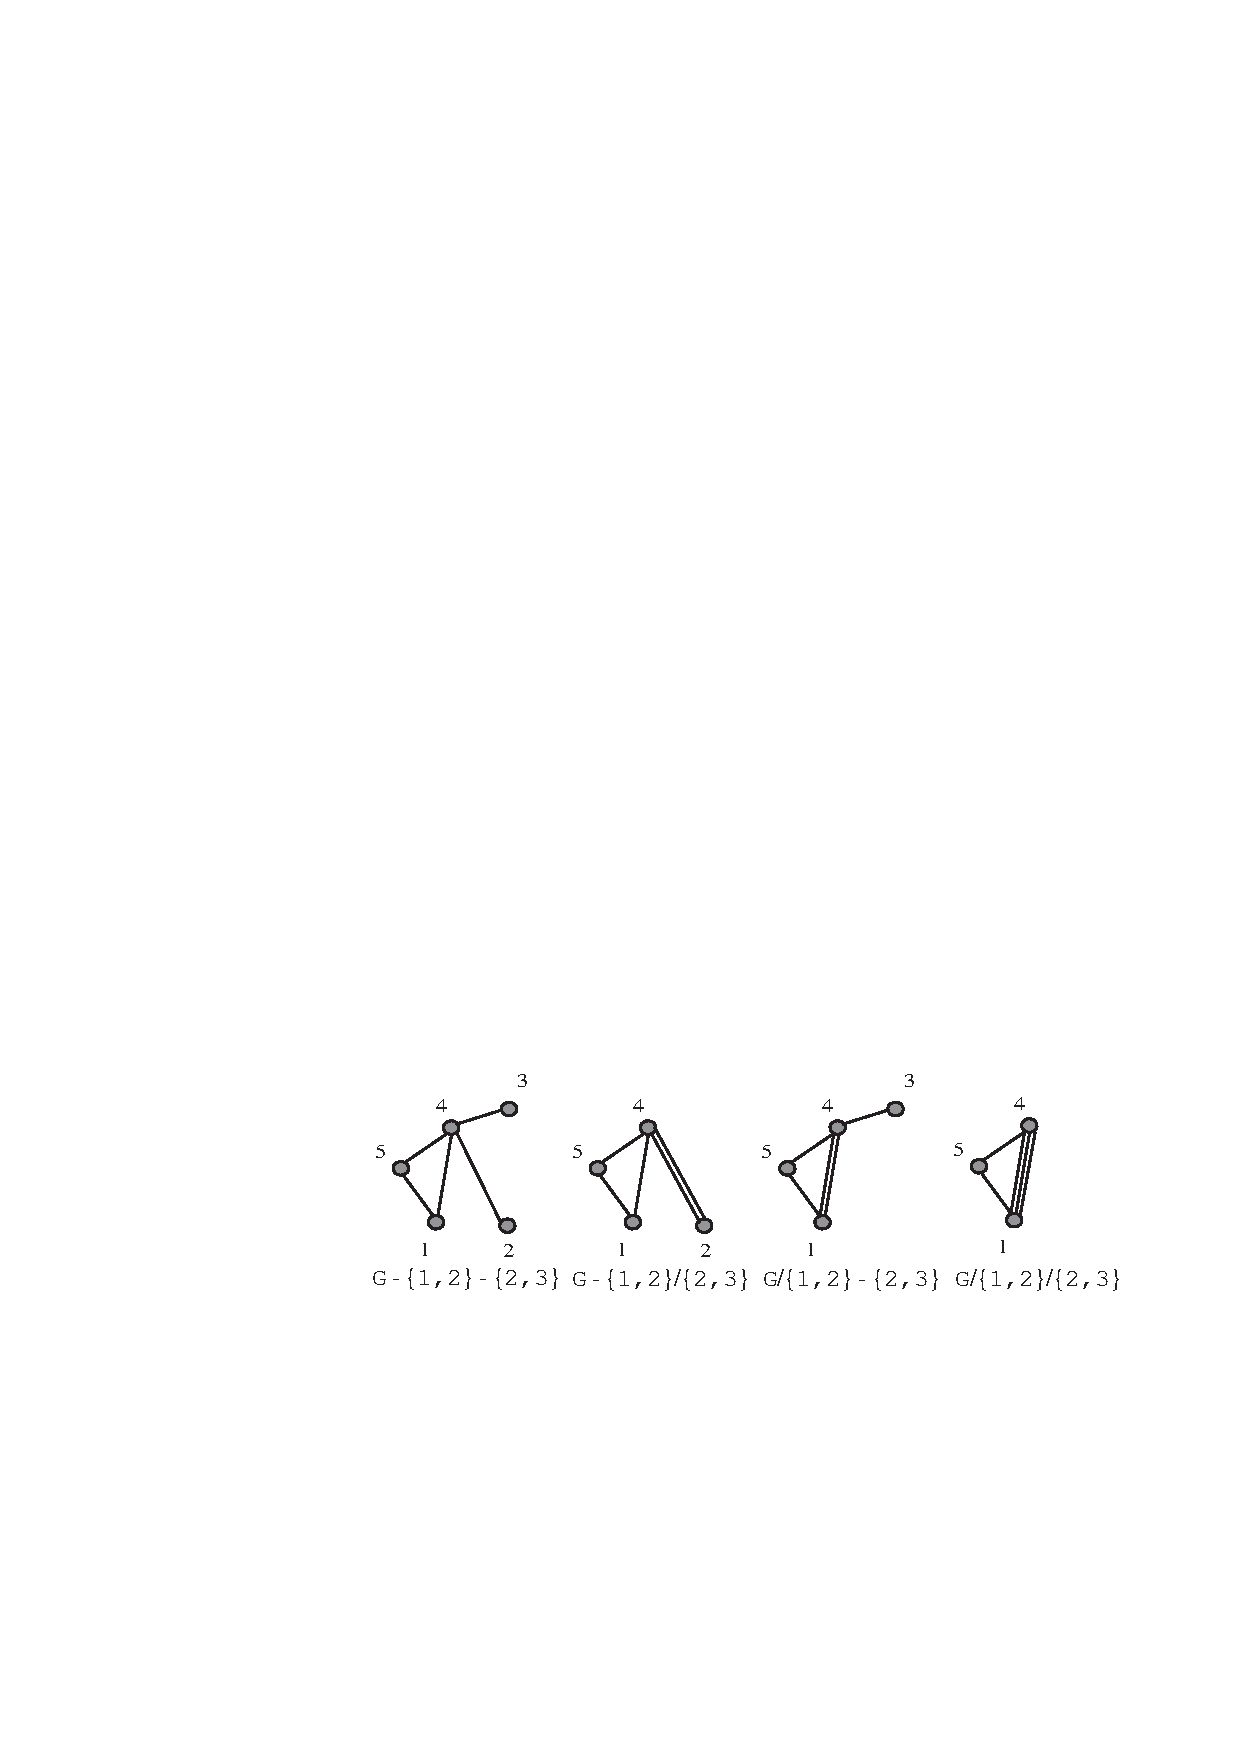
\includegraphics[width=0.95\linewidth]{images/spantreeexerciseresult}
\caption{Graphs obtained through deletions and contractions\label{delete-contract}}
\end{figure}
The chromatic polynomial of a triangle is \(x(x-1)(x-2)\) because for one vertex we have \(x\) colors, for a second we have \(x-1\), and for the third vertex, because it is adjacent to both of the other vertices, we have \(x-2\) choices of colors. For a vertex of degree 1 there are \(x-1\) choices of colors, those colors not used on the one vertex it is adjacent to. As we mentioned, the extra edges do not change the chromatic polynomial, so we have that the chromatic polynomial of \((G-\{1,2\})-\{2,3\}\) is \(x(x-1)^3(x-2)\), the chromatic polynomial of \((G-\{1,2\})/\{2,3\}\) is \(x(x-1)^2(x-2)\), as is that of \((G-\{2,3\})/\{1,2\}\), and the chromatic polynomial of \((G/\{2,3\})/\{1,2\}\) is \((x-1)(x-2)(x-3)\). Using the deletion-contraction recurrence, we get that%
\begin{align*}
\chi_G(x) \amp =\amp  \chi_{G-\{1,2\}}(x) - \chi_{G/\{1,2\}}(x)\\
\amp =\amp
\chi_{G-\{1,2\}-\{2,3\}}(x)-\chi_{(G-\{1,2\})/\{2,3\}}(x)-
\chi_{(G/\{1,2\})-\{2,3\}}(x)\\
\amp +\amp  \chi_{G/\{1,2\}/\{2,3\}}(x)\\
\amp =\amp  x(x-1)^3(x-2)-2x(x-1)^2(x-2) + x(x-1)(x-2)\\
\amp =\amp  x(x-1)(x-2)(x^2-2x+1 +2x-2 +1)\\
\amp =\amp  x^3(x-1)(x-2)
\end{align*}
for the chromatic polynomial of \(G\).%

\end{enumerate}
\begin{figure}
\centering
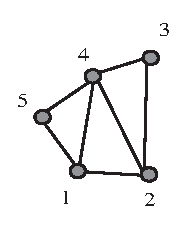
\includegraphics[width=0.73\linewidth]{images/spantreeexercise}
\caption{A graph.\label{del-cont}}
\end{figure}
\end{activity}
\begin{activity}[]\label{activity-224}
~\par
\begin{enumerate}[label=(\alph*)]
 \item In how many ways may you properly color the vertices of a path on \(n\) vertices with \(x\) colors? Describe any dependence of the chromatic polynomial of a path on the number of vertices. In how many ways may you properly color the vertices of a cycle on \(n\) vertices with \(x\) colors? Describe any dependence of the chromatic polynomial of a cycle on the number of vertices.%
\par\medskip\noindent%
\textbf{Solution.}\quad To color the vertices of a path, start at one end. There are \(x\) colors for that vertex, and \(x-1\) colors for each of the next \(n-1\), since each of them must be different from the preceding one. Thus the chromatic polynomial of a path on \(n\) vertices is \(x(x-1)^{n-1}\). The dependence on the number of vertices appears in the exponent on \(x-1\). If we use \(C_n\) to stand for a path on \(n\) vertices and \(P_n\) to stand for a path on \(n\) vertices, then by the deletion-contraction recurrence, we may write%
\begin{align*}
\hspace{-.4 in}\chi_{C_n}(x) \amp =\amp
\chi_{P_n}(x)-\chi_{C_{n-1}}(x)\\
\amp =\amp \chi_{P_n}(x)-\chi_{P_{n-1}}(x)+\chi_{C_{n-2}}(x)\\
\amp =\amp
\chi_{P_n}(x)-\chi_{P_{n-1}}(x)+\chi_{P_{n-3}}(x)-
\cdots+(-1)^{n-3}(\chi_{P_3}(x)-\chi_{C_2}(x))\\
\amp =\amp x(x-1)^{n-1}-x(x-1)^{n-2}+x(x-1)^{n-3}\cdots\\
\amp +\amp (-1)^{n-3}[x(x-1)^2-x(x-1)]\\
\amp =\amp x(x-1)\sum_{i=0}^{n-2}(x-1)^i(-1)^{n-2-i}\\
\amp =\amp x(x-1)(-1)^{n-2}\sum_{i=0}^{n-2}(1-x)^i\\
\amp =\amp x(x-1)(-1)^{n-2}{1-(1-x)^{n-1}\over 1-(1-x)}\\
\amp =\amp (x-1)[(x-1)^{n-1}+(-1)^n].
\end{align*}
%
\par
Here the dependence on \(n\) is interesting; effectively, we are taking \((x-1)\) times the result of dropping the constant term from \((x-1)^{n-1}\).%

~\par
\item In how many ways may you properly color the vertices of a tree on \(n\) vertices with \(x\) colors?%
\par\medskip\noindent%
\textbf{Solution.}\quad Color an arbitrary vertex; you have \(x\) choices for the color of that vertex. No two vertices adjacent to it are adjacent (otherwise we'd have a cycle), so for for each of them you have \(x-1\) choices of colors. No two vertices adjacent to colored vertices are adjacent to each other, nor is one of them adjacent to two colored vertices (in either case you'd have a cycle), so for each of them you'd have \(x-1\) colors. You can continue this argument until all vertices are colored, so you have \(x(x-1)^{n-1}\) ways to color the vertices.%
\par
You can also prove by induction that the chromatic polynomial of a tree is \(x(x-1)^{n-1}\). This is clearly true if there is one vertex. Otherwise, choose a vertex of degree 1 in an \(n\)-vertex tree and remove it. You may inductively assume that the chromatic polynomial of the remaining tree is \(x(x-1)^{n-2}\). Now there are \(x-1\) choices for the color of the vertex you removed since it has degree 1, and so the chromatic polynomial of the tree is \(x(x-1)^{n-1}\). There is also an inductive argument in which you delete and contract an arbitrary edge.%

\end{enumerate}
\end{activity}
\begin{activity}[]\label{activity-225}
What do you observe about the signs of the coefficients of the chromatic polynomial of the graph in \hyperref[del-cont]{Figure~\ref{del-cont}}? What about the signs of the coefficients of the chromatic polynomial of a path? Of a cycle? Of a tree? Make a conjecture about the signs of the coefficients of a chromatic polynomial and prove it.%
\par\medskip\noindent%
\textbf{Solution.}\quad not all powers of \(x\) appear, but the signs alternate as the power of \(x\) increases; that is, the sign of \(x^i\) is opposite that of \(x^{i+1}\). More precisely, if \(c_i\) is the coefficient of \(x^i\), then \((-1)^{n-i}c_i\ge 0\). To prove this, note it is trivially true for a graph with no edges. Choose an edge \(e\) of \(G\). Then \(\chi_G(x) =
\chi_{G-e}(x)-\chi_{G/e}(x)\). In \(G-e\), we may assume inductively that \((-1)^{n-i}c'_i\ge0\) and in \(G-/e\) we can assume inductively that \(c''_i(-1)^{n-1-i}\ge0\), where we use \(c'_i\) and \(c''_i\) as the coefficient of \(x^i\) in \(\chi_{G-e}(x)\) and \(\chi_{G/e}(x)\), respectively. Then \(c_i=c'_i
-c''_i\), and%
\begin{equation*}
c_i(-1)^{n-i}=c'_i(-1)^{n-i}-c''_i(-1)^{n-i}=c'_i(-1)^{n-i}+c''_i(-1)^{n-1-i}
\ge0.
\end{equation*}
%
\par
Therefore by the principle of mathematical induction, \(c_i(-1)^i\ge0\) for all finite graphs.%
\end{activity}
\typeout{************************************************}
\typeout{Section 4.2 Supplementary Problems}
\typeout{************************************************}
\section[{Supplementary Problems}]{Supplementary Problems}\label{sec_inclexcl-suppprobs}
\begin{activity}[]\label{activity-226}
Each person attending a party has been asked to bring a prize. The person planning the party has arranged to give out exactly as many prizes as there are guests, but any person may win any number of prizes. If there are \(n\) guests, in how many ways may the prizes be given out so that nobody gets the prize that he or she brought?%
\par\medskip\noindent%
\textbf{Solution.}\quad We use inclusion and exclusion. Property \(P_i\) is that person \(i\) gets the prize he or she brought. We are interested in \(N_{\mbox{e} }(\emptyset)\). If \(P\) is the set of all properties, we need to compute \(N_{\mbox{a} }(S)\) for every subset \(S\) of \(P\). But \(N_{\mbox{a} }(S)\) is the number of functions from the prizes to the people that give each prize represented by a property in \(S\) to the person who brought it. Think in terms of distributing those prizes first. Then there are \(n-|S|\) other prizes that we may pass out to the \(n\) people as we please, so we may do that in \(n^{n-|S|}\) ways. Thus \(N_{\mbox{a} }(S)=n^{n-|S|}\). Applying \hyperref[incexempty]{Equation~(\ref{incexempty})}, we get%
\begin{equation*}
N_{\mbox{e} }(\emptyset)=\sum_{S:s\subseteq P}(-1)^{|S|} n^{n-|S|} =
\sum_{s=0}^n (-1)^{|S|}\binom{n}{s}n^{n-s}.
\end{equation*}
%
\end{activity}
\begin{activity}[]\label{activity-227}
There are \(m\) students attending a seminar in a room with \(n\) seats. The seminar is a long one, and in the middle the group takes a break. In how many ways may the students return to the room and sit down so that nobody is in the same seat as before?%
\par\medskip\noindent%
\textbf{Solution.}\quad We use inclusion and exclusion. We let property \(P_i\) be the property that student \(i\) sits in the same seat as before. We are interested in \(N_{\mbox{e} }(\emptyset)\). For this purpose, for each subset \(S\) of the set \(P\) of all properties, we need to compute \(N_{\mbox{a} }(S)\), the number of ways for the students to return so that every student represented by a property in \(S\) sits in his or her previous seat. This leaves us with \(n-|S|\) seats to be filled in a one-to-one fashion in \(m-|S|\) students. There are \((n-|S|)^{\underline{m-|S|}}\) such seating arrangements, so \(N_{\mbox{a} }(S)= (n-|S|)^{\underline{m-|S|}}\). Thus we have%
\begin{equation*}
N_{\mbox{e} }(\emptyset)=\sum_{S:S\subseteq P}
(-1)^{|S|}(n-|S|)^{\underline{m-|S|}} = \sum_{s=0}^m (-1)^s\binom{m}{s}(n-s)^{\underline{m-s}}
\end{equation*}
ways for the students to return so that nobody sits in his or her previous place.%
\end{activity}
\begin{activity}[]\label{activity-228}
What is the number of ways to pass out \(k\) pieces of candy from an unlimited supply of identical candy to \(n\) children (where \(n\) is fixed) so that each child gets between three and six pieces of candy (inclusive)? If you have done \hyperref[candy-genfn]{Activity~\ref{candy-genfn}} compare your answer in that problem with your answer in this one.%
\par\medskip\noindent%
\textbf{Solution.}\quad As an inclusion-exclusion problem, we would let property \(i\) be that child \(i\) gets more than six pieces of candy. We would then observe that the number of ways to pass out the candy so that the children determined by a set \(S\) of properties all get more than six pieces, and everyone else gets at least 3, is the number of ways to pass out the remaining candy after giving 7 pieces to each child identified by \(S\) and 3 pieces to each other child. This number is \(\binom{k-7|S|-3(n-|S|)-1}{n-1}=\binom{k-2n-4|S|-1}{n-1}\). From here we would substitute into \hyperref[incexempty]{Equation~(\ref{incexempty})}, make any simplifications we could, and we would be done.%
\end{activity}
\begin{activity}[]\label{activity-229}
In how many ways may \(k\) distinct books be arranged on \(n\) shelves so that no shelf gets more than \(m\) books?%
\par\medskip\noindent%
\textbf{Solution.}\quad We use inclusion and exclusion. Let property \(P_i\) be that shelf \(i\) gets more than \(m\) books. Then the number of arrangements of books with at least the properties in a subset \(S\) of the set \(P\) of all properties is \(N_{\mbox{a} }(S) = k^{\underline{(m+1)|S|}}n^{\underline{k-(m+1)|S|}}\), because in order to have at least the properties in \(S\) we may choose \((m+1)|S|\) books and arrange \(m+1\) of them on each of the shelves represented by the properties in \(S\), after which we arrange the remainder of the books. Thus%
\begin{equation*}
N_{\mbox{e} }(\emptyset)=\sum_{S:S\subseteq P} (-1)^{|S|}
k^{\underline{(m+1)|S|}}n^{\underline{k-(m+1)|S|}}=\sum_{s=0}^n
(-1)^s\binom{n}{s}k^{\underline{(m+1)s}}n^{\underline{k-(m+1)s}}
\end{equation*}
is the number of ways to arrange the books so that no shelf gets more than \(m\).%
\end{activity}
\begin{activity}[]\label{activity-230}
Suppose that \(n\) children join hands in a circle for a game at nursery school. The game involves everyone falling down (and letting go). In how many ways may they join hands in a circle again so that nobody is to the right of the same child that was previously to his or her right?%
\par\medskip\noindent%
\textbf{Solution.}\quad We use inclusion and exclusion, with property \(i\) being the property that child \(i\) has the same child to the right the second time they join hands.  Given a set \(S\) of properties, we can think of arranging units consisting of individual children and strings of children holding hands in a circle. If we have \(s\) properties, then we have \(n-s\) of these units. Each string of children can be arranged in only one way, because our set specifies who has to have the same child on the right. Thus \(N_{\mbox{a} }(S) = (n-s-1)!\). This gives us%
\begin{align*}
N_{\mbox{e} }(\emptyset)=\sum_{S:S\subseteq P}
(-1)^{|S|}(n-|S|-1)!\amp =\amp 
\sum_{s=0}^n (-1)^s \binom{n}{s} (n-s-1)!\\
\amp =\amp \sum_{s=0}^n (-1)^s {n!\over
s!(n-s)}
\end{align*}
ways for the children to join hands the second time so that none of them has the same child to the right.%
\end{activity}
\begin{activity}[]\label{Hora}
Suppose that \(n\) people link arms in a folk-dance and dance in a circle. Later on they let go and dance some more, after which they link arms in a circle again. In how many ways can they link arms the second time so that no-one is next to a person with whom he or she linked arms before.%
\par\medskip\noindent%
\textbf{Solution.}\quad We use the Principle of Inclusion and Exclusion. Property \(P_i\) will be the property that person \(i\) links arms with someone previously to his or her right. (Saying it is the person to the right gives us more control over our formulas.) Given a subset \(S\) of the set \(P\) of all properties, the number of ways for the people in that set to link arms with the people previously on their right is the number of ways to arrange \(n-|S|\) strings of people around a circle with strings of length more than 1 having two ways to arrange themselves.  (Once we have two or more people linked, another person can be added to this string only at one end or not at all, because this person must have been to the right of one of the people on an end of the string. However a string of length two or more can unlink and then link in the opposite order, and each person will still be linked to exactly the same people.) Thus \(N_{\mbox{a} }(S)= (n-|S|-1)!2^{m(S)}\), where \(m(S)\) is the number of strings of length more than one determined by \(S\). The number \(m(S)\) can be any number from 1 to \(S\), so long as \(S\) is not too big; namely so long as \(|S|\le \lfloor n/1\rfloor\). (This is because if \(m(S)=|S|\), then each person determined by a property in \(S\) must be adjacent to a person not determined by a property in \(S\).) In particular, \(N_{\mbox{a} }(S)\) is not completely determined by the size of \(S\), as in all our other inclusion-exclusion problems. How do we compute \(m(S)\)? Let us call a subset \(R\) of \(S\) a run if \leavevmode%
\begin{enumerate}
\item\hypertarget{li-80}{}the people determined by \(R\) sit together in a row in both seatings, and%
\item\hypertarget{li-81}{}no other person in \(S\) is in a row with these people in both seatings.%
\end{enumerate}
 Some runs might determine just one person, but a run could also equal all of \(S\). Each run will have one more person not in \(S\) who was originally to the right of the person in the run who was rightmost in the first seating, and so this person will have to sit in a row with the people in \(R\) in the second seating as well. Thus the number \(r\) of runs in \(S\) is the number of strings \(m(S)\) that may be seated in two ways, and there are \(n-|S|-r\) people who do not have to be seated with runs. Thus \(N_{\mbox{a} }(S) = (n-|S|-1)!2^r\), because the total number of strings of people (including strings of just one person) we need to seat is \(n-|S| -r\), and there are \((k-1)!\) ways to arrange \(k\) objects in a circle.. If we try to use the information we have so far to compute \(N_{\mbox{e} }(\emptyset)\), we get%
\begin{equation*}
N_{\mbox{e} }(\emptyset)=\sum_{S:S\subseteq P}(-1)^{|S|}(n-|S|_1)!2^r
=\sum_{s=0}^n\sum_{r=1}^{|S|}N(s,r)(n-s-1)!2^r,
\end{equation*}
in which \(N(s,r)\) stands for the number of property sets with size \(s\) and \(r\) runs.%
\par
Picking out runs in a circular arrangement adds a layer of difficulty, so to compute \(N(s,r)\), we first compute how many subsets of \([n]\) we have with \(r\) runs and then adjust for putting \(1\) through \(n\) around a circle in order.  Imagine writing 1 through \(n\) in a straight line, each integer occupying one unit of distance along the line. We now place \(r\) sticks whose lengths add to \(s\) (each stick has positive integer length) along that line. Each stick picks out a set of consecutive integers, as many as its length, so the sticks together pick out \(s\) integers. In order to be sure the sticks correspond to runs, we need to make sure they do not touch each other, so we place \(n-s\) identical stones along the line too, making sure there is at least one stone between any two sticks. The stones thus pick out the integers not in \(S\). The sticks are not quite identical, though the sticks of a given length are. In other words, which lengths of sticks are in which places is what matters. So the sticks give us a composition of \(s\), a list of distinct positive integers that add to \(s\). We know there are \(\binom{s-1}{r-1}\) such compositions. Once we have chosen an ordering for the sticks, we need to distribute the stones among the sticks so that no two sticks are adjacent.  Since the stones are identical, we can do this by putting one stone between each pair of sticks in our composition, and then distribute the remaining \(n-s-r+1\) stones in any way we want among the \(r-1\) places between the sticks and the two places to the left and right of all the sticks.. We can do this in%
\begin{equation*}
\binom{r+1 + (n-s-r+1)-1}{n-s-r+1}=\binom{n-s+1}{n-s-r+1}=\binom{n-s+1}{r}
\end{equation*}
ways. Thus there are \(\binom{s-1}{r-1}\binom{n-s+1}{r}\) ways to choose a subset \(S\) of \([n]\) that has \(r\) runs.%
\par
Now we have to deal with the fact that our \(n\) people (who we have replaced with the integers 1 through \(n\) in order) were arranged around a circle. That means that a run is now a set of consecutive integers on the circle, where \(n\) and 1 are considered consecutive. Recall that the set \(S\) is picked out by the sticks. If we arrange 1 through \(n\) around a circle in order, the set \(S\) that originally had \(r\) runs will have \(r-1\) runs if sticks covered both the first and last integer (1 and \(n\)), but otherwise it will still have \(n\) runs. Thus the number of subsets of \([n]\) that have \(n\) runs when \(1\) through \(n\) are arranged in a circle is the number of subsets of \([n]\) with \(r+1\) runs that have both 1 and \(n\) in \(S\) plus the number of subsets of \([n]\) with \(r\) runs that do not have both \(1\) and \(n\) in \(S\). To compute the number of subsets \(S\) that \emph{do} contain both 1 and \(n\), we compute the number of arrangements of \(r\) sticks and \(n-s\) stones that do start and end with a stick; that means that after we choose our composition into \(r\) parts to get our arrangement of sticks and place one stone between each pair of previously adjacent sticks, we now place the remaining \(n-s-r+1\) stones in the \(r-1\) places between previously adjacent sticks in%
\begin{equation*}
\binom{r-1 + (n-s-r+1)-1}{n-s-r+1}=\binom{n-s-1}{n-s-r+1}=\binom{n-s-1}{r-2}
\end{equation*}
ways. For the sticks and stones to determine a subset we must assign lengths to the sticks; the number of ways to do this is, as above, \(\binom{s-1}{r-1}\), the number of compositions of \(s\) with \(r\) parts. Thus there are \(\binom{s-1}{r-1}\binom{n-s-1}{r-2}\) subsets of \([n]\) that have \(r\) runs and include both 1 and \(n\). For our computation we will also want the number of subsets of \([n]\) that have \(r+1\) runs and contain both \(1\) and \(n\) this is \(\binom{s-1}{r}\binom{n-s-1}{r-1}\).%
\par
On the other hand, the number of subsets of \([n]\) that have \(r\) runs and do not contain both \(1\) and \(n\) is the total number of subsets with \(r\) runs minus the number that do contain both \(1\) and \(n\); this is%
\begin{equation*}
\binom{s-1}{r-1}\left(\binom{n-s+1}{r}- \binom{n-s-1}{r-2}\right).
\end{equation*}
%
\par
This gives us%
\begin{equation*}
N(s,r) =\binom{s-1}{r}\binom{n-s-1}{r-1}+\binom{s-1}{r-1}\left(\binom{n-s+1}{r}- \binom{n-s-1}{r-2}\right)
\end{equation*}
ways to choose an \(s\)-element subset of \([n]\) that has \(r\) runs when \([n]\) is arranged around a circle. Thus there are \(\sum\limits_{s=0}^n\sum\limits_{r=1}^{s}(-1)^s\left[\binom{s-1}{r}\binom{n-s-1}{r-1}+\binom{s-1}{r-1}\left(\binom{n-s+1}{r}- \binom{n-s-1}{r-2}\right)\right](n-s-1)!2^r\) ways for people to arrange themselves in the second circle so that no-one is adjacent to anyone he or she was previously adjacent to.%
\end{activity}
\begin{activity}[]\label{activity-232}
(A challenge; the author has not tried to solve this one!) Redo \hyperref[Hora]{Problem~\ref{Hora}} in the case that there are \(n\) men and \(n\) women and when people arrange themselves in a circle they do so alternating gender.%
\end{activity}
\begin{activity}[]\label{activity-233}
Suppose we take two graphs \(G_1\) and \(G_2\) with disjoint vertex sets, we choose one vertex on each graph, and connect these two graphs by an edge \(e\) to get a graph \(G_{12}\). How does the chromatic polynomial of \(G_{12}\) relate to those of \(G_1\) and \(G_2\)?%
\par\medskip\noindent%
\textbf{Solution.}\quad By the deletion-contraction recurrence,%
\begin{equation*}
\chi_{G_{12}}(x) =
\chi_{G_{12}-e}(x)-\chi_{G_{12/e}}(x).
\end{equation*}
%
\par
Now \(\chi_{G_{12}-e}(x)=\chi_{G_1}(x)\times \chi_{G_2}(x)\) because each ordered pair of proper colorings of \(G_1\) and \(G_2\) is a proper coloring of \(G_{12}-e\). \(G_{12}/e\) is the graph we get by identifying the endpoint of \(e\) in \(G_1\) with the endpoint of \(e\) in \(G_2\). Notice that if you fix one vertex of a graph \(G\), fix one color, and ask how many proper colorings with \(x\) colors \(G\) has in which the fixed vertex is the fixed color, you get \(\chi_G(x)/x\).  (By the quotient principle.) Thus \(\chi_{G_2}(x)/x\) is the number of ways to extend a proper coloring of \(G_1\) to a proper coloring of \(G_{12}/e\). Then, by the product principle, the number of proper colorings of \(G_{12}/e\) with \(x\) colors is \(\chi_{G_1}(x)\chi_{G_2}(x)/x\). Therefore by the deletion-contraction recurrence, \(\chi_{G_{12}}(x) = \chi_{G_1}(x)\chi_{G_2}(x)(1-{1\over x})\).%
\end{activity}
\typeout{************************************************}
\typeout{Chapter 5 Groups acting on sets}
\typeout{************************************************}
\chapter[{Groups acting on sets}]{Groups acting on sets}\label{groupsonsets}
\typeout{************************************************}
\typeout{Section 5.1 Permutation Groups}
\typeout{************************************************}
\section[{Permutation Groups}]{Permutation Groups}\label{sec_groups-permgroups}
\typeout{************************************************}
\typeout{Introduction  }
\typeout{************************************************}
Until now we have thought of permutations mostly as ways of listing the elements of a set. In this chapter we will find it very useful to think of permutations as functions. This will help us in using permutations to solve enumeration problems that cannot be solved by the quotient principle because they involve counting the blocks of a partition in which the blocks don't have the same size. We begin by studying the kinds of permutations that arise in situations where we have used the quotient principle in the past.%
\typeout{************************************************}
\typeout{Subsection  The rotations of a square}
\typeout{************************************************}
\subsection[{The rotations of a square}]{The rotations of a square}\label{subsection-57}
\leavevmode%
\begin{figure}
\centering
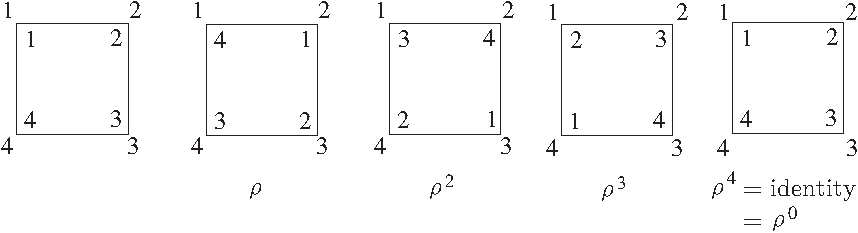
\includegraphics[width=0.95\linewidth]{images/RotationsOfSquare}
\caption{The four possible results of rotating a square and maintaining its position.\label{RotationsOfSquare}}
\end{figure}
In \hyperref[RotationsOfSquare]{Figure~\ref{RotationsOfSquare}} we show a square with its four vertices labelled 1, 2, 3, and 4. We have also labeled the spot in the plane where each of these vertices falls with the same label. Then we have shown the effect of rotating the square clockwise through 90, 180, 270, and 360 degrees (which is the same as rotating through 0 degrees). Underneath each of the rotated squares we have named the function that carries out the rotation. We use \(\rho\), the Greek letter pronounced ``row,'' to stand for a 90 degree clockwise rotation. We use \(\rho^2\) to stand for two 90 degree rotations, and so on. We can think of the function \(\rho\) as a function on the four element set\footnote{What we are doing is restricting the rotation \(\rho\) to the set \(\{1,2,3,4\}\).\label{fn-17}} \(\{1,2,3,4\}\). In particular, for any function \(\varphi\) (the Greek letter phi, usually pronounced ``fee,'' but sometimes ``fie'') from the plane back to itself that may move the square around but otherwise leaves it in the same place, we let \(\varphi(i)\) be the label of the place where vertex previously in position \(i\) is now. Thus \(\rho(1) =2\), \(\rho(2)=3\), \(\rho(3)=4\) and \(\rho(4) =1\). Notice that \(\rho\) is a permutation on the set \(\{1,2,3,4\}\).%
\begin{activity}[]\label{activity-234}
Find \(\rho^2\) of 1, 2, 3, and 4. Find \(\rho^3\) of 1, 2, 3, and 4. Are \(\rho^2\) and \(\rho^3\) permutations of \(\{1,2,3,4\}\)?%
\par\medskip\noindent%
\textbf{Solution.}\quad \(\rho^2(1)=3\), \(\rho^2(2)=4\), \(\rho^2(3)=1\), \(\rho^2(4) =2\). \(\rho^3(1)=4\), \(\rho^3(2)=1\), \(\rho^3(3)=2\), \(\rho^3(4)=3\). Yes, \(\rho^2\) and \(\rho^3\) are permutations of \(\{1,2,3,4\}\).%
\end{activity}
\begin{activity}[]\label{composition1}
The composition\index{composition of functions}\index{functions!composition of} \(f\circ g\) of two functions \(f\) and \(g\) is defined by \(f\circ g(x) = f(g(x))\). Is \(\rho^3\) the composition of \(\rho\) and \(\rho^2\)? Does the answer depend on the order in which we write \(\rho\) and \(\rho^2\)? How is \(\rho^2\) related to \(\rho\)?%
\par\medskip\noindent%
\textbf{Solution.}\quad Yes, \(\rho^3\) is the composition of \(\rho\) and \(\rho^2\), and also of \(\rho^2\) and \(\rho\), so it doesn't matter in which order we write them. \(\rho^2=\rho\circ\rho\).%
\end{activity}
\begin{activity}[]\label{activity-236}
Is the composition of two permutations always a permutation?%
\par\medskip\noindent%
\textbf{Solution.}\quad Yes, because the composition of one-to-one functions is one-to-one and the composition of onto functions is onto.%
\end{activity}
In \hyperref[composition1]{Problem~\ref{composition1}} you see that we can think of \(\rho^2\circ\rho\) as the result of first rotating by 90 degrees and then by another 180 degrees. In other words, the composition of two rotations is the same thing as first doing one and then doing the other. If we first rotate by 90 degrees and then by 270 degrees then we have rotated by 360 degrees, which does nothing visible to the square. Thus we say that \(\rho^4\) is the ``identity function.'' In general the \emph{identity function}\index{function!identity}\index{identity function} on a set \(S\), denoted by \(\iota\) (the Greek letter iota, pronounced eye-oh-ta) is the function that takes each element of the set to itself. In symbols, \(\iota(x) =x\) for every \(x\) in \(S\). Of course the identity function on a set is a permutation of that set.%
\typeout{************************************************}
\typeout{Subsection  Groups of Permutations}
\typeout{************************************************}
\subsection[{Groups of Permutations}]{Groups of Permutations}\label{subsection-58}
\begin{activity}[]\label{activity-237}
For any function \(\varphi\) from a set \(S\) to itself, we define \(\varphi^n\) (for nonnegative integers \(n\)) inductively by \(\varphi^0 =
\iota\) and \(\varphi^n = \varphi^{n-1}\circ\varphi\) for every positive integer \(n\). If \(\varphi\) is a permutation, is \(\varphi^n\) a permutation? Based on your experience with previous inductive proofs, what do you expect \(\varphi^n\circ \varphi^m\) to be? What do you expect \((\varphi^m)^n\) to be? There is no need to prove these last two answers are correct, for you have, in effect, already done so in Chapter 2.%
\par\medskip\noindent%
\textbf{Solution.}\quad It is a permutation because the computation of permutations is a permutation. (You could be more precise and use the inductive definition of \(\varphi^n\) to prove inductively that \(\varphi^n\) is a permutation.) We expect \(\varphi^m\circ\varphi^n=\varphi^{m+n}\), and we expect \((\varphi^m)n=\varphi^{mn}\), and we would prove this by induction.%
\end{activity}
\begin{activity}[]\label{identityproperty}
If we perform the composition \(\iota\circ \varphi\) for any function \(\varphi\) from \(S\) to \(S\), what function do we get? What if we perform the composition \(\varphi\circ\iota\)?%
\par\medskip\noindent%
\textbf{Solution.}\quad \(\iota\circ\varphi=\varphi\circ\iota=\varphi\)%
\end{activity}
What you have observed about iota in \hyperref[identityproperty]{Problem~\ref{identityproperty}} is called the \emph{identity property}\index{identity property (for permutations)} of iota. In the context of permutations, people usually call the function \(\iota\) ``the identity'' rather than calling it ``iota.''%
\par
Since rotating first by 90 degrees and then by 270 degrees has the same effect as doing nothing, we can think of the 270 degree rotation as undoing what the 90 degree rotation does. For this reason we say that in the rotations of the square, \(\rho^3\) is the ``inverse'' of \(\rho\). In general, a function \(\varphi:T\rightarrow S\) is called an \emph{inverse}\index{inverse function}\index{function!inverse} of a function \(\sigma:S
\rightarrow T\) (the lower case Greek letter sigma) if \(\varphi\circ \sigma= \sigma
\circ\varphi =
\iota\).%
\begin{activity}[]\label{activity-239}
Does every permutation have an inverse? If so, why, and is it unique, i.e. could a permutation have two distinct inverse functions? If not, give an example of a permutation without an inverse or a permutation with two distinct inverses.%
\par\medskip\noindent%
\textbf{Solution.}\quad Let \(\varphi\) be a permutation of \(S\). Then for each \(S\) in \(S\) there is one and only one \(x\) in \(S\) such that \(\varphi(x) = s\) because \(\varphi\) is one-to-one and onto. Thus if we define \(\sigma(s)\) to be the unique \(x\) such that \(\varphi(x) = s\), we have defined a function, and%
\begin{equation*}
\varphi\circ\sigma (s) = \varphi(\sigma(s)) = \varphi(x) = s.
\end{equation*}
%
\par
Thus we have that \(\varphi\circ\sigma = \iota\). To show that \(\sigma\) is an inverse to \(\varphi\), we must show that \(\sigma\circ\varphi = \iota\) as well. However \(\sigma(\varphi(y))\) is the unique \(x\) such that \(\varphi(x) = \varphi(y)\), that is \(\sigma(\varphi(y)) = y\). Thus \(\sigma\circ\varphi = \iota\), and \(\sigma\) is an inverse to \(\varphi\).%
\end{activity}
\begin{activity}[]\label{activity-240}
Show that if \(\sigma\) is an inverse of the permutation \(\varphi\) of \(S\), then \(\sigma\) is a permutation of \(S\) also.%
\par\medskip\noindent%
\textbf{Solution.}\quad The function \(\sigma\) must be one-to-one because if \(\sigma(x)=\sigma(y)\), then \(x=\varphi\circ\sigma(x)=\varphi\circ\sigma(y)=y\). The function \(\sigma\) must be onto because for each \(y\) in its range, \(\sigma(\varphi(y)) = y\)%
\end{activity}
We use \(\varphi^{-1}\) to denote the inverse of the permutation \(\varphi\). We've seen that the rotations of the square are functions that return the square to its original position but may move the vertices to different places. In this way we create permutations of the vertices of the square. We've observed three important properties of these permutations. \leavevmode%
\begin{itemize}[label=\textbullet]
\item{}(Identity Property)\index{identity property} These permutations include the identity permutation.%
\item{}(Inverse Property)\index{inverse property} Whenever these permutations include \(\varphi\), they also include \(\varphi^{-1}\).%
\item{}(Closure Property)\index{closure property}  Whenever these permutations include \(\varphi\) and \(\sigma\), they also include \(\varphi\circ\sigma\).%
\end{itemize}
%
\par
A set of permutations with these three properties is called a \emph{permutation group}\footnote{The concept of a permutation group is a special case of the concept of a \emph{group} that one studies in abstract algebra.  When we refer to a group in what follows, if you  know what groups are in the more abstract sense, you may use the word in this way. If you do not know about groups in this more abstract sense, then you may assume we mean permutation group when we say group.\label{fn-18}} or a group of permutations.\index{group of permutations}\index{permutation group} We will denote the group of permutations corresponding to rotations of the square by \(R_4\) and call it the \emph{rotation group}\index{rotation group} of the square. There is a similar rotation group with \(n\) elements for any regular \(n\)-gon.%
\begin{activity}[]\label{activity-241}
If a finite set of permutations satisfies the closure property is it a permutation group?%
\par\medskip\noindent%
\textbf{Solution.}\quad Yes, because the permutations \(\sigma\), \(\sigma^2\), \dots{}, \(\sigma^n\), \dots{} must eventually start repeating. But if \(\sigma^i=\sigma^j\), and \(i\lt j\), then \(\sigma^{j-i} =1\), so \(\sigma^{j-i-1}\) is the inverse of \(\sigma\). This means that every member of the set of permutations has an inverse in that set. But then since \(\sigma\circ\sigma^{-1} = \iota\), we have that the identity is in the set as well. Thus it is a permutation group.%
\end{activity}
\begin{activity}[]\label{activity-242}
~\par
\begin{enumerate}[label=(\alph*)]
 \item How should we define \(\varphi^{-n}\) for an element \(\varphi\) of a permutation group?%
\par\medskip\noindent%
\textbf{Solution.}\quad We define \(\varphi^{-n}=\left(\varphi^{-1}\right)^n\).%

~\par
\item Will the two standard rules for exponents%
\begin{equation*}
a^ma^n=a^{m+n} \mbox{\ and\ }  (a^m)^n = a^{mn}
\end{equation*}
still hold if one or more of the exponents may be negative?%
\par\medskip\noindent%
\textbf{Solution.}\quad Yes.%

~\par
\item What would we have to prove to show that the rules still hold?%
\par\medskip\noindent%
\textbf{Solution.}\quad To prove this we need to show that for nonnegative \(m\) and \(n\) we have that \(\varphi^m\circ\varphi^{-n} =
\varphi^{m-n}\), that \(\varphi^{-m}\varphi^{-n} = \varphi^{-m-n}\), that \((\varphi^m)^{-n} = \varphi^{-mn}\), that \((\varphi^{-m})^n = \varphi^{-mn}\) and that \((\varphi^{-m})^{-n}= \varphi^{mn}\).%

~\par
\item If the rules hold, give enough of the proof to show that you know how to do it; otherwise give a counterexample.%
\par\medskip\noindent%
\textbf{Solution.}\quad We give the first and last proof. We will induct on \(n\) in the first proof. If \(n=0\) the formula automatically holds. Assume inductively that \(\varphi^m\circ\varphi^{-(n-1)} = \varphi^{m-(n-1)}\). Compose both sides of this equation on the right by \(\sigma^{-1}\) and use the associative law for composition of functions to get, in the case that \(m-n\) is nonnegative%
\begin{align*}
\varphi^m\circ(\varphi^{-(n-1)}\circ\varphi^{-1}) \amp =\amp
\varphi^{m-(n-1)}\circ\varphi^{-1}\\
\varphi^m\circ(\varphi^{-1})^{n-1}\varphi^{-1}\amp =\amp
(\varphi^{m-n}\circ\varphi)\circ\varphi^{-1}\\
\varphi^m\circ(\varphi^{-1})^n \amp =\amp  \varphi^{m-n}.
\end{align*}
%
\par
We do the same in the case that \(m-n\) is negative, getting%
\begin{align*}
\varphi^m\circ(\varphi^{-(n-1)}\circ\varphi^{-1}) \amp =\amp
\varphi^{m-(n-1)}\circ\varphi^{-1}\\
\varphi^m\circ(\varphi^{-1})^{n-1}\varphi^{-1}\amp =\amp
(\varphi^{-1})^{n-m-1}\circ\varphi^{-1}\\
\varphi^m\circ(\varphi^{-1})^n \amp =\amp  (\varphi^{-1})^{n-m}\\
\varphi^m\circ\varphi^{-n}\amp =\amp \varphi^{m-n}.
\end{align*}
%
\par
To prove the last statement we need to prove, we write the following, in which the line {$\langle\langle$Unresolved xref, reference "crucialline"; check spelling or use "provisional" attribute$\rangle\rangle$} follows from the first equation we proved and the line {$\langle\langle$Unresolved xref, reference "modestlyimportant"; check spelling or use "provisional" attribute$\rangle\rangle$} follows from the fact that \((\varphi^{-1})^{-1} = \varphi\).%
\begin{align*}
(\varphi^{-m})^{-n} \amp =\amp  ([\varphi^{-1})^m]^{-1})^n\nonumber\\
\amp =\amp [(\varphi^{-1})^{-m}]^n\\
\amp =\amp ([(\varphi^{-1})^{-1}]^m)^n\nonumber\\
\amp =\amp (\varphi^m)^n\\
\amp =\amp \varphi^{mn}\nonumber
\end{align*}
%

\end{enumerate}
\end{activity}
\begin{activity}[]\label{dihedral1}
There are three dimensional geometric motions of the square that return it to its original position but move some of the vertices to other positions. For example, if we flip the square around a diagonal, most of it moves out of the plane during the flip, but the square ends up in the same place. Draw a figure like \hyperref[RotationsOfSquare]{Figure~\ref{RotationsOfSquare}} that shows all the possible results of such motions, including the ones shown in \hyperref[RotationsOfSquare]{Figure~\ref{RotationsOfSquare}}. Do the corresponding permutations form a group?%
\end{activity}
\begin{activity}[]\label{activity-244}
If \(f:S\rightarrow T\), \(g:T\rightarrow X\), and \(h:X \rightarrow Y\), is \(h\circ(g\circ f) = (h\circ g)\circ f\)? What does this say about the status of the \emph{associative law}\index{associative law}%
\begin{equation*}
\rho\circ(\sigma\circ \varphi) = (\rho\circ \sigma)\circ\varphi
\end{equation*}
in a group of permutations?%
\par\medskip\noindent%
\textbf{Solution.}\quad Since \((h\circ(g\circ f)) (x) = h((g\circ f)(x)) = h(g(f(x)))\) and \(((h\circ
g)\circ f) (x) = (h\circ g)(f(x)) = h(g(f(x)))\), we have that%
\begin{equation*}
h\circ (g\circ f) =
(h\circ g)\circ f.
\end{equation*}
%
\par
This says that the associative law holds for the composition operation in a group of permutations.%
\end{activity}
\begin{activity}[]\label{activity-245}
If \(\sigma\) and \(\varphi\) are permutations, why must \(\sigma\circ\varphi\) have an inverse? Is \((\sigma\circ\varphi)^{-1}=
\sigma^{-1}\varphi^{-1}\)? (Prove or give a counter-example.) Is \((\sigma\circ\varphi)^{-1}=
\varphi^{-1}\sigma^{-1}\)? (Prove or give a counter-example.)%
\par\medskip\noindent%
\textbf{Solution.}\quad One could either say that the composition of one-to-one and onto functions is one-to-one and onto, or note that \((\sigma\circ\varphi)\circ (\varphi^{-1}\circ
\sigma^{-1}) =\iota\) by the associative law. Note that this says that \((\sigma \circ
\varphi)^{-1}= \varphi^{-1}\circ \sigma^{-1}\). In the dihedral group \(D_4\), \(\rho^{-1}= \rho^3\) and \(\varphi_{1/3}^{-1} = \varphi{1/3}\). Thus%
\begin{align*}
(\rho\circ \varphi_{1/3})\circ (\rho^{-1}\circ
\varphi_{1/3}^{-1})\amp =\amp \rho\circ
\varphi_{1/3})\circ(\rho^3\varphi_{1/3})\\
\amp =\amp \varphi_{12/34}\circ \varphi_{14/23}\\
\amp =\amp \rho^2.
\end{align*}
%
\par
This shows that \((\sigma\circ\varphi)^{-1}\not=
\sigma^{-1}\varphi^{-1}\).%
\end{activity}
\begin{activity}[]\label{activity-246}
Explain why the set of all permutations of four elements is a permutation group. How many elements does this group have? This group is called the \emph{symmetric group on four letters}\index{symmetric group} and is denoted by \(S_4\).%
\par\medskip\noindent%
\textbf{Solution.}\quad It is a finite set of permutations that satisfies the closure property. It has \(4!= 24\) elements.%
\end{activity}
\typeout{************************************************}
\typeout{Subsection  The symmetric group}
\typeout{************************************************}
\subsection[{The symmetric group}]{The symmetric group}\label{subsection-59}
In general, the set of all permutations of an \(n\)-element set is a group. It is called the \emph{symmetric group on \(\mathbf n\) letters}\index{symmetric group}. We don't have nice geometric descriptions (like rotations) for all its elements, and it would be inconvenient to have to write down something like ``Let \(\sigma(1) =3\), \(\sigma(2) =1\), \(\sigma(3)=4\), and \(\sigma(4)=1\)'' each time we need to introduce a new permutation. We introduce a new notation for permutations that allows us to denote them \emph{reasonably} compactly and compose them reasonably quickly. If \(\sigma\) is the permutation of \(\{1,2,3,4\}\) given by \(\sigma(1)=3\), \(\sigma(2)=1\), \(\sigma(3) =4\) and \(\sigma(4) =2\), we write%
\begin{equation*}
\sigma =\left( \begin{matrix}1\amp 2\amp 3\amp 4\cr3\amp 1\amp 4\amp 2
\end{matrix} \right).
\end{equation*}
%
\par
We call this notation the \emph{two row notation}\index{permutation!two row notation}\index{two row notation} for permutations. In the two row notation for a permutation of \(\{a_1,a_2,\ldots, a_n\}\), we write the numbers \(a_1\) through \(a_n\) in a one row and we write \(\sigma(a_1)\) through \(\sigma(a_n)\) in a row right below, enclosing both rows in parentheses. Notice that%
\begin{equation*}
\left( \begin{matrix}1\amp 2\amp 3\amp 4\cr3\amp 1\amp 4\amp 2
\end{matrix} \right) = \left(
\begin{matrix}2\amp 1\amp 4\amp 3\cr1\amp 3\amp 2\amp 4
\end{matrix} \right),
\end{equation*}
although the second ordering of the columns is rarely used.%
\par
If \(\varphi\) is given by%
\begin{equation*}
\varphi = \begin{pmatrix}1\amp 2\amp 3\amp 4\cr4\amp 1\amp 2\amp 3
\end{pmatrix} ,
\end{equation*}
then, by applying the definition of composition of functions, we may compute \(\sigma\circ
\varphi\) as shown in \hyperref[permutationproduct]{Figure~\ref{permutationproduct}}.%
\begin{figure}
\centering
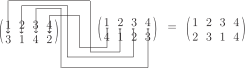
\includegraphics[width=0.73\linewidth]{images/productofpermutations}
\caption{How to multiply permutations in two-row notation.\label{permutationproduct}}
\end{figure}
We don't normally put the circle between two permutations in two row notation when we are composing them, and refer to the operation as multiplying the permutations, or as the product of the permutations. To see how \hyperref[permutationproduct]{Figure~\ref{permutationproduct}} illustrates composition, notice that the arrow starting at 1 in \(\varphi\) goes to 4. Then from the 4 in \(\varphi\) it goes to the 4 in \(\sigma\) and then to 2. This illustrates that \(\varphi(1)=4\) and \(\sigma(4) =2\), so that \(\sigma(\varphi(1))=2\).%
\begin{activity}[]\label{activity-247}
For practice, compute \(\begin{pmatrix}1\amp 2\amp 3\amp 4\amp 5\cr3\amp 4\amp 1\amp 5\amp 2
\end{pmatrix}
\begin{pmatrix}1\amp 2\amp 3\amp 4\amp 5\cr 4\amp 3\amp 5\amp 1\amp 2
\end{pmatrix}\).%
\par\medskip\noindent%
\textbf{Solution.}\quad \(\begin{pmatrix}1\amp 2\amp 3\amp 4\amp 5\cr5\amp 1\amp 2\amp 3\amp 4
\end{pmatrix}\)%
\end{activity}
\typeout{************************************************}
\typeout{Subsection  The dihedral group}
\typeout{************************************************}
\subsection[{The dihedral group}]{The dihedral group}\label{subsection-60}
We found four permutations that correspond to rotations of the square. In \hyperref[dihedral1]{Problem~\ref{dihedral1}} you found four permutations that correspond to flips of the square in space. One flip fixes the vertices in positions 1 and 3 and interchanges those in positions 2 and 4. (Notice we did not say it fixes the vertices labelled 1 and 3.)\footnote{There is room for tremendous confusion here, and professional mathematicians sometimes suffer from it.  Just try to remember that when we describe the axis of a flip, we describe it relative to points given in space, not points on the square or other object we are flipping.\label{fn-19}} Let us denote it by \(\varphi_{1/3}\). One flip fixes the vertices in positions 2 and 4 and interchanges those in positions 1 and 3. Let us denote it by \(\varphi_{2/4}\). One flip interchanges the vertices in positions 1 and 2 and also interchanges those in positions 3 and 4. Let us denote it by \(\varphi_{12/34}\). The fourth flip interchanges the vertices in positions 1 and 4 and interchanges those in positions 2 and 3. Let us denote it by \(\varphi_{14/23}\). Notice that \(\varphi_{1/3}\) is a permutation that takes vertex 1 to vertex 1 and vertex 3 to vertex 3, while \(\varphi_{12/34}\) is a permutation that takes the edge from 1 to 2 to the edge from 1 to 2 and takes the edge from 3 to 4 to the edge from 3 to 4.%
\begin{activity}[]\label{dihedral2}
~\par
\begin{enumerate}[label=(\alph*)]
 \item Write down the two-row notation for \(\rho^3\), \(\varphi_{2/4}\), \(\varphi_{12/34}\) and \(\varphi_{2/4}\circ \varphi_{12/34}\). Remember that \(\sigma(i)\) stands for the position where the vertex that originated in position \(i\) is after we apply \(\sigma\).%
\par\medskip\noindent%
\textbf{Solution.}\quad \(\begin{pmatrix}1\amp 2\amp 3\amp 4\cr4\amp 1\amp 2\amp 3
\end{pmatrix}\), \(\begin{pmatrix}1\amp 2\amp 3\amp 4\cr3\amp 2\amp 1\amp 4
\end{pmatrix}\), \(\begin{pmatrix}1\amp 2\amp 3\amp 4\cr2\amp 1\amp 4\amp 3
\end{pmatrix}\), \(\begin{pmatrix}1\amp 2\amp 3\amp 4\cr2\amp 3\amp 4\amp 1
\end{pmatrix}\).%

~\par
\item (You may have already done this problem in \hyperref[dihedral1]{Problem~\ref{dihedral1}}, in which case you need not do it again!) In \hyperref[dihedral1]{Problem~\ref{dihedral1}}, if a rigid motion of three-dimensional space returns the square to its original position, in how many places can vertex number one land? Once the location of vertex number one is decided, how many possible locations are there for vertex two? Once the locations of vertex one and vertex two are decided, how many locations are there for vertex three? Answer the same question for vertex four. What does this say about the relationship between the four rotations and four flips described above and the permutations you described in \hyperref[dihedral1]{Problem~\ref{dihedral1}}?%
\par\medskip\noindent%
\textbf{Solution.}\quad Vertex number one can go in four places. After the place for vertex 1 is chosen, there are two choices for vertex 2. After vertices 1 and 2 are placed, one side of the square has been placed, and there is only one way the rest of the square can fill in the same place the square used to be, so there is only one choice for where vertex 3 goes and one choice for where vertex 4 goes. Thus the permutations described in \hyperref[dihedral1]{Problem~\ref{dihedral1}} are exactly the rotations and flips.%

\end{enumerate}
\end{activity}
The four rotations and four flips of the square described before \hyperref[dihedral2]{Problem~\ref{dihedral2}} form a group called the dihedral group of the square. Sometimes the group is denoted \(D_8\) because it has eight elements, and sometimes the group is denoted by \(D_4\) because it deals with four vertices! Let us agree to use the notation \(D_4\) for the dihedral group of the square. There is a similar dihedral group, denoted by \(D_{n}\), of all the rigid motions of three-dimensional space that return a regular \(n\)-gon to its original position (but might put the vertices in different places.)%
\begin{activity}[]\label{activity-249}
How many elements does the group \(D_n\) have? Prove that you are correct.%
\par\medskip\noindent%
\textbf{Solution.}\quad \(D_n\) has \(2n\) elements, because once you have chosen one of the \(n\) places for vertex one, there are two choices for vertex two, and the remaining vertices can go in only one place each.%
\end{activity}
\typeout{************************************************}
\typeout{Subsection  Group tables}
\typeout{************************************************}
\subsection[{Group tables}]{Group tables}\label{subsection-61}
We can always figure out the composition of two permutations of the same set by using the definition of composition, but if we are going to work with a given permutation group again and again, it is worth making the computations once and recording them in a table. For example the group of rotations of the square may be represented as in \hyperref[rotationgrouptable]{Table~\ref{rotationgrouptable}}. We list the elements of our group, with the identity first, across the top of the table and down the left side of the table, using the same order both times. Then in the row labeled by the group element \(\sigma\) and the column labelled by the group element \(\varphi\), we write the composition \(\sigma\circ \varphi\), expressed in terms of the elements we have listed on the top and on the left side. Since a group of permutations is closed under composition, the result \(\sigma\circ \varphi\) will always be expressible as one of these elements.%
\begin{table}
\centering
\begin{tabular}{lllll}
&&&&\tabularnewline\hrulethin
\(\circ\)&\(\iota\)&\(\rho\)&\(\rho^2\)&\(\rho^3\)\tabularnewline[0pt]
&&&&\tabularnewline\hrulethin
\(\iota\)&\(\iota\)&\(\rho\)&\(\rho^2\)&\(\rho^3\)\tabularnewline[0pt]
\(\rho\)&\(\rho\)&\(\rho^2\)&\(\rho^3\)&\(\iota\)\tabularnewline[0pt]
\(\rho^2\)&\(\rho^2\)&\(\rho^3\)&\(\iota\)&\(\rho\)\tabularnewline[0pt]
\(\rho^3\)&\(\rho^3\)&\(\iota\)&\(\rho\)&\(\rho^2\)\tabularnewline[0pt]
&&&&\tabularnewline\hrulethin
\end{tabular}
\caption{The group table for the rotations of a square.\label{rotationgrouptable}}
\end{table}
\begin{activity}[]\label{activity-250}
~\par
\begin{enumerate}[label=(\alph*)]
 \item In \hyperref[rotationgrouptable]{Table~\ref{rotationgrouptable}}, all the entries in a row (not including the first entry, the one to the left of the line) are different. Will this be true in any group table for a permutation group? Why or why not? Also in \hyperref[rotationgrouptable]{Table~\ref{rotationgrouptable}} all the entries in a column (not including the first entry, the one above the line) are different. Will this be true in any group table for a permutation group? Why or why not?%
\par\medskip\noindent%
\textbf{Solution.}\quad It will always be the case that all the entries of a row or column below and to the left of the lines in a group table are different. If two entries of the row labelled by \(\sigma\) were equal, that would mean \(\sigma\circ\varphi_1 =
\sigma\circ\varphi_2\) for two different elements \(\varphi_1\) and \(\varphi_2\). But if we multiply both sides of the equation by \(\sigma^{-1}\) we get \(\sigma^{-1}(\sigma\circ\varphi_1) =
\sigma^{-1}(\sigma\circ\varphi_2)\), and by using the associative law and the identity property, we get \(\varphi_1=\varphi_2\), a contradiction. The same sort of argument (with \(\sigma\) on the right) works for columns.%

~\par
\item In \hyperref[rotationgrouptable]{Table~\ref{rotationgrouptable}}, every element of the group appears in every row (even if you don't include the first element, the one before the line). Will this be true in any group table for a permutation group? Why or why not? Also in \hyperref[rotationgrouptable]{Table~\ref{rotationgrouptable}} every element of the group appears in every column (even if you don't include the first entry, the one before the line). Will this be true in any group table for a permutation group? Why or why not?%
\par\medskip\noindent%
\textbf{Solution.}\quad Every element appears in each row and every element appears in each column (after and below the lines). This is because the number of entries in a row or column is the number of elements of the group. By the pigeonhole principle, if not all the elements appear in a row, then two are the same, so \(\tau\circ \sigma_1 =\tau\circ\sigma_2\) for some \(\sigma_1\), \(\sigma_2\), and \(\tau\) (\(\tau\) is the greek letter tau that rhymes with cow) in the group with \(\sigma_1\not=
\sigma_2\). Multiplying on the right gives us \(\sigma_1 = \sigma_2\), a contradiction. The same kind of argument works on columns, though you now have \(\sigma_1\circ \tau =\sigma_2\circ \tau\) for some \(\sigma_1\), \(\sigma_2\), and \(\tau\) in the group with \(\sigma_1\not= \sigma_2\).%

\end{enumerate}
\end{activity}
\begin{activity}[]\label{dihedral3}
Write down the group table for the dihedral group \(D_4\). Use the \(\varphi\) notation described above to denote the flips. (Hints: Part of the table has already been written down. Will you need to think hard to write down the last row? Will you need to think hard to write down the last column? When you multiply a product like \(\varphi_{1/3}
\circ \rho\) remember that we defined \(\varphi_{1/3}\) to be the flip that fixes the vertex in position 1 and the vertex in position 3, \emph{not} the one that fixes the vertex on the square labelled 1 and the vertex on the square labelled 3.)%
\par\medskip\noindent%
\textbf{Solution.}\quad \hglue-.25in%
\begin{tabular}{lllllllll}
&&&&&&&&\tabularnewline\hrulethin
\(\circ\)&\(\iota\)&\(\rho\)&\(\rho^2\)&\(\rho^3\)&\(\varphi_{1/3}\)&\(\varphi_{2/4}\)&\(\varphi_{12/34}\)&\(\varphi_{14/23}\)\tabularnewline[0pt]
&&&&&&&&\tabularnewline\hrulethin
\(\iota\)&\(\iota\)&\(\rho\)&\(\rho^2\)&\(\rho^3\)&\(\varphi_{1/3}\)&\(\varphi_{2/4}\)&\(\varphi_{12/34}\)&\(\varphi_{14/23}\)\tabularnewline[0pt]
\(\rho\)&\(\rho\)&\(\rho^2\)&\(\rho^3\)&\(\iota\)&\(\varphi_{12/34}\)&\(\varphi_{23/14}\)&\(\varphi_{2/4}\)&\(\varphi_{1/3}\)\tabularnewline[0pt]
\(\rho^2\)&\(\rho^2\)&\(\rho^3\)&\(\iota\)&\(\rho\)&\(\varphi_{2/4}\)&\(\varphi_{1/3}\)&\(\varphi_{14/23}\)&\(\varphi_{12/34}\)\tabularnewline[0pt]
\(\rho^3\)&\(\rho^3\)&\(\iota\)&\(\rho\)&\(\rho^2\)&\(\varphi_{23/14}\)&\(\varphi_{12/34}\)&\(\varphi_{1/3}\)&\(\varphi_{2/4}\)\tabularnewline[0pt]
\(\varphi_{1/3}\)&\(\varphi_{1/3}\)&\(\varphi_{14/23}\)&\(\varphi_{2/4}\)&\(\varphi_{12/34}\)&\(\iota\)&\(\rho^2\)&\(\rho\)&\(\rho^3\)\tabularnewline[0pt]
\(\varphi_{2/4}\)&\(\varphi_{2/4}\)&\(\varphi_{12/34}\)&\(\varphi_{1/3}\)&\(\varphi_{14/23}\)&\(\rho^2\)&\(\iota\)&\(\rho^3\)&\(\rho\)\tabularnewline[0pt]
\(\varphi_{12/34}\)&\(\varphi_{13/24}\)&\(\varphi_{1/3}\)&\(\varphi_{14/23}\)&\(\varphi_{2/4}\)&\(\rho\)&\(\rho^3\)&\(\iota\)&\(\rho^2\)\tabularnewline[0pt]
\(\varphi_{14/23}\)&\(\varphi_{14/23}\)&\(\varphi_{2/4}\)&\(\varphi_{12/34}\)&\(\varphi_{1/3}\)&\(\rho^3\)&\(\rho\)&\(\rho^2\)&\(\iota\)\tabularnewline[0pt]
&&&&&&&&\tabularnewline\hrulethin
\end{tabular}
\end{activity}
You may notice that the associative law, the identity property, and the inverse property are three of the most important rules that we use in regrouping parentheses in algebraic expressions when solving equations. There is one property we have not yet mentioned, the \emph{commutative law}\index{commutative law} which would say that \(\sigma\circ \varphi =
\varphi\circ\sigma\). It is easy to see from the group table of \(R_4\) that it satisfies the commutative law.%
\begin{activity}[]\label{activity-252}
Does the commutative law hold in all permutation groups?%
\par\medskip\noindent%
\textbf{Solution.}\quad No. In the group \(D_3\) a nontrivial rotation does not commute with a flip.%
\end{activity}
In your group table for the dihedral group \(D_4\), you have a copy of the group of rotations of the square. When one group \(G\) of permutations of a set \(S\) is a subset of another group \(G'\) of permutations of \(S\), we say that \(G\) is a \emph{subgroup}\index{subgroup} of \(G'\). The reason why we introduce the new word subgroup is to emphasize that the composition operation gives the same result whether it is performed in the larger group or the smaller group.%
\begin{activity}[]\label{S4}
~\par
\begin{enumerate}[label=(\alph*)]
 \item Find all subgroups of the group \(D_4\).%
\par\medskip\noindent%
\textbf{Solution.}\quad \(\{\rho^2,\!\iota\}\), \(\{\varphi_{1/3},\!\iota\}\), \(\{\varphi_{2/4},\!\iota\}\), \(\{\varphi_{12/34},\!\iota\}\), \(\{\varphi_{14/23},\!\iota\}\), \(\{\iota,\rho,\rho^2,\rho^3\}\), \(\{\iota,\varphi_{1/3},\rho^2,\varphi_{2/4}\}\), \(\{\iota,\varphi_{12/34},\rho^2,\varphi_{12/34}\}\), \(\{\iota\}\), and all of \(D_4\). Notice that once a subgroup has \(\rho\) or \(\rho^3\) in it, it has all powers of \(\rho\), and if it has all powers of \(\rho\) and just one flip, it has all the flips in it. But the product of two ``different kinds'' of flips is \(\rho\) or \(\rho^3\), and this shows that our list of subgroups is complete.%

~\par
\item Can you find subgroups of the symmetric group \(S_4\) with two elements? Three elements? Four elements? Six elements? (For each positive answer, describe a subgroup. For each negative answer, explain why not.)%
\par\medskip\noindent%
\textbf{Solution.}\quad Yes to all of the above. For two elements, \(\{\iota,\begin{pmatrix}1\amp 2\amp 3\amp 4\cr2\amp 1\amp 3\amp 4
\end{pmatrix} \}\), for three elements, \(\{\iota,\begin{pmatrix}1\amp 2\amp 3\amp 4\cr3\amp 1\amp 2\amp 4
\end{pmatrix} , \begin{pmatrix}1\amp 2\amp 3\amp 4\cr2\amp 3\amp 1\amp 4
\end{pmatrix} \}\) (which is the rotations of a triangle on \(\{1,2,3\}\)), for four elements, the rotations of a square as above, and for six elements, the rotations and flips of a triangle on \(\{1,2,3\}\). (There is no subgroup with five elements, but at this point, that is too hard to verify.)%

\end{enumerate}
\end{activity}
\typeout{************************************************}
\typeout{Subsection  The cycle structure of a permutation}
\typeout{************************************************}
\subsection[{The cycle structure of a permutation}]{The cycle structure of a permutation}\label{subsection-62}
There is an even more efficient way to write down permutations. Notice that the product in \hyperref[permutationproduct]{Figure~\ref{permutationproduct}} is \(\begin{pmatrix}1\amp 2\amp 3\amp 4\cr2\amp 3\amp 1\amp 4
\end{pmatrix}\). We have drawn the directed graph of this permutation in \hyperref[permutationcycledigraph]{Figure~\ref{permutationcycledigraph}}.%
\begin{figure}
\centering
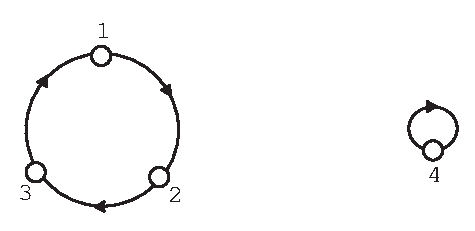
\includegraphics[width=0.73\linewidth]{images/permutationcycledigraph}
\caption{The directed graph of a permutation .\label{permutationcycledigraph}}
\end{figure}
You see that the graph has two directed cycles, the rather trivial one with vertex 4 pointing to itself, and the nontrivial one with vertex 1 pointing to vertex 2 pointing to vertex 3 which points back to vertex 1. A permutation is called a \emph{cycle}\index{cycle (of a permutation)}\index{permutation!cycle of} if its digraph consists of exactly one cycle. Thus \(\begin{pmatrix}1\amp 2\amp 3\cr2\amp 3\amp 1
\end{pmatrix}\) is a cycle but \(\begin{pmatrix}1\amp 2\amp 3\amp 4\cr2\amp 3\amp 1\amp 4
\end{pmatrix}\) is not a cycle by our definition. We write \((1\ 2\ 3)\) or \((2\ 3\ 1)\) or \((3\ 1\ 2)\) to stand for the cycle \(\sigma =\begin{pmatrix}1\amp 2\amp 3\cr2\amp 3\amp 1
\end{pmatrix}\). We can describe cycles in another way as well. A \emph{cycle}\index{cycle of a permutation}\index{permutation!cycle of} of the permutation \(\sigma\) is a list \((i\
\sigma(i)\
\sigma^2(i)
\ \ldots\
\sigma^n(i))\) that does not have repeated elements while the list \((i\ \sigma(i)\
\sigma^2(i)\ \ldots\ \sigma^n(i))\ \sigma^{n+1}(i))\) does have repeated elements. We say that the cycles \((i\
\sigma(i)\
\sigma^2(i)\ \ldots\ \sigma^n(i))\) and \((j\
\sigma(j)\
\sigma^2(j)\ \ldots\ \sigma^n(j))\) are \emph{equivalent} if there is an integer \(k\) such that \(j=
\sigma^k(i)\).%
\begin{activity}[]\label{firstrepeat}
~\par
\begin{enumerate}[label=(\alph*)]
 \item Find the cycles of the permutations \(\rho\), \(\varphi_{1/3}\) and \(\varphi_{12/34}\) in the group \(D_4\).%
\par\medskip\noindent%
\textbf{Solution.}\quad \(\rho\) has one cycle, \((1\ 2\ 3\ 4)\), \(\varphi_{1/3}\) has one cycle \((2\ 4)\), \(\varphi_{12/34}\) has two cycles, namely \((1\ 2)\) and \((3\ 4)\).%

~\par
\item Find the cycles of the permutation \(\begin{pmatrix}1\amp 2\amp 3\amp 4\amp 5\amp 6\amp 7\amp 8\amp 9\cr
3\amp 4\amp 6\amp 2\amp 9\amp 7\amp 1\amp 5\amp 8
\end{pmatrix}\).%
\par\medskip\noindent%
\textbf{Solution.}\quad \(\begin{pmatrix}1\amp 3\amp 6\amp 7
\end{pmatrix}\), \(\begin{pmatrix}2\amp 4
\end{pmatrix}\), and \(\begin{pmatrix}5\amp 9\amp 8
\end{pmatrix}\).%

~\par
\item Show that if \((i\
\sigma(i)\
\sigma^2(i)
\ \ldots\
\sigma^n(i))\) does not have repeated elements while the list \((i\ \sigma(i)\
\sigma^2(i)\ \ldots\ \sigma^n(i))\ \sigma^{n+1}(i))\) does have repeated elements, then \(\sigma^{n+1}(i)=i\), and so all other \(\sigma^s(i)\) are in the cycle.%
\par\medskip\noindent%
\textbf{Solution.}\quad If \(\sigma^{n+1}(i) = \sigma^p(i)\) and \(0\le p\le n\), then \(\sigma^{n+1-p}(i)
=i\), and so the first repeat was not \(\sigma^{n+1}(i)\) after all. Therefore \(\sigma^{n+1}(i)=i\), and acting on \(i\) with succeeding powers of \(\sigma\) just carries us through the list again and again.%

\end{enumerate}
\end{activity}
\begin{activity}[]\label{cyclepartition}
The support set of the cycle \((a_1\ a_2\ \ldots\ a_n)\) is the set \(\{a_1,a_2,\ldots,a_n\}\). Show that the support sets of the cycles of a permutation of the set \(S\) form a partition of \(S\).%
\par\medskip\noindent%
\textbf{Solution.}\quad Every element is in a cycle by the definition of cycles, so suppose two support sets have an element in common. If the cycles are \((i\
\sigma(i)\
\sigma^2(i)\ \ldots\ \sigma^n(i))\) and \((j\
\sigma(j)\
\sigma^2(j)\ \ldots\ \sigma^m(j))\) and \(\sigma^p(i) =\sigma^q(j)\) is a common element, then, \(j=\sigma^{p-q}(i)\). Thus if \(p\ge q\), \(j\) is in the first cycle. Otherwise \(i\) is in the second cycle. If \(j\) is in the first cycle, it is \(\sigma^k(i)\) for some \(i\), and as we take successive powers, we get, by \hyperref[firstrepeat]{Problem~\ref{firstrepeat}} that \(i\) is \(\sigma^h(j)\), and then successive powers of \(\sigma\) just give us the rest of the cycle beginning with \(i\). Therefore the two support sets are identical. A similar argument works if \(i\) is in the second cycle. Thus the support sets partition \(S\).%
\end{activity}
We regard a cycle \((i\
\sigma(i)\
\sigma^2(i)\ \ldots\ \sigma^n(i))\) as standing for the permutation%
\begin{equation*}
\begin{pmatrix}i\amp
\sigma(i)\amp
\cdots\amp \sigma^{n-1}(i)\amp \sigma^n(i)\cr
\sigma(i)\amp
\sigma^2(i)\amp \cdots\amp \sigma^n(i)\amp i
\end{pmatrix} .
\end{equation*}
%
\par
Since interchanging the columns in the two row notation for a permutation does not change the permutation\footnote{Note that not all ways of interchanging the columns list the bottom row in the order of a cycle of \(\sigma\), though.\label{fn-20}}, this means that equivalent cycles represent the same permutation. Thus we consider equivalent cycles to be equal in the same way we consider \({1\over 2}\) and \(2\over 4\) to be equal. In particular, this means that \((i_1\ i_2\
\ldots i_n) = (i_j\ \ i_{j+1}\ \ldots\ i_n\ \ i_1\ \ i_2\ \ldots\ i_{j-1})\).%
\par
If \(\gamma_1\), \(\gamma_2\), \dots{}, \(\gamma_n\) are the (inequivalent) cycles of a permutation \(\sigma\) of the set \(S\), then we write%
\begin{equation*}
\sigma = \gamma_1\gamma_2\cdots\gamma_n= \gamma_{i_1}\gamma_{i_2}
\cdots \gamma_{i_n},
\end{equation*}
that is, we say that \(\sigma\) is the product of its cycles in any order. There are two ways to think of this notation. You can think of it as a brand new kind of multiplication where we multiply a permutation of one set by a permutation of a disjoint set to get a new permutation of the union of the two sets. In this notation \(\sigma(x)\) is determined by which cycle \(\gamma_k\) contains \(x\) in its support set and \(\sigma(x) =
\gamma_k(x)\). You can also think of identifying \(\gamma\) with the product of \(\gamma\) with a collection of one-cycles, one one-cycle for each element of \(S\) not in the support set of \(\gamma\). For example we identify the cycle \((2\  4\ 5)\) in \(S_6\) with \((1)(2\  4\ 5)(3)(6)\). Similarly we identify \((3)\) with \((1)(2)(3)(4)(5)(6)\). But when we use \((3)\) as a notation for \((1)(2)(3)(4)(5)(6)\), we still say its support set is \(\{3\}\). Then the product above is simply composition of functions. We can summarize this discussion with the following theorem\index{disjoint cycles}\index{cycles!disjoint}\footnote{In the statement of the theorem we use the word disjoint; two cycles are said to be \emph{disjoint} if their support sets are disjoint.\label{fn-21}}. The proof of the theorem is essentially your solution to \hyperref[cyclepartition]{Problem~\ref{cyclepartition}}.%
\begin{theorem}[{}]\label{theorem-7}
Every permutation can be written, up to order, in one and only one way as a product of disjoint cycles.%
\end{theorem}
We usually don't bother writing down one-cycles when we write a permutation as a product of cycles; it is a convention to make less work for us. We just have to remember that they are implicitly there. You should recognize that the first interpretation we gave for the multiplication of disjoint cycles applies only when the cycles are disjoint. From now on we will use the phrase ``product of permutations'' to mean the same thing as ``composition of permutations,'' and will use either the notation \(\sigma\circ\varphi\) or \(\sigma\varphi\) for the composition of \(\sigma\) and \(\varphi\), whichever is convenient.%
\begin{activity}[]\label{disjoint-commutative}
~\par
\begin{enumerate}[label=(\alph*)]
 \item Write the permutations \(\rho\), \(\varphi_{1/3}\) and \(\varphi_{12/34}\) in \(D_4\) as products of disjoint cycles.%
\par\medskip\noindent%
\textbf{Solution.}\quad \(\rho = (1\ 2\ 3\ 4)\), \(\varphi_{1/3} = (2\ 4) = (1)(2\ 4)(3)\) (either side of the equation is a right answer), \(\varphi_{12/34} = (1\ 2)(3\        4)\).%

~\par
\item Write the permutation \(\begin{pmatrix}1\amp 2\amp 3\amp 4\amp 5\amp 6\amp 7\amp 8\amp 9\cr
3\amp 4\amp 6\amp 2\amp 9\amp 7\amp 1\amp 5\amp 8
\end{pmatrix}\) as a product of disjoint cycles.%
\par\medskip\noindent%
\textbf{Solution.}\quad \((1\ 3\ 6\ 7)(1\ 4)(5\ 9\ 8)\).%

~\par
\item Explain why, if \(\gamma\) and \(\gamma'\) are two disjoint cycles, then \(\gamma\gamma' =
\gamma'\gamma\).%
\par\medskip\noindent%
\textbf{Solution.}\quad When we compute \(\gamma\gamma'(i)\), the element \(i\) is fixed (i.e. mapped to itself) by either \(\gamma\) or \(\gamma'\). But if \(\gamma'\) fixes \(i\) and \(\gamma(i)=j\), with \(j\not=i\) then \(j\) is in the support set of \(\gamma\), so it is not in the support set of \(\gamma'\). Thus \((\gamma\circ\gamma')(i) =j\). However since \(\gamma'\) fixes \(j\) as well, then \((\gamma'\circ\gamma)(i) =\gamma'(j) =j\) also. If \(\gamma(i)=i\) also, then \(\gamma\gamma'(i) =\gamma'\gamma(i) = i\). A similar argument works if \(\gamma\) fixes \(i\), so in all cases, \(\gamma\gamma'(i) = \gamma'\gamma(i)\), which is what it means to say that \(\gamma\gamma'=\gamma'\gamma\).%

\end{enumerate}
\end{activity}
\begin{activity}[]\label{activity-257}
Write a recurrence for the number \(c(k,n)\) for the number of permutations of \([k]\) that have exactly \(n\) cycles, including 1-cycles. Use it to write a table of \(c(k,n)\) for \(k\) between 1 and 7 inclusive. Can you find a relationship between \(c(k,n)\) and any of the other families of special numbers such as binomial coefficients, Stirling numbers, Lah numbers, etc. we have studied? If you find such a relationship, prove you are right.%
\par\medskip\noindent%
\textbf{Solution.}\quad The element \(k\) is either in a cycle by itself or it isn't. The number of permutations in which it is in a cycle by itself is \(c(k-1,n-1)\). If it is in a cycle with something else, it can come after any of the \(k-1\) elements, and each choice of which one it comes after gives a different permutation. (You can always shift a cycle around so that \(k\) doesn't come first.) Thus \(c(k,n) = c(k-1,n-1) + (k-1)c(k-1,n)\). The table is:%
\begin{tabular}{lllllllll}
\(k/n\)&0&1&2&3&4&5&6&7\tabularnewline[0pt]
&&&&&&&&\tabularnewline\hrulethin
0&1&0&0&0&0&0&0&0\tabularnewline[0pt]
1&0&1&0&0&0&0&0&0\tabularnewline[0pt]
2&0&1&1&0&0&0&0&0\tabularnewline[0pt]
3&0&2&3&1&0&0&0&0\tabularnewline[0pt]
4&0&6&11&6&1&0&0&0\tabularnewline[0pt]
5&0&24&50&35&10&1&0&0\tabularnewline[0pt]
6&0&120&274&225&85&15&1&0\tabularnewline[0pt]
7&0&720&1764&1624&735&175&21&1
\end{tabular}
We see that the table is identical with our earlier table of the Stirling numbers of the first kind, except that in that table there was an alternating pattern of minus signs, offset by one place in successive rows. Thus it must be the case that \(c(k,n)=
|s(k,n)|\). To prove this, note that it is the case when \(k=0\), and also when \(n=1\). Now assume inductively it is true when \(k= m-1\) and notice that if \(n>0\), \(s(m,n)=s(m-1,n-1)-(m-1)s(m-1,n)\), that \(s(m-1,n-1)\) and \(s(m-1,n)\) have opposite signs, so%
\begin{align*}
\hspace{-.5in}|s(m-1)-(m-1)s(m-1,n)|\amp =\amp  |s(m-1| +
(m-1)|s(m-1,n)|\\
\amp =\amp c(m-1,n-1)+(m-1)c(m-1,n)\\
\amp =\amp  c(m,n).
\end{align*}
%
\par
Thus by the principle of mathematical induction \(c(k,n) = |s(k,n)|\) for all nonnegative numbers \(k\) (and all \(n\) between 0 and \(k\).)%
\end{activity}
\begin{activity}[]\label{activity-258}
~\par
\begin{enumerate}[label=(\alph*)]
 \item (Relevant to \hyperref[expogenfun]{Appendix~\ref{expogenfun}}.) A permutation \(\sigma\) is called an \emph{involution}\index{involution} if \(\sigma^2=\iota\). When you write an involution as a product of disjoint cycles, what is special about the cycles?%
\par\medskip\noindent%
\textbf{Solution.}\quad They are all 2-cycles or 1-cycles.%

~\par
\item Write the product \((1\ 2)(1\ 3)(1\ 4)\) in two row notation and then write it in terms of of \emph{disjoint} cycles.%
\par\medskip\noindent%
\textbf{Solution.}\quad \(\begin{pmatrix}1\amp 2\amp 3\amp 4\cr4\amp 1\amp 2\amp 3
\end{pmatrix}\), \((1\ 4\ 3\ 2)\).%

\end{enumerate}
\end{activity}
\typeout{************************************************}
\typeout{Subsection  Signs of permutations and the alternating group}
\typeout{************************************************}
\subsection[{Signs of permutations and the alternating group}]{Signs of permutations and the alternating group}\label{subsection-63}
\begin{activity}[]\label{activity-259}
~\par
\begin{enumerate}[label=(\alph*)]
 \item How many permutations in \(S_n\) may be written as a product of not necessarily disjoint two cycles?%
\par\medskip\noindent%
\textbf{Solution.}\quad All of them, because each cycle can be written as a product on non-disjoint cycles.%

~\par
\item (May be time-consuming.) Consider the permutations of \(\{1,2,3,4\}\) which are \(\iota\) or have one of the forms \((i\ j\ k)\) or \((i\ j)(h\ k)\), where \(i\), \(j\), \(k\), and \(h\) are distinct.  Do these permutations form a subgroup of the group \(S_4\)?  How many of these permutations are there?%
\par\medskip\noindent%
\textbf{Solution.}\quad Note that two cycles in \(S_4\) of the form \((i\ j\ k)\) have two or three elements in common, so they have the same kind of overlap as \((1\ 2\ 3)\) and \((2\ 3\
4)\), \((1\ 2\ 3)\) and \((3\ 2\ 4)\), \((1\ 2\ 3)\) and \((1\ 3\ 2)\), or \((1\ 2\ 3)\) and \((1\
2\ 3)\). The products of these four pairs are, respectively, \((2\ 1)(3\ 4)\), \((2\ 4\
1)\), \((1)(2)(3)= (1)(2)(3)(4)=\iota\), and \((1\ 3\ 2)\). If we take a three-cycle times a product of two two-cycles it will have the same form as \((1\ 2\ 3)(1\ 2)(3\ 4)\) or \((1\ 2\ 3)(1\ 3)(2\ 4)\). The first of these products is \((1\ 3\ 4)\) and the second is \((2\ 4\ 3)\). If we have a product of two elements each of which is a product of two two-cycles, it will have the same form as either \((1\ 2)(3\ 4)(1\ 2)(3\ 4)\) or \((1\ 2)(3\ 4)(1\ 3)(2\ 4)\). The first of these is \(\iota\) and the second is \((1\
4)(2\ 3)\). Thus our set is closed under composition, and so it is a subgroup of \(S_4\). The subgroup has size 12.%

\end{enumerate}
\end{activity}
\begin{activity}[]\label{activity-260}
The \emph{sign} of a 1-cycle, 3-cycle, \dots{}, \((2k-1)\)-cycle is defined to be 1, while the \emph{sign} of a 2-cycle, 4-cycle, \dots{}, \(2k\)-cycle is defined to be -1. The \emph{sign} of a product of disjoint cycles is the product of the signs of its cycles.\index{permutation!sign of}\index{sign of a permutation}%
~\par
\begin{enumerate}[label=(\alph*)]
 \item What happens to the sign of an \(n\)-cycle if you multiply it by a 2-cycle (which might or might not be disjoint from it)?%
\par\medskip\noindent%
\textbf{Solution.}\quad If the \(m\)-cycle and 2-cycle are disjoint, then by definition, the sign changes to the opposite value. If they are not disjoint, and the two cycle is \((i\
j)\), either \(i\) or \(j\) or both are in the original cycle. Suppose that only \(i\) is in the cycle (and the same argument works if only \(j\) is in the cycle), and the original cycle is \((i\ i_2\ \ldots\ i_n)\). Then the product \((i\ i_2\
\ldots\ i_n)(i\ j)\) is \((i\ j\ i_2\ \ldots\ i_n)\), and the product \((i\ j)(i\ i_2\ \ldots\ i_n)\) is \((j\ i\
i_2\
\ldots\ i_n)\). Thus the sign changes to the opposite sign. Suppose that \(i\) and \(j\) are both in the original cycle. Then \(j= i_k\) for some \(k\). Then \((i\ i_2\ \ldots\
i_n)(i\ i_k)=(i i_{k+1}\ i_{k+2}\ \ldots\ i_n)(i_k\ i_2\ \ldots\ i_{k-1})\). If the original sign was 1, then we started with an cycle on an odd number of entries and so now have an cycle on an even number of entries times an cycle on an odd number of entries, so the sign has changed. It the original sign was -1, then we started with an cycle on an even number of entries, so we now have a product of two cycles on an odd number of entries, which gives sign 1, or a product of two cycles on an even number of entries, which gives us sign 1. Thus in every case, the sign changes to the opposite sign.%

~\par
\item What happens to the sign of a product of an \(n\)-cycle and a disjoint \(m\)-cycle if you multiply it by a two cycle which is disjoint from neither of the other two?%
\par\medskip\noindent%
\textbf{Solution.}\quad The product becomes an \(m+n\) cycle, and so if both cycles were on an even number of entries or both were on an odd number, we now have an cycle on an even number of entries, so its sign is -1, but previously the product had sign 1. Thus the sign changes. If one of the original cycles was on an even number of entries and one was on an odd number, we now have a cycle on an odd number of entries, so it has sign 1, while the original product has sign -1. Thus the sign changes.%

~\par
\item What happens to the sign of a permutation if you multiply it by a 2-cycle?%
\par\medskip\noindent%
\textbf{Solution.}\quad The cases we just analyzed cover all the possibilities, so the sign changes.%

~\par
\item A 2-cycle is often called a \emph{transposition}\index{transposition}.  What is the sign of a product of \(k\) (not necessarily disjoint) transpositions? (Don't forget to prove you are correct.)%
\par\medskip\noindent%
\textbf{Solution.}\quad \((-1)^k\). The proof is probably easiest by induction, for the sign of one transposition is -1, and if we take a product of \(i\) transpositions and multiply by one more transposition, the sign changes. Thus if the product of \(i\) transpositions has sign \((-1)^i\), the product of \(i+1\) transpositions has sign \((-1)^{i+1}\), and so by the principle of mathematical induction, the sign of a product of \(k\) transpositions if \((-1)^k\) for all positive integers \(k\). In fact, had we taken \(\iota\) for our base case, we could have concluded the same result for all nonnegative integers.%

~\par
\item Can you compute the sign of a product of two permutations from the signs of the permutations?  Why or why not?%
\par\medskip\noindent%
\textbf{Solution.}\quad You can compute it; it is the product of the signs. Just write them as products of transpositions, multiply all those transpositions together and use the fact that, for transpositions, the sign of the product is the product of the signs.%

\end{enumerate}
\end{activity}
\begin{activity}[]\label{activity-261}
Do the elements of \(S_n\) with sign -1 form a subgroup of \(S_n\)? Do the elements of \(S_n\) with sign 1 form a subgroup of \(S_n\)?%
\par\medskip\noindent%
\textbf{Solution.}\quad The elements of sign \(-1\) are not closed under composition so they do not form a subgroup. The elements of sign \(1\) are closed under composition so they do form a subgroup.%
\end{activity}
\begin{activity}[]\label{alternatinggroup}
Describe a subgroup of \(S_n\) of size \(n!/2\). This subgroup is called the \emph{alternating group}\index{alternating group} \(A_n\). Describe explicitly a partition of \(S_n\) that you can use with the quotient principle to prove bijectively that the subgroup you described has size \(n!/2\).%
\par\medskip\noindent%
\textbf{Solution.}\quad Partition \(S_n\) into the permutations of sign 1 and sign -1. Choose a transposition. Multiplying the elements in one block gives you elements in the other block. Multiplying by the transposition twice gives you the same permutation back, so the function that multiplies by this transposition has an inverse and so is a bijection.%
\end{activity}
\typeout{************************************************}
\typeout{Section 5.2 Groups Acting on Sets}
\typeout{************************************************}
\section[{Groups Acting on Sets}]{Groups Acting on Sets}\label{sec_groups-groupsact}
\typeout{************************************************}
\typeout{Introduction  }
\typeout{************************************************}
We defined the rotation group \(R_4\) and the dihedral group \(D_4\) as groups of permutations of the vertices of a square. These permutations represent rigid motions of the square in the plane and in three dimensional space respectively. The square has geometric features of interest other than its vertices; for example its diagonals, or its edges. Any geometric motion of the square that returns it to its original position takes each diagonal to a possibly different diagonal, and takes each edge to a possibly different edge.%
\par
We could similarly define the group \(R\) of rigid motions of a cube as the group of permutations of its eight vertices that correspond to three dimensional motions that return the cube to its original position, but perhaps with vertices in different places than they were originally. Now each of these motions also takes the 12 edges of the cube to (possibly different) edges and takes the six faces of the cube to (possible different) faces. So we can think of our group \(R\) as acting not only on the vertices of our geometric figure, but on edges, diagonals, faces, or perhaps other geometric features.%
\par
We have seen above that the fact that we have defined a permutation group as the permutations of some specific set doesn't preclude us from thinking of the elements of that group as permuting the elements of some other set as well. In order to keep track of which permutations of which set we are using to define our group and which other set is being permuted as well, we introduce some new language. We are going to say that the group \(D_4\) ``acts'' on the edges and diagonals of a square and the group \(R\) of permutations of the vertices of a cube that arise from rigid motions of the cube ``acts'' on the edges, faces, diagonals, etc. of the cube. Instead of talking about permutations of these edges, faces, etc., we will use an equivalent word and talk about bijections of these objects. In this way it will be easier for us to keep track of which permutations form our original group and how this group relates to other objects of interest.%
\begin{figure}
\centering
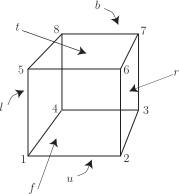
\includegraphics[width=0.5\linewidth]{images/cube1}
\caption{A cube with the positions of its vertices and faces labelled.  The curved arrows point to the positions that are blocked by the cube.\label{cube1}}
\end{figure}
\begin{activity}[]\label{activity-263}
In \hyperref[cube1]{Figure~\ref{cube1}} we show a cube with the positions of its vertices and faces labelled. \emph{Some of the arrows may be missing in this image. Cross check.} As with motions of the square, we let we let \(\varphi(x)\) be the label of the place where vertex previously in position \(x\) is now.%
~\par
\begin{enumerate}[label=(\alph*)]
 \item Write in two row-notation the permutation \(\rho\) of the vertices that corresponds to rotating the cube 90 degrees around a vertical axis through the faces \(t\) (for top) and \(u\) (for underneath).  (Rotate in a right-handed fashion around this axis, meaning that vertex 6 goes to the back and vertex 8 comes to the front.)  Write in two-row notation the bijection \(\beta_{\rho}\) of the faces that corresponds to this member \(\rho\) of \(R\).%
\par\medskip\noindent%
\textbf{Solution.}\quad \(\!\!\!\begin{pmatrix}1\amp 2\amp 3\amp 4\amp 5\amp 6\amp 7\amp 8\cr
2\amp 3\amp 4\amp 1\amp 6\amp 7\amp 8\amp 5
\end{pmatrix}\)~~~~\(\begin{pmatrix}t\amp f\amp r\amp b\amp l\amp u\cr t\amp r\amp b\amp l\amp f\amp u
\end{pmatrix}\)%

~\par
\item Write in two-row notation the permutation \(\varphi\) that rotates the cube 120 degrees around the diagonal from vertex 1 to vertex 7 and carries vertex 8 to vertex 6.  Write in two-row notation the bijection \(\beta_\varphi\) of the faces that corresponds to this member of \(R\).%
\par\medskip\noindent%
\textbf{Solution.}\quad \(\!\!\!\begin{pmatrix}1\amp 2\amp 3\amp 4\amp 5\amp 6\amp 7\amp 8\cr1\amp 4\amp 8\amp 5\amp 2\amp 3\amp 7\amp 6
\end{pmatrix} ~
~\begin{pmatrix}t\amp f\amp r\amp b\amp l\amp u\cr r\amp u\amp b\amp t\amp f\amp l
\end{pmatrix}\)%

~\par
\item Compute the two-row notation for \(\rho\circ\varphi\), for \(\beta_{\rho}\circ\beta_{\varphi}\) (\(\beta_{\rho}\) was defined in \hyperref[actsonparta]{Part~}), and write in two-row notation the bijection \(\beta_{\rho\circ\varphi}\) of the faces that corresponds to the action of the permutation \(\rho\circ\varphi\) on the faces of the cube (for this question it helps to think geometrically about what motion of the cube is carried out by \(\rho\circ\varphi\)).  What do you observe about \(\beta_{\rho\circ\varphi}\) and \(\beta_{\rho}\circ\beta_{\varphi}\)?%
\par\medskip\noindent%
\textbf{Solution.}\quad %
\begin{align*}
\begin{pmatrix}1\amp 2\amp 3\amp 4\amp 5\amp 6\amp 7\amp 8\cr
2\amp 3\amp 4\amp 1\amp 6\amp 7\amp 8\amp 5
\end{pmatrix} \begin{pmatrix}1\amp 2\amp 3\amp 4\amp 5\amp 6\amp 7\amp 8\cr1\amp 4\amp 8\amp 5\amp 2\amp 3\amp 7\amp 6
\end{pmatrix} \amp =\amp
\begin{pmatrix}1\amp 2\amp 3\amp 4\amp 5\amp 6\amp 7\amp 8\cr 2\amp 1\amp 5\amp 6\amp 3\amp 4\amp 8\amp 7
\end{pmatrix} \amp \amp
\end{align*}
%
\begin{align*}
\begin{pmatrix}t\amp f\amp r\amp b\amp l\amp u\cr t\amp r\amp b\amp l\amp f\amp u
\end{pmatrix} \begin{pmatrix}t\amp f\amp r\amp b\amp l\amp u\cr r\amp u\amp b\amp t\amp f\amp l
\end{pmatrix} \amp =\amp
\begin{pmatrix}t\amp f\amp r\amp b\amp l\amp u\cr b\amp u\amp l\amp t\amp r\amp f
\end{pmatrix} \amp \amp
\end{align*}
%
\begin{equation*}
\beta_{\rho\circ\varphi} =\begin{pmatrix}t\amp f\amp r\amp b\amp l\amp u\cr
b\amp u\amp l\amp t\amp r\amp f
\end{pmatrix} =\beta_{\rho}\circ\beta_{\varphi}
\end{equation*}
%

\end{enumerate}
\end{activity}
\begin{activity}[]\label{activity-264}
How many permutations are in the group \(R\)? \(R\) is sometimes called the ``rotation group'' of the cube. Can you justify this?%
\par\medskip\noindent%
\textbf{Solution.}\quad There are eight places where vertex one can go. Once vertex 1 is placed, there are three ways the three edges ``sticking out'' of it can be placed, and then the location of all the vertices is determined. Thus there are 24 elements of the group. Of them, we have the identity, three rotations about each of the three axes through the midpoints of the faces, one additional rotation about each of the six axes joining opposite faces, and \(2\cdot4=8\) additional rotations about each of the four axes joining a vertex to the diagonally (in three dimensions) opposite vertex. This gives us a total of 10+6+8=24 rotations, so every element of the group is a rotation.%
\end{activity}
We say that a permutation group \(G\) \emph{acts}\index{group acting on a set}\index{action of a group on a set} on a set \(S\) if, for each member \(\sigma\) of \(G\) there is a bijection \(\beta_{\sigma}\) of \(S\) such that%
\begin{equation*}
\beta_{\sigma\circ\varphi} = \beta_{\sigma}\circ\beta_{\varphi}
\end{equation*}
for every member \(\sigma\) and \(\varphi\) of \(G\). In \hyperref[cube2]{Problem~} you saw one example of this condition. If we think intuitively of \(\rho\) and \(\varphi\) as motions in space, then following the action of \(\varphi\) by the action of \(\rho\) does give us the action of \(\rho\circ\varphi\). We can also reason directly with the permutations in \(R\) to show that \(R\) acts on the faces of the cube.%
\begin{activity}[]\label{activity-265}
Suppose that \(\sigma\) and \(\varphi\) are permutations in the group \(R\) of rigid motions of the cube. We have argued already that each rigid motion sends a face to a face. Thus \(\sigma\) and \(\varphi\) both send the vertices on one face to the vertices on another face. Let \(\{h,i,j,k\}\) be the set of vertices on a face \(F\).%
~\par
\begin{enumerate}[label=(\alph*)]
 \item What are the vertices of the face \(F'\) that \(F\) is sent to by \(\varphi\)?%
\par\medskip\noindent%
\textbf{Solution.}\quad \(\varphi(h)\), \(\varphi(i)\), \(\varphi(j)\), \(\varphi(k)\).%

~\par
\item What are the vertices of the face \(F''\) that \(F'\) is sent to by \(\sigma\)?%
\par\medskip\noindent%
\textbf{Solution.}\quad \(\sigma(\varphi(h))\), \(\sigma(\varphi(i))\), \(\sigma(\varphi(j))\), \(\sigma(\varphi(k))\).%

~\par
\item What are the vertices of the face \(F'''\) that \(F\) is sent to by \(\sigma\circ\varphi\)?%
\par\medskip\noindent%
\textbf{Solution.}\quad \((\sigma\circ\varphi)(h)=\sigma(\varphi(h))\), \(\sigma(\varphi(i))\), \(\sigma(\varphi(j))\), \(\sigma(\varphi(k))\).%

~\par
\item How have you just shown that the group \(R\) acts on the faces?%
\par\medskip\noindent%
\textbf{Solution.}\quad We have just shown that for each face \(F\), \(\beta_{\sigma\circ\varphi}(F) = \beta_{\sigma} \circ \beta_{\varphi}(F)\), so that \(\beta_{\sigma\circ\varphi} = \beta_{\sigma} \circ
\beta_{\varphi}\).%

\end{enumerate}
\end{activity}
\begin{activity}[]\label{D_4on2-sets}
The group \(D_4\) is a group of permutations of \(\{1,2,3,4\}\) as in \hyperref[dihedral1]{Problem~\ref{dihedral1}}. We are going to show in this problem and in \hyperref[orbits1]{Problem~\ref{orbits1}} how this group acts in a natural way on the two-element subsets of \(\{1,2,3,4\}\). In particular, for each two-element subset \(\{i,j\}\) of \(\{1,2,3,4\}\) and each member \(\sigma\) of \(D_4\) we define \(\beta_{\sigma}(\{i,j\}) = \{\sigma(i),\sigma(j)\}\). Show that with this definition of \(\beta\), the group \(D_4\) acts on the two-element subsets of \(\{1,2,3,4\}\).%
\par\medskip\noindent%
\textbf{Solution.}\quad The action has been defined for us, so all we need to show is that it is indeed an action. We must show that for each permutation \(\sigma\) in \(D_4\), \(\beta_{\sigma}\) is a bijection and in addition we must show that \(\beta_{\sigma}\circ\beta_{\tau}=
\beta_{\sigma\circ\tau}\). If \(\beta_{\sigma}(\{i,j\})=\beta_{\sigma}(\{h,k\})\), then either \(\sigma(i)=\sigma(h)\) and \(\sigma(j)=\sigma(k)\) or else \(\sigma(i)=\sigma(k)\) and \(\sigma(j) =\sigma(h)\). Since \(\sigma\) is a permutation, in the first case we get \(i=h\) and \(j=k\), so that \(\{i,j\}=
\{h,k\}\), and in the second case we get that \(i=k\) and \(j=h\) so that \(\{i,j\} = \{k,h\} =\{h,k\}\). Thus in either case \(\{i,j\} = \{h,k\}\), so that \(\beta_{\sigma}\) a one-to-one function from the finite set of two element subsets of \(\{1,2,3,4\}\) to itself, and so it is a bijection.%
\par
To show that \(\beta_{\sigma}\circ\beta_{\tau} = \beta_{\sigma\circ\tau}\), we note that%
\begin{align*}
(\beta_{\sigma}\circ\beta_{\tau})(\{i,j\}) \amp =\amp
\beta_{\sigma}(\beta_{\tau}(\{i,j\})=\beta_{\sigma}(\{\tau(i).
\tau(j)\})=\\
\sigma({\tau(i),\tau(j)})\amp =\amp \{(\sigma\circ\tau)(i),(\sigma\circ\tau)(j)\} =\\
\amp \amp \beta_{\sigma\circ\tau}(\{i,j\})
\end{align*}
%
\end{activity}
\begin{activity}[]\label{orbits1}
In \hyperref[D_4on2-sets]{Problem~\ref{D_4on2-sets}}, what is the set of two element subsets that you get by computing \(\beta_{\sigma}(\{1,2\})\) for all \(\sigma\) in \(D_4\)? What is the set of two-element subsets you get by computing \(\beta_{\sigma}(\{1,3\})\) for all \(\sigma\) in \(D_4\)? Describe these two sets geometrically in terms of the square.%
\par\medskip\noindent%
\textbf{Solution.}\quad From \(\{1,2\}\) we get \(\{1,2\}\), \(\{2,3\}\), \(\{3,4\}\), and \(\{3,4\}\). From \(\{1,3\}\) we get \(\{1,3\}\) and \(\{2,4\}\). Thus we get the set of edges and the set of diagonals of the square.%
\end{activity}
\begin{activity}[]\label{activity-268}
Using the notation of \hyperref[dihedral3]{Problem~\ref{dihedral3}}, what is the effect of a 180 degree rotation on the diagonals of a square? What is the effect of the flip \(\varphi_{1/3}\) on the diagonals of a square? How many elements of \(D_4\) send each diagonal to itself? How many elements of \(D_4\) interchange the diagonals of a square?%
The 180 degree rotation sends the diagonals to themselves, i.e., it fixes the diagonals. \(\varphi_{1/3}\) fixes the diagonals. So does \(\varphi_{2/4}\) and the identity. However, \(\rho\), \(\rho^3\), \(\varphi_{12/34}\) and \(\varphi_{14/23}\) all exchange the diagonals. Thus four elements fix each diagonal and four elements interchange them.%
\begin{figure}
\centering
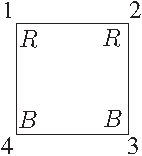
\includegraphics[width=0.2\linewidth]{images/ColoredSquare}
\caption{The colored square corresponding to the function \(f\) with \(f(1) =R\), \(f(2)
= R\), \(f(3)=B\), \(f(4)=B\).\label{ColoredSquare}}
\end{figure}
\end{activity}
\begin{activity}[]\label{actiononfunctions}
Recall that when you were asked in \hyperref[twocolorsofbeads]{Problem~\ref{twocolorsofbeads}} to find the number of ways to place two red beads and two blue beads at the corners of a square free to move in three dimensional space, you were not able to apply the quotient principle to answer the question. This is a simple prototype of the problems we will solve by using permutation groups. Though we don't yet have the tools to solve it, we can get an interesting example of a group acting on a set from it. An assignment of red and blue beads to the corners of a square can be thought of as a function \(f\) from the vertices of the square to the set \(\{R,B\}\). For example, in \hyperref[ColoredSquare]{Figure~\ref{ColoredSquare}} we would have \(f(1) =R\), \(f(2)
= R\), \(f(3)=B\), \(f(4)=B\). What is the original position of the vertex that \(\sigma\) moves to position \(j\)? In terms of \(f\), \(\sigma\) and \(j\), give an expression that represents the color of the vertex in position \(j\) after we apply the permutation \(\sigma\) to the vertices.%
\par\medskip\noindent%
\textbf{Solution.}\quad The original position of the vertex that \(\sigma\) moves to position \(j\) is \(\sigma^{-1}(j)\). Thus the color of the vertex in position \(j\) after we apply \(\sigma\) is \(f(\sigma^{-1}(j))\), which is also \((f\circ
\sigma^{-1})(j)\).%
\end{activity}
\begin{activity}[]\label{actingonfunctions2}
\hyperref[actiononfunctions]{Problem~\ref{actiononfunctions}} suggests that when we have a group of permutations of a set \(S\) and we want to know how it acts on the functions from \(S\) to a set \(C\) (of ``colors''), we should define \(\beta_{\sigma}(f)\) to be \(f\circ\sigma^{-1}\). For the coloring function \(f\) in \hyperref[ColoredSquare]{Figure~\ref{ColoredSquare}}, let \(g=f\circ\rho^{-1}\) and compute \(g(1)\), \(g(2)\), \(g(3)\), and \(g(4)\) so you can see how in this case \(f\circ\rho^{-1}\) is the coloring that results from rotating the colored square by the rotation \(\rho\). Show if a group \(G\) of permutations acts on a set \(S\), then \(\beta_{\sigma}(f) =f\circ\sigma^{-1}\) satisfies the definition of of \(G\) acting on the set of functions \(f\) from \(S\) to \(C\), while \(\beta_{\sigma}(f) =f\circ\sigma\) does not.%
\par\medskip\noindent%
\textbf{Solution.}\quad \(g(1)=B\), \(g(2)=R\), \(g(3)=R\), and \(g(4)=B\).%
\par
If \(\beta_{\sigma}(f) = f\circ\sigma^{-1}\), then%
\begin{align*}
(\beta_{\sigma}\circ\beta_{\tau})(f)\amp =\amp \beta_{\sigma}(\beta_{\tau}(f))\\
\amp =\amp
\beta_{\sigma}(f\circ \tau^{-1})\\
\amp =\amp (f\circ\tau^{-1})\circ\sigma^{-1}\\
\amp =\amp
f\circ(\tau^{-1}\circ \sigma^{-1})\\
\amp =\amp  f\circ (\sigma\circ\tau)^{-1}\\
\amp =\amp \beta_{\sigma\circ\tau}(f).
\end{align*}
%
\par
Therefore \(\beta_{\sigma}(f) = f\circ\sigma^{-1}\) defines an action of a group of permutations of a set \(X\) on functions defined from the set \(X\) to a set \(Y\).%
\par
On the other hand, defining \(\beta_{\sigma}(f) = f\circ\sigma\) does not define a group action. For example, if we consider the function \(f(i)=i\) on the four numbered corners of the square in \hyperref[ColoredSquare]{Figure~\ref{ColoredSquare}}, and take the permutations \(\rho\) and \(\varphi_{1/3}\), we know from the fact that \(f\) is the identity function and \(\rho\) and \(\varphi_{1/3}\) do not commute that \(\beta_{\varphi_{1/3}\circ\rho}(f) = f\circ(\varphi_{1/3}\circ\rho)\not =
f\circ(\rho\circ\varphi_{1/3})=(f\circ\rho)\circ\varphi_{1/3}=\beta_{\rho}(f)
\circ\varphi_{1/3}= \beta_{\varphi_{13}}(\beta_\rho(f)) =(\beta_{\varphi_{1/3}}\circ
\beta_{\rho})(f).\) Thus defining \(\beta_\sigma(f)= f\circ \sigma\) does not give an action of \(D_4\) on functions from the vertices of the square to \(\{1,2,3,4\}\).%
\end{activity}
\begin{activity}[]\label{actingonfunctions3}
If we are interested in something like the number of ways of painting the faces of a cube, and we know how the rotation group of the cube acts on the faces of the cube, then we are interested in how the rotation group acts on functions from the set of faces of the cube to the set of colors. The difference between this problem and \hyperref[actingonfunctions2]{Problem~\ref{actingonfunctions2}} is that in \hyperref[actingonfunctions2]{Problem~\ref{actingonfunctions2}} it was the members \(\sigma\) of our permutation group that were permuting the elements of \(S\), while now we have bijections \(\beta_{\sigma}\) that are permuting the elements of \(S\), in this case the faces of the cube. We want to define a new action \(\beta'_{\sigma}\) of our permutation group on functions from \(S\) to a set \(C\). How should we define \(\beta'_{\sigma}(f)\)? (Hint: think about the example of the faces of the square. After we act on the faces with \(\beta_{\sigma}\), what is the color of the vertex of the cube that is now in position~\(x\)?)%
\par\medskip\noindent%
\textbf{Solution.}\quad We should define \(\beta'_{\sigma}(f) = f\circ
\beta_{\sigma}^{-1}\). The color of the vertex now in position \(x\) is \(f(\beta_{\sigma}^{-1}(x))\) (which is the same as \((f\circ\beta_{\sigma}^{-1})(x)\).%
\end{activity}
\typeout{************************************************}
\typeout{Subsection  Orbits}
\typeout{************************************************}
\subsection[{Orbits}]{Orbits}\label{subsection-64}
In \hyperref[orbits1]{Problem~\ref{orbits1}} you saw that the action of the dihedral group \(D_4\) on two element subsets of \(\{1,2,3,4\}\) seems to split them into two sets, one with two elements and one with 4. We call these two sets the ``orbits'' of \(D_4\) acting on the two elements subsets of \(\{1,2,3,4\}\). More generally, the \emph{orbit}\index{orbit} of a permutation group \(G\) determined by an element \(x\) of a set \(S\) on which \(G\) acts is%
\begin{equation*}
\{\beta_{\sigma}(x)| \sigma \in G\},
\end{equation*}
and is denoted by \(Gx\).%
\par
When we used the quotient principle to count circular seating arrangements or necklaces, we partitioned up a set of lists of people or beads into blocks of equivalent lists. In the case of seating \(n\) people around a round table, what made two lists equivalent was, in retrospect, the action of the rotation group \(R_n\). In the case of stringing \(n\) beads on a string to make a necklace, what made two lists equivalent was the action of the dihedral group. Thus the blocks of our partitions were orbits of the rotation group or the dihedral group, and we were counting the number of orbits of the group action. With this understanding, we will aim to develop tools that allow us to count the number of orbits of a group acting on a set even when the orbits have different sizes. First, though, we have to learn to analyze what the possible sizes of orbits are.%
\begin{figure}
\centering
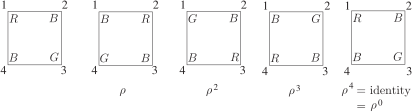
\includegraphics[width=0.95\linewidth]{images/RotationsOfColoredSquare}
\caption{The four possible results of rotating a colored square and maintaining its position.\label{RotationsOfColoredSquare}}
\end{figure}
In \hyperref[RotationsOfColoredSquare]{Figure~\ref{RotationsOfColoredSquare}} we show a square which has had its vertices colored with three colors, and we show how the rotation group \(R_4\) acts on this coloring. If we denote our original coloring by \(f\), then \(g=f\circ\rho^{-1}\) is the function with \(g(1)=B\), \(g(2) = R\), \(g(3)=B\), and \(g(4)=G\). The other functions in the orbit containing \(f\) are shown in \hyperref[RotationsOfColoredSquare]{Figure~\ref{RotationsOfColoredSquare}}.%
\begin{activity}[]\label{dihedralorbits1}
Draw a figure like \hyperref[RotationsOfColoredSquare]{Figure~\ref{RotationsOfColoredSquare}} that illustrates the action of the dihedral group on the function \(f\) above. How many elements are in the orbit of \(f\) under the action of dihedral group? How many elements of the dihedral group fix \(f\); that is, for how many \(\sigma \in D_4\) is \(\beta_{\sigma}(f) =
f\)? How many elements of the dihedral group take \(f\) to \(g\) (where \(g=f\circ
\rho^{-1}\) as earlier)?%
\par\medskip\noindent%
\textbf{Solution.}\quad \leavevmode%
\begin{figure}
\centering
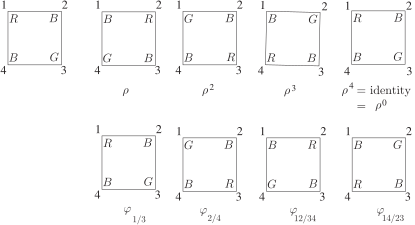
\includegraphics[width=0.95\linewidth]{images/MotionsOfColoredSquare}
\caption{Motions of a colored square\label{MotionsOfColoredSquare}}
\end{figure}
There are four elements in the orbit. Two elements fix \(f\). Two elements take \(f\) to \(g\).%
\end{activity}
\begin{activity}[]\label{dihedralorbits2}
If \(f_1(1)=R\), \(f_1(2) = B\), \(f_1(3) = G\) and \(f_1(4) = G\), how many elements are in the orbit of \(f_1\) under the action of the dihedral group? How many elements of the dihedral group fix \(f_1\); that is, for how many \(\sigma \in D_4\) is \(\beta_{\sigma}(f_1) =
f_1\)? How many elements of the dihedral group take \(f_1\) to \(f_1\circ\rho^{-1}\)?%
\par\medskip\noindent%
\textbf{Solution.}\quad \end{activity}
\begin{activity}[]\label{dihedralorbits3}
If \(f_2(1)=R\), \(f_2(2) = B\), \(f_2(3) = R\) and \(f_2(4) = B\), how many elements are in the orbit of \(f_2\) under the action of the dihedral group? How many elements of the dihedral group fix \(f_2\); that is, for how many \(\sigma \in D_4\) is \(\beta_{\sigma}(f_2) =
f_2\)? How many elements of the dihedral group take \(f_2\) to \(f_2\circ\rho^{-1}\)?%
\par\medskip\noindent%
\textbf{Solution.}\quad \end{activity}
\begin{activity}[]\label{cosets1}
The rotation group of the square with vertices 1, 2, 3, and 4 in \hyperref[cube1]{Figure~\ref{cube1}} can be thought of as a subgroup of the rotation group of the cube. Namely it corresponds to the rotations of the cube around the axis that joins the center of the bottom face with the center of the top face. Recall that we have used \(R\) to stand for the rotation group of the cube. Does \(\beta_{\rho^i}(\sigma)=\rho^i\circ
\sigma\) define an action of \(R_4\) on \(R\)? Does \(\beta_{\rho^i}(\sigma) =
\sigma\circ\rho^i\) define a group action of \(R_4\) on \(R\)? Does \(\beta_{\rho^i}(\sigma) =
\sigma\circ\rho^{-i}\) define a group action of \(R_4\) on \(R\)? For each group action that you found, describe the orbits as simply as you can. How many orbits are there and what are their sizes? (Hint: to do this problem, you don't need to know anything about the rotation group of the cube except for the fact that it is a group that has \(R_4\) as a subgroup and the sizes of \(R_4\) and \(R\) to answer this question.)%
\par\medskip\noindent%
\textbf{Solution.}\quad Yes, \(\beta_{\rho^i}(\sigma)=\rho^i\circ
\sigma\) does define an action of \(R_4\) on \(R\). The orbits are sets of the form \(\{\rho^i\circ\sigma|i=0,1,2,3\}\) for fixed elements \(\sigma\) of \(R\). (For each fixed element \(\sigma\) we get an orbit, but four different elements \(\sigma\) can give the same orbit.) Yes, \(\beta_{\rho^i}(\sigma) =
\sigma\circ\rho^{i}\) does define a group action of \(R_4\) on \(R\). Notice that this gives a group action only because the group \(R_4\) is commutative. The orbits are sets of the form \(\{\sigma\circ\rho^i|i=0,1,2,3\}\) for fixed elements \(\sigma\) of \(R\). Yes, \(\beta_{\rho^i}(\sigma) =
\sigma\circ\rho^{-i}\) does define a group action of \(R_4\) on \(R\). The orbits consist again of sets of the form \(\{\sigma\circ\rho^i|i=0,1,2,3\}\) for fixed elements \(\sigma\) of \(R\). In each case the orbits have size 4 (because if \(\rho^i\circ\sigma=\rho^j\circ\sigma\), then \(\rho^i =\rho^j\), and similarly for \(\sigma\circ\rho^i\)), and there are six of them.%
\end{activity}
\begin{activity}[]\label{activity-276}
What are the sizes of the orbits, and how many have each size, for the action of \(D_6\) on the two element subsets of \(\{1,2,3,4,5,6\}\).%
\par\medskip\noindent%
\textbf{Solution.}\quad There are two orbits of size 6 and one orbit of size 3. (Think of the two-element subsets as the edges and diagonals of a hexagon. The edges form one orbit of size six; the diagonals that jump over two edges form another orbit of size six; and the diagonals connecting opposite vertices form an orbit of size three.%
\end{activity}
\begin{activity}[]\label{coloredhex}
Suppose we draw identical circles at the vertices of a regular hexagon. Suppose we color these circles with two colors, red and blue. We may think of a coloring as a function from the set \(\{1,2,3,4,5,6\}\) to the set \(\{R,B\}\) by numbering the vertices from one to six consecutively around the hexagon. To do this problem it will be helpful to use the notation \(RBRRBB\) to stand for the function \(f\) with \(f(1) =R\), \(f(2)=B\), \(f(3)=R\), \(f(4) = R\), \(f(5)=B\), \(f(6)=B\). How many functions are there from the set \(\{1,2,3,4,5,6\}\) to the set \(\{R,B\}\)? These functions are partitioned into orbits by the action of the rotation group on the hexagon. Using our simplified notation, write down all these orbits and observe what the possible sizes of orbits are.%
\par\medskip\noindent%
\textbf{Solution.}\quad There are 64 functions from a six-element set to a two-element set.%
\par
\(\{RRRRRR\}\),%
\par
\(\{RRRRRB, BRRRRR, RBRRRR, RRBRRR,
RRRBRR, RRRRBR\}\),%
\par
\(\{RRRRBB, BRRRRB, BBRRRR, RBBRRR, RRBBRR, RRRBBR\}\),%
\par
\(\{RRRBRB, BRRRBR, RBRRRB, BRBRRR, RBRBRR, RRBRBR\}\),%
\par
\(\{RRRBBB, BRRRBB, BBRRRB, BBBRRR, RBBBRR, RRBBBR\}\),%
\par
\(\{RRBRRB, BRRBRR, RBRRBR\}\),%
\par
\(\{RRBRBB, BRRBRB, BBRRBR, RBBRRB, BRBBRR, RBRBBR\}\),%
\par
\(\{RRBBRR, RRRBBR, RRRRBB, BRRRRB, BBRRRR, RBBRRR\}\),%
\par
\(\{RRBBRB, BRRBBR, RBRRBB, BRBRRB, BBRBRR, RBBRBR\}\)%
\par
\(\{RRBBBB, BRRBBB, BBRRBB, BBBRRB, BBBBRR, RBBBBR\}\)%
\par
\(\{RBRBRB,
BRBRBR\}\)%
\par
\(\{RBBRBB, BRBBRB, BBRBBR \}\)%
\par
\(\{RBBBBB, BRBBBB, BBRBBB, BBBRBB,BBBBRB, BBBBBR\}\)%
\par
\(\{BBBBBB\}\)%
\par
We have two orbits of size one, one of size two, two of size three, and nine of size six.%
\end{activity}
\begin{activity}[]\label{activity-278}
Either show that, when \(G\) is a group acting on a set \(S\), the orbits of \(G\) partition \(S\) or give a counter-example.%
\par\medskip\noindent%
\textbf{Solution.}\quad Each element \(x\) is in at least one orbit, namely \(Gx\). But if \(x\in Gy\), then \(x=\sigma y\) for some \(\sigma \in G\), so%
\begin{equation*}
Gx=\{\tau x|\tau
\in G\} =
\{\tau\sigma y|\tau\in G\}= \{\tau' y|\tau' \in G\} = Gy.
\end{equation*}
%
\par
Thus each element of \(S\) is in one and only one orbit of \(G\), so the orbits of \(G\) partition \(S\).%
\end{activity}
\begin{activity}[]\label{fixandmove}
In \hyperref[dihedralorbits1]{Problems~\ref{dihedralorbits1}}, \hyperref[dihedralorbits2]{Activity~\ref{dihedralorbits2}}, and \hyperref[dihedralorbits3]{Activity~\ref{dihedralorbits3}}, what set of elements fixes \(f\) and what set of elements takes \(f\) to \(g\), what set of elements fixes \(f_1\) and what set of elements takes \(f_1\) to \(f_1\circ\rho^{-1}\), and what set of elements fixes \(f_2\) and what set of elements takes \(f_2\) to \(f_2\circ\rho^{-1}\)?%
\par\medskip\noindent%
\textbf{Solution.}\quad In \hyperref[dihedralorbits1]{Problem~\ref{dihedralorbits1}}, the set of elements fixing \(f\) is \(\{\iota=\rho^0, \varphi_{1/3}\}\). The set of orbits taking \(f\) to \(g\) is \(\{\rho, \varphi_{12/34}\}\). In \hyperref[dihedralorbits2]{Problem~\ref{dihedralorbits2}} the set of elements fixing \(f_1\) is \(\{\iota\}\), and the set of elements taking \(f_1\) to \(f_1\circ\rho^{-1}\) is \(\{\rho\}\). In \hyperref[dihedralorbits3]{Problem~\ref{dihedralorbits3}}, the set of elements fixing \(f_2\) is \(\{\iota,\rho^2,
\varphi_{1/3}, \varphi_{2/4}\}\), and the set of elements taking \(f_2\) to \(f_2\circ\rho^{-1}\) is \(\{\rho,
\rho^3, \varphi_{12/34}, \varphi_{14/23}\}\).%
\end{activity}
\begin{activity}[]\label{subgroupfixingfunction}
~\par
\begin{enumerate}[label=(\alph*)]
 \item In \hyperref[fixandmove]{Problem~\ref{fixandmove}} the subsets of \(D_4\) that fix a function have a special property. What is it?%
\par\medskip\noindent%
\textbf{Solution.}\quad In each case, the subsets that fix a function form a subgroup. To prove this, note that the subset of group elements fixing a function is closed under composition.%

~\par
\item Could there be a function \(h\) from \(\{1,2,3,4\}\) to the set \(\{R, B,
G\}\) such that the orbit of \(h\) under the action of \(D_4\) has size 3 or 5? If so, find one. If not, explain why not.%
\par\medskip\noindent%
\textbf{Solution.}\quad This is difficult to do at this stage except by ``brute force.'' Here is an organized brute force solution. There is no orbit of size 3 or 5. If a function is constant, then clearly its orbit has size one. If a function has exactly one \(R\) (or \(B\) or \(G\)), then its orbit under the rotations has size 4. Since every flip is a rotation times \(\varphi_{1/3}\), if \(\varphi_{1/3}\) fixes the function, then the orbit has size 4, but if \(\varphi_{1/3}\) does not take the function to the result of a rotation, then neither does a rotation times \(\varphi_{1/3}\), so the orbit has size 8. If the function has exactly three \(R\)'s, then it has exactly one element of some other color, so the argument is the same. If the function has exactly two \(R\)'s and exactly two elements of another color, then if the elements of the same color are adjacent, the orbit under the rotations has size 4, and the result of a flip is the same as the result of a rotation so the orbit has size 4. If the two \(R\)'s are not adjacent, then the orbit under the rotations has size 2 and the result of each flip is the same as the result of a rotation, so the orbit has size 2. If the function has exactly two \(R\)'s, one \(G\), and one \(B\), then the size of the orbit is the same as the orbit in \hyperref[dihedral1]{Problem~\ref{dihedral1}} \hyperref[dihedral3]{or~\ref{dihedral3}}. Any other case is equivalent to one we just covered by changing the names of the colors. Thus there are no orbits of size 3 or 5 (or 6 or 7 either). One can also argue as we will in \hyperref[orbitsize]{Problem~\ref{orbitsize}}.%

\end{enumerate}
\end{activity}
\begin{activity}[]\label{orbitsize}
Make a conjecture about how the size of an orbit of the permutation group \(G\) acting on the set \(S\) relates to the size of \(G\). Prove your conjecture.%
\par\medskip\noindent%
\textbf{Solution.}\quad The size of an orbit divides the size of the group. To prove the conjecture, the most natural approach is to try to use the quotient principle. This requires that we divide the group up into disjoint subsets of the same size. The elements of the group that fix a given element \(x\) form a subgroup \(H\) of \(G\). In each case we have seen, the elements that take \(x\) to \(\sigma(x)\) were of the form \(\sigma\circ\tau\), where \(\tau\) was in the subgroup fixing \(H\). Clearly any such element takes \(x\) to \(\sigma(x)\). The number of such elements is the size of \(H\). And if \(\sigma'(x) = \sigma(x)\), then \(\sigma^{-1}\circ \sigma'\) fixes \(x\) and so is a member \(\tau\) of the subgroup. But then \(\sigma'=\sigma\circ\tau\), where \(\tau=\sigma^{-1}\sigma'\). Thus the number of elements \(\sigma\) that take \(x\) to an element \(\sigma(x)\) is the size of \(H\). And the set of elements that take \(x\) to \(\sigma(x)\) has nothing in common with the set of elements that take \(x\) to \(\sigma_1(x)\), so we have partitioned up the group into subsets each of which has the same size as \(H\), and therefore the size of \(H\) time the number of subsets is the size of \(G\). However the number of subsets is the number of orbits, and so the number of orbits divides the size of the group.%
\end{activity}
\begin{activity}[]\label{sizeofsubgroup}
Make a conjecture about how the size a subgroup of the permutation group \(G\) relates to the size of \(G\).%
\par\medskip\noindent%
\textbf{Solution.}\quad The size of a subgroup of a permutation group \(G\) divides the size of \(G\).%
\end{activity}
\hyperref[alternatinggroup]{Problems~\ref{alternatinggroup}}, \hyperref[cosets1]{Activity~\ref{cosets1}}, \hyperref[fixandmove]{Activity~\ref{fixandmove}} and \hyperref[subgroupfixingfunction]{Activity~\ref{subgroupfixingfunction}} (and less directly \hyperref[actiononfunctions]{Problems~\ref{actiononfunctions}}, \hyperref[actingonfunctions2]{Activity~\ref{actingonfunctions2}} and \hyperref[actingonfunctions3]{Activity~\ref{actingonfunctions3}}) have a common theme.%
\par
In \hyperref[alternatinggroup]{Problem~\ref{alternatinggroup}}, a natural way to show that the group of even permutations, those with sign 1, has size \(n!/2\) is to observe that for any two-cycle (or any odd permutation) \(\tau\), the element \(\sigma\tau\) is odd whenever \(\sigma\) is even and is even whenever \(\sigma\) is odd. Thus if we let \(\tau
A_n\) stand for the set%
\begin{equation*}
\tau A_n = \{\tau\sigma|\sigma \in A_n\},
\end{equation*}
then \(A_n\) and \(tA_n\) are two disjoint sets that partition \(S_n\).%
\begin{activity}[]\label{cosetsize}
Explain why, for any subgroup \(H\) of a permutation group \(G\), \(H\) and \(\tau H\) have the same size.%
\par\medskip\noindent%
\textbf{Solution.}\quad There is a bijection between \(H\) and \(\tau H\) given by \(f(\sigma)
= \tau \sigma\). (It is a bijection because \(\tau\) has an inverse.)%
\end{activity}
By \hyperref[cosetsize]{problem~\ref{cosetsize}} \(A_n\) and \(\tau A_n\) have the same size and since their union has \(n!\) elements, each has size \(n!/2\). The set \(\tau
A_n\) is called a \emph{left coset} of the subgroup \(A_n\) of \(S_n\).%
\par
In \hyperref[cosets1]{Problem~\ref{cosets1}} you probably saw that \(\beta_{\rho^i}(\sigma) =
\rho^i\circ\sigma\) and \(\beta_{\rho^i}(\sigma) = \sigma\circ\rho^{-i}\) both describe actions of \(R_4\) on \(R\). The orbits for the first action are of the form%
\begin{equation*}
R_4\sigma=\{\rho^i \sigma| i=1,2,3,4\},
\end{equation*}
for various elements \(\sigma\) of \(R\). The orbits of the second action are%
\begin{equation*}
\{\sigma r^{-i}| i=1,2,3,4\} = \{\sigma r^i|i = 1,2,3,4\} = \sigma
R_4,
\end{equation*}
for various elements \(\sigma\) of \(R\). The set \(R_4\sigma\) is called a \emph{right coset} of \(R_4\) in \(R\), and as before, the set \(\sigma
R_4\) is called a left coset of \(R_4\) in \(R\). In general when \(H\) is a subgroup of \(G\) and \(\sigma \in G\), we call%
\begin{equation*}
\sigma H = \{\sigma \varphi|\varphi \in H\}
\end{equation*}
a \emph{left coset} of \(H\) in \(G\) and we call%
\begin{equation*}
H\sigma  = \{\varphi\sigma  |\varphi \in H\}
\end{equation*}
a \emph{right coset}\index{coset}\index{left coset}\index{right coset} of \(H\) in \(G\). Notice that \(H\) is a coset of itself, since we may take \(\sigma=\iota\). In \hyperref[cosetsize]{Problem~\ref{cosetsize}} you showed that a subgroup and all its (left) cosets have the same size. Of course the right cosets have that size too.%
\par
When a group \(G\) acts on a set \(S\), we say that an element \(\sigma \in
G\) fixes an element \(x\in S\) if \(\beta_{\sigma}(x) = x\). We say that an element \(\sigma\) takes \(x\) to \(y\) if \(\beta_{\sigma}(x) =y\). In \hyperref[subgroupfixingfunction]{Problem~\ref{subgroupfixingfunction}} the subset of \(D_4\) that fixed \(f\) was a subgroup of \(D_4\), the subset of \(D_4\) fixing \(f_2\) was a subgroup of \(D_4\) and the subset of \(D_4\) fixing \(f_3\) was a subgroup of \(D_4\). The set of group elements that sent \(f\) to \(g\), \(f_2\) to \(f_2\circ\rho^{-1}\) and \(f_3\) to \(f_3\circ\rho^{-1}\) was a coset of the subset that fixed the function in each case.%
\begin{activity}[]\label{cosetspartitionG}
Can two distinct cosets of a subgroup \(H\) of a group \(G\) have an element in common?%
\par\medskip\noindent%
\textbf{Solution.}\quad No, because if \(\tau\in \sigma H\), then \(\tau H =\sigma H\) and if \(\tau \in \varphi H\), then \(\tau H = \varphi H\), so that \(\sigma
H=\varphi H\).%
\end{activity}
\begin{activity}[]\label{activity-285}
Prove your conjecture in \hyperref[sizeofsubgroup]{Problem~\ref{sizeofsubgroup}}.%
\par\medskip\noindent%
\textbf{Solution.}\quad By \hyperref[cosetspartitionG]{Problem~\ref{cosetspartitionG}}, the cosets of a subgroup of \(G\) partition \(G\). But by \hyperref[cosetsize]{problem~\ref{cosetsize}}, the cosets all have the same size, namely the size of \(H\). Thus by the quotient principle, the size of \(H\) is a factor of the size of \(G\).%
\end{activity}
\begin{activity}[]\label{activity-286}
Show that whenever a group \(G\) acts on a set \(S\), then for each \(x\) in \(S\), the set of all elements \(\sigma\) fixing \(x\) is a subgroup of \(G\). We will denote this subgroup by \({ Fix}(x)\).%
\par\medskip\noindent%
\textbf{Solution.}\quad The set of elements fixing \(x\) is closed under composition, and therefore \({ Fix}(x)\) is a subgroup of \(G\).%
\end{activity}
\begin{activity}[]\label{activity-287}
Show that whenever a group \(G\) acts on a set \(S\), then for each \(x\) and \(y\) the set of all \(\tau \in G\) such that \(\beta_{\tau}(x) = y\) is a coset of the subgroup \({ Fix}(x)\) of all elements of \(G\) fixing \(x\).%
\par\medskip\noindent%
\textbf{Solution.}\quad First, if \(\beta_{\tau}(x)=y\) and \(\beta_{\sigma}\) fixes \(x\), then \(\beta_{\tau}\circ \beta_{\sigma}=\beta_{\tau\circ\sigma}\) takes \(x\) to \(y\). Second, if \(\beta_{\varphi}(x)=y\) as well, then \(\beta_{\tau^{-1}}\circ\beta_{\varphi}=\beta_{\tau^{-1}\circ\varphi}\) fixes \(x\) and so is in \({ Fix}(x)\), so that \(\varphi\) is \(\tau\) times an element (namely \(\tau^{-1}\varphi\)) of \({ Fix}(x)\). Thus every element of the coset \(\tau{ Fix}(x)\) takes \(x\) to \(y\), and every element that takes \(x\) to \(y\) is an element of the coset \(\tau{
Fix}(x)\). Thus the set of elements \(\tau\) such that \(\beta_{\tau}(x)=y\) is a coset of \({ Fix}(x)\).%
\end{activity}
\begin{activity}[]\label{activity-288}
When a group \(G\) acts on a set \(S\), how is the number of elements in the orbit containing the element \(x\) of \(S\) related to the size of \(G\) and the size of \({ Fix}(x)\)? Find a bijection that proves that what you say is correct.%
\par\medskip\noindent%
\textbf{Solution.}\quad The number of elements in the orbit containing the element \(x\) is the number of cosets of \({ Fix}(x)\), which is also \(|G|/|{ Fix}(x)|\). A bijection that proves this is the function \(f\) that takes the coset \(\varphi{ Fix}(x)\) to the element \(\varphi(x)\). This function is well-defined because all the elements in \(\varphi{
Fix}(x)\) take \(x\) to \(\varphi(x)\). It is onto because if \(\tau(x) =y\), then the coset \(\tau{ Fix}(x)\) is mapped to \(y\). It is one-to-one because if \(f(\varphi{ Fix}(x))=f(\tau{ Fix}(x))\), then \(\varphi\in \tau{ Fix}(x)\) and \(\tau \in \varphi{ Fix}(x)\), which means the two cosets are identical. The cosets all have the same size, namely \(|{ Fix}(x)|\) and therefore by the quotient principle, the number of cosets is \(|G|/|{ Fix}(x)|\).%
\end{activity}
We can summarize our findings in this section with a theorem.%
\begin{theorem}[{}]\label{theorem-8}
When a group \(G\) acts on a set, the set \({ Fix}(x)\) of group elements fixing any given any given element \(x\) of \(S\) is a subgroup of \(G\). The set of group elements \(\tau\) such that \(\beta_{\tau}(x) = y\) is a coset of \({ Fix}(x)\), and the size of the orbit of \(x\) under the action of \(G\) is \(|G|/|{ Fix}(x)|\).%
\end{theorem}
\typeout{************************************************}
\typeout{Subsection  Multiorbits}
\typeout{************************************************}
\subsection[{Multiorbits}]{Multiorbits}\label{subsection-65}
\begin{activity}[]\label{multiorbits1}
Draw figures like \hyperref[RotationsOfColoredSquare]{Figure~\ref{RotationsOfColoredSquare}} to show the eight results of acting with the dihedral group on the squares corresponding to the functions \(f\), \(f_1\), and \(f_2\) of \hyperref[dihedralorbits1]{Problems~\ref{dihedralorbits1}}, \hyperref[dihedralorbits2]{Activity~\ref{dihedralorbits2}}, and \hyperref[dihedralorbits3]{Activity~\ref{dihedralorbits3}}.%
\par\medskip\noindent%
\textbf{Solution.}\quad \leavevmode%
\begin{figure}
\centering
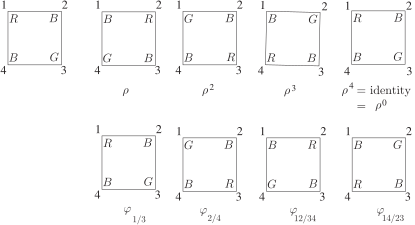
\includegraphics[width=0.95\linewidth]{images/MotionsOfColoredSquare}
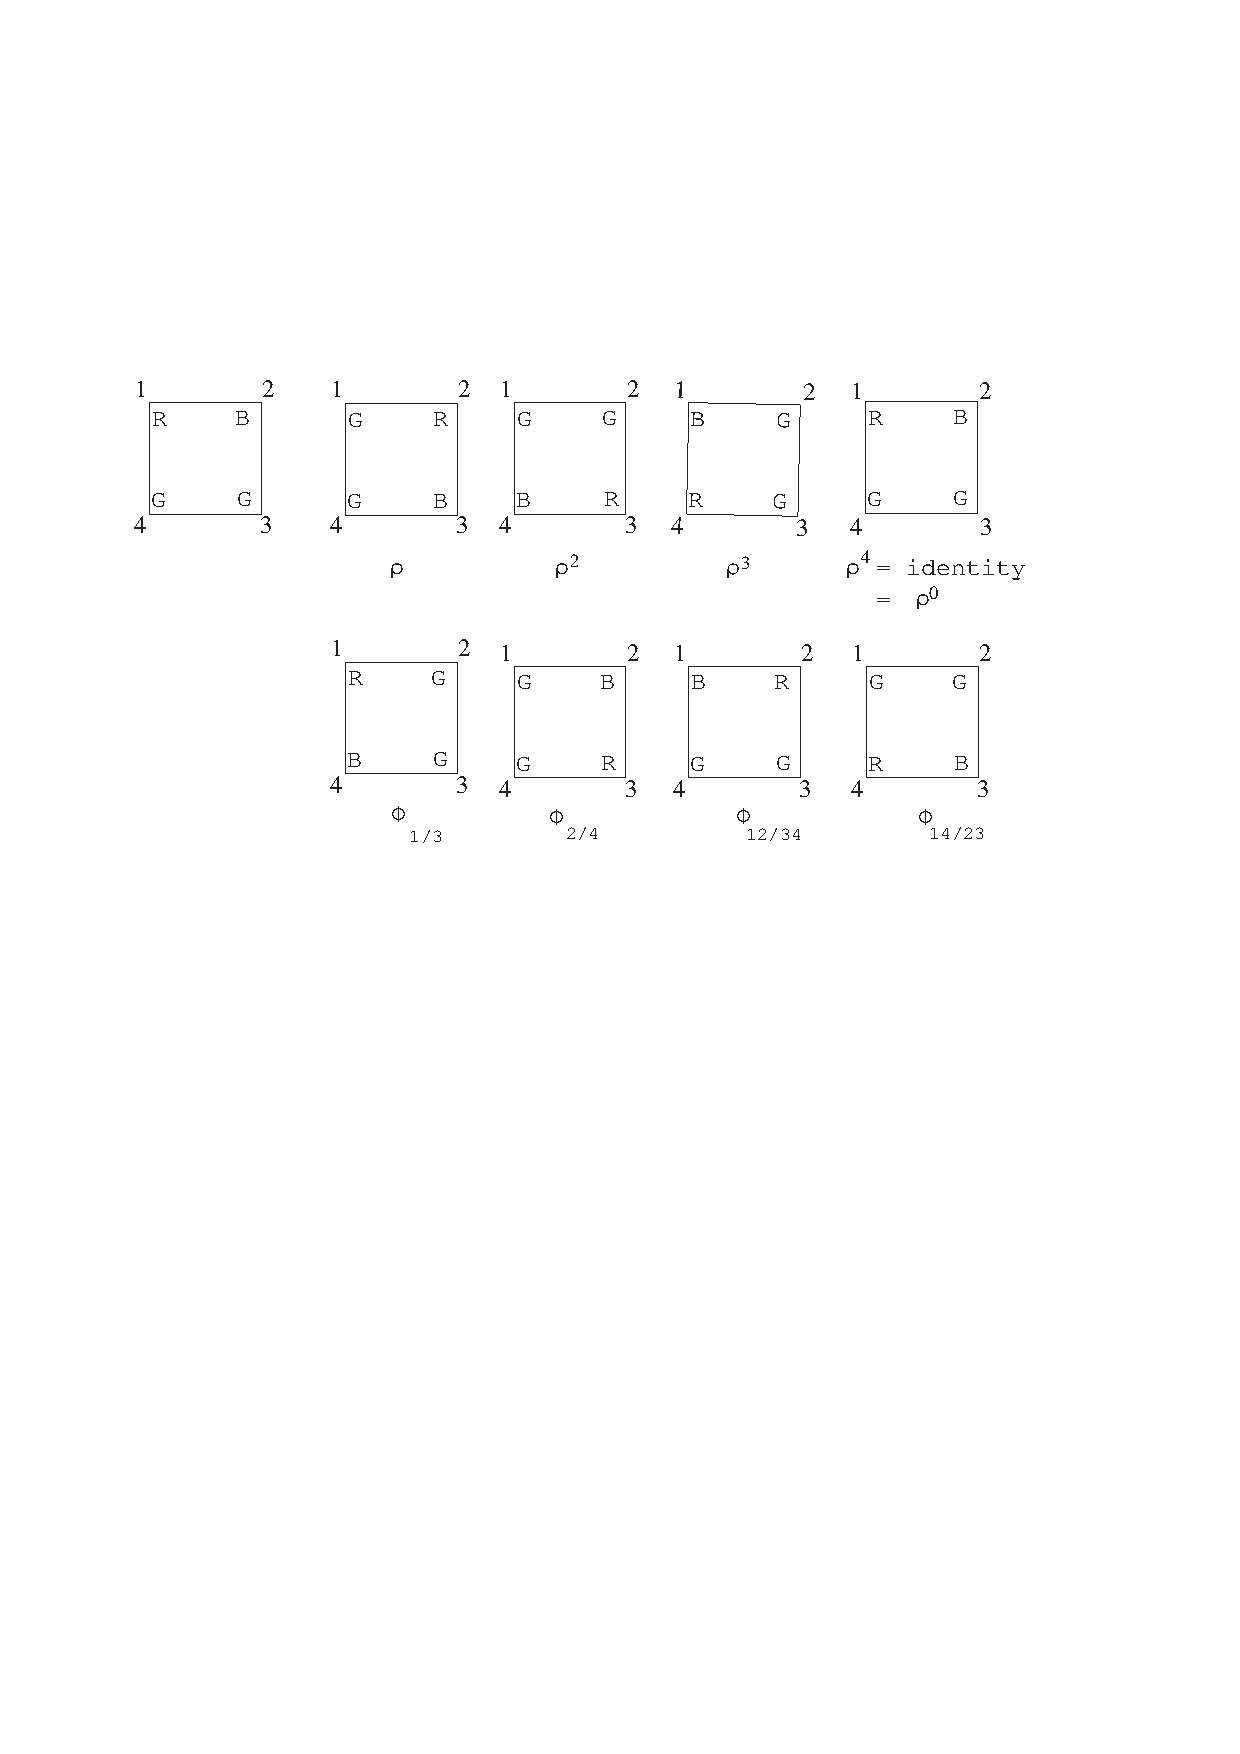
\includegraphics[width=0.95\linewidth]{images/MotionsOfColoredSquare1}
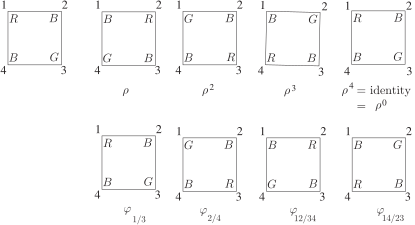
\includegraphics[width=0.95\linewidth]{images/MotionsOfColoredSquare}
\end{figure}
\end{activity}
As \hyperref[multiorbits1]{Problem~\ref{multiorbits1}} shows, in some ways it is more natural to think of an orbit as a multiset rather than a set. For example with the function \(f_2\) from \hyperref[dihedralorbits3]{Problem~\ref{dihedralorbits3}} we get \(f_2\) itself four times when we act with the dihedral group and we get \(f_2\circ\rho^{-1}\) four times when we act on \(f_2\) with the dihedral group. If we think only about the orbit of the dihedral group, then, we lose some information. To avoid this, we define the \emph{multiorbit} of an element \(x\) of a set \(S\) under the action of a group \(G\) to be the multiset%
\begin{equation*}
Gx_{\mbox{\scriptsize multi} } = \{\beta_{\sigma}(x)|\sigma \in
G\}_{\mbox{\scriptsize multi} }.
\end{equation*}
%
\par
It is immediate that the size of each multiorbit is then exactly the size of \(G\).%
\begin{activity}[]\label{NumberContainingx}
In how many different multiorbits of the action of \(G\) on \(S\) will a given element of \(S\) appear?%
\par\medskip\noindent%
\textbf{Solution.}\quad Only one, because the orbits partition \(S\), and there is a bijection between the orbits and the multiorbits given by \(f(Gx) =
Gx_{\mbox{\scriptsize multi} }\).%
\end{activity}
\begin{activity}[]\label{activity-291}
What will the multiplicity of \(x\) be in \(Gx_{\mbox{\scriptsize multi} }\)?%
\par\medskip\noindent%
\textbf{Solution.}\quad \(|{ Fix}(x)|\).%
\end{activity}
It is also immediate from \hyperref[NumberContainingx]{Problem~\ref{NumberContainingx}} that the number of orbits is the number of multiorbits, because we get the orbits from the multiorbits by deleting repeated elements, and the problem shows that each orbit corresponds to exactly one multiorbit\footnote{You might want to argue that we have a multiset of multiorbits, one for each element of \(S\), but that would defeat our purpose since we have  bijection between the set of orbits and the \emph{set} of multiorbits, and this bijection will let us count the number of orbits by computing the size of the set of multiorbits.\label{fn-22}}. We define the union of multisets \(M_1\), \(M_2\), \dots{}, \(M_n\) to be the multiset in which the multiplicity of an element \(x\) is the sum of its multiplicities in the individual multisets \(M_i\). Thus%
\begin{equation*}
\{a,a,b,b,b\}\cup \{a,b,b,c,c,c\}=\{a,a,a,b,b,b,b,b,c,c,c\}.
\end{equation*}
%
\par
We will now get a formula for the number of multiorbits by using the fact that they all have the same size and the idea of multiset union.%
\begin{activity}[]\label{numbermultiorbits1}
How does the size of the union of the set of multiorbits of a group \(G\) acting on a set \(S\) relate to the number of multiorbits and the size of \(G\)?%
\par\medskip\noindent%
\textbf{Solution.}\quad It is simply the product of the number of multiorbits and the size of \(G\).%
\end{activity}
\begin{activity}[]\label{numbermultiorbits2}
How does the size of the union of the set of multiorbits of a group \(G\) acting on a set \(S\) relate to the numbers \(|{
Fix}(x)|\)?%
\par\medskip\noindent%
\textbf{Solution.}\quad Since it is the sum of the multiplicities of the elements of \(S\) in the union, it is the sum of \(|{ Fix}(x)|\) over all \(x\) in \(S\).%
\end{activity}
\begin{activity}[]\label{numbermultiorbits3}
In \hyperref[numbermultiorbits1]{Problems~\ref{numbermultiorbits1}} and \hyperref[numbermultiorbits2]{Activity~\ref{numbermultiorbits2}} you computed the size of the union of the set of multiorbits of a group \(G\) acting on a set \(S\) in two different ways, getting two different expressions which must be equal. Write the equation that says they are equal and solve for the number of multiorbits, and therefore the number of orbits.%
\par\medskip\noindent%
\textbf{Solution.}\quad Using \(m\) for the number of multiorbits, we get%
\begin{equation*}
m|G|=\sum_{x:x\in S} |{ Fix}(x).
\end{equation*}
%
\par
Therefore,%
\begin{equation*}
m={1\over
|G|}\sum_{x:x\in S} |{ Fix}(x)|.
\end{equation*}
%
\end{activity}
\typeout{************************************************}
\typeout{Subsection  The Cauchy-Frobenius-Burnside Theorem}
\typeout{************************************************}
\subsection[{The Cauchy-Frobenius-Burnside Theorem}]{The Cauchy-Frobenius-Burnside Theorem}\label{subsection-66}
\begin{activity}[]\label{numbermultiorbits4}
In \hyperref[numbermultiorbits3]{Problem~\ref{numbermultiorbits3}} you stated and proved a theorem that expresses the number of orbits in terms of the number of group elements fixing each element of \(S\). It is often easier to find the number of elements fixed by a given group element than to find the number of group elements fixing an element of \(S\). For this purpose,%
~\par
\begin{enumerate}[label=(\alph*)]
 \item Let \(\chi(\sigma,x)=1\) if \(\sigma(x)=x\) and let \(\chi(\sigma,x) =0\) otherwise.  Use \(\chi\) to convert the single summation in \hyperref[numbermultiorbits3]{Problem~\ref{numbermultiorbits3}} into a double summation over elements \(x\) of \(S\) and elements \(\sigma\) of \(G\).%
\par\medskip\noindent%
\textbf{Solution.}\quad %
\begin{equation*}
m={1\over |G|}\sum_{x:x\in S}\sum_{\sigma:\sigma\in G}
\chi(\sigma,x).
\end{equation*}

~\par
\item Reverse the order of the previous summation in order to convert it into a single sum involving the function \(\chi\) given by\footnote{The reason for using the Greek letter \(\chi\) is that \(\chi(\sigma)\) is an example of what is called a group character.  Character theory is a major ingredient of the representation theory of groups, an advanced subject that combines abstract beauty with amazing utility.\label{fn-23}}%
\begin{equation*}
\chi(\sigma) =
\mbox{the number of elements of \(S\) left fixed by \(\sigma\)} .
\end{equation*}
%
\par\medskip\noindent%
\textbf{Solution.}\quad %
\begin{equation*}
m={1\over |G|}\sum_{\sigma:\sigma \in G} \chi(\sigma).
\end{equation*}

\end{enumerate}
\end{activity}
In \hyperref[numbermultiorbits4]{Problem~\ref{numbermultiorbits4}} you gave a formula for the number of orbits of a group \(G\) acting on a set \(X\). This formula was first worked out by Cauchy in the case of the symmetric group, and then for more general groups by Frobenius. In his pioneering book on Group Theory, Burnside used this result as a lemma, and while he attributed the result to Cauchy and Frobenius in the first edition of his book, in later editions, he did not. Later on, other mathematicians who used his book named the result ``Burnside's Lemma,"\index{Burnside's Lemma} which is the name by which it is still most commonly known. Let us agree to call this result the Cauchy-Frobenius-Burnside Theorem,\index{Cauchy-Frobenius-Burnside Theorem} or CFB Theorem for short in a compromise between historical accuracy and common usage.%
\begin{activity}[]\label{activity-296}
In how many ways may we string four (identical) red, six (identical) blue, and seven (identical) green beads on a necklace?%
\par\medskip\noindent%
\textbf{Solution.}\quad We are stringing 17 beads on our necklace, so we are asking for the number of orbits of the group \(D_{17}\) on lists of four \(R\)s, six \(B\)s, and seven \(G\)s. For a rotation \(\rho^i\) to fix a list, it must take an \(R\) to a \(R\). The powers of \(\rho^i\) form a group. Thus the set of places that contain an \(R\) in a list that is fixed by \(\rho^i\) must be an orbit of that group. But the size of the orbit must be a divisor of the size of the subgroup, which must be a divisor of seventeen, so the size of the orbit is one or 17. If it is 1, then \(i=0\). Thus no elements are fixed by any nontrivial rotation, and all \(\binom{17}{4,6,7}\) lists of \(R\)s, \(B\)s and \(G\)s are fixed by the identity. Each flip will be a flip \strut around a line from a bead to the spot between the two ``opposite'' beads. This line divides the list into the eight beads on its left, the eight beads on its right and the one bead it goes through. If a flip fixes a list, the eight beads on the left must be identical to the eight beads on the right, meaning that the bead the line goes through must be one of the seven green beads. Thus the number of lists that are fixed by a flip is the number of ways to place three green beads, two red beads, and three blue beads in 8 slots, which is \(\binom{8}{3,2,3}\), or \(8!\over3!2!3!\). There are 17 flips, so there are \(17\cdot8!\over3!2!3!\) elements fixed by flips. Therefore we have%
\begin{equation*}
{1\over
2\cdot 17}\left({17!\over 4!6!7!} + {17\cdot8!\over 3!2!2!}\right) =
{8\cdot15!\over 4!6!7!} + {4\cdot7!\over 3!2!3!}= 120,400
\end{equation*}
necklaces. The numerical answer, which is unimportant here, was obtained from Maple.%
\end{activity}
\begin{activity}[]\label{activity-297}
If we have an unlimited supply of identical red beads and identical blue beads, in how many ways may we string 17 of them on a necklace?%
\par\medskip\noindent%
\textbf{Solution.}\quad We are asking for the number of orbits of \(D_{17}\) on the set of functions from \([17]\) to \(\{R,B\}\). Every function is fixed by the identity. The only functions fixed by a nontrivial rotation are the constant functions. Each flip is around a line from a bead to the space between the two ``opposite'' beads. The bead the line goes through can be either color, and then the eight beads to the left of this one must be identical to the eight beads to the right of this one. There are \(2^8\) ways to assign beads to the positions on the left, so a flip fixes \(2^9\) functions. Therefore by the CFB theorem, we have%
\begin{equation*}
{1\over 2\cdot 17}\left(2^{17}+ 17\cdot2^9+16\cdot 2\right)={2^{16}\over
17}+2^8 +{2^4\over 17}=16{4097\over17}+256=4112
\end{equation*}
necklaces.%
\end{activity}
\begin{activity}[]\label{activity-298}
If we have five (identical) red, five (identical) blue, and five (identical) green beads, in how many ways may we string them on a necklace?%
\par\medskip\noindent%
\textbf{Solution.}\quad Here we need to consider the action of \(D_{15}\) on lists (functions from \([15]\) to \(\{R,B,G\}\)) with five \(R\)s, five \(B\)s, and five \(G\)s. The identity will fix \(\binom{15}{5,5,5}\) lists. A rotation through 3,6,9,or 12 places will fix any function that has the same value in places 1, 4, 7, 10, and 13, the same value in places 2, 5, 8, 11, and 14, and the same value in places 3, 6, 9, 12, and 15. There are \(3!\) such lists. There is no other rotation that fixes any lists. Each flip is around an axis that goes from bead to the space between two opposite beads. If it fixed a list, the seven colors to the left of the axis would have to equal the seven colors to the right of the axis. Thus the number of beads of each color on the left and right sides would have to be equal. So except for the color of the bead the axis goes through, we would have to have an even number of beads of each color for a flip to fix a list of beads. Thus no flip fixes any functions. Therefore by the CFB theorem we have%
\begin{equation*}
{1\over2\cdot15}\left({15!\over5!5!5!} +4\cdot 3!\right)=25,226
\end{equation*}
necklaces. (The numerical answer, which was obtained from Maple, is not important here.)%
\end{activity}
\begin{activity}[]\label{activity-299}
~\par
\begin{enumerate}[label=(\alph*)]
 \item In how many ways may we paint the faces of a cube with six different colors, using all six?%
\par\medskip\noindent%
\textbf{Solution.}\quad Here we must consider the action of the rotation group of the cube on lists of six distinct colors. But no nontrivial rotation will fix a cube with all its faces colored differently. The identity rotation will fix all \(6!\) lists, and there are 24 members of the rotation group, so we have \(6!/24=6\cdot5=30\) ways to paint the faces of a cube with six distinct colors, using each color%

~\par
\item In how many ways may we paint the faces of a cube with two colors of paint? What if both colors must be used?%
\par\medskip\noindent%
\textbf{Solution.}\quad We must consider the action of the rotation group of the cube on functions from \([6]\) to \(\{R,B\}\) or some other two-element set of colors. There are five kinds of elements in the rotation group of the cube. There is one identity, there are six rotations by 90 degrees or 270 degrees around an axis connecting the centers of two opposite faces, there are three rotations of 180 degrees around such an axis, there are 8 rotations (of 120 degrees and 240 degrees, respectively) around an axis connecting two diagonally opposite vertices, and there are 6 rotations of 180 degrees around an axis connecting the centers of two opposite edges. The identity fixes \(2^6\) functions. There are eight functions fixed by a 90 degree or 270 degree rotation. There are 16 functions fixed by a 180 degree rotation along an axis through two faces. There are 8 functions fixed by a 180 degree rotation along an axis joining the centers of two opposite sides. There are 4 functions fixed by a 120 degree or 240 degree rotation. Thus by the CFB theorem, we have%
\begin{equation*}
{1\over24}(64+6\cdot8 + 3\cdot16+ 8\cdot 4 +6\cdot8)= 10
\end{equation*}
ways to paint the faces of a cube with two colors of paint. Two of these colorings use only one color, so there are eight colorings that use both colors.%

\end{enumerate}
\end{activity}
\begin{activity}[]\label{Catalancircle}
In how many ways may we color the edges of a (regular) \((2n+1)\)-gon free to move around in the \emph{plane} (so it cannot be flipped) if we use red \(n\) times and blue \(n+1\) times? If this is a number you have seen before, identify it. \index{Catalan Number!(\hyperref[Catalancircle]{Problem~\ref{Catalancircle}})}%
\par\medskip\noindent%
\textbf{Solution.}\quad The set of all powers of a rotation is a subgroup of the rotation group of the \((2n+1)\)-gon. If a given rotation fixes a coloring, all powers of that rotation fix the coloring. The set of edges to which a given edge is taken by that rotation is an orbit of the group of powers of the rotation. The size of this orbit is a divisor of the size of the subgroup, which is a divisor of \(2n+1\). If the edge is colored red, the size of the orbit is also a divisor of \(n\), and if the edge is colored blue, the size of the orbit is also a divisor of \(n+1\). But neither \(n\) nor \(n+1\) have common divisors with \(2n+1\), except for one. Therefore the only rotation that fixes a coloring is the identity rotation, and it fixes all \(\binom{2n+1}{n}\) colorings. Thus the number of orbits is%
\begin{equation*}
{1\over 2n+1}\binom{2n+1 }{n} = {1\over n+1}\binom{2n}{n},
\end{equation*}
a Catalan number.%
\end{activity}
\begin{activity}[]\label{activity-301}
In how many ways may we color the edges of a (regular) \((2n+1)\)-gon free to move in \emph{three-dimensional space} so that \(n\) edges are colored red and \(n+1\) edges are colored blue. Hint: your answer may depend on whether \(n\) is even or odd.%
\par\medskip\noindent%
\textbf{Solution.}\quad The set of all powers of a rotation is a subgroup of the dihedral group of the \((2n+1)\)-gon. If a given rotation fixes a coloring, all powers of that rotation fix the coloring. The set of edges to which a given edge is taken by that rotation is an orbit of the group of powers of the rotation. The size of this orbit is a divisor of the size of the subgroup, which is a divisor of \(2n+1\). If the edge is colored red, the size of the orbit is also a divisor of \(n\), and if the edge is colored blue, the size of the orbit is also a divisor of \(n+1\). But neither \(n\) nor \(n+1\) have common divisors with \(2n+1\), except for one. Therefore the only rotation that fixes a coloring is the identity rotation, and it fixes all \(\binom{2n+1}{n}\) colorings.%
\par
A flip, on the other hand can fix some colorings. In particular, if \(n\) is even, we color one edge blue, leaving an even number \(n\) of edges to be colored blue and an even number \(n\) of edges to be colored red. It the flip over the axis perpendicular to the side we picked fixes the coloring, the \(n\) edges to the right of the chosen edge must be colored identically with the \(n\) edges to the left of the chosen edge. There are \(\binom{n}{n/2}\) ways to color the \(n\) edges to the right of the chosen edge (choose which edges get red), and so this is the number of colorings fixed by this flip. We have \(2n+1\) flips, and since we have one flip of the type described for each edge, all flips have the form given above. Thus each flip fixes \(\binom{n}{n/2}\) colorings.%
\par
Thus the number of orbits is%
\begin{equation*}
{1\over 2(2n+1)}\left(\binom{2n+1}{n} +
(2n+1)\binom{n}{n/2}\right).
\end{equation*}
%
\par
If \(n\) is odd, we color one edge red, leaving an even number \(n-1\) of edges to be colored red and an even number \(n+1\) of edges to be colored blue. With an argument similar to the previous one we see that there are%
\begin{equation*}
{1\over 2(2n+1)}\left(\binom{2n+1}{n} + (2n+1)(\binom{n}{(n-1)/2}\right)
\end{equation*}
orbits.%
\end{activity}
\begin{activity}[]\label{activity-302}
(Not unusually hard for someone who has worked on chromatic polynomials.) How many different proper colorings with four colors are there of the vertices of a graph which is cycle on five vertices? (If we get one coloring by rotating or flipping another one, they aren't really different.)%
\par\medskip\noindent%
\textbf{Solution.}\quad We are asking for the number of orbits of \(D_5\) on lists of five colors chosen from the given four with no two adjacent colors equal; we consider the first and last position adjacent as well. The identity fixes all such colorings. For those who are familiar with the chromatic polynomial, as in \hyperref[chrompolydel_cont]{Problem~\ref{chrompolydel_cont}}, the number of such colorings is the chromatic polynomial of the cycle on five vertices evaluated at 4. The number of ways to properly color a cycle on five vertices is the number of ways to color a path on five vertices minus the number of ways to color a path on five vertices so that its first and last vertices are identical, which is the number of ways to color a cycle on four vertices. The number of ways to color a cycle on four vertices is the number of ways to color a path on four vertices minus the number of ways to color a path on four vertices so that the first and last vertices are the same color, which is the same as the number of ways to color a cycle on three vertices. The number of ways to properly color a path on five vertices with four colors is \(4\cdot3^4\). The number of ways to properly color a path on four vertices with four colors is \(4\cdot3^3\). The number ways to properly color a cycle on three vertices with four colors is \(4\cdot3\cdot2\). Thus the number of proper colorings of a five vertex cycle with four colors is \(4\cdot3^4-4\cdot3^3
+4\cdot3\cdot2=240\). This is the number of colorings fixed by the identity. No proper coloring is fixed by a nontrivial rotation, because if a rotation of the five cycle fixes a coloring, all the vertices must have the same color. No proper coloring is fixed by a flip, because for a flip to fix a coloring, the coloring must give the same color to two adjacent vertices. Thus the number of really different proper four-colorings of a cycle on 5 vertices is \({240\over 10}=24\).%
\end{activity}
\begin{activity}[]\label{activity-303}
How many different proper colorings with four colors are there of the graph in \hyperref[starhexagon]{Figure~\ref{starhexagon}}? Two graphs are the same if we can redraw one of the graphs, not changing the vertex set or edge set, so that it is identical to the other one. This is equivalent to permuting the vertices in some way so that when we apply the permutation to the endpoints of the edges to get a new edge set, the new edge set is equal to the old one. Such a permutation is called an \emph{automorphism}\index{automorphism (of a graph)} of the graph. Thus two colorings are different if there is no automorphism of the graph that carries one to the other one.%
\begin{figure}
\centering
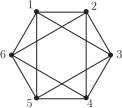
\includegraphics[width=0.33\linewidth]{images/NumberedHexagonalNetwork}
\caption{A graph on six vertices.\label{starhexagon}}
\end{figure}
\par\medskip\noindent%
\textbf{Solution.}\quad We want the number of orbits of the set of proper colorings under the action of the group of automorphisms of the graph. An automorphism \(\sigma\) maps vertex 1 to any of six vertices. Vertex 2 can be mapped to any of the four vertices adjacent to the image of vertex 1. Vertex 3 is adjacent to vertices 1 and 2, so it must be mapped to a vertex adjacent to the images of both vertex 1 and vertex 2; by checking cases you can see that there are always exactly two vertices adjacent to the images of vertex 1 and vertex 2, and mapping vertex 3 to either of these vertices preserves all the edges among vertices 1, 2, and 3. However each of the other three vertices is adjacent to exactly two vertices of the set \(\{1,2,3\}\), and thus it must be mapped to the unique vertex adjacent to the corresponding two of \(\sigma(1)\), \(\sigma(2)\) and \(\sigma(3)\). (It is always the case that each vertex is adjacent to exactly two of these, as you can see by considering the cases with \(\sigma(1)=1\).) Thus there are \(6\cdot4\cdot2=48\) elements in the group. Now to apply the CFB theorem we would need to know how many proper colorings are fixed by each group element, so we would need to know what the group elements are. We have observed that a permutation that preserves the edges is determined by where the triangle \(\{1,2,3\}\) goes. We can see eight triangles in the graph, triangles of the form \(\{i,i+1,i+2\}\), where we identify 7 with 1 and 8 with 2, and the triangles \(\{1,3,5\}\) and \(\{2,4,6\}\). We can map the set \(\{1,2,3\}\) to any of these eight sets by six one-to-one maps, so each group element is determined uniquely by one of these mappings. However focusing on these triangles makes our job here simpler in another way. In a proper coloring, vertices 1, 2, and 3 must be colored differently. We have four choices for the color of vertex 1, three different ones for vertex 2 and two still different ones for vertex 3, so there are 24 ways to color this triangle. Clearly the only difference among these ways is the actual names of the colors. That is, we can assume that vertex 1 is colored red, vertex 2 is colored blue and vertex 3 is colored green, then determine the proper colorings starting with these three colors, and up to changing the names of the colors, we will have determined all the proper colorings. Then we can ask which group elements fix a coloring rather than which colorings are fixed by a group element. This turns out to be easier. Let us write \(RBGRBG\) for the coloring that colors vertices 1 and 4 red, two and five blue, and three and six green. An examination of the figure shows that this is a proper coloring. In fact, it is the only proper coloring that starts \(RBG\) and uses only three colors. Suppose we were to use a fourth color, \(Y\). Then among vertices 4, 5, and 6, it could be used in just one place, because those three vertices are mutually adjacent. Each of the other two vertices is adjacent to two of the original three vertices colored \(RBG\), and so there is only one color available to use on it. In summary, the colorings that start \(RBG\) are \leavevmode%
\begin{enumerate}
\item\hypertarget{coloring1}{}\(RBGRBG\)%
\item\hypertarget{coloring2}{}\(RBGYBG\)%
\item\hypertarget{coloring3}{}\(RBGRYG\)%
\item\hypertarget{coloring4}{}\(RBGRBY\).%
\end{enumerate}
 Thus for any of the 24 choices of colorings of the first three vertices, there are four ways to complete it to a proper coloring of the whole graph, so there are 96 proper colorings of the graph. Among the ones that start RGB, let us analyze which group elements fix them. Note that the 2-cycles \((1\ 4)\), \((2\ 5)\) and \((3\ 6)\) are all permutations that fix coloring one. Further, interchanging vertices 1 and 4 does not change the endpoints of any edges, nor does interchanging 2 and 5 nor 3 and 6. So all these two cycles are automorphisms of the graph. A composition of automorphisms must be an automorphism(this follows directly from the definition of automorphism) and so the eight permutations \(\iota\), \((1\ 4)\), \((2\ 5)\), \((3\ 6)\), \((1\ 4)(2\ 5)\), \((1\ 4)
(3\ 6)\), \((2\ 5)(3\ 6)\), and \((1\ 4)(2\ 5)(3\ 6)\) all are automorphisms of the graph, and they are all in the subgroup of the automorphism group that fixes the coloring in \hyperlink{coloring1}{Item~1}. Any permutation not in the list will take some vertex to a vertex of another color, and so the eight permutations we listed are the subgroup fixing the coloring in \hyperlink{coloring1}{Item~1}. The subgroup fixing the coloring in \hyperlink{coloring2}{Item~2} is \(\iota\), \((1\ 3)\), \((2\ 4)\), and \((1\ 3)(2\ 4)\). The subgroups fixing the colorings in \hyperlink{coloring3}{Item~3} and \hyperlink{coloring4}{Item~4} also have size 4. Thus there are \(8+12=20\) pairs of a coloring with \(R\), \(B\), and \(G\), in that order, on vertices 1, 2, and 3 and an automorphism fixing that coloring. Since there are \(4\cdot3\cdot2=24\) ways to color vertices 1, 2, and 3 properly, and each gives rise to 20 pairs of a proper coloring and an automorphism fixing that coloring, there are \(20\cdot24=480\) such pairs. Since the automorphism group has size 48, this means that there are 10 proper colorings of this graph, up to automorphisms. Note that we did not really use the CFB theorem, though we did use the fact that its formula is proved by dividing the number of ordered pairs of a set member and a group element fixing that member by the size of the group.%
\end{activity}
\typeout{************************************************}
\typeout{Section 5.3 Pólya-Redfield Enumeration Theory}
\typeout{************************************************}
\section[{Pólya-Redfield Enumeration Theory}]{Pólya-Redfield Enumeration Theory}\label{sec_groups-polya}
\typeout{************************************************}
\typeout{Introduction  }
\typeout{************************************************}
George Pólya and Robert Redfield independently developed a theory of generating functions that describe the action of a group \(G\) on functions from a set \(S\) to a set \(T\) when we know the action of \(G\) on \(S\). Pólya's work on the subject is very accessible in its exposition, and so the subject has become popularly known as Pólya theory, though Pólya-Redfield theory would be a better name. In this section we develop the elements of this theory.%
\par
Our language will be more intuitive if we think of \(T\) as a set of ``colors.'' To illustrate that using this language is not restrictive, the set \(S\) might be the positions in a hydrocarbon molecule which are occupied by hydrogen, and the group could be the group of spatial symmetries of the molecule (that is, the group of permutations of the atoms of the molecule that move the molecule around so that in its final position the molecule cannot be distinguished from the original molecule). The colors could then be radicals (including hydrogen itself) that we could substitute for each hydrogen position in the molecule. Then the number of orbits of colorings is the number of chemically different compounds we could create by using these substitutions.\footnote{There is a fascinating subtle issue of what makes two molecules different.  For example, suppose we have a molecule in the form of a cube, with one atom at each vertex.  If we interchange the top and bottom faces of the cube, each atom is still connected to exactly the same atoms as before.   However we cannot achieve this permutation of the vertices by a member of the rotation group of the cube.  It could well be that the two versions of the molecule interact with other molecules in different ways, in which case we would consider them chemically different.  On the other hand if the two versions interact with other molecules in the same way, we would have no reason to consider them chemically different.  This kind of symmetry is an example of what is called \emph{chirality} in chemistry.\label{fn-24}}%
\par
So think intuitively about some ``figure'' that has places to be colored. (Think of the faces of a cube, the beads on a necklace, circles at the vertices of an \(n\)-gon, etc.) How can we picture the coloring? If we number the places to be colored, say 1 to \(n\), then a function from \([n]\) to the colors is exactly our coloring; if our colors are blue, green and red, then \(BBGRRGBG\) describes a typical coloring of 8 such places. Unless the places are somehow ``naturally'' numbered, this idea of a coloring imposes structure that is not really there. Even if the structure is there, visualizing our colorings in this way doesn't ``pull together'' any common features of different colorings; we are simply visualizing all possible functions. We have a group (think of it as symmetries of the figure you are imagining) that acts on the places. That group then acts in a natural way on the colorings of the places and we are interested in orbits of the colorings. Thus we want a picture that pulls together the common features of the colorings in an orbit. One way to pull together similarities of colorings would be to let the letters we are using as pictures of colors commute as we did with our pictures in Chapter 4; then our picture \(BBGRRGBG\) becomes \(B^3G^3R^2\), so our picture now records simply how many times we use each color. If you think about how we defined the action of a group on a set of functions, you will see that a group element won't change how many times each color is used; it simply moves colors to different places. Thus the picture we now have of a given coloring is an equally appropriate picture for each coloring in an orbit. One natural question for us to ask is ``How many orbits have a given picture?'' We can think of a multivariable generating function in which the letters we use to picture individual colors are the variables, and the coefficient of a picture is the number of orbits with that picture. Such a generating function is an answer to our natural question, and so it is this sort of generating function we will seek. Since the CFB theorem was our primary tool for saying how many orbits we have, it makes sense to think about whether the CFB theorem has an analog in terms of pictures of orbits.%
\typeout{************************************************}
\typeout{Subsection  The Orbit-Fixed Point Theorem}
\typeout{************************************************}
\subsection[{The Orbit-Fixed Point Theorem}]{The Orbit-Fixed Point Theorem}\label{subsection-67}
\begin{activity}[]\label{ProdPrincPictureEnumerators}
Suppose that \(P_1\) and \(P_2\) are picture functions on sets \(S_1\) and \(S_2\) in the sense of \hyperref[picturefunction]{Section~}. Define \(P\) on \(S_1 \times
S_2\) by \(P(x_1,x_2) = P_1(x_1)P_2(x_2)\). How are \(E_{P_1}\), \(E_{P_1}\), and \(E_{P}\) related? (Hint: you may have already done this problem in another context!)%
\par\medskip\noindent%
\textbf{Solution.}\quad %
\begin{align*}
E_P(S_1\times S_2)\amp =\amp \sum_{x_1\in S_1,\ x_2\in
S_2}P(x_1)P(x_2)=\sum_{x_1\in S_1}\sum_{x_2 \in S_2}P(x_1)P(x_2)\\
\amp =\amp  \sum_{x_1\in
S_1}P_1(x_1)\sum_{x_2 \in S_2}P_2(x_2)=E_{P_1}(S_1)E_{P_2}(S_2).
\end{align*}
\end{activity}
\begin{activity}[]\label{PictureEnumeratorforFunctions}
Suppose \(P\) is a picture function on a set \(T\). Suppose that we define the picture of a function from some other set \(S\) to the set \(T\) to be the product of the pictures of the values of \(f\), i.e.%
\begin{equation*}
\hat P(f) = \prod_{x:x\in S}P(f(x)).
\end{equation*}
%
\par
How does the picture enumerator \(E_{\hat P}\) of the set \(T^S\) of all functions from \(S\) to \(T\) relate to the picture enumerator of \(P\) on the set \(T\)? (You may assume that both \(S\) and \(T\) are finite.)%
\par\medskip\noindent%
\textbf{Solution.}\quad \(E_{\hat P}(T^S)=E_P(T)^{|S|}\). To prove this, note that we can think of a function \(f\) from \(S\) to \(T\) as an \(|S|\)-tuple of values,%
\begin{equation*}
(f(x_1),f(x_2),\ldots,
f(x_{|S|}),
\end{equation*}
then think of an \(|S|\)-tuple an the ordered pair%
\begin{equation*}
(f(x_1),(f(x_2),
f(x_3),\ldots f(x_{|S|})),
\end{equation*}
and apply induction and \hyperref[ProdPrincPictureEnumerators]{Problem~\ref{ProdPrincPictureEnumerators}}.%
\end{activity}
\begin{activity}[]\label{Orbit-FixedPoint}
Suppose now we have a group \(G\) acting on a set and we have a picture function on that set with the additional feature that for each orbit of the group, all its elements have the same picture. In this circumstance we define the picture of an orbit or multiorbit to be the picture of any one of its members. The \emph{orbit enumerator}\index{orbit enumerator} \({ Orb}(G,S)\) is the sum of all the pictures of all the orbits. The \emph{fixed point enumerator}\index{fixed point enumerator} \({ Fix}(G,S)\) is the sum of all the pictures of all the fixed points of all the elements of \(G\). We are going to construct a generating function analog of the CFB theorem. The main idea of the proof of the CFB theorem was to try to compute in two different ways the number of elements (i.e. the sum of all the multiplicities of the elements) in the union of all the multiorbits of a group acting on a set. Suppose instead we try to compute the sum of all the pictures of all the elements in the union of the multiorbits of a group acting on a set. By thinking about how this sum relates to \({ Orb}(G,S)\) and \({ Fix}(G,S)\), find an analog of the CFB theorem that relates these two enumerators. State and prove this theorem.%
\par\medskip\noindent%
\textbf{Solution.}\quad Let \(E\), for enumerator, be the sum of all the pictures of all the elements in the union of the multiorbits of \(G\) acting on a set \(S\). Recall that for any multiorbit \(M\) the picture \(P(M)\) is the picture \(P(x)\) of any element \(x\) of \(M\), and the number of elements of a multiorbit \(M\) is always the size of \(G\). This lets us write%
\begin{align*}
E\amp =\amp \sum_{M:M\mbox{\ is a multiorbit of \(G\)\ \ } }\sum_{x:x\in M} P(x)\\
\amp =\amp \sum_{M:M\mbox{\ is a multiorbit of \(G\)}  }|G|P(M)\\
\amp =\amp |G|\sum_{M:M\mbox{\ is a multiorbit  of \(G\)} } P(M)\\
\amp =\amp |G|{ Orb}(G,S)
\end{align*}
%
\par
Recall also that the multiplicity of an element \(x\) in its multiorbit, and thus in the union of the multiorbits is \(|Fix(x)|\). This lets us write%
\begin{align*}
E\amp =\amp \sum_{x: x\in S} {|Fix}(x)|P(x)\\
\amp =\amp \sum_{x:x\in S}\sum_{\sigma: \sigma \in G} \chi(\sigma,x)P(x)\\
\amp =\amp \sum_{\sigma: \sigma\in G}\sum_{x: \sigma{x}=x} P(x)\\
\amp =\amp  { Fix}(G,S).
\end{align*}
%
\par
Setting these two values of \(E\) equal and solving for \({ Orb}(G,S)\) gives us%
\begin{equation*}
{ Orb}(G,S) ={1\over |G|}{ Fix}(G,S).
\end{equation*}
%
\end{activity}
\begin{activity}[]\label{polya1}
~\par
\begin{enumerate}[label=(\alph*)]
 \item We will call the theorem of \hyperref[Orbit-FixedPoint]{Problem~\ref{Orbit-FixedPoint}}\index{Orbit-Fixed Point Theorem} the \emph{Orbit-Fixed Point Theorem}. Use it to determine the Orbit Enumerator for the colorings, with two colors (red and blue), of six circles placed at the vertices of a hexagon which is free to move in the plane. Compare the coefficients of the resulting polynomial with the various orbits you found in \hyperref[coloredhex]{Problem~\ref{coloredhex}}.%
\par\medskip\noindent%
\textbf{Solution.}\quad Let us take the pictures of red and blue to be \(R\) and \(B\). Since the hexagon is free to move in the plane, our group \(G\) is the group \(R_6\) of rotations of a regular hexagon. There are four kinds of elements of \(G\): the identity, the rotation \(\rho\) through 60 degrees and the rotation \(\rho^5\) through 300 degrees (when written as a product of disjoint cycles, the corresponding permutations are six-cycles), the rotations \(\rho^2\) and \(\rho^4\) through 120 and 240 degrees respectively (when written as a product of disjoint cycles, the corresponding permutations are products of two three cycles), and the rotation \(\rho^3\) through 180 degrees (when written as a product of disjoint cycles this is a product of three two-cycles). All \(2^6\) functions are fixed by the identity. By \hyperref[PictureEnumeratorforFunctions]{Problem~\ref{PictureEnumeratorforFunctions}} the enumerator for these functions is \((R+B)^6\). Only the two constant functions (that color every circle the same color) are fixed by \(\rho\) or \(\rho^5\). The picture enumerator of the two constant functions is \(R^6+B^6\). If the vertices are numbered one through six clockwise, then \(\rho^2\) is \((1\ 3\ 5)(2\ 4\ 6)\). Thus for a function \(f\) to be fixed by \(\rho^2\), \(f(1)=f(3)=f(5)\) and \(f(2)=f(4)=f(6)\). Thus the color of vertex 1 is repeated on vertex 3 and 5, and the color of vertex 2 is repeated on vertices 4 and 6. Therefore the picture enumerator for functions fixed by \(\rho^2\) and \(\rho^4\) is \(R^3R^3 +R^3B^3+B^3R^3 +B^3B^3=(R^3+B^3)^2\). We can also think of this as the picture enumerator for functions defined on the cycles of the permutation. There are two possible pictures of a colored cycle, \(R^3\) and \(B^3\), so the picture enumerator for one cycle is \(R^3+B^3\). That is, the picture of assigning red to a cycle is \(R^3\) and the picture of assigning blue to a cycle is \(B^3\). By \hyperref[PictureEnumeratorforFunctions]{Problem~\ref{PictureEnumeratorforFunctions}}, the picture enumerator for functions defined on the two cycles is then \((R^3+B^3)^2\). If a function \(f\) is fixed by \(\rho^3=(1\ 4)(2\ 5)(3\ 6)\), then \(f(1)=f(4)\), \(f(2)=f(5)\), and \(f(3)=f(6)\), so \(f\) is determined by the three values \(f(1)\), \(f(2)\), and \(f(3)\). The picture enumerator for these functions is, by \hyperref[PictureEnumeratorforFunctions]{Problem~\ref{PictureEnumeratorforFunctions}} applied to colorings of the cycles, \((R^2+B^2)^3\). Therefore the fixed point enumerator for the action of \(G\) on the colorings is%
\begin{equation*}
{ Fix}(G,S)= (R+B)^6 +(R^2+B^2)^3 +2(R^3+B^3) + 2(R^6+B^6).
\end{equation*}
%
\par
Then the orbit enumerator for the action of \(G\) on the colorings is%
\begin{equation*}
{ Orb}(G,S)={1\over 6}\left((R+B)^6 +(R^2+B^2)^3 +2(R^3+B^3)^2 +
2(R^6+B^6)\right).
\end{equation*}
%
\par
Expanding this gives us%
\begin{equation*}
R^6+R^5B+3R^4B^2+4R^3B^3+3R^2B^4+RB5+B^6.
\end{equation*}
%
\par
Thus we have one all-red orbit, one all-blue orbit, one orbit with five reds and a blue, one with five blues and a red, three orbits with four reds and two blues as well as three with two reds and four blues, and four orbits with three reds and three blues.%

~\par
\item Find the generating function (in variables \(R\), \(B\)) for colorings of the faces of a cube with two colors (red and blue). What does the generating function tell you about the number of ways to color the cube (up to spatial movement) with various combinations of the two colors.%
\par\medskip\noindent%
\textbf{Solution.}\quad We want to think of the rotation group of the cube acting on the faces of the cube, in order to see what kinds of colorings are left fixed. For this purpose we note that each element of the rotation group gives us a permutation of the faces of the cube, and if two faces are in the same cycle of this permutation, they must have the same color, but if they are in different cycles, they may get different colors. The 90 and 270 degree rotations around an axis through two faces have a four-cycle and two one-cycles. The 180 degree rotation around an axis through two faces has two two-cycles and two one-cycles. The 120 and 240 degree rotations around an axis connecting diagonally opposite vertices have two three-cycles. The 180 degree rotations around an axis connecting two opposite edges have three two-cycles, and the identity has six one-cycles. A coloring is fixed by a permutation if and only if it is constant on (i.e. assigns the same color to all elements of) each cycle of the permutation. The picture enumerator for (constant) colorings of an \(i\)-cycle is \(R^i+B^i\). Thus, using \hyperref[PictureEnumeratorforFunctions]{Problem~\ref{PictureEnumeratorforFunctions}}, if \(\sigma\) is a 90 or 270 degree rotation, its fixed point enumerator is \((R^4+B^4)(R+B)^2\), if it is a 180 degree rotation around an axis connecting two opposite faces, its fixed point enumerator is \((R^2+B^2)^2(R+B)^2\), if it is a 180 degree rotation around an axis connecting two opposite edges, its fixed point enumerator is \((R^2+B^2)^3\), if it is a 120 or 240 degree rotation its fixed point enumerator is \((R^3+B^3)^2\), and if it is the identity, then its fixed point enumerator is \((R+B)^6\). Therefore the generating function is%
\begin{align*}
\amp \amp {1\over 24}\big((R+B)^6 + 8(R^3+B^3)^2 + 3(R^2+B^2)^2(R+B)^2 +\\
\amp \amp 6
(R^2+B^2)^3 + 6 (R^4+B^4)(R+B)^2\big),
\end{align*}
which expands to%
\begin{equation*}
RB^5+2R^4B^2+R^5B+2R^3B^3+2R^2B^4+R^6+B^6.
\end{equation*}
%
\par
There is one way to color the cube all red or all blue, one way to color it with exactly five red or exactly five blue faces, there are two ways to color it with exactly four red or four blue faces and two ways to color it with exactly three red (and three blue) faces.%

\end{enumerate}
\end{activity}
\typeout{************************************************}
\typeout{Subsection  The Pólya-Redfield Theorem}
\typeout{************************************************}
\subsection[{The Pólya-Redfield Theorem}]{The Pólya-Redfield Theorem}\label{subsection-68}
Pólya's (and Redfield's) famed enumeration theorem deals with situations such as those in \hyperref[polya1]{Problems~\ref{polya1}} and {$\langle\langle$Unresolved xref, reference "polya2"; check spelling or use "provisional" attribute$\rangle\rangle$} in which we want a generating function for the set of all functions from a set \(S\) to a set \(T\) on which a picture function is defined, and the picture of a function is the product of the pictures of its multiset of values. The point of the next series of problems is to analyze the solution to \hyperref[polya1]{Problems~\ref{polya1}} and {$\langle\langle$Unresolved xref, reference "polya2"; check spelling or use "provisional" attribute$\rangle\rangle$} in order to see what Pólya and Redfield saw (though they didn't see it in this notation or using this terminology).%
\begin{activity}[]\label{polya3}
In \hyperref[polya1]{Problem~\ref{polya1}} we have four kinds of group elements: the identity (which fixes every coloring), the rotations through 60 or 300 degrees, the rotations through 120 and 240 degrees, and the rotation through 180 degrees. The fixed point enumerator for the rotation group acting on the functions is by definition the sum of the fixed point enumerators of colorings fixed by the identity, of colorings fixed by 60 or 300 degree rotations, of colorings fixed by 120 or 240 degree rotations, and of colorings fixed by the 180 degree rotation. Write down each of these enumerators (one for each kind of permutation) individually and factor each one (over the integers) as completely as you can.%
\par\medskip\noindent%
\textbf{Solution.}\quad In the solution to \hyperref[polya1]{Problem~\ref{polya1}} we wrote: ``The picture enumerator of the two constant functions is \(R^6+B^6\). If the vertices are numbered one through six clockwise, then \(\rho^2\) is \((1\ 3\ 5)(2\ 4\ 6)\). Thus for a function \(f\) to be fixed by \(\rho^2\), \(f(1)=f(3)=f(5)\) and \(f(2)=f(4)=f(6)\). Thus the color of vertex 1 is repeated on vertex 3 and 5, and the color of vertex 2 is repeated on vertices 4 and 6. Therefore the picture enumerator for functions fixed by \(\rho^2\) and \(\rho^4\) is \(R^3R^3 +R^3B^3+B^3R^3 +B^3B^3=(R^3+B^3)^2\). We can also think of this as the picture enumerator for functions defined on the cycles of the permutation. There are two possible pictures of a colored cycle, \(R^3\) and \(B^3\), so the picture enumerator for one cycle is \(R^3+B^3\). Thus the picture of assigning red to a cycle is \(R^3\) and the picture of assigning blue to a cycle is \(B^3\). By \hyperref[PictureEnumeratorforFunctions]{Problem~\ref{PictureEnumeratorforFunctions}}, the picture enumerator for functions defined on the two cycles is then \((R^3+B^3)^2\). If a function \(f\) is fixed by \(\rho^3=(1\ 4)(2\ 5)(3\ 6)\), then \(f(1)=f(4)\), \(f(2)=f(5)\), and \(f(3)=f(6)\), so \(f\) is determined by the three values \(f(1)\), \(f(2)\), and \(f(3)\). The picture enumerator for these functions is, by \hyperref[PictureEnumeratorforFunctions]{Problem~\ref{PictureEnumeratorforFunctions}} applied to colorings of the cycles, \((R^2+B^2)^3\).'' In factored form, these enumerators are \(R^6+B^6\), \((R+B)^6\), \((R^3+B^3)^2\), and \(R^2+B^2)^3\).%
\end{activity}
\begin{activity}[]\label{polya4}
In {$\langle\langle$Unresolved xref, reference "polya2"; check spelling or use "provisional" attribute$\rangle\rangle$} we have five different kinds of group elements, and the fixed point enumerator is the sum of the fixed point enumerators of each of these kinds of group elements. For each kind of element, write down the fixed point enumerator for the elements of that kind. Factor the enumerators as completely as you can.%
\par\medskip\noindent%
\textbf{Solution.}\quad In the solution to {$\langle\langle$Unresolved xref, reference "polya2"; check spelling or use "provisional" attribute$\rangle\rangle$}, we wrote ``Thus, using \hyperref[PictureEnumeratorforFunctions]{Problem~\ref{PictureEnumeratorforFunctions}}, if \(\sigma\) is a 90 or 270 degree rotation, its fixed point enumerator is \((R^4+B^4)(R+B)^2\), if it is a 180 degree rotation around an axis connecting two opposite faces, its fixed point enumerator is \((R^2+B^2)^2(R+B)^2\), if it is a 180 degree rotation around an axis connecting two opposite edges, its fixed point enumerator is \((R^2+B^2)^3\), if it is a 120 or 240 degree rotation its fixed point enumerator is \((R^3+B^3)^2\), and if it is the identity, then its fixed point enumerator is \((R+B)^6\).'' We just wrote the enumerators out in factored form.%
\end{activity}
\begin{activity}[]\label{polya3_5}
In \hyperref[polya3]{Problem~\ref{polya3}}, each ``kind'' of group element has a ``kind'' of cycle structure. For example, a rotation through 180 degrees has three cycles of size two. What kind of cycle structure does a rotation through 60 or 300 degrees have? What kind of cycle structure does a rotation through 120 or 240 degrees have? Discuss the relationship between the cycle structures and the factored enumerators of fixed points of the permutations in \hyperref[polya3]{Problem~\ref{polya3}}.%
\par\medskip\noindent%
\textbf{Solution.}\quad A rotation through 60 or 300 degrees is a five-cycle; a rotation through 120 or 240 degrees is a product of two three-cycles. The cycle structure determines the factored enumerator; a cycle of size \(i\) gives a factor of \((R^i+B^i)\). That is because a coloring fixed by a group element has to be constant on the cycles of that group element. If a cycle has size \(i\), it contributes a summand of \(P^i\) to the picture enumerator for colorings of that cycle for each picture \(P\) of a possible value of the function. \hyperref[PictureEnumeratorforFunctions]{Problem~\ref{PictureEnumeratorforFunctions}} tells us to multiply these individual picture enumerators together.%
\end{activity}
Recall that we said that a group of permutations acts on a set if, for each member \(\sigma\) of \(G\) there is a bijection \(\beta_{\sigma}\) of \(S\) such that%
\begin{equation*}
\beta_{\sigma\circ\varphi} = \beta_{\sigma}\circ\beta_{\varphi}
\end{equation*}
for every member \(\sigma\) and \(\varphi\) of \(G\). Since \(\beta_{\sigma}\) is a bijection of \(S\) to itself, it is in fact a permutation of \(S\). Thus \(\beta_{\sigma}\) has a cycle structure (that is, it is a product of disjoint cycles) as a permutation of \(S\) (in addition to whatever its cycle structure is in the original permutation group \(G\)).%
\begin{activity}[]\label{activity-311}
\hyperref[polya4]{Problem~\ref{polya4}}``kind''``kind''``kinds''\hyperref[polya4]{Problem~\ref{polya4}}\par\medskip\noindent%
\textbf{Solution.}\quad We effectively answered this question in our solution to {$\langle\langle$Unresolved xref, reference "polya2"; check spelling or use "provisional" attribute$\rangle\rangle$}. In particular, there are three rotations of 180 degrees through the centers of opposite faces. The other kinds of group elements are as follows.%
\leavevmode%
\begin{itemize}[label=\textbullet]
\item{}the 90 and 270 degree rotations around an axis through two faces, of which we have six.  Their cycle structure consists of a four-cycle and two one-cycles.%
\item{}the 120 and 240 degree rotations around an axis connecting two diagonally opposite vertices.  Their cycle structure consists of two three-cycles.  We have eight of these.%
\item{}the 180 degree rotations around an axis connecting two opposite edges; their cycle structure consists of three two-cycles.  We have six of these.%
\item{}the identity, whose cycle structure is six one-cycles.%
\end{itemize}
As we said in the solution to \hyperref[polya3_5]{Problem~\ref{polya3_5}} ``The cycle structure determines the factored enumerator; a cycle of size \(i\) gives a factor of \((R^i+B^i)\). That is because a coloring fixed by a group element has to be constant on the cycles of that group element. If a cycle has size \(i\), it contributes a summand of \(P^i\) to the picture enumerator for colorings of that cycle for each picture \(P\) of a possible value of the function. \hyperref[PictureEnumeratorforFunctions]{Problem~\ref{PictureEnumeratorforFunctions}} tells us to multiply these individual picture enumerators together.''%
\end{activity}
\begin{activity}[]\label{activity-312}
The usual way of describing the Pólya-Redfield enumeration theorem involves the ``cycle indicator'' or ``cycle index'' of a group acting on a set. Suppose we have a group \(G\) acting on a finite set \(S\). Since each group element \(\sigma\) gives us a permutation \(\beta_{\sigma}\) of \(S\), as such it has a decomposition into disjoint cycles as a permutation of \(S\). Suppose \(\sigma\) has \(c_1\) cycles of size 1, \(c_2\) cycles of size 2, ..., \(c_n\) cycles of size \(n\). Then the \emph{cycle monomial} of \(\sigma\) is%
\begin{equation*}
z(\sigma) = z_1^{c_1}z_2^{c_2}\cdots z_n^{c_n}.
\end{equation*}
%
\par
The \emph{cycle indicator} or \emph{cycle index}\index{cycle index} of \(G\) acting on \(S\) is%
\begin{equation*}
Z(G,S) = {1\over |G|}\sum_{\sigma: \sigma \in G} z(\sigma).
\end{equation*}
%
\par
What is the cycle index for the group \(D_6\) acting on the vertices of a hexagon? What is the cycle index for the group of rotations of the cube acting on the faces of the cube?%
\par\medskip\noindent%
\textbf{Solution.}\quad For \(D_6\), we get%
\begin{align*}
{1\over 12}\left(z_1^6
+2z_6+2z_3^2+z_2^3+3z_2^3+3z_2^2z_1^2\right) \amp =\amp\\
{1\over 12}\left(z_1^6
+2z_6+2z_3^2+4z_2^3+3z_1^2z_2^2\right)\amp \amp
\end{align*}
%
\par
For the rotation group of the cube, we get%
\begin{align*}
{1\over 24}\left(3z_1^2z_2^2+ 6z_1^2z_4+8z_3^2 +6z_3^2+z_1^6\right)\amp =\amp\\
{1\over 24}\left(3z_1^2z_2^2+ 6z_1^2z_4 +14z_3^2+z_1^6\right)\amp \amp
\end{align*}
%
\end{activity}
\begin{activity}[]\label{activity-313}
How can you compute the Orbit Enumerator of \(G\) acting on functions from \(S\) to a finite set \(T\) from the cycle index of \(G\) acting on \(S\)? (Use \(P(t)\) as the notation for the picture of an element \(t\) of \(T\).) State and prove the relevant theorem! This is Pólya's and Redfield's famous enumeration theorem.\index{Pólya-Redfield Theorem}%
\par\medskip\noindent%
\textbf{Solution.}\quad To compute the orbit enumerator of \(G\) acting on functions from \(S\) to a finite set \(T\), we substitute \(\sum_{t:t\in T}P(t)^i\) for \(z_i\) in the cycle index for \(G\) acting on \(S\). (This is the Pólya-Redfield Theorem.) By the Orbit-Fixed Point Theorem, we need to sum the fixed point enumerators of the permutations in \(G\). However if \(\sigma\) fixes \(f\), then \(f\) is constant on the cycles of \(\sigma\). Thus we may think of our function \(f\) as a function defined on the cycles of \(\sigma\). If an \(i\)-cycle is sent to the member \(t\) of \(T\), then the picture of the restriction of our function to that cycle is \(P(t)^i\). The picture enumerator for all functions defined and constant on that cycle is then \(\sum_{t:t\in T} P(t)^i\). By \hyperref[PictureEnumeratorforFunctions]{Problem~\ref{PictureEnumeratorforFunctions}} the picture enumerator for all functions constant on the cycles of \(\sigma\), then is the result of substituting \(\sum_{t:t\in T}P(t)^i\) for \(z_i\) in \(z(\sigma)\). This proves the Pólya-Redfield Theorem.%
\end{activity}
\begin{activity}[]\label{activity-314}
Suppose we make a necklace by stringing 12 pieces of brightly colored plastic tubing onto a string and fastening the ends of the string together. We have ample supplies blue, green, red, and yellow tubing available. Give a generating function in which the coefficient of \(B^iG^jR^kY^h\) is the number of necklaces we can make with \(i\) blues, \(j\) greens, \(k\) reds, and \(h\) yellows. How many terms would this generating function have if you expanded it in terms of powers of \(B\), \(G\), \(R\), and \(Y\)? Does it make sense to do this expansion? How many of these necklaces have 3 blues, 3 greens, 2 reds, and 4 yellows?%
\par\medskip\noindent%
\textbf{Solution.}\quad We are asking for a generating function for the orbits of a colored 12-gon under the action of \(D_{12}\). To apply the Pólya-Redfield theorem we need the cycle index for \(D_{12}\). If \(\rho\) is a 30 degree rotation, then \(\rho\), \(\rho^5\), \(\rho^7\) and \(\rho^{11}\) are 12-cycles. The elements \(\rho^2\) and \(\rho^{10}\) are products of two six-cycles. The elements \(\rho^3\) and \(\rho^9\) are products of three four-cycles. The elements \(\rho^4\) and \(\rho^8\) are products of four three-cycles. The element \(\rho^6\) is a product of six two-cycles. The element \(\iota=\rho^0\) is a product of 12 one-cycles. There are six flips around axes through opposite vertices; each is a product of five two-cycles and two one-cycles. There are six flips around axes perpendicular to two opposite sides; each is a product of six two-cycles. Summarizing this in the cycle index, we write%
\begin{align*}
Z(G,S) \amp =\amp {1\over 24}\left( z_1^{12}+z_2^6+ 2z_3^4+ 2z_4^3 + 2z_6^2 +4z_{12} +
6z_2^5z_1^2 + 6z_2^6\right)\\
\amp =\amp {1\over24}\left( z_1^{12}+7z_2^6+ 2z_3^4+ 2z_4^3 +
2z_6^2 +4z_{12} + 6z_2^5z_1^2\right).
\end{align*}
%
\par
When we substitute \(B^i+G^i+R^i+Y^i\) for \(z_i\) and expand, we would get get \(12^4\) terms, one for each possible term \(B^iG^jR^kY^h\). Thus it does not make sense to expand the polynomial. The unexpanded form is%
\par
\({1\over 24}\Big((B+G+R+Y)^{12}+7(B^2+G^2+R^2+Y^2)^6+
2(B^3+G^3+R^3+Y^3)^4+\\
2(B^4+G^4+R^4+Y^4)^3 +  2(B^6+G^6+R^6+Y^6)^2
+\\4(B^{12}+G^{12}+R^{12}+Y^{12}) +  6((B^2+G^2+R^2+Y^2)^5)(B+G+R+Y)^2\Big)\)%
\par
We can compute the coefficient of \(B^3G^3R^2Y^4\) by computing the contribution of each term of the sum to the coefficient. We get%
\begin{align*}
{1\over24}\left(\binom{12}{3,3,2,4}+ 6\binom{5}{1,1,1,2}\binom{2}{1,1}\right)\amp =\amp {12!\over 24\cdot3!3!2!4!}+{6\cdot5!2!\over
24\cdot2!}\\
\amp =\amp {11!\over2\cdot3!3!2!4!}+5
\cdot3\cdot2\\
\amp =\amp 11\cdot5\cdot3\cdot2\cdot7\cdot5+30\\
\amp =\amp 11,550+30=11,580
\end{align*}
%
\end{activity}
\begin{activity}[]\label{activity-315}
What should we substitute for the pictures of each of the elements of \(T\) in the orbit enumerator of \(G\) acting on the set of functions from \(S\) to \(T\) in order to compute the total number of orbits of \(G\) acting on the set of functions? What should we substitute into the variables in the cycle index of a group \(G\) acting on a set \(S\) in order to compute the total number of orbits of \(G\) acting on the functions from \(S\) to a set \(T\)? Find the number of ways to color the faces of a cube with four colors.%
\par\medskip\noindent%
\textbf{Solution.}\quad Substitute the number one for each picture in the picture enumerator. Substitute \(|T|\) for each variable in the cycle index. The cycle index for the rotation group of the cube acting on the faces is%
\begin{equation*}
{1\over 24}\left(3z_1^2z_2^2+ 6z_1^2z_4 +14z_3^2+z_1^6\right.)
\end{equation*}
%
\par
Substituting 4 for each variable gives us \({1\over 24}\left(3\cdot4^4+6\cdot4^3+14\cdot 4^2+4^6\right)\\=228\).%
\end{activity}
\begin{activity}[]\label{coloredsticks}
We have red, green, and blue sticks all of the same length, with a dozen sticks of each color. We are going to make the skeleton of a cube by taking eight identical lumps of modeling clay and pushing three sticks into each lump so that the lumps become the vertices of the cube. (Clearly we won't need all the sticks!) In how many different ways could we make our cube? How many cubes have four edges of each color? How many have two red, four green, and six blue edges? For this problem we are interested in the action of the rotation group of the cube on the edges. Now we think of the group elements as permutations of the edges and analyze their cycle structure.%
~\par
\begin{enumerate}[label=(\alph*)]
 \item The identity is a product of 12 one-cycles.%

~\par
\item A 90 or 270 degree rotation around an axis perpendicular to two opposite faces is a product of three four-cycles.%

~\par
\item A 180 degree rotation around an axis perpendicular to two opposite faces is a product of six two-cycles.%

~\par
\item A 180 degree rotation around an axis perpendicular to two opposite edges is a product of five two-cycles and two one-cycles.%

~\par
\item A 120 degree rotation around an axis connecting two diagonally opposite vertices is a product of four three-cycles.%

\end{enumerate}
Thus the cycle index is%
\begin{equation*}
{1\over 24}\left(z_1^{12}+6z_4^3+3z_2^6+6z_2^5z_1^2 + 8z_3^4\right).
\end{equation*}
%
\par
We substitute the number three for each of the variables to get%
\begin{equation*}
{1\over24}\left(3^{12}+6\cdot 3^3+3\cdot3^6+6\cdot 3^7 +8\cdot3^4\right)=22815
\end{equation*}
ways to make the cube. To compute the number of ways with four sticks of each color, we need to apply the Pólya-Redfield theorem. Substituting \(R^i+B^i+G^i\) for \(z_i\) in the cycle index gives us%
\par
\({1\over
24}\Big((R+B+G)^{12}+6((R^4+B^4+G^4)^3+3(R^2+B^2+G^2)^6+\\6(R^2+B^2+B^2)^5(R+B+G)^2
+8(R^3+B^3+G^3)^4\Big)\).%
\par
The coefficient of \(R^4B^4G^4\) is%
\begin{align*}
{1\over
24}\left(\binom{12}{4,4,4}+6\binom{3}{1,1,1}+3\binom{6}{2,2,2}+
6\binom{3}{1}\binom{5}{2,2,1}\binom{2}{2,0,0}
\right)\amp =\amp\\
{1\over
24}\left({12!\over4!4!4!}+6\cdot3!+3{6!\over2!2!2!}+6\cdot3{5!\over2!2!1!}\right)=1479\amp \amp
\end{align*}
%
\par
The coefficient of \(R^2B^4G^6\) is%
\begin{align*}
{1\over 24}\left(\binom{12}{2,4,6}
+3\binom{6}{1,2,3}+6\left(\binom{5}{0,2,3}+\binom{5}{1,1,3}+\binom{5}{1,2,2}\right)\right)\amp =\amp\\
{1\over24}\left({12!\over2!4!6!}+3{6!\over1!2!3!}+6\left({5!\over2!3!}+{5!\over1!1!3!}
+{5!\over1!2!2!}\right)\right)=600.
\end{align*}
%
\end{activity}
\begin{activity}[]\label{activity-317}
How many cubes can we make in \hyperref[coloredsticks]{Problem~\ref{coloredsticks}} if the lumps of modelling clay can be any of four colors?%
We can first consider all ways of coloring the vertices of the cube with the four colors; once those vertices are in place, the number of ways to put the sticks in is the result of \hyperref[coloredsticks]{Problem~\ref{coloredsticks}}, so by the product principle then number of ways to choose the colors of the vertices and edges is the product of the number of ways to choose each. Thus we just need to consider the action of the rotation group of the cube on the vertices:%
\par
-+ identity is the product of eight one-cycles.%
\par
-+ 90 or 270 degree rotation around an axis perpendicular to two opposite faces is a product of two four-cycles.%
\par
-+ 180 degree rotation around an axis perpendicular to two opposite faces is a product of four two-cycles.%
\par
-+ 180 degree rotation around an axis joining two opposite edges is a product of four two-cycles.%
\par
-+ 120 or 240 degree rotation around an axis through two diagonally opposite vertices is a product of two three-cycles and two one-cycles.%
\par
Thus the cycle index for this action is%
\begin{equation*}
{1\over 24}\left(z_1^8+6z_4^2 + 9z_2^4 + 8z_3^2z_1^2\right).
\end{equation*}
%
\par
Substituting 4 for each variable gives us%
\begin{equation*}
{1\over 24}\left(4^8+6\cdot4^2 +9\cdot 4^4 + 8\cdot4^2\cdot4^2\right)=2916.
\end{equation*}
%
\par
Thus we have \(22815\cdot2916=66,528,540\) possible colored cubes.%
\begin{figure}
\centering
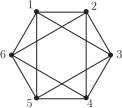
\includegraphics[width=0.33\linewidth]{images/NumberedHexagonalNetwork}
\caption{A possible computer network.\label{HexNet}}
\end{figure}
\end{activity}
\begin{activity}[]\label{activity-318}
In \hyperref[HexNet]{Figure~\ref{HexNet}} we see a graph with six vertices. Suppose we have three different kinds of computers that can be placed at the six vertices of the graph to form a network. In how many different ways may the computers be placed? (Two graphs are not different if we can redraw one of the graphs so that it is identical to the other one.) This is equivalent to permuting the vertices in some way so that when we apply the permutation to the endpoints of the edges to get a new edge set, the new edge set is equal to the old one. Such a permutation is called an \emph{automorphism}\index{automorphism (of a graph)} of the graph. Then two computer placements are the same if there is an automorphism of the graph that carries one to the other.%
\par\medskip\noindent%
\textbf{Solution.}\quad The computer placements are functions from the vertices of the graph to the set of three kinds of computers, say \(\{A,B,C\}\). Thus we are asking for the number of orbits of the automorphism group of the graph on functions from the vertices of \(\{A, B,
C\}\). To find this number we need to compute the cycle index of the automorphism group. An automorphism will send vertices 1, 2, and 3 to three vertices that are mutually connected; i.e. a triangle. Further, each of vertices 4, 5, and 6 is adjacent to exactly two of vertices of 1, 2, and 3. In fact, for any of the eight triangles in the graph, each vertex not in the triangle is adjacent to exactly two vertices of the triangle (and a different two for each vertex). Therefore we can send the vertices 1, 2, and 3, to any of the eight triangles in any of six orders, and this completely determines an automorphism. Thus there are \(6\cdot8=48\) elements in the group of automorphisms. The dihedral group \(D_6\) is a subgroup of the group of automorphisms. The two-cycles \((1\ 4)\), \((2\ 5)\), and \((3\ 6)\) are also in the group of automorphisms. (For example, 1 is adjacent to everything but 4, and 4 is adjacent to everything but 1, so interchanging them leaves us with exactly the same edges.) We will write out \(D_6\) in disjoint cycle notation, and then the coset \((1\ 4)D_6\), and from those we will be able to get the cycle index of the automorphism group acting on the vertices. In cycle notation, \(D_6\) is%
\begin{equation*}
\begin{array}{cccc}
(1\ 2\ 3\ 4\ 5\ 6)\amp (1\ 3\ 5)(2\ 4\ 6)\amp (1\ 4)(2\ 5)(3 \ 6)\amp  (1\ 5\ 3)(2\ 6\ 4)\\(1\ 6\ 5\ 4\
3\ 2)\amp (1)(2)(3)(4)(5)(6)\amp (1)(4)(2\ 6)(3\ 5)\amp (2)(5)(1\ 3)(4\ 6)\\
(3)(6)(1\ 5)(2\ 4)\amp (1\ 2)(3\ 6)(4\ 5)\amp (1\ 6)(2\ 5)(3\ 4)\amp (1\ 4)(2\ 3)(5\ 6)
\end{array}
\end{equation*}
and \((1\ 4)D_6\) is%
\begin{equation*}
\begin{array}{cccc}
(1\ 2\ 3) (4\ 5\ 6)\amp (1\ 3\ 5\ 4\ 6\ 2)\amp (1) (4)(2\ 5)(3 \ 6)\amp  (1\ 5\ 3\ 4\ 2\ 6)\\(1\ 6\
5)(2\ 4\ 3)\amp (1\ 4)(2)(3)(5)(6)\amp (1\ 4)(2\ 6)(3\ 5)\amp (2)(5)(1\ 3\ 4\ 6)\\
(3)(6)(1\ 5\ 4\ 2)\amp (1\ 2\ 4\ 5)(3\ 6)\amp (1\ 6\ 4\ 3)(2\ 5)\amp (1)(4)(2\ 3)(5\ 6).
\end{array}
\end{equation*}
%
\par
Notice that neither \((2\ 5)\) nor \((3\ 6)\) is in the coset, so our group is the union%
\begin{equation*}
D_6\cup (1\ 4)D_6 \cup(2\ 5)D_6 \cup (3\ 6)D_6.
\end{equation*}
%
\par
But by symmetry, the cycle structure of \((1\ 4)D_6\), \((2\ 5)D_6\) and \((3\ 6)D_6\) will be the same, so the cycle index for our group is.%
\begin{equation*}
{1 \over 48} \left(Z^6_1 + 8Z^2_3
+8z_6^1 +7z_2^3+9z_1^2z_2^2 +3z_1^4z_2+
6z_2z_4+6z_1^2z_4\right).
\end{equation*}
%
\par
Since we have three kinds of computers, we substitute 3 for each variable to get%
\begin{equation*}
{1 \over 48} \left(3^6 + 8\cdot3^2
+8\cdot3^1 +7\cdot3^3+9\cdot3^4 +3\cdot3^5+
6\cdot3^2+6\cdot3^3\right)=56.
\end{equation*}
%
\end{activity}
\begin{activity}[]\label{activity-319}
Two simple graphs on the set \([n]= \{1,2,\ldots, n\}\) with edge sets \(E\) and \(E'\) (which we think of a sets of two-element sets for this problem) are said to be \emph{isomorphic} if there is a permutation \(\sigma\) of \([n]\) which, in its action of two-element sets, carries \(E\) to \(E'\). We say two graphs are different if they are not isomorphic. Thus the number of different graphs is the number of orbits of the set of all two-element subsets of \([n]\) under the action of the group \(S_n\). We can represent an edge set by its characteristic function (as in \hyperref[charfunction]{problem~\ref{charfunction}}). That is we define%
\begin{equation*}
\chi_E(\{u,v\}) = \left\{
\begin{array}{ll}
1 \amp  \mbox{if \(\{u,v\}\in E\)} \\
0 \amp  \mbox{otherwise.}
\end{array} \right.
\end{equation*}
%
\par
Thus we can think of the set of graphs as a set of functions defined on the set of all two-element subsets of \([n]\). The number of different graphs with vertex set \([n]\) is thus the number of orbits of this set of characteristic functions under the action of the symmetric group \(S_n\) on the set of two-element subsets of \([n]\). Use this to find the number of different graphs on five vertices.%
\par\medskip\noindent%
\textbf{Solution.}\quad For this problem we need the cycle index for the action of the symmetric group on five letters acting on two-element subsets of those five letters. Each way of partitioning the number five describes the cycle structure of an element of \(S_5\) acting on \([5]\). The cycle structure of a permutation \(\sigma\) on the two-element subsets of \([5]\) will be determined by its cycle structure on \([5]\). The partitions of five and the cycle structures they give on two-element subsets are:%
\leavevmode%
\begin{itemize}[label=\textbullet]
\item{}\((1,1,1,1,1) =1^5\) is the cycle structure of the identity; acting on two-element subsets the identity is a product of \(\binom{5}{2}=10\) one-cycles.  Of course there is only one identity permutation.%
\item{}A permutation with cycle structure \(2^1 1^3\) will fix the two element set in the two cycle and each pair of the three elements outside for a total of four one-cycles; each pair of an element in the two cycle and an element not will be in a two cycle.  There are 6 such pairs and thus three two-cycles, so such a permutation has 3 two-cycles and four one-cycles.  There are \(\binom{5}{2}=10\) such permutations.%
\item{}A permutation with cycle structure \(2^2 1^1\) will have a one-cycle of two-sets for each two cycle, any other two-set will be in a  two cycle.  There are \(4+2+2=8\) such two-sets and thus four two-cycles, so such a permutation has four two cycles and two one cycles.  There are \(\binom{5}{2}\binom{3}{2}/2 =15\) such permutations.%
\item{}A permutation with cycle structure \(3^1 1^2\) will have one cycle of size 1 on two-sets from the two one-element cycles of the original action; each other two-element subset will be in a three cycle.  There are \(\binom{3}{2}+3\cdot2=9\) such pairs, and so there are three three-cycles of two-element subsets.  Thus such a permutation has one one-cycle and three three-cycles in its action of two-sets. There are \(2\binom{5}{3}=20\) such permutations.%
\item{}A permutation with cycle structure \(3^1 2^1\) will have one one-cycle on two-sets from the two-cycle of the original action, it will have \(\binom{3}{2}\)  two-sets in three cycles,  and will have six two-sets in six-cycles, and so will have just one six-cycle of two-sets.  Thus such a permutation has one one-cycle, one three-cycle and one six-cycle when it acts on two-sets.  There are \(2\binom{5}{3}=20\) such permutations.%
\item{}A permutation with cycle structure \(4^1 1^1\) has a four-cycle of two-subsets and one two-cycle of two-subsets from its own four-cycle and another four cycle of pairs of members of the four-cycle and one cycle. thus it has two four-cycles and two one-cycles There are \(6\binom{5}{4}=30\) such permutations.%
\item{}A permutation with cycle structure \(5^1\) will have two five-cycles in its action on two-sets.  There are \(4!=24\) such permutations.%
\end{itemize}
Thus for the group \(S_5\) acting on pairs from \([5]\), the cycle index is%
\begin{equation*}
{1\over120}\left(z_1^{10}+10z_2^3z_1^4+15z_2^4z_2+20z_3^3z_1+20z_6z_3z_1+
30z_4^2z_2+ 24z_5^2\right).
\end{equation*}
%
\par
Substituting 2 for each variable gives us that there are%
\begin{equation*}
{1\over120}\left(2^{10}+10\cdot2^7+15\cdot2^5+20\cdot2^4+20\cdot2^3+30\cdot2^3+
24\cdot2^2\right)=30
\end{equation*}
graphs on five vertices.%
\end{activity}
\typeout{************************************************}
\typeout{Section 5.4 Supplementary Problems}
\typeout{************************************************}
\section[{Supplementary Problems}]{Supplementary Problems}\label{sec_groups-suppprobs}
\leavevmode%
\begin{enumerate}
\item\hypertarget{li-100}{}Show that a function from \(S\) to \(T\) has an inverse (defined on \(T\)) if and only if it is a bijection.%
\item\hypertarget{li-101}{}How many elements are in the dihedral group \(D_3\)?  The symmetric group \(S_3\)?  What can you conclude about \(D_3\) and \(S_3\)?%
\item\hypertarget{li-102}{}A tetrahedron is a thee dimensional geometric figure with four vertices, six edges, and four triangular faces.  Suppose we start with a tetrahedron in space and consider the set of all permutations of the vertices of the tetrahedron that correspond to moving the tetrahedron in space and returning it to its original location, perhaps with the vertices in different places.  Explain why these permutations form a group.  What is the size of this group?  Write down in two-row notation a permutation that is \emph{not} in this group.%
\item\hypertarget{li-103}{}Find a three-element subgroup of the group \(S_3\).  Can you find a different three-element subgroup of \(S_3\)?%
\item\hypertarget{li-104}{}Prove true or demonstrate false with a counterexample:  ``In a permutation group, \((\sigma\varphi)^n = \sigma^n\varphi^n\).''%
\item\hypertarget{li-105}{}Describe a permutation group with 60 elements.%
\item\hypertarget{li-106}{}If a group \(G\) acts on a set \(S\), and if \(\sigma(x) =y\), is there anything interesting we can say about the subgroups \({ Fix}(x)\) and \({ Fix}(y)\)?%
\item\hypertarget{li-107}{}Find the number of ways to color the faces of a tetrahedron with two colors.%
\item\hypertarget{li-108}{}Find the number of ways to color the faces of a tetrahedron with four colors so that each color is used.%
\item\hypertarget{li-109}{}Find the cycle index of the group of spatial symmetries of the tetrahedron acting on the vertices.  Find the cycle index for the same group acting on the faces.%
\item\hypertarget{li-110}{}Find the generating function for the number of ways to color the faces of the tetrahedron with red, blue, green and yellow.%
\item\hypertarget{li-111}{}(interesting) Find the generating function for the number of ways to color the faces of a cube with four colors so that all four colors are used.%
\item\hypertarget{li-112}{}(interesting) How many different graphs are there on six vertices with seven edges?%
\end{enumerate}
\appendix%
%
%% A lineskip in table of contents as transition to appendices, backmatter
\addtocontents{toc}{\vspace{\normalbaselineskip}}
%
%
\appendix
%
\typeout{************************************************}
\typeout{Appendix A Relations}
\typeout{************************************************}
\chapter[{Relations}]{Relations}\label{Relations}
\typeout{************************************************}
\typeout{Section  Relations as sets of Ordered Pairs}
\typeout{************************************************}
\section[{Relations as sets of Ordered Pairs}]{Relations as sets of Ordered Pairs}\label{section-22}
\typeout{************************************************}
\typeout{Subsection  The relation of a function}
\typeout{************************************************}
\subsection[{The relation of a function}]{The relation of a function}\label{functionrelation}
\begin{activity}[]\label{functionsasorderedpairs}
Consider the functions from \(S=\{-2,-1,0,1,2\}\) to \(T=\{1,2,3,4,5\}\) defined by \(f(x) = x+3\), and \(g(x) = x^5-5x^3+5x +3\). Write down the set of ordered pairs \((x,f(x))\) for \(x \in S\) and the set of ordered pairs \((x,g(x))\) for \(x \in S\). Are the two functions the same or different?%
\par\medskip\noindent%
\textbf{Solution.}\quad We get \(\{(-2,1),(-1,2),(0,3),(1,4),(2,5)\}\) in both cases, so the functions are the same.%
\end{activity}
\hyperref[functionsasorderedpairs]{Problem~\ref{functionsasorderedpairs}} points out how two functions which appear to be different are actually the same on some domain of interest to us. Most of the time when we are thinking about functions it is fine to think of a function casually as a relationship between two sets. In \hyperref[functionsasorderedpairs]{Problem~\ref{functionsasorderedpairs}} the set of ordered pairs you wrote down for each function is called the \index{relation!of a function}\index{function!relation of}\emph{relation} of the function. When we want to distinguish between the casual and the careful in talking about relationships, our casual term will be ``relationship'' and our careful term will be ``relation.'' So \emph{relation} is a technical word in mathematics, and as such it has a technical definition. A \index{relation}\emph{relation} from a set \(S\) to a set \(T\) is a set of ordered pairs whose first elements are in \(S\) and whose second elements are in \(T\). Another way to say this is that a \emph{relation} from \(S\) to \(T\) is a subset of \(S\times T\).%
\par
A typical way to define a \emph{function}\index{function} \(f\) from a set \(S\) to a set \(T\) is that \(f\) is a relationship between \(S\) to \(T\) that relates one and only one member of \(T\) to each element of \(X\). We use \(f(x)\) to stand for the element of \(T\) that is related to the element \(x\) of \(S\). If we wanted to make our definition more precise, we could substitute the word ``relation'' for the word ``relationship'' and we would have a more precise definition. For our purposes, you can choose whichever definition you prefer. However, in any case, there is a relation associated with each function. As we said above, the relation of a function \(f:
S\rightarrow T\) (which is the standard shorthand for ``\(f\) is a function from \(S\) to \(T\)'' and is usually read as \(f\) \emph{maps} \(S\) to \(T\)) is the set of all ordered pairs \((x,f(x))\) such that \(x\) is in \(S\).%
\begin{activity}[]\label{formalrelations}
~\par
\begin{enumerate}[label=(\alph*)]
 \item Here are some questions that will help you get used to the formal idea of a relation and the related formal idea of a function. \(S\) will stand for a set of size \(s\) and \(T\) will stand for a set of size \(t\).%
~\par
\begin{enumerate}[label=(\alph*)]
 \item What is the size of the largest relation from \(S\) to \(T\)?%
\par\medskip\noindent%
\textbf{Solution.}\quad \(st\) because that is the size of the relation that has all the ordered pairs \((x,y)\) with \(x\in S\) and \(y\in T\).%

~\par
\item What is the size of the smallest relation from \(S\) to \(T\)?%
\par\medskip\noindent%
\textbf{Solution.}\quad 0, because the empty set of ordered pairs is a relation.%

~\par
\item The relation of a function \(f:S\rightarrow T\) is the set of all ordered pairs \((x,f(x))\) with \(x\in S\).  What is the size of the relation of a function from \(S\) to \(T\)?  That is, how many ordered pairs are in the relation of a function from \(S\) to \(T\)?%
\par\medskip\noindent%
\textbf{Solution.}\quad The size of the relation of \(f:S\rightarrow T\) is \(s\).%

~\par
\item We say \(f\) is a \emph{one-to-one}\index{function!one-to-one}\index{one-to-one function}\index{injection} function or \emph{injection} from \(S\) to \(T\) if each member of \(S\) is related to a \emph{different} element of \(T\). How many different elements must appear as second elements of the ordered pairs in the relation of a one-to-one function (injection) from \(S\) to \(T\)?%
\par\medskip\noindent%
\textbf{Solution.}\quad \(s\) different elements must appear, one for each element of \(S\).%

~\par
\item A function \(f:S\rightarrow T\) is called an \index{onto function}\index{function!onto}\emph{onto function} or \index{surjection}\index{function!surjection}\emph{surjection} if each element of \(T\) is \(f(x)\) for some \(x\in S\) What is the minimum size that \(S\) can have if there is a  surjection from \(S\) to \(T\)?%
\par\medskip\noindent%
\textbf{Solution.}\quad In order to have a surjection from \(S\) to \(T\), the size of \(S\) must be at least \(t\).%

\end{enumerate}
\item When \(f\) is a function from \(S\) to \(T\), the sets \(S\) and \(T\) play a big role in determining whether a function is one-to-one or onto (as defined in \hyperref[formalrelations]{Problem~\ref{formalrelations}}). For example, if \(S\) and \(T\) are both the nonnegative real numbers, and \(f:S\rightarrow T\) is given by \(f(x) =x^2\), is \(f\) one-to-one? Is \(f\) onto? Now assume \(S'\) is the set of all real numbers and \(g:S'\rightarrow T\) is given by \(g(x) = x^2\). Is \(g\) one-to-one? Is \(g\) onto? Assume that \(T'\) is the set of all real numbers and \(h:S\rightarrow T'\) is given by \(h(x) = x^2\). Is \(h\) one-to-one? Is \(h\) onto? And if the function \(j:S'\rightarrow T'\) is given by \(j(x)=x^2\), is \(j\) one-to-one? Is \(j\) onto?%
\par\medskip\noindent%
\textbf{Solution.}\quad With \(S\) as domain, \(f\) is both one-to-one and onto. The function \(g\) is not one-to-one, but it is onto. The function \(h\) is one-to-one but not onto. The function \(j\) is neither one-to-one nor onto.%

~\par
\item If \(f:S\rightarrow T\) is a function, we say that \(f\)\emph{maps} \(x\) to \(y\) as another way to say that \(f(x)=y\). Suppose \(S=T=\{1,2,3\}\). Give a function from \(S\) to \(T\) that is not onto. Notice that two different members of \(S\) have mapped to the same element of \(T\). Thus when we say that \(f\) associates one and only one element of \(T\) to each element of \(S\), it is quite possible that the one and only one element \(f(1)\) that \(f\) maps 1 to is exactly the same as the one and only one element \(f(2)\) that \(f\) maps 2 to.%
\par\medskip\noindent%
\textbf{Solution.}\quad The function given by \(f(x)=1\) for all \(x\) in \(S\) is not onto.%

\end{enumerate}
\end{activity}
\typeout{************************************************}
\typeout{Subsection  Directed graphs}
\typeout{************************************************}
\subsection[{Directed graphs}]{Directed graphs}\label{relationdigraph}
We visualize numerical functions like \(f(x)=x^2\) with their graphs in Cartesian coordinate systems. We will call these kinds of graphs \index{graph!coordinate}\emph{coordinate graphs} to distinguish them from other kinds of graphs used to visualize relations that are non-numerical.%
\begin{figure}
\centering
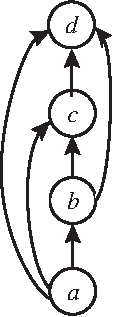
\includegraphics[width=0.1\linewidth]{images/alphabetdigraph}
\caption{The alphabet digraph.\label{alphabetdigraph}}
\end{figure}
In \hyperref[alphabetdigraph]{Figure~\ref{alphabetdigraph}} we illustrate another kind of graph, a ``directed graph'' or ``digraph'' of the ``comes before in alphabetical order" relation on the letters \(a\), \(b\), \(c\), and \(d\). To draw a \index{graph!directed}\index{directed graph}\index{digraph}\emph{directed graph} of a relation on a set \(S\), we draw a circle (or dot, if we prefer), which we call a \index{vertex}\emph{vertex}\index{vertex!of a complete graph}, for each element of the set, we usually label the vertex with the set element it corresponds to, and we draw an arrow from the vertex for \(a\) to that for \(b\) if \(a\) is related to \(b\), that is, if the ordered pair \((a,b)\) is in our relation. We call such an arrow an \index{edge}\emph{edge}\index{edge!in a digraph} or a \emph{directed edge}. We draw the arrow from \(a\) to \(b\), for example, because \(a\) comes before \(b\) in alphabetical order. We try to choose the locations where we draw our vertices so that the arrows capture what we are trying to illustrate as well as possible. Sometimes this entails redrawing our directed graph several times until we think the arrows capture the relationship well.%
\par
We also draw digraphs for relations from a set \(S\) to a set \(T\); we simply draw vertices for the elements of \(S\) (usually in a row) and vertices for the elements of \(T\) (usually in a parallel row) draw an arrow from \(x\) in \(S\) to \(y\) in \(T\) if \(x\) is related to \(y\). Notice that instead of referring to the vertex representing \(x\), we simply referred to \(x\). This is a common shorthand. Here are some exercises just to practice drawing digraphs.%
\begin{activity}[]\label{activity-322}
~\par
\begin{enumerate}[label=(\alph*)]
 \item Draw the digraph of the ``is a proper subset of'' relation on the set of subsets of a two element set. How many arrows would you have had to draw if this problem asked you to draw the digraph for the subsets of a three-element set?%
\par\medskip\noindent%
\textbf{Solution.}\quad \mbox{ 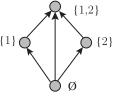
\includegraphics[width=0.2\linewidth]{images/Subsetsof2set}
 } We would need to draw 19 arrows, some of them curved, for the subsets of a three-element set.%

~\par
\item Draw the digraph of the relation from the set \{A, M, P, S\} to the set \{Sam, Mary, Pat, Ann, Polly, Sarah\} given by ``is the first letter of.''%
\par\medskip\noindent%
\textbf{Solution.}\quad 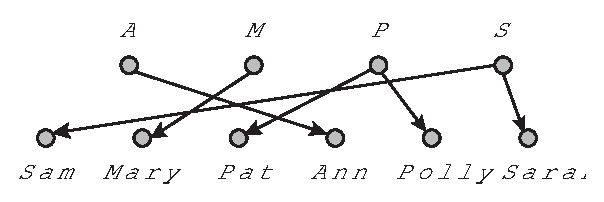
\includegraphics[width=0.5\linewidth]{images/initialdigraph}
%

\end{enumerate}
\end{activity}
\typeout{************************************************}
\typeout{Subsection  Digraphs of Functions}
\typeout{************************************************}
\subsection[{Digraphs of Functions}]{Digraphs of Functions}\label{digraphsoffunctions}
\emph{Need to crosscheck some references back in 1.2.2, since they likely aren't to the right thing at this point.}%
\typeout{************************************************}
\typeout{Subsection  Equivalence relations}
\typeout{************************************************}
\subsection[{Equivalence relations}]{Equivalence relations}\label{equivalencerelations}
So far we've used relations primarily to talk about functions. There is another kind of relation, called an equivalence relation, that comes up in the counting problems with which we began. In \hyperref[icecreaminpints]{Problem~\ref{icecreaminpints}} with three distinct flavors, it was probably tempting to say there are 12 flavors for the first pint, 11 for the second, and 10 for the third, so there are \(12\cdot 11\cdot 10\) ways to choose the pints of ice cream. However, once the pints have been chosen, bought, and put into a bag, there is no way to tell which is first, which is second and which is third. What we just counted is lists of three distinct flavors\textemdash{}one to one functions from the set \(\{1,2,3\}\) in to the set of ice cream flavors. Two of those lists become equivalent once the ice cream purchase is made if they list the same ice cream. In other words, two of those lists become equivalent (are related) if they list same subset of the set of ice cream flavors. To visualize this relation with a digraph, we would need one vertex for each of the \(12\cdot 11\cdot 10\) lists. Even with five flavors of ice cream, we would need one vertex for each of \(5\cdot4\cdot3=60\) lists. So for now we will work with the easier to draw question of choosing three pints of ice cream of different flavors from four flavors of ice cream.%
\begin{activity}[]\label{fourchoosethree}
Suppose we have four flavors of ice cream, V(anilla), C(hocolate), S(trawberry) and P(each). Draw the directed graph whose vertices consist of all lists of three distinct flavors of the ice cream, and whose edges connect two lists if they list the same three flavors. This graph makes it pretty clear in how many ways we may choose 3 flavors out of four. How many is it?%
\par\medskip\noindent%
\textbf{Solution.}\quad We used double-headed arrows in place of one arrow going in each direction to reduce the clutter in the picture. Note that there is an arrow from each vertex to itself. We may choose 3 flavors in four ways.%
\par
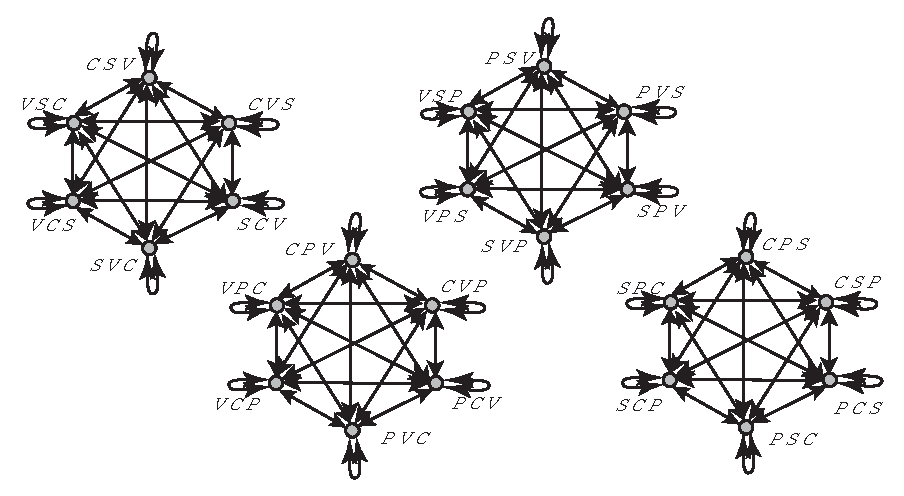
\includegraphics[width=0.7\linewidth]{images/flavordigraph}
%
\end{activity}
\begin{activity}[]\label{icecreaminadish}
Now suppose again we are choosing three distinct flavors of ice cream out of four, but instead of putting scoops in a cone or choosing pints, we are going to have the three scoops arranged symmetrically in a circular dish. Similarly to choosing three pints, we can describe a selection of ice cream in terms of which one goes in the dish first, which one goes in second (say to the right of the first), and which one goes in third (say to the right of the second scoop, which makes it to the left of the first scoop). But again, two of these lists will sometimes be equivalent. Once they are in the dish, we can't tell which one went in first. However, there is a subtle difference between putting each flavor in its own small dish and putting all three flavors in a circle in a larger dish. Think about what makes the lists of flavors equivalent, and draw the directed graph whose vertices consist of all lists of three of the flavors of ice cream and whose edges connect two lists that we cannot tell the difference between as dishes of ice cream. How many dishes of ice cream can we distinguish from one another?%
\par\medskip\noindent%
\textbf{Solution.}\quad We can distinguish eight different dishes of ice cream.%
\par
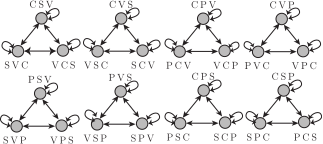
\includegraphics[width=0.7\linewidth]{images/icecreamindish}
%
\end{activity}
\begin{activity}[]\label{activity-325}
Draw the digraph for \hyperref[roundtable]{Problem~\ref{roundtable}} in the special case where we have four people sitting around the table.%
\par\medskip\noindent%
\textbf{Solution.}\quad 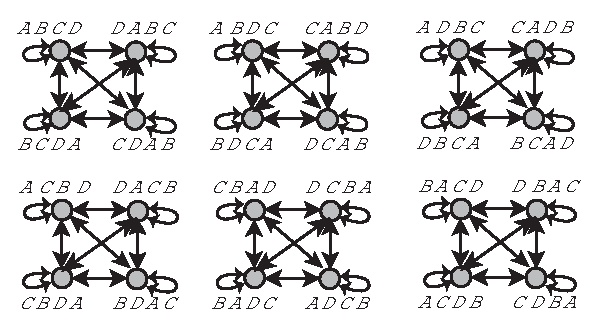
\includegraphics[width=0.7\linewidth]{images/4AROUNDATABLE}
\end{activity}
In \hyperref[fourchoosethree]{Problems~\ref{fourchoosethree}}, \hyperref[icecreaminadish]{Activity~\ref{icecreaminadish}}, and {$\langle\langle$Unresolved xref, reference "roundtablefour"; check spelling or use "provisional" attribute$\rangle\rangle$} (as well as \hyperref[twelvechoosethree]{Problems~\ref{twelvechoosethree}}, \hyperref[roundtable]{Activity~\ref{roundtable}}, and \hyperref[formulanchoosek]{Activity~\ref{formulanchoosek}}) we can begin with a set of lists, and say when two lists are equivalent as representations of the objects we are trying to count. In particular, in \hyperref[fourchoosethree]{Problems~\ref{fourchoosethree}}, \hyperref[icecreaminadish]{Activity~\ref{icecreaminadish}}, and {$\langle\langle$Unresolved xref, reference "roundtablefour"; check spelling or use "provisional" attribute$\rangle\rangle$} you drew the directed graph for this relation of equivalence. Technically, you should have had an arrow from each vertex (list) to itself. This is what we mean when we say a relation is \emph{reflexive}. Whenever you had an arrow from one vertex to a second, you had an arrow back to the first. This is what we mean when we say a relation is \emph{symmetric}.%
\par
When people sit around a round table, each list is equivalent to itself: if List1 and List 2 are identical, then everyone has the same person to the right in both lists (including the first person in the list being to the right of the last person). To see the symmetric property of the equivalence of seating arrangements, if List1 and List2 are different, but everyone has the same person to the right when they sit according to List2 as when they sit according to List1, then everybody better have the same person to the right when they sit according to List1 as when they sit according to List2.%
\par
In \hyperref[fourchoosethree]{Problems~\ref{fourchoosethree}}, \hyperref[icecreaminadish]{Activity~\ref{icecreaminadish}} and {$\langle\langle$Unresolved xref, reference "roundtablefour"; check spelling or use "provisional" attribute$\rangle\rangle$} there is another property of those relations you may have noticed from the directed graph. Whenever you had an arrow from \(L_1\) to \(L_2\) and an arrow from \(L_2\) to \(L_3\), then there was an arrow from \(L_1\) to \(L_3\). This is what we mean when we say a relation is \emph{transitive}. You also undoubtedly noticed how the directed graph divides up into clumps of mutually connected vertices. This is what equivalence relations are all about. Let's be a bit more precise in our description of what it means for a relation to be reflexive, symmetric or transitive. \leavevmode%
\begin{itemize}[label=\textbullet]
\item{}If \(R\) is a relation on a set \(X\), we say \(R\) is \index{reflexive}\index{relation!reflexive}\emph{reflexive}  if \((x,x)\in
R\) for every \(x\in X\).%
\item{}If \(R\) is a relation on a set \(X\), we say \(R\) is \index{symmetric}\index{relation!reflexive}\emph{symmetric} if \((x,y)\) is in \(R\) whenever \((y,x)\) is in \(R\).%
\item{}If \(R\) is a relation on a set \(X\), we say \(R\) is \index{transitive}\index{relation!transitive}\emph{transitive} if whenever \((x,y)\) is in \(R\) and \((y,z)\) is in \(R\), then \((x,z)\) is in \(R\) as well.%
\end{itemize}
%
\par
Each of the relations of equivalence you worked with in the \hyperref[fourchoosethree]{Problem~\ref{fourchoosethree}}, \hyperref[icecreaminadish]{Activity~\ref{icecreaminadish}} and {$\langle\langle$Unresolved xref, reference "roundtablefour"; check spelling or use "provisional" attribute$\rangle\rangle$} had these three properties. Can you visualize the same three properties in the relations of equivalence that you would use in \hyperref[twelvechoosethree]{problems~\ref{twelvechoosethree}}, \hyperref[roundtable]{Activity~\ref{roundtable}}, and \hyperref[formulanchoosek]{Activity~\ref{formulanchoosek}}? We call a relation an \emph{equivalence relation}\index{equivalence relation}\index{relation!equivalence} if it is reflexive, symmetric and transitive.%
\par
After some more examples, we will see how to show that equivalence relations have the kind of clumping property you saw in the directed graphs. In our first example, using the notation \((a,b) \in R\) to say that \(a\) is related to \(B\) is going to get in the way. It is really more common to write \(a
R b\) to mean that \(a\) is related to \(b\). For example, if our relation is the less than relation on \(\{1,2,3\}\), you are much more likely to use \(x\lt y\) than you are \((x,y)\in \ \lt\), aren't you? The reflexive law then says \(xRx\) for every \(x\) in \(X\), the symmetric law says that if \(xRy\), then \(yRx\), and the transitive law says that if \(xRy\) and \(yRz\), then \(xRz\).%
\begin{activity}[]\label{nchoosekanotherway}
~\par
\begin{enumerate}[label=(\alph*)]
 \item For the necklace problem, \hyperref[necklace]{Problem~\ref{necklace}}, our lists are lists of beads. What makes two lists equivalent for the purpose of describing a necklace? Verify explicitly that this relationship of equivalence is reflexive, symmetric, and transitive.%
\par\medskip\noindent%
\textbf{Solution.}\quad Two lists are equivalent if I can get one from the other by some combination of cyclic permutations (putting the last thing in the list at the front and moving everything else one place right) and reversals. The combination could include no operation at all. Since it is possible to have no operation, the relation is reflexive. (Even without the opportunity to do no operation, if we do two reversals to a list we get the original list back so it is equivalent to itself.) Suppose we have \(n\) beads. Then if I can get from list \(A\) to list \(B\) with a cyclic permutations, then \(n-1\) more cyclic permutations give us the original list. Also if I get from a list \(A\) to a list \(B\) by a reversal, then another reversal takes \(B\) to \(A\). Thus any sequence of cyclic permutations and reversals can be undone. Therefore if list \(A\) is equivalent to list \(B\), then list \(B\) is equivalent to list \(A\). Following one combination of operations with another one still gives a combination of operations, so our relation is transitive.%

~\par
\item Which of the reflexive, symmetric and transitive properties does the \(\lt\) relation on the integers have?%
\par\medskip\noindent%
\textbf{Solution.}\quad It is transitive, but not reflexive or symmetric.%

~\par
\item A relation \(R\) on the set of ordered pairs of positive integers that you learned about in grade school in another notation is the relation that says \((m,n)\) is related to \((h,k)\) if \(mk =hn\). Show that this relation is an equivalence relation. In what context did you learn about this relation in grade school?%
\par\medskip\noindent%
\textbf{Solution.}\quad \(mn=mn\) so the relation is reflexive. If \(mk=hn\), then \(hn=mk\), so if \((m,n)\) is related to \((h,k)\), then \((h,k)\) is related to \((m,n)\). If \((m,n)\) is related to \((h,k)\) and \((h,k)\) is related to \((p,q)\), then \(mk=hn\) and \(hq=pk\), which gives us \(mkhq=hnpk\), and cancelling \(h\) and \(k\) gives us \(mq=np=pn\), so \((m,n)\) is related to \((p,q)\). Therefore, the relation is transitive. This is the relation of equality of the fractions \(m\over n\) and \(h\over k\).%

~\par
\item Another relation that you may have learned about in school, perhaps in the guise of ``clock arithmetic,'' is the relation of equivalence modulo \(n\). For integers (positive, negative, or zero) \(a\) and \(b\), we write \(a
\equiv b \pmod{n}\) to mean that \(a-b\) is an integer multiple of \(n\), and in this case, we say that \(a\) is \index{congruence modulo \(n\)}\emph{congruent to \(b\) modulo \(n\)} and write \(a\equiv b \pmod{n}\).. Show that the relation of congruence modulo \(n\) is an equivalence relation.%
\par\medskip\noindent%
\textbf{Solution.}\quad \(a-a=0=0\cdot n\), so \(a\equiv a\pmod{n}\). Thus the relation is reflexive. If \(a-b=kn\) for some integer \(k\), then \(b-a=-kn\), and -k is an integer, so if \(a\equiv b \pmod{n}\), then \(b\equiv a \pmod{n}\). If \(a-b=kn\) and \(b-c= jn\), then \(a-b+b-c=kn+jn\), so \(a-c=(k+j)n\) and since \(k+j\) is an integer this means that \(a\equiv c\pmod{n}\). Therefore the relation of congruence mod \(n\) is an equivalence relation.%

~\par
\item Define a relation on the set of all lists of \(n\) distinct integers chosen from \(\{1,2,\ldots, n\}\), by saying two lists are related if they have the same elements (though perhaps in a different order) in the first \(k\) places, and the same elements (though perhaps in a different order) in the last \(n-k\) places. Show this relation is an equivalence relation.%
\par\medskip\noindent%
\textbf{Solution.}\quad The relation is reflexive, for a list \(L\) has the same elements as the list \(L\) in the first \(k\) places and the last \(n-k\) places. If \(L_1\) and \(L_2\) have the same elements in the first \(k\) places and have the same elements in the last \(k\) places, then \(L_2\) and \(L_1\) have the same elements in the first \(k\) places and have the same elements in the last \(n-k\) places, so our relation is symmetric. If \(L_1\) and \(L_2\) have the same elements in the first \(k\) places and \(L_2\) and \(L_3\) have the same elements in the first \(k\) places, then \(L_1\) and \(L_3\) have the same elements in the first \(k\) places. Similarly with the last \(n-k\) places. Therefore our relation is transitive, and so it is an equivalence relation.%

~\par
\item Suppose that \(R\) is an equivalence relation on a set \(X\) and for each \(x\in X\), let \(C_x = \{y| y\in X \mbox{ and } 
yRx\}\). If \(C_x\) and \(C_z\) have an element \(y\) in common, what can you conclude about \(C_x\) and \(C_z\) (besides the fact that they have an element in common!)? Be explicit about what property(ies) of equivalence relations justify your answer. Why is every element of \(X\) in some set \(C_x\)? Be explicit about what property(ies) of equivalence relations you are using to answer this question. Notice that we might simultaneously denote a set by \(C_x\) and \(C_y\). Explain why the union of the sets \(C_x\) is \(X\). Explain why two distinct sets \(C_x\) and \(C_z\) are disjoint. What do these sets have to do with the ``clumping'' you saw in the digraph of \hyperref[fourchoosethree]{Problem~\ref{fourchoosethree}} and \hyperref[icecreaminadish]{Activity~\ref{icecreaminadish}}?%
\par\medskip\noindent%
\textbf{Solution.}\quad If \(C_x\) and \(C_y\) have the element \(z\) in common, then by symmetry and transitivity, all elements in \(C_x\) are related to \(z\) and by symmetry and transitivity, all elements in \(C_y\) are related to \(z\). Then by symmetry and transitivity again, all elements of \(C_y\) are related to \(x\), so \(C_y\subseteq C_x\). By the same kind of reasoning, \(C_x\subseteq C_y\). Therefore, \(C_x=C_y\). Every element \(x\) is in the set \(C_x\) by reflexivity Thus the union of the sets \(C_x\) is \(X\). The sets \(C_x\) and \(C_y\) are disjoint if they are different, because if they have a common element \(z\) then they are equal. By definition, the sets \(C_x\) form a partition of \(X\). The clumps that we saw in those problems are the blocks of the partition.%

\end{enumerate}
\end{activity}
In {$\langle\langle$Unresolved xref, reference "equivalenceclasses"; check spelling or use "provisional" attribute$\rangle\rangle$} the sets \(C_x\) are called \index{equivalence class}\emph{equivalence classes} of the equivalence relation \(R\). You have just proved that if \(R\) is an equivalence relation of the set \(X\), then each element of \(X\) is in exactly one equivalence class of \(R\). Recall that a \index{partition (of a set)}\emph{partition} of a set \(X\) is a set of disjoint sets whose union is \(X\). For example, \(\{1,3\}\), \(\{2,4,6\}\), \(\{5\}\) is a partition of the set \(\{1,2,3,4,5,6\}\). Thus another way to describe what you proved in {$\langle\langle$Unresolved xref, reference "equivalenceclasses"; check spelling or use "provisional" attribute$\rangle\rangle$} is the following:%
\begin{theorem}[{}]\label{theorem-9}
If \(R\) is an equivalence relation on \(X\), then the set of equivalence classes of \(R\) is a partition of \(X\).%
\end{theorem}
Since a partition of \(S\) is a set of subsets of \(S\), it is common to call the subsets into which we partition \(S\) the \index{block of a partition}\emph{blocks} of the partition so that we don't find ourselves in the uncomfortable position of referring to a set and not being sure whether it is the set being partitioned or one of the blocks of the partition.%
\begin{activity}[]\label{partitiontoequivalence}
~\par
\begin{enumerate}[label=(\alph*)]
 \item In each of \hyperref[roundtable]{Problems~\ref{roundtable}}, \hyperref[formulanchoosek]{Activity~\ref{formulanchoosek}}, \hyperref[necklace]{Activity~\ref{necklace}}, \hyperref[fourchoosethree]{Activity~\ref{fourchoosethree}}, and \hyperref[icecreaminadish]{Activity~\ref{icecreaminadish}}, what does an equivalence class correspond to? (Five answers are expected here.)%
\par\medskip\noindent%
\textbf{Solution.}\quad In \hyperref[roundtable]{Problem~\ref{roundtable}} the equivalence classes correspond to seating arrangements. In \hyperref[formulanchoosek]{Problem~\ref{formulanchoosek}} the equivalence classes correspond to the \(k\)-element subsets of our \(n\)-element set \(S\). In \hyperref[necklace]{Problem~\ref{necklace}}, the equivalence classes correspond to necklaces. In \hyperref[fourchoosethree]{Problem~\ref{fourchoosethree}} the equivalence classes correspond to choices of three flavors of ice cream out of a possible four flavors. In \hyperref[icecreaminadish]{Problem~\ref{icecreaminadish}} the equivalence classes correspond to the ways we can choose scoops of ice cream of three different flavors out of four and put them into a dish in a symmetric fashion.%

~\par
\item Given the partition \(\{1,3\}\), \(\{2,4,6\}\), \(\{5\}\) of the set \(\{1,2,3,4,5,6\}\), define two elements of \(\{1,2,3,4,5,6\}\) to be related if they are in the same part of the partition. That is, define 1 to be related to 3 (and 1 and 3 each related to itself), define 2 and 4, 2 and 6, and 4 and 6 to be related (and each of 2, 4, and 6 to be related to itself), and define 5 to be related to itself. Show that this relation is an equivalence relation.%
\par\medskip\noindent%
\textbf{Solution.}\quad We have said for each element of our set that it is related to itself, so the relation is reflexive. If \(x\) and \(y\) are in a given one of those sets, then \(y\) and \(x\) are in that same given set. If \(x\) and \(y\) are in the same set, and if \(y\) and \(z\) are in the same set, then \(x\) and \(z\) must be in the same set because there is one and only one set that \(y\) is in. Thus the relation is an equivalence relation.%

~\par
\item Suppose \(P = \{S_1, S_2, S_3, \ldots, S_k\}\) is a partition of \(S\). Define two elements of \(S\) to be related if they are in the same set \(S_i\), and otherwise not to be related. Show that this relation is an equivalence relation. Show that the equivalence classes of the equivalence relation are the sets \(S_i\).%
\par\medskip\noindent%
\textbf{Solution.}\quad Each element is in a set \(S_i\) with itself, so the relation is reflexive. If \(x\) and \(y\) are in a given one of those sets \(S_i\), then \(y\) and \(x\) are in that same set \(S_i\). If \(x\) and \(y\) are in the same set \(S_i\), and if \(y\) and \(z\) are in the same set \(S_j\), then \(S_i\) must equal \(S_j\) because \(y\) is in one and only one block of the partition. Therefore, \(x\) and \(z\) must be in the same set \(S_i\). Thus the relation is an equivalence relation. If \(x\in S_i\), then by definition \(S_i\) consists of all elements related to \(x\), so it is the equivalence class containing \(x\).%

\end{enumerate}
\end{activity}
In \hyperref[partitiontoequivalence]{Problem~\ref{partitiontoequivalence}} you just proved that each partition of a set gives rise to an equivalence relation whose classes are just the parts of the partition. Thus in {$\langle\langle$Unresolved xref, reference "equivalenceclasses"; check spelling or use "provisional" attribute$\rangle\rangle$} and \hyperref[partitiontoequivalence]{Problem~\ref{partitiontoequivalence}} you proved the following Theorem.%
\begin{theorem}[{}]\label{theorem-10}
A relation \(R\) is an equivalence relation on a set \(S\) if and only if \(S\) may be partitioned into sets \(S_1\), \(S_2\), \dots{}, \(S_n\) in such a way that \(x\) and \(y\) are related by \(R\) if and only if they are in the same block \(S_i\) of the partition.%
\end{theorem}
\index{equivalence relation}\index{relation!equivalence}%
\par
In \hyperref[fourchoosethree]{Problems~\ref{fourchoosethree}}, \hyperref[icecreaminadish]{Activity~\ref{icecreaminadish}}, \hyperref[roundtable]{Activity~\ref{roundtable}} and \hyperref[necklace]{Activity~\ref{necklace}} what we were doing in each case was counting equivalence classes of an equivalence relation. There was a special structure to the problems that made this somewhat easier to do. For example, in \hyperref[fourchoosethree]{Activity~\ref{fourchoosethree}}, we had \(4\cdot3\cdot2 =24\) lists of three distinct flavors chosen from V, C, S, and P. Each list was equivalent to \(3\cdot2\cdot1=3!=6\) lists, including itself, from the point of view of serving 3 small dishes of ice cream. The order in which we selected the three flavors was unimportant. Thus the set of all \(4\cdot3\cdot2\) lists was a union of some number \(n\) of equivalence classes, each of size 6. By the product principle, if we have a union of \(n\) disjoint sets, each of size 6, the union has \(6n\) elements. But we already knew that the union was the set of all 24 lists of three distinct letters chosen from our four letters. Thus we have \(6n=24\), or \(n=4\) equivalence classes.%
\par
In \hyperref[icecreaminadish]{Problem~\ref{icecreaminadish}} there is a subtle change. In the language we adopted for seating people around a round table, if we choose the flavors V, C, and S, and arrange them in the dish with C to the right of V and S to the right of C, then the scoops are in different relative positions than if we arrange them instead with S to the right of V and C to the right of S. Thus the order in which the scoops go into the dish is somewhat important\textemdash{}somewhat, because putting in V first, then C to its right and S to its right is the same as putting in S first, then V to its right and C to its right. In this case, each list of three flavors is equivalent to only three lists, including itself, and so if there are \(n\) equivalence classes, we have \(3n=24\), so there are \(24/3=8\) equivalence classes.%
\begin{activity}[]\label{EquivPrincipleProblem}
~\par
\begin{enumerate}[label=(\alph*)]
 \item If we have an equivalence relation that divides a set with \(k\) elements up into equivalence classes each of size \(m\), what is the number \(n\) of equivalence classes? Explain why.%
\par\medskip\noindent%
\textbf{Solution.}\quad The number of equivalence classes is \(k/m\), because by the product principle, \(mn=k\).%

~\par
\item In \hyperref[nchoosekanotherway]{Problem~\ref{nchoosekanotherway}}, what is the number of equivalence classes? Explain in words the relationship between this problem and the \hyperref[formulanchoosek]{Problem~\ref{formulanchoosek}}.%
\par\medskip\noindent%
\textbf{Solution.}\quad There are \(n!\) lists, and each is in an equivalence class of size \(k!(n-k)!\), so the number of equivalence classes is \(n!\over k!(n-k)!\) by \hyperref[EquivPrincipleProblem]{Problem~\ref{EquivPrincipleProblem}}. This is a way of computing the number of \(k\)-element subsets that shows why the final answer we got in \hyperref[formulanchoosek]{Problem~\ref{formulanchoosek}} is symmetric in \(k\) and \(n-k\).%

~\par
\item Describe explicitly what makes two lists of beads equivalent in \hyperref[necklace]{Problem~\ref{necklace}} and how \hyperref[EquivPrincipleProblem]{Problem~\ref{EquivPrincipleProblem}} can be used to compute the number of different necklaces.%
\par\medskip\noindent%
\textbf{Solution.}\quad Two lists are equivalent if I can get one from the other by some combination of cyclic shifts and reversals. A cyclic shift on the list \(a_1,a_2,\ldots,a_{n-1},a_n\) gives either the list \(a_n,a_1,a_2,\ldots ,a_{n-1}\) or the list \(a_2,\ldots,a_{n-1},a_n,a_1\). There are \(n\) possible results of repeated cyclic shifts, and each of them may be reversed to give a new list if \(n\ge 3\). Further, these are the only lists we can get from shifts and reversals. (\(a_1\) must go to one of \(n\) places, and that leaves two choices for where \(a_2\) goes. Then the rest of the list is determined.) Thus we can get exactly \(2n\) lists from combinations of cyclic shifts and reversals. We define two lists to be equivalent if they give the same necklace; we've seen that this is an equivalence relation and that it has \(2n\) elements per equivalence class. Since there are \(n!\) lists, this gives us \((n-1)!/2\) equivalence classes, or necklaces.%

~\par
\item What are the equivalence classes (write them out as sets of lists) in \hyperref[twocolorsofbeads]{Problem~\ref{twocolorsofbeads}}, and why can't we use \hyperref[EquivPrincipleProblem]{Problem~\ref{EquivPrincipleProblem}} to compute the number of equivalence classes?%
\par\medskip\noindent%
\textbf{Solution.}\quad The equivalence classes are%
\begin{equation*}
\{RRBB, BRRB, BBRR, RBBR\}
\mbox{~and~} 
\{RBRB, BRBR\}.
\end{equation*}
%
\par
We can't use \hyperref[EquivPrincipleProblem]{Problem~\ref{EquivPrincipleProblem}} to compute the number of equivalence classes because the equivalence classes don't have the same size.%

\end{enumerate}
\end{activity}
In \hyperref[EquivPrincipleProblem]{Problem~\ref{EquivPrincipleProblem}} you proved our next theorem. In Chapter 1 (\hyperref[quotientprinciple]{Problem~\ref{quotientprinciple}}) we discovered and stated this theorem in the context of partitions and called it the \index{quotient principle}\index{principle!quotient}\emph{Quotient Principle}%
\begin{theorem}[{}]\label{theorem-11}
If an equivalence relation on a set \(S\) size \(k\) has \(n\) equivalence classes each of size \(m\), then the number of equivalence classes is \(k/m\).%
\end{theorem}
\typeout{************************************************}
\typeout{Appendix B Mathematical Induction}
\typeout{************************************************}
\chapter[{Mathematical Induction}]{Mathematical Induction}\label{Induction}
\typeout{************************************************}
\typeout{Section  The Principle of Mathematical Induction}
\typeout{************************************************}
\section[{The Principle of Mathematical Induction}]{The Principle of Mathematical Induction}\label{section-23}
\typeout{************************************************}
\typeout{Subsection  The ideas behind mathematical induction}
\typeout{************************************************}
\subsection[{The ideas behind mathematical induction}]{The ideas behind mathematical induction}\label{subsection-73}
There is a variant of one of the bijections we used to prove the Pascal Equation that comes up in counting the subsets of a set. In the next problem it will help us compute the total number of subsets of a set, regardless of their size. Our main goal in this problem, however, is to introduce some ideas that will lead us to one of the most powerful proof techniques in combinatorics (and many other branches of mathematics), the principle of mathematical induction.%
\begin{activity}[]\label{subsetsbysmallestcounterexample}
~\par
\begin{enumerate}[label=(\alph*)]
 \item Write down a list of the subsets of \(\{ 1, 2 \}\). Don't forget the empty set! Group the sets containing containing 2 separately from the others.%
\par\medskip\noindent%
\textbf{Solution.}\quad \(\emptyset\), \(\{1\}\), \(\{2\}\), \(\{1, 2\}\).%

~\par
\item Write down a list of the subsets of \(\{ 1, 2, 3 \}\). Group the sets containing 3 separately from the others.%
\par\medskip\noindent%
\textbf{Solution.}\quad \(\emptyset\), \(\{1\}\), \(\{2\}\), \(\{1, 2\}\), \(\{3\}\), \(\{1,3\}\), \(\{2,3\}\), \(\{1,2,3\}\).%

~\par
\item Look for a natural way to match up the subsets containing 2 in Part (a) with those not containing 2. Look for a way to match up the subsets containing 3 in Part (b) containing 3 with those not containing 3.%
\par\medskip\noindent%
\textbf{Solution.}\quad Adjoin \(2\) to each subset not containing \(2\) and you get each set containing 2. Adjoin 3 to each subset not containing 3, and you get each subset containing 3.%

~\par
\item On the basis of the previous part, you should be able to find a bijection between the collection of subsets of \(\{1, 2, \ldots , n \}\) containing \(n\) and those not containing \(n\). (If you are having difficulty figuring out the bijection, try rethinking Parts (a) and (b), perhaps by doing a similar exercise with the set \(\{1,2,3,4\}\).) Describe the bijection (unless you are very familiar with the notation of sets, it is probably easier to describe to describe the function in words rather than symbols) and explain why it is a bijection. Explain why the number of subsets of \(\{ 1, 2, \ldots , n \}\) containing \(n\) equals the number of subsets of \(\{ 1, 2, \ldots, n-1 \}\).%
\par\medskip\noindent%
\textbf{Solution.}\quad If we adjoin \(n\) to the subsets not containing \(n\) we get the subsets containing \(n\). This is a bijection because if we start with two different sets, adjoining \(n\) to them can't make them the same, and every subset \(S\) containing \(n\) must arise in this way from the set \(S-\{n\}\) not containing \(n\).%

~\par
\item Parts (a) and (b) suggest strongly that the number of subsets of a \(n\)-element set is \(2^n\). In particular, the empty set has \(2^0\) subsets, a one-element set has \(2^1\) subsets, itself and the empty set, and in Parts a and b we saw that two-element and three-element sets have \(2^2\) and \(2^3\) subsets respectively. So there are certainly some values of \(n\) for which an \(n\)-element set has \(2^n\) subsets. One way to prove that an \(n\)-element set has \(2^n\) subsets for all values of \(n\) is to argue by contradiction. For this purpose, suppose there is a nonnegative integer \(n\) such that an \(n\)-element set doesn't have exactly \(2^n\) subsets. In that case there may be more than one such \(n\). Choose \(k\) to be the smallest such \(n\). Notice that \(k -1\) is still a positive integer, because \(k\) can't be 0, 1, 2, or 3. Since \(k\) was the smallest value of \(n\) we could choose to make the statement ``An \(n\)-element set has \(2^n\) subsets'' false, what do you know about the number of subsets of a \((k - 1)\)-element set? What do you know about the number of subsets of the \(k\)-element set \(\{ 1, 2, \ldots, k \}\) that don't contain \(k\)? What do you know about the number of subsets of \(\{ 1,
2, \ldots,  k \}\) that do contain \(k\)? What does the sum principle tell you about the number of subsets of \(\{ 1, 2, \ldots, k \}\)? Notice that this contradicts the way in which we chose \(k\), and the only assumption that went into our choice of \(k\) was that ``there is a nonnegative integer \(n\) such that an \(n\)-element set doesn't have exactly \(2^n\) subsets." Since this assumption has led us to a contradiction, it must be false. What can you now conclude about the statement ``for every nonnegative integer \(n\), an n-element set has exactly \(2^n\) subsets?"%
\par\medskip\noindent%
\textbf{Solution.}\quad We know that the number of subsets of a \((k-1)\)-element set is \(2^{k-1}\). The number of subsets of \(\{1,2,\ldots,k\}\) that do not contain \(k\) is the number of subsets of the \(k-1\)-element set \(\{1,2,\ldots,
k-1\}\), so we know this number is \(2^{k-1}\). We know that the number of subsets that do contain \(k\) equals the number that don't, so the number that do contain \(k\) is also \(2^{k-1}\). The sum principle tells us that the number os subsets of \(\{1,2,\ldots, k\}\) is \(2^{k-1}+2^{k-1}=2^k\). We can conclude that the statement ``for every nonnegative integer \(n\), an \(n\)-element set has exactly \(2^n\) subsets" is true.%

\end{enumerate}
\end{activity}
\begin{activity}[]\label{activity-330}
The expression%
\begin{equation*}
1+3+5+\cdots+2n-1
\end{equation*}
is the sum of the first \(n\) odd integers. Experiment a bit with the sum for the first few positive integers and guess its value in terms of \(n\). Now apply the technique of \hyperref[subsetsbysmallestcounterexample]{Problem~\ref{subsetsbysmallestcounterexample}} to prove that you are right.%
\par\medskip\noindent%
\textbf{Solution.}\quad We guess that \(1+3+5+\cdots+2n-1=n^2\). Clearly this is true when \(n\) is 1, 2, or 3. Suppose there is an \(n\) for which this formula is not true, and let \(k\) be the smallest such \(n\). Then \(1+3+5+\cdots+2(k-1)-1 =
(k-1)^2\). Simplifying, \(1+3+5+\cdots+2k-3 =
(k-1)^2\). Now suppose we add \(2k-1\) to both sides of this equation. Then we get%
\begin{equation*}
1+3+5+\cdots+2k-3 +2k-1 =
(k-1)^2+2k-1 = k^2-2k+1+2k-1=k^2.
\end{equation*}
%
\par
But this is a contradiction, because we assumed that \(k\) was the smallest value of \(n\) for which the sum on the left is not \(n^2\). Therefore the assumption that there is an \(n\) for which \(1+3+5+\cdots+2n-1
\not=n^2\) must be false, so the equation \(1+3+5+\cdots+2n-1=n^2\) must be true for all positive integers \(n\).%
\end{activity}
In \hyperref[subsetsbysmallestcounterexample]{Problems~\ref{subsetsbysmallestcounterexample}} and {$\langle\langle$Unresolved xref, reference "sumodd"; check spelling or use "provisional" attribute$\rangle\rangle$} our proofs had several distinct elements. We had a statement involving an integer \(n\). We knew the statement was true for the first few nonnegative integers in \hyperref[subsetsbysmallestcounterexample]{Problem~\ref{subsetsbysmallestcounterexample}} and for the first few positive integers in {$\langle\langle$Unresolved xref, reference "sumodd"; check spelling or use "provisional" attribute$\rangle\rangle$}. We wanted to prove that the statement was true for all nonnegative integers in \hyperref[subsetsbysmallestcounterexample]{Problem~\ref{subsetsbysmallestcounterexample}} and for all positive integers in {$\langle\langle$Unresolved xref, reference "sumodd"; check spelling or use "provisional" attribute$\rangle\rangle$}. In both cases we used the method of proof by contradiction; for that purpose we assumed that there was a value of \(n\) for which our formula wasn't true. We then chose \(k\) to be the smallest value of \(n\) for which our formula wasn't true. This meant that when \(n\) was \(k-1\), our formula was true, (or else that \(k-1\) wasn't a nonnegative integer in \hyperref[subsetsbysmallestcounterexample]{Problem~\ref{subsetsbysmallestcounterexample}} or that \(k-1\) wasn't a positive integer in {$\langle\langle$Unresolved xref, reference "sumodd"; check spelling or use "provisional" attribute$\rangle\rangle$}). What we did next was the crux of the proof. We showed that the truth of our statement for \(n=k-1\) implied the truth of our statement for \(n=k\). This gave us a contradiction to the assumption that there was an \(n\) that made the statement false. In fact, we will see that we can bypass entirely the use of proof by contradiction. We used it to help you discover the central ideas of the technique of proof by mathematical induction.%
\par
The central core of mathematical induction is the proof that the truth of a statement about the integer \(n\) for \(n=k-1\) implies the truth of the statement for \(n=k\). For example, once we know that a set of size 0 has \(2^0\) subsets, if we have proved our implication, we can then conclude that a set of size 1 has \(2^1\) subsets, from which we can conclude that a set of size 2 has \(2^2\) subsets, from which we can conclude that a set of size 3 has \(2^3\) subsets, and so on up to a set of size \(n\) having \(2^n\) subsets for any nonnegative integer \(n\) we choose. In other words, although it was the idea of proof by contradiction that led us to think about such an implication, we can now do without the contradiction at all. What we need to prove a statement about \(n\) by this method is a place to start, that is a value \(b\) of \(n\) for which we know the statement to be true, and then a proof that the truth of our statement for \(n=k-1\) implies the truth of the statement for \(n=k\) whenever \(k>b\).%
\typeout{************************************************}
\typeout{Subsection  Mathematical induction}
\typeout{************************************************}
\subsection[{Mathematical induction}]{Mathematical induction}\label{subsection-74}
The \emph{principle of mathematical induction}\index{mathematical induction!principle of}\index{principle of mathematical induction}\index{induction!mathematical, the principle of} states that%
\begin{quote}In order to prove a statement about an integer \(n\), if we can \leavevmode%
\begin{enumerate}
\item\hypertarget{li-116}{}Prove the statement when \(n=b\), for some fixed integer \(b\)%
\item\hypertarget{li-117}{}Show that the truth of the statement for \(n=k-1\) implies the truth of the statement for \(n=k\) whenever \(k>b\),%
\end{enumerate}
 then we can conclude the statement is true for all integers \(n\ge
b\).\end{quote}
As an example, let us return to \hyperref[subsetsbysmallestcounterexample]{Problem~\ref{subsetsbysmallestcounterexample}}. The statement we wish to prove is the statement that ``A set of size \(n\) has \(2^n\) subsets.''%
\begin{quote}Our statement is true when \(n=0\), because a set of size 0 is the empty set and the empty set has \(1=2^0\) subsets. (This step of our proof is called a \emph{base step}.) Now suppose that \(k>0\) and every set with \(k-1\) elements has \(2^{k-1}\) subsets.  Suppose \(S=\{a_1,a_2,\ldots a_k\}\) is a set with \(k\) elements. We partition the subsets of \(S\) into two blocks.  Block \(B_1\) consists of the subsets that do not contain \(a_n\) and block \(B_2\) consists of the subsets that do contain \(a_n\).  Each set in \(B_1\) is a subset of \(\{a_1,a_2,\ldots a_{k-1}\}\), and each subset of \(\{a_1,a_2, \ldots
a_{k-1}\}\) is in \(B_1\).  Thus \(B_1\) is the set of all subsets of \(\{a_1,a_2,\ldots a_{k-1}\}\).  Therefore by our assumption in the first sentence of this paragraph, the size of \(B_1\) is \(2^{k-1}\).  Consider the function from \(B_2\) to \(B_1\) which takes a subset of \(S\) including \(a_n\) and removes \(a_n\) from it.  This function is defined on \(B_2\), because every set in \(B_2\) contains \(a_n\).  This function is onto, because if \(T\) is a set in \(B_1\), then \(T\cup \{a_k\}\) is a set in \(B_2\) which the function sends to \(T\).  This function is one-to-one because if \(V\) and \(W\) are two different sets in \(B_2\), then removing \(a_k\) from them gives two different sets in \(B_1\).  Thus we have a bijection between \(B_1\) and \(B_2\), so \(B_1\) and \(B_2\) have the same size.  Therefore by the sum principle the size of \(B_1\cup B_2\) is \(2^{k-1} +2^{k-1}=2^k\).  Therefore \(S\) has \(2^k\) subsets.  This shows that if a set of size \(k-1\) has \(2^{k-1}\) subsets, then a set of size \(k\) has \(2^k\) subsets.  Therefore by the principle of mathematical induction, a set of size \(n\) has \(2^n\) subsets for every nonnegative integer \(n\).\end{quote}
The first sentence of the last paragraph is called the \emph{inductive hypothesis}. In an inductive proof we always make an inductive hypothesis as part of proving that the truth of our statement when \(n=k-1\) implies the truth of our statement when \(n=k\). The last paragraph itself is called the \emph{inductive step} of our proof. In an inductive step we derive the statement for \(n=k\) from the statement for \(n=k-1\), thus proving that the truth of our statement when \(n=k-1\) implies the truth of our statement when \(n=k\). The last sentence in the last paragraph is called the \emph{inductive conclusion}. All inductive proofs should have a base step, an inductive hypothesis, an inductive step, and an inductive conclusion.%
\par
There are a couple details worth noticing. First, in this problem, our base step was the case \(n=0\), or in other words, we had \(b=0\). However, in other proofs, \(b\) could be any integer, positive, negative, or 0. Second, our proof that the truth of our statement for \(n=k-1\) implies the truth of our statement for \(n=k\) required that \(k\) be at least 1, so that there would be an element \(a_k\) we could take away in order to describe our bijection. However, condition (2) of the principle of mathematical induction only requires that we be able to prove the implication for \(k>0\), so we were allowed to assume \(k>0\).%
\begin{activity}[]\label{activity-331}
Use mathematical induction to prove your formula from {$\langle\langle$Unresolved xref, reference "sumodd"; check spelling or use "provisional" attribute$\rangle\rangle$}.%
\end{activity}
\typeout{************************************************}
\typeout{Subsection  Proving algebraic statements by induction}
\typeout{************************************************}
\subsection[{Proving algebraic statements by induction}]{Proving algebraic statements by induction}\label{subsection-75}
\begin{activity}[]\label{activity-332}
~\par
\begin{enumerate}[label=(\alph*)]
 \item Use mathematical induction to prove the well-known formula that for all positive integers \(n\),%
\begin{equation*}
1+2 + \cdots +n = {n(n+1)\over 2}.
\end{equation*}
%
\par\medskip\noindent%
\textbf{Solution.}\quad When \(n=0\), \(0=0(0+1)/2\), so our formula holds. Now suppose that\(k>0\) and that our formula holds when \(n=k-1\), so that \(1+2+\cdots+k-1=(k-1)k/2\). Add \(k\) to both sides of this equation to get%
\begin{align*}
1+2+\cdots+(k-1)+k\amp =\amp  (k-1)k/2 +k\\
\amp =\amp  k^2/2-k/2+k\\
\amp =\amp
k^2/2+k/2\\
\amp =\amp k(k+1)/2.
\end{align*}
%
\par
Thus the truth of our formula for \(n=k-1\) implies its truth for \(n=k\). Therefore by the principle of mathematical induction, our formula holds for all nonnegative integers \(n\).%

~\par
\item Experiment with various values of \(n\) in the sum%
\begin{equation*}
{1\over 1\cdot2}+{1\over 2\cdot3} + {1\over3\cdot
4}+\cdots+{1\over n\cdot (n+1)} = \sum_{i=1}^n {1\over i\cdot(i+1)}.
\end{equation*}
%
\par
Guess a formula for this sum and prove your guess is correct by induction.%
\par\medskip\noindent%
\textbf{Solution.}\quad We guess the formula%
\begin{equation*}
\sum_{i=1}^n{1\over i(i+1)} = {n\over
n+1}.
\end{equation*}
%
\par
When \(n=1\) this formula says that \({1\over 1\cdot2}={1\over 1\cdot
2}\), so our formula holds when \(n=1\). Now assume that \(k>1\) and that our formula holds when \(n=k-1\). Then%
\begin{equation*}
\sum_{i=1}^{k-1} {1\over i(i+1)}= {k-1\over k}.
\end{equation*}
%
\par
Adding \(1\over k(k+1)\) to both sides of this equation gives us%
\begin{align*}
\sum_{i=1}^{k-1} {1\over i(i+1)}+{1\over k(k+1)} \amp =\amp  {k-1\over k}+{1\over
k(k+1)}\\
\sum_{i=1}^k {1\over i(i+1)}\amp =\amp {(k-1)(k+1)\over k(k+1)}+{1\over k(k+1)}\\
\amp =\amp {k^2 -1 +1\over k(k+1)}\\
\amp =\amp  {k\over k+1}.
\end{align*}
%
\par
Thus whenever our formula is true with \(n=k-1\), it is true with \(n=k\) as well. Therefore by the principle of mathematical induction, our formula is true for all positive integers.%

~\par
\item For large values of \(n\), which is larger, \(n^2\) or \(2^n\)? Use mathematical induction to prove that you are correct.%
\par\medskip\noindent%
\textbf{Solution.}\quad We note that \(0^2=0\), while \(2^0=1\), that \(1^2=1\), while \(2^1=2\), that \(2^2=4\), while \(2^2=4\), that \(3^2=9\) while \(2^3=8\), that \(4^2=16\) while \(2^4=16\), and \(5^2=25\) while \(2^5=32\). We suspect that \(2^n>n^2\) for \(n\ge 5\), so we try to prove this by induction. We have already shown that \(2^5>5^2\). Now suppose that \(k>5\) and \(2^{k-1}>(k-1)^2\). Then \(2^k=2\cdot2^{k-1}>2(k-1)^2=2k^2-4k +1\). Now since \(k>5\), \(k^2>5k\), so that \(k^2-4k+1=k^2+k^2-4k+1>k^2+5k-4k+1=k^2+k+1>k^2\). Thus for \(k>5\), the statement \(2^{k-1}>(k-1)^2\) implies the statement \(2^k>k^2\). Therefore, by the principle of mathematical induction, \(2^n>n^2\) for all \(n\ge 5\).%

~\par
\item What is wrong with the following attempt at an inductive proof that all integers in any consecutive set of \(n\) integers are equal for every positive integer \(n\)? For an arbitrary integer \(i\), all integers from \(i\) to \(i\) are equal, so our statement is true when \(n=1\). Now suppose \(k>1\) and all integers in any consecutive set of \(k-1\) integers are equal. Let \(S\) be a set of \(k\) consecutive integers. By the inductive hypothesis, the first \(k-1\) elements of \(S\) are equal and the last \(k-1\) elements of \(S\) are equal. Therefore all the elements in the set \(S\) are equal. Thus by the principle of mathematical induction, for every positive \(n\), every \(n\) consecutive integers are equal.%
\par\medskip\noindent%
\textbf{Solution.}\quad One possible value of \(k\) that is greater than 1 is 2. When we have a set \(S\) of two elements and we argue that the first \(k-1\) elements are equal and the last \(k-1\) elements are equal, we cannot conclude from those equalities that all elements of \(S\) are equal, because there is no overlap among the first \(k-1=1\) elements of \(S\) and the last \(k-1=1\) elements of \(S\). Thus our inductive step does not cover the possibility that \(k=2\). Therefore our inductive step does not show that the truth of our statement for \(n=k-1\) implies the truth of our statement for \(n=k\) for \emph{all} integers \(n>1\). Therefore the principle of mathematical induction does not apply.%

\end{enumerate}
\end{activity}
\typeout{************************************************}
\typeout{Subsection  Strong Induction}
\typeout{************************************************}
\subsection[{Strong Induction}]{Strong Induction}\label{subsection-76}
One way of looking at the principle of mathematical induction is that it tells us that if we know the ``first'' case of a theorem and we can derive each other case of the theorem from a smaller case, then the theorem is true in all cases. However the particular way in which we stated the theorem is rather restrictive in that it requires us to derive each case from the immediately preceding case. This restriction is not necessary, and removing it leads us to a more general statement of the principal of mathematical induction which people often call the \emph{strong principle of mathematical induction}. It states:%
\begin{quote}In order to prove a statement about an integer \(n\) if we can \leavevmode%
\begin{enumerate}
\item\hypertarget{li-118}{}prove our statement when \(n=b\) and%
\item\hypertarget{li-119}{}prove that the statements we get with \(n=b\), \(n=b+1\), \dots{} \(n=k-1\) imply the statement with \(n=k\),%
\end{enumerate}
 then our statement is true for all integers \(n\ge b\).\end{quote}
\begin{activity}[]\label{activity-333}
What postage do you think we can make with five and six cent stamps? Is there a number \(N\) such that if \(n\ge N\), then we can make \(n\) cents worth of postage?%
\par\medskip\noindent%
\textbf{Solution.}\quad We can make 10, 11, and 12 cents in postage, but not 13 cents. We can also make 15, 16, 17, and 18, but not 19 cents. However when we try starting with 20 cents, we can make 20, 21, 22, 23, 24, 25, 26, 27,...cents, and so it seems for all \(n\ge 20\), we can make \(n\) cents in stamps. Once we know we can make 20 cents through 24 cents, by adding 5 cents to each of these we can get 25 through 29 cents, and so we expect to be able to keep going. However making 29 cents does not depend on our ability to make 28 cents; rather we know we can make 29 cents because we know we can make 24 cents and \(24+5=29\) or we know we can make \(23\) cents and \(23+6=29\). Thus it certainly seems as if for all \(n\ge 20\) we can make \(n\) cents in postage.%
\end{activity}
You probably see that we can make \(n\) cents worth of postage as long as \(n\) is at least 20. However you didn't try to make 26 cents in postage by working with 25 cents; rather you saw that you could get 20 cents and then add six cents to that to get 26 cents. Thus if we want to prove by induction that we are right that if \(n\ge 20\), then we can make \(n\) cents worth of postage, we are going to have to use the strong version of the principle of mathematical induction.%
\par
We know that we can make 20 cents with four five-cent stamps. Now we let \(k\) be a number greater than 20, and assume that it is possible to make any amount between 20 and \(k-1\) cents in postage with five and six cent stamps. Now if \(k\) is less than 25, it is 21, 22, 23, or 24. We can make 21 with three fives and one six. We can make 22 with two fives and two sixes, 23 with one five and three sixes, and 24 with four sixes. Otherwise \(k-5\) is between 20 and \(k-1\) (inclusive) and so by our inductive hypothesis, we know that \(k-5\) cents can be made with five and six cent stamps, so with one more five cent stamp, so can \(k\) cents. Thus by the (strong) principle of mathematical induction, we can make \(n\) cents in stamps with five and six cent stamps for each \(n\ge 20\).%
\par
Some people might say that we really had five base cases, \(n=20\), 21, 22, 23, and 24, in the proof above and once we had proved those five consecutive base cases, then we could reduce any other case to one of these base cases by successively subtracting 5. That is an appropriate way to look at the proof. A logician would say that it is also the case that, for example, by proving we could make 22 cents, we also proved that if we can make 20 cents and 21 cents in stamps, then we could also make 22 cents. We just didn't bother to use the assumption that we could make 20 cents and 21 cents! So long as one point of view or the other satisfies you, you are ready to use this kind of argument in proofs.%
\begin{activity}[]\label{activity-334}
A number greater than one is called prime if it has no factors other than itself and one. Show that each positive number is either a prime or a power of a prime or a product of powers of prime numbers.%
\par\medskip\noindent%
\textbf{Solution.}\quad We note that \(1=2^0\), so 1 is a power of a prime. Now suppose that all positive numbers less than \(n\) are primes, powers of primes, or products of powers of primes. If \(n\) has no proper factors, it is a prime.  If it does have proper factors, say \(n=mk\), both factors are less than \(n\) and greater than 1. Therefore each factor is a prime, a power of a prime, or a product of powers of primes. When we multiply \(m\) and \(k\) together, the result will still be a power of a prime or a product of powers of primes. Thus the statement that all positive numbers less than \(n\) are primes, powers of primes, or products of powers of primes implies the statement that \(n\) is a prime, a power of a prime, or a product of powers of primes. Therefore by the strong principle of mathematical induction, all positive numbers are either primes, powers of primes, or products of powers of primes.%
\end{activity}
\begin{activity}[]\label{activity-335}
Show that the number of prime factors of a positive number \(n\ge 2\) is less than or equal to \(\log_2 n\).  (If a prime occurs to the \(k\)th power in a factorization of \(n\), you can consider that power as \(k\) prime factors.)  (There is a way to do this by induction and a way to do it without induction.  It would be ideal to find both ways.)%
\par\medskip\noindent%
\textbf{Solution.}\quad First, we will prove this by induction. The number of prime factors of \(2\) is 1, which is less than or equal to \(\log_2 2=1\). Now assume that the number of prime factors of any number \(k\) greater than 1 and less than \(n\) is no more than \(\log_2 k\). If \(n\) is prime, then its number of prime factors is less than or equal to \(\log_2 n\). Otherwise \(n\) is a product of two factors, \(n=mk\). Then by our inductive hypothesis, the number of prime factors of \(m\) is less than or equal to \(\log_2 m\) and the number of prime factors of \(k\) is less than or equal to \(\log_2 k\). But the number of prime factors of the product is the sum of the number of prime factors of each factor, so the number of prime factors of \(n\) is no more than \(\log_2 m +\log_2 k=\log_2 mk= \log_2 n\). Thus statement that the number of prime factors of any number \(k\) between 2 and \(n-1\) inclusive is no more than \(\log_2 k\), implies the statement that the number of prime factors of \(n\) is no more than \(\log_2 n\). Therefore, by the principle of mathematical induction, the number of prime factors of \(n\) is less than or equal to \(\log_2 n\) for all integers \(n\ge 2\).%
\par\medskip\noindent%
\textbf{Solution.}\quad For a noninductive proof, note that all factors of \(n\) are at least 2. If \(n\) is a power of two, then the number of times \(2\) is a factor of \(n\) is exactly \(\log_2 n\). But if \(n\) is not a power of 2, we still have that \(2^{\log_2 n}=n\), so the product of \(\lceil\log_2 n\rceil\) numbers including some greater than 2 must be greater than \(n\). Therefore, the number of prime factors of \(n\) is no more than \(\log_2 n\). Thus for all \(n\ge2\),the number of prime factors of \(n\) must be less than or equal to \(\log_2 n\).%
\end{activity}
%
\backmatter
%
\typeout{************************************************}
\typeout{Chapter 0 Exponential Generating Functions}
\typeout{************************************************}
\chapter[{Exponential Generating Functions}]{Exponential Generating Functions}\label{expogenfun}
\typeout{************************************************}
\typeout{Section  Indicator Functions}
\typeout{************************************************}
\section[{Indicator Functions}]{Indicator Functions}\label{section-24}
When we introduced the idea of a generating function, we said that the formal sum%
\begin{equation*}
\sum_{i=0}^n a_ix^i
\end{equation*}
may be thought of as a convenient way to keep track of the sequence \(a_i\). We then did quite a few examples that showed how combinatorial properties of arrangements counted by the coefficients in a generating function could be mirrored by algebraic properties of the generating functions themselves. The monomials \(x^i\) are called \emph{indicator polynomials}\index{indicator polynomials}. (They indicate the position of the coefficient \(a_i\).) One example of a generating function is given by%
\begin{equation*}
(1+x)^n = \sum_{i=0}^\infty \binom{n}{i}x^i.
\end{equation*}
%
\par
Thus we say that \((1+x)^n\) is the generating function for the binomial coefficients \(\binom{n}{i}\). The notation tells us that we are assuming that only \(i\) varies in the sum on the right, but that the equation holds for each fixed integer \(n\). This is implicit when we say that \((1+x)^n\) is the generating function for \(\binom{n}{i}\), because we haven't written \(i\) anywhere in \((1+x)^n\), so it is free to vary.%
\par
Another example of a generating function is given by%
\begin{equation*}
x^{\underline{n}} = \sum_{i=0}^\infty s(n,i)x^i.
\end{equation*}
%
\par
Thus we say that \(x^{\underline{n}}\) is the generating function for the Stirling numbers of the first kind, \(s(n,i)\). There is a similar equation for Stirling numbers of the second kind, namely%
\begin{equation*}
x^n = \sum_{i=0}^\infty S(n,i)x^{\underline{i}}.
\end{equation*}
%
\par
However with our previous definition of generating functions, this equation would not give a generating function for the Stirling numbers of the second kind, because \(S(n,i)\) is not the coefficient of \(x^i\). If we were willing to consider the falling factorial powers \(x^{\underline{i}}\) as indicator polynomials, then we could say that \(x^n\) is the generating function for the numbers \(S(n,i)\) relative to these indicator polynomials. This suggests that perhaps different sorts of indicator polynomials go naturally with different sequences of numbers.%
\par
The binomial theorem gives us yet another example.%
\begin{activity}[]\label{activity-336}
Write \((1+x)^n\) as a sum of multiples of \(x^i\over i!\) rather than as a sum of multiples of \(x^i\).%
\par\medskip\noindent%
\textbf{Solution.}\quad %
\begin{equation*}
(1+x)^n =
\sum_{i=0}^\infty \binom{n}{i}x^i=\sum_{i=0}^\infty {n!\over i!(n-i)!}x^i
=
\sum_{i=0}^\infty {n!\over (n-i)!}{x^i\over i!} = \sum_{i=0}^\infty
n^{\underline{i}} {x^i\over i!}.
\end{equation*}
\end{activity}
This example suggests that we could say that \((1+x)^n\) is the generating function for the falling factorial powers \(n^{\underline{i}}\) relative to the indicator polynomials \(x^i\over i!\). In general, a sequence of polynomials is called a family of \emph{indicator polynomials} if there is one polynomial of each nonnegative integer degree in the sequence. Those familiar with linear algebra will recognize that this says that a family of indicator polynomials form a basis for the vector space of polynomials. This means that each polynomial way can be expressed as a sum of numerical multiples of indicator polynomials in one and only one way. One could use the language of linear algebra to define indicator polynomials in an even more general way, but a definition in such generality would not be useful to us at this point.%
\typeout{************************************************}
\typeout{Section  Exponential Generating Functions}
\typeout{************************************************}
\section[{Exponential Generating Functions}]{Exponential Generating Functions}\label{section-25}
We say that the expression \(\sum_{i=0}^\infty a_i{x^i\over i!}\) is the \emph{exponential generating function}\index{exponential generating function}\index{generating function!exponential} for the sequence \(a_i\). It is standard to use \emph{EGF}\index{EGF} as a shorthand for exponential generating function. In this context we call the generating function \(\sum_{i=0}^n a_ix^i\) that we originally studied the \emph{ordinary generating function}\index{generating function!ordinary}\index{ordinary generating function} for the sequence \(a_i\). You can see why we use the term exponential generating function by thinking about the exponential generating function (EGF) for the all ones sequence,%
\begin{equation*}
\sum_{i=0}^\infty 1{x^i\over i!} = \sum_{i=0}^\infty {x^i\over i!}
=e^x,
\end{equation*}
which we also denote by \(\exp (x)\). Recall from calculus that the usual definition of \(e^x\) or \(\exp(x)\) involves limits at least implicitly. We work our way around that by defining \(e^x\) to be the power series \(\sum_{i=0}^\infty
{x^i\over i!}\).%
\begin{activity}[]\label{activity-337}
Find the EGF (exponential generating function) for the sequence \(a_n=2^n\). What does this say about the EGF for the number of subsets of an \(n\)-element set?%
\par\medskip\noindent%
\textbf{Solution.}\quad \(\sum_{i=0}^\infty {2^i}{x^i\over i!}=e^{2x}\). It says that the EGF for subsets of an \(n\)-element set is \(e^{2x}\).%
\end{activity}
\begin{activity}[]\label{paintinglightpoles}
~\par
\begin{enumerate}[label=(\alph*)]
 \item Find the EGF (exponential generating function) for the number of ways to paint the \(n\) streetlight poles that run along the north side of Main Street in Anytown, USA using four colors.%
\par\medskip\noindent%
\textbf{Solution.}\quad The number of ways to paint the streetlights is \(4^n\), so the EGF is \(\sum_{n=0}^\infty 4^n{x^n\over n!}=e^{4x}\).%

~\par
\item For what sequence is \({e^x-e^{-x}\over 2} =\cosh x\) the EGF (exponential generating function)?%
\par\medskip\noindent%
\textbf{Solution.}\quad For the sequence \(1-(-1)^n\over 2\) which, starting with \(n=0\) is the alternating sequence 0,1,0,1\dots{} of zeros and ones.%

\end{enumerate}
\end{activity}
\begin{activity}[]\label{ln1over1-x}
For what sequence is \(\ln({1\over 1-x})\) the EGF? (\(\ln (y)\) stands for the natural logarithm of \(y\). People often write \(\log(y)\) instead.) Hint: Think of the definition of the logarithm as an integral, and don't worry at this stage whether or not the usual laws of calculus apply, just use them as if they do! We will then define \(\ln({ 1-x})\) to be the power series you get. \footnote{It is possible to define the derivatives and integrals of power series by the formulas%
\begin{equation*}
{d\over dx}
\sum_{i=0}^\infty b_ix^i = \sum_{i=1}^\infty ib_ix^{i-1}
\end{equation*}
and%
\begin{equation*}
\int_0^x
\sum_{i=0}^\infty b_ix^i = \sum_{i=0}^\infty {b_i\over i+1}x^{i+1}
\end{equation*}
rather than by using the limit definitions from calculus.  It is then possible to prove that the sum rule, product rule, etc. apply.  (There is a little technicality involving the meaning of composition for power series that turns into a technicality involving the chain rule, but it needn't concern us at this time.)\label{fn-25}}%
\par\medskip\noindent%
\textbf{Solution.}\quad %
\begin{align*}
\ln({1\over 1-x}) =-\ln(1-x) \amp =\amp 
\int_0^x {1\over 1-t}dt\\
\amp =\amp \int_0^x (1+t+t^2+\cdots)dt\\
\amp =\amp \sum_{i=1}^\infty {x^i\over i}\\
\amp =\amp  \sum_{i=1}^\infty (i-1)!{x^i\over
i!}
\end{align*}
so the sequence is \(a_n = (n-1)!\).%
\end{activity}
\begin{activity}[]\label{exponentialpermutations}
What is the EGF for the number of permutations of an \(n\)-element set?%
\par\medskip\noindent%
\textbf{Solution.}\quad \(1\over 1-x\).%
\end{activity}
\begin{activity}[]\label{exponentialroundtable}
What is the EGF for the number of ways to arrange \(n\) people around a round table? Notice that we may think of this as the EGF for the number of permutations on \(n\) elements that are cycles.%
\par\medskip\noindent%
\textbf{Solution.}\quad By \hyperref[ln1over1-x]{Problem~\ref{ln1over1-x}} the EGF is \(\ln{1\over 1-x}\).%
\end{activity}
\begin{activity}[]\label{exponentialtennisparings}
What is the EGF \(\sum_{n=0}^\infty
p_{2n}{x^{2n}\over (2n)!}\) for the number of ways \(p_{2n}\) to pair up \(2n\) people to play a total of \(n\) tennis matches (as in \hyperref[tennispairings1]{Problems~\ref{tennispairings1}} and \hyperref[tennispairings2]{Activity~\ref{tennispairings2}})?%
\par\medskip\noindent%
\textbf{Solution.}\quad Recall that \(p_{2n} = (2n-1)(2n-3)\cdots 1= {(2n)!\over 2^n
n!}\). Thus%
\begin{equation*}
\sum_{n=0}^\infty
p_{2n}{x^{2n}\over (2n)!}= \sum_{n=0}^\infty {x^{2n}\over 2^n n!} =
\sum_{n=0 }^\infty {({x^2/2})^n\over n!} = e^{x^2/2} .
\end{equation*}
%
\end{activity}
\begin{activity}[]\label{activity-343}
What is the EGF for the sequence \(0,1,2,3,\ldots\)? You may think of this as the EFG for the number of ways to select one element from an \(n\) element set. What is the EGF for the number of ways to select two elements from an \(n\)-element set?%
\par\medskip\noindent%
\textbf{Solution.}\quad \(\sum_{n=0}^\infty{ nx^n\over n!}=\sum_{n=1}^\infty{
x^n\over(n-1)!}=x\sum_{n=1}^\infty{ x^{n-1}\over(n-1)!}=xe^x\).%
\par
\(\sum_{n=0}^\infty{ n(n-1)x^n\over 2 n!}=\sum_{i=2}^\infty {x^n\over
2(n-2)!}=x^2e^x/2\).%
\end{activity}
\begin{activity}[]\label{allonessequence}
What is the EGF for the sequence \(1,1,\cdots,1,\cdots\)? Notice that we may think of this as the EGF for the number of identity permutations on an \(n\)-element set, which is the same as the number of permutations of \(n\) elements that are products of 1-cycles, or as the EGF for the number of ways to select an \(n\)-element set (or, if you prefer, an empty set) from an \(n\)-element set.%
\par\medskip\noindent%
\textbf{Solution.}\quad \(e^x\).%
\end{activity}
\begin{activity}[]\label{activity-345}
What is the EGF for the number of ways to select \(n\) elements from a one-element set? What is the EGF for the number of ways to select a positive number \(n\) of elements from a one element set?%
\par\medskip\noindent%
\textbf{Solution.}\quad \(1+x\), \(x\).%
\end{activity}
\begin{activity}[]\label{oneblockpartitions}
What is the EGF for the number of partitions of a \(k\)-element set into exactly one block? (Hint: is there a partition of the empty set into exactly one block?)%
\par\medskip\noindent%
\textbf{Solution.}\quad \(e^x-1\).%
\end{activity}
\begin{activity}[]\label{exponentialbookshelf}
What is the EGF for the number of ways to arrange \(k\) books on one shelf (assuming they all fit)? What is the EGF for the number of ways to arrange \(k\) books on a fixed number \(n\) of shelves, assuming that all the books can fit on any one shelf?%
\par\medskip\noindent%
\textbf{Solution.}\quad \(1\over 1-x\), \(\sum_{k=0}^\infty \binom{n+k-1 }{k}k!{x^k\over
k!} = (1-x)^{-n}\).%
\end{activity}
\typeout{************************************************}
\typeout{Section  Applications to recurrences.}
\typeout{************************************************}
\section[{Applications to recurrences.}]{Applications to recurrences.}\label{section-26}
\typeout{************************************************}
\typeout{Introduction  }
\typeout{************************************************}
We saw that ordinary generating functions often play a role in solving recurrence relations. We found them most useful in the constant coefficient case. Exponential generating functions are useful in solving recurrence relations where the coefficients involve simple functions of \(n\), because the \(n!\) in the denominator can cancel out factors of \(n\) in the numerator.%
\begin{activity}[]\label{activity-348}
Consider the recurrence \(a_n=na_{n-1} +n(n-1)\). Multiply both sides by \(x^n\over n!\), and sum from \(n=2\) to \(\infty\). (Why do we sum from \(n=2\) to infinity instead of \(n=1\) or \(n=0\)?) Letting \(y =
\sum_{i=0}^\infty a_ix^i\), show that the left-hand side of the equation is \(y-a_0 -a_1x\). Express the right hand side in terms of \(y\), \(x\), and \(e^x\). Solve the resulting equation for \(y\) and use the result to get an equation for \(a_n\). (A finite summation is acceptable in your answer for \(a_n\).)%
\par\medskip\noindent%
\textbf{Solution.}\quad %
\begin{align*}
\sum_{n=2}^\infty a_n{x^n\over n!}
\amp =\amp \sum_{n=2}^\infty a_{n-1}{x^n\over (n-1)!} + \sum_{n=2}^\infty
{x^n\over (n-2)!}\\
\amp =\amp  x\left(\sum_{n=0}^\infty a_n{x^n\over n!} - a_0\right) +
x^2\sum_{n=0}^\infty {x^n\over n!}\\
\amp =\amp  x\left(\sum_{n=0}^\infty a_n{x^n\over n!}\right) - a_0x
+x^2e^x
\end{align*}
We sum from \(n=2\) because otherwise we would have a factorial of a negative number in the denominator. Thus \(\sum_{n=0}^\infty a_n{x^n\over
n!} -a_0-a_1x =  x\left(\sum_{n=0}^\infty a_n{x^n\over n!}\right) - a_0x
+x^2e^x\), or%
\begin{equation*}
(1-x)\sum_{n=0}^\infty a_n{x^n\over n!}=a_0+a_1x-a_0x +x^2e^x.
\end{equation*}
%
\par
This gives us%
\begin{equation*}
\sum_{n=0}^\infty a_n{x^n\over n!}={1\over 1-x}(a_0+a_1x-a_0x
+x^2e^x).
\end{equation*}
computing the coefficient of \(a_n\) gives us \(a_n = a_1 +\sum_{i=0}^{n-2}
{1\over i!}\).%
\end{activity}
\begin{activity}[]\label{telephonenetwork}
The telephone company in a city has \(n\) subscribers. Assume a telephone call involves exactly two subscribers (that is, there are no calls to outside the network and no conference calls), and that the configuration of the telephone network is determined by which pairs of subscribers are talking. Give a recurrence for the number \(c_n\) of configurations of the network. )Hint: Person \(n\) is either on the phone or not.) What are \(c_0\) and \(c_1\)? What are \(c_2\) through \(c_6\)? Notice that we may think of a configuration of the telephone network as a permutation that is a product of disjoint two-cycles (and one-cycles\footnote{When we think of writing a permutation as a product of disjoint cycles, we often do not include the one-cycles in our notation because a one-cycle is an identity permutation.  However any element not moved by the cycles we do write down is in a one cycle, and those one cycles are implicit in the product of cycles we do write down.\label{fn-26}}), that is, we may think of a configuration as an involution in the symmetric group \(S_n\).%
\par\medskip\noindent%
\textbf{Solution.}\quad \(c_n =(n-1)c_{n-2} + c_{n-1}\). (The first term counts the number of network configurations in which person \(n\) is in a phone call with someone else, and the second term counts the number of network configurations in which person \(n\) is not in a phone call.) \(c_0 =1\) and \(c_1=1\), because there is only one configuration of a network with 0 or one phones.) Then \(c_2 =2\), \(c_3 =2\cdot1 +2=4\), \(c_4= 3\cdot2+4=10\), \(c_5= 4\cdot4 +10 = 26\), and \(c_6 = 5\cdot 10+26=76\).%
\end{activity}
\begin{activity}[]\label{derangementrecurrence}
Recall that a \emph{derangement} of \([n]\) is a permutation of \([n]\) that has no fixed points, or equivalently is a way to pass out \(n\) hats to their \(n\) different owners so that nobody gets the correct hat. Use \(d_n\) to stand for the number of derangements of \([n]\). We can think of derangement of \([n]\) as a list of \(1\) through \(n\) so that \(i\) is not in the \(i\)th place for any \(n\). Thus in a derangement, some number \(k\) different from \(n\) is in position \(n\). Consider two cases: either \(n\) is in position \(k\) or it is not. Notice that in the second case, if we erase position \(n\) and replace \(n\) by \(k\), we get a derangement of \([n-1]\). Based on these two cases, find a recurrence for \(d_n\). What is \(d_1\)? What is \(d_2\)? What is \(d_0\)? What are \(d_3\) through \(d_6\)?%
\par\medskip\noindent%
\textbf{Solution.}\quad \(d_n = (n-1)d_{n-1} + (n-1)d_{n-2}\). \(d_1 = 0\) and \(d_2 = 1\). Thus \(d_0\) must be 1 for our recurrence to be valid. (For those familiar with functions as sets of ordered pairs, the empty function is not only a permutation, but it does not map \(i\) to \(i\) for any integer \(i\), so it is a derangement as well! Thus the definition of a derangement also gives us that \(d_0=1\).) \(d_3= 2\), \(d_4=3\cdot1+3\cdot 2=9\), \(d_5=4\cdot2+4\cdot 9 = 44\), and \(d_6 = 5\cdot9+5\cdot44 = 256\).%
\end{activity}
\typeout{************************************************}
\typeout{Subsection  Using calculus  with exponential generating functions}
\typeout{************************************************}
\subsection[{Using calculus  with exponential generating functions}]{Using calculus  with exponential generating functions}\label{subsection-77}
\begin{activity}[]\label{activity-351}
Your recurrence in \hyperref[telephonenetwork]{Problem~\ref{telephonenetwork}} should be a second order recurrence.%
~\par
\begin{enumerate}[label=(\alph*)]
 \item Assuming that the left hand side is \(c_n\) and the right hand side involves \(c_{n-1}\) and \(c_{n-2}\), decide on an appropriate power of \(x\) divided by an appropriate factorial by which to multiply both sides of the recurrence.  Using the fact that the derivative of \(x^n\over n!\) is \(x^{n-1}\over (n-1)!\), write down a differential equation for the EGF \(T(x) =
\sum_{i=0}^\infty c_i{x^i\over i!}\).  Note that it makes sense to substitute 0 for \(x\) in \(T(x)\).  What is \(T(0)\)?  Solve your differential equation to find an equation for \(T(x)\).%
\par\medskip\noindent%
\textbf{Solution.}\quad %
\begin{align*}
\sum_{n=2}^\infty c_n{x^{n-1}\over (n-1)!}
\!\amp =\amp \!\sum_{n=2}^\infty(n-1) c_{n-2}{x^{n-1}\over (n-1)!} +
\sum_{n=2}^\infty c_{n-1}{x^{n-1}\over (n-1)!}\\
\sum_{n=1}^\infty c_n{x^{n-1}\over (n-1)!}- c_1 \!\amp =\amp \! x\sum_{n=2}^\infty
c_{n-2}{x^{n-2}\over (n-2)!} + \sum_{n=0}^\infty c_n{x^n\over n!} -c_0\\
T'(x)\!\amp =\amp \!xT(x) +T(x)
\end{align*}
\(T(0) = c_0 =1\). Then \({T'(x)\over T(x)} = x+1\), giving \(\ln T(x)
=x^2/2+x+k\), and \(T(x) =e^ke^{x+ x^2/2}=e^{x+x^2/2 }\), since \(T(0)=1\).%

~\par
\item Use your generating function to compute a formula for \(c_n\).%
\par\medskip\noindent%
\textbf{Solution.}\quad \(T(x) = \sum_{i=0}^\infty (x+x^2/2)^i/i!\). By the binomial theorem, this gives \(T(x) = \sum_{i=0}^\infty {\sum_{j=0}^i \binom{i}{j}x^j\bigl({x^2\over2}\bigr)^{i-j}\over
i!}=\sum_{i=0}^\infty{\sum_{j=0}^i\binom{i}{j}x^{2i-j}2^{j-i}\over i!}\). Then the coefficient \(c_n\) of \(x^n\) is the sum over all \(i\) and \(j\) with \(2i-j=n\) and \(j\le i\) of \(\binom{i}{j}{n!\over i!}2^{j-i}\). But if \(2i-j=n\), then \(j= 2i-n\), and if \(2i-n\le i\), then \(i\le n\), so that \(c_n
= {n!\over 2^n}\sum_{i=0}^n\binom{i}{2i-n}{2^i\over i!}\). Note that \(\binom{i}{2i-n}\) is the same as \(\binom{i}{n-i}\), which is 0 unless \(i\ge
n/2\), which reduces our sum to \(c_n = {n!\over
2^n}\sum_{i=\lceil n/2\rceil}^n\binom{i}{n-i}{2^i\over i!}\).%

\end{enumerate}
\end{activity}
\begin{activity}[]\label{exponentialderangements}
Your recurrence in \hyperref[derangementrecurrence]{Problem~\ref{derangementrecurrence}} should be a second order recurrence.%
~\par
\begin{enumerate}[label=(\alph*)]
 \item Assuming that the left-hand side is \(d_n\) and the right hand side involves \(d_{n-1}\) and \(d_{n-2}\), decide on an appropriate power of \(x\) divided by an appropriate factorial by which to multiply both sides of the recurrence.  Using the fact that the derivative of \(x^n\over n!\) is \(x^{n-1}\over (n-1)!\), write down a differential equation for the EGF \(D(x) =
\sum_{i=0}^\infty d_i{x^i\over i!}\). What is \(D(0)\)?  Solve your differential equation to find an equation for \(D(x)\).%

~\par
\item Use the equation you found for \(D(x)\) to find an equation for \(d_n\).  Compare this result with the one you computed by inclusion and exclusion.%
\par\medskip\noindent%
\textbf{Solution.}\quad %
\begin{align*}
\sum_{n=2}^\infty d_n{x^{n-1}\over (n-1)!}
\amp =\amp \sum_{n=2}^\infty d_{n-1}{x^{n-1} \over (n-2)!} +\sum_{n=2}^\infty
d_{n-2}{x^{n-1}
\over (n-2)!}\\
\sum_{n=1}^\infty d_n{x^{n-1}\over (n-1)!} -d_1 \amp =\amp
x\sum_{n=2}^\infty d_{n-1}{x^{n-2}\over (n-2)!} +xD(x)\\
D'(x) -d_1 \amp =\amp  xD'(x) +xD(x)\\
D'(x)(1-x) \amp =\amp  xD(x)\\
D'(x)\over D(x) \amp =\amp  x\over 1-x
\end{align*}
This gives us \(\ln D(x) = -\ln(1-x) -x +c\), so that \(D(x) = {1\over
1-x}e^{-x}e^c\). Since \(d_0=1\), we have \(d(0)=1\), so \(c=0\) and%
\begin{align*}
D(x) \amp =\amp  {e^{-x}\over 1-x}\\
\amp =\amp
\sum_{i=0}^\infty(-1)^i{x^i\over i!}\cdot\sum_{j=0}^\infty
x^j=\sum_{i=0}^\infty\left(\sum_{j=0}^i {(-1)^j\over j!}\right)
x^i.
\end{align*}
%
\par
Thus \(d_n = n!\sum_{j=0}^n{(-1)^j\over j!}\), as we computed by inclusion and exclusion.%

\end{enumerate}
\end{activity}
\typeout{************************************************}
\typeout{Section  The product principle}
\typeout{************************************************}
\section[{The product principle}]{The product principle}\label{section-27}
One of our major tools for ordinary generating functions was the product principle. It is thus natural to ask if there is a product principle for exponential generating functions. In \hyperref[exponentialbookshelf]{Problem~\ref{exponentialbookshelf}} you likely found that the EGF for the number of ways of arranging \(n\) books on one shelf was exactly the same as the EGF for the number of permutations of \([n]\), namely \(1\over 1-x\) or \((1-x)^{-1}\). Then using our formula from \hyperref[bookcase]{Problem~\ref{bookcase}} and the generating function for multisets, you probably found that the EGF for number of ways of arranging \(n\) books on some fixed number \(m\) of bookshelves was \((1-x)^{-m}\). Thus the EGF for \(m\) shelves is a product of \(m\) copies of the EGF for one shelf.%
\begin{activity}[]\label{paintinglightpoles2}
In \hyperref[paintinglightpoles]{Problem~\ref{paintinglightpoles}} what would the exponential generating function have been if we had asked for the number of ways to paint the poles with just one color of paint? With two colors of paint? What is the relationship between the EGF for painting the \(n\) poles with one color of paint and the EGF for painting the \(n\) poles with four colors of paint? What is the relationship between the EGF for painting the \(n\) poles with two colors of paint and the EGF for painting the poles with four colors of paint?%
\par\medskip\noindent%
\textbf{Solution.}\quad With one color of paint, there would have been one way to paint each pole so our EGF would be \(\sum_{n=0}^\infty {x^n\over n!}\), or \(e^x\). With two colors of paint, it would be \(e^{2x}\) by analogy with the solution to \hyperref[paintinglightpoles]{Problem~\ref{paintinglightpoles}}. Thus the EGF for two colors of paint would be the square of the EGF for one color of paint. The EGF for four colors of paint is the fourth power of the EGF for one color of paint and the square of the EGF for two colors of paint.%
\end{activity}
In \hyperref[telephonenetwork]{Problem~\ref{telephonenetwork}} you likely found that the EGF for the number of network configurations with \(n\) customers was \(e^{x+x^2/2}= e^x \cdot
e^{x^2/2}\). In \hyperref[allonessequence]{Problem~\ref{allonessequence}} you saw that the generating function for the number of permutations on \(n\) elements that are products of one cycles was \(e^x\), and in \hyperref[exponentialtennisparings]{Problem~\ref{exponentialtennisparings}} you likely found that the EGF for the number of tennis pairings of \(2n\) people, or equivalently, the number of permutations of \(2n\) objects that are products of \(n\) two-cycles is \(e^{x^2/2}\).%
\begin{activity}[]\label{x2cyclesand1cycles}
What can you say about the relationship among the EGF for the number of permutations that are products of disjoint two-cycles and one-cycles, i.e., are involutions, the exponential generating function for the number of permutations that are the product of disjoint two-cycles only and the generating function for the number of permutations that are the product of disjoint one cycles only?%
\par\medskip\noindent%
\textbf{Solution.}\quad The EGF for involutions in \(S_n\) is the product of the EGF for the permutations in \(S_n\) that are products of \(n/2\) two-cycles, and the EGF for permutations in \(S_n\) that are products of \(n\) one-cycles.%
\end{activity}
In \hyperref[exponentialderangements]{Problem~\ref{exponentialderangements}} you likely found that the EGF for the number of permutations of \([n]\) that are derangements is \(e^{-x}\over 1-x\). But every permutation is a product of derangements and one cycles, because the permutation that sends \(i\) to \(i\) is a one-cycle, so that when you factor a permutation as a product of disjoint cycles, the cycles of size greater than one multiply together to give a derangement, and the elements not moved by the permutation are one-cycles.%
\begin{activity}[]\label{derangementsand1cycles}
If we multiply the generating function for derangements times the generating function for the number of permutations that are products of one-cycles only, what EGF for what set of permutations do we get? (Notice that there are two questions here.)%
\par\medskip\noindent%
\textbf{Solution.}\quad We get the EGF \(1\over 1-x\) for all permutations of \([n]\). Notice that any permutation is a product of a derangement of the elements not fixed by the permutation times the one cycles of elements that are fixed by the permutation.%
\end{activity}
We now have four examples in which the EGF for a sequence or a pair of objects is the product of the EGFs for the individual objects making up the sequence or pair.%
\begin{activity}[]\label{exponentialpp1}
What is the coefficient of \(x^n\over n!\) in the product of two EGFs \(\sum_{i=0}^\infty a_i{x^i\over i!}\) and \(\sum_{j=0}^\infty
b_j{x^j\over j!}\)? (A summation sign is appropriate in your answer.)%
\par\medskip\noindent%
\textbf{Solution.}\quad %
\begin{equation*}
\sum_{i,j\mbox{:\ } 
i+j=n} n!{a_i\over i!}{b_j \over j!},
\end{equation*}
which can be better written as%
\begin{equation*}
\sum_{i=0}^n{n!\over i!(n-i)!} a_i
b_{n-i}=\sum_{i=0}^n\binom{n}{i} a_i b_{n-i}.
\end{equation*}
%
\end{activity}
Our product principle for ordinary generating functions involved the idea of a value function. In particular, if we have a set \(S\) of objects we call a function \(v\) from \(S\) into the nonnegative integers a \emph{value function}. Our combinatorial interpretation of the product of ordinary generating functions in \hyperref[ProductPrincipleOGF]{Problem~\ref{ProductPrincipleOGF}} is the following theorem.%
\begin{theorem}[{}]\label{theorem-12}
Suppose we have a set \(S\) with a value function \(v\) from \(S\) into the nonnegative integers and a set \(T\) with a value function \(u\) from \(T\) into the nonnegative integers. If \(a_i\) is the number of objects \(s\) in \(S\) with value \(v(s) =i\) and \(b_j\) is the number of objects \(t\) in \(T\) with value \(u(t)= j\), and \(c_n\) is the number of ordered pairs \((s,t)\) of objects in \(S\times T\) with total value \(v(s) + u(t) =n\), then the ordinary generating function for \(c_n\) is the product of the ordinary generating function for \(a_i\) and the ordinary generating function for \(b_j\).%
\end{theorem}
We ask if there is a similar interpretation for the products of exponential generating functions we have just seen. In the case of painting streetlight poles in \hyperref[paintinglightpoles2]{Problem~\ref{paintinglightpoles2}}, what is important is not just how many light poles are painted with each color, but which set of poles is painted with each color. Let us examine the relationship between the EGF for painting poles with two colors, \(e^{2x}\) and the EGF for painting poles with four colors, \(e^{4x}\). To be specific, the EGF for painting poles red and white is \(e^{2x}\) and the EGF for painting poles blue and yellow is \(e^{2x}\). To decide how to paint poles with red, white, blue, and yellow, we can decide which set of poles is to be painted with red and white, and which set of poles is to be painted with blue and yellow. Notice that the number of ways to paint a set of poles with red and white depends only on the size of that set, and the number of ways to paint a set of poles with blue and yellow depends only on the size of that set. (It is a coincidence that the number of ways to paint a set of poles with red and white equals the number of ways to paint the same set of poles with blue and yellow. The coincidence is the result of trying to keep our example simple!)%
\begin{activity}[]\label{exponentialpp2}
Suppose that \(a_i\) is the number of ways to paint a set of \(i\) poles with red and white, and \(b_j\) is the number of ways to paint a set of \(j\) poles with blue and yellow. In how many ways may we take a set \(N\) of \(n\) poles, divide it up into two sets \(I\) and \(J\) (using \(i\) to stand for the size of \(I\) and \(j\) to stand for the size of the set \(J\), and allowing \(i\) and \(j\) to vary) and paint the poles in \(I\) red and white and the poles in \(J\) blue and yellow? (Don't figure out formulas for \(a_i\) and \(b_j\) to use in your answer; that will make it harder to get the point of the problem!) How does this relate to \hyperref[exponentialpp1]{Problem~\ref{exponentialpp1}}?%
\par\medskip\noindent%
\textbf{Solution.}\quad \(\binom{n}{i}a_ib_j\). This shows that the coefficient of \(x^n\over n!\) in the EGF for painting poles with four colors is the coefficient of \(x^n\over n!\) in the product of the EGF for painting poles with two colors and the EGF for painting poles with two colors.%
\end{activity}
\hyperref[exponentialpp2]{Problem~\ref{exponentialpp2}} shows that the formula you got for the coefficient of \(x^n\over n!\) in the product of two EGFs is the formula we get by splitting a set \(N\) of poles into two parts and painting the poles in the first part with red and white and the poles in the second part with blue and yellow. More generally, you could interpret your result in \hyperref[exponentialpp1]{Problem~\ref{exponentialpp1}} to say that the coefficient of \(x^n\over
n!\) in the product \(\sum_{i=0}^\infty a_i {x^i\over i!}
\sum_{j=0}^\infty b_j{x^j\over j!}\) of two EGFs is the sum, over all ways of splitting a set \(N\) of size \(n\) into an ordered pair of disjoint sets \(I\) and \(J\), of the product \(a_{|I|}b_{|J|}\). In contrast, when we multiplied ordinary generating functions, the coefficient of \(x^n\) in \(\sum_{i=0}^\infty a_i x^i
\sum_{j=0}^\infty b_j x^j\) is the sum of all \(a_ib_j\) over ordered pairs of integers \(i\) and \(j\) with \(i + j=n\). In our combinatorial interpretation of the product of two ordinary generating functions, we had two sets \(S\) and \(T\) of objects, \(a_i\) was the number of objects in \(S\) of value \(i\), \(b_j\) was the number of objects in \(T\) of value \(j\), and \(i+j\) was the total value of an ordered pair of objects, one from \(S\) and one from \(T\). In painting poles for streetlights, what was important was not only the number of poles we selected to paint red and white, but the actual \emph{set} of poles we selected to paint red and white. This suggests that the value of a selection in this context ought to be a set instead of simply an integer, even though the size of the set will still play a role. For example, the number of ways of paint the poles in a set red and white depends only on the size of the set, and not which set we choose, but in forming the product of the exponential generating functions, we have to analyze all ways of choosing a set of that size. This suggests that to get a combinatorial interpretation of the product of EGFs we should consider a different kind of value function, one whose values are sets and not integers. Thus what we want to consider is a ``set-valued value function.'' Since this is a mouthful to say, we will shorten it in the definition that follows. We define a \emph{set-value function} from a set \(S\) to a set \(Y\) to be a function \(V\) from \(S\) to the set of subsets of \(Y\) such that for all subsets \(I\) of \(Y\) of the same size, the number of elements \(s\) of \(S\) whose value \(V(s)\) is \(I\) is the same. For example if \(S\) is all ways of painting some of the street light poles on the north side on Main Street using red and white, and if \(V(s)\) is the set of poles actually painted red or white, then the number of ways to paint some of the poles red and white depends on the size of the set of poles being painted, so for each set of poles of a given size, the number of ways to paint that set of poles using red and white is the same.%
\begin{activity}[]\label{activity-358}
In \hyperref[exponentialbookshelf]{Problem~\ref{exponentialbookshelf}}, why is the set of books that we actually put onto a shelf a set-value function on the set of all ways to put some of the books on that shelf?%
\par\medskip\noindent%
\textbf{Solution.}\quad Because the number of ways to put a set \(S\) of books onto a shelf is the same (namely \(|S|!\)) for all sets \(S\) of the same size.%
\end{activity}
\begin{activity}[]\label{activity-359}
In \hyperref[telephonenetwork]{Problem~\ref{telephonenetwork}}, why is the set of people actually using their phones a set-value function (assume nobody is calling outside the telephone network)? Equivalently, given an involution, that is, a permutation that is a product of two cycles and one cycles, why is the set of elements that are actually in two-cycles a set-value function? Why is the set of people who are not using their phones (or, equivalently, the set of elements in a product of two-cycles and one-cycles that are in one-cycles) a set-value function?%
\par\medskip\noindent%
\textbf{Solution.}\quad Because the number of ways to break a given set of \(2n\) people into two-cycles depends only on \(n\) and not the particular set of \(2n\) people we choose. The number of ways to break up a set of size \(n\) into one-cycles is one, so it doesn't depend on which set of size \(n\) we are breaking up. (In fact it doesn't depend on \(n\) either, but that is irrelevant here.)%
\end{activity}
\begin{activity}[]\label{exponentialpp3}
If \(S\) is a set of objects with \(V\) a set-value function from \(S\) to some set \(Y\) and \(T\) is a set of objects with \(U\) a set-value function from \(T\) to the same set \(Y\), then what is the relationship among the EGF for the number \(a_i\) of elements of \(S\) whose set-value is any one particular set of size \(i\), the EGF for the number \(b_j\) of elements of \(T\) whose set-value is any one particular set of size \(j\) and the EGF for the number \(c_n\) of ordered pairs \((s,t)\) in \(S\times
T\) such that the set values of \(s\) and \(t\) are disjoint sets whose union is any one particular set of size \(n\)?%
\par\medskip\noindent%
\textbf{Solution.}\quad The EGF for \(a_i\) times the EGF for \(b_j\) is the EGF for \(c_n\). Stated as a theorem,%
\typeout{************************************************}
\typeout{Paragraphs  Solution-Theorem}
\typeout{************************************************}
\paragraph[{Solution-Theorem}]{Solution-Theorem}\hypertarget{paragraphs-1}{}
If \(S\) is a set of objects with \(V\) a set-value function from \(S\) to some set \(Y\) and the EGF for the number \(a_i\) of elements of \(S\) whose \(V\)-value is any particular set \(N\) of size \(n\) is \(f(x)=\sum_{n=0}^\infty
a_n{x^n\over n!}\) and \(T\) is a set of objects with \(U\) a set-value function from \(T\) to the same set \(Y\) and the EGF for the number of elements \(b_n\) of \(T\) whose \(U\)-value is any particular set \(N\) of size \(n\) is \(g(x) = \sum_{i=0}^\infty b_n{x^n\over n!}\), then the EGF for the number \(c_n\) of ordered pairs \((s,t)\) in \(S\times T\) such that the set values of \(s\) and \(t\) are disjoint sets whose union is any one particular set of size \(n\) is \(f(x)g(x)\). That is, the number of ordered pairs of the type described is the coefficient of \(x^n\over n!\) in \(f(x)g(x)\).%
\par
The proof consists of interpreting \hyperref[exponentialpp1]{Problem~\ref{exponentialpp1}} in this context.%
\end{activity}
The theorem you proved in \hyperref[exponentialpp3]{Problem~\ref{exponentialpp3}} is called the \emph{product principle for exponential generating functions}\index{product principle for exponential generating functions}\index{exponential generating functions!product principle for}\index{generating function!exponential!product principle for}.%
\begin{activity}[]\label{activity-361}
Use the product principle for EGFs to explain the results of \hyperref[x2cyclesand1cycles]{Problems~\ref{x2cyclesand1cycles}} and \hyperref[derangementsand1cycles]{Activity~\ref{derangementsand1cycles}}.%
\par\medskip\noindent%
\textbf{Solution.}\quad Every involution is a unique product of disjoint two-cycles and one-cycles, so we can think of it as an ordered pair of whose first entry is a set of disjoint two-cycles and whose second element is a set of disjoint one-cycles. The value of a set of two-cycles is the union of their support sets and the value of a set of one-cycles is the union of their support sets. Then the EGF for involutions is the product of the EGF for permutations that are the product of only disjoint two-cycles and the EGF for permutations that are the product of only disjoint one-cycles (i.e. identity permutations).%
\par
We noted in the solution to \hyperref[derangementsand1cycles]{Problem~\ref{derangementsand1cycles}} that every permutation is the product of a derangement (on the elements that are not fixed by the permutation) and a product of one cycles (on the elements that are fixed by the permutation). Thus we can think of every permutation as an ordered pair consisting of a derangement and a product of one-cycles, and the product principle tells us that the EGF for all permutations is the product of the EGF for derangements and the EGF for identity permutations.%
\end{activity}
The product principle for EGFs has a natural extension to a product of some arbitrary number \(k\) of exponential generating functions. Instead of dealing with ordered pairs, it deals with (ordered) \(k\)-tuples. Since it is inconvenient to state unless one is careful with notation, we will state it here. The proof would be quite similar to your proof in \hyperref[exponentialpp3]{Problem~\ref{exponentialpp3}}.%
\begin{theorem}[{}]\label{theorem-13}
If \(f_1(x)\), \(f_2(x)\), \dots{}, \(f_k(x)\) are the exponential generating functions for sets \(S_1\), \(S_2\), \dots{}, \(S_k\) according to the set-value functions \(V_1\), \(V_2\), \dots{}, \(V_k\), then \(f_1(x)f_2(x)\cdots f_k(x)\) is the exponential generating function for the number \(c_n\) of (ordered) \(k\)-tuples \((s_1,s_2,\ldots,s_k)\) with \(s_i\in S_i\) such that \(V_1(s_1)\), \(V_2(s_2)\), \dots{}, \(V_k(s_k)\) are disjoint sets whose union is any one particular set \(N\) of size \(n\).%
\end{theorem}
\begin{corollary}[{}]\label{EGFtothen}
If \(f(x)\) is the exponential generating function for a set \(S\) according to the set-value function \(V\), then \(f(x)^k\) is the exponential generating function in which \(a_n\) is the number of \(k\)-tuples of elements of \(S\) whose values are disjoint sets whose union is any particular set of size \(n\).%
\end{corollary}
\begin{activity}[]\label{activity-362}
Use the general product principle for EGFs or its corollary to explain the relationship between the EGF for painting streetlight poles in only one color and the EGF for painting streetlight poles in \(4\) colors in \hyperref[paintinglightpoles]{Problems~\ref{paintinglightpoles}} and \hyperref[paintinglightpoles2]{Activity~\ref{paintinglightpoles2}}. What is the generating function for the number \(p_n\) of ways to paint \(n\) streetlight poles with some fixed number \(k\) of colors of paint.%
\par\medskip\noindent%
\textbf{Solution.}\quad We can think of a painting of a set of street poles as a four-tuple of sets, the sets painted each of the four colors. Then \hyperref[EGFtothen]{Corollary~\ref{EGFtothen}} tells us that the EGF for such four-tuples is the fourth power of the EGF for the number of ways to paint streetlight poles with one color. The EGF for painting streetlight poles with \(k\) colors of paint is \(e^{kx}\).%
\end{activity}
\begin{activity}[]\label{activity-363}
Use the general product principle for EGFs or its corollary to explain the relationship between the EGF for arranging books on one shelf and the EGF for arranging books on \(n\) shelves in \hyperref[exponentialbookshelf]{Problem~\ref{exponentialbookshelf}}.%
\par\medskip\noindent%
\textbf{Solution.}\quad An arrangement of books on \(n\) shelves may be thought of as a \(n\)-tuple of arrangements of books on one shelf, and the value of an arrangement may be taken to be the set of books actually on the shelf (or shelves). The \hyperref[EGFtothen]{Corollary~\ref{EGFtothen}} tells us that the EGF is the \(n\)th power of the EGF for arranging books on one shelf, which is the EGF for permutations. Thus the EGF for arranging books on \(n\) shelves is \((1-x)^{-n}\).%
\end{activity}
\begin{activity}[]\label{activity-364}
~\par
\begin{enumerate}[label=(\alph*)]
 \item (Optional) Our very first example of exponential generating functions used the binomial theorem to show that the EGF for \(k\)-element permutations of an \(n\) element set is \((1+x)^n\). Use the EGF for \(k\)-element permutations of a one-element set and the product principle to prove the same thing. Hint: Review the alternate definition of a function in \hyperref[orderedfunctionsection]{Section~}.%
\par\medskip\noindent%
\textbf{Solution.}\quad In \hyperref[orderedfunctionsection]{Section~} we remarked that an alternate definition of a function from \(S\) to \(T\) is that it is an assignment of disjoint subsets of \(S\) to elements of \(T\) so that the union of the subsets is \(S\). Thus a function from \([k]\) to \([n]\) may be thought of as an \(n\)-tuple of disjoint subsets of \(S\) whose union is \([k]\). In particular, an injection from \([k]\) to \([n]\) (which is a \(k\)-element permutation of \([n]\)) can be thought of as a \(n\)-tuple of disjoint singleton sets and empty sets whose union is \(n\). The number of such \(n\)-tuples is therefore the number of \(k\)-element permutations of \([n]\). If \(n=1\), the possible \(n\)-tuples are \((\emptyset)\) and \(\{1\}\), and so the EGF for such \(n\)-tuples is \(1+x\). Then by \hyperref[EGFtothen]{Corollary~\ref{EGFtothen}}, if we let the value of an \(n\)-tuple of disjoint singletons and empty sets be the union of the sets in the \(n\)-tuple, the EGF for the number of \(n\)-tuples whose value is \([k]\) is \((1+x)^n\). Thus this is the EGF for \(k\)-element permutations of \([n]\).%

~\par
\item What is the EGF for the number of ways to paint \(n\) streetlight poles red, white blue, green and yellow, assuming an even number of poles must be painted green and an even number of poles must be painted yellow?%
\par\medskip\noindent%
\textbf{Solution.}\quad By the product principle for exponential generating functions it is%
\begin{equation*}
e^{2x}\left(1+{(2x)^2\over 2!}+ {(2x)^4\over 4!} + \cdots \right) =
e^{2x}{e^{2x}-e^{-2x}\over2}=e^{2x}\cosh(2x).
\end{equation*}
%

\end{enumerate}
\end{activity}
\begin{activity}[]\label{activity-365}
What is the EGF for the number of functions from an \(n\)-element set onto a one-element set? (Can there be any functions from the empty set onto a one-element set?) What is the EGF for the number \(c_n\) of functions from an \(n\)-element set onto a \(k\) element set (where \(k\) is fixed)? Use this EGF to find an explicit expression for the number of functions from a \(k\)-element set onto an \(n\)-element set and compare the result with what you got by inclusion and exclusion.%
\par\medskip\noindent%
\textbf{Solution.}\quad There are no onto functions from a \(0\)-element set to a \(1\)-element set; otherwise there is exactly one function from an \(n\)-element set onto a one element set so the EGF for functions from an \(n\)-element set onto a one element set is \(e^x-1\). A function from an \(n\)-element set onto a \(k\)-element set may be thought of as a \(k-tuple\) of functions from disjoint subsets whose union is the \(n\)-element set onto the one element subsets of the \(k\)-element set. Therefore by the corollary to the product principle for EGFs the EGF for functions from an \(n\)-element set onto a \(k\)-element set is \((e^x-1)^k\). By the binomial theorem, this is%
\begin{equation*}
\kern-.25 in\sum_{i=0}^k\binom{k}{i}(-1)^{k-i}e^{ix} 
=
\sum_{i=0}^k \binom{k}{i} (-1)^{k-i} \sum_{j=0}^\infty {(ix)^j\over j!} = 
\sum_{i=0}^k (-1)^{k-i}\binom{k}{i} \sum_{j=0}^\infty i^j{(x)^j\over
j!}.
\end{equation*}
%
\par
Thus \(c_n= \sum_{i=0}^k(-1)^{k-i}\binom{k}{i}n^i\), which is consistent with the formula we got by inclusion and exclusion.%
\end{activity}
\begin{activity}[]\label{BellNumbersEGF}
In \hyperref[BellNumberIntro]{Problem~\ref{BellNumberIntro}} You showed that the Bell Numbers \(B_n\) satisfy the equation \(B_{n+1} =
\sum_{k=0}^{n} \binom{n}{k}B_{n-k}\) (or a similar equation for \(B_n\).) Multiply both sides of this equation by \(x^n\over n!\) and sum from \(n=0\) to infinity. On the left hand side you have a derivative of a certain EGF we might call \(B(x)\). On the right hand side, you have a product of two EGFs, one of which is \(B(x)\). What is the other one? What differential equation involving \(B(x)\) does this give you. Solve the differential equation for \(B(x)\). This is the EGF for the Bell numbers!.%
\par\medskip\noindent%
\textbf{Solution.}\quad %
\begin{equation*}
\sum_{n=0}^\infty B_{n+1}{x^n\over n!} = \sum_{n=0}^\infty\binom{n}{k}B_{n-k}{x^n\over n!} =\sum_{i=0}^\infty B_{i}{x^{i}\over
(i)!}\sum_{j=0}^\infty {x^j\over j!}.
\end{equation*}
Thus \(B'(x) = B(x)e^x\), which gives us \(\ln B(x) = e^x+c\), or \(B(x) =
e^{ex+c} =e^ce^{(e^x)}\). Since \(B_0=B(0)\) and \(B_0=1\), we have \(c=-1\) and \(B(x) = \exp(e^x-1)\).%
\end{activity}
\begin{activity}[]\label{activity-367}
Prove that \(n2^{n-1} = \sum_{k=1}^n \binom{n}{k}k\) by using EGFs.%
\par\medskip\noindent%
\textbf{Solution.}\quad By the product principle for EGFs, the EGF for the right hand side is%
\begin{equation*}
e^x\cdot xe^x =xe^{2x}=x\sum_{i=o}^\infty {(2x)^i\over i!} =
\sum_{j=1}^\infty 2^{j-1}{x^j\over (j-1)!}=\sum_{j=1}^\infty
j2^{j-1}{x^j\over j!}.
\end{equation*}
%
\par
Thus the coefficient of \(x^n\over n!\) is \(n2^{n-1}\), as well as \(\sum_{k=1}^n \binom{n}{k}k\).%
\end{activity}
\begin{activity}[]\label{activity-368}
In light of \hyperref[oneblockpartitions]{Problem~\ref{oneblockpartitions}}, why is the EGF for the Stirling numbers \(S(n,k)\) of the second kind not \((e^x -1)^n\)? What is it equal to instead?%
\par\medskip\noindent%
\textbf{Solution.}\quad Notice that a one block partition is the same thing as a function from that block onto a one element set. However a partition with \(n\) blocks is not an \(n\)-tuple of blocks, but rather a set of \(n\) blocks. An \(n\)-tuple of blocks corresponds to a function from the union of the blocks onto an \(n\)-element set, and \(n!\) different onto functions correspond to the same partition into \(n\) blocks. Thus the EGF for partitions of an \(n\)-element set into \(k\) parts (where \(n\) is fixed but \(k\) varies) is \({1\over n!} (e^x -1)^n\).%
\end{activity}
The idea of the set-value function in the product principle for exponential generating functions helps to resolve a mystery that you may have been consciously or unconsciously wondering about. How do we know when ordinary generating functions will be most useful and how do we know when exponential generating functions will be most useful? When we are in a situation\textemdash{}such as distributing fruit to children, or partitioning an integer\textemdash{}where a combinatorial structure is determined by the number of objects of a certain type (for example a partition of an integer is determined by the number of ones, the number of twos and so on), ordinary generating functions are most likely to be useful. However when what determines a combinatorial structure is the set of objects, or some structure (such as a permutation) on a set of objects, then exponential generating functions are most likely to be useful. In particular, in situations where our structure comes with labels, then exponential generating functions are likely to be useful. However there is a grey area. When we are distributing identical candy to children, the children are labelled (they have names), but the candy is not. Experience tells us, though that since the candy is not labelled, ordinary generating functions are useful. So while the question of whether the most natural value function seems to be an integer value or a set-value is a good guideline, in the end experience helps tremendously!%
\typeout{************************************************}
\typeout{Section  The Exponential Formula}
\typeout{************************************************}
\section[{The Exponential Formula}]{The Exponential Formula}\label{section-28}
Exponential generating functions turn out to be quite useful in advanced work in combinatorics. One reason why is that it is often possible to give a combinatorial interpretation to the composition of two exponential generating functions. In particular, if \(f(x) =
\sum_{i=0}^n a_i{x^i\over i!}\) and \(g(x) = \sum_{j=1}^\infty b_j {x^j\over j!}\), it makes sense to form the composition \(f(g(x))\) because in so doing we need add together only finitely many terms in order to find the coefficient of \(x^n\over n!\) in \(f(g(x))\) since in the EGF \(g(x)\) the dummy variable \(j\) starts at 1. Since our study of combinatorial structures has not been advanced enough to give us applications of a general formula for the composition of the EGF, we will not give here the combinatorial interpretation of this composition. However we have seen some examples where one particular composition can be applied. Namely, if \(f(x) = e^x = \exp(x)\), then \(f(g(x)) =\ exp(g(x))\) is well defined when \(b_0=0\). We have seen three examples in which an EGF is \(e^{f(x)}\) where \(f(x)\) is another EGF. There is a fourth example in which the exponential function is slightly hidden.%
\begin{activity}[]\label{exp_oneblock_}
If \(f(x)\) is the EGF for the number of partitions of an \(n\)-set into one block, and \(g(x)\) is the EGF for the total number of partitions of an \(n\)-element set, that is, for the Bell numbers \(B_n\), how are the two generating functions related?%
\par\medskip\noindent%
\textbf{Solution.}\quad The EGF for one-block partitions is \(e^x-1\) and for the Bell numbers is \(\exp(e^x-1)\), and so the EGF for the Bell numbers is composition of the exponential function with the EGF for one block partitions.%
\end{activity}
\begin{activity}[]\label{exp_oneortwo-cycle_}
Let \(f(x)\) be the EGF for the number of permutations of an \(n\)-element set with one cycle of size one or two. What is \(f(x)\)? What is the EGF \(g(x)\) for the number of permutations of an \(n\)-element set all of whose cycles have size one or two, that is, the number of involutions in \(S_n\)? How are these two exponential generating functions related?%
\par\medskip\noindent%
\textbf{Solution.}\quad There is one permutation with one cycle of size 1, and one permutation with one cycle of size 2. Therefore the EGF for such permutations is \(x+{x^2\over 2!}= x+x^2/2\). The EGF for involutions is \(e^{x+x^2/2}\). Thus \(g(x) = \exp(f(x))\).%
\end{activity}
\begin{activity}[]\label{exp_two-cycle_}
Let \(f(x)\) be the EGF for the number of permutations of an \(n\)-element set that have exactly one two-cycle and no other cycles. Let \(g(x)\) be the EGF for the number of permutations which are products of two-cycles only, that is, for tennis pairings. (That is, they are not a product of two-cycles and a nonzero number of one-cycles). What is \(f(x)\)? What is \(g(x)\)? How are these to exponential generating functions related?%
\par\medskip\noindent%
\textbf{Solution.}\quad The EGF \(f(x)\) for permutations of an \(n\) element set that have exactly one two-cycle (and no other cycles) is \(x^2\over 2!\) or \(x^2/2\). By \hyperref[exponentialtennisparings]{Problem~\ref{exponentialtennisparings}}, the EGF to permutations that are products of two-cycles only is \(\exp(x^2/2)\). Thus \(g(x)=\exp(f(x))=e^{x^2/2}\).%
\end{activity}
\begin{activity}[]\label{exp_onecycle_}
Let \(f(x)\) be the EGF for the number of permutations of an \(n\)-element set that have exactly one cycle. (This is the same as the EGF for the number of ways to arrange \(n\) people around a round table.) Let \(g(x)\) be the EGF for the total number of permutations of an \(n\)-element set. What is \(f(x)\)? What is \(g(x)\)? How are \(f(x)\) and \(g(x)\) related?%
\par\medskip\noindent%
\textbf{Solution.}\quad In \hyperref[exponentialroundtable]{Problem~\ref{exponentialroundtable}} we showed that \(f(x) =
\ln\left({1\over 1-x}\right)\). In \hyperref[exponentialpermutations]{Problem~\ref{exponentialpermutations}} we showed that \(g(x)={1\over 1-x}\). Therefore \(g(x)= \exp(f(x))\).%
\end{activity}
There was one element that our last four problems had in common. In each case our EGF \(f(x)\) involved the number of structures of a certain type (partitions, telephone networks, tennis pairings, permutations) that used only one set of an appropriate kind. (That is, we had a partition with one part, a telephone network consisting either of one person or two people connected to each other, a tennis pairing of one set of two people, or a permutation with one cycle.) Our EGF \(g(x)\) was the number of structures of the same ``type'' (we put type in quotation marks here because we don't plan to define it formally) that could consist of any number of sets of the appropriate kind. Notice that the order of these sets was irrelevant. For example we don't order the blocks of a partition and a product of disjoint cycles is the same no matter what order we use to write down the product. Thus we were relating the EGF for structures which were somehow ``building blocks'' to the EGF for structures which were sets of building blocks. For a reason that you will see later, it is common to call the building blocks \emph{connected}\index{connected structures and EGFs}\index{exponential generating functions for connected structures} structures. Notice that our connected structures were all based on nonempty sets, so we had no connected structures whose value was the empty set. Thus in each case, if \(f(x) = \sum_{i=0}^\infty a_i{x^i\over i!}\), we would have \(a_0=0\). The relationship between the EGFs was always \(g(x) = e^{f(x)}\). We now give a combinatorial explanation for this relationship.%
\begin{activity}[]\label{exponentialformula}
Suppose that \(S\) is a set with a set-value function \(V\) from \(S\) to a set \(Y\) such that no element of \(S\) has the empty set as a value. Let \(f(x)\) be the generating function for \(S\) according to the value function \(V\).%
~\par
\begin{enumerate}[label=(\alph*)]
 \item In the power series%
\begin{equation*}
e^{f(x)} = 1 + f(x) + {f(x)^2\over 2!} +
\cdots + {f(x)^k\over k!} + \cdots= \sum_{k=0}^\infty {f(x)^k\over k!},
\end{equation*}
the product principle tells us that the coefficient of \(x^n\over n!\) in \(f(x)^k\) is the number of \(k\)-tuples of elements of \(S\) whose values are disjoint sets whose union is any one particular subset \(N\) of \(Y\) of size \(n\).  How do you know that all of the elements of the \(k\)-tuple are different?%
\par\medskip\noindent%
\textbf{Solution.}\quad Because the coefficient of \(x^0\) is 0, there are no elements in \(S\) whose value is the empty set.%

~\par
\item When you divide the coefficient of \(x^n\over n!\) in \(f(x)^k\) by \(k!\), it no longer counts \(k\)-tuples whose values are disjoint sets whose union is that set \(N\).  What does it count instead?  (Hint: how many \(k\)-tuples can you form with a set of \(k\) distinct elements?)%
\par\medskip\noindent%
\textbf{Solution.}\quad It counts \(k\)-element subsets since the entries of the \(k\)-tuples are distinct.%

~\par
\item Why does this prove that the coefficient of \(x^n\over n!\) in \(e^{f(x)}\) is the number of subsets of \(S\) such that the values of th elements of the subset partition any one particular set \(N\subseteq T\) of size \(n\)?%
\par\medskip\noindent%
\textbf{Solution.}\quad We know that the coefficient of \(x^n\over n!\) in \(e^{f(x)}\) is the sum over all \(k\) of the number of \(k\)-element subsets of \(S\) whose values partition a particular set \(N\). (The values must partition \(N\) because none of them are empty, they are disjoint, and their union is \(N\).) This sum is the number of subsets of \(S\) such that the values of the elements of the subset partition a particular set \(N\) of size \(n\).%

\end{enumerate}
\end{activity}
In \hyperref[exponentialformula]{Problem~\ref{exponentialformula}} we proved the following theorem, which is called the \emph{exponential formula}.\index{exponential formula}%
\begin{theorem}[{}]\label{theorem-14}
Suppose that \(S\) is a set with a set-value function \(V\) from it to a set \(Y\) such that no element of \(S\) has the empty set as a value. Let \(f(x)\) be the generating function for \(S\) according to the value function \(V\). Then the coefficient of \(x^n\over n!\) in \(e^{f(x)}\) is the number of subsets of \(S\) such that the values of the elements of the subset partition any one particular set \(N\subseteq T\) of size \(n\).%
\end{theorem}
Since the statement of the theorem is rather abstract, let us see how it applies to the examples in \hyperref[exp_oneblock_]{Problems~\ref{exp_oneblock_}}, \hyperref[exp_oneortwo-cycle_]{Activity~\ref{exp_oneortwo-cycle_}}, \hyperref[exp_two-cycle_]{Activity~\ref{exp_two-cycle_}} and \hyperref[exp_onecycle_]{Activity~\ref{exp_onecycle_}}. In \hyperref[oneblockpartitions]{Problem~\ref{oneblockpartitions}} our set \(S\) should consist of one-block partitions of sets; that is, it should be a set of nonempty sets. The value of a one-block partition will be the set it partitions, and we want every subset (of a given size) of our set \(Y\) to be the value of the same number of partitions. Thus we can take \(S\) to be the set of all nonempty finite subsets of the positive integers and take \(Y\) to be the set of positive integers. Since a partition of a set is a set of blocks whose union is \(S\), a one block partition whose block is \(B\) is the set \(\{B\}\). We take \(V(\{B\}) =B\). Then any nonempty finite subset of of the positive integers is the value of exactly one member of \(S\), and the empty set and all infinite subsets of the positive integers are the value of exactly zero members of \(S\). Thus we have a value function. As you showed in \hyperref[oneblockpartitions]{Problem~\ref{oneblockpartitions}} the generating function for partitions with just one block is \(e^x-1\). Thus by the exponential formula, \(\exp(e^x-1)\) is the generating function for sets of subsets of the positive integers whose values are disjoint sets whose union is any particular set \(N\) of size \(n\). Since the values are nonempty sets, this means they partition the set \(N\). Thus \(\exp(e^x-1)\) is the generating function for partitions of sets of size \(n\). (Technically, it is the generating function for partitions of subsets of the integers of size \(n\), but any two \(n\)-element sets have the same number of partitions.)%
\begin{activity}[]\label{activity-374}
Explain how the exponential formula proves the relationship we saw in \hyperref[exp_onecycle_]{Problem~\ref{exp_onecycle_}}.%
\par\medskip\noindent%
\textbf{Solution.}\quad We take \(S\) to be the set of permutations of sets of positive integers that have just one-cycle. We take the value of a one-cycle permutation to be the support set of the cycle. The number of one-cycle permutations whose value is any given \(n\)-element set of positive integers is \((n-1)!\), so we have defined a value function. We take the set \(Y\) to be the set of positive integers. Then by the Exponential Formula, if \(f(x)\) is the EGF for permutations with one cycle, \(\exp(f(x))=g(x)\) is the EGF in which the coefficient of \(x^n\over n!\) is the number of sets of permutations with one cycle whose support sets partition any given set \(N\) of size \(n\). That is, the coefficient of \(x^n\over n!\) in \(g(x)\) is the the number of products of disjoint cycles which partition any given set \(N\); that is, it is the EGF for permutations of \(N\).%
\end{activity}
\begin{activity}[]\label{activity-375}
Explain how the exponential formula proves the relationship we saw in \hyperref[exp_two-cycle_]{Problem~\ref{exp_two-cycle_}}.%
\par\medskip\noindent%
\textbf{Solution.}\quad We let \(S\) be the set of permutations of sets of positive integers that consist of exactly one two-cycle. We take the set \(Y\) to be the set of positive integers. We take the value of a two-cycle to be its support set. Since the number of two-cycles with a given support set is one, this is a value function. We saw in \hyperref[exp_two-cycle_]{Problem~\ref{exp_two-cycle_}} that the EGF for \(S\) with this value function is \(x^2/2\). By the exponential formula, the EGF for sets of disjoint two-cycles is \(\exp(x^2/2)\). But a sets of disjoint two-cycles correspond bijectively with permutations of subsets of the positive integers which are products of disjoint two-cycles (only), and this confirms the result of \hyperref[exponentialtennisparings]{Problem~\ref{exponentialtennisparings}}.%
\end{activity}
\begin{activity}[]\label{activity-376}
Explain how the exponential formula proves the relationship we saw in \hyperref[exp_oneortwo-cycle_]{Problem~\ref{exp_oneortwo-cycle_}}.%
\par\medskip\noindent%
\textbf{Solution.}\quad We let the set \(S\) be the set of permutations of subsets of the positive integers that consist of a one-cycle or consist of a two-cycle. We let the set \(Y\) be the set of positive integers. We let the value of a permutation in \(S\) be the support set of its cycle. We saw in \hyperref[exp_oneortwo-cycle_]{problem~\ref{exp_oneortwo-cycle_}} that the EGF for \(S\) is \(x+x^2/2\). By the exponential formula, the EGF for sets of disjoint one and two-cycles is \(e^x+x^2/2\). But there is a bijection between the sets of disjoint one and two-cycles and permutations that are a product of disjoint one and two-cycles. This confirms the result of \hyperref[telephonenetworkEGF]{Problem~}.%
\end{activity}
\begin{activity}[]\label{activity-377}
In \hyperref[paintinglightpoles]{Problem~\ref{paintinglightpoles}} we saw that the generating function for the number of ways to use four colors of paint to paint \(n\) light poles along the north side of Main Street in Anytown was \(e^{4x}\). We should expect an explanation of this generating function using the exponential formula. Let \(S\) be the set of all ordered pairs consisting of a light pole and a color. Thus a given light pole occurs in four ordered pairs. What is a natural set-value function on \(S\)? What is the exponential generating function \(f(x)\) for \(S\) according to that value? Assuming that there is no upper limit on the number of light poles, what subsets of \(S\) does the exponential formula tell us are counted by the coefficient of \(x^n\) in \(e^{f(x)}\)? How do the sets being counted relate to ways to paint light poles?%
\par\medskip\noindent%
\textbf{Solution.}\quad A natural set-value function on \(S\) assigns to each ordered pair the singleton set consisting of the light pole in the pair. The EGF for \(S\) according to that value is \(4x\), because there are four ordered pairs with any given value. Note that a set of ordered pairs whose values partition a set \(N\) of light poles \(N\) is exactly a function from the set \(N\) of light poles to the set of colors. Then by the exponential formula, the generating function for the number of ways to paint \(n\) light poles with four colors is \(e^{4x}\).%
\end{activity}
One of the most spectacular applications of the exponential formula is also the reason why, when we regard a combinatorial structure as a set of building block structures, we call the building block structures \emph{connected}. In Chapter 2 we introduced the idea of a connected graph and in \hyperref[connectedanddisconnected]{Problem~\ref{connectedanddisconnected}} we saw examples of graphs which were connected and were not connected. A subset \(C\) of the vertex set of a graph is called a \emph{connected component}\index{connected component of a graph}\index{graph!connected component of} of the graph if \leavevmode%
\begin{itemize}[label=\textbullet]
\item{}every vertex in \(C\) is connected to every other vertex in that set by a walk whose vertices lie in \(C\), and%
\item{}no other vertex in the graph is connected by a walk to any vertex in \(C\).%
\end{itemize}
%
\par
In \hyperref[conncomp]{Problem~\ref{conncomp}} we showed that each connected component of a graph consists of a vertex and all vertices connected to it by walks in the graph.%
\begin{activity}[]\label{activity-378}
\par\medskip\noindent%
\textbf{Solution.}\quad Let \(C\) be the set of all vertices connected by a walk to a vertex \(x\). Then \leavevmode%
\begin{itemize}[label=\textbullet]
\item{}Each pair of vertices \(u\) and \(v\) in \(C\) is connected by the walk that goes from \(u\) to \(x\) and then from \(x\) to \(v\).%
\item{}If a vertex \(w\) is connected by a walk to a vertex \(v\) in \(C\), then it is connected to \(x\) by the walk that goes from \(w\) to \(v\) and then from \(v\) to \(x\).  Thus no  vertex \(w\) in the graph other than a member of \(C\) is connected by a walk to any vertex in \(C\).%
\end{itemize}
%
\par
Therefore \(C\) is a connected component containing \(x\). If connected component \(D\) contained \(x\), then every vertex in \(D\) would be connected by a walk to \(x\) and then by a walk from \(x\) to \(v\) for each other vertex in \(C\), and similarly, each vertex in \(C\) would be connected to each vertex in \(D\). Thus by the definition of connected component, \(C\) and \(D\) would have to be the same set. Therefore each vertex lies in one and only one connected component.%
\end{activity}
\begin{activity}[]\label{activity-379}
Explain why no edge of the graph connects two vertices in different connected components.%
\par\medskip\noindent%
\textbf{Solution.}\quad If an edge connected two vertices in different connected components, that edge would give a walk from a vertex in one of the connected components to a vertex in the other connected component, and thus not in the first component, violating the second part of the definition of a connected component.%
\end{activity}
\begin{activity}[]\label{activity-380}
Explain why it is that if \(C\) is a connected component of a graph and \(E'\) is the set of all edges of the graph that connect vertices in \(C\), then the graph with vertex set \(C\) and edge set \(E'\) is a connected graph. We call this graph a \emph{connected component graph}\index{connected component graph} of the original graph.%
\par\medskip\noindent%
\textbf{Solution.}\quad If there is a walk between two vertices in a connected component, all edges of the walk must connect two vertices in the connected component, because if there were an edge in the walk that did not do so, it would violate the second part of the definition of a connected component.%
\end{activity}
The last sequence of problems shows that we may think of any graph as the set of its connected component graphs. (Once we know them, we know all the vertices and all the edges of the graph). Notice that a graph is connected if and only if it has exactly one connected component. Since the connected components form a partition of the vertex set of a graph, the exponential formula will relate the generating function for the number of connected graphs on \(n\) vertices with the generating function for the number of graphs (connected or not) on \(n\) vertices. However because we can draw as many edges as we want between two vertices of a graph, there are infinitely many graphs on \(n\) vertices, and so the problem of counting them is uninteresting. We can make it interesting by considering \emph{simple graphs},\index{graph!simple}\index{simple graph} namely graphs in which each edge has two distinct endpoints and no two edges connect the same two vertices. It is because connected graphs form the building blocks for viewing all graphs as sets of connected components that we refer to the building blocks for structures counted by the generating functions in the exponential formula as connected structures.\index{exponential formula!connected structures for}%
\begin{activity}[]\label{activity-381}
Suppose that \(f(x) = \sum_{n=0}^\infty c_n {x^n\over n!}\) is the exponential generating function for the number of simple connected graphs on \(n\) vertices and \(g(x) = \sum_{i=0}^\infty a_i {x^i\over i!}\) is the exponential generating function for the number of simple graphs on \(i\) vertices.%
~\par
\begin{enumerate}[label=(\alph*)]
 \item Is \(f(x) = e^{g(x)}\), is \(f(x) = e^{g(x)-1}\), is \(g(x) = e^{f(x)-1}\) or is \(g(x) = e^{f(x)}\)?%
\par\medskip\noindent%
\textbf{Solution.}\quad To apply the exponential formula, we must take the exponential function of an EGF whose constant term is zero, or in other words for a set of elements whose values are nonempty sets. We can let \(S\) be the set of nonempty connected graphs. (Technically, the graph with the empty set of vertices and the empty set of edges is connected.) Therefore \(f(x) -1\) is the EGF for \(S\). By the exponential formula, \(g(x)=e^{f(x)-1}\) because a simple graph may be thought of as a set of simple connected graphs, namely its connected component graphs. (Note that \(g(x)\) has 1 for its constant term, which corresponds to thinking of the empty graph as having an empty set of nonempty connected components.)%

~\par
\item One of \(a_i\) and \(c_n\) can be computed by recognizing that a simple graph on a vertex set \(V\) is completely determined by its edge set and its edge set is a subset of the set of two element subsets of \(V\). Figure out which it is and compute it.%
\par\medskip\noindent%
\textbf{Solution.}\quad To specify a simple graph on a vertex set \(V\), we have to specify its set of edges. The possible sets of edges thus correspond bijectively to sets of two-element subsets of \(V\). But if \(V\) has size \(i\) the set of all two element subsets of \(V\) has \(\binom{i}{2}\) elements. Thus the number of sets of two element subsets of \(V\) is \(2^\binom{i}{2}\). Therefore \(a_i = 2^\binom{i}{2}\).%

~\par
\item Write \(g(x)\) in terms of the natural logarithm of \(f(x)\) or \(f(x)\) in terms of the natural logarithm of  \(g(x)\).%
\par\medskip\noindent%
\textbf{Solution.}\quad Since \(g(x) = e^{f(x)-1}\), \(f(x) = 1+ \ln g(x)\).%

~\par
\item Write \(\log(1+y)\) as a power series in \(y\).%
\par\medskip\noindent%
\textbf{Solution.}\quad %
\begin{equation*}
\log(1+y)=\int_0^y {1\over 1+x}dx =\int_0^y \sum_{i=0}^\infty
(-1)^ix^i = \sum_{j=1}^\infty (-1)^{j-1}{y^j\over j}.
\end{equation*}

~\par
\item Why is the coefficient of \(x^0\over 0!\) in \(g(x)\) equal to one?  Write \(f(x)\) as a power series in \(g(x) -1\).%
\par\medskip\noindent%
\textbf{Solution.}\quad The coefficient of \(x^0\over 0!\) is 1 because there is one graph on the empty set; the one with no edges.%
\begin{equation*}
f(x) = 1 +\ln(1 +
(g(x)-1))=1+\sum_{j=1}^\infty (-1)^{j-1}{(g(x)-1)^j\over j}.
\end{equation*}
%

~\par
\item You can now use the previous parts of the Problem to find a formula for \(c_n\) that involves summing over all partitions of the integer \(n\). (It isn't the simplest formula in the world, and it isn't the easiest formula in the world to figure out, but it is nonetheless a formula with which one could actually make computations!)  Find such a  formula.%
\par\medskip\noindent%
\textbf{Solution.}\quad %
\begin{equation*}
f(x) = 1+\sum_{j=1}^\infty
(-1)^{j-1}{(g(x)-1)^j\over j}= 1+\sum_{j=1}^\infty
(-1)^{j-1}{(\sum_{i=1}^\infty 2^\binom{i}{2}{x^i\over i!})^j\over j}.
\end{equation*}
From the right-hand expression, we get a term involving \(x^n\) whenever we have an \(x^n\) term in the \(j\)th power of \(\sum_{i=1}^\infty 2^\binom{i}{2}{x^i\over i!}\). So the coefficient of \(x^n\over n!\) is the sum over all \(j\) and all sequences \(i_1,i_2,\ldots,i_j\) with \(i_1+i_2+\cdots+i_j = n\) of terms of the form%
\begin{equation*}
{n!\over
j}(-1)^j\prod_{k=1}^j {2^\binom{i_k}{2}
\over i_k!},
\end{equation*}
where each \(i_k>0\). Notice that reordering the numbers \(i_1\), \(i_2\), \dots{} \(i_k\) does not change the value of the expression. The sequence of \(i_k\)s is a composition of \(n\) into positive parts. If we knew how many compositions of \(n\) into \(j\) parts correspond to one partition of \(n\) into \(j\) parts, we could sum over a much smaller set of terms. If we use the type vector notation for a partition, namely that it has \(p_1\) parts of size 1, \(p_2\) parts of size 2, \dots{}, \(p_n\) parts of size \(n\), then the number of compositions corresponding to that partition, i.e. the number of compositions with the type vector \((p_1,p_2, \ldots, p_n)\) is the number of ways to take \(j\) places in a vector and label \(p_1\) of them with 1, \(p_2\) of them with 2, and so on until we label \(p_n\) of them with \(n\). This number is the multinomial coefficient \(\binom{j}{p_1,p_2,\ldots, p_n}\). Thus our sum over all j and all compositions of \(n\) into \(j\) parts becomes%
\begin{equation*}
\sum_{j=1}^n {n!\over j}(-1)^j\sum_{{p_1,p_2,\ldots,p_n: \sum_{r=1}^n
rp_r =n \atop \mbox{and}  \sum_{r=1}^n p_r =j}}\binom{j}{p_1, p_2, \ldots,
p_n}
\prod_{r=1}^n{2^{^{\binom{r}{2}p_r}}
\over (r!)^{p_r}}.
\end{equation*}
%
\par
We can remove one of the summation signs and the condition that \(\sum_{r=1}^n p_r=j\) by substituting \(\sum_{r=1}^n p_r\) for \(j\), and we get%
\begin{equation*}
\sum_{{p_1,p_2,\ldots,p_n: \sum_{r=1}^n
rp_r =n }}{n!}(-1)^{^{\sum_{r=1}^n p_r}}\left(\sum_{r=1}^n p_r -1\right)!
\prod_{r=1}^n{2^{^{\binom{r}{2}p_r}}
\over (r!)^{p_r}p_r!}
\end{equation*}
for the number of connected graphs on \(n\) vertices. If we want to shorten the appearance of the formula we can keep \(j\) in our sum and explain its value afterwards, as in%
\begin{equation*}
\sum_{{p_1,p_2,\ldots,p_n: \sum_{r=1}^n
rp_r =n }}{n!}(-1)^j(j-1)!
\prod_{r=1}^n{2^{^{\binom{r}{2}p_r}}
\over (r!)^{p_r}p_r!},
\end{equation*}
where \(j=\sum_{r=1}^n p_r\).%

\end{enumerate}
\end{activity}
The point to the last problem is that we can use the exponential formula in reverse to say that if \(g(x)\) is the generating function for the number of (nonempty) connected structures of size \(n\) in a given family of combinatorial structures and \(f(x)\) is the generating function for all the structures of size \(n\) in that family, then not only is \(f(x) =
e^{g(x)}\), but \(g(x) = \ln(f(x))\) as well. Further, if we happen to have a formula for either the coefficients of \(f(x)\) or the coefficients of \(g(x)\), we can get a formula for the coefficients of the other one!%
\typeout{************************************************}
\typeout{Section  Supplementary Problems}
\typeout{************************************************}
\section[{Supplementary Problems}]{Supplementary Problems}\label{section-29}
\leavevmode%
\begin{enumerate}
\item\hypertarget{li-124}{}Use product principle for EGFs and the idea of coloring a set in two colors to prove the formula \(e^x\cdot e^x = e^{2x}.\)%
\item\hypertarget{li-125}{}Find the EGF for the number of ordered functions from a \(k\)-element set to an \(n\)-element set.%
\item\hypertarget{li-126}{}Find the EGF for the number of ways to string \(n\) distinct beads onto a necklace.%
\item\hypertarget{li-127}{}Find the exponential generating function for the number of broken permutations of a \(k\)-element set into \(n\) parts.%
\item\hypertarget{li-128}{}Find the EGF for the total number of broken permutations of a \(k\)-element set.%
\item\hypertarget{li-129}{}Find the EGF for the number of graphs on \(n\) vertices in which every vertex has degree 2.%
\item\hypertarget{li-130}{}Recall that a cycle of a permutation cannot be empty. %
\begin{enumerate}
\item\hypertarget{li-131}{}What is the generating function for the number of cycles on an even number of elements (i.e. permutations of an even number \(n\) of elements that form an \(n\)-cycle)?  Your answer should not have a summation sign in it.  Hint: If \(y=
\sum_{i=0}^\infty {x^{2i}\over 2i}\), what is the derivative of \(y\)?%
\item\hypertarget{li-132}{}What is the generating function for the number of permutations on \(n\) elements that are a product of even cycles?%
\item\hypertarget{li-133}{}What is the generating function for the number of cycles on an odd number of elements?%
\item\hypertarget{li-134}{}What is the generating function for the number of permutations on \(n\) elements that are a product of odd cycles?%
\item\hypertarget{li-135}{}How do the generating functions in parts (b) and (d) of this problem related to the generating function for all permutations on \(n\) elements?%
\end{enumerate}
%
\end{enumerate}
\typeout{************************************************}
\typeout{References  Bibliography}
\typeout{************************************************}
\chapter[{Bibliography}]{Bibliography}\label{references-1}
%
%% The index is here, setup is all in preamble
\markright{Index}
\renewcommand{\leftmark}{Index}
\printindex
%
\end{document}